\documentclass[11pt]{article}
\usepackage[english]{babel}
\usepackage[a4paper,margin=0.9in]{geometry}
\usepackage[T1]{fontenc}
\usepackage[utf8]{inputenc}
\usepackage{lmodern}
\usepackage{amsmath,amssymb,amsthm,mathtools,mathrsfs}
\usepackage{microtype}
\usepackage{fancyhdr}
\usepackage{array,longtable,enumitem,multicol}
\usepackage{tikz}

\providecommand{\dd}{\,d}
\providecommand{\tht}{\vartheta}

\providecommand{\sn}{\operatorname{sn}}
\providecommand{\cn}{\operatorname{cn}}
\providecommand{\dn}{\operatorname{dn}}
\providecommand{\am}{\operatorname{am}}
\providecommand{\ctg}{\operatorname{cotg}}
\providecommand{\eps}{\varepsilon}
\providecommand{\Jac}[2]{\left(\frac{#1}{#2}\right)}
\providecommand{\ii}{\mathrm{i}}
\providecommand{\cotg}{\operatorname{cotg}}

\setlength{\parindent}{1.5em}
\setlength{\parskip}{0.18em}
\emergencystretch=6em
\pagestyle{fancy}
\fancyhf{}
\cfoot{\thepage}
\lhead{Heinrich Weber, Lehrbuch der Algebra, Vol. II--III}
\rhead{English Translation}

\newcommand{\Om}{\Omega}
\newcommand{\Omm}{\Omega_m}
\newcommand{\Hm}{H_m}
\newcommand{\Lm}{\Omega_m}
\newcommand{\Norm}{\mathrm{N}}
\newcommand{\Normone}{\mathrm{N}_1}
\newcommand{\frp}{\mathfrak p}
\newcommand{\frP}{\mathfrak P}
\newcommand{\frG}{\mathfrak G}
\newcommand{\frA}{\mathfrak A}
\newcommand{\frB}{\mathfrak B}
\newcommand{\Gg}{\mathfrak G}
\newcommand{\Aa}{\mathfrak A}
\newcommand{\Bb}{\mathfrak B}
\newcommand{\pp}{\mathfrak p}
\providecommand{\eps}{\varepsilon}
\newcommand{\G}{\mathfrak G}
\newcommand{\B}{\mathfrak B}
\newcommand{\A}{\mathfrak A}
\newcommand{\frakA}{\mathfrak a}
\newcommand{\Na}{N_a}
\newcommand{\abs}[1]{\left|#1\right|}
\newcommand{\tg}{\operatorname{tg}}
\newcommand{\idxitem}[1]{\par\hangindent=1.4em\hangafter=1 #1}

\begin{document}
\section*{\S\,176. The real field $H_m$ contained in $\Omega_m$.}

Every number of the field $\Omega_m$ is transformed by the substitution $(r,r^{-1})$ into the conjugate-imaginary number which is also obtained by the interchange $(i,-i)$. The product of two such conjugate-imaginary numbers is the square of the absolute value of either of them.

A number in $\Omega_m$ is real if it remains unchanged under the interchange $(r,r^{-1})$, and only under this condition. Every such number can be expressed rationally by the two-term period $r+r^{-1}$, and therefore belongs to a real field of degree $\frac12\varphi(m)$ which is a divisor of $\Omega_m$. This field we shall call the real field contained in $\Omega_m$ and denote it by $H_m$ (although other real fields are also contained in $\Omega_m$, namely all divisors of $H_m$).

The $\frac12\varphi(m)=\frac12\mu$ numbers
\begin{equation}
1,\quad r+r^{-1},\quad r^2+r^{-2},\ldots,\quad r^{\frac12\mu-1}+r^{-\frac12\mu+1}
\tag{1}
\end{equation}
form a basis of the algebraic integers of the field $H_m$. For by \S\,170, (7),
\begin{equation}
\begin{aligned}
\omega={}&x_0+x_1r+x_2r^2+\cdots+x_{\frac12\mu-1}r^{\frac12\mu-1}+x_{\frac12\mu}r^{\frac12\mu} \\
&+x_{-1}r^{-1}+x_{-2}r^{-2}+\cdots+x_{-\frac12\mu+1}r^{-\frac12\mu+1}
\end{aligned}
\tag{2}
\end{equation}
is an algebraic integer of the field $\Omega_m$ if and only if the coefficients $x_0,x_1,
\ldots$ are rational integers.

The condition that this number should belong to the field $H_m$ is obtained by carrying out the substitution $(r,r^{-1})$ and setting the difference equal to zero. If one then also divides by $r-r^{-1}$, one obtains
\begin{align*}
0={}&(x_1-x_{-1})+(x_2-x_{-2})(r+r^{-1})+\cdots \\
&+(x_{\frac12\mu-1}-x_{-\frac12\mu+1})\frac{r^{\frac12\mu-1}-r^{-\frac12\mu+1}}{r-r^{-1}}
+x_{\frac12\mu}\frac{r^{\frac12\mu}-r^{-\frac12\mu}}{r-r^{-1}}.
\end{align*}
The divisions can be carried out here; and if one then multiplies by $r^{\frac12\mu-1}$, there results for $r$ a rational equation of degree lower than the $\mu$th, which can be satisfied only if all its coefficients vanish. This leads to the equations
\[
x_{\frac12\mu}=0,\qquad x_{\frac12\mu-1}=x_{-\frac12\mu+1},\ldots,\qquad x_1=x_{-1},
\]
and hence every algebraic integer $\omega$ of the field $H_m$ is contained in the form
\[
\omega=x_0+x_1(r+r^{-1})+x_2(r^2+r^{-2})+\cdots+x_{\frac12\mu-1}(r^{\frac12\mu-1}+r^{-\frac12\mu+1}).
\]
Instead of the basis (1), if one sets
\[
\rho=r+r^{-1},
\]
one may also choose the powers of $\rho$:
\begin{equation}
1,\quad \rho,\quad \rho^2,\ldots,\quad \rho^{\frac12\mu-1}
\tag{3}
\end{equation}
as a basis of the algebraic integers of $H_m$. For the quantities (3) can be expressed integrally in terms of the quantities (1), and conversely.

The number $\rho$ is the root of an irreducible equation of degree $\frac12\mu$, which we shall denote by $\psi(\rho)=0$. If $f(r)=0$ is the equation for $r$ (\S\,169), then the identical relation
\begin{equation}
f(x)=x^{\frac12\mu}\psi\left(x+\frac1x\right)
\tag{4}
\end{equation}
holds; differentiating gives
\begin{equation}
f'(r)=r^{\frac12\mu}\psi'(\rho)(1-r^{-2}).
\tag{5}
\end{equation}
From this we can form the fundamental number $\Delta_1$ of the field $H_m$, which, since $H_m$ contains only real numbers, must be positive. If we denote by $\Normone$ the norm with respect to $H_m$, this fundamental number is
\[
\Delta_1=\pm\Normone\psi'(\rho).
\]
But if $\Norm$ is the norm formed with respect to $\Omega_m$, then
\[
\Norm\psi'(\rho)=[\Normone\psi'(\rho)]^2=\Delta_1^2,
\]
and therefore formula (5), with regard to \S\,169, gives
\[
\Delta=\Norm(1-r^{-2})\Delta_1^2.
\]
By \S\,169, (7) and (10),
\begin{equation}
\begin{aligned}
\Norm(1-r^{-2})&=q &&\text{for odd }q,\\
&=4 &&\text{for }q=2,\\
\pm\Delta&=q\Delta_1^2 &&\text{for odd }q,\\
&=4\Delta_1^2 &&\text{for }q=2.
\end{aligned}
\tag{6}
\end{equation}
If one substitutes therein
\[
\Delta=\pm q^{q^{\kappa-1}[\kappa(q-1)-1]},
\]
it follows that
\begin{equation}
\begin{aligned}
\Delta_1&=q^{\,q^{\kappa-1}\frac{q-1}{2}-\frac{q^{\kappa-1}+1}{2}} &&\text{for odd }q,\\
&=2^{(\kappa-1)2^{\kappa-2}-1} &&\text{for }q=2,
\end{aligned}
\tag{7}
\end{equation}
so that $\Delta_1$ is always a power of $q$.

\section*{\S\,177. The prime ideals in the field $H_m$.}

We now have to examine the question of the relation between the prime ideals of the field $H_m$ and those of the field $\Omega_m$.

If $\frP$ denotes any prime ideal in $H_m$ of degree $f_1$, then $\frP$ must be a divisor of a natural prime number $p$, and therefore (by \S\,171) $\frP$ can be divisible by the second or a higher power of a prime factor $\frp$ in $\Omega_m$ only if $p=q$.

If, however, $\frP$ is a divisor of $q$, then it must be a power of $\sigma=1-r$. Put, for instance,
\[
\frP=\sigma^\lambda.
\]
Taking the norm of this with respect to $\Omega_m$, which is the square of the norm with respect to $H_m$, one obtains (by \S\,169)
\[
q^{2f_1}=q^\lambda,
\]
and hence $f_1=\frac12\lambda$. Since $f_1$ is an integer, $\lambda$ must be at least equal to $2$. But $\lambda$ also cannot be greater than $2$, since $\sigma^2$ is associated with the algebraic integer $(1-r)(1-r^{-1})$ contained in $H_m$, and therefore $\sigma^2$ must be divisible by $\frP$. Consequently $f_1=1$, and we obtain the theorem:

\begin{enumerate}[label=\arabic*.,leftmargin=2.2em]
\item The prime number $q$ is the $\frac12\mu$th power of a prime number of first degree existing in $H_m$.
\end{enumerate}

Now let $p$ be different from $q$, and let $\frp$ be a prime factor of $\frP$ in the field $\Omega_m$, of degree $f$, which is carried by the substitution $(r,r^{-1})$ into $\frp'$. Then $\frP$ is divisible both by $\frp$ and by $\frp'$; on the other hand, $\frp\frp'$ is contained in $H_m$ and is therefore divisible by $\frP$. Thus we have to distinguish whether $\frp$ and $\frp'$ are distinct or not.

If $\frp$ is distinct from $\frp'$, then $\frP$ is divisible by $\frp\frp'$, and it follows that $\frP=\frp\frp'$; taking norms gives $f_1=f$.

If, however, $\frp=\frp'$, then $\frP=\frp$, and taking norms gives
\[
2f_1=f.
\]
Which of these two cases occurs depends, therefore, on whether the prime ideal $\frp$ admits the substitution $(r,r^{-1})$ or not, that is, whether $(r,r^{-1})$ is contained in the group to which the prime ideal belongs or not. By \S\,172 this difference is determined by whether there is some exponent $h$ for which the congruence
\[
p^h\equiv -1\pmod m
\]
is satisfied, or whether there is no such exponent.

We summarize the result as follows:

\begin{enumerate}[label=\arabic*.,leftmargin=2.2em,start=2]
\item The natural prime numbers $p$ different from $q$ split into two kinds, $p_1,p_2$.

The first kind $p_1$ is characterized by the condition that for some exponent $h$
\[
p_1^h\equiv -1\pmod m,
\]
and these prime numbers, if they belong to the exponent $f$ modulo $m$ and if $\mu=ef$, split in the field $H_m$ into $e$ prime factors of degree $\frac12f$. Their prime factors are not further decomposable in $\Omega_m$ either.

The prime numbers of the second kind $p_2$ are determined by the condition that none of their powers is congruent to $-1$ modulo $m$; they split in the field $H_m$ into $\frac12e$ prime factors of degree $f$. Their prime factors are still decomposable in $\Omega_m$ into two factors each.
\end{enumerate}

For prime numbers of the first kind, $f$ must certainly be even. If $m$ is odd, it is also sufficient, in order that $p$ be a prime number of the first kind, that it belong to an even exponent; for then
\[
(p^{\frac12 f}-1)(p^{\frac12 f}+1)\equiv0\pmod m.
\]
The first of these factors, $p^{\frac12 f}-1$, is not divisible by $m$, since otherwise $p$ would belong to the exponent $\frac12f$. Consequently $p^{\frac12 f}+1$ must be divisible by $q$. But here both factors $p^{\frac12 f}-1$ and $p^{\frac12 f}+1$ cannot be divisible by $q$, since otherwise their difference, which is equal to $2$, would also be divisible by $q$. Hence $p^{\frac12 f}+1$ is divisible by $m$.

If, however, $m$ is a power of $2$, then the congruence
\[
p^h\equiv -1\pmod m
\]
is possible only if $p\equiv -1\pmod m$. For every even power of an odd number is $\equiv+1\pmod 8$ and therefore cannot be $\equiv-1\pmod m$. But if $h$ is odd, then
\[
\frac{p^h+1}{p+1}=p^{h-1}-p^{h-2}+\cdots+1
\]
is itself odd, and consequently $p^h+1$ is divisible by no higher power of $2$ than $p+1$. Thus we may add to Theorem 2 the following more precise determination:

\begin{enumerate}[label=\arabic*.,leftmargin=2.2em,start=3]
\item If $m$ is odd, then the prime numbers $p_1$ belong to an even exponent, and the prime numbers $p_2$ to an odd exponent.

If $m$ is even, then the prime numbers of the form $km-1$ belong to the first kind, and all other odd prime numbers to the second kind.
\end{enumerate}

\section*{\S\,178. The units of the field $H_m$.}

The units belonging to the field $H_m$ are of special importance for the applications. The units of the field $\Omega_m$ may also be reduced to them, according to the following theorem:

\begin{enumerate}[label=\arabic*.,leftmargin=2.2em]
\item Every unit of the field $\Omega_m$ is the product of a root of unity and a real unit of the field $H_m$.
\end{enumerate}

Denote any unit of the field $\Omega_m$ by $\mathscr E(r)$. Then $\mathscr E(r^{-1})$ is the conjugate-imaginary value, which likewise represents a unit, and the quotient $\mathscr E(r):\mathscr E(r^{-1})$ is again a unit whose absolute value
\begin{equation}
\sqrt{\frac{\mathscr E(r)}{\mathscr E(r^{-1})}\frac{\mathscr E(r^{-1})}{\mathscr E(r)}}
\tag{1}
\end{equation}
is equal to $1$. Consequently this quotient is a root of unity and hence is $=\pm r^h$, where $h$ is some integral exponent (\S\,175, Theorems 1 and 2). We therefore have
\begin{equation}
\mathscr E(r)=\pm r^h\mathscr E(r^{-1}).
\tag{2}
\end{equation}

In the rest of the proof a small distinction has now to be made according as $m$ is odd or even.

First suppose that $m$ is odd. Then in (2) we may take the exponent $h$ to be even, since, if necessary, we may replace it by $h+m$. Moreover, in formula (2) only the upper sign is admissible. For if the lower sign stood there, it would follow that
\[
\mathscr E(r)\equiv\mathscr E(1)\equiv-\mathscr E(1),\qquad 2\mathscr E(1)\equiv0\,[\mathrm{mod}\,(1-r)].
\]
But by \S\,169, $1-r$ is a divisor of $q$, and so is relatively prime to $2$; therefore $\mathscr E(1)$, and consequently also $\mathscr E(r)$, is divisible by $(1-r)$. This contradicts the supposition that $\mathscr E(r)$ is to be a unit.

Consequently (2) gives
\[
r^{-\frac12 h}\mathscr E(r)=r^{\frac12 h}\mathscr E(r^{-1}),
\]
whence it follows that $r^{-\frac12 h}\mathscr E(r)$ is a real unit. Denoting it by $e(r)$, we therefore have
\begin{equation}
\mathscr E(r)=r^{\frac12 h}e(r),
\tag{3}
\end{equation}
which proves Theorem 1 in this case.

If, secondly, $m$ is a power of $2$, then $\mu=\frac12m$ and $r^\mu=-1$; and along with $r$, $-r$ is also an $m$th root of unity. If necessary replacing $h$ by $h+\frac12m$, we may assume the upper sign in (2) and write
\begin{equation}
\mathscr E(r)=r^h\mathscr E(r^{-1}).
\tag{4}
\end{equation}
The point is now to prove that $h$ must be even.

If we represent $\mathscr E(r)$ in the basis $1,r,r^2,\ldots,r^{\mu-1}$, then
\begin{equation}
\mathscr E(r)=\sum_{s=0}^{\mu-1}x_sr^s,
\tag{5}
\end{equation}
where the $x_s$ are rational integers. But by (4) we then have
\[
\sum_{s=0}^{\mu-1}x_sr^s=\sum_{s=1}^{\mu-1}x_sr^{h-s},
\]
and from this it follows that $x_s=\pm x_{s'}$ whenever $s+s'\equiv h\pmod\mu$. If $h$ is odd, then of two numbers so connected one is even and the other odd (since $\mu$ is a power of $2$). Thus the expression (5) gives for $\mathscr E(r)$ an aggregate of terms of the form
\[
x_s(r^s\pm r^{s'}).
\]
But
\[
r^s\pm r^{s'}=r^s(1\pm r^{s'-s})=r^s(1\mp r^{\mu+s'-s})
\]
is always divisible by $1-r$, and from this it would follow that $\mathscr E(r)$ is divisible by $1-r$, which is not a unit, contrary to the concept of a unit. Therefore the assumption that the exponent $h$ in formula (4) is odd is inadmissible, and, as above, we may put
\[
\mathscr E(r)=r^{\frac12h}e(r),
\]
where $e(r)$ is a real unit. Theorem 1 is thereby proved.

We shall single out a system of real units. By \S\,169 the $\mu$ quantities $1-r^n$ are all associated with one another. Therefore the quotient
\[
\frac{1-r^n}{1-r^{n'}},
\]
where $n,n'$ are two numbers relatively prime to $m$, is a unit. From this, however, setting
\[
r=e^{\frac{2\pi i}{m}},
\]
one derives the real unit
\begin{equation}
\frac{\sin\frac{n\pi}{m}}{\sin\frac{n'\pi}{m}}
=\frac{r^{\frac n2}-r^{-\frac n2}}{r^{\frac{n'}2}-r^{-\frac{n'}2}}
=r^{\frac{n'-n}{2}}\frac{1-r^n}{1-r^{n'}}.
\tag{6}
\end{equation}
If $m$ is even, one may set $n'=n+\frac m2$, and obtains in this case the real units
\begin{equation}
\tau_n=\operatorname{tang}\frac{n\pi}{m},
\tag{7}
\end{equation}
where $n$ may denote any odd number.

Replacing $n$ by $\frac12m-n$ carries $\tau_n$ into its reciprocal value. If $n$ runs through the sequence of numbers
\[
1,3,5,\ldots,\frac m4-1,
\]
then all the values $\tau_n$ obtained are positive proper fractions.

\clearpage
\section*{Twenty-second Section. Abelian fields and cyclotomic fields.}

\section*{\S~179. Simple Abelian fields.}

We now turn to one of the most interesting applications of the theory of algebraic numbers.

The matter is the proof of the general theorem:\footnote{Kronecker first stated this theorem, but did not publish a complete proof of it. The first proof was made known by the author of the present work in vol.~8 of \textit{Acta Mathematica} (1886). Very recently a second proof by Hilbert has been published, which is based on the theorems developed in the nineteenth section (\textit{Nachrichten d. Gesellschaft d. Wissenschaften zu Göttingen}, 1896, issue 1).}

\textbf{I. All Abelian number fields in the absolute domain of rationality are cyclotomic fields.}

Once we have proved this theorem, the investigations of the third section on cyclotomic fields acquire an increased interest, because it is thereby shown that on the path indicated there one finds not only all cyclotomic fields, but all Abelian fields whatever.

Let
\[
  \Om=R(x)
\]
be an Abelian field of degree $m$, that is, a field consisting of all rational functions of a root $x$ of an irreducible Abelian equation of degree $m$, when the field $R$ of rational numbers is regarded as the domain of rationality. The Galois group $\Gg$ of this equation, which is therefore an Abelian group and has the same degree $m$ as the field $\Om$, is also the group of the field $\Om$.

If $x_1$ is a non-primitive number from $\Om$, then $\Om_1=R(x_1)$ is likewise an Abelian field, which we call a proper divisor of $\Om$, and whose degree is a proper divisor of the degree of $\Om$. For if $\Aa$ is the group to which the number $x_1$ belongs, then $\Gg\mid\Aa$ (\S~4 of this volume) is the group of the field $\Om_1$, and this is, together with $\Gg$, an Abelian group. A divisor of $\Om$ which has the same degree as $\Om$ is identical with $\Om$ (cf. Vol.~I, \S\S~144, 149, 156).

If there are now two non-primitive numbers $x_1,x_2$ in $\Om$ of such a kind that
\[
  \Om=R(x_1,x_2)
\]
can be put, then the fields $\Om_1=R(x_1)$, $\Om_2=R(x_2)$ are proper divisors of $\Om$, and $\Om$ is called \emph{composed} from the two fields $\Om_1,\Om_2$.

If the field $\Om$ permits no such representation, it is called \emph{simple}.

Thus, if it is assumed as proved that $\Om_1,\Om_2$ are cyclotomic fields, that is, that all their numbers are representable rationally by roots of unity, then the same follows for $\Om$.

If one of the fields $\Om_1,\Om_2$ is decomposable, then we can repeat the decomposition, and, since the degrees are decreasing positive integers, we must finally arrive at simple fields.

Theorem I therefore needs to be proved only for simple Abelian fields.

It is, however, to be recalled that the decomposability of a field $\Om$ by no means already follows from the existence of a divisor, and that in a decomposable field the decomposition into simple fields can occur in quite different ways, so that for fields the laws of divisibility do not hold as they do in the domain of numbers.

A criterion for the simplicity of a field can be derived from its group.

If the group $\Gg$ has two proper divisors $\Aa$ and $\Bb$ of such a kind that every element can be composed in one and only one way from an element of $\Aa$ and an element of $\Bb$, then we call the group $\Gg$ decomposable into the two components $\Aa,\Bb$; thus $\Gg$ is decomposable when, in the product formed according to the composition of parts (\S~4),
\begin{equation}
  \Gg=\Aa\Bb,
\tag{1}
\end{equation}
each element of $\Gg$ appears once and only once. The degree of $\Gg$ is then equal to the product of the degrees of $\Aa$ and $\Bb$.

If there are no such divisors, the group $\Gg$ is called indecomposable.

Then we can prove the theorem:

\textbf{1. If the group of an Abelian field is decomposable, then the field too is composed.}

To prove this, assume that the group $\Gg$ of the field $\Om$ is decomposable according to formula (1), and let $m,a,b$ be the degrees of $\Gg,\Aa,\Bb$. We take a number $\xi$ of the field $\Om$ belonging to the group $\Bb$, which is therefore transformed by the substitutions of $\Gg$ into $a$ different conjugate values, and likewise a $b$-valued number $\eta$ belonging to $\Aa$. We can then form a number
\[
  x=\alpha\xi+\beta\eta
\]
with rational numerical coefficients $\alpha,\beta$, which has $m$ different conjugate values, and then $\Om=R(x)$. Thus $\Om$ is composed from $R(\xi)$ and $R(\eta)$ (Vol.~I, \S~143).

If we now recall the representation of an Abelian group by a basis derived in \S\S~9, 10 of this volume, then repeated application of what has just been proved gives:

\textbf{2. Every Abelian field $\Om$ can be composed from such fields whose degree is a power of a prime number and whose group is cyclic. The degrees of these composing fields are the invariants of the group of $\Om$.}

These theorems are supplemented by the following:

\textbf{3. An Abelian field of prime-power degree with cyclic group is simple.}

If the group $\Gg$ is cyclic, then its elements can be represented by the powers of a basis, $G^\gamma$, when $\gamma$ runs through a complete system of residues modulo $m$. We obtain all divisors $\Aa$ of $\Gg$ represented by
\[
  \Aa=G^{b\gamma},
\]
when $b$ is a divisor of $m$ and $\gamma$ runs through a complete system of residues modulo $a=m:b$.

If
\[
  \Aa'=G^{b'\gamma}
\]
is a second divisor of $\Gg$ of degree $a'$ and if
\[
  b'\le b,
  \qquad a'\ge a,
\]
then, when we now assume that $m$ and hence also $a,b,a',b'$ are powers of a prime number $q$, $b'$ is a divisor of $b$, and consequently $\Aa$ is a divisor of $\Aa'$.

If therefore $\xi$ is a number of the field $\Om$ which belongs to the group $\Aa$, then $\xi$ is a primitive number of the field $R(\xi)$ of degree $b$, and in this field every number $\xi'$ is also contained which admits the substitutions of the group $\Aa'$. Thus if $\Aa,\Bb$ and $\Aa',\Bb'$ are proper divisors of $\Gg$, then $R(\xi)$ is different from $\Om$, and $R(\xi)$ is not enlarged by the adjunction of $\xi'$. Hence $\Om$ also cannot be composed from $R(\xi)$ and $R(\xi')$, whereby 3 is proved.

\section*{\S~180. The resolvents.}

According to what has now been proved, in the further considerations, whose aim is the proof of Theorem I, we may restrict ourselves to such Abelian fields whose degree is a prime power and whose group is cyclic. For this reason it also sufficed, for the intended application, that in the preceding section we restricted ourselves to the consideration of the cyclotomic fields $\Omega_m$ in which $m$ was a prime power. We retain as much as possible of the notation used there and put
\begin{equation}
  m=q^\kappa,
\tag{1}
\end{equation}
where $q$ is a prime number and $\kappa$ a positive exponent; and in the case where $q=2$ we assume $\kappa>1$. By $n$ we denote any number not divisible by $q$. Let $r$ be a primitive $m$-th root of unity, and $\Omega_m$ the field of rational functions of $r$.

Let now $\Om=R(x)$ be a simple Abelian field of degree $m$, so that $x$ is a root of a rational irreducible cyclic equation of degree $m$. We denote the roots of this equation, in a suitable order, by
\begin{equation}
  x_0,x_1,x_2,\ldots,x_{m-1},
\tag{2}
\end{equation}
and assume $x_m=x_0$, $x_{m+1}=x_1$, and so on. Then
\[
  x_1=\Phi(x_0),\quad x_2=\Phi(x_1),\ldots,\quad x_0=\Phi(x_{m-1}),
\]
where $\Phi$ denotes an integral function with rational coefficients, and the group of the field $\Om$ consists of the powers of the substitution $(x_0,x_1)$, or of the cyclic permutations

of the roots (2). Every cyclic function of these quantities is a rational number. What we have to prove is that the $x$ can be expressed rationally by roots of unity. If we adjoin to the field $\Om$ the $m$-th root of unity $r$, there arises a field $R(x,r)$ which contains the two fields $\Om=R(x)$ and $R(r)=\Omega_m$ as divisors.

If a number $\omega=\Phi(x,r)$ of the field $R(x,r)$ admits all substitutions $(x_0,x_1)$, $(x_0,x_2)$, \ldots, $(x_0,x_{m-1})$, then it is contained in the field $\Omega_m$; for then
\[
  m\omega=\Phi(x_0,r)+\Phi(x_1,r)+\cdots+\Phi(x_{m-1},r),
\]
and the coefficients of the powers of $r$ in this expression are not only cyclic but even symmetric functions of the roots (2), hence rational numbers. This remains true even in the case where the equation for $x$ is reduced by adjunction of $r$.

We apply this to the resolvents
\begin{equation}
  (r,x_0)=x_0+rx_1+r^2x_2+\cdots+r^{m-1}x_{m-1},
\tag{3}
\end{equation}
and, more generally, when $s$ denotes an arbitrary integral exponent,
\begin{equation}
  (r^s,x_0)=x_0+r^s x_1+r^{2s}x_2+\cdots+r^{(m-1)s}x_{m-1}.
\tag{4}
\end{equation}
By these resolvents $x_0$ itself can again be rationally expressed, namely
\begin{equation}
  m x_0=\sum_{s=0}^{m-1}(r^s,x_0),
\tag{5}
\end{equation}
and if therefore we can show that all these resolvents $(r^s,x_0)$ are cyclotomic numbers, then we have reached our goal. If we put
\begin{equation}
  (r^s,x_\lambda)=x_\lambda+r^s x_{\lambda+1}+r^{2s}x_{\lambda+2}+\cdots+r^{(m-1)s}x_{\lambda+m-1},
\tag{6}
\end{equation}
then $(r^s,x_\lambda)$ arises from $(r^s,x_0)$ by the substitution $(x_0,x_\lambda)$, and the fundamental relation holds:
\begin{equation}
  r^{\lambda s}(r^s,x_\lambda)=(r^s,x_0).
\tag{7}
\end{equation}
All these resolvents are numbers of the field $R(x,r)$; we consider preferably the following two combinations:
\begin{align}
  (r^s,x_0)^m &= \omega_s, \tag{8}\\
  (r^s,x_0)^{-1}(r,x_0)^s &= \alpha. \tag{9}
\end{align}

These two numbers admit, as follows immediately from (7), the substitutions $(x_0,x_\lambda)$ and are therefore numbers of the field $\Omega_m$.

If $n$ is not divisible by $q$, then, because of the irreducibility of the cyclotomic equation, none of the resolvents $(r^n,x_0)$ can vanish unless they all vanish; for the equation
\[
  (r,x_0)^m=0
\]
would be an equation for $r$ with rational coefficients, admitting all substitutions $(r,r^n)$.

Likewise, none of the resolvents $(r^s,x_0)$ can vanish unless the whole family vanishes in which $s$ has a fixed greatest common divisor with $m$.

If all $(r,x_0)$ vanish, formula (9) is not applicable. Then, however, we can directly consider the resolvents $(r^q,x_0)$, which belong to a field of degree $m q^{-1}$ arising from
\[
  y_0=x_0+x_q+x_{2q}+\cdots+x_{m-q},
\]
and if these quantities too vanish, we pass to the resolvents $(r^{q^2},x_0)$, and so on.

If, however, $(r,x_0)$ does not vanish, then by formula (9) all $(r^s,x_0)$ can be represented rationally by $(r,x_0)$ and by cyclotomic numbers.

Consequently it is sufficient for our purpose if we can prove that the non-vanishing resolvents $(r,x_0)$ are cyclotomic numbers.

Let $n$ run through a complete system of incongruent numbers not divisible by $q$. Then
\[
  \sum n\equiv 0\pmod m,
\]
for the numbers $n$ split into pairs which complement one another to $m$. From (7) it follows that the product
\begin{equation}
  \prod_n (r^n,x_0)=a
\tag{10}
\end{equation}
is a number in $\Omega_m$. But since this number moreover is not changed when any of the substitutions $(r,r^n)$ is performed in it, $a$ is a rational number.

\section*{\S~181. Preparation for the proof.}

After the developments of the preceding paragraph, for the proof of the great Theorem I it remains only to show that the number contained in $\Omega_m$,
\[
  \omega=(r,x_0)^m,
\]
is the $m$-th power of a cyclotomic number.

\textbf{1. The essential property of the numbers $\omega_n$ conjugate to $\omega$, on which the proof rests, is that}
\begin{equation}
  \omega_n^{-1}\omega_1^n=\alpha^m
\tag{1}
\end{equation}
\textbf{is the $m$-th power of a number in $\Omega_m$.}

Here $n$ may be any number not divisible by $q$. If we form, of the right- and left-hand sides of (1), the norms in the field $\Omega_m$, then, denoting by $a$ the norm of the number $\alpha$, which is a rational number, and observing that every $\omega_n$ has the same norm as $\omega$, we obtain
\[
  N(\omega)^{n-1}=a^m.
\]
If now $m$ is odd, then we can put $n=2$ in this, and obtain as a consequence of 1:

\textbf{2. The norm of $\omega$ is the $m$-th power of a rational number,}
\begin{equation}
  N(\omega)=a^m.
\tag{2}
\end{equation}
If $m$ is a power of $2$, this inference is no longer permissible. It then follows from 1 only that $N(\omega)^2$ is the $m$-th power of a rational number. Nevertheless, as is seen from (10) of the preceding paragraph, the numbers $\omega$ must, also in this case, still satisfy condition 2; but this condition is then no longer contained automatically in 1, and is added as a new property.

What we have to prove is that from 1 and 2 it follows that $\omega$ itself is the $m$-th power of a cyclotomic number, even if in a higher field.

For this it is necessary to investigate the decomposition of the numbers $\omega$ into their prime factors in the field $\Omega_m$.

The prime number $q$ is, as was proved in \S~169, associated with the $\varphi(m)$-th power of a prime number $\sigma=1-r$ existing in $\Omega_m$.

If therefore $\sigma^k$ is the power of $\sigma$ contained in $\omega$, we put
\[
  \omega=\sigma^k\omega',
\]
where $\omega'$ is relatively prime to the prime number $q$. Formation of the norm gives, by 2,
\[
  a^m=q^k b,
\]
where $b$ is a rational number which, in lowest terms, contains the prime number $q$ neither in the numerator nor in the denominator. From this it follows that $k$ must be divisible by $m$, and hence the first result:

\textbf{3. The exponent of the prime number $\sigma$ contained in $\omega$ is always divisible by $m$.}

Let now $p$ be a prime number different from $q$, and let $\pp_\xi$ be a prime factor of $p$ in the field $\Omega_m$. Let $\xi$ run through the sequence of numbers $\xi_1,\xi_2,\ldots,\xi_e$ determined more precisely in \S~172 in the different cases, so that
\begin{equation}
  p=\pp_{\xi_1}\pp_{\xi_2}\cdots\pp_{\xi_e},
\tag{3}
\end{equation}
and assume that $\pp_\xi^{k_\xi}$ is the power of $\pp_\xi$ contained in $\omega$. The power of $\pp_{n\xi}$ contained in $\omega_n$ is then $\pp_{n\xi}^{k_\xi}$; and if we determine $n'$ from the congruence
\begin{equation}
  nn'\equiv 1\pmod m,
\tag{4}
\end{equation}
then $\pp_\xi^{k_{n'\xi}}$ is the power of $\pp_\xi$ contained in $\omega_n$. Accordingly, in
\begin{equation}
  \omega_n^{-1}\omega_1^n
\tag{5}
\end{equation}
the power $\pp_\xi^{n k_\xi-k_{n'\xi}}$ is contained, and by 1 the exponent of this power must be divisible by $m$.

Thus for every $n$ not divisible by $q$ we obtain the congruence
\begin{equation}
  n k_\xi\equiv k_{n'\xi}\pmod m,
\tag{6}
\end{equation}
in which we can now also replace $\xi$ by $n\xi$, whereby
\begin{equation}
  n k_{n\xi}\equiv k_\xi\pmod m
\tag{7}
\end{equation}
is obtained. If in this we take $\xi=1$ and put $\xi,\xi'$ for $n,n'$ and $k$ for $k_1$, then from (7) follows
\begin{equation}
  k_\xi\equiv \xi' k\pmod m,
\tag{8}
\end{equation}
where $k$ now has the same value for all $\xi$, and $\xi,\xi'$ are connected by the congruence
\[
  \xi\xi'\equiv1\pmod m.
\]

If we take $n=p$, then $\pp_{p\xi}=\pp_\xi$ (\S~172), and so also $k_{p\xi}=k_\xi$; and from (7) and (8) follows
\begin{equation}
  k(p-1)\equiv0\pmod m.
\tag{9}
\end{equation}
Important consequences now follow from this. First, if $p-1$ is not divisible by $q$, then it follows that $k$ must be divisible by $m$, and we therefore have the theorem:

\textbf{4. The prime factors of a prime number $p$ which is not congruent to $1$ modulo $q$ are contained in $\omega$ only in such powers whose exponents are divisible by $m$.}

If, in the case where $m$ is a power of $2$, $p-1$ is divisible by $2$ but not by $4$, that is, if $p\equiv -1\pmod4$, then it follows from (9) only that $k$ is divisible by $\tfrac12m$, not that $k$ is divisible by $m$. The exponent of the power of $\pp_\xi$ contained in $\omega$ is, apart from multiples of $m$, equal to $k$; and if $k$ is divisible by $m$, everything is as in case 4. But if $k$ is divisible only by $\tfrac12m$, not by $m$, so that
\[
  k\equiv \tfrac12m\pmod m,
\]
then $k-\tfrac12m$ is divisible by $m$, and with reference to the decomposition (3) we can formulate the theorem as follows:

\textbf{5. If $m$ is a power of $2$ and $p$ is a prime number congruent to $-1$ modulo $4$, then the exponent $h$ can be so determined that all prime factors of $p$ in}
\[
  \omega\sqrt{p}^{\,-hm}
\]
\textbf{are contained only in such powers whose exponent is divisible by $m$.}

Finally let $p-1$ be divisible by $q$, or, if $m$ is even, by $4$. Let $m_1$ be the greatest common divisor of $m$ and $p-1$, and let
\[
  m=m_1m_2.
\]
Then by (9) $k$ must be divisible by $m_2$; and if we put
\[
  k=hm_2,
\]
then by (8) the product contained in $\omega$ is
\begin{equation}
  \left(\prod_\xi \pp_\xi^{\xi'}\right)^{hm_2}.
\tag{10}
\end{equation}
In addition, the prime factors $\pp_\xi$ occur in $\omega$ only in such powers whose exponents are divisible by $m$.

In this case $\xi$, by \S~172, III, runs through a complete system of residues not divisible by $q$ modulo $m_1$, and in (10) we may understand by $\xi'$ the least positive solution of the congruence
\[
  \xi\xi'\equiv1\pmod{m_1},
\]
because, if we change the exponents $\xi'$ in (10) modulo $m_1$, only $m$-th powers of the prime factors $\pp$ are added.

Then we can apply Kummer's theorem [\S~174, (16)] to the product (10), replacing $m$ there by $m_1$, and obtain, if we understand by $r_1=r^{m_2}$ an $m_1$-th root of unity and by the $\eta$ certain periods of the $p$-th roots of unity,
\[
  \prod_\xi \pp_\xi^{\xi'}=(r_1,\eta)^{m_1},
\]
and consequently
\begin{equation}
  \left(\prod_\xi \pp_\xi^{\xi'}\right)^{hm_2}=(r_1,\eta)^{hm}.
\tag{11}
\end{equation}
Consequently we have the theorem:

\textbf{6. If $p$ is a prime number and $p-1$ is divisible by $q$, or, when $q=2$, by $4$, then the positive exponent $h$ can be so determined that the number contained in $\Omega_m$}
\[
  \omega(r_1,\eta)^{-hm}
\]
\textbf{contains the prime factors of $p$ only in such powers whose exponent is divisible by $m$.}

It is now also no longer necessary to distinguish Theorem 5 from Theorem 6; for for $m_1=2$, 6 passes into 5, because then $r_1=-1$, and by Vol.~I, \S~171,
\[
  (r_1,\eta)^m=(-1,\eta)^m=\sqrt{p^{\,m}}
\]
holds.\footnote{In the author's paper in vol.~8 of \textit{Acta Mathematica} it was omitted to emphasize separately the case of Theorem 5.}

If we collect the result of Theorems 3 to 6 in one formula, we obtain, when $\eps$ denotes a unit functional, $\varphi$ any functional of the field $\Omega_m$, and $p$ runs through a sequence of prime numbers congruent to $1$ modulo $q$, among which the same prime number $p$ may occur several times,
\begin{equation}
  \omega=(r,x_0)^m=\eps\,\varphi^m\prod_p (r^{m_2},\eta)^m.
\tag{12}
\end{equation}

The resolvents of the cyclotomy occurring in these formulae, $(r^{m_2},\eta)$, are cyclotomic numbers in a higher field. But their $m$-th powers are numbers contained in the field $\Omega_m$ which are transformed by the substitution $(r,r^n)$ into
\[
  (r^{n m_2},\eta)^m.
\]
Likewise the combinations
\begin{equation}
  (r^{n m_2},\eta)^{-1}(r^{m_2},\eta)^n
\tag{13}
\end{equation}
are contained in the field $\Omega_m$ [\S~174, (9), (11)]. These resolvents are special cases of the general resolvent $(r,x_0)$. From (12), if we denote by $\varphi_n,\eps_n$ the functionals conjugate to $\varphi$ and $\eps$, we obtain
\begin{equation}
  \omega_n=\eps_n\varphi_n^m\prod_p (r^{m_2n},\eta)^m.
\tag{14}
\end{equation}
This formula teaches us the most important properties of the functionals $\varphi_n$ and $\eps_n$, first:

\textbf{7. The functionals $\varphi_n^m$ are associated with numbers of the field $\Omega_m$, and therefore belong to the principal class (\S~152).}

By 1, $\omega_n^{-1}\omega_1^n=\alpha^m$ is the $m$-th power of a number of $\Omega_m$. Since the combinations (13) are also numbers in $\Omega_m$, we can put
\[
  \prod_p (r^{n m_2},\eta)^{-1}(r^{m_2},\eta)^n=\frac{\alpha}{\beta},
\]
and obtain from (14)
\[
  \eps_n^{-1}\eps_1^n(\varphi_n^{-1}\varphi_1^n)^m=\beta^m,
\]
where $\beta$ is a number in $\Omega_m$.

It follows from this that the product
\[
  \beta\varphi_n\varphi_1^{-n}=\eps
\]
is a unit functional of the field $\Omega_m$, and from this arise, for the functionals $\varphi_n$ and the unit functionals $\eps_n$, the following two theorems:

\textbf{8. The conjugate functionals $\varphi_n$ have the property that all products}
\[
  \varphi_n\varphi_1^{-n}
\]
\textbf{belong to the principal class.}

\textbf{9. The unit functionals $\eps_n$ have the property that the products}
\[
  \eps_n\eps_1^{-n}=\eps^m
\]
\textbf{are $m$-th powers of unit functionals.}

For the proof of the principal theorem I, everything now depends on the proof of the two propositions which are to be inferred from the properties of the functionals $\varphi$ and $\eps$:

\textbf{A. The functionals $\varphi_n$ belong to the principal class.}

If we may presuppose this lemma, then $\varphi_n$ is associated with a number $\alpha_n$, and we can write formula (14), with a somewhat changed meaning of $\eps_n$, in the form
\begin{equation}
  \omega_n=\eps_n\alpha_n^m\prod_p(r^{m_2n},\eta)^m.
\tag{15}
\end{equation}
In this formula, however, $\eps_n$ is a numerical unit of the field $\Omega_m$ satisfying theorem 9.

If, therefore, from theorem 9 we can still prove the second lemma:

\textbf{B. A numerical unit $\eps_n$ of the field $\Omega_m$, which satisfies theorem 9, is the $m$-th power of a unit in $\Omega_m$, multiplied by a power of $r$;}

then in (15) we can extract the $m$-th root, and obtain, when by $\rho$ a root of unity of possibly higher degree than $m$ and by $\alpha$ a number of the field $\Omega_m$ is denoted,
\begin{equation}
  (r,x_0)=\rho\alpha\prod_p(r^{m_2},\eta),
\tag{16}
\end{equation}
where now on the right there stand nothing but cyclotomic numbers, and by this Theorem I is therefore proved.

\clearpage
\section*{\S\,182. Proof of the First Auxiliary Lemma for an Odd $m$.}

In the preceding paragraph we made the proof of Theorem I dependent on two auxiliary theorems, whose proof is now still to be sought.

We formulate the first of these auxiliary theorems as follows:

\begin{enumerate}[label=\alph*),leftmargin=2.2em]
\item If $\varphi_n$ is a system of non-zero conjugate functionals of the field $\Omega_m$, of which it is known that
\[
\varphi_n^m\quad\text{and}\quad\varphi_n^{-1}\varphi_1^n
\]
belong to the principal class, then the functionals $\varphi$ themselves belong to the principal class.
\end{enumerate}

The theorem will be proved if, for some power $\varphi^k$ of $\varphi$ whose exponent is not divisible by $q$, it can be proved that it belongs to the principal class. For if $\alpha,\beta$ are numbers in $\Omega_m$ and
\[
\varphi^m=\varepsilon'\alpha,
\qquad
\varphi^k=\varepsilon''\beta,
\]
then we can determine the rational integers $x,y$ so that
\[
mx+ky=1,
\]
and then
\[
\varphi=\varphi^{mx}\varphi^{ky}=\varepsilon^{\prime\prime\prime}\alpha^x\beta^y;
\]
thus, if $\varepsilon',\varepsilon'',\varepsilon^{\prime\prime\prime}$ are units, $\varphi$ itself is associated with a number.

According to the present state of the matter, the proof for an even $m$ is to be carried out by a quite different path from that for an odd $m$; we therefore occupy ourselves first with the easier case of an odd $m$\footnote{Compare, moreover, the new proof by Hilbert, in which the difference between even and odd $m$ recedes much more (p. 642).}.

The assumptions made in a) about $\varphi_n$ can, if $\alpha,\beta$ again denote arbitrary numbers of the field $\Omega_m$ and $\varepsilon$ unit functionals, be expressed by the two formulas
\begin{align}
\varphi_n^m&=\varepsilon\beta, \tag{1}\\
\varphi_n&=\varepsilon\alpha\varphi_1^n. \tag{2}
\end{align}
We shall now solve the problem step by step.

First let, as before, $\sigma$ be the prime factor contained in $q$, which is a number existing in $\Omega_m$, and let $\sigma^k$ be the power of $\sigma$ contained in $\varphi$; put
\begin{equation}
\varphi=\sigma^k\psi,
\tag{3}
\end{equation}
where $\psi$ denotes a functional prime to $q$, which satisfies the same conditions (1), (2) as $\varphi$, and if one of the two belongs to the principal class, the same is true of the other. Thus theorem a) needs to be proved only under the assumption that $\varphi$ is prime to $q$.

Now let $p$ be a prime number different from $q$, whose decomposition into prime factors has the expression
\begin{equation}
p=\prod_\xi \frp_\xi,
\tag{4}
\end{equation}
where $\xi$ runs through the number sequence more precisely determined in \S\,172. Let $\frp_\xi^{k_\xi}$ be the power of $\frp_\xi$ contained in $\varphi$, so that, if we set
\[
\varphi=\chi\prod_\xi \frp_\xi^{k_\xi},
\]
then $\chi$ is prime to $p$ and is related to no other prime numbers (see the end of \S\,173) than $\varphi$ itself. From this there results
\begin{equation}
\varphi_n=\chi_n\prod_\xi \frp_{n\xi}^{k_\xi},
\tag{5}
\end{equation}
and in this we let $n$ again run through the sequence of the numbers $\xi$. If we further set
\[
\psi=\prod_\xi \chi_\xi,
\]
then $\psi$ too is prime to $p$ and related to no other prime numbers than $\varphi$, and from (5), using (4), we obtain
\begin{equation}
\prod_\xi\varphi_\xi=\psi p^{\sum k_\xi},
\tag{6}
\end{equation}
and from this it follows that the functional $\psi$ satisfies the same two conditions (1), (2) as $\varphi$.

It is further shown that, if the $\varphi_\xi$ lie in the principal class, then $\psi$ is also contained in the principal class.

But if $p-1$ is not divisible by $q$, then we can also conclude the converse. For by (2), $\varphi_\xi$ is equivalent to $\varphi^\xi$, and consequently
\[
\prod_\xi\varphi_\xi\ \text{is equivalent to}\ \varphi^{\sum\xi},
\qquad
\text{is equivalent to}\ \psi,
\]
and if $\psi$ is associated with a number, the same holds for $\varphi^{\sum\xi}$. By the theorem \S\,172, however, if $p-1$ is not divisible by $q$, $\sum\xi$ is also not divisible by $q$, and consequently $\varphi$ itself is contained in the principal class.

This consideration can now be repeated if $\psi$ is still related to further prime numbers which are not congruent to 1 modulo $q$, and we arrive at the theorem:
\begin{center}
Theorem a) is proved in general if it can be proved under the assumption that $\varphi$ is related only to such prime numbers as are congruent to 1 modulo $q$.
\end{center}

If we make this assumption about the functionals $\varphi_n$, then we can apply Kummer's theorem in the form of \S\,174, 3.

In what follows we denote by $\varepsilon$ unit functionals, whose more precise knowledge is immaterial, and set
\begin{equation}
\Phi_n=\prod_t \varphi_{nt'}^{t}=\varepsilon\vartheta_n^m,
\tag{7}
\end{equation}
where $t$ runs through the residues of $m$ not divisible by $q$ which are smaller than $m$, and $t'$ is determined by $tt'\equiv1\pmod m$. Then $\vartheta_n$ is a cyclotomic number in a higher field, whose $m$th power is contained in $\Omega_m$, and which satisfies the second condition, namely that
\begin{equation}
\vartheta_n^{-1}\vartheta_1^n=\alpha
\tag{8}
\end{equation}
is a number of the field $\Omega_m$.

We now introduce a frequently used sign, understanding by $E(x)$ the greatest integer contained in the real number $x$, and by $(x)$ the remainder, which is always a proper fraction and, if $x$ itself should be an integer, is to be put equal to zero. Then
\begin{equation}
x=E(x)+(x).
\tag{9}
\end{equation}
If $x$ is an integer, then in this notation
\[
m\left(\frac xm\right)
\]
is also an integer, namely the least positive remainder of the division of $x$ by $m$.

In formula (7), the index of the functionals $\varphi$ is determined only modulo $m$. The exponent, however, is reduced to its least remainder modulo $m$. Thus if in (7) we replace the index $t'$ by $n't'$, then $t$ must be replaced by the remainder of the division of $nt$ by $m$, that is, [by (9)] by
\[
m\left(\frac{nt}{m}\right)=nt-mE\left(\frac{nt}{m}\right),
\]
and we can set
\[
\Phi_n=\prod_t \varphi_{t'}^{nt-mE(\frac{nt}{m})}=\varepsilon\vartheta_n^m,
\]
whereas
\[
\Phi_1=\prod_t \varphi_{t'}^t=\varepsilon\vartheta_1^m.
\]
Thus by (8)
\begin{equation}
\Phi_1^n\Phi_n^{-1}=\prod_t \varphi_{t'}^{mE(\frac{nt}{m})}=\varepsilon\alpha^m.
\tag{10}
\end{equation}
Accordingly the quotient
\[
\left(\frac{\prod_t \varphi_{t'}^{E(\frac{nt}{m})}}{\alpha}\right)^m
\]
is a unit functional, and since it is at the same time the $m$th power of a functional in $\Omega_m$, the base of this power is also a unit, that is,
\[
\prod_t \varphi_{t'}^{E(\frac{nt}{m})}=\varepsilon\alpha,
\]
and this product belongs to the principal class. But by our assumption
\[
\varphi_{t'}\ \text{is equivalent to}\ \varphi^{t'},
\]
and hence
\[
\prod_t \varphi_{t'}^{E(\frac{nt}{m})}\ \text{is equivalent to}\ \varphi^{\sum t'E(\frac{nt}{m})},
\]
and this holds for every arbitrary $n$ not divisible by $q$.

If therefore we can prove that $n$ can be so chosen that also the sum
\[
S_n=\sum_t t'E\left(\frac{nt}{m}\right)
\]
is not divisible by $q$, then theorem a) is proved.

We first want to make a transformation of the sum $S_n$, by which the question is led back to the much simpler case in which $m$ is a prime number.

If $m$ is a higher than first power of $q$, we set
\[
m=qm',\qquad t=t_1+qt_2,
\qquad
\begin{array}{l}
t_1=1,2,\ldots,q-1,\\
t_2=0,1,\ldots,m'-1.
\end{array}
\]
Here $m'$ is still a power of $q$; the summation letter $t_1$ runs through the number sequence $1,2,\ldots,q-1$, and $t_2$ through the number sequence $0,1,2,\ldots,m'-1$. We determine $t_1'$ from the congruence
\[
t_1t_1'\equiv1\pmod q
\]
and obtain
\[
t'\equiv t_1'\pmod q.
\]
Then
\begin{equation}
S_n=\sum_t t'E\left(\frac{tn}{m}\right)
\equiv
\sum_{t_1}t_1'\sum_{t_2}E\left(\frac{nt_2}{m'}+\frac{nt_1}{m}\right)
\pmod q.
\tag{11}
\end{equation}
We now assume $n<q$, hence also $nt_1<m$, so that $nt_1:m$ is a proper fraction. Then
\[
\begin{array}{ll}
\text{a)}& E\left(\dfrac{nt_2}{m'}+\dfrac{nt_1}{m}\right)=E\left(\dfrac{nt_2}{m'}\right),\\[1.2em]
\text{b)}& \text{or}=E\left(\dfrac{nt_2}{m'}\right)+1,
\end{array}
\]
and case b) occurs only if between
\[
\frac{nt_2}{m'}\quad\text{and}\quad \frac{nt_2}{m'}+\frac{nt_1}{m}
\]
there lies an integer. This is the case only if the difference between $nt_2:m'$ and the next greater integer is smaller than $nt_1:m$, that is, if
\begin{equation}
E\left(\frac{nt_2}{m'}\right)+1-\frac{nt_2}{m'}<\frac{nt_1}{m}.
\tag{12}
\end{equation}
If in the expression on the left side of (12)
\begin{equation}
E\left(\frac{nt_2}{m'}\right)+1-\frac{nt_2}{m'}
\tag{13}
\end{equation}
we let $t_2$ run through all its values, we obtain positive rational fractions not exceeding unity, with denominator $m'$, no two of which are equal to one another. For if two of the values arising from (13) by substitution of $t_2',t_2''$ for $t_2$ were equal, then $n(t_2'-t_2'')/m'$ would have to be an integer, which, since $n$ is relatively prime to $m'$ and $t_2'-t_2''$ is smaller than $m'$, cannot be. Thus the expressions (13) run in some order through the numerical values
\begin{equation}
\frac1{m'},\ \frac2{m'},\ldots,\frac{m'-1}{m'},\ 1,
\tag{14}
\end{equation}
and if $a$ denotes an arbitrary positive fraction, then $E(m'a)$ is the number of numbers of the sequence (14) which are not greater than $a$. By (12), therefore, the number of values of $t_2$ for which case b) occurs is equal to $E(nt_1/q)$, and there results
\[
\sum_{t_2}E\left(\frac{nt_2}{m'}+\frac{nt_1}{m}\right)
=
\sum_{t_2}E\left(\frac{nt_2}{m'}\right)+E\left(\frac{nt_1}{q}\right).
\]
To form $S_n$, we multiply this equation by $t_1'$ and sum. This gives
\[
S_n\equiv \sum_{t_1}t_1'\sum_{t_2}E\left(\frac{nt_2}{m'}\right)+\sum_{t_1}t_1'E\left(\frac{nt_1}{q}\right)\pmod q.
\]
Here now $\sum t_1'=\sum t_1\equiv0\pmod q$, because the $t_1$ pairwise give the sum $q$, and it follows that
\begin{equation}
S_n\equiv\sum_{t_1}t_1'E\left(\frac{nt_1}{q}\right)\pmod q.
\tag{15}
\end{equation}
The sum standing here on the right side is formed in the same way as $S_n$ itself in the case where $m$ is a prime number. For this case, however, there results
\[
\frac{nt_1}{q}=E\left(\frac{nt_1}{q}\right)+\left(\frac{nt_1}{q}\right),
\]
\[
\frac{(q-n)t_1}{q}=E\left(\frac{(q-n)t_1}{q}\right)+\left(\frac{(q-n)t_1}{q}\right),
\]
and from this, by addition,
\[
t_1=E\left(\frac{nt_1}{q}\right)+E\left(\frac{(q-n)t_1}{q}\right)+\left(\frac{nt_1}{q}\right)+\left(\frac{(q-n)t_1}{q}\right),
\]
and here the sum of the two positive proper fractions, which nevertheless must be an integer, can have only the value 1. It follows therefore that
\[
E\left(\frac{nt_1}{q}\right)+E\left(\frac{(q-n)t_1}{q}\right)=t_1-1,
\]
and from this, by multiplication with $t_1'$ and summation over all values of $t_1$ from 1 to $q-1$,
\[
\sum_{t_1}t_1'E\left(\frac{nt_1}{q}\right)+\sum_{t_1}t_1'E\left(\frac{(q-n)t_1}{q}\right)\equiv -1\pmod q.
\]
Consequently both sums on the left side certainly cannot be divisible by $q$. Then expression (15) shows that of the two sums $S_n$ and $S_{q-n}$ one certainly is indivisible by $q$.

This, however, was to be proved.

\section*{\S\,183. Proof of the Second Auxiliary Lemma for an Odd $m$.}

The second lemma, which by \S\,181 remains to be proved, is the following:

\begin{enumerate}[label=\arabic*.,leftmargin=2.2em,start=2]
\item If $\varepsilon_n$ is a system of conjugate numerical units of the field $\Omega_m$ which satisfies the condition that
\begin{equation}
\varepsilon_n\varepsilon_1^{-n}=\mathscr E^m
\tag{1}
\end{equation}
is the $m$th power of a unit in $\Omega_m$, then the $\varepsilon_n$ themselves are $m$th powers of units in $\Omega_m$, multiplied by a root of unity of the form $r^{nk}$.
\end{enumerate}

This proof too is quite elementary for the case of an odd $m$. We therefore first consider this case here.

By \S\,178, 1., we can represent every unit of the field $\Omega_m$ in the form
\begin{equation}
\varepsilon=\pm r^k\mathscr E(r),\qquad
\varepsilon_n=\pm r^{nk}\mathscr E(r^n),
\tag{2}
\end{equation}
where $\mathscr E(r)$ is a real unit of the field $\Omega_m$. Thus $\mathscr E(r)$ satisfies the condition
\begin{equation}
\mathscr E(r)=\mathscr E(r^{-1}),
\tag{3}
\end{equation}
from which, by (2), follows:
\begin{equation}
\varepsilon_1\varepsilon_{-1}=\mathscr E(r)^2;
\tag{4}
\end{equation}
but from (1), putting $n=-1$, one finds
\[
\varepsilon_1\varepsilon_{-1}=\mathscr E^m,
\]
that is, the left side of (4) is the $m$th power of a unit in $\Omega_m$, and hence also
\begin{equation}
\mathscr E(r)^2=\mathscr E^m
\tag{5}
\end{equation}
is the $m$th power of such a unit.

Since now $m$ is odd, the rational integer $x$ can be so determined that
\begin{equation}
2x+m=1,
\tag{6}
\end{equation}
and from this follows
\[
\mathscr E(r)=\mathscr E(r)^{2x}\mathscr E(r)^m.
\]
Thus if, according to (5), we set
\[
\mathscr E^x\mathscr E(r)=e(r),
\]
then follows
\begin{equation}
\mathscr E(r)=e(r)^m.
\tag{7}
\end{equation}
By (7), however, Theorem 2 is proved, and at the same time, for an odd $m$, the whole Theorem I.

This conclusion too fails for an even $m$, because then equation (6) is no longer soluble.

\section*{\S\,184. Preliminary Remarks on the Case of an Even $m$.}

For the case where $m$ is a power of 2, we take an entirely different path, about which some preliminary remarks may first find place here.

We have already seen in \S\,182 that the first lemma is proved if we can prove that some power of $\varphi$, whose exponent is not divisible by $q$, belongs to the principal class. In doing this, of the two properties of the functional $\varphi$ only the first is used, namely that the $m$th power of $\varphi$ is contained in the principal class.

Now by the general theorems in \S\,154 we know in every field an exponent $h$, namely the number of ideal classes, for which $\varphi^h$ belongs to the principal class whenever $\varphi$ is any functional in this field.

Thus if we can prove that the class number $h$ in the field $\Omega_m$, when $m$ is a power of 2, is an odd number, then by this alone, without anything further, Lemma 1 is proved.

This is to be the aim of our considerations in the next sections.

With respect to the second lemma the matter is similar. Here, from the assumptions in \S\,183, 2., one can derive, exactly as above, formula \S\,183, (5), from which, however, it can only be concluded that $\mathscr E(r)$ is the $\frac12m$th power of a real unit $e(r)$.

Thus, assuming the first lemma as proved, formula \S\,181, (14) gives:
\begin{equation}
(r^n,x_0)=\rho_n\sqrt{e(r^n)}\,\alpha_n\prod_p (r^{m_2n},\eta),
\tag{1}
\end{equation}
where $\rho_n$ is a root of unity of degree $m^2$, and $\alpha_n$ is a number in $\Omega_m$, and it would still have to be proved that $e(r^n)$ is the square of a unit in $\Omega_m$.

Since $e(r)$ is a real unit, we have
\begin{equation}
e(r^n)=e(r^{-n}),
\tag{2}
\end{equation}
and we shall further stipulate that the sign of the root is to be so determined (which, by a suitable assumption about $\rho_n$, we can always assume) that
\begin{equation}
\sqrt{e(r^n)}=\sqrt{e(r^{-n})}.
\tag{3}
\end{equation}
By the assumption, the product $(r^n,x_0)(r^{-n},x_0)$ is a number of the field $\Omega_m$ which is not changed by the substitution $(r,r^{-1})$, that is, a real number. Further, by \S\,174, (5),
\[
(r^{m_2n},\eta)(r^{-m_2n},\eta)=\pm p,
\]
so it is likewise real. Similarly $\alpha_n\alpha_{-n}$ is real, and from (1) it follows that
\[
\rho_n\rho_{-n}=\frac{(r^n,x_0)(r^{-n},x_0)}{e(r^n)\alpha_n\alpha_{-n}\prod_p (r^{m_2n},\eta)(r^{-m_2n},\eta)}
\]
is a real number, which, since it is a root of unity, can only be $=\pm1$.

Now in the equation resulting from this for $n=1$,
\[
(r,x_0)(r^{-1},x_0)=\pm e(r)\alpha_1\alpha_{-1}\prod_p(\pm p),
\]
we can carry out every substitution $(r,r^n)$, from which it follows that the sign of $\rho_n\rho_{-n}$ is independent of $n$, hence that
\begin{equation}
\rho_n\rho_{-n}=\rho_1\rho_{-1}=\pm1.
\tag{4}
\end{equation}
Now we further derive from (1):
\begin{equation}
\rho_n\rho_1^{-1}\sqrt{e(r^n)}\sqrt{e(r)}^{-n}=\frac{(r^n,x_0)(r,x_0)^{-n}}{\alpha_n\alpha_1^{-1}\prod_p(r^{m_2n},\eta)(r^{m_2},\eta)^{-n}},
\tag{5}
\end{equation}
and the right side is a number of the field $\Omega_m$. But the left side shows that it is a unit, and therefore, if $\mathscr E(r)$ denotes a real unit, we can set
\begin{equation}
\rho_n\rho_1^{-1}\sqrt{e(r^n)}\sqrt{e(r)}^{-n}=r^k\mathscr E(r).
\tag{6}
\end{equation}
If we substitute this value into formula (5) and make the substitution $(r,r^{-1})$, there results
\begin{equation}
\rho_{-n}\rho_{-1}^{-1}\sqrt{e(r^n)}\sqrt{e(r)}^{-n}=r^{-k}\mathscr E(r),
\tag{7}
\end{equation}
and by multiplication of (6) and (7), with regard to (4),
\begin{equation}
e(r^n)e(r)^{-n}=\mathscr E(r)^2.
\tag{8}
\end{equation}

In our considerations on the class number the following theorem will still result:
\begin{center}
A unit $e(r)$ of the real field $H_m$ which is positive with all its conjugates is the square of a unit in the field $H_m$.
\end{center}
Formula (8), however, shows that the unit $\pm e(r)$ has this property, and hence that $e(r)$ (since also $-1=i^2$ is the square of a unit) is the square of a unit of the field $\Omega_m$.

Thus the question has been reduced to the proof of the two mentioned theorems, which arises as the capstone of a long chain of considerations, but one extremely rich in interesting relations, to which the next sections are to be devoted.

\section*{Twenty-third Section. Class Number.}

\section*{\S~185. Dirichlet's theorem on the units.}

The investigations on the number of ideal classes in an algebraic field, which are now to give us the necessary supplements to the proofs of the preceding section, make use of the methods that Dirichlet introduced into number theory.\footnote{Dirichlet, \textit{Recherches sur diverses applications de l'analyse infinitésimale à la théorie des nombres}. Crelle's Journal, vols.~19, 21. Dirichlet's Works, vol.~I (1839, 1840). (The posthumous papers of Gauss, ``De nexu inter multitudinem classium etc.'' Gauss' Works, vol.~II, also belong here.) The application of these principles to cyclotomic numbers was first made by Kummer [Crelle's Journal, vols.~35, 40 (1847, 1850); Liouville's Journal, vol.~16 (1851)]. The general theory of units was likewise founded by Dirichlet [Dirichlet's Works, vol.~I, pp.~622, 633, 639 (1840, 1842, 1846)]. The general theory of units and the determination of the class numbers was given by Dedekind: Dirichlet-Dedekind, \textit{Vorlesungen über Zahlentheorie}, 4th ed., \S~183 ff. Minkowski, \textit{Geometrie der Zahlen}.}

They are no longer purely algebraic, insofar as transcendental functions and numbers, such as the natural logarithm and the number $\pi$, also occur in them. Use is also made of passages to the limit, as in integral calculus, from which we have already drawn a fine result in \S~156.

The investigations with which we first have to deal are quite general, that is, they hold for every algebraic number field, and it offers no advantage for simplicity to restrict them to special fields, such as the cyclotomic fields.

Thus let $\Omega$ be a field of the $n$th degree, and let
\begin{equation}
\Omega_1,\Omega_2,\ldots,\Omega_n
\tag{1}
\end{equation}
be the conjugate fields. The irreducible equation of the $n$th degree whose roots determine these conjugate fields for us will in general have both real and imaginary roots; the latter, however, always occur pairwise, so that to every imaginary field $\Omega^{(i)}$ there belongs another whose numbers are conjugate imaginary to those of $\Omega^{(i)}$, and which therefore arises from $\Omega^{(i)}$ by the substitution $(i,-i)$.

We combine such imaginary pairs into one unit and denote by $\nu$ the number of real fields and of pairs of imaginary fields in the sequence (1). If all conjugate fields are real, then $n=\nu$; if they are all imaginary, then $n=2\nu$.

Except in the case of the rational field, $\nu$ is equal to $1$ only in the case of an imaginary quadratic field. Otherwise $\nu$ is always greater than $1$.

The number of imaginary pairs is $n-\nu$, and the number of real fields is $2\nu-n$.

In the determinant by which, in \S~145, the square root of the ground number, $\sqrt{\Delta}$, is defined, the substitution $(i,-i)$ interchanges two conjugate imaginary rows at a time, and $\sqrt{\Delta}$ therefore changes its sign precisely when this number is odd, and otherwise not. In the first case $\sqrt{\Delta}$ is imaginary, in the second real. Hence it follows that the ground number $\Delta$ of the field $\Omega$ is positive or negative according as $n-\nu$ is even or odd.

If from two conjugate imaginary fields we retain only one, there results the sequence of conjugate fields
\[
\Omega_1,\Omega_2,\ldots,\Omega_\nu,
\]
to which we assign a system of signs
\[
\delta_1,\delta_2,\ldots,\delta_\nu
\]
with the convention that $\delta_s=1$ if $\Omega_s$ is real, and $=2$ if $\Omega_s$ is imaginary, so that $\sum \delta_s=n$.

Let $\eta$ denote a non-zero number of the field $\Omega$ and let
\[
\eta_1,\eta_2,\ldots,\eta_n
\]
be the conjugate numbers. To this number system we assign another number system
\[
\lambda_1,\lambda_2,\ldots,\lambda_\nu,
\]
which we define by the equation
\begin{equation}
\lambda_s=\delta_s\log |\eta_s|,
\tag{2}
\end{equation}
where $|\eta_s|$ denotes the absolute value of $\eta_s$, and $\log|\eta_s|$ denotes the real natural logarithm of the positive number $|\eta_s|$. If $\Omega_s$ is real and the sign $\pm$ is chosen so that $\pm\eta_s$ is positive, then
\[
\lambda_s=\log(\pm\eta_s).
\]
But if $\eta_s,\eta_s'$ is an imaginary pair, then
\[
\lambda_s=\log\eta_s\eta_s',
\]
and to $\eta_s$ and $\eta_s'$ belongs the same $\lambda_s$, so that the number of different $\lambda_s$ is equal to $\nu$. From this determination one further obtains
\begin{equation}
\lambda_1+\lambda_2+\cdots+\lambda_\nu=\log N_a(\eta),
\tag{3}
\end{equation}
where, as before, $N_a$ denotes the absolute norm.

We shall call the numbers $\lambda_1,\lambda_2,\ldots,\lambda_\nu$ the conjugate logarithms of the number $\eta$.

If $\eta$ is an integer of the field $\Omega$, then its absolute norm is a natural number, which is equal to $1$ only when $\eta$ is a unit; and from (3) it follows that:

\textbf{1. The sum of the conjugate logarithms of an integer $\eta$ is positive, and is equal to zero only when $\eta$ is a unit.}

Let $\omega_1,\omega_2,\ldots,\omega_n$ denote a basis of the integers in $\Omega$ (a minimal basis of $\Omega$, \S~145), and let $\omega_{1,s},\omega_{2,s},\ldots,\omega_{n,s}$, for $s=1,2,\ldots,n$, denote the conjugate numbers. Then all integers of the field $\Omega_s$ can be represented in the form
\begin{equation}
\eta_s=x_1\omega_{1,s}+x_2\omega_{2,s}+\cdots+x_n\omega_{n,s},
\tag{4}
\end{equation}
with rational integral coefficients $x_1,x_2,\ldots,x_n$. The determinant of this system,
\[
\sum \pm \omega_{1,1}\omega_{2,2}\cdots\omega_{n,n}=\sqrt{\Delta},
\]
is the square root of the discriminant $\Delta$ of the field, and hence is always different from zero. Thus the system (4) can be solved for the unknowns $x_1,x_2,\ldots,x_n$, and if we now require that the absolute values of the numbers $\eta_s$ are not to exceed a certain bound, then these solutions give bounds for the rational integers $x_i$.

This simple remark gives us the following important theorem:

\textbf{2. In an algebraic field $\Omega$ there is only a finite number of integers $\eta$ of the property that the absolute values of the conjugate numbers $\eta_s$ lie below a given bound.}

We now make use of the general theorem \S~155, (25), according to which, if $f(x_1,x_2,\ldots,x_n)$ is any positive quadratic form in $n$ variables with determinant $D$, the variables $x_i$ can be determined as rational integers, not all zero, so that
\[
f(x_1,x_2,\ldots,x_n)< n\sqrt[n]{0.404D},
\]
that is, becomes smaller than a number depending only on the determinant $D$.

We apply this theorem, as in \S~156, to the form
\[
f(x_1,x_2,\ldots,x_n)=\frac{|\eta_1|^2}{c_1^2}+\frac{|\eta_2|^2}{c_2^2}+\cdots+\frac{|\eta_n|^2}{c_n^2},
\]
where the $\eta_s$ are the linear forms (4), and in the case of a real $\eta_s$
\[
|\eta_s|^2=(\eta_s)^2,
\]
in the case of an imaginary pair $\eta_s,\eta_s'$
\[
|\eta_s|^2=|\eta_s'|^2=\eta_s\eta_s'.
\]
In the latter case $\eta_s\eta_s'$ is the sum of two real squares, and hence, if the $c_s$ are taken to be real, $f$ is a positive form. We further stipulate, for the hitherto arbitrary real quantities $c_s$, that if $\eta_s,\eta_s'$ form a conjugate imaginary pair, then
\begin{equation}
c_s=c_s'
\tag{5}
\end{equation}
is to hold; besides this we subject the $c_s$ to the condition
\begin{equation}
c_1c_2\cdots c_n=1.
\tag{6}
\end{equation}
We form the determinant of the function $f$, as in \S~156, by first regarding it as a form in the variables $\eta_1,\eta_2,\ldots,\eta_n$, and the determinant of this form is, because of (6), equal to $\pm1$. The determinant of $f$ with respect to the variables $x_i$ is therefore (Vol.~I, \S~56), apart from the sign, equal to the
square of the determinant of the linear forms $\eta_s$, that is, to the ground number of the field $\Omega$.

It follows that one can find a number $A$, independent of the $c_s$ and determined only by the field $\Omega$, of such a kind that, whatever the $c_s$ may be, $f(x_1,x_2,\ldots,x_n)$ for integral non-zero $x$ drops below $A$. Since $f$ is a sum of positive summands, the same holds for each of these summands, and the following theorem is thereby proved:

\textbf{3. If $c_s$ is any system of real positive numbers satisfying the conditions (5), (6), then there is a real number $A$, determined by the field $\Omega$ alone, such that one can always determine an integer $\eta$ of the field $\Omega$ which, together with its conjugate numbers $\eta_s$, satisfies the conditions}
\begin{equation}
|\eta_s|<c_sA.
\tag{7}
\end{equation}

Incidentally it follows from this that in every algebraic field $\Omega$, except the rational and the imaginary quadratic field, one can find non-zero integers whose absolute value falls below any given bound.

We shall transform the expression of theorem 3 somewhat by introducing the conjugate logarithms of $\eta$. Put $\log A=k$, so that $k$ is a real number determined by $\Omega$, and further
\begin{equation}
c_s=e^{\frac{\gamma_su}{\delta_s}},
\tag{8}
\end{equation}
where $u$ may be any real quantity, and where the numbers $\gamma_s$ satisfy, because of (5) and (6), the condition
\begin{equation}
\gamma_1+\gamma_2+\cdots+\gamma_\nu=\sum_{s=1}^{\nu}\gamma_s=0.
\tag{9}
\end{equation}
Since, moreover,
\[
|\eta_s|=e^{\frac{\lambda_s}{\delta_s}},
\]
it follows from (7) and (8) that
\begin{equation}
\lambda_s-\gamma_su<k\delta_s.
\tag{10}
\end{equation}
The sum of the $\nu$ expressions on the left side of this inequality is, by (9), equal to $\sum\lambda_s$, hence, by theorem 1, is not negative; and we find
\[
0\leq \sum_s(\lambda_s-\gamma_su)<kn.
\]

It follows from this, in view of (10), that a term of this sum, $\lambda_s-\gamma_su$, cannot be smaller than $-(n-\delta_s)k$, for otherwise the total sum would be negative; and if, for simplicity, we take the lower bound somewhat smaller,
\begin{equation}
-nk\delta_s<\lambda_s-\gamma_su<k\delta_s.
\tag{11}
\end{equation}

It is thereby proved that for every given system of numbers $u,\gamma_s$, provided only that condition (9) is fulfilled, there is an integer $\eta$ of the field $\Omega$ which, with its conjugate numbers, satisfies the limiting conditions (11).

Now let $g_s$ be a system of real quantities of which we demand only that
\[
\gamma_1g_1+\gamma_2g_2+\cdots+\gamma_\nu g_\nu=\alpha
\]
be different from zero. By (9) this excludes the case where all the $g_s$ are equal to one another; but if they are not, then for every given system of the $g_s$ there will be infinitely many systems $\gamma_s$ that satisfy the requirement (9).

If now $k\sum\delta_sg_s=g$ is put, then from (11), by multiplication with $g_s$ and summation, one obtains
\begin{equation}
-ng+\alpha u<\sum g_s\lambda_s<g+\alpha u.
\tag{12}
\end{equation}

According to this limiting condition, keeping $g_s$ and $\alpha$ fixed, we now determine a sequence of integers
\begin{equation}
\eta,\eta',\eta'',\eta''',\ldots,
\tag{13}
\end{equation}
by making, for $u$, a sequence of assumptions
\[
u,u',u'',u''',\ldots,
\]
which are more precisely determined as follows.

First choose $u$ so that
\[
-ng+\alpha u=a,
\qquad
 g+\alpha u=a'
\]
are positive; then put
\[
\delta=\frac{a'-a}{\alpha}=\frac{(n+1)g}{\alpha},
\]
and put
\[
u'=u+\delta,
\quad
u''=u'+\delta,
\quad
u'''=u''+\delta,
\quad\ldots,
\]
\[
a+\alpha\delta=a',
\quad a'+\alpha\delta=a'',
\quad a''+\alpha\delta=a''',
\quad\ldots,
\]
and from (12) we thus obtain, if $\lambda_s',\lambda_s'',\ldots$ are the conjugate logarithms of $\eta',\eta'',\ldots$,
\begin{equation}
\begin{array}{rcl}
a&<&\sum g_s\lambda_s<a',\\
a'&<&\sum g_s\lambda_s'<a'',\\
a''&<&\sum g_s\lambda_s''<a''',\\
&&\cdots\cdots,
\end{array}
\tag{14}
\end{equation}
and the sequence of these inequalities can be continued without bound.

Moreover all these numbers $\eta,\eta',\eta'',\ldots$ have, by (6) and (7), the property that their absolute norms $N,N',N'',\ldots$ remain below a fixed finite bound $e^{nk}$.

The number of possible values of $N,N',N'',\ldots$ is therefore finite, certainly not greater than the greatest integer contained in $e^{nk}$. Likewise the number of all possible residues of the numbers $x_1,x_2,\ldots,x_n$ [in (4)] modulo all the moduli $N,N',N'',\ldots$ is finite; and from this it follows that, if we continue the sequence of numbers (13) far enough, two distinct numbers $\eta^{(h)},\eta^{(k)}$ must occur in the sequence for which $N^{(h)}=N^{(k)}$ and the residues of $x_1,x_2,\ldots,x_n$ modulo $N^{(h)}$ are exactly the same.

But from (14), if $h>k$ is assumed, it follows that
\begin{equation}
\sum g_s\bigl(\lambda_s^{(h)}-\lambda_s^{(k)}\bigr)>0.
\tag{15}
\end{equation}
If $N$ is the absolute norm of these two numbers $\eta^{(h)},\eta^{(k)}$, then, because of the agreement of the residues of the $x$, the difference $\eta^{(h)}-\eta^{(k)}$ is divisible by $N$. On the other hand, by \S~138 (13), the number $N$ is divisible by $\eta^{(h)}$, and consequently $\eta^{(h)}-\eta^{(k)}$ is also divisible by $\eta^{(h)}$. It follows that $\eta^{(k)}$ is also divisible by $\eta^{(h)}$, and likewise $\eta^{(h)}$ by $\eta^{(k)}$. The two numbers are therefore associated, and if we put
\[
\frac{\eta^{(h)}}{\eta^{(k)}}=\varepsilon,
\]
then $\varepsilon$ is a unit of the field $\Omega$.

Moreover, if, denoting by $|\varepsilon_s|$ the absolute value of $\varepsilon_s$, we put
\begin{equation}
\delta_s\log|\varepsilon_s|=l_s,
\tag{16}
\end{equation}
then from (15) we obtain
\begin{equation}
g_1l_1+g_2l_2+\cdots+g_\nu l_\nu>0.
\tag{17}
\end{equation}

This proves the theorem:

\textbf{4. If $g_1,g_2,\ldots,g_\nu$ is any system of real numbers which are not all equal to one another, then in every algebraic field $\Omega$ one can determine a unit $\varepsilon$ such that the sum}
\[
g_1l_1+g_2l_2+\cdots+g_\nu l_\nu
\]
\textbf{is different from zero, where $l_s$ is the system of conjugate logarithms of $\varepsilon$.}

This important theorem, which is the foundation for what follows, is due, though in a somewhat changed form, to Dirichlet. This formulation was given by Minkowski.

\section*{\S~186. Systems of independent units and exponent systems of the units.}

If in the theorem just proved we put $g_1=1$, $g_2=0,\ldots,g_\nu=0$, which is allowed if from now on we assume $\nu>1$, it follows that in $\Omega$ there is a unit $\varepsilon$ for which one of the conjugate logarithms, $l_1$, is different from zero. Since every power of $\varepsilon$ has the same property, there are also infinitely many such units.

This theorem now permits a very important generalization:

\textbf{5. If $s\leq \nu-1$, then in the field $\Omega$ one can determine a system of units with the associated conjugate logarithms}
\begin{equation}
\begin{array}{cccc}
\varepsilon_1: & l_{1,1},&l_{1,2},&\ldots,l_{1,\nu},\\
\varepsilon_2: & l_{2,1},&l_{2,2},&\ldots,l_{2,\nu},\\
&\multicolumn{3}{c}{\cdots\cdots\cdots}\,\\
\varepsilon_s: & l_{s,1},&l_{s,2},&\ldots,l_{s,\nu},
\end{array}
\tag{1}
\end{equation}
\textbf{in such a way that any one of the $s$-rowed determinants of the matrix of the $l_{h,k}$, for instance}
\[
L_s=\sum \pm l_{1,1}l_{2,2}\cdots l_{s,s},
\]
\textbf{is different from zero.}

For $s=1$ the stated theorem is correct by the remark made at the beginning. We therefore assume that it
has been proved for $s-1$ and derive it generally by complete induction. For this purpose we arrange the determinant $L_s$ according to the elements of the last row, and write it thus:
\begin{equation}
L_s=g_1l_{s,1}+g_2l_{s,2}+\cdots+g_sl_{s,s},
\tag{2}
\end{equation}
where $g_s=L_{s-1}$ and hence, by the assumption made, can be taken to be different from zero. If we substitute these values of $g$ in the formula of theorem 4, \S~185, taking $g_{s+1}=0,\ldots,g_\nu=0$, while $g_s$ is not equal to zero, then, as long as $s<\nu$, certainly not all $g_1,g_2,\ldots,g_\nu$ are equal to one another; and it follows that $\varepsilon_s$ can be so chosen that $L_s$ is different from zero, as was to be proved.

This mode of inference cannot be extended to $s=\nu$, and the determinant $L_\nu$ must indeed always be zero, since for every unit $\sum_{1}^{\nu} l_s$ vanishes.

For the case $s=\nu-1$ we shall now denote the determinant $L_s$ by
\begin{equation}
L_{\nu-1}=L(\varepsilon_1,\varepsilon_2,\ldots,\varepsilon_{\nu-1}),
\tag{3}
\end{equation}
and call a system of units $\varepsilon_1,\varepsilon_2,\ldots,\varepsilon_{\nu-1}$ for which this determinant is different from zero a system of independent units.

The absolute value $L$ of the determinant $L(\varepsilon_1,\varepsilon_2,\ldots,\varepsilon_{\nu-1})$ is called the regulator of the system $\varepsilon_1,\varepsilon_2,\ldots,\varepsilon_{\nu-1}$.\footnote{Dirichlet-Dedekind, \textit{Vorlesungen über Zahlentheorie}, 4th ed., \S~183.}

If in the determinant
\begin{equation}
\left|\begin{array}{cccc}
l_{1,1},&l_{1,2},&\ldots,&l_{1,\nu}\\
\cdots&\cdots&\cdots&\cdots\\
l_{\nu-1,1},&l_{\nu-1,2},&\ldots,&l_{\nu-1,\nu}\\
x_1,&x_2,&\ldots,&x_\nu
\end{array}\right|,
\tag{4}
\end{equation}
in which $x_1,x_2,\ldots,x_\nu$ are arbitrary quantities, we add all columns to the last one, then, with regard to the relations $\sum_{1}^{\nu}l_{s,i}=0$, we obtain its value equal to
\[
\pm(x_1+x_2+\cdots+x_\nu)L.
\]
If, therefore, we take all the $x$ except for an arbitrary one
to be $=0$, and the remaining one to be $=1$, then from (3) there results one of the $(\nu-1)$-rowed determinants of the matrix
\[
\begin{array}{ccc}
l_{1,1},&\ldots,&l_{1,\nu}\\
\cdots&\cdots&\cdots\\
l_{\nu-1,1},&\ldots,&l_{\nu-1,\nu}
\end{array}
\]
and all these determinants therefore have, apart from the sign, the same value. It is therefore immaterial which one of the $\nu$ conjugate values is omitted in forming the regulator $L$.

If $\varepsilon_1,\varepsilon_2,\ldots,\varepsilon_{\nu-1}$ is an independent system of units, and if $\lambda_1,\lambda_2,\ldots,\lambda_\nu$ are the conjugate logarithms of any unit $\varepsilon$ in $\Omega$, then the numbers $\xi_1,\xi_2,\ldots,\xi_{\nu-1}$ can always and uniquely be determined so that
\begin{equation}
\begin{array}{rcl}
\xi_1l_{1,1}+\xi_2l_{2,1}+\cdots+\xi_{\nu-1}l_{\nu-1,1}&=&\lambda_1,\\
\xi_1l_{1,2}+\xi_2l_{2,2}+\cdots+\xi_{\nu-1}l_{\nu-1,2}&=&\lambda_2,\\
\multicolumn{3}{c}{\cdots\cdots\cdots}\,\\
\xi_1l_{1,\nu}+\xi_2l_{2,\nu}+\cdots+\xi_{\nu-1}l_{\nu-1,\nu}&=&\lambda_\nu
\end{array}
\tag{5}
\end{equation}
holds. For the first $\nu-1$ of these equations form a system of linear equations with non-vanishing determinant, and the $\nu$th equation follows from the others because the sum of the conjugate logarithms of every unit vanishes.

We call the system of numbers $\xi_1,\xi_2,\ldots,\xi_{\nu-1}$ the exponent system of the unit $\varepsilon$ with respect to the system $\varepsilon_1,\varepsilon_2,\ldots,\varepsilon_{\nu-1}$, and it remains to prove:

\textbf{6. That the exponents of every unit $\varepsilon$ are rational numbers whose denominators do not exceed a certain finite bound, and which therefore can all be assumed to have a common denominator depending only on the system $\varepsilon_i$.}

To see this, one must consider the following:

1) If we regard the quantities $\xi_1,\xi_2,\ldots,\xi_{\nu-1}$ as variables and let each of them, independently of the others, run from 0 to 1, then the left sides of (5) remain enclosed within finite bounds depending only on the units $\varepsilon_1,\varepsilon_2,\ldots,\varepsilon_{\nu-1}$. Within these bounds, therefore, the conjugate logarithms $\lambda$ of the unit $\varepsilon$ must also remain, as long as
the exponents $\xi_i$ remain restricted to non-negative proper fractional values; and hence, from the definition of the conjugate logarithms, one obtains an upper bound for $\varepsilon$ and its conjugates.

But by theorem 2, \S~185, there are in $\Omega$ only finitely many integers, and therefore still more only finitely many units, which in absolute value, with all their conjugates, lie below a finite bound.

If we now call a unit whose exponents lie between the bounds 0 and 1, including the lower and excluding the upper bound, a unit reduced with respect to the system $\varepsilon_1,\varepsilon_2,\ldots,\varepsilon_{\nu-1}$, then we have the theorem:

\textbf{There are only finitely many units in $\Omega$ which are reduced with respect to an independent system $\varepsilon_1,\varepsilon_2,\ldots,\varepsilon_{\nu-1}$.}

2) The units reproduce themselves by multiplication and division. If
\[
\begin{array}{c}
\xi_1',\xi_2',\ldots,\xi_{\nu-1}',\\
\xi_1'',\xi_2'',\ldots,\xi_{\nu-1}''
\end{array}
\]
are the exponents of two units $\varepsilon',\varepsilon''$, then the sums and the differences
\[
\xi_1'\pm\xi_1'',\ \xi_2'\pm\xi_2'',\ldots,\xi_{\nu-1}'\pm\xi_{\nu-1}''
\]
are the exponents of the units $\varepsilon'\varepsilon''$ and $\varepsilon':\varepsilon''$.

This follows immediately from the theorem that the logarithm of a product or of a quotient is equal to the sum or the difference of the logarithms of the two components.

3) The units $\varepsilon_1,\varepsilon_2,\ldots$ themselves have the exponents
\[
1,0,\ldots,0;\quad 0,1,\ldots,0;\quad\ldots,
\]
and from 2) it follows that every system of integers, substituted for $\xi_1,\xi_2,\ldots,\xi_{\nu-1}$, gives the exponent system of a unit which can be formed by multiplication of powers of the $\varepsilon_1,\varepsilon_2,\ldots$.

4) From 2) and 3) it follows that an exponent system $\xi_1,\xi_2,\ldots,\xi_{\nu-1}$ of a unit remains an exponent system if all its elements are multiplied by one and the same integer, and that it also retains this character when its elements $\xi_i$ are increased or decreased by arbitrary integers. Thus, if we use the sign $(x)$ in the sense of \S~182, that it denotes the excess
of the number $x$ over the greatest integer contained in $x$, the following is obtained:

If $\xi_1,\xi_2,\ldots,\xi_{\nu-1}$ is the exponent system of a unit, and $m$ is an integer, then also
\begin{equation}
(m\xi_1),(m\xi_2),\ldots,(m\xi_{\nu-1})
\tag{6}
\end{equation}
is the exponent system of a unit.

Now the quantities $(m\xi_i)$, when they are not zero, are positive proper fractions; and by 1), if the sequence of integers is continued sufficiently far, it must therefore occur that for two distinct values $m',m''$ of $m$ the number sequence (6) agrees. Since accordingly $m'\xi_i,m''\xi_i$ have the same excess over an integer, $(m'-m'')\xi_i$ is itself an integer; and so there is a rational integer $m$, at most equal to the number of exponent systems of reduced units, with the property that
\[
m\xi_1,m\xi_2,\ldots,m\xi_{\nu-1}
\]
become rational integers.

This number $m$ may change when the unit $\varepsilon$ is changed. But since all possible values of this number lie below a finite bound, there is a finite number in which all these values of $m$ are contained and which itself can be taken for $m$. Hence there is a certain positive integer $m$ which can be taken as denominator of all rational numbers which can occur as exponents of units. This proves theorem 6.

\section*{\S~187. Fundamental systems of units.}

We now choose, instead of the system of independent units $\varepsilon_i$, another system whose conjugate logarithms may be
\begin{equation}
\lambda_{i,1},\lambda_{i,2},\ldots,\lambda_{i,\nu}
\qquad i=1,2,\ldots,\nu-1.
\tag{1}
\end{equation}
By \S~186, (5),
\begin{equation}
\begin{array}{rl}
\lambda_{i,k}={}&\xi_{1,i}l_{1,k}+\xi_{2,i}l_{2,k}+\cdots+\xi_{\nu-1,i}l_{\nu-1,k},\\[2pt]
&i=1,2,\ldots,\nu-1;\quad k=1,2,\ldots,\nu,
\end{array}
\tag{2}
\end{equation}
where $\xi_{1,i},\xi_{2,i},\ldots,\xi_{\nu-1,i}$ denote the exponents of one of the new units with respect to the system $\varepsilon_1,\varepsilon_2,\ldots,\varepsilon_{\nu-1}$, which we may assume to be rational numbers with the common denominator $m$.

But by the multiplication theorem for determinants,
\begin{equation}
\left|\begin{array}{ccc}
\lambda_{1,1},&\ldots,&\lambda_{\nu-1,1}\\
\cdots&\cdots&\cdots\\
\lambda_{1,\nu-1},&\ldots,&\lambda_{\nu-1,\nu-1}
\end{array}\right|
=
\left|\begin{array}{ccc}
\xi_{1,1},&\ldots,&\xi_{1,\nu-1}\\
\cdots&\cdots&\cdots\\
\xi_{\nu-1,1},&\ldots,&\xi_{\nu-1,\nu-1}
\end{array}\right|
\left|\begin{array}{ccc}
l_{1,1},&\ldots,&l_{\nu-1,1}\\
\cdots&\cdots&\cdots\\
l_{1,\nu-1},&\ldots,&l_{\nu-1,\nu-1}
\end{array}\right|,
\tag{3}
\end{equation}
or, if we put
\[
\Lambda_{\nu-1}=\sum\pm\lambda_{1,1}\lambda_{2,2}\cdots\lambda_{\nu-1,\nu-1}
\]
and observe that the determinant
\[
\sum\pm\xi_{1,1}\xi_{2,2}\cdots\xi_{\nu-1,\nu-1}
\]
is a rational number with denominator $m^{\nu-1}$,
\begin{equation}
\Lambda_{\nu-1}=\frac{a}{m^{\nu-1}}L(\varepsilon_1,\varepsilon_2,\ldots,\varepsilon_{\nu-1}),
\tag{4}
\end{equation}
where $a$ is a rational integer.

It follows that the newly introduced units form an independent system if and only if the determinant of the $\xi_{i,k}$, that is, the number $a$, is different from zero.

Now among a finite or infinite number of non-zero rational fractions with the same denominator there is always one of least absolute value, and consequently, by (4), we can choose the new system of independent units so that its regulator $\pm\Lambda_{\nu-1}$ becomes as small as possible. Such a system we call a fundamental system of units; and the minimum value of the regulator itself, that is, the regulator of a fundamental system, we call the regulator of the field. We now assume that our system $\varepsilon_1,\varepsilon_2,\ldots,\varepsilon_{\nu-1}$ itself is a fundamental system.

Under this assumption it can be proved that all exponents of units must be integers.

Indeed, if we assume that there exists a unit $\varepsilon$ whose exponents determined by the formulae \S~186, (5) are not all integers, then by \S~186, 4) there is also a unit $\varepsilon_0$ whose exponents are proper fractions and do not all vanish.

If by $\lambda_1,\lambda_2,\ldots,\lambda_{\nu-1}$ in the formulae (5), \S~186, we understand the system of conjugate logarithms of $\varepsilon_0$, then
\[
L(\varepsilon_0,\varepsilon_2,\ldots,\varepsilon_{\nu-1})=\xi_1L(\varepsilon_1,\varepsilon_2,\ldots,\varepsilon_{\nu-1}),
\]
and if we therefore assume, which is plainly no restriction of generality, that $\xi_1$ is a non-zero proper fraction, then this formula contradicts the assumption that
\[
\varepsilon_1,\varepsilon_2,\ldots,\varepsilon_{\nu-1}
\]
is a fundamental system, because the determinant $L_{\nu-1}$ would be made smaller if $\varepsilon_1$ were replaced by $\varepsilon_0$.

Once we have a fundamental system, we can take any system of rational integers $\xi_1,\xi_2,\ldots,\xi_{\nu-1}$ as an exponent system and form a unit $\varepsilon$ with these exponents:
\[
\varepsilon=\varepsilon_1^{\xi_1}\varepsilon_2^{\xi_2}\cdots\varepsilon_{\nu-1}^{\xi_{\nu-1}}.
\]

It remains to answer the question how far a unit is determined by its exponent system.

Suppose that $\varepsilon',\varepsilon''$ are two units with the same exponent system. Then the exponent system of the unit $\varepsilon':\varepsilon''=\rho$ consists entirely of zeros, and consequently the conjugate logarithms of $\rho$ are all equal to zero. Therefore $\rho$ is an integer with the property that the absolute values of all numbers conjugate with $\rho$ are equal to $1$, and hence, as proved in \S~175, 2, it is a root of unity. Thus the following theorem is proved:

\textbf{1. There is in the field $\Omega$ a system of $\nu-1$ fundamental units}
\begin{equation}
\varepsilon_1,\varepsilon_2,\ldots,\varepsilon_{\nu-1},
\tag{5}
\end{equation}
\textbf{having the property that in the form}
\begin{equation}
\varepsilon=\rho\varepsilon_1^{\xi_1}\varepsilon_2^{\xi_2}\cdots\varepsilon_{\nu-1}^{\xi_{\nu-1}}
\tag{6}
\end{equation}
\textbf{all units of the field, each only once, are contained, when $\xi_1,\xi_2,\ldots,\xi_{\nu-1}$ run through all rational integers and $\rho$ runs through all roots of unity present in $\Omega$.}

It is now easy to derive all other fundamental systems from one fundamental system, by putting in (6), for the exponents, $\nu-1$ different systems of integers $\xi_{i,k}$ whose determinant is $=\pm1$. For if one puts
\[
\varepsilon_i'=\rho_i\varepsilon_1^{\xi_{1,i}}\varepsilon_2^{\xi_{2,i}}\cdots\varepsilon_{\nu-1}^{\xi_{\nu-1,i}},
\]
then from (3) it follows that
\[
L(\varepsilon_1',\varepsilon_2',\ldots,\varepsilon_{\nu-1}')=\pm L(\varepsilon_1,\varepsilon_2,\ldots,\varepsilon_{\nu-1}).
\]

Thus both determinants have the minimum value, and both systems are fundamental systems.

The case $\nu=1$, which we excluded above, occurs, apart from the case of the rational field, in which only the two units $\pm1$ exist, in the case of the imaginary quadratic field. In this case, in the twentieth section, we represented the integers of the field in the form
\[
\frac{x+y\sqrt{-m}}{2},
\]
where $-m$ denotes a fundamental discriminant, so that $m\equiv0$ or $\equiv3\pmod 4$, and $x,y$ are both even or both odd. We obtain the units if we solve the equation
\[
x^2+my^2=4
\]
in all possible ways in rational integers. But this equation, if $m>4$, has only the two solutions $x=\pm2,y=0$, and thus in these cases, as in the field of rational numbers, there are only the two units $\pm1$. If $m=4$, one finds the four units $\pm1,\pm i$, and finally if $m=3$, the six units
\[
\pm1,
\quad \pm\frac{-1+i\sqrt3}{2},
\quad \pm\frac{-1-i\sqrt3}{2}.
\]

In the next simplest case, $n=2$, $\nu=2$, that is, in the real quadratic field, the theory of units coincides with the theory of Pell's equation treated in \S~127 of the first volume.

\clearpage
\section*{\S\,188. Reduced numbers.}

If $\alpha$ is any non-zero integral or fractional number of the field $\Omega$, then, as with the units, we consider the system of conjugate logarithms of $\alpha$, by which we understand, as in \S~185, the real numbers
\begin{equation}
\lambda_1=\delta_1\log|\alpha_1|,\quad
\lambda_2=\delta_2\log|\alpha_2|,\ldots,\quad
\lambda_\nu=\delta_\nu\log|\alpha_\nu|,
\tag{1}
\end{equation}
which we also denote by $\lambda_s(\alpha)$. If we bring in the fundamental system $\varepsilon_1,\varepsilon_2,\ldots,\varepsilon_{\nu-1}$ of units, then

we can form the linear equations, analogously to \S~186, (5):
\begin{equation}
\begin{aligned}
\xi_1l_{1,1}+\xi_2l_{2,1}+\cdots+\xi_{\nu-1}l_{\nu-1,1}+\delta_1\xi_\nu&=\lambda_1,\\
\xi_1l_{1,2}+\xi_2l_{2,2}+\cdots+\xi_{\nu-1}l_{\nu-1,2}+\delta_2\xi_\nu&=\lambda_2,\\
&\cdots\cdots\cdots\\
\xi_1l_{1,\nu}+\xi_2l_{2,\nu}+\cdots+\xi_{\nu-1}l_{\nu-1,\nu}+\delta_\nu\xi_\nu&=\lambda_\nu,
\end{aligned}
\tag{2}
\end{equation}
whose determinant [\S~186, (4)] has the non-zero value
\begin{equation}
\left|
\begin{array}{ccccc}
l_{1,1}&l_{2,1}&\ldots&l_{\nu-1,1}&\delta_1\\
l_{1,2}&l_{2,2}&\ldots&l_{\nu-1,2}&\delta_2\\
\cdots&\cdots&\cdots&\cdots&\cdots\\
l_{1,\nu}&l_{2,\nu}&\ldots&l_{\nu-1,\nu}&\delta_\nu
\end{array}
\right|=nL(\varepsilon_1,\varepsilon_2,\ldots,\varepsilon_{\nu-1}).
\tag{3}
\end{equation}
Accordingly the unknowns $\xi_1,\xi_2,\ldots,\xi_{\nu-1},\xi_\nu$ are determined uniquely from (2).

By adding the equations (2) one first obtains very simply
\begin{equation}
n\xi_\nu=\log \Na(\alpha),
\tag{4}
\end{equation}
and therefore $\xi_\nu$ remains the same for all numbers $\alpha$ that are associated with one another.

The numbers $\xi_1,\xi_2,\ldots,\xi_{\nu-1}$ are called the exponents of the number $\alpha$ [with respect to the fundamental system $(\varepsilon_1,\varepsilon_2,\ldots,\varepsilon_{\nu-1})$].

From this definition it follows without further ado that the exponents of a product or of a quotient are equal to the sum or the difference of the corresponding exponents of the individual components. The exponents of a unit are rational integers, and every system of rational integers $\xi_1,\xi_2,\ldots,\xi_{\nu-1}$ is also the exponent system of a unit.

The exponents of associated numbers therefore differ from one another by integers, and one can find, for each number $\alpha$, an associated number $\alpha_0$ whose exponents lie between 0 and 1. Such numbers are called \textbf{reduced numbers} (with respect to the fundamental system $\varepsilon_1,\ldots,\varepsilon_{\nu-1}$). The reduced units are all, and only, the roots of unity present in $\Omega$, whose number we shall denote by $w$. Since the two roots of unity $\pm1$ are contained in every field, $w$ is at least $=2$ and is always an even number.

If two associated numbers have the same exponent system, then they differ only by a factor which

is a root of unity. The exponent system of the reduced number $\alpha_0$ derived from $\alpha$ is completely determined by $\alpha$ itself. This proves the theorem:

\begin{center}
\textbf{II. For every non-zero number $\alpha$ of the field $\Omega$ there exist $w$, and no more, reduced numbers $\rho\alpha_0$.}
\end{center}

If another fundamental system is used in place of $(\varepsilon_1,\varepsilon_2,\ldots,\varepsilon_{\nu-1})$, then the exponents $\xi_1,\xi_2,\ldots,\xi_{\nu-1}$ undergo an integral linear substitution of determinant $\pm1$. A reduced number can then cease to be reduced for the new fundamental system. The concept of a reduced number is therefore dependent on the choice of the fundamental system. But the number of reduced numbers derived from a given number is always the same.

By this theorem we have attained the purpose of selecting from the whole infinite system of mutually associated numbers a definite finite number of representatives.

\section*{\S\,189. Bounds for the number of integral numbers of the field $\Omega$ divisible by an ideal.}

Our earlier considerations have shown that every integral number of a field $\Omega$ has only a finite number of ideals as divisors. Since every integral ideal is a divisor of its norm, there are consequently also only finitely many integral numbers in $\Omega$ whose absolute norm does not exceed a given bound.

From these numbers we now again pick out a part, and ask for the number $T$ of all \textbf{integral numbers} of the field $\Omega$ whose absolute norm does not exceed a positive magnitude $t$, and which are divisible by a given ideal $\mathfrak a$.

If we take the rational field as a preliminary example, then there $T$ is the number of natural numbers which are smaller than $t$ and divisible by a given rational integer $m$, that is, in the notation used earlier (\S~182), $T=E\left(\frac{t}{m}\right)$.

The number $T$ is, in general, not a function of $t$ that can be determined more exactly; it grows to infinity together with $t$, but since it has only integral values it changes only step by step, and hence discontinuously. What matters here is the \textbf{limit to which the ratio $T:t$ tends when $t$ grows without bound} (which in the example cited above is $1:m$).

This limit can be found by considerations such as those which we have already used in \S~155.

We first form a basis form of the given ideal $\mathfrak a$:
\begin{equation}
\alpha=\alpha_1x_1+\alpha_2x_2+\cdots+\alpha_nx_n,
\tag{1}
\end{equation}
that is, a linear function of the $n$ variables $x_i$ having the property that, by substituting all rational integers for the $x_i$, from $\alpha$ there arise all integral numbers of the field $\Omega$ that are divisible by $\mathfrak a$ (\S~146). By $\alpha_{i,1},\alpha_{i,2},\ldots,\alpha_{i,n}$ we denote the values conjugate to $\alpha_i$, and form the linear substitution for the $x_i$:
\begin{equation}
\begin{aligned}
y_1&=\alpha_{1,1}x_1+\alpha_{2,1}x_2+\cdots+\alpha_{n,1}x_n,\\
y_2&=\alpha_{1,2}x_1+\alpha_{2,2}x_2+\cdots+\alpha_{n,2}x_n,\\
&\cdots\cdots\cdots\\
y_n&=\alpha_{1,n}x_1+\alpha_{2,n}x_2+\cdots+\alpha_{n,n}x_n.
\end{aligned}
\tag{2}
\end{equation}
If $A$ is the determinant of this system of equations,
\[
A=\sum\pm\alpha_{1,1}\alpha_{2,2}\cdots\alpha_{n,n},
\]
then $A^2$ is the discriminant of the system of functions $(\alpha_1,\alpha_2,\ldots,\alpha_n)$, and therefore, by \S~147, is equal to the product of the square of the absolute norm of $\alpha$ and the field discriminant $\Delta$. Since the absolute norm of $\alpha$ is at the same time the norm of the ideal $\mathfrak a$ (\S~151), we put
\begin{equation}
A^2=N(\mathfrak a)^2\Delta.
\tag{3}
\end{equation}

Now we can, as in \S~155, interpret $x_1,x_2,\ldots,x_n$ as coordinates of a point $(x)$ in a space of $n$ dimensions, and let there correspond to each point $(x)$ a point $(x')$ whose coordinates are determined by
\begin{equation}
x_1'=t^{\frac1n}x_1,
\quad x_2'=t^{\frac1n}x_2,
\ldots,
\quad x_n'=t^{\frac1n}x_n,
\tag{4}
\end{equation}
where $t$ denotes an arbitrary positive magnitude. To every region $S$ of points $(x)$ there corresponds a region $S'$ of points $(x')$. All figures in $S$ and the corresponding figures in $S'$ are similar, and the linear dimensions in $S$ are to those in $S'$ as $1:t^{\frac1n}$.

If we think of the region $S$ as given, then the corresponding region $S'$ will depend on $t$ and will increase with $t$. The points with integral coordinates $x_i$ we call, as before, lattice points. The number of lattice points lying in a finite region $S'$ is always finite, but grows with $t$, and shall be denoted by $Z_t$. Then by the theorems of \S~155, (14), the volume of the region $S$, that is, the $n$-fold integral extended over all points of $S$,
\[
\int\!\int\cdots\int dx_1\,dx_2\cdots dx_n,
\]
is equal to the limit of the ratio $Z_t:t$ for $t$ increasing without bound:
\begin{equation}
V=\lim_{t=\infty}\frac{Z_t}{t}.
\tag{5}
\end{equation}

This at the same time gives the more exact precision which we must impose on the region $S$ if our consideration is to be applicable. The region $S$ must be such that the $n$-fold integral $V$ has a definite meaning. Every lattice point is now, by (1), the image of an integral number of the field $\Omega$ divisible by $\mathfrak a$, and thus we can also say that $Z_t$ is the number of integral numbers in $\Omega$ divisible by $\mathfrak a$ whose images lie in the region $S'$.

In order to bound the region $S'$ in a suitable way, we choose a system of fundamental units of the field $\Omega$
\[
\varepsilon_1,\varepsilon_2,\ldots,\varepsilon_{\nu-1}
\]
with the system of conjugate logarithms
\[
l_{i,1},l_{i,2},\ldots,l_{i,\nu}
\]
and with regulator
\begin{equation}
\pm L(\varepsilon_1,\varepsilon_2,\ldots,\varepsilon_{\nu-1})=\pm\sum\pm l_{1,1}l_{2,2}\cdots l_{\nu-1,\nu-1},
\tag{6}
\end{equation}
which may be denoted by $L$.

We now define a system of functions $\xi_1,\xi_2,\ldots,\xi_\nu$ of the variables $x_i$ by the following conditions.

Let, when the $y_i$ have the meaning (2),
\begin{equation}
z_i=\delta_i\log|y_i|,
\tag{7}
\end{equation}
so that, when a system of rational integers is substituted for the $x_i$, $z_i$ passes, by \S~185, into the system of conjugate logarithms of the number $\alpha$.

Then, if $y_k$ belongs to a real field,
\begin{equation}
z_k=\frac12\log y_k^2,
\tag{8}
\end{equation}
and if $y_k,y_k'$ belong to an imaginary pair,
\begin{equation}
z_k=\log y_ky_k',
\tag{9}
\end{equation}
whereby the definition is completely unambiguous.

We now determine the variables $\xi_1,\xi_2,\ldots,\xi_{\nu-1},\xi_\nu$ from the linear equations
\begin{equation}
\begin{aligned}
\xi_1l_{1,1}+\cdots+\xi_{\nu-1}l_{\nu-1,1}+\delta_1\xi_\nu&=z_1,\\
\xi_1l_{1,2}+\cdots+\xi_{\nu-1}l_{\nu-1,2}+\delta_2\xi_\nu&=z_2,\\
&\cdots\cdots\cdots\\
\xi_1l_{1,\nu}+\cdots+\xi_{\nu-1}l_{\nu-1,\nu}+\delta_\nu\xi_\nu&=z_\nu,
\end{aligned}
\tag{10}
\end{equation}
whose determinant does not vanish.

If integral values are given to the variables $x_i$, then by \S~188, (2), (3) the $\xi_1,\xi_2,\ldots,\xi_{\nu-1}$ pass into the exponent system of the number $\alpha$, and by addition of the equations (10) [\S~185, (3)] one obtains
\begin{equation}
\xi_\nu=\frac1n\log \Na(\alpha).
\tag{11}
\end{equation}

We now pass from the point $(x)$ to the point $(x')$ by putting $x_i'=t^{\frac1n}x_i$. Thereby $y_i$ passes into
\[
y_i'=t^{\frac1n}y_i,
\]
and $z_i$ into
\[
z_i'=z_i+\frac1n\delta_i\log t.
\]
If, therefore, we put $z_i'$ in place of $z_i$, and denote by $\xi_1',\xi_2',\ldots,\xi_\nu'$ the values of $\xi_1,\xi_2,\ldots,\xi_\nu$ then obtained from (10), then
\begin{equation}
\xi_1'=\xi_1,
\quad \xi_2'=\xi_2,
\ldots,
\quad \xi_{\nu-1}'=\xi_{\nu-1},
\quad \xi_\nu'=\xi_\nu+\frac1n\log t.
\tag{12}
\end{equation}

We shall now bound the region $S'$ by requiring that
\begin{equation}
0\leq\xi_1'<1,\ldots,
0\leq\xi_{\nu-1}'<1,
\qquad
\xi_\nu'<\frac1n\log t
\tag{13}
\end{equation}
shall hold. In this way we achieve that the lattice points $(x')$ lying in the region $S'$ represent only reduced integral numbers $\alpha$, and all and only those whose absolute norm is smaller than $t$.

Among the reduced numbers, however, there are always $w$ associated with one another, if $w$ denotes the number of roots of unity contained in $\Omega$; and if

we therefore combine these $w$ associated numbers into one complex, then the number of these complexes is equal to the number $T$ of all non-associated integral numbers in $\Omega$ divisible by $\mathfrak a$ whose absolute norm is smaller than $t$. Accordingly the number of lattice points lying in $S'$ is
\begin{equation}
Z_t=wT.
\tag{14}
\end{equation}

For the bounding of the region $S$ one obtains from (12) and (13):
\begin{equation}
0\leq\xi_1<1,\ldots,
0\leq\xi_{\nu-1}<1,
\quad \xi_\nu<0,
\tag{15}
\end{equation}
and from (5) we obtain
\begin{equation}
\lim_{t=\infty}\frac{T}{t}
=\frac1w\int\!\int\cdots\int dx_1\,dx_2\cdots dx_n
=\frac1w V,
\tag{16}
\end{equation}
where the $n$-fold integral is to be extended over the region $S$ determined by (15).

\section*{\S\,190. Determination of the volume.}

The volume $V$ can be determined by the transformation formula for multiple integrals already adduced in \S~155, according to which, if $x_1,x_2,\ldots,x_n$ are functions of the variables $u_1,u_2,\ldots,u_n$,
\begin{equation}
\begin{aligned}
V&=\int\!\int\cdots\int dx_1\,dx_2\cdots dx_n\\
&=\int\!\int\cdots\int\left(\sum\pm
\frac{\partial x_1}{\partial u_1}
\frac{\partial x_2}{\partial u_2}\cdots
\frac{\partial x_n}{\partial u_n}\right)du_1\,du_2\cdots du_n,
\end{aligned}
\tag{1}
\end{equation}
where the functional determinant in the integral taken with respect to the variables $u$ is to be taken with its absolute value.

This functional determinant is also equal to the reciprocal value of the determinant
\[
\sum\pm
\frac{\partial u_1}{\partial x_1}
\frac{\partial u_2}{\partial x_2}\cdots
\frac{\partial u_n}{\partial x_n}.
\]

We first introduce the variables $u$ by a linear substitution, and observe that among the fields conjugate with $\Omega$, according to our assumption, there occur $n-\nu$ conjugate imaginary pairs

and $2\nu-n$ real ones. Accordingly, of the $n$ functions $y$ [\S~189, (2)]
\begin{equation}
y_k=\alpha_{1,k}x_1+\alpha_{2,k}x_2+\cdots+\alpha_{n,k}x_n
\tag{2}
\end{equation}
$2\nu-n$ are real and $2n-2\nu$ are conjugate in pairs. By the $n$ variables $u$ we shall understand real linear combinations of the $x$, namely the $2\nu-n$ real $y$ and the $2n-2\nu$ components of the conjugate imaginary pairs of the $y$, so that, if $y,y'$ is an imaginary pair,
\[
2u_1=y+y',\qquad 2iu_2=y-y',
\]
or
\begin{equation}
y=u_1+iu_2,
\qquad y'=u_1-iu_2
\tag{3}
\end{equation}
is put. If in the functional determinant of the $y$ one applies twice, to each pair of conjugate imaginary rows, the elementary theorem on determinants concerning the addition of rows (Vol.~I, \S~22), then there results
\[
\sum\pm
\frac{\partial u_1}{\partial x_1}
\frac{\partial u_2}{\partial x_2}\cdots
\frac{\partial u_n}{\partial x_n}
=
\frac1{(-2i)^{n-\nu}}
\sum\pm
\frac{\partial y_1}{\partial x_1}
\frac{\partial y_2}{\partial x_2}\cdots
\frac{\partial y_n}{\partial x_n}
=
\frac{A}{(-2i)^{n-\nu}},
\]
where $A$ has the meaning fixed in \S~189, (3).

The field discriminant is positive or negative according as the number of conjugate imaginary pairs, that is, $n-\nu$, is even or odd; consequently, if $\pm\Delta$ denotes the absolute value of the field discriminant, one obtains from \S~189, (4), (16):
\begin{equation}
\lim\frac{T}{t}
=
\frac{2^{n-\nu}}{wN(\mathfrak a)\sqrt{\pm\Delta}}
\int\!\int\cdots\int du_1\,du_2\cdots du_n.
\tag{4}
\end{equation}
It therefore remains only to treat the integral
\[
U=\int\!\int\cdots\int du_1\,du_2\cdots du_n.
\]

From the equations \S~189, (10), for every system of values of the variables $\xi_1,\xi_2,\ldots,\xi_\nu$ satisfying the conditions (15), one obtains a definite finite system of values for $z_1,z_2,\ldots,z_\nu$, and from these, by \S~189, (7), for every $y$ a non-zero absolute value. In the case of an imaginary pair (3), put
\begin{align}
u_1&=e^{\frac12 z}\cos\vartheta,
&u_2&=e^{\frac12 z}\sin\vartheta,
\tag{5}\\
y_1y_1'&=u_1^2+u_2^2=e^z.
\tag{6}
\end{align}
Then, when $\vartheta$ is taken within the bounds
\[
0\leq\vartheta<2\pi,
\]
there results, for fixed $z$, a corresponding pair of values $u_1,u_2$ for each value of $\vartheta$. Such an angle $\vartheta$ belongs to every imaginary pair.

Thus to every point of the region $S$ there belongs one and only one system of values of the variables $\xi_1,\xi_2,\ldots,\xi_\nu,\vartheta\ldots$ within the bounds
\begin{equation}
0\leq\xi_1<1,\ldots,
0\leq\xi_{\nu-1}<1,
\qquad
\xi_\nu<0,
\qquad
0\leq\vartheta<2\pi,\ldots
\tag{7}
\end{equation}

Conversely, if any system of values of the variables $\xi,\vartheta$ is given within the bounds (7), then from it one obtains uniquely the corresponding components $u_1,u_2$ of an imaginary $y$, but of the real $y$ only the absolute values; hence to each real $y$ either of the two signs can still be given. The number of these possible determinations is $2^{2\nu-n}$. If one of these determinations is selected, the variables $x$ are uniquely determined and are finite for every finite system of values of the $\xi,\vartheta$. For $\xi_\nu$ decreasing toward $-\infty$, the values of the $y$ will in part converge to zero.

Accordingly the region $S$ decomposes into $2^{2\nu-n}$ subregions $S_1,S_2,\ldots$, each of which is characterized by a definite combination of signs of the real $y_1,y_2,\ldots$; and accordingly the integral $U$ decomposes into just as many partial integrals $U_1,U_2,\ldots$,
\[
U=U_1+U_2+\cdots.
\]
In carrying out the integration in one of these components, which all turn out to be of the same value, we begin with an imaginary pair, if one is present.

If we regard $u_1,u_2$ as rectangular coordinates in a plane, then by (5) we can regard $e^{\frac12 z},\vartheta$ as polar coordinates, and obtain
\[
\int\!\int du_1\,du_2=\frac12\int\!\int e^z\,dz\,d\vartheta,
\]
where the integration with respect to $\vartheta$, which extends from 0 to $2\pi$, can be carried out. Thus one finds
\[
\int\!\int du_1\,du_2=\pi\int e^z\,dz.
\]

One now changes the order of integration and puts first any second imaginary pair that may still be present, which is again treated in the same way.

The different components $U_1,U_2,\ldots$ differ by the signs of the $u$ corresponding to the real $y$. We take the sign so that $\pm u$ becomes positive, and put
\begin{equation}
z=\log(\pm u),
\qquad \pm du=e^z\,dz.
\tag{8}
\end{equation}
Thus for the different $U_1,U_2,\ldots$ we obtain the same expression by a $\nu$-fold integral,
\begin{equation}
U_1=\pi^{n-\nu}\int\!\int\cdots\int e^{z_1+z_2+\cdots+z_\nu}\,dz_1\,dz_2\cdots dz_\nu,
\tag{9}
\end{equation}
if we take $dz_1,dz_2,\ldots,dz_\nu$ to be positive.

But by (6) and (8) the variables $z_k$ are here no others than those in \S~189, (8), (9), (10), and hence
\[
z_1+z_2+\cdots+z_\nu=n\xi_\nu.
\]
If we now apply the transformation formula (1) to the $\nu$-fold integral (9), in order to introduce the variables $\xi_1,\xi_2,\ldots,\xi_\nu$, then we have to form the determinant
\[
\sum\pm
\frac{\partial z_1}{\partial\xi_1}
\frac{\partial z_2}{\partial\xi_2}\cdots
\frac{\partial z_\nu}{\partial\xi_\nu},
\]
which by \S~188, (3), agrees in absolute value with $nL$, that is, with the $n$-fold value of the field regulator $L$; and therefore
\[
U_1=\pi^{n-\nu}nL\int_0^1d\xi_1\cdots\int_0^1d\xi_{\nu-1}\int_{-\infty}^{0}e^{n\xi_\nu}\,d\xi_\nu
=\pi^{n-\nu}L
\]
and
\[
U=2^{2\nu-n}\pi^{n-\nu}L.
\]
Finally, therefore, (4) gives the theorem:

\begin{center}
\textbf{1. If $T$ denotes the number of non-associated integral numbers divisible by $\mathfrak a$ whose absolute norm is smaller than $t$, then}
\end{center}
\begin{equation}
\lim_{t=\infty}\frac{T}{t}
=
\frac{2^\nu\pi^{n-\nu}L}{wN(\mathfrak a)\sqrt{\pm\Delta}}
=
\frac{g}{N(\mathfrak a)},
\tag{10}
\end{equation}
\begin{center}
\textbf{where $g$ is a positive number completely determined by the nature of the field $\Omega$, namely:}
\end{center}
\begin{equation}
g=\frac{2^\nu\pi^{n-\nu}L}{w\sqrt{\pm\Delta}}.
\tag{11}
\end{equation}

\clearpage
\section*{\S\,191. Theorems from the theory of series.}

For the further applications of the preceding results, some theorems from the theory of infinite series are required; these shall first be derived here.

\begin{enumerate}[label=\textbf{\arabic*.},leftmargin=2.2em]
\item Let $a_1,a_2,a_3,\ldots,a_n,\ldots$ be an unbounded system of real quantities (positive, negative, or also vanishing), of which we suppose that the sum
\begin{equation}
\sigma_n=a_1+a_2+\cdots+a_n
\tag{1}
\end{equation}
remains, for every arbitrary $n$, below a finite bound $C$ in absolute value. Then the series
\begin{equation}
S=\frac{a_1}{1^s}+\frac{a_2}{2^s}+\frac{a_3}{3^s}+\cdots
\tag{2}
\end{equation}
is, for every positive $s$, not only convergent, but also a continuous function of $s$.
\end{enumerate}

To prove this theorem, we decompose $S$ in this way:
\[
S=S_m+R_m,
\]
where
\[
S_m=\frac{a_1}{1^s}+\frac{a_2}{2^s}+\cdots+\frac{a_{m-1}}{(m-1)^s},
\]
\[
R_m=\frac{a_m}{m^s}+\frac{a_{m+1}}{(m+1)^s}+\frac{a_{m+2}}{(m+2)^s}+\cdots .
\]
Now by (1) one has
\[
a_m=\sigma_m-\sigma_{m-1},\quad a_{m+1}=\sigma_{m+1}-\sigma_m,\quad
a_{m+2}=\sigma_{m+2}-\sigma_{m+1},\ldots
\]
and therefore
\[
\begin{aligned}
R_m+\frac{\sigma_{m-1}}{m^s}
&=\sigma_m\left(\frac1{m^s}-\frac1{(m+1)^s}\right)\\
&\quad+\sigma_{m+1}\left(\frac1{(m+1)^s}-\frac1{(m+2)^s}\right)+\cdots .
\end{aligned}
\]
Since, by the assumption, $\sigma_{m-1},\sigma_m,\sigma_{m+1},\ldots$ are enclosed between finite bounds $\pm C$, it follows that $R_m+\frac{\sigma_{m-1}}{m^s}$ is enclosed between the two bounds
\[
\pm C\left(\frac1{m^s}-\frac1{(m+1)^s}+\frac1{(m+1)^s}-\frac1{(m+2)^s}+\cdots\right)
=\pm\frac{C}{m^s}
\]

and hence, in absolute value,
\[
R_m<\frac{2C}{m^s},
\]
or, if $s>c$,
\[
R_m<\frac{2C}{m^c}.
\]

This upper bound for $R_m$, which is independent of $s$, can however, if $c$ is positive, be depressed below any arbitrarily small value by taking $m$ sufficiently large.

From this follows not only the convergence, but also the continuity of $S$. For if one takes $m$ sufficiently large, then not only $R_m$, but also the fluctuation of $R_m$ for variable $s$, becomes infinitely small, and $S_m$ is, for a fixed $m$, a continuous function of $s$. Thus $S$ too is continuous.

It is also to be observed that the assumption on $\sigma_n$ by no means presupposes the convergence of the infinite series $\sum a_k$. It is not even necessary that the $a_k$ be real; for if they are imaginary, one need only apply the theorem to the real and to the imaginary component. Finally it is also not necessary to assume $a_1,a_2,a_3,\ldots$ to be constants. Everything remains valid when they are continuous functions of $s$.

\begin{enumerate}[label=\textbf{\arabic*.},leftmargin=2.2em,start=2]
\item Let $\mu_1,\mu_2,\ldots,\mu_n,\ldots$ denote an infinite set of positive numbers of such a kind that two finite numbers $\alpha,\beta$ can be given so that for every however large $n$
\begin{equation}
\alpha<\frac{n}{\mu_n}<\beta,
\tag{3}
\end{equation}
then the infinite series
\[
S=\frac1{\mu_1^s}+\frac1{\mu_2^s}+\frac1{\mu_3^s}+\cdots
\]
is convergent so long as the exponent $s$ is greater than $1$, and the product $(s-1)S$, as $s$ approaches the value $1$ sufficiently closely, likewise remains between the bounds $\alpha$ and $\beta$, or at least approaches one of these values without bound.
\end{enumerate}

The proof is very simple to conduct by reduction to an integral. For plainly
\[
\frac1{(n+1)^s}<\int_n^{n+1}\frac{dx}{x^s}<\frac1{n^s},
\]
because the first or the second value, $(n+1)^{-s}$ or $n^{-s}$, is obtained when, under the integral sign, the too small or the too large value $(n+1)^{-s}$ or $n^{-s}$ is put for $x^{-s}$.

Thus from (3), for every positive $s$, one obtains
\[
\alpha^s\int_n^{n+1}\frac{dx}{x^s}<\frac1{\mu_n^s}<\beta^s\int_{n-1}^{n}\frac{dx}{x^s}.
\]
If we put
\[
R_m=\frac1{\mu_{m+1}^s}+\frac1{\mu_{m+2}^s}+\frac1{\mu_{m+3}^s}+\cdots,
\]
then this gives
\[
\alpha^s\int_{m+1}^{\infty}\frac{dx}{x^s}<R_m<\beta^s\int_m^{\infty}\frac{dx}{x^s}
\]
or
\begin{equation}
\frac{\alpha^s}{(s-1)(m+1)^{s-1}}<R_m<\frac{\beta^s}{(s-1)m^{s-1}} .
\tag{4}
\end{equation}

Thus $R_m$, however many terms may be summed, remains finite if $s>1$, and for series with positive terms this is a sufficient condition for convergence.

If one further puts (4) in the form
\[
\frac{\alpha^s}{(m+1)^{s-1}}<(s-1)R_m<\frac{\beta^s}{m^{s-1}},
\]
one sees that the two bounds can be brought arbitrarily close to $\alpha,\beta$ if one takes $s-1$ small enough, and hence it follows that $(s-1)R_m$, for sufficiently small $s-1$, cannot lie outside the bounds $\alpha,\beta$ unless, as $s-1$ decreases, it approaches one of these values without bound. Since now $R_m$ differs from $S$ only by a component which is finite for every positive $s$, the theorem is thereby proved.

The theorem remains valid also when the inequality (3) does not hold for all $n$, but only holds as soon as $n$ has exceeded an arbitrarily assigned bound $m$. On

the basis of this remark, if $n:\mu_n$ approaches a finite limiting value $\gamma$, one may take $\alpha$ and $\beta$ arbitrarily close to this limiting value, and in this way obtains the following somewhat more precise form of the theorem:

\begin{enumerate}[label=\textbf{\arabic*.},leftmargin=2.2em,start=3]
\item If the positive numbers $\mu_1,\mu_2,\mu_3,\ldots$ are so constituted that
\[
\lim_{n=\infty}\frac{n}{\mu_n}=\gamma
\]
is a finite limiting value, then the infinite series
\[
S=\frac1{\mu_1^s}+\frac1{\mu_2^s}+\frac1{\mu_3^s}+\cdots
\]
is convergent for every $s$ greater than $1$, and
\[
\lim_{s=1}(s-1)S=\gamma.
\]
\end{enumerate}

Let now any system $M$ of infinitely many positive numbers $\mu_n$ be given, and let us arrange them as
\begin{equation}
\mu_1\leqq\mu_2\leqq\mu_3\leqq\cdots\quad (M),
\tag{5}
\end{equation}
so that in the series (5) a smaller term never follows a larger one; and let $T$ denote the number of terms in $M$ which are not greater than an arbitrarily given positive quantity $t$. Then the following theorem holds:

\begin{enumerate}[label=\textbf{\arabic*.},leftmargin=2.2em,start=4]
\item If one of the two limiting values
\begin{equation}
\lim_{n=\infty}\frac{n}{\mu_n},\qquad \lim_{t=\infty}\frac{T}{t}
\tag{6}
\end{equation}
is finite, then the other has the same finite value.
\end{enumerate}

First let
\begin{equation}
\lim_{n=\infty}\frac{n}{\mu_n}=\gamma
\tag{7}
\end{equation}
be a finite limiting value. Then the $\mu_n$ must necessarily grow to infinity with infinitely increasing $n$, and for every positive $t$ there is a value $m$ such that
\begin{equation}
\mu_m\leqq t<\mu_{m+1};
\tag{8}
\end{equation}
$m$ grows to infinity at the same time as $t$, and $T=m$ [by (5)]. Therefore by (8)
\begin{equation}
\frac{m}{\mu_m}\geqq\frac{T}{t}>\frac{m}{\mu_{m+1}} .
\tag{9}
\end{equation}

If now $\gamma=0$, then from this, letting $t$ and $m$ grow to infinity, it follows that $T:t$ also has the limiting value $0$. But if $\gamma$ is different from $0$, then by (7)
\[
\lim\frac{\mu_m}{\mu_{m+1}}=\lim\frac{m}{m+1}=1,
\]
and therefore the two limiting values in (9) approach the value $\gamma$, and hence it follows that
\begin{equation}
\lim_{t=\infty}\frac{T}{t}=\gamma.
\tag{10}
\end{equation}

Conversely, suppose secondly that the limit equation (10) is given. Then here too $\mu_n$ must grow to infinity with $n$, for otherwise, since the total number of all $\mu$ is infinite, $T$ would already be infinite for a finite $t$, and $\gamma$ could not be finite.

Now take a value $\mu_n$ which occurs in the series of mutually equal values
\[
\mu_{m+1},\mu_{m+2},\ldots,\mu_{m+l}
\]
so that
\[
m+1\leqq n\leqq m+l.
\]
Then $T$, when $t$ passes through the value $\mu_n$, will suddenly increase by $l$ units, and the ratio $T:t$ increases by $l:\mu_n$. But since $T:t$ is to have a finite limiting value, one must have
\begin{equation}
\lim\frac{l}{\mu_n}=0.
\tag{11}
\end{equation}
If now $t=\mu_n$, then $T=m+l$, and consequently
\begin{equation}
\frac{T}{t}=\frac{m+l}{\mu_n},\qquad
\lim\frac{m+l}{\mu_n}=\gamma.
\tag{12}
\end{equation}
Further,
\[
\frac{m}{\mu_n}<\frac{n}{\mu_n}\leqq\frac{m+l}{\mu_n},
\]
and consequently, by (11) and (12),
\[
\lim\frac{n}{\mu_n}=\lim\frac{m}{\mu_n}=\gamma.
\]
Thus equation (7) is derived from equation (10)\footnote{This theorem is proved in essentially the same way in Dirichlet--Dedekind, Supplement II. Compare also Riemann's mathematical works, second edition, No. XXX.}.

Using theorem 4, we can now also give theorem 3 the form:

\begin{enumerate}[label=\textbf{\arabic*.},leftmargin=2.2em,start=5]
\item If $T$ is the number of quantities $\mu_n$ that are not greater than $t$, then
\begin{equation}
\lim_{s=1}\sum_{n=1}^{\infty}\frac{s-1}{\mu_n^s}=\lim_{t=\infty}\frac{T}{t},
\tag{13}
\end{equation}
provided that the limiting value of $T:t$ is finite.
\end{enumerate}

Assume that the quantities $\mu_1,\mu_2,\mu_3,\ldots$ satisfy not only the conditions of theorem 3, but also the further conditions that, when
\begin{equation}
\mu_n=\frac{n+c_n}{\gamma}
\tag{14}
\end{equation}
is put, the $c_n$ do not become infinite with infinitely increasing $n$ (that is, for every however large $n$ they are enclosed between finite bounds). Then theorem 3 can be replaced by the following sharper one:

\begin{enumerate}[label=\textbf{\arabic*.},leftmargin=2.2em,start=6]
\item If the numbers $\mu_n$ have the property that a finite $\gamma$ can be determined so that
\begin{equation}
\gamma\mu_n-n=c_n
\tag{15}
\end{equation}
does not become infinite with infinitely increasing $n$, then the function of $s$ defined for every $s>1$ by
\begin{equation}
S=\frac1{\mu_1^s}+\frac1{\mu_2^s}+\cdots
\tag{16}
\end{equation}
has the property that the difference
\begin{equation}
S-\frac{\gamma}{s-1}=C
\tag{17}
\end{equation}
approaches a finite limit as $s-1$ decreases without limit.
\end{enumerate}

To prove this, put, by (14) and (16),
\begin{equation}
\sum_{n=1}^{\infty}\frac{\gamma^s}{n^s}-S
=\gamma^s\sum_{n=1}^{\infty}\frac1{n^s}
\left[1-\left(1+\frac{c_n}{n}\right)^{-s}\right].
\tag{18}
\end{equation}
If now $\varepsilon$ is a positive proper fraction, then, putting
\[
a_n=\frac1{n^\varepsilon}\left[1-\left(1+\frac{c_n}{n}\right)^{-s}\right],
\]
the product $a_n n^{1+\varepsilon}$ does not become infinite for infinitely increasing $n$, and consequently, by a known elementary theorem of the theory of series, $a_1+a_2+\cdots$ is an unconditionally convergent series.

Now put
\[
s=s_1+\varepsilon.
\]
Then from (18) one obtains
\[
\sum\frac{\gamma^s}{n^s}-S=\gamma^s\sum\frac{a_n}{n^{s_1}},
\]
and this, by 1., is a finite and continuous function of $s_1$ for positive $s_1$. But for $s_1=1-\varepsilon$ one has $s=1$, and consequently
\begin{equation}
\sum\frac{\gamma^s}{n^s}-S=D_s
\tag{19}
\end{equation}
is finite for $s=1$, namely equal to
\[
D_1=\sum\frac{\gamma c_n}{n(n+c_n)}.
\]

By application of simple theorems from the theory of the $\Gamma$-function, however, the sum $\sum\frac1{n^s}$ can be expressed by a definite integral. One has
\[
\frac1{n^s}=\frac1{\Gamma(s)}\int_0^\infty e^{-nx}x^{s-1}\,dx,
\]
and consequently
\[
\sum\frac1{n^s}=\frac1{\Gamma(s)}\int_0^\infty \frac{x^{s-1}e^{-x}\,dx}{1-e^{-x}}.
\]
Further [by the theorem $(s-1)\Gamma(s-1)=\Gamma(s)$],
\[
\frac1{s-1}=\frac1{\Gamma(s)}\int_0^\infty e^{-x}x^{s-2}\,dx,
\]
and hence
\[
\sum\frac1{n^s}-\frac1{s-1}
=\frac1{\Gamma(s)}\int_0^\infty x^{s-1}e^{-x}
\left(\frac1{1-e^{-x}}-\frac1x\right)dx.
\]
Here the right-hand side is a continuous function for all positive values of $s$, and for $s=1$ passes into Euler's constant
\[
\int_0^\infty e^{-x}\left(\frac1{1-e^{-x}}-\frac1x\right)dx
=-\Gamma'(1)=0.57721566\ldots .
\]
Now by (19)
\[
D_s=\gamma^s\left(\sum\frac1{n^s}-\frac1{s-1}\right)
-\left(S-\frac{\gamma^s}{s-1}\right),
\]

and therefore
\begin{equation}
\lim_{s=1}\left(S-\frac{\gamma^s}{s-1}\right)
=-\gamma\Gamma'(1)+D_1=C_1,
\tag{20}
\end{equation}
which was to be proved, is finite\footnote{The theorems on $\Gamma$-functions used here are found in the more detailed textbooks of integral calculus, for example Serret--Harnack, \emph{Lehrbuch der Differential- und Integralrechnung}, vol. II, p. 170 f. (Leipzig 1885).}.
\section*{\S\,192. Application to the determination of the class number.}

We now apply these theorems to the theory of the field $\Omega$. By the numbers $\mu_n$ of theorem 5 we understand the norms of all ideals of the field $\Omega$, and therefore by $T$ the number of ideals in $\Omega$ whose norm is not greater than a given positive quantity $t$; and we obtain
\begin{equation}
\lim_{s=1}\sum\frac{s-1}{N(\mathfrak a)^s}=\lim_{t=\infty}\frac{T}{t},
\tag{1}
\end{equation}
where the sum on the left-hand side extends over all ideals $\mathfrak a$ of the field. Now by \S~153 the ideals split into a finite number of classes
\[
A_1,A_2,\ldots,A_h,
\]
and the great goal is the determination of this number $h$, the class number.

The ideals $\mathfrak a_1$ of one of these classes $A_1$ are characterized by the fact that their products with one and the same integral functional $\varphi_1$, belonging to the class $A_1^{-1}$, are principal ideals, that is,
\[
\varphi_1\mathfrak a_1=\alpha
\]
is an integral number of the field $\Omega$.

If the norm of $\mathfrak a_1$ is not greater than $t$, then
\[
N_a(\alpha)\leqq N_a(\varphi_1)t=t_1.
\]
If $T_1$ is the number of ideals of the class $A_1$ whose norms are not greater than $t$, then $T_1$ is at the same time the number of non-associated integral numbers divisible by $\varphi_1$ whose norms are not

greater than $t_1$; and by the theorem \S~190, 1,
\begin{equation}
\lim_{t_1=\infty}\frac{T_1}{t_1}=\frac{g}{N_a(\varphi_1)},
\tag{2}
\end{equation}
where $g$ has the meaning given at the cited place, and is therefore a non-zero number determined by the nature of the field $\Omega$.

If now $T_2,t_2,\ldots,T_h,t_h$ have the corresponding meaning for the classes $A_2,\ldots,A_h$, as $T_1,t_1$ have for $A_1$, then
\[
T=T_1+T_2+\cdots+T_h,
\]
\[
\frac{T}{t}=\frac{T_1}{t_1}N_a(\varphi_1)+\frac{T_2}{t_2}N_a(\varphi_2)+\cdots+
\frac{T_h}{t_h}N_a(\varphi_h),
\]
and from (1) and (2) there results the fundamental formula
\begin{equation}
\lim_{s=1}\sum\frac{s-1}{N(\mathfrak a)^s}=gh.
\tag{3}
\end{equation}

The number $g$ may be regarded as known by \S~185, (11), even though its actual calculation still rests on the assumption that a fundamental system of units is known, and even though the determination of such a system in higher fields has always been regarded as one of the greatest difficulties. Then the calculation of the class number still depends on determining the limiting value on the left-hand side of (3), which of course succeeds only in special cases, but often permits important conclusions concerning the nature of the class number. We shall still develop a transformation of the sum
\begin{equation}
\sum\frac1{N(\mathfrak a)^s}=\Phi(s)
\tag{4}
\end{equation}
into an infinite product, preparatory to the calculation.

Let $\mathfrak p$ be any prime ideal of $f$-th degree in the field $\Omega$, so that
\[
N(\mathfrak p)=p^f.
\]
Then the infinite geometric series is
\[
1+\frac1{N(\mathfrak p)^s}+\frac1{N(\mathfrak p)^{2s}}+\cdots
=\frac1{1-p^{-sf}};
\]
if these series are multiplied together for all distinct prime ideals $\mathfrak p$, then, by known theorems from

the theory of infinite series, one obtains a sum of terms of the form
\[
\left(\frac1{N(\mathfrak p)^x}\frac1{N(\mathfrak p')^{x'}}\frac1{N(\mathfrak p'')^{x''}}\cdots\right)^s
=\left(\frac1{N(\mathfrak p^x\mathfrak p'^{x'}\mathfrak p''^{x''}\cdots)}\right)^s,
\]
which are all contained in the form $N(\mathfrak a)^{-s}$, and every such term arises once and only once. Thus
\begin{equation}
\Phi(s)=\prod_{\mathfrak p}\frac1{1-N(\mathfrak p)^{-s}}.
\tag{5}
\end{equation}
If therefore $\mathfrak p_1,\mathfrak p_2,\ldots,\mathfrak p_e$ are the mutually distinct prime factors of $p$, and $f_1,f_2,\ldots,f_e$ their degrees (\S~143), then
\begin{equation}
\Phi(s)=\prod_p
\frac1{(1-p^{-sf_1})(1-p^{-sf_2})\cdots(1-p^{-sf_e})},
\tag{6}
\end{equation}
where the infinite product $\prod$ is to be extended over all natural prime numbers $p$, and by (3), (4)
\begin{equation}
gh=\lim_{s=1}(s-1)\Phi(s).
\tag{7}
\end{equation}

From this one can draw a conclusion important for many applications:

If from the development
\[
1+\frac1{p^s}+\frac1{p^{2s}}+\cdots=\frac1{1-p^{-s}}
\]
we form the product for all prime numbers $p$, then we get
\begin{equation}
\prod_p\frac1{1-p^{-s}}=\sum_{n=1}^{\infty}\frac1{n^s},
\tag{8}
\end{equation}
where the sum on the right-hand side extends over all natural numbers $n$; and thus this product has a finite value for all values of $s$ greater than $1$. The reciprocal value, namely the product
\begin{equation}
P=\prod_p(1-p^{-s}),
\tag{9}
\end{equation}
whose factors are all smaller than $1$, nevertheless has, so long as $s>1$, a value different from zero. This property is preserved if in forming the product $P$ we consider only a part of all prime numbers $p$, since the product is only increased by omitting arbitrary factors, without ever exceeding unity.

It follows that in the product (6), the partial products
\[
\prod\frac1{1-p^{-sf}},
\]
which extend over all prime numbers $p$ for which $f>1$, remain finite even for $s=1$. Since, on the other hand, $g,h$ have definite non-zero values, the following important theorem follows from (7):

\begin{center}
\textbf{I. If $\mathfrak p$ runs through the totality of prime ideals of first degree of any algebraic field $\Omega$, then the product}
\end{center}
\begin{equation}
(s-1)\prod\frac1{1-N(\mathfrak p)^{-s}}
\tag{10}
\end{equation}
\begin{center}
\textbf{has, for $s=1$, a finite limiting value different from zero.}
\end{center}

This property is preserved also if, in forming the product, an arbitrary finite number of prime ideals of first degree is omitted.

The norms $N(\mathfrak p)$ in formula (10) are equal to natural prime numbers $p$. But a prime number $p$ occurs in it as often as it contains prime factors of first degree in $\Omega$, hence at most $n$ times. If $\Omega$ is a normal field, then every prime number $p$ which is decomposable into prime factors of first degree actually occurs in it exactly $n$ times, and for the product (10) we may also write
\[
(s-1)\prod\frac1{(1-p^{-s})^n},
\]
where the product $\prod$ extends over all prime numbers $p$ decomposable into prime factors of first degree (\S~160).

An immediate consequence of theorem I is:
\begin{center}
\textbf{In every algebraic field there are infinitely many prime ideals of first degree.}
\end{center}

\section*{Twenty-fourth Section.\\Class number of the cyclotomic fields.}
\section*{\S\,193. Class-number representation in the cyclotomic field $\Omega_m$.}

The general results concerning the class number $h$ shall now be applied to the full cyclotomic field $\Omega_m$, under the standing assumption that $m$ is a power of a prime number $q$, and hence that
\begin{equation}
m=q^\alpha,\qquad \varphi(m)=q^{\alpha-1}(q-1)=\mu
\tag{1}
\end{equation}
has been put.

In the twenty-first section (\S~169, 171) we saw that in $q$ only one prime ideal of first degree occurs, and that a prime number $p$ different from $q$ and belonging to the exponent $f$ decomposes into $e$ distinct prime ideals of $f$-th degree. Here $f$ denotes the smallest positive exponent for which
\begin{equation}
p^f\equiv1\pmod m
\tag{2}
\end{equation}
and $e$ is determined by the equation
\begin{equation}
\mu=ef.
\tag{3}
\end{equation}

The function $\Phi(s)$ determined at the end of the preceding paragraph by formula (6) therefore here obtains the expression
\begin{equation}
\Phi(s)=\frac1{1-q^{-s}}\prod\frac1{(1-p^{-sf})^e},
\tag{4}
\end{equation}
where the product sign $\prod$ extends over all prime numbers $p$ different from $q$. Here $s$ is a variable which is always greater than $1$, and is finally to approach the bound $1$.

In order now to transform this expression for the function $\Phi$ further and prepare it for calculation, one must use the theorems on Abelian groups and group characters which we learned in paragraphs 14 to 16 of this volume.

The totality of the numbers $n$ not divisible by $q$, taken modulo $m$, forms an Abelian group $\mathfrak R$ of degree $\mu$, whose characters $\chi(n)$ were determined in \S~16. There was a small difference according as $q$ is odd or $q=2$.

1) If $q$ is odd, then there is a primitive root $c$ of $m$, and for every number $n$ there is an index $\gamma$ such that
\begin{equation}
n\equiv c^\gamma\pmod m.
\tag{5}
\end{equation}
If then $\Theta$ is a $\mu$-th root of unity, then
\begin{equation}
\chi(n)=\Theta^\gamma,
\tag{6}
\end{equation}
and all $\mu$ characters are obtained by putting for $\Theta$ the different $\mu$-th roots of unity.

If $n$ belongs to the exponent $f$, then $e$ is the greatest common divisor of $\gamma$ and $\mu$, and $\chi(n)$ is an $f$-th root of unity.

2) For $q=2$, $m>4$ (the case $m=4$ is not considered here), every odd number $n$ has two indices $\alpha,\beta$, determined modulo $2,\frac12\mu$, for which
\begin{equation}
n\equiv(-1)^\alpha 5^\beta\pmod m
\tag{7}
\end{equation}
holds. As characters one obtains, if $\varepsilon=\pm1$ and $\Theta$ is put equal to a $\frac12\mu$-th root of unity,
\begin{equation}
\chi(n)=\varepsilon^\alpha\Theta^\beta;
\tag{8}
\end{equation}
$f$ is the smallest positive solution of the two congruences
\[
\alpha f\equiv0\pmod2,\qquad \beta f\equiv0\pmod{\tfrac12\mu},
\]
and here also $\chi(n)$ is an $f$-th root of unity.

For both cases, however, the following remark holds:

3) If $n$ belongs to the exponent $f$, then, when $\chi$ is allowed to run through the whole group of the $\mu$ characters, every $f$-th root of unity is obtained $e$ times from $\chi(n)$.

For since the $\chi$ form an Abelian group, one first obtains each $f$-th root of unity which occurs at all equally often, namely as often as the value $1$, since if $\chi_1(n)=\chi_2(n)$,

then $\chi_1\chi_2^{-1}(n)=\chi_0(n)=1$. On the other hand, however, every $f$-th root of unity is obtained; for if in case 1) $\Theta$ is taken to be a primitive $\mu$-th root of unity, and in case 2) a primitive $\frac12\mu$-th root of unity, and in the latter case at the same time $\varepsilon=-1$, then $\chi(n)$ is a primitive $f$-th root of unity, and from its powers all $f$-th roots of unity can be derived.

If now $x$ denotes a variable, then, when $n$ belongs to the exponent $f$, the product extended over all characters $\chi$ is
\begin{equation}
\prod_\chi[1-\chi(n)x]=(1-x^f)^e,
\tag{9}
\end{equation}
and if one therefore puts $x=p^{-s}$, then from (4) one obtains
\begin{equation}
\Phi(s)=\frac1{1-q^{-s}}\prod_\chi\prod_p\frac1{1-\chi(p)p^{-s}},
\tag{10}
\end{equation}
where the first product sign extends over all characters $\chi$, and the second over all prime numbers $p$. Thus $\Phi(s)$ is a product of a finite number, $\mu$, of factors, each of which is an infinite product.

We now expand each factor of one of these infinite products in increasing powers of $p^{-s}$. This gives
\[
\frac1{1-\chi(p)p^{-s}}
=1+\chi(p)p^{-s}+\chi(p^2)p^{-2s}+\chi(p^3)p^{-3s}+\cdots .
\]
The product of all factors so obtained, if $\chi$ is kept fixed while $p$ runs through all primes different from $q$, is an aggregate of terms of the form
\[
\chi(p^k)\chi(p'^{\,k'})\chi(p''^{\,k''})\cdots p^{-sk}p'^{-sk'}p''^{-sk''}\cdots
=\chi(n)n^{-s},
\]
and every term of this form occurs in the product once and only once [compare \S~192, (8)]. Thus the transformation of $\Phi(s)$ into a finite product of infinite series is obtained:
\begin{equation}
\Phi(s)=\frac1{1-q^{-s}}\prod_\chi\sum_n\frac{\chi(n)}{n^s},
\tag{11}
\end{equation}
where the sum extends over all numbers $n$ not divisible by $q$, and the product over all $\mu$ characters $\chi$.

This expression is suited to determine the limiting value of $(s-1)\Phi(s)$ for $s=1$. Let us first consider the sum corresponding to the principal character $\chi=1$:
\[
\sum_n\frac1{n^s}.
\]

The numbers $n$ are obtained by removing from the totality of all natural numbers $k$ the multiples of $q$, that is, the totality of the numbers $qk$. Hence
\[
\sum_n\frac1{n^s}=\sum_k\frac1{k^s}-\sum_k\frac1{q^s k^s}
=(1-q^{-s})\sum_k\frac1{k^s}.
\]
But if in theorem 3, \S~191, we put for the $\mu_n$ the sequence of natural numbers $k$, then
\[
\lim_{s=1}(s-1)\sum_k\frac1{k^s}=1,
\]
and therefore we obtain
\begin{equation}
\lim_{s=1}\frac{s-1}{1-q^{-s}}\sum_n\frac1{n^s}=1.
\tag{12}
\end{equation}

The other factors of the product $\Phi(s)$, however, are, when the infinite series are ordered according to increasing values of $n$, continuous functions of $s$ by theorem 1, \S~191.

For the sum ordered according to increasing values of $n$,
\begin{equation}
\sum\chi(n),
\tag{13}
\end{equation}
is indeed not convergent, but nevertheless cannot go beyond a finite bound in absolute value. For as often as $n$ runs through a complete residue system modulo $m$, a contribution is added to the sum (13) which, by \S~11, 6, has the value $0$. Hence, if $\chi$ is not the principal character,
\begin{equation}
\lim_{s=1}\sum_n\frac{\chi(n)}{n^s}=\sum_n\frac{\chi(n)}{n},
\tag{14}
\end{equation}
and consequently, for the class number $h$ in the cyclotomic field $\Omega_m$, we now obtain the expression
\begin{equation}
gh=\prod_\chi\sum_n\frac{\chi(n)}{n},
\tag{15}
\end{equation}
in which the product sign $\prod$ refers only to the characters $\chi$ different from the principal character.

\section*{\S\,194. Determination of the sums $X$.}

The infinite series
\begin{equation}
X=\sum_n\frac{\chi(n)}{n},
\tag{1}
\end{equation}

on which, according to the preceding, the determination of the class number still depends, can be represented by finite expressions. Namely,
\[
\frac1n=\int_0^1x^{n-1}\,dx,
\]
and therefore
\[
X=\int_0^1\sum_n\chi(n)x^{n-1}\,dx.
\]
Now $\chi(n)$ remains unchanged when $n$ is increased by a multiple of $m$. If, however, $t$ denotes the least positive residue of $n$ and one puts
\[
n=t+ml,
\]
then $\chi(n)=\chi(t)$, and it follows that
\[
X=\int_0^1\sum_t\chi(t)x^{t-1}\sum_{l=0}^{\infty}x^{ml}\,dx.
\]
Put now
\begin{equation}
f(x)=\sum_t\chi(t)x^t.
\tag{2}
\end{equation}
Then $f(x)$ is an integral function of $x$ of degree $m-1$, and at the same time, by the relation $\sum\chi(t)=0$,
\begin{equation}
f(0)=0,\qquad f(1)=0,
\tag{3}
\end{equation}
so that $f(x)$ is divisible by $x(1-x)$. For $X$, by the summation formula for the geometric series $\sum x^{ml}$, one obtains
\begin{equation}
X=\int_0^1\frac{f(x)\,dx}{x(1-x^m)}.
\tag{4}
\end{equation}

To find such an integral, integral calculus prescribes decomposing the rational fraction under the integral sign into partial fractions. This partial-fraction decomposition gives, however, by (3), if
\[
r=e^{\frac{2\pi i}{m}}
\]
is put:
\[
\frac{f(x)}{x(1-x^m)}
=-\frac1m\sum_{s=1}^{m-1}\frac{f(r^s)}{x-r^s}
\]
[Vol. I, \S~29, (11)], and now we have further, by known

elementary theorems of integral calculus, if $\alpha$ denotes any angle between $0$ and $2\pi$,
\[
\int_0^1\frac{dx}{x-e^{i\alpha}}
=\frac12\log\left(4\sin^2\frac{\alpha}{2}\right)
+i\,\frac{\pi-\alpha}{2}.
\]
It follows from this, by (4), that
\begin{equation}
X=-\frac1m\sum_{s=1}^{m-1}f(r^s)
\left[\frac12\log\left(4\left(\sin\frac{s\pi}{m}\right)^2\right)-\frac{i\pi(m-2s)}{2m}\right].
\tag{5}
\end{equation}
Here by (2)
\begin{equation}
f(r^s)=\sum_t\chi(t)r^{st},
\tag{6}
\end{equation}
and hence [by (3)]
\begin{equation}
\sum_{s=1}^{m-1}f(r^s)=\sum_{s=0}^{m-1}f(r^s)=0,
\tag{7}
\end{equation}
since
\[
\sum_{s=0}^{m-1}r^{st}=0.
\]
Accordingly formula (5) simplifies somewhat further and gives
\begin{equation}
X=-\frac1m\sum_{s=1}^{m-1}f(r^s)
\left[\frac12\log\left(\sin\frac{s\pi}{m}\right)^2+\frac{i\pi s}{m}\right],
\tag{8}
\end{equation}
for which one may also, replacing $s$ by $m-s$ and again using (7), put
\begin{equation}
X=-\frac1m\sum_{s=1}^{m-1}f(r^{-s})
\left[\frac12\log\left(\sin\frac{s\pi}{m}\right)^2-\frac{i\pi s}{m}\right].
\tag{9}
\end{equation}

From (6), however, follows
\[
f(r^{-s})=\sum_t\chi(t)r^{-st},
\]
and the sum taken over $t$ is not changed if $t$ is replaced by $m-t$. Hence
\[
f(r^{-s})=\chi(-1)f(r^s).
\]
The factor $\chi(-1)$ has the value $+1$ or $-1$, since its square is $=+1$. We therefore now distinguish two kinds of characters $\chi_1(n),\chi_2(n)$, so that
\begin{equation}
\chi_1(-1)=1,\qquad \chi_2(-1)=-1
\tag{10}
\end{equation}

and accordingly the functions $f$ are also to be distinguished into $f_1$ and $f_2$, so that
\begin{equation}
f_1(r^{-s})=f_1(r^s),\qquad f_2(r^{-s})=-f_2(r^s).
\tag{11}
\end{equation}
Likewise we distinguish the expressions (8), (9) as $X_1$ and $X_2$, and, adding the two expressions, we get by (11)
\begin{equation}
\begin{aligned}
X_1&=-\frac1{2m}\sum_{s=1}^{m-1}f_1(r^s)\log\left(\sin\frac{s\pi}{m}\right)^2,\\
X_2&=-\frac{i\pi}{m^2}\sum_{s=1}^{m-1}s\,f_2(r^s).
\end{aligned}
\tag{12}
\end{equation}

\clearpage
\section*{\S\,195. On the class number in the real field contained in $\Omega_m$.}

Our general principles can also be applied in order to determine the class numbers in the divisors of the field $\Omega_m$.

In particular, the formulae (6), (7), \S~192 are applicable when we know the degrees of the prime ideals in such a divisor. The question concerning the ratio of the class numbers in the divisors of a field $\Omega_m$ to the class number in $\Omega_m$ itself is of great interest, and shall here be treated for the case in which the matter concerns the real field $H_m$ contained in $\Omega_m$, which we have already investigated in \S~176 ff.\footnote{Compare Kummer, ``Bestimmung der Anzahl u.s.f.'', Crelle's Journal, vol. 40 (1849).} It has there resulted that $q$ is, in the field $H_m$, the $\frac12\mu$-th power of a prime number of first degree, that the other prime numbers $p$ decompose into $e_1$ prime factors of $f_1$-th degree, so that
\begin{equation}
f_1e_1=\frac12\mu,
\tag{1}
\end{equation}
and that two kinds of prime numbers $p_1,p_2$ are to be distinguished, so that for the prime numbers of the first kind $f_1=\frac12 f$, $e_1=e$, while for those of the second kind $f_1=f$, $e_1=\frac12 e$.

For the field $H_m$ we accordingly obtain from \S~192, (6), (7) the class number $h_1$ from the formula
\begin{equation}
g_1h_1=\lim_{s=1}(s-1)\Phi_1(s),
\tag{2}
\end{equation}
\begin{equation}
\Phi_1(s)=\frac1{1-q^{-s}}\prod_{p_1}\frac1{(1-p_1^{-\frac12sf})^e}\prod_{p_2}\frac1{(1-p_2^{-sf})^{\frac12e}},
\tag{3}
\end{equation}
where the two product signs range over all prime numbers $p_1$ and $p_2$. Using the symbols $f_1,e_1$ explained above, one may also write this as
\begin{equation}
\Phi_1(s)=\frac1{1-q^{-s}}\prod_p\frac1{(1-p^{-sf_1})^{e_1}},
\tag{4}
\end{equation}
and extend the product sign over all prime numbers $p$.

The meaning of $g_1$ follows from \S~190, (11).

We shall now single out from the group $C$ of characters $\chi$ a divisor $C_1$, which is to consist of all those characters $\chi_1$ for which
\begin{equation}
\chi_1(-1)=+1.
\tag{5}
\end{equation}
It is first clear that these characters $\chi_1$ form a group $C_1$. This group is not identical with $C$, however, because there certainly is a character $\chi_0$ for which $\chi_0(-1)=-1$. To obtain such a one, we need only put, in \S~193, (6), a primitive $\mu$-th root of unity for $\Theta$, or put $\eps=-1$ in \S~193, (8). Then the totality of the characters $\chi_0\chi_1$, which do not belong to $C_1$, forms a coset $C_2$, whose elements may be denoted by $\chi_2$. Every character $\chi$ is therefore contained either in $C_1$ or in $C_2$; for if $\chi$ does not occur in $C_1$, then $\chi_0^{-1}\chi$ does occur in it, and consequently $\chi$ occurs in $C_2$. Hence $C_1$ is a divisor of $C$ of index $2$.

The characters $\chi_1$ may be formed in the following way.

1) If $m$ is odd, then, as in \S~193, we put
\[
n\equiv c^\gamma\pmod m,
\]
and in
\begin{equation}
\chi_1(n)=\Theta^\gamma
\tag{6}
\end{equation}
let $\Theta$ run through the totality of the $\frac12\mu$-th roots of unity.

2) If $m$ is even, then we put
\[
n\equiv (-1)^\alpha5^\beta
\]
and obtain
\begin{equation}
\chi_1(n)=\Theta^\beta,
\tag{7}
\end{equation}
where $\Theta$ again runs through all the $\frac12\mu$-th roots of unity.

Both statements result easily from the fact that for $n=-1$ one has, in the first case, $\gamma=\frac12\mu$, and in the second, $\alpha=1$, $\beta=0$, so that both times $\chi_1(-1)=1$, and from the fact that each of the formulae (6), (7) represents exactly $\frac12\mu$ different characters.

What is now essential is the following:
\begin{center}
\textbf{If $p$ is any prime number different from $q$, then in the form $\chi_1(p)$, as $\chi_1$ runs through the group $C_1$, one obtains every $f_1$-th root of unity, and every one equally often, namely $e_1$ times.}
\end{center}
That all $\chi_1(p)$ are roots of unity of degree $f_1$ is clear, since always (compare \S~177)
\[
p^{f_1}\equiv \pm 1\pmod m,
\]
and therefore
\[
[\chi_1(p)]^{f_1}=\chi_1(\pm1)=1.
\]
If however among the $\chi_1(p)$ a primitive $f_1$-th root of unity occurs, then all other $f_1$-th roots of unity also occur among them, and equally often, namely as often as the root of unity $1$.

This follows immediately from the group nature of the $\chi_1$. Thus it remains only to show that among the $\chi_1(p)$ a primitive $f_1$-th root of unity occurs.

This possibility follows very simply from the determination of $\chi_1$. First suppose that, in (6), with $m$ odd, $\Theta$ is a primitive root of unity of degree $\frac12\mu$, and that $\gamma$ is the index of $p$. Then a power of $\Theta^\gamma$, say $\Theta^{\gamma\lambda}$, is equal to $1$ if and only if
\[
2\gamma\lambda\equiv0\pmod\mu.
\]
Now $\mu=ef$, and $e$ is the greatest common divisor of $\gamma$ and $\mu$; therefore this condition becomes $2\lambda\equiv0\pmod f$. But by \S~177, 3, $f_1=f$ or $f_1=\frac12 f$ according as $f$ is odd or even, and consequently one must have $\lambda\equiv0\pmod {f_1}$. Thus $\Theta^\gamma$ is a primitive $f_1$-th root of unity.

If, however, $m$ is even, we likewise take in (7) a primitive $\frac12\mu$-th root of unity for $\Theta$, and put
\[
p\equiv(-1)^\alpha5^\beta\pmod m,
\]
so that $f$ is the smallest positive number satisfying the congruences
\[
\alpha f\equiv0\pmod2,
\qquad
\beta f\equiv0\pmod{\tfrac12\mu}.
\]
Now $\Theta^{\beta\lambda}$ is equal to $1$ only when $\beta\lambda\equiv0\pmod{\frac12\mu}$. If $\lambda\ne1$, so that $\beta\not\equiv0$, then the smallest value that $\lambda$ can have is even, and hence this smallest value of $\lambda$ is $f$.

But if $\lambda=1$, then $\beta$ must be $0$, and two further cases are possible:
\[
\begin{array}{ll}
\text{either} & f=1,\quad \alpha=0,\quad p\equiv1\pmod m,\quad \lambda=f,\\[2mm]
\text{or} & f=2,\quad \alpha=1,\quad p\equiv-1\pmod m,\quad \lambda=\frac12f.
\end{array}
\]
Only in this last case does $p$ belong to the first kind, and it follows therefore that here also, in general, $\Theta^\beta$ is a primitive $f_1$-th root of unity. The theorem is thereby proved.

This theorem permits us to apply formula \S~193, (9), which here gives
\begin{equation}
(1-p^{-sf_1})^{e_1}=\prod_{\chi_1}[1-\chi_1(p)p^{-s}],
\tag{8}
\end{equation}
where the product is extended over all characters $\chi_1$ of the group $C_1$. Now the function $\Phi_1(s)$ may be developed further in the same way as $\Phi(s)$ in \S~193. One obtains, on the same path as there, the formula (11),
\begin{equation}
\Phi_1(s)=\frac1{1-q^{-s}}\prod_{\chi_1}\sum_{n=1}^{\infty}\frac{\chi_1(n)}{n^s},
\tag{9}
\end{equation}
and when one passes to the limit $s=1$,
\begin{equation}
g_1h_1=\prod_{\chi_1}\sum_{n=1}^{\infty}\frac{\chi_1(n)}{n},
\tag{10}
\end{equation}
where now, however, the product is to be extended over all characters of the group $C_1$ with the exception of the principal character. This product is therefore a part of the product by which the number $gh$ is expressed in \S~193.

The numbers $g,g_1$ result from the general expression given in \S~190, (11):
\begin{equation}
\frac{2^\nu\pi^{n-\nu}L}{w\sqrt{\pm\Delta}}.
\tag{11}
\end{equation}
Since, as was shown in \S~178, the units in $\Omega_m$ and $H_m$, apart from the roots of unity, are the same, a fundamental system of units in $H_m$ is at the same time a fundamental system in $\Omega_m$.

Let therefore $\eps_1,\eps_2,\ldots,\eps_{\nu-1}$ denote a fundamental system of real units, and let $\eps_{i,1},\eps_{i,2},\ldots,\eps_{i,\nu}$ be the conjugate units to $\eps_i$. Then the conjugate logarithms in the field $H_m$ are
\[
\log|\eps_{i,1}|,\quad \log|\eps_{i,2}|,\quad\ldots,\quad \log|\eps_{i,\nu}|,
\]
whereas in the field $\Omega_m$, in which only conjugate-imaginary pairs occur (\S~185), they are
\[
2\log|\eps_{i,1}|,\quad 2\log|\eps_{i,2}|,\quad\ldots,\quad2\log|\eps_{i,\nu}|.
\]

If therefore we denote by
\begin{equation}
E=\pm\begin{vmatrix}
\log|\eps_{1,1}|&\log|\eps_{1,2}|&\cdots&\log|\eps_{1,\nu-1}|\\
\log|\eps_{2,1}|&\log|\eps_{2,2}|&\cdots&\log|\eps_{2,\nu-1}|\\
\cdots&\cdots&\cdots&\cdots\\
\log|\eps_{\nu-1,1}|&\log|\eps_{\nu-1,2}|&\cdots&\log|\eps_{\nu-1,\nu-1}|
\end{vmatrix}
\tag{12}
\end{equation}
the regulator of the field $H_m$ (\S~187), then, in applying the expression (11), one must put in the field $\Omega_m$
\[
L=2^{\nu-1}E,
\]
and in the field $H_m$
\[
L=E.
\]
Further,
\[
\begin{array}{lll}
\text{in }\Omega_m: & n=\mu, & \nu=\frac12\mu,\\
\text{in }H_m: & n=\frac12\mu, & \nu=\frac12\mu.
\end{array}
\]
In the field $H_m$ only the two roots of unity $\pm1$ are contained. In $\Omega_m$ the positive and negative powers of $r$ are contained, but no other roots of unity (\S~175), and in the enumeration it is still to be noted that, when $m$ is even, $-1$ is among the powers of $r$, while when $m$ is odd it is not. Hence we have
\[
\begin{array}{lll}
\text{in }\Omega_m: & w=2m, & m\text{ odd},\\
& w=m, & m\text{ even},\\
\text{in }H_m: & w=2.&
\end{array}
\]
Finally, if $\Delta,\Delta_1$ are the fundamental numbers of the fields $\Omega_m,H_m$ (\S~176), we still have
\[
\pm\Delta=q\Delta_1^2\quad(m\text{ odd}),
\qquad
\pm\Delta=4\Delta_1^2\quad(m\text{ even}),
\]
and it follows, if for simplicity we put $\nu$ for $\frac12\mu$, that
\begin{align}
g&=\frac{2^{2(\nu-1)}\pi^\nu E}{m\sqrt q\,\Delta_1}, &&m\text{ odd},\notag\\
g&=\frac{2^{2(\nu-1)}\pi^\nu E}{m\Delta_1}, &&m\text{ even},\notag\\
g_1&=\frac{2^{\nu-1}E}{\sqrt{\Delta_1}},\tag{13}
\end{align}
whence
\begin{align}
g&=\frac{2^{\nu-1}\pi^\nu g_1}{m\sqrt{q\Delta_1}}, &&m\text{ odd},\notag\\
g&=\frac{2^{\nu-1}\pi^\nu g_1}{m\sqrt{\Delta_1}}, &&m\text{ even}.\tag{14}
\end{align}

If we combine formula (10) with formula \S~193, (15), and use the notation introduced in \S~194,
\[
X_1=\sum\frac{\chi_1(n)}{n},\qquad X_2=\sum\frac{\chi_2(n)}{n},
\]
then we obtain
\[
gh=g_1h_1\prod X_2.
\]
Replacing $g$ by its value (14), we obtain for the class number
\begin{equation}
h=kh_1,
\tag{15}
\end{equation}
if
\begin{equation}
\begin{aligned}
k&=\frac{m\sqrt{q\Delta_1}}{2^{\nu-1}\pi^\nu}\prod X_2, &&m\text{ odd},\\
&=\frac{m\sqrt{\Delta_1}}{2^{\nu-1}\pi^\nu}\prod X_2, &&m\text{ even},
\end{aligned}
\tag{16}
\end{equation}
and where [by (10), (13)]
\begin{equation}
h_1=\frac{\sqrt{\Delta_1}}{2^{\nu-1}E}\prod X_1
\tag{17}
\end{equation}
is the class number of the field $H_m$. In the latter expression the product extends over all characters $\chi_1$ of the group $C_1$ with the exception of the principal character.

That $k$ is an integer, and therefore that $h$ is a multiple of $h_1$, will soon be shown. The numbers $k$ and $h_1$ are called the first and second factor of the class number.

In the case in which
\[
m=2^\varkappa
\]
is a power of $2$, we have by \S~176, (7),
\[
\Delta_1=2^{(\varkappa-1)2^{\varkappa-2}-1},
\]
and if we insert this value, then in this case we may write the preceding formulae as
\begin{equation}
\begin{aligned}
k&=\frac{\sqrt2\,2^{(\varkappa-3)2^{\varkappa-3}}2^\varkappa}{\pi^\nu}\prod X_2,\\
h_1&=\frac{\sqrt2\,2^{(\varkappa-3)2^{\varkappa-3}}}{E}\prod X_1.
\end{aligned}
\tag{18}
\end{equation}

\section*{\S\,196. Class number in the field of the eighth roots of unity.}

We shall first treat the case $m=8$, $\mu=4$, $\nu=2$, partly to illustrate the preceding results and partly to gain a basis for the complete induction to be used later.

Here, apart from the principal character, we have only three characters, namely, if
\[
n\equiv(-1)^\alpha5^\beta\pmod8,
\]
then
\[
\chi_1(n)=(-1)^\beta,
\qquad
\chi_2(n)=(-1)^\alpha,
\qquad
\chi_3(n)=(-1)^{\alpha+\beta}.
\]
For $n=-1$ one has $\alpha=1$, $\beta=0$, and consequently $\chi_1$ belongs to the first kind, $\chi_2,\chi_3$ to the second kind [\S~195, (5)]. For the four numbers $n=1,3,5,7$ the following values of these characters result:
\[
\begin{array}{c|rrrr}
&1&3&5&7\\\hline
\chi_1&+1&-1&-1&+1\\
\chi_2&+1&-1&+1&-1\\
\chi_3&+1&+1&-1&-1.
\end{array}
\]
From this one obtains the three functions $f_1,f_2,f_3$ [\S~194, (2)]:
\[
\begin{aligned}
f_1(x)&=x-x^3-x^5+x^7=x(1-x^2)(1-x^4),\\
f_2(x)&=x-x^3+x^5-x^7=x(1-x^2)(1+x^4),\\
f_3(x)&=x+x^3-x^5-x^7=x(1+x^2)(1-x^4).
\end{aligned}
\]
For $r$ we may put
\[
r=\frac{1+i}{\sqrt2},\quad r^2=i,
\quad r^3=-\frac{1-i}{\sqrt2},\quad r^4=-1,
\]
and from this it follows that
\[
\begin{array}{lll}
f_1(r)=2\sqrt2,& f_2(r)=0,& f_3(r)=2\sqrt2\,i,\\
f_1(r^2)=0,& f_2(r^2)=4i,& f_3(r^2)=0,\\
f_1(r^3)=-2\sqrt2,& f_2(r^3)=0,& f_3(r^3)=2\sqrt2\,i.
\end{array}
\]
For $x=r^4$ all three functions $f(x)$ vanish, and for $x=r^5,r^6,r^7$ the function $f_1(x)$ receives the same values, while $f_2(x)$ and $f_3(x)$ receive the opposite values, as for $x=r^3,r^2,r$.

Consequently, from \S~194, (12), with regard to the trigonometric formula
\[
\sin\frac{3\pi}{8}=\cos\frac\pi8,
\]
one obtains
\[
X_1=-\frac1{\sqrt2}\log\tan\frac\pi8,
\qquad
X_2=-\frac\pi4,
\qquad
X_3=-\frac\pi{2\sqrt2}.
\]
Now
\[
\tau=\frac{r-1}{r^2(r+1)}=\tan\frac\pi8=\sqrt2-1
\]
is a unit of the field $H_8$, which here is nothing other than the quadratic field arising from $\sqrt2$, and the units in it are therefore obtained from the solutions of Pell's equation
\[
u^2-2v^2=\pm1
\]
in the form $u+v\sqrt2$.

The smallest positive solution of this Pell equation is however $u=1$, $v=1$, and consequently, by Vol. I, \S~128, all units in $H_8$ are found in the form $\pm(1+\sqrt2)^a$, where $a$ is a positive or negative integral exponent. The unit $\tau$ results from this for $a=-1$, and hence all units are also contained in the form
\[
\pm\tau^a.
\]
Thus $\tau$ is a fundamental unit, and the determinant $E$ occurring in the formulae of the preceding paragraph [\S~195, (12)] here becomes, since $\tau$ is a proper fraction,
\[
E=-\log\tau.
\]
From \S~195, (15), (18), one therefore obtains
\[
h_1=1,\\ k=1,
\qquad h=1.
\]
The field $\Omega_8$ is therefore a one-class field, that is, one in which the decomposition of the integers into prime factors is possible according to the same laws as in the field of rational numbers.

At the same time it has also resulted that all units in the field $H_8$ are representable in the form $\pm\tau^a$. The conjugate values of the unit $\tau$ are however
\[
\tau_1=\tan\frac\pi8,\qquad
\tau_3=-\tan\frac{3\pi}{8}=-\tau_1^{-1},
\]
and therefore have different signs. We conclude from this for this case the theorem:
\begin{center}
\textbf{A unit in $H_8$ which, together with its conjugates, is of the same sign is, apart from the sign, the square of a unit.}
\end{center}

\section*{\S\,197. Recurrent calculation of the class number in the field $\Omega_m$, when $m$ is a power of $2$.}

For the general determination of the class number in the field $\Omega_m$, under the assumption that $m$ is any power of $2$ and greater than $8$, we apply a recurrent procedure. Thus let
\begin{equation}
m=2^\varkappa,
\qquad
\mu=2^{\varkappa-1},
\qquad
\nu=2^{\varkappa-2},
\qquad
\nu'=2^{\varkappa-3}.
\tag{1}
\end{equation}
Beside the field $\Omega_m$ we consider the field $\Omega_\mu$, which is a divisor of $\Omega_m$ and which we shall here also denote by $\Omega'_m$. Let $h'$ be the class number in the field $\Omega'_m$, that is, the number obtained from $h$ when $\varkappa$ is replaced by $\varkappa-1$, and put
\begin{equation}
h=h'H.
\tag{2}
\end{equation}
If we presuppose $h'$ as already known, then all that remains is the calculation of $H$, which, as will be shown, is an integer. Decomposing $h$ and $h'$ as in \S~195, we put
\begin{equation}
h=kh_1,
\qquad
h'=k'h'_1,
\qquad
H=AB,
\tag{3}
\end{equation}
\begin{equation}
k=k'A,
\qquad
h_1=h'_1B,
\tag{4}
\end{equation}
where $k'$ is obtained from $k$, and $h'_1$ from $h_1$, by replacing $\varkappa$ by $\varkappa-1$. In general, we shall now indicate by accents on letters that $\varkappa-1$ is to be put in place of $\varkappa$.

By \S~176, (7), one then has
\[
\Delta_1=2^{(\varkappa-1)2^{\varkappa-2}-1},
\qquad
\Delta'_1=2^{(\varkappa-2)2^{\varkappa-3}-1},
\]
and consequently
\begin{equation}
\Delta_1=2^{\varkappa2^{\varkappa-3}}\Delta'_1.
\tag{5}
\end{equation}
If $E$ has the meaning of \S~195, (12), and $E'$ is obtained from $E$ when $\varkappa$ is replaced by $\varkappa-1$, then we put further
\begin{equation}
E=E'D,
\tag{6}
\end{equation}

whereby $D$ is defined as a non-zero positive number. As regards the sums
\[
X=\sum\frac{\chi(n)}{n},
\]
one must recall that $\chi(n)$ [by \S~193, (8)] is defined by
\begin{equation}
n\equiv(-1)^\alpha5^\beta\pmod m,
\qquad
\chi(n)=(\pm1)^\alpha\Theta^\beta,
\tag{7}
\end{equation}
where $\Theta$ denotes a $\nu$-th root of unity.

Among the $\nu$-th roots of unity the $\nu'$-th roots of unity are also contained, and among the characters $\chi$ also the characters for the field $\Omega'_m$. We distinguish, accordingly, primitive and imprimitive characters of the field $\Omega_m$ by designating as primitive the characters $\chi$ proper to the field $\Omega_m$, that is, those in which $\Theta$ is a primitive $\nu$-th root of unity.

Among the sums $X$ all sums belonging to the field $\Omega'_m$ also occur:
\[
X'=\sum\frac{\chi'(n)}{n}.
\]
If now in (4) one inserts for $k,k'$ and $h_1,h'_1$ the expressions formed in \S~195, (16), (17), and then cancels the sums $X'$, one obtains
\begin{equation}
\begin{aligned}
\pi^{\nu'}A&=2\cdot2^{2^{\varkappa-4}(\varkappa-2)}\prod X_2,\\
DB&=2^{2^{\varkappa-4}(\varkappa-2)}\prod X_1,
\end{aligned}
\tag{8}
\end{equation}
where now the products $\prod$ extend only over the sums $X_1,X_2$ formed with the primitive characters $\chi_1,\chi_2$.

In the expressions for the $X$ given in \S~194, (12),
\begin{equation}
\begin{aligned}
X_1&=-\frac1{2m}\sum_{s=1}^{m-1} f_1(r^s)\log\left(\sin\frac{s\pi}{m}\right)^2,\\
X_2&=-\frac{i\pi}{m^2}\sum_{s=1}^{m-1} s f_2(r^s),
\end{aligned}
\tag{9}
\end{equation}
considerable simplifications now enter under the assumption that $m$ is a power of $2$ and that $\chi_1,\chi_2$ are primitive characters.

The number $1+\mu$ has the indices $\alpha=0$, $\beta=\nu'$, and consequently by (7)
\[
\chi(1+\mu)=\Theta^{\nu'}=-1,
\]
when $\chi$ is a primitive character. Further, for an odd $n$,
\[
n(1+\mu)\equiv n+\mu\pmod m,
\]
and consequently
\[
\chi(n+\mu)=-\chi(n).
\]
If we now consider the function $f(r^s)$,
\begin{equation}
f(r^s)=\sum_n\chi(n)r^{sn},
\tag{10}
\end{equation}
where $n$ runs through the odd numbers of a complete residue system for the modulus $m$, then, since in (10) we may replace $n$ under the summation sign by $n+\mu$, we obtain
\[
f(r^s)=-r^{\mu s}\sum\chi(n)r^{sn},
\]
and since $r^\mu=-1$,
\[
f(r^s)=-(-1)^s f(r^s).
\]
Thus
\begin{equation}
f(r^s)=0,\qquad\text{if }s\text{ is even},
\tag{11}
\end{equation}
and hence in formulae (9) we may restrict the summation letter $s$ to the odd numbers which are smaller than $m$.

But from (10) one has
\[
f(r^s)=\chi(s)^{-1}\sum_n\chi(ns)r^{sn},
\]
and, replacing $sn$ by $n$, which is permitted for odd $s$,
\begin{equation}
f(r^s)=\chi(s)^{-1}f(r),\qquad\text{if }s\text{ is odd}.
\tag{12}
\end{equation}
The function $f(r)$, if $\alpha,\beta$ are the indices of $n$, has the expression
\begin{equation}
f(r)=\sum(\pm1)^\alpha\Theta^\beta r^n,
\tag{13}
\end{equation}
and is therefore equivalent to the cyclotomic resolvent considered in \S~17 of this volume,
\[
(\pm1,\Theta,r),
\]
for which in \S~17, (17), the relation was established:
\begin{equation}
(\pm1,\Theta,r)(\pm1,\Theta^{-1},r)=\pm m.
\tag{14}
\end{equation}
Here throughout the upper signs apply to the sums $X_1$, the lower to the sums $X_2$ [\S~195, (7)].

We now divide the series of numbers $s$ occurring in (9) into four parts. Let $t$ be a symbol which runs through the
series of positive odd numbers from $1$ to $\nu-1$; then the odd $s$ runs through the four number series
\[
t,
\quad t+\mu,
\quad m-t,
\quad m-t-\mu,
\]
and one has
\[
\begin{gathered}
\chi(t+\mu)=-\chi(t),\\
\chi_1(m-t)=\chi_1(t),\qquad \chi_1(m-\mu-t)=-\chi_1(t),\\
\chi_2(m-t)=-\chi_2(t),\qquad \chi_2(m-\mu-t)=\chi_2(t).
\end{gathered}
\]
From (12) it follows that
\[
\begin{gathered}
f(r^{t+\mu})=-f(r^t),\\
f_1(r^{m-t})=f_1(r^t),\qquad f_1(r^{m-\mu-t})=-f_1(r^t),\\
f_2(r^{m-t})=-f_2(r^t),\qquad f_2(r^{m-\mu-t})=f_2(r^t).
\end{gathered}
\]
Dividing the sums (9) accordingly into four parts each and also using the trigonometric equation
\[
\sin\frac{(t+\mu)\pi}{m}=\cos\frac{t\pi}{m},
\]
one obtains
\[
X_1=-\frac1m\sum_t f_1(r^t)\log\left(\tan\frac{t\pi}{m}\right)^2,
\qquad
X_2=\frac{i\pi}{m}\sum_t f_2(r^t).
\]
In this sum one has
\[
\frac{t\pi}{m}<\frac\pi4,
\qquad
\tan\frac{t\pi}{m}>0,
\]
and consequently, with regard to (12), (13), if we put $\Theta^{-1}$ for $\Theta$, whereby $\chi(t)^{-1}$ passes into $\chi(t)$, we obtain
\begin{equation}
X_1=-\frac2m(+1,\Theta^{-1},r)
\sum_{1\le t\le\nu-1}\chi_1(t)\log\tan\frac{t\pi}{m},
\tag{15}
\end{equation}
\begin{equation}
X_2=\frac{i\pi}{m}(-1,\Theta^{-1},r)
\sum_{1\le t\le\nu-1}\chi_2(t).
\tag{16}
\end{equation}

\section*{\S\,198. The class-number factor $A$.}

To calculate first $A$, we have to insert the expression (16) for $X_2$ into the first formula (8) of the preceding paragraph. This formula can also be represented as
\begin{equation}
\pi^{\nu'}A=2m^{1/4}2^{-\nu'}\prod X_2.
\tag{1}
\end{equation}

If we denote by $\alpha,\beta$ the indices of $t$, then $\chi_2(t)=(-1)^\alpha\Theta^\beta$;
\begin{equation}
\sum_t\chi_2(t)=\sum(-1)^\alpha\Theta^\beta=\varphi(\Theta)
\tag{2}
\end{equation}
is an integer of the field $\Omega_\nu$, and it becomes
\[
X_2=\frac{i\pi}{m}(-1,\Theta^{-1},r)\varphi(\Theta).
\]
Now for $\Theta$ all roots of the equation
\begin{equation}
\Theta^{\nu'}+1=0
\tag{3}
\end{equation}
are to be put, and for $A$ one obtains, with regard to \S~197, (14),
\begin{equation}
A=2^{1-\nu'}\prod_\Theta\varphi(\Theta).
\tag{4}
\end{equation}
The sum by which the number $\varphi(\Theta)$ is defined in (2) contains $\nu'$ terms of the form $(-1)^\alpha\Theta^\beta$, where $\alpha,\beta$ are to be determined so that
\begin{equation}
(-1)^\alpha5^\beta\equiv t\pmod m
\tag{5}
\end{equation}
and $t$ lies between $0$ and $\nu$. First it is clear that among the exponents $\beta$ no two can occur which are congruent modulo $\nu'$. For if $\beta\equiv\beta'\pmod{\nu'}$, then $5^\beta\equiv5^{\beta'}\pmod\mu$, and from
\[
(-1)^\alpha5^\beta\equiv t,
\qquad
(-1)^{\alpha'}5^{\beta'}\equiv t'\pmod m
\]
it follows that
\[
(-1)^\alpha t-(-1)^{\alpha'}t'\equiv0\pmod\mu.
\]
Since however $t$ and $t'$ are absolutely smaller than $\nu=\frac12\mu$, this is possible only when $t=t'$, $\alpha=\alpha'$. Thus $\beta$ in (2) runs through a complete residue system modulo $\nu'$.

But since $\beta$ is to be taken modulo $\nu$, the $\beta$ determined by (5) will come out partly smaller and partly greater than $\nu'$. If, then, we let $\beta_1$ run through the series of numbers $0,1,\ldots,\nu'-1$, then we obtain in (2) two kinds of terms:
\begin{equation}
\begin{array}{ll}
1. & (-1)^\alpha\Theta^\beta=(-1)^\alpha\Theta^{\beta_1},\quad \beta=\beta_1<\nu',\\[1mm]
2. & (-1)^\alpha\Theta^\beta= -(-1)^\alpha\Theta^{\beta_1},\quad \beta=\beta_1+\nu'\geqq\nu'.
\end{array}
\tag{6}
\end{equation}
Now by (5) the absolutely smallest residue of $(-1)^\alpha5^\beta$ modulo $m$ is positive; therefore if we determine a number $c_\beta=\pm1$ so that the absolutely smallest residue of $c_\beta5^\beta$ is positive, then in case (6), 1,
\[
c_{\beta_1}=(-1)^\alpha.
\]

Further, $5^{\nu'}\equiv1\pmod\mu$, and since $5^{\nu'}$ is not also congruent to $1$ modulo $m$, it follows that
\begin{equation}
5^{\nu'}\equiv1+\mu\pmod m.
\tag{7}
\end{equation}
Consequently, in case (6), 2,
\[
(-1)^\alpha5^\beta=(-1)^\alpha5^{\beta_1}5^{\nu'}\equiv(-1)^\alpha5^{\beta_1}+\mu\pmod m,
\]
and hence here the absolutely smallest residue of $(-1)^\alpha5^{\beta_1}$ modulo $m$ is negative. Thus in case (6), 2,
\[
c_{\beta_1}=-(-1)^\alpha
\]
is to be put.

From this, by (2), it follows, if we again write $\beta$ for $\beta_1$,
\begin{equation}
\varphi(\Theta)=\sum_{\beta=0}^{\nu'-1}c_\beta\Theta^\beta
=c_0+c_1\Theta+c_2\Theta^2+\cdots+c_{\nu'-1}\Theta^{\nu'-1},
\tag{8}
\end{equation}
and here
\begin{equation}
c_\beta=+1\quad\text{or}\quad=-1,
\tag{9}
\end{equation}
according as the absolutely smallest residue of $5^\beta$ is positive or negative. Thus $\varphi(\Theta)$ is an integer of the field $\Omega_\nu$.

It remains to determine the behaviour of this number toward the number $2$, or rather toward the prime factor $(1-\Theta)$ of $2$ contained in $\Omega_\nu$. For this purpose we form
\begin{equation}
(1-\Theta)\varphi(\Theta)=2\psi(\Theta),
\tag{10}
\end{equation}
and this gives
\begin{equation}
\psi(\Theta)=\frac{c_0+c_{\nu'-1}}{2}+\frac{c_1-c_0}{2}\Theta+\frac{c_2-c_1}{2}\Theta^2+\cdots+
\frac{c_{\nu'-1}-c_{\nu'-2}}{2}\Theta^{\nu'-1}.
\tag{11}
\end{equation}
The coefficients in this expression are all $0$ or $1$, and hence $\psi(\Theta)$ also is an integer of the field $\Omega_\nu$. But for this number one obtains, putting $\Theta\equiv1$,
\begin{equation}
\psi(\Theta)\equiv c_{\nu'-1}\equiv\pm1\pmod{(1-\Theta)},
\tag{12}
\end{equation}
and consequently $\psi(\Theta)$ is relatively prime to $2$.

The product occurring in (4) is nothing other than the norm, taken with respect to the field $\Omega_\nu$, of the number $\varphi(\Theta)$; and if we denote this norm by $N$, then by \S~169
\[
N(1-\Theta)=2.
\]

Thus by (10)
\[
N\varphi(\Theta)=2^{\nu'-1}N\psi(\Theta).
\]
It follows that
\begin{equation}
A=N\psi(\Theta),
\tag{13}
\end{equation}
and hence, with regard to (12), that $A$ is an odd integer.

If we denote by $A_\varkappa$ the number $A$ belonging to $m=2^\varkappa$, then from \S~197, (4), by complete induction, the expression for the first factor of the class number is
\begin{equation}
k=A_4A_5\cdots A_\varkappa,
\tag{14}
\end{equation}
and from this the theorem follows:
\begin{center}
\textbf{1. The first factor of the class number is an odd integer.}
\end{center}
The number $A_\varkappa$ is not difficult to calculate from formula (10) for the first values of $\varkappa$.

For $m=16$ one finds $\nu'=2$, $\beta=0,1$, $c_0=c_1=1$, consequently
\[
\psi(\Theta)=1,
\qquad
A_4=1.
\]
For $m=32$, $\nu'=4$, $\beta=0,1,2,3$,
\[
c_0=1,
\quad c_1=1,
\quad c_2=-1,
\quad c_3=-1,
\]
\[
\psi(\Theta)=-\Theta^2,
\]
so that also $A_5=1$.

For $m=64$, $\nu'=8$, $\beta=0,1,2,3,4,5,6,7$, the absolutely smallest residues of $5^\beta$ are
\[
1,\;5,\;25,\;-3,\;-15,\;-11,\;9,\;-19;
\]
thus the $c_\beta$ are
\[
+1,+1,+1,-1,-1,-1,+1,-1,
\]
and
\[
\psi(\Theta)=-\Theta^3+\Theta^6-\Theta^7,
\qquad
\psi(\Theta)\psi(-\Theta)=\Theta^6(\Theta^6-2i),
\]
from which it follows easily that
\[
A_6=17.
\]
A somewhat longer calculation gives still
\[
A_7=21121.
\]

\section*{\S\,199. The class-number factor $B$.}

The class-number factor $B$ must be calculated in an entirely different way. Here, if $\Theta$ is again a primitive root of the equation \S~198, (3), namely $\Theta^{\nu'}+1=0$, and
\begin{equation}
t\equiv(-1)^\alpha5^\beta\pmod m,
\tag{1}
\end{equation}
then one is to put
\begin{equation}
\chi_1(t)=\Theta^\beta,
\tag{2}
\end{equation}
and formula \S~197, (15) gives
\begin{equation}
X_1=-\frac2m(1,\Theta^{-1},r)\sum_t\Theta^\beta\log\tan\frac{t\pi}{m}.
\tag{3}
\end{equation}
Now for every odd $t$, if [with regard to (1)]
\[
r=e^{2\pi i/m},
\qquad
r^\nu=i,
\qquad
r^{t\nu}=(-1)^\alpha i,
\]
one has
\begin{equation}
\tan\frac{t\pi}{m}=(-1)^\alpha r^t\frac{1-r^t}{1+r^t},
\tag{4}
\end{equation}
and this, as we already saw in \S~178, is a unit of the real field $H_m$. The conjugate values of this unit with respect to this field are obtained by putting $t\equiv5^\beta\pmod m$ and by letting $\beta$ run through a complete residue system modulo $\mu$. We put accordingly
\begin{equation}
\tau_\beta=\tan\frac{5^\beta\pi}{m}.
\tag{5}
\end{equation}
By \S~198, (7), $5^{\beta+\nu'}\equiv5^\beta+\mu\pmod m$, and from this, by a known trigonometric formula, there follows
\begin{equation}
\tau_{\beta+\nu'}=-\frac1{\tau_\beta}.
\tag{6}
\end{equation}
If we therefore put
\begin{equation}
\lambda_\beta=\frac12\log\tau_\beta^2,
\tag{7}
\end{equation}
then by (6)
\begin{equation}
\lambda_{\beta+\nu'}=-\lambda_\beta,
\tag{8}
\end{equation}
and therefore
\begin{equation}
\Theta^{\beta+\nu'}\lambda_{\beta+\nu'}=\Theta^\beta\lambda_\beta.
\tag{9}
\end{equation}
Among the values of $\beta$ occurring in the sum (3), as we already saw in the preceding paragraph, no two are congruent modulo $\nu'$, and if therefore by means of
formula (9) we reduce all values of $\beta$ to the interval from $0$ to $\nu'-1$, then we obtain all numbers of this interval.

Accordingly formula (3) may be represented as
\begin{equation}
X_1=-\frac2m(1,\Theta^{-1},r)\sum_{\beta=0}^{\nu'-1}\Theta^\beta\lambda_\beta.
\tag{10}
\end{equation}
This must be inserted in the expression given in \S~197, (8),
\[
DB=2^{2^{\varkappa-4}(\varkappa-2)}\prod X_1=m^{\nu'}2^{-\nu'}\prod X_1,
\]
and then, if we put
\begin{equation}
U_\Theta=\sum_{\beta=0}^{\nu'-1}\Theta^\beta\lambda_\beta,
\tag{11}
\end{equation}
we obtain, with regard to \S~197, (14),
\begin{equation}
DB=\prod_\Theta U_\Theta.
\tag{12}
\end{equation}
This product may now be represented in the following way by a determinant which contains only the conjugate logarithms of the units $\tau$.

If we omit the index $\Theta$ in $U$, we may set up the system of equations
\[
\begin{aligned}
U&=\lambda_0+\lambda_1\Theta+\lambda_2\Theta^2+\cdots+\lambda_{\nu'-1}\Theta^{\nu'-1},\\
\Theta U&=-\lambda_{\nu'-1}+\lambda_0\Theta+\lambda_1\Theta^2+\cdots+\lambda_{\nu'-2}\Theta^{\nu'-1},\\
&\hspace{2.5cm}\cdots\\
\Theta^{\nu'-1}U&=-\lambda_1-\lambda_2\Theta-\lambda_3\Theta^2+\cdots+\lambda_0\Theta^{\nu'-1},
\end{aligned}
\]
from which, by elimination of the powers of $\Theta$, it follows that
\begin{equation}
\begin{vmatrix}
\lambda_0-U&\lambda_1&\lambda_2&\cdots&\lambda_{\nu'-1}\\
-\lambda_{\nu'-1}&\lambda_0-U&\lambda_1&\cdots&\lambda_{\nu'-2}\\
\cdots&\cdots&\cdots&\cdots&\cdots\\
-\lambda_1&-\lambda_2&-\lambda_3&\cdots&\lambda_0-U
\end{vmatrix}=0.
\tag{13}
\end{equation}
This is an equation of degree $\nu'$ for $U$, whose roots are the quantities $U_\Theta$. If one orders it according to powers of $U$, then, since $\nu'$ is even, the highest power $U^{\nu'}$ of $U$ receives the coefficient $1$, and one therefore obtains the product of the roots occurring in (12), when $U=0$ is put, from the determinant (13).

We shall arrange the determinant so obtained somewhat differently, leaving the first row in its place and writing the
remaining rows in the reverse order and with changed signs. In doing this $\frac12\nu'$ changes of sign are necessary, and therefore for the product (12) we obtain the determinant defined by the following equation, whose absolute value we denote by $T$:
\begin{equation}
(-1)^{\frac12\nu'}
\begin{vmatrix}
\lambda_0&\lambda_1&\cdots&\lambda_{\nu'-2}&\lambda_{\nu'-1}\\
\lambda_1&\lambda_2&\cdots&\lambda_{\nu'-1}&-\lambda_0\\
\lambda_2&\lambda_3&\cdots&-\lambda_0&-\lambda_1\\
\cdots&\cdots&\cdots&\cdots&\cdots\\
\lambda_{\nu'-1}&-\lambda_0&\cdots&-\lambda_{\nu'-3}&-\lambda_{\nu'-2}
\end{vmatrix}=\pm T,
\tag{14}
\end{equation}
where to the right of the diagonal row running from left below to right above the negative signs stand.

The determinant $T$ is here ordered in such a way that each row arises from the preceding one by the substitution $(r,r^{5^\beta})$. Each column therefore contains a system of conjugate logarithms.

By (12) one now has
\begin{equation}
B=\frac{T}{D}.
\tag{15}
\end{equation}
To obtain clarity concerning the nature of this result, it is necessary to consider somewhat more closely the number $D$ which was defined by \S~195, (12), \S~197, (6); and this requires entering into the theory of the units of the field $H_m$.

\clearpage
\section*{\S\,200. Normal units in $H_m$.}

We now introduce a simplifying notation, by putting
\begin{equation}
r^{5^j}=r_j,
\tag{1}
\end{equation}
and letting $\beta$ run through a complete system of residues modulo $\nu$. From this it follows that
\begin{equation}
r_{\beta+\nu'}=-r_\beta,
\tag{2}
\end{equation}
and in the form $(r,r_j)$ there are then indeed not all substitutions of the group of the field $\Omega_m$, but the substitutions $(r,r_j^{-1})$ must still be added; nevertheless $(r,r_j)$ supplies us with all substitutions of the group of $H_m$.

We shall now denote by $\mathfrak E(r)$ a unit of the field $H_m$. Among these there are also the units of the field $H_\mu$ (as
imprimitive numbers), and they are characterized by the equation $\mathfrak E(r)=\mathfrak E(-r)$.

By a \textbf{normal unit} of the field $H_m$ we shall now understand a unit which is not equal to $\pm1$, but which satisfies the equation
\begin{equation}
\mathfrak E(r)\mathfrak E(-r)=\pm1.
\tag{3}
\end{equation}

It is clear that a unit of the field $H_\mu$ can certainly not satisfy this condition. But not every unit in $H_m$ which does not belong to the field $H_\mu$ will be a normal unit.\footnote{In the above-mentioned work (Acta mathematica, vol. 8), the author designated the normal units as ``primitive units''. This name is rejected here, because it could give occasion to the error that every unit of the field $H_m$ which does not at the same time belong to the field $H_\mu$ is to be counted among them.}

The units $\tau_\beta$ [\S~199, (5)] do, however, belong to the normal units. Namely,
\begin{equation}
\tau_j=\tg\frac{5^j\pi}{m}=\frac{1-r_j}{1+r_j}r_j,
\tag{4}
\end{equation}
and if in this the substitution $(r,-r)=(r_\beta,r_{\beta+\nu'})$ is made, then $\tau_j$ goes over into
\begin{equation}
\tau_{\beta+\nu'}=-\frac1{\tau_\beta},
\tag{5}
\end{equation}
which corresponds to relation (3).

A system of $\nu'$ normal units
\[
\mathfrak E_0(r),\ \mathfrak E_1(r),\ldots,\mathfrak E_{\nu'-1}(r)
\]
shall be called an independent system if the determinant
\begin{equation}
\pm\sum\pm\log|\mathfrak E_0(r_0)|\log|\mathfrak E_1(r_1)|\cdots\log|\mathfrak E_{\nu'-1}(r_{\nu'-1})|
=L(\mathfrak E_0,\mathfrak E_1,\ldots,\mathfrak E_{\nu'-1})
\tag{6}
\end{equation}
has a value different from zero.

The absolute value of this determinant, $L$, we here also call the \textbf{regulator} of the system $\mathfrak E_0,\mathfrak E_1,\ldots,\mathfrak E_{\nu'-1}$.

The units $\tau_0,\tau_1,
\ldots,\tau_{\nu'-1}$ form an independent system of normal units; for their regulator
\[
L(\tau_0,\tau_1,\ldots,\tau_{\nu'-1})
\]
is just the determinant $T$ defined in the preceding paragraph [\S~199, (14), (15)]. And that this cannot be zero follows immediately from the fact that it occurs as a factor in the expression for the
class number. But the class number, since at least one class, namely the principal class, certainly always exists, is different from zero; hence $T$ too cannot be equal to zero. We therefore have the theorem:

\begin{center}\textbf{1. The numbers $\tau_0,\tau_1,\ldots,\tau_{\nu'-1}$ are an independent system of normal units of the field $H_m$.}\end{center}

If $\mathfrak E(r)$ is a normal unit, then, putting
\begin{equation}
l_\beta=\log|\mathfrak E(r_\beta)|,
\tag{7}
\end{equation}
one has, because of (3),
\begin{equation}
l_{\beta+\nu'}=-l_\beta.
\tag{8}
\end{equation}

If now $\mathfrak E_0,\mathfrak E_1,\ldots,\mathfrak E_{\nu'-1}$ is any independent system of normal units, we put
\begin{equation}
l_{i\beta}=\log|\mathfrak E_i(r_\beta)|,\qquad l_{i,\beta+\nu'}=-l_{i\beta},
\tag{9}
\end{equation}
so that the regulator of the system of the $\mathfrak E_i$ receives the expression
\begin{equation}
\pm\sum\pm l_{00}l_{11}\cdots l_{\nu'-1,\nu'-1}=L(\mathfrak E_0,\mathfrak E_1,\ldots,\mathfrak E_{\nu'-1})
\tag{10}
\end{equation}
and is a number different from zero, which we denote by $T_\mathfrak E$.

If $\mathfrak E(r)$ denotes any other normal unit, then we can determine the unknowns $\xi_0,\xi_1,\ldots,\xi_{\nu'-1}$ from the $\nu'$ linear equations which we obtain when, in
\begin{equation}
l_\beta=\xi_0l_{0\beta}+\xi_1l_{1\beta}+\cdots+\xi_{\nu'-1}l_{\nu'-1,\beta},
\tag{11}
\end{equation}
we let the index $\beta$ run from $0$ to $\nu'-1$; and because of (8) and (9), this equation is also correct for the remaining values of $\beta$, so that from it one may derive the formula, valid for all $r$:
\begin{equation}
\mathfrak E(r)=\pm\mathfrak E_0(r)^{\xi_0}\mathfrak E_1(r)^{\xi_1}\cdots\mathfrak E_{\nu'-1}(r)^{\xi_{\nu'-1}}.
\tag{12}
\end{equation}

Conversely, if $m_0,m_1,\ldots,m_{\nu'-1}$ denote arbitrary rational integers, then all numbers contained in the form
\[
\pm\mathfrak E_0(r)^{m_0}\mathfrak E_1(r)^{m_1}\cdots\mathfrak E_{\nu'-1}(r)^{m_{\nu'-1}}
\]
are normal units of the field $H_m$. Consequently the considerations which we carried out in detail in \S~186 may be applied to the system of equations (10), and this gives:

\begin{center}\textbf{2. The exponents $\xi_0,\xi_1,\ldots,\xi_{\nu'-1}$ determined from (10) or (11) are rational numbers.}\end{center}

From this one may infer, as in \S~187, that there are systems of $\nu'$ independent normal units whose regulator $T_0$ is as small as possible, and such systems are called \textbf{fundamental systems of normal units}.

If $\mathfrak E_0,\mathfrak E_1,\ldots,\mathfrak E_{\nu'-1}$ is such a fundamental system, then the exponents $\xi_0,\xi_1,\ldots,\xi_{\nu'-1}$ in (10) and (11) are obtained as \textbf{rational integers}. This too can be proved in the same way as in \S~187.

If, under this assumption concerning the $\mathfrak E_i$, we set up the equations (11) for any other system of independent units $\mathfrak E_0^{(1)},\mathfrak E_1^{(1)},\ldots,\mathfrak E_{\nu'-1}^{(1)}$, then we obtain expressions of the form
\[
L_{i,k}^{(1)}=\xi_{i,0}L_{0,k}+\xi_{i,1}L_{1,k}+\cdots+\xi_{i,\nu'-1}L_{\nu'-1,k}.
\]
Thus, if $T_1$ is the regulator of the system of the $\mathfrak E_i^{(1)}$, then, by the multiplication theorem for determinants, if $C$ denotes the absolute value of the determinant of the integral exponents $\xi_{i,k}$, hence a positive rational integer, there results
\begin{equation}
T_1=CT_0.
\tag{13}
\end{equation}

It cannot be proved, and for the higher values of $m$ probably also is not true, that $\tau_0,\tau_1,\ldots,\tau_{\nu'-1}$ form a fundamental system.\footnote{Here, as in all questions concerning units, it is very difficult to arrive at definite numerical results. According to the results contained in the rich work of Reuschle, \emph{Tafeln complexer Primzahlen, welche aus Wurzeln der Einheiten gebildet sind} (Berlin 1875), for $m=16$ the $\tau$ still form a fundamental system. For here the basic number of the field $H_m$ is equal to $2^{11}$, the degree of the field is equal to 4, and hence, by the note to \S~156, in every ideal class there is an ideal whose norm is less than 6. But according to Reuschle's tables every natural prime number below 100 can be decomposed in the field $H_m$ into actually existing prime factors. Consequently in all numbers below 6 only principal ideals certainly occur, and consequently there is here only the one class, the principal class. Since, as we have seen, the first class-number factor too is equal to 1, the cyclotomic field $\Omega_{16}$ is of one class. The same laws of primes hold in it as in the field of rational numbers. This is doubtful for the field $\Omega_{32}$ and certainly no longer applies in the field $\Omega_{64}$, in which the class number is a multiple of 17.}

For our purpose, however, it is important that these units behave, with respect to the denominator 2 in the exponents,
in a certain sense like a fundamental system; this is expressed more precisely by the following theorem:

\begin{center}\textbf{2. If a normal unit of the field $H_m$ is of the form
\[
\mathfrak E(r)=\tau_0^{e_0}\tau_1^{e_1}\cdots\tau_{\nu'-1}^{e_{\nu'-1}},
\]
where the exponents $e_0,e_1,
\ldots,e_{\nu'-1}$ are rational integers, and if it has one and the same sign with all its conjugate values, then all $e_0,e_1,\ldots,e_{\nu'-1}$ must be even numbers, and $\mathfrak E(r)$ is the square of a normal unit.}\end{center}

We can again conduct the proof by complete induction; but first we shall transform the expression for $\tau_j$ somewhat.

The conjugate values of the unit $\mathfrak E(r)$ are obtained in the form
\[
\mathfrak E(r_\beta)=\tau_\beta^{e_0}\tau_{\beta+1}^{e_1}\cdots\tau_{\beta+\nu'-1}^{e_{\nu'-1}},
\]
and these expressions are therefore supposed to have the same sign for all values of $\beta$.

By \S~199, (5),
\[
\tau_j=\tg\frac{5^j\pi}{m}=-\frac12\frac{\sin\left(\frac{2\pi}{m}5^j\right)}{\left[\cos\left(\frac{5^j\pi}{m}\right)\right]^2}.
\]
Here, for abbreviation, we put
\begin{equation}
\sigma_j=\sin\left(\frac{2\pi}{m}5^j\right),
\tag{14}
\end{equation}
so that $\sigma_j$ always has the same sign as $\tau_j$.

From this we form the product
\begin{equation}
S_\beta=\sigma_\beta^{e_0}\sigma_{\beta+1}^{e_1}\cdots\sigma_{\beta+\nu'-1}^{e_{\nu'-1}},
\tag{15}
\end{equation}
and our assumption is therefore that $S_\beta$ has the same sign for all values of $\beta$.

It is to be shown that the rational integers $e_0,e_1,\ldots,e_{\nu'-1}$ must all be even.

The theorem is correct for $m=8$; for in this case
\[
\sigma_0=\sin\frac{2\pi}{8},\qquad \sigma_1=\sin\frac{10\pi}{8}=-\sin\frac{6\pi}{8},
\]
therefore $\sigma_0$ is positive and $\sigma_1$ negative. Here $S_\beta=\sigma_\beta^{e_0}$, and $S_0$ and $S_1$ can have the same sign only when $e_0$ is even.

After this we apply complete induction. For simplification we put $\nu'=2\nu''$ and recall the notation
\begin{equation}
m=2^\kappa,\qquad \mu=\frac12m,\qquad \nu=\frac12\mu,
\qquad \nu'=\frac12\nu,
\qquad \nu''=\frac12\nu',
\tag{16}
\end{equation}
and assume that our theorem has already been proved when $\mu$ takes the place of $m$.

Then
\[
5^\nu\equiv1\pmod m,
\qquad 5^{\nu'}\equiv1+\mu\pmod m,
\qquad 5^{\nu''}\equiv1+\nu\pmod\mu,
\]
\[
5^{\nu''}\equiv1+\nu+\mu\pmod m,
\]
and from this it follows that
\[
\sigma_{\beta+\nu}=-\sigma_\beta,
\]
\[
\sigma_{\beta+\nu''}=-\cos\left(\frac{2\pi}{m}5^\beta\right),
\]
\begin{equation}
\sigma_\beta\sigma_{\beta+\nu''}=-\frac12\sin\left(\frac{2\pi}{\mu}5^\beta\right)=-\frac12\sigma'_\beta,
\tag{17}
\end{equation}
\begin{equation}
\sigma'_{\beta+\nu''}=-\sigma'_\beta,
\tag{18}
\end{equation}
where the $\sigma'_\beta$ arise from the $\sigma_\beta$ by the transition from $\kappa$ to $\kappa-1$. We now form, according to (17), (18), the product $S_\beta S_{\beta+\nu''}$, and obtain, if for abbreviation we also put
\[
e'=e_0+e_1+\cdots+e_{\nu'-1},
\qquad e''=e_0+e_1+\cdots+e_{\nu''-1},
\]
\[
S_\beta S_{\beta+\nu''}=(-1)^{\nu''}\left(\frac12\right)^{e'}
(\sigma'_\beta)^{e_0+e_{\nu''}}(\sigma'_{\beta+1})^{e_1+e_{\nu''+1}}\cdots
(\sigma'_{\beta+\nu''-1})^{e_{\nu''-1}+e_{\nu'-1}}.
\]
This, however, is a product of the same form as $S_\beta$, with $\mu$ in place of $m$, and it likewise has the same sign with all its conjugates. Therefore by the assumption made,
\begin{equation}
e_0\equiv e_{\nu''},\ e_1\equiv e_{\nu''+1},\ldots,e_{\nu''-1}\equiv e_{\nu'-1}\pmod2.
\tag{19}
\end{equation}
Putting, then,
\[
S'_\beta=(\sigma'_\beta)^{e_0}(\sigma'_{\beta+1})^{e_1}\cdots(\sigma'_{\beta+\nu''-1})^{e_{\nu''-1}},
\]
\[
R_\beta=\sigma_{\beta+\nu''}^{\frac12(e_0-e_{\nu''})}
\sigma_{\beta+\nu''+1}^{\frac12(e_1-e_{\nu''+1})}\cdots
\sigma_{\beta+\nu'-1}^{\frac12(e_{\nu''-1}-e_{\nu'-1})},
\]
it follows from (15) and (17) that
\[
S_\beta R_\beta=\left(-\frac12\right)^{e''}S'_\beta,
\]
and hence $S'_\beta$, just as $S_\beta$, has the same sign with all its conjugate values. But $S'_\beta$ arises from $S_\beta$ by putting $\mu$ in place of $m$, and therefore by our assumption
\[
e_0\equiv0,\ e_1\equiv0,\ldots,e_{\nu''-1}\equiv0\pmod2,
\]
and, with the aid of (19),
\[
e_{\nu''}\equiv0,\ e_{\nu''+1}\equiv0,\ldots,e_{\nu'-1}\equiv0\pmod2,
\]
which completes the proof of Theorem 2.

If now in formula (12) for $\mathfrak E_0,\mathfrak E_1,\ldots,\mathfrak E_{\nu'-1}$ we choose the system $\tau_0,\tau_1,\ldots,\tau_{\nu'-1}$, and put the exponents $\xi$ into the form
\[
\xi_0=\frac{e_0}{e},\quad \xi_1=\frac{e_1}{e},\ldots,\quad \xi_{\nu'-1}=\frac{e_{\nu'-1}}{e},
\]
where $e,e_0,e_1,\ldots,e_{\nu'-1}$ are rational integers without a common divisor, then we obtain
\[
\mathfrak E(r)^e=\pm\tau_0^{e_0}\tau_1^{e_1}\cdots\tau_{\nu'-1}^{e_{\nu'-1}}.
\]
It follows from our theorem that $e$ must be odd; for if it were even, then $\mathfrak E(r)^e$ would be the square of a real quantity, and consequently $\pm\mathfrak E(r)^e$ would have the same sign with its conjugates. But then, according to our theorem, all $e_0,e_1,\ldots,e_{\nu'-1}$ would have to be divisible by 2, contrary to the assumption that the exponents $e,e_0,
\ldots,e_{\nu'-1}$ should have no common divisor. We therefore have the theorem:

\begin{center}\textbf{3. If $\mathfrak E(r)$ is any normal unit of the field $H_m$, then the odd number $e$ and the rational integers $e_0,e_1,\ldots,e_{\nu'-1}$ can be so determined that}
\[
\mathfrak E(r_\beta)^e=\pm\tau_\beta^{e_0}\tau_{\beta+1}^{e_1}\cdots\tau_{\beta+\nu'-1}^{e_{\nu'-1}}
\tag{20}
\]
\textbf{is obtained.}\end{center}

This result leads to some important consequences:

\begin{center}\textbf{4. If $T$ is the regulator of the system of the $\tau_j$, and $T_0$ the regulator of a fundamental system of normal units in $H_m$, i.e. the minimal value which the regulator of any system of independent normal units can assume, then}
\[
T=CT_0,
\qquad C\equiv1\pmod2,
\tag{21}
\]
\textbf{where $C$ denotes an odd natural number.}\end{center}

For the fact that $T:T_0=C$ is an integer follows from formula (13).

If, however, we apply Theorem 3 to all elements of the fundamental system $\mathfrak E_i(r)$, then a system of integers $e_{i,k}$ and an odd number $e$ result such that
\[
\mathfrak E_i(r)^e=\pm\tau_0^{e_{i,0}}\tau_1^{e_{i,1}}\cdots\tau_{\nu'-1}^{e_{i,\nu'-1}}.
\]
Taking logarithms of these equations, and then forming the regulator $T_0$, we obtain
\[
e^{\nu'}T_0=\pm\sum\pm e_{0,0}e_{1,1}\cdots e_{\nu'-1,\nu'-1}T,
\]
hence
\[
e^{\nu'}=\pm C\sum\pm e_{0,0}e_{1,1}\cdots e_{\nu'-1,\nu'-1},
\]
and since in this equation the left-hand side is odd, $C$ cannot be even, as was to be proved.

If all conjugate values of the normal unit $\mathfrak E(r_\beta)$ have one and the same sign, then the same is also true of $\mathfrak E(r_\beta)^e$, and consequently in this case the exponents $e_0,e_1,\ldots,e_{\nu'-1}$ in formula (20) must be even numbers by 2. If one then writes formula (20) in the form
\[
\mathfrak E(r)=\pm\tau_0^{e_0}\tau_1^{e_1}\cdots\tau_{\nu'-1}^{e_{\nu'-1}}\mathfrak E(r)^{1-e},
\]
one obtains from it the theorem:

\begin{center}\textbf{5. A normal unit of the field $H_m$ which has the same sign with its conjugates is, apart from its sign, the square of a normal unit.}\end{center}

\section*{\S\,201. Fundamental system of units of the field $H_m$.}

It remains to determine the denominator $D$ in the formula for $B$ [\S~197, (6)], which was defined by the equation
\[
E=E'D,
\]
where $E$ and $E'$ denoted the regulators of the fields $H_m,H_\mu$.

Here, therefore, the matter is no longer normal units, but units of the field $H_m$ in general.

We assume a fundamental system of units in the field $H_m$:
\begin{equation}
\varepsilon_1(r),\ \varepsilon_2(r),\ldots,\varepsilon_{\nu-1}(r),
\tag{1}
\end{equation}
and let the conjugate logarithms of this system be
\begin{equation}
l_{1,k},\ l_{2,k},\ldots,l_{\nu-1,k},\qquad k=0,1,2,\ldots,\nu-1.
\tag{2}
\end{equation}
Alongside this we consider a fundamental system in the field $H_\mu$,
\begin{equation}
\varepsilon'_1,\ \varepsilon'_2,\ldots,\varepsilon'_{\nu'-1},
\tag{3}
\end{equation}
with the conjugate logarithms
\begin{equation}
l'_{1,k},\ l'_{2,k},\ldots,l'_{\nu'-1,k},\qquad k=0,1,2,\ldots,\nu'-1.
\tag{4}
\end{equation}

In forming the regulators, one of the conjugate values, say $k=0$, is omitted (cf. \S~186), and therefore we obtain
\begin{equation}
E=\pm\sum\pm l_{1,1}l_{2,2}\cdots l_{\nu-1,\nu-1},
\qquad
E'=\pm\sum\pm l'_{1,1}l'_{2,2}\cdots l'_{\nu'-1,\nu'-1}.
\tag{5}
\end{equation}

Now we add to the system (3) a fundamental system of normal units of the field $H_m$,
\begin{equation}
\mathfrak E_0,\mathfrak E_1,\ldots,\mathfrak E_{\nu'-1},
\tag{6}
\end{equation}
and assert that the system
\begin{equation}
\varepsilon'_1,\varepsilon'_2,
\ldots,\varepsilon'_{\nu'-1},\mathfrak E_0,\mathfrak E_1,
\ldots,\mathfrak E_{\nu'-1}
\tag{7}
\end{equation}
is an independent system of units of the field $H_m$ (even if not a fundamental system).

If we denote by
\begin{equation}
L_{0,k},L_{1,k},\ldots,L_{\nu'-1,k},\qquad k=0,1,\ldots,\nu'-1
\tag{8}
\end{equation}
the conjugate logarithms of the system (6), then by the preceding paragraph
\begin{equation}
\pm\sum\pm L_{0,0}L_{1,1}\cdots L_{\nu'-1,\nu'-1}=T_0
\tag{9}
\end{equation}
is the regulator of this system; and in view of the definition of normal units [\S~200, (9)] we have
\begin{equation}
L_{i,k+\nu'}=-L_{i,k},
\tag{10}
\end{equation}
and since the $\varepsilon'_i$ as numbers of the field $H_\mu$ remain unchanged by the substitution $(r,-r)$,
\begin{equation}
l'_{i,k+\nu'}=l'_{i,k}.
\tag{11}
\end{equation}

Accordingly the regulator $R$ of the system (7) is obtained from the determinant
\[
\small
\left|\begin{array}{cccc|cccc}
l'_{1,1}&l'_{2,1}&\cdots&l'_{\nu'-1,1}&L_{0,1}&L_{1,1}&\cdots&L_{\nu'-1,1}\\
\cdots&\cdots&&\cdots&\cdots&\cdots&&\cdots\\
l'_{1,\nu'-1}&l'_{2,\nu'-1}&\cdots&l'_{\nu'-1,\nu'-1}&L_{0,\nu'-1}&L_{1,\nu'-1}&\cdots&L_{\nu'-1,\nu'-1}\\
l'_{1,0}&l'_{2,0}&\cdots&l'_{\nu'-1,0}&-L_{0,0}&-L_{1,0}&\cdots&-L_{\nu'-1,0}\\
l'_{1,1}&l'_{2,1}&\cdots&l'_{\nu'-1,1}&-L_{0,1}&-L_{1,1}&\cdots&-L_{\nu'-1,1}\\
\cdots&\cdots&&\cdots&\cdots&\cdots&&\cdots\\
l'_{1,\nu'-1}&l'_{2,\nu'-1}&\cdots&l'_{\nu'-1,\nu'-1}&-L_{0,\nu'-1}&-L_{1,\nu'-1}&\cdots&-L_{\nu'-1,\nu'-1}
\end{array}\right|.
\]
This determinant has $\nu-1$ rows. We add the first to the $(\nu'+1)$-st, the second to the $(\nu'+2)$-nd, and so on, the $(\nu'-1)$-st to the last. In the last $(\nu'-1)$ rows the $L$ thereby cancel, and the $l'$ acquire the factor 2 [by (10), (11)]; and by a determinant theorem (vol. I, \S~23, V.) this gives
\begin{equation}
R=2^{\nu'-1}E'T_0.
\tag{12}
\end{equation}

Since, accordingly, $R$ does not vanish, and hence in (7) there is a system of $\nu-1$ independent units of the field $H_m$, we can [by \S~186, (5)] determine the rational (integral or fractional) numbers $m_{i,k},M_{i,k}$ from the equations
\begin{equation}
2l_{i,k}=m_{1,i}l'_{1,k}+\cdots+m_{\nu'-1,i}l'_{\nu'-1,k}
+M_{0,i}L_{0,k}+M_{1,i}L_{1,k}+\cdots+M_{\nu'-1,i}L_{\nu'-1,k}.
\tag{13}
\end{equation}
But it is easily shown, by means of the relations (10), (11), that the numbers $m_{i,k},M_{i,k}$ here must be \textbf{integral}. For
\[
l_{i,k}+l_{i,k+\nu'}=\log|\varepsilon_i(r_k)\varepsilon_i(-r_k)|
=m_{1,i}l'_{1,k}+\cdots+m_{\nu'-1,i}l'_{\nu'-1,k},
\]
\[
l_{i,k}-l_{i,k+\nu'}=\log|\varepsilon_i(r_k)\varepsilon_i(-r_k)^{-1}|
=M_{0,i}L_{0,k}+M_{1,i}L_{1,k}+\cdots+M_{\nu'-1,i}L_{\nu'-1,k}.
\]
But the units $\varepsilon_i(r)\varepsilon_i(-r)$ belong to the field $H_\mu$, and since by assumption the $\varepsilon'_i$ form a fundamental system of this field, the $m_{i,k}$ must be rational integers by \S~187.

The units $\varepsilon_i(r)\varepsilon_i(-r)^{-1}$ are normal units of the field $H_m$, and since the $\mathfrak E_i$ are supposed to be a fundamental system of normal units, the $M_{i,k}$ are integers by \S~200.

For better survey we put the equations (13), once again without the index $k$ which distinguishes the conjugate values from one another, here:
\begin{equation}
2l_i=m_{1,i}l'_1+m_{2,i}l'_2+\cdots+m_{\nu'-1,i}l'_{\nu'-1}
+M_{0,i}L_0+M_{1,i}L_1+\cdots+M_{\nu'-1,i}L_{\nu'-1}.
\tag{14}
\end{equation}
If we now form the regulator $E$ according to (13), and denote by $M$ the absolute value of the determinant of the $\nu-1$ rows of the numbers $m_{k,i},M_{k,i}$,
\[
M=\pm\sum\pm m_{1,1}\cdots m_{\nu'-1,\nu'-1}M_{0,0}M_{1,1}\cdots M_{\nu'-1,\nu'-1},
\]
then there follows
\begin{equation}
2^{\nu-1}E=MR,
\tag{15}
\end{equation}
and from this, in view of (12),
\begin{equation}
E=2^{-\nu'}ME'T_0.
\tag{16}
\end{equation}

It can now further be shown that $M$ is a power of 2 and is divisible by $2^{\nu'}$.

For since the system (1) was assumed to be a fundamental system in $H_m$, there are rational integers $n_{k,i},N_{k,i}$ satisfying the equations
\begin{equation}
\begin{aligned}
l'_i&=n_{1,i}l_1+n_{2,i}l_2+\cdots+n_{\nu-1,i}l_{\nu-1},&& i=1,2,\ldots,\nu'-1,\\
L_i&=N_{1,i}l_1+N_{2,i}l_2+\cdots+N_{\nu-1,i}l_{\nu-1},&& i=0,1,2,\ldots,\nu'-1.
\end{aligned}
\tag{17}
\end{equation}
If from these we form the determinant $R$, and denote by $N$ the absolute value of the determinant of the $n_{k,i},N_{k,i}$, then
\[
R=NE,
\]
and hence by (15)
\[
MN=2^{\nu-1};
\]
from this it follows that each of the two integers $M,N$ must be a power of 2.

To decide by which power of 2 the determinant $M$ is divisible, we first determine a system of rational integers $a_i$ without common divisor which satisfies the linear equations
\begin{equation}
\sum_{i=1}^{\nu-1}a_im_{k,i}=0\qquad(k=1,2,\ldots,\nu'-1).
\tag{18}
\end{equation}
If we then put
\[
\sum_{i=1}^{\nu-1}a_iM_{k,i}=\xi_k,
\]
we obtain from the equations (13)
\[
2\sum_{i=1}^{\nu-1}a_il_{i,k}=\xi_0L_{0,k}+\xi_1L_{1,k}+\cdots+\xi_{\nu'-1}L_{\nu'-1,k}.
\]
From this one obtains by (10)
\[
\sum_{i=1}^{\nu-1}a_il_{i,k+\nu'}=-\sum_{i=1}^{\nu-1}a_il_{i,k},
\]
and this means that
\[
\varepsilon_1^{a_1}\varepsilon_2^{a_2}\cdots\varepsilon_{\nu-1}^{a_{\nu-1}}
\]
is a normal unit of the field $H_m$. It then follows further, since $\mathfrak E_0,\mathfrak E_1,\ldots,\mathfrak E_{\nu'-1}$ is a fundamental system of normal units, that the numbers $\xi_0,\xi_1,\ldots,\xi_{\nu'-1}$ must be even. Hence:

\begin{center}\textbf{1. The system of equations (18) implies the congruences
\[
\sum_{i=1}^{\nu-1}a_iM_{k,i}\equiv0\pmod2\qquad(k=0,1,\ldots,\nu'-1).
\tag{19}
\]}\end{center}

But in the equations (18), whose number is only $\nu'-1$, there are $\nu-1$ unknowns $a_i$. Therefore there are several independent systems of solutions, which we may state more precisely as follows:

\begin{center}\textbf{2. There are $\nu'$ integral solutions of the system (18):}
\[
\begin{array}{cccc}
a_{1,1}&a_{2,1}&\cdots&a_{\nu-1,1}\\
a_{1,2}&a_{2,2}&\cdots&a_{\nu-1,2}\\
\cdots&\cdots&&\cdots\\
a_{1,\nu'}&a_{2,\nu'}&\cdots&a_{\nu-1,\nu'}
\end{array}
\tag{20}
\]
\textbf{such that from the matrix (20) a determinant of $\nu'$ rows can be formed which is an odd number.}\end{center}

For first there is a solution of (18),
\[
a_{1,1},a_{2,1},\ldots,a_{\nu-1,1},
\]
in which an odd number occurs. Suppose, as is permitted, since the ordering of the indices is immaterial here,
that this odd number is $a_{1,1}$; then we determine a second solution
\[
0,a_{2,2},a_{3,2},\ldots,a_{\nu-1,2},
\]
in which again an odd number, say $a_{2,2}$, occurs. Then we determine a third solution
\[
0,0,a_{3,3},\ldots,
\]
and continue setting equal to zero as long as the number of remaining unknowns is still greater than the number of equations.

In the last system, therefore, $\nu'-1$ zeros will occur, leaving $\nu'$ unknowns.

We can take these rows of numbers $a_{i,k}$ for the system (20), for then the determinant
\begin{equation}
\pm\sum\pm a_{1,1}a_{2,2}\cdots a_{\nu',\nu'}
\tag{21}
\end{equation}
reduces to the diagonal term $a_{1,1}a_{2,2}\cdots a_{\nu',\nu'}$, all whose factors are odd.

If now the requirement of Theorem 2 is fulfilled, the matrix (20) can be completed, by adding $\nu'-1$ rows, to a determinant of $\nu-1$ rows which likewise has an odd integral value:
\begin{equation}
\alpha=\pm\sum\pm a_{1,1}a_{2,2}\cdots a_{\nu',\nu'}a_{\nu'+1,\nu'+1}\cdots a_{\nu-1,\nu-1}.
\tag{22}
\end{equation}
It is only necessary, when the determinant (21) is assumed to be odd, to put zeros throughout the rows that have been added, except for the elements in the diagonal row, $a_{\nu'+1,\nu'+1},\ldots,a_{\nu-1,\nu-1}$, which may be taken equal to 1. Then $\alpha$ receives the same value as the determinant (21).

But if now, by the multiplication theorem for determinants, we form the product $\alpha M$, then there results a determinant in which the $\nu-1$ sums
\[
\sum_{i=1}^{\nu-1}a_i m_{k,i},
\qquad
\sum_{i=1}^{\nu-1}a_i M_{k,i},
\]
\[
k=1,2,\ldots,\nu'-1,
\qquad
k=0,1,2,\ldots,\nu'-1
\]
form a row for each value $s=1,2,\ldots,\nu'$; and in it, therefore, $\nu'$ rows occur whose elements are all divisible by 2.

Consequently $\alpha M$, and therefore also $M$, is divisible by $2^{\nu'}$, and if we put
\begin{equation}
M=2^{\nu'+\theta},\qquad N=2^{\nu'-\theta-1},
\tag{23}
\end{equation}
then $\theta$ is a non-negative rational integer.

Putting this into (16) gives
\[
E=2^\theta E'T_0.
\]
But in \S~197, (6), one had put
\[
E=E'D,
\]
and hence it follows that
\[
D=2^\theta T_0.
\]
From this, by \S~199, (15) and \S~200, (21), one obtains for the class-number factor $B$
\begin{equation}
B=2^{-\theta}\frac{T}{T_0}=2^{-\theta}C,
\tag{24}
\end{equation}
where $C$ is an odd integer.

Accordingly, by \S~197, (4), for the second factor of the class number $h_1$, which, as we have seen, is an integer, one obtains
\begin{equation}
h_1=2^{-\theta}h'_1C.
\tag{25}
\end{equation}
If we now assume as proved that $h'_1$ is odd, then, since $C$ also is odd, it follows that $\theta=0$ and $h_1$ is odd; and both are thus proved by complete induction.

The derived results are thereby simplified as follows:

\begin{center}\textbf{3. One has}
\[
M=2^{\nu'},\qquad D=T_0,
\qquad B=\frac{T}{T_0};
\tag{26}
\]
\textbf{the class-number factor $B$ is equal to the ratio of the regulator $T$ of the units $\tau$ to the regulator $T_0$ of a fundamental system of normal units, and is an odd integer.}\end{center}

If we denote by $B_\kappa$ the number $B$ belonging to $m=2^\kappa$, then the class number $h_1$, as follows by complete induction, is
\begin{equation}
h_1=B_4B_5\cdots B_\kappa,
\tag{27}
\end{equation}
and hence is also an odd number. Thus, with regard to \S~198, 1., the main theorem is proved:

\begin{center}\textbf{A. The class number in the field $\Omega_m$, when $m$ is a power of 2, is odd.}\end{center}

\section*{\S\,202. Positive units.}

The results found last show that the system of independent units \S~201, (7),
\[
\varepsilon'_1,\varepsilon'_2,\ldots,\varepsilon'_{\nu'-1},\mathfrak E_0,\mathfrak E_1,\ldots,\mathfrak E_{\nu'-1},
\]
in the field $H_m$ is not a fundamental system. For otherwise in the formulae \S~201, (13), all the numbers $m_{k,i},M_{k,i}$ would have to be divisible by 2, and the determinant $M$, whose value we found to be $2^{\nu'}$, would be divisible by $2^{\nu-1}$.

In place of the system of equations (18), \S~201, we now consider the following congruences:
\begin{equation}
\begin{aligned}
\sum_{i=1}^{\nu-1}b_i m_{1,i}&\equiv1\pmod2,\\
\sum_{i=1}^{\nu-1}b_i m_{2,i}&\equiv0\pmod2,\\
&\ \vdots\\
\sum_{i=1}^{\nu-1}b_i m_{\nu'-1,i}&\equiv0\pmod2,
\end{aligned}
\tag{1}
\end{equation}
and prove that it is possible to satisfy them by integral values of the $b_i$.

If this were not possible, then from the $\nu'-2$ congruences
\[
\sum_{i=1}^{\nu-1}b_i m_{k,i}\equiv0\pmod2\qquad k=2,3,\ldots,\nu'-1
\]
the last congruence
\[
\sum_{i=1}^{\nu-1}b_i m_{1,i}\equiv0\pmod2
\]
would have to follow; and then, as in the preceding paragraph, it would further follow that
\[
\sum_{i=1}^{\nu-1}b_i M_{k,i}\equiv0\pmod2\qquad k=0,1,\ldots,\nu'-1.
\]

Then in place of the matrix \S~201, (20), one could put a matrix of the $b_{k,i}$ with $\nu'+1$ rows, and on the path taken in the preceding paragraph it would follow that $M$ would have to be divisible by $2^{\nu'+1}$, which is not the case.

But if we apply the system of multipliers $b_i$ which satisfies the conditions (1) to the equations (14) of the preceding paragraph, multiplying by $b_i$ and then summing, there results, when we omit multiples of 2 and express this also here, where irrational numbers, namely logarithms, occur, by the congruence sign:
\begin{equation}
l'_1\equiv L_0\sum M_{0,i}b_i+L_1\sum M_{1,i}b_i+\cdots+L_{\nu'-1}\sum M_{\nu'-1,i}b_i\pmod2.
\tag{2}
\end{equation}
If we wish to transform the congruence into an equation, then a sum of quantities
\[
l_1,l_2,\ldots,l_{\nu-1},\quad l'_1,l'_2,\ldots,l'_{\nu'-1}
\]
is to be added, with even integers as coefficients.

The same consideration may also be applied to $l'_2,l'_3,\ldots,l'_{\nu'-1}$; and from this, when one passes back from the logarithms to the numbers, formula (2) may be expressed in words as follows:

\begin{center}\textbf{1. Every unit of the field $H_\mu$ is representable as the product of a normal unit of the field $H_m$ and the square of a unit in $H_m$.}\end{center}

If we now apply Theorem 2, \S~200 to this, then it follows that every unit $\mathfrak E(r)$ of the field $H_\mu$ which has the same sign with all its conjugates must, apart from sign, be the square of a unit in $H_m$. But if
\[
\pm\mathfrak E(r)=\Delta(r)^2,
\]
where $\mathfrak E(r)$ is a unit in $H_\mu$ and $\Delta(r)$ a unit in $H_m$, then $\Delta(r)$ too must be contained in $H_\mu$.

For if we put
\[
\Delta(r)=\Delta_1(r^2)+r\Delta_2(r^2),
\]
then its square can be contained in $H_\mu$, and so remain unchanged under the change of sign of $r$, only if either $\Delta_1$ or $\Delta_2=0$. But it cannot be that $\Delta(r)=r\Delta_2(r^2)$, for otherwise $\Delta_2(r^2)$ would be a unit in $\Omega_\mu$ and would have to be,
by \S~178, 1., the product of a real unit and a root of unity $r^{2\lambda}$; and since $\Delta(r)$ too is real, $r^{2\lambda+1}$ would have to be real, which is impossible. Hence $\Delta(r)$ is contained in $H_\mu$.

Since now $\mu$, as well as $m$, can be any power of 2, the second main theorem follows from this:

\begin{center}\textbf{B. A unit of the field $H_m$ which is positive with all its conjugates is the square of a unit of the same field.}\end{center}

On the two theorems A. and B., however, in \S~184 we made the proof of the main theorem on Abelian number fields (\S~179, I.) depend.

\clearpage
\begin{center}
{\large Twenty-fifth Section.}\\[0.8em]
{\Large Transcendent Numbers.}\\[1.2em]
{\large §. 203.}\\[0.4em]
{\large Countable Sets.}
\end{center}

In the introduction to our work the general concept of numbers was defined, and with this general concept of number we have at first operated, for example in the proof of the existence of roots. In the further course of our investigations we have then occupied ourselves only with algebraic numbers, without giving account to ourselves whether the extent of the number-domain was thereby exhausted, or whether there are also non-algebraic numbers. The existence of non-algebraic numbers, which are also called transcendent numbers, was first proved by Liouville. Other proofs of this theorem are due to G. Cantor\footnote{G. Cantor, Crelle's Journal, vol. 77 (1873). Ueber eine Eigenschaft des Inbegriffes aller reellen algebraischen Zahlen.}.

We attach ourselves here to the concept, already set forth in the introduction, of a set or manifold; by this is to be understood a system of elements of any kind whatever, which is so precisely delimited that of every arbitrary object it is fully decided whether it belongs to the system or not.

We distinguish finite and infinite sets, and as the first and most important example of an infinite set we cite the totality of the natural numbers $1,2,3,\ldots$. Then the following definition holds:

\textbf{1. Definition.} A set is called countable if its elements can be put, with the natural number sequence
or with a part of the same, into a reciprocal one-to-one relation\footnote{Cantor, loc. cit. The concept of countable sets coincides with Dedekind's concept, defined without presupposing the number-system, of simply infinite systems. (Dedekind, Was sind und was sollen die Zahlen? §. 6. Braunschweig 1887. Second unchanged edition 1893.)}.

Every finite set is accordingly countable, and in the counting the natural number sequence is used only up to a certain greatest number. In what follows we consider preferably infinite sets.

We can also give the definition for an infinite countable set the expression that it is such a set in which to each element a definite number of the natural number sequence can be assigned as name, in such a way that every number of the number sequence is also used, hence a set in which there is a first, second, third $\ldots$ hundredth $\ldots$ element.

Finally we can also say that an infinite countable set is one which can be ordered into a sequence in such a way that a first element is present, and that after each element a definite other element of the set follows, and before each element, with the exception of the first, a definite other element precedes. Such a sequence we can call a countable ordering.

It is clear that a countable set can be counted not only in one way, but in infinitely many different ways.

Besides the natural number sequence itself, which is certainly countable, we can cite as a second example the system of the rational positive proper fractions, which among other ways can be counted in the following way:
\[
\frac12,\ \frac13,\ \frac23,\ \frac14,\ \frac34,\ \frac15,\ \frac25,\ \frac35,\ \frac45,\ \frac16,\ \frac56,\ldots
\]
that is, in such a way that every larger denominator follows the smaller denominator, and that the fractions with the same denominator are ordered according to the size of the numerator. But if one wanted to order the fractions according to the size of their numerical value, one would not obtain a countable ordering.

\textbf{2. The totality of all algebraic numbers is a countable set.}

To prove this important theorem, we recall that every algebraic number $\Theta$ is the root of one and only one irreducible equation
\begin{equation}\tag{1}
f(\Theta)=a_0\Theta^n+a_1\Theta^{n-1}+\cdots+a_n=0
\end{equation}
in which $a_0,a_1,\ldots,a_n$ are rational integers without a common divisor, and $a_0$ is different from zero and positive. The degree $n$ of the equation (1) is a positive integer, therefore at least $=1$. The numbers $a_1,\ldots,a_{n-1}$ can in part be zero.

We shall now determine the signs $\pm$ so that $\pm a_1,\pm a_2,\pm a_3,\ldots,\pm a_n$ are not negative, and call the sum
\begin{equation}\tag{2}
N=(n-1)+a_0\pm a_1\pm a_2\cdots\pm a_n
\end{equation}
the height of the algebraic number $\Theta$. The height is then always a positive integer.

Now it is easy to see that for a given value of the height $N$ there can always be only a finite number of algebraic numbers. For first, by (2), $n$ can never be greater than $N$, and for given $N$ and $n$ the numbers $a_0,a_1,\ldots,a_n$ can be determined only in a finite number of ways. Among the functions $f(\Theta)$ so determined one then has to retain only the irreducible ones. If one now orders the algebraic numbers in such a way that one puts the numbers of smaller height before those of greater height, that among numbers of equal height one puts first those whose real part is smaller, and among numbers of equal height and equal real part lets those with smaller imaginary part precede, then we have a countable ordering of the algebraic numbers, and it is proved that the totality of all algebraic numbers is a countable set.

For example, we obtain:
\[
\begin{array}{llll}
N=1, & n=1, & a_0=1, & a_1=0,\\
N=2, & n=1, & a_0=1, & a_1=\pm1,\\
N=3, & n=1, & a_0=1, & a_1=\pm2,\\
     &      & a_0=2, & a_1=\pm1,\\
     & n=2, & a_0=1, & a_1=0,\quad a_2=1,
\end{array}
\]
and the beginning of the ordered sequence of algebraic numbers is therefore:
\[
0,\ -1,\ +1,\ -2,\ -\frac12,\ -\sqrt{-1},\ \sqrt{-1},\ \frac12,\ 2,\ldots .
\]

Every part of the natural number sequence is a countable set; for one need only order the numbers of such a part according to their size in order to obtain a countable ordering.

From this, however, it follows that every part of a countable set is itself a countable set. It follows from this, among other things, that the set of real algebraic numbers is also countable.

\begin{center}
{\large §. 204.}\\[0.4em]
{\large Uncountable Sets.}
\end{center}

We now come secondly to the proof of the theorem that among sets of numbers there are also those which are not countable, and we shall prove specifically:

\begin{center}
\textbf{That the totality of all real numbers, even if we restrict ourselves to a finite interval, is not countable.}
\end{center}

For this purpose we consider any countable set of real numbers distinct from one another, which, put into a countable ordering $\Omega$, we shall denote as
\[
(\Omega)\qquad \omega_1,\omega_2,\omega_3,\omega_4,\ldots
\]
(where it is to be remembered that this is not meant to be a succession according to size).

For brevity we shall call, of two elements of the sequence $\Omega$, the one with the smaller index the earlier, and the one with the greater index the later.

We now take any two real numbers $\alpha,\beta$, so that $\alpha<\beta$, and show that in the interval $\delta=(\alpha,\beta)$ there is at least one number which does not occur in the sequence $\Omega$. If we have proved such a number for every interval, then there are also infinitely many of them, since the same inference can be applied to every part of the interval $(\alpha,\beta)$.

First it is clear that our assertion is correct if in some finite part of the interval $\delta$ only a finite number of numbers of the sequence $\Omega$ is contained, and we can therefore pass at once to the case in which in every, however small, part of the interval $\delta$ there lies an infinite set of numbers of the sequence $\Omega$.

We denote by $\alpha_1,\beta_1$ the two earliest numbers of the sequence $\Omega$ which lie in the interval $\delta$, assume $\alpha_1<\beta_1$, and set $\delta_1=\beta_1-\alpha_1$, so that $\delta_1=(\alpha_1,\beta_1)$ is a part of the interval $\delta$.

We denote in the same way by $\alpha_2,\beta_2$ the two earliest numbers of $\Omega$ which lie in the interior of the interval $\delta_1$ (excluding the endpoints), assume $\alpha_2<\beta_2$, and set $\delta_2=\beta_2-\alpha_2$.

In this way we can continue and obtain an unbounded sequence of intervals
\[
\delta,\ \delta_1,\ \delta_2,\ \delta_3,\ldots,
\]
each of which includes all the following ones, and two sequences of numbers
\[
\alpha,\alpha_1,\alpha_2,\ldots,\qquad
\beta,\beta_1,\beta_2,\ldots
\]
which, with the possible exception of the first, $\alpha$ and $\beta$, all belong to the sequence $\Omega$. The $\alpha,\alpha_1,\alpha_2,\ldots$ form an increasing, the $\beta,\beta_1,\beta_2,\ldots$ a decreasing number-sequence, and at the same time every $\alpha$ is smaller than every $\beta$.

\textbf{1. From this it follows that the numbers $\alpha_\nu$ have an upper bound $a$, the numbers $\beta_\nu$ a lower bound $b$, and that $a$ in any case is not greater than $b$.} (Compare vol. I, §. 38, 1.)

But possibly $a=b$.

From the way in which the intervals $\delta,\delta_1,\delta_2,\ldots$ are formed, the following also emerges:

\textbf{2. If any number $\omega$ of the sequence $\Omega$ lies in the interval $\delta_\nu$, excluding its endpoints $\alpha_\nu,\beta_\nu$, then $\omega$ is later in the sequence $\Omega$ than the number-pair $\alpha_\nu,\beta_\nu$ belonging to that same sequence.}

For $\alpha_\nu,\beta_\nu$ were precisely the two earliest numbers of $\Omega$ lying in the interval $\delta_{\nu-1}$. From this it follows:

\textbf{3. The number-pairs $\alpha_\nu,\beta_\nu$ belonging to the sequence $\Omega$ are later members of the sequence $\Omega$ the larger the index $\nu$ is, and since we have assumed that the sequence of intervals $\delta_\nu$ does not break off, we can for sufficiently large $\nu$ push $\alpha_\nu,\beta_\nu$ arbitrarily far out in the sequence $\Omega$.}

It now follows very simply that no number $g$ which coincides with one of the numbers $a,b$, or also, if $a$ and $b$ are different, lies between them, can belong to the sequence $\Omega$.

For the number $g$ lies in the interior of each of the intervals $\delta_\nu$. Suppose that $g$ occurs in $\Omega$, and by 3. go so far with $\nu$ that $\alpha_\nu,\beta_\nu$ occur in $\Omega$ later than $g$; then, by 2., $g$ cannot lie in the interval $\delta_\nu$, and thereby the impossibility of our assumption is shown.

Thus it follows that the totality of the numbers of an interval $\alpha,\beta$ does not form a countable set.

\medskip\hrule\medskip

This fact can also be proved in another way, which in a certain respect is still simpler and which we shall present in few words. We do not restrict the generality if we take as basis the interval from 0 to 1. We think of all numbers of this interval as represented by infinite decimal fractions. Among them the finite decimal fractions are also contained, if from a certain place on we put all digits equal to zero. In order to make the representation by decimal fractions unique, let it still be fixed that for a finite decimal fraction this representation is always chosen, hence for example that $0{,}4999\ldots$ is not to be put for $0{,}5000\ldots$.

We now want to assume that these decimal fractions form a countable set; they can therefore be ordered in a countable sequence, which we write as follows:
\[
(\Omega)\qquad
\begin{array}{rcl}
\omega_1&=&0,\alpha_1^{(1)}\alpha_2^{(1)}\alpha_3^{(1)}\ldots\\
\omega_2&=&0,\alpha_1^{(2)}\alpha_2^{(2)}\alpha_3^{(2)}\ldots\\
\omega_3&=&0,\alpha_1^{(3)}\alpha_2^{(3)}\alpha_3^{(3)}\ldots\\
&&\ldots
\end{array}
\]
where the $\alpha_\mu^{(\nu)}$ denote digits of the decimal system.

It is now very easy to exhibit a decimal fraction (or also arbitrarily many) which are not contained in the sequence $\Omega$. We need only form
\[
\eta=0,\beta_1\beta_2\beta_3\ldots,
\]
where the $\beta_\nu$ are digits of the decimal system satisfying the single condition that, for every $\nu$, $\beta_\nu$ is different from $\alpha_\nu^{(\nu)}$.
This number $\eta$, which after all also belongs to the interval $(0,1)$, cannot agree with any number of the sequence $\Omega$.

One can generalize the formation of $\eta$ still further by taking the first $\beta$'s, up to an arbitrarily far removed place, arbitrarily, and only from there on requiring the law: $\beta_\nu$ different from $\alpha_\nu^{(\nu)}$, to hold.

Since it has now been proved that the real algebraic numbers form a countable set, and that in every interval there are numbers which do not belong to a given countable set, it follows from this quite immediately:

\begin{center}
\textbf{In every real interval there are transcendent numbers.}
\end{center}

\begin{center}
{\large §. 205.}\\[0.4em]
{\large Transcendence of the Number $e$.}
\end{center}

A much more difficult task is now, for a definitely presented number, to decide whether it is algebraic or transcendent. Here interest has concentrated chiefly on the two numbers, so frequently occurring in analysis, $e$, that is, the base of the natural logarithm system, and Ludolph's number $\pi$, the ratio of the circumference of the circle to the diameter.

For the number $e$ the question was decided by Hermite in a famous paper, which became the foundation for the later investigations on the number $\pi$\footnote{Hermite, Sur la fonction exponentielle. Comptes rendus, vol. LXXVII, 1873.}. The decision for the number $\pi$, which because of its relation to the ancient and famous problem of the quadrature of the circle was of quite special interest, still offered insurmountable difficulties for a long time. Finally Lindemann gave the proof that $\pi$ too belongs to the transcendent numbers. The proof given by Lindemann, however, at first still offered great difficulties for understanding, which were removed by later investigations of Weierstrass, Hilbert, Hurwitz, and Gordan\footnote{Lindemann, Ueber die Zahl $\pi$. Mathem. Annalen, vol. 20, 1882. Weierstrass, Zu Lindemann's Abhandlung ``Ueber die Ludolph'sche Zahl''. Sitzungsbericht der Berliner Akademie, 3 December 1885. The works of Hilbert, Hurwitz, and Gordan are all three found in volume 43 of the Mathematische Annalen (1893), the first two also in the Göttinger Nachrichten of 1893.}
The proof of Weierstrass has simplified the form of the proof quite considerably, and this proof is to be set forth in what follows.

We denote the product of the natural numbers from 1 to $n$ by
\[
\Pi(n)=1.2.3\cdots n.
\]
If $x$ is an arbitrary real or complex number, then it can first be shown that, for an arbitrarily given value of $x$, the terms of the sequence
\begin{equation}\tag{1}
\frac{x^n}{\Pi(n)}
\end{equation}
approach the limit zero as $n$ grows without bound, and indeed more strongly than the terms of a decreasing geometric progression. For if $k$ is an integer greater than the absolute value of $x$, then
\[
\left|\frac{x^n}{\Pi(n)}\right|
=
\left|\frac{x^k}{\Pi(k)}\frac{x}{k+1}\frac{x}{k+2}\cdots\frac{x}{n}\right|
<
\left|\frac{x^k}{\Pi(k)}\right|\left|\frac{x}{k}\right|^{\,n-k}.
\]
From this it follows that the infinite series
\begin{equation}\tag{2}
e^x=1+x+\frac{x^2}{\Pi(2)}+\frac{x^3}{\Pi(3)}+\cdots
\end{equation}
converges for all values of $x$, and by it we define the exponential function $e^x$, whose simplest properties we here presuppose from analysis. In particular, for two arbitrary values $x,y$ the relation
\[
e^{x+y}=e^x e^y
\]
holds, from which it then follows that $e^n$, for a positive integer $n$, is the $n$th power of the number
\begin{equation}\tag{3}
e=2+\frac1{\Pi(2)}+\frac1{\Pi(3)}+\frac1{\Pi(4)}+\cdots
=2{,}718281828459\ldots
\end{equation}
If now $r$ denotes any positive integer, we can write formula (2) in the form
\begin{equation}\tag{4}
\Pi(r)e^x=\Pi(r)+\frac{\Pi(r)}{\Pi(1)}x+\frac{\Pi(r)}{\Pi(2)}x^2+\cdots+x^r+x^rU_r,
\end{equation}
where
\begin{equation}\tag{5}
U_r=\frac{x}{r+1}+\frac{x^2}{(r+1)(r+2)}+\frac{x^3}{(r+1)(r+2)(r+3)}+\cdots,
\end{equation}
and this formula also holds for $r=0$, if one assumes $\Pi(0)=1$.

If we denote the absolute value of $x$ by $\xi$, then, by the theorem proved in the introduction that the absolute value of a sum is never greater than the sum of the absolute values of its parts, the absolute value of $U_r$ is certainly not greater than
\[
\frac{\xi}{r+1}
+\frac{\xi^2}{(r+1)(r+2)}
+\frac{\xi^3}{(r+1)(r+2)(r+3)}
+\cdots,
\]
hence smaller than
\[
1+\frac{\xi}{1}+\frac{\xi^2}{1.2}+\frac{\xi^3}{1.2.3}+\cdots=e^\xi.
\]
If therefore we put
\[
U_r=q_re^\xi,
\]
then $q_r$ is a function of $x$ about which we establish only so much, that its absolute value is smaller than 1.

Accordingly we write formula (4) for $r=0,1,\ldots,n$, and write the terms, ordered in reverse order, in the following survey:
\begin{align}
\Pi(n)e^x&=q_nx^n e^\xi+x^n+nx^{n-1}+n(n-1)x^{n-2}+\cdots+\Pi(n),\notag\\
\Pi(n-1)e^x&=q_{n-1}x^{n-1}e^\xi+x^{n-1}+(n-1)x^{n-2}
 +(n-1)(n-2)x^{n-3}+\cdots,\tag{6}\\
&\hspace{5em}\vdots\notag\\
e^x&=q_0e^\xi+1.\notag
\end{align}

Now take an arbitrary integral function of degree $n$ in $x$:
\begin{equation}\tag{7}
f(x)=c_nx^n+c_{n-1}x^{n-1}+c_{n-2}x^{n-2}+\cdots+c_0,
\end{equation}
and its derivatives
\begin{align}
f'(x)&=nc_nx^{n-1}+(n-1)c_{n-1}x^{n-2}+\cdots,\\
f''(x)&=n(n-1)c_nx^{n-2}+(n-1)(n-2)c_{n-1}x^{n-3}+\cdots,\tag{8}\\
&\hspace{5em}\vdots\notag\\
f^{(n)}(x)&=\Pi(n)c_n,\notag
\end{align}
and put, for abbreviation,
\begin{equation}\tag{9}
F(x)=f(x)+f'(x)+f''(x)+\cdots+f^{(n)}(x).
\end{equation}

Then $F(x)$ is an integral function of $x$ of degree $n$. Finally set
\begin{align}
Q(x)&=c_nq_nx^n+c_{n-1}q_{n-1}x^{n-1}+\cdots+c_0q_0,\tag{10}\\
P&=c_n\Pi(n)+c_{n-1}\Pi(n-1)+\cdots+c_0,\tag{11}
\end{align}
so that $Q(x)$ depends on $x$, even though it is not expressible rationally by $x$; but $P$ is independent of $x$.

If we now multiply the equations (6) in order by $c_n,c_{n-1},\ldots,c_0$ and add, it follows that
\begin{equation}\tag{12}
e^xP=F(x)+e^\xi Q(x).
\end{equation}
This formula is now the starting point of the further conclusions.

Suppose that $e$ were an algebraic number. Then there must exist an equation, of degree $m$:
\begin{equation}\tag{13}
C_0+C_1e+C_2e^2+\cdots+C_me^m=0,
\end{equation}
whose coefficients $C_0,C_1,\ldots,C_m$ are rational integers, of which $C_0$ and $C_m$ are different from zero. The point is to show the impossibility of this assumption.

For this purpose we put in equation (12), for $x$ successively, the integers $0,1,2,\ldots,m$, so that $\xi$ becomes identical with $x$, multiply by $C_0,C_1,\ldots,C_m$, and add. Then, by (13), since $P$ is independent of $x$, there results
\begin{align}
0={}&C_0F(0)+C_1F(1)+\cdots+C_mF(m)\notag\\
&+C_0Q(0)+C_1eQ(1)+\cdots+C_me^mQ(m),\tag{14}
\end{align}
and now it is to be proved, from a suitable assumption about the still arbitrary function $f(x)$, that equation (14) is impossible.

We choose a prime number $p$ greater than $m$\footnote{That there is always a prime number $p$ greater than an arbitrary number $\mu$ was already proved by Euclid (Elements, Book IX, no. XX, vol. 2 of Heiberg's edition). The proof is simply that the integer $\Pi(\mu)+1$, which is plainly greater than $\mu$, is divisible by no prime number not greater than $\mu$, since on division by each of the numbers $2,3,\ldots,\mu$ this number leaves the remainder 1. It is therefore impossible that no prime number lies above $\mu$.}, and put
\begin{equation}\tag{15}
f(x)=\frac{x^{p-1}(1-x)^p(2-x)^p\cdots(m-x)^p}{\Pi(p-1)},
\end{equation}
so that the degree $n$ of $f(x)$ is equal to $(m+1)p-1$, and we now prove two things:
\begin{enumerate}[label=\arabic*)]
\item $C_0F(0)+C_1F(1)+\cdots+C_mF(m)$ is an integer different from zero, hence, apart from sign, at least equal to 1;
\item $C_0Q(0)+C_1eQ(1)+\cdots+C_me^mQ(m)$ is smaller than 1;
\end{enumerate}
both under the presupposition that $p$ is suitably disposed of. If both of these are proved, then one recognizes the impossibility of equation (14), and hence also that of equation (13), from which (14) had been inferred.

If we order the numerator of $f(x)$ by powers of $x$, an expression of the form
\begin{equation}\tag{16}
f(x)=\frac{A_{p-1}x^{p-1}+A_px^p+A_{p+1}x^{p+1}+\cdots}{\Pi(p-1)}
\end{equation}
is obtained, where $A_{p-1},A_p,A_{p+1},\ldots$ are integers, and $A_{p-1}=\Pi(m)^p$, and hence is certainly not divisible by $p$. Therefore, if one compares (16) with the Taylor expansion
\[
f(x)=f(0)+xf'(0)+\frac{x^2}{\Pi(2)}f''(0)+\cdots,
\]
one has
\[
f(0)=f'(0)=f''(0)=\cdots=f^{(p-2)}(0)=0,
\]
\[
f^{(p-1)}(0)=A_{p-1},\quad f^{(p)}(0)=pA_p,\quad
f^{(p+1)}(0)=p(p+1)A_{p+1},\ldots,
\]
therefore
\[
F(0)=A_{p-1}+pA_p+p(p+1)A_{p+1}+\cdots,
\]
an integer not divisible by $p$. But if we order $f(x)$ by powers of $x-1$, it follows that
\[
f(x)=\frac{B_p(x-1)^p+B_{p+1}(x-1)^{p+1}+\cdots}{\Pi(p-1)},
\]
where $B_p,B_{p+1},\ldots$ are again integers. It follows from this, as above, by comparison with
\[
f(x)=f(1)+(x-1)f'(1)+\frac{(x-1)^2}{\Pi(2)}f''(1)+\cdots,
\]
that
\[
F(1)=pB_p+p(p+1)B_{p+1}+\cdots,
\]
and hence $F(1)$ is an integer divisible by $p$, and in exactly the same way one obtains that $F(2),F(3),\ldots,F(m)$ are integers divisible by $p$. Since one can now also choose $p$ so large that $C_0$ is not divisible by $p$, it follows

that $C_0F(0)+C_1F(1)+\cdots+C_mF(m)$ is an integer not divisible by $p$, hence also not vanishing, and with this 1) is proved.

If we can now still show that $Q(x)$, for every positive $x$, can be made arbitrarily small by increasing $p$, it follows that, for sufficiently large $p$, the expression 2) is certainly smaller than 1, and our proof is complete.

But if we go back to the expression (10) for $Q(x)$ and denote by $\gamma_n,\gamma_{n-1},\ldots,\gamma_0$ the absolute values of the coefficients $c_n,c_{n-1},\ldots,c_0$ of $f(x)$, then we see, since the $q_n,q_{n-1},\ldots$ are in absolute value smaller than 1, that for every positive $x$ the absolute value of $Q(x)$ is smaller than
\begin{equation}\tag{17}
\psi(x)=\gamma_nx^n+\gamma_{n-1}x^{n-1}+\cdots+\gamma_0.
\end{equation}
The coefficients $c_n,c_{n-1},\ldots,c_0$ of the function $f(x)$ in (15), however, differ from the $\gamma_n,\gamma_{n-1},\ldots,\gamma_0$ only by sign. Therefore, if we replace $x$ by $-x$, thus form the function
\[
f(-x)=\frac{x^{p-1}(1+x)^p(2+x)^p\cdots(m+x)^p}{\Pi(p-1)},
\]
this function has the same coefficients as $f(x)$, but all with positive signs. Thus it is no other function than $\psi(x)$.

If we therefore also put
\[
X=x(1+x)(2+x)\cdots(m+x),
\]
then
\begin{equation}\tag{18}
\psi(x)=\frac{X}{x}\cdot\frac{X^{p-1}}{\Pi(p-1)},
\end{equation}
and this approaches, as was proved at the beginning of this paragraph, the limit zero as $p$ grows without bound.

Thus $e$ is a transcendent number.

\begin{center}
{\large §. 206.}\\[0.4em]
{\large Transcendence of the Number $\pi$.}
\end{center}

With the same aids one can now also prove the transcendence of the number $\pi$. As definition of this number we use the fact that it is the smallest positive number satisfying the equation
\begin{equation}\tag{1}
e^{i\pi}=-1,
\end{equation}
when $e^x$ is defined by the formula §. 205, (2).

Suppose then that $\pi$, and consequently also $i\pi$, is an algebraic number. Then $i\pi$ is one of the roots of an irreducible rational equation $\chi(x)=0$ whose coefficients are rational integers.

Let all the roots of this algebraic equation be denoted by $\beta_1,\beta_2,\ldots,\beta_\nu$, and let the coefficient of $x^\nu$ in $\chi$ be denoted by $a$; then
\begin{equation}\tag{2}
\chi(x)=a(x-\beta_1)(x-\beta_2)\cdots(x-\beta_\nu),
\end{equation}
and the products $a\beta_1,a\beta_2,\ldots,a\beta_\nu$ are algebraic integers, hence their integral symmetric functions are rational integers (§. 133).

Since now the number $i\pi$ is to occur among the $\beta$, it follows from (1) that
\[
(1+e^{\beta_1})(1+e^{\beta_2})\cdots(1+e^{\beta_\nu})=0,
\]
and if we carry out the multiplication there results an equation
\[
1+\sum e^{\beta_i}+\sum e^{\beta_i+\beta_h}
+\sum e^{\beta_i+\beta_h+\beta_k}+\cdots=0.
\]
Among the exponents in this sum the number zero can occur several times; we shall assume $(C-1)$ times, so that $C$ is a positive integer, at least $=1$. The remaining exponents $\beta_i,\beta_i+\beta_h,\beta_i+\beta_h+\beta_k,\ldots$, which in part may also be equal among themselves, we shall denote by $\alpha_1,\alpha_2,\ldots,\alpha_\mu$, so that the equation
\begin{equation}\tag{3}
C+e^{\alpha_1}+e^{\alpha_2}+\cdots+e^{\alpha_\mu}=0
\end{equation}
holds. Here the $\alpha_1,\alpha_2,\ldots,\alpha_\mu$ are algebraic numbers which, when multiplied by the rational integer $a$, pass into algebraic integers.

The symmetric functions of all the sums $\beta_i,\beta_i+\beta_h,\beta_i+\beta_h+\beta_k,\ldots$ are at the same time symmetric functions of $\beta_1,\ldots,\beta_\nu$, and hence rational numbers. These sums are consequently also the roots of a rational equation; and since one can separate off the root 0, as often as it is present, the $\alpha_1,\alpha_2,\ldots,\alpha_\mu$ also are the roots of a rational equation; the elementary symmetric functions of $a\alpha_1,a\alpha_2,\ldots,a\alpha_\mu$ are rational integers.

The absolute values of the numbers
\[
\alpha_1,\alpha_2,\ldots,\alpha_\mu
\]
shall now be denoted by
\[
a_1,a_2,\ldots,a_\mu .
\]

If we now put in equation (12) of the preceding paragraph $x=0,\alpha_1,\alpha_2,\ldots,\alpha_\mu$ and apply equation (3), we get
\begin{align}
0={}&CF(0)+F(\alpha_1)+F(\alpha_2)+\cdots+F(\alpha_\mu)\notag\\
&+CQ(0)+e^{\alpha_1}Q(\alpha_1)+e^{\alpha_2}Q(\alpha_2)+\cdots+e^{\alpha_\mu}Q(\alpha_\mu),
\tag{4}
\end{align}
and we have to show the impossibility of such an equation by a suitable choice of $f(x)$.

Let $p$ again be a prime number destined to increase without bound, and put
\begin{equation}\tag{5}
f(x)=
\frac{a^{\mu p+p-1}x^{p-1}(x-\alpha_1)^p(x-\alpha_2)^p\cdots(x-\alpha_\mu)^p}{\Pi(p-1)},
\end{equation}
so that $f(x)$ is a function with rational coefficients.

We now form, as in the preceding paragraph, by ordering according to powers of $x$,
\[
f(x)=\frac{A_{p-1}x^{p-1}+A_px^p+A_{p+1}x^{p+1}\cdots}{\Pi(p-1)},
\]
where the $A_{p-1},A_p,\ldots$ are rational integers, and
\[
A_{p-1}=(-1)^\mu a^{\mu p+p-1}\alpha_1^p\alpha_2^p\cdots\alpha_\mu^p.
\]
If then we take $p$ greater than each of the rational integers
\[
a,\quad a^\mu\alpha_1\alpha_2\cdots\alpha_\mu,
\]
then $A_{p-1}$ is not divisible by $p$, and
\[
F(0)=A_{p-1}+pA_p+p(p+1)A_{p+1}+\cdots
\]
is obtained, that is, an integer not divisible by $p$. Likewise, if $p$ is taken large enough, $C$ is not divisible by $p$.

On the other hand, we order the numerator of $f(x)$ according to powers of $a(x-\alpha_1)$ and obtain
\[
f(x)=\frac{B_pa^p(x-\alpha_1)^p+B_{p+1}a^{p+1}(x-\alpha_1)^{p+1}+\cdots}{\Pi(p-1)},
\]
where $B_p,B_{p+1},\ldots$ are no longer rational, but certainly algebraic integers, since the numerator of $f(x)$ is an integral function of $ax,a\alpha_1,\ldots,a\alpha_\mu$.

From this it follows, as in the preceding paragraph, that
\[
F(\alpha_1)=pB_pa^p+p(p+1)B_{p+1}a^{p+1}+\cdots.
\]
If one forms in the same way $F(\alpha_2),\ldots,F(\alpha_\mu)$, and observes that the sum $B_p(\alpha_1)+B_p(\alpha_2)+\cdots+B_p(\alpha_\mu)$ is a rational integer, it follows that
\[
F(\alpha_1)+F(\alpha_2)+\cdots+F(\alpha_\mu)
\]
is a rational integer divisible by $p$. From this it finally follows that
\[
CF(0)+F(\alpha_1)+F(\alpha_2)+\cdots+F(\alpha_\mu)
\]
is a rational integer not divisible by $p$, and hence also not vanishing, which therefore, apart from sign, is at least $=1$.

If we can now finally still prove that, under the present assumption about $f$, the function $Q(x)$ can be made arbitrarily small for every finite $x$ by sufficiently increasing $p$, then, exactly as above, the impossibility of equation (4) results.

This, however, can be seen as follows: instead of the function
\begin{equation}\tag{6}
f(x)=c_nx^n+c_{n-1}x^{n-1}+\cdots+c_0
\end{equation}
we consider the function
\[
\psi(x)=
\frac{a^{\mu p+p-1}x^{p-1}(x+a_1)^p(x+a_2)^p\cdots(x+a_\mu)^p}{\Pi(p-1)}
=\gamma_nx^n+\gamma_{n-1}x^{n-1}+\cdots+\gamma_0,
\]
which now has only positive (but not necessarily rational) coefficients. The coefficients $c_n,c_{n-1}\ldots$ are formed by multiplication and addition from the numbers $a,-\alpha_1,-\alpha_2,\ldots,-\alpha_\mu$, and the corresponding coefficients $\gamma_n,\gamma_{n-1}\ldots$ are obtained from them by replacing $-\alpha_1,-\alpha_2,\ldots,-\alpha_\mu$ by their absolute values $a_1,a_2,\ldots,a_\mu$. From this it follows, by the theorem of the introduction already mentioned above, that the coefficients $\gamma_n,\gamma_{n-1},\ldots$ are certainly not smaller than the absolute values of the corresponding $c_n,c_{n-1}\ldots$.

Now for every finite $x$, whose absolute value is $\xi$, the absolute value of $Q(x)$ is, by §. 205, (10), smaller, or at least not greater than
\[
\gamma_n\xi^n+\gamma_{n-1}\xi^{n-1}+\cdots+\gamma_0=\psi(\xi),
\]
and that $\psi(\xi)$ sinks below every bound if $p$ is large enough follows from the representation
\[
\psi(x)=\frac{X}{ax}\frac{X^{p-1}}{\Pi(p-1)},
\]
when
\[
X=a^{\mu+1}x(x+a_1)(x+a_2)\cdots(x+a_\mu)
\]
is put.

Thus it is proved:

\begin{center}
\textbf{The number $\pi$ is a transcendent number. The ``quadrature of the circle'' cannot be solved by a geometric construction in which only algebraic curves and surfaces are used.}
\end{center}

\begin{center}
{\large §. 207.}\\[0.4em]
{\large The General Theorem of Lindemann on the Exponential Function.}
\end{center}

The transcendence of the numbers $e$ and $\pi$, which has hereby been proved, is contained as a special case in a very general theorem on the exponential function, which Lindemann announced in the paper mentioned above, and a fully carried out proof of which is contained in the cited paper of Weierstrass. We shall prove this theorem here at the close, using the same aids that we have used for the two special cases. The theorem reads as follows:

\textbf{I. There exists no equation of the form}
\begin{equation}\tag{1}
C_1e^{z_1}+C_2e^{z_2}+\cdots+C_me^{z_m}=0,
\end{equation}
\textbf{in which the coefficients $C_1,C_2,\ldots,C_m$ are algebraic numbers and the exponents $z_1,z_2,\ldots,z_m$ are mutually different algebraic numbers, unless all coefficients $C_1,C_2,\ldots,C_m$ are equal to zero.}

In order to prove it, we first derive an auxiliary theorem.

Let
\[
\alpha_1,\alpha_2,\ldots,\alpha_r
\]
be arbitrary real or imaginary, but mutually different, quantities, and let
\[
A_1,A_2,\ldots,A_r
\]
likewise be arbitrary quantities, not all vanishing. The same is to hold for the two sequences of quantities
\[
\beta_1,\beta_2,\ldots,\beta_s,\qquad
B_1,B_2,\ldots,B_s.
\]
We denote by
\[
\gamma_1,\gamma_2,\ldots,\gamma_t
\]
the mutually different ones among the $rs$ sums $\alpha_i+\beta_k$, and set
\begin{align}
A&=A_1e^{\alpha_1}+A_2e^{\alpha_2}+\cdots+A_re^{\alpha_r},\tag{2}\\
B&=B_1e^{\beta_1}+B_2e^{\beta_2}+\cdots+B_se^{\beta_s},\notag\\
AB&=C_1e^{\gamma_1}+C_2e^{\gamma_2}+\cdots+C_te^{\gamma_t}.\tag{3}
\end{align}
The auxiliary theorem to be proved is then:

\textbf{1. The coefficients $C_1,C_2,\ldots,C_t$ cannot all vanish.}

In the proof of this theorem we can plainly assume that none of the coefficients $A_1,A_2,\ldots,A_r,B_1,B_2,\ldots,B_s$ vanishes (since any vanishing ones can simply be left out).

For the sake of shorter expression, we shall for the moment say, if $a,b$ are two different complex numbers, that $a$ is smaller than $b$, $(a<b)$, if the real part of $a$ is smaller than the real part of $b$, or if the real parts are equal and the imaginary part of $a$ is smaller than the imaginary part of $b$.

If, then, in this sense $a<b$, $b<c$, then also $a<c$, and if $a<b$, $c<d$, then $a+c<b+d$.

Among every finite sequence of mutually different complex numbers there is then a definite smallest one; and if therefore $\alpha_1$ is the smallest among the numbers $\alpha$, and $\beta_1$ the smallest among the numbers $\beta$, then $\alpha_1+\beta_1$ is the smallest among the numbers $\gamma$, and this sum is equal to none of the other sums $\alpha_i+\beta_k$. Thus $C_1=A_1B_1$, and $C_1$ is different from zero, as was to be proved.

This theorem can now be generalized immediately by complete induction.

\textbf{2. If}
\[
\begin{aligned}
A'&=A'_1e^{\alpha'_1}+A'_2e^{\alpha'_2}+\cdots\\
A''&=A''_1e^{\alpha''_1}+A''_2e^{\alpha''_2}+\cdots\\
A'''&=A'''_1e^{\alpha'''_1}+A'''_2e^{\alpha'''_2}+\cdots\\
&\hspace{3em}\cdots
\end{aligned}
\]
\textbf{are sums of the form (2) in arbitrary number, and $\gamma_1,\gamma_2,\ldots$ are the mutually different ones among the sums $\alpha'_h+\alpha''_i+\alpha'''_k+\cdots$, then in the product}
\begin{equation}\tag{4}
A'A''A'''\cdots=C_1e^{\gamma_1}+C_2e^{\gamma_2}+\cdots
\end{equation}
\textbf{not all coefficients $C_1,C_2,\ldots$ are equal to zero.}

This auxiliary theorem first permits us, in the proof of theorem (1), to make the simplifying assumption that the coefficients $C_1,C_2,\ldots,C_m$ are rational integers.

Namely, if an equation
\begin{equation}\tag{5}
X_1e^{x_1}+X_2e^{x_2}+\cdots=0
\end{equation}
with algebraic coefficients $X_1,X_2,\ldots$ and mutually different exponents $x_1,x_2,\ldots$ exists, then we can always assume that the $X_1,X_2,\ldots$ belong to one and the same algebraic field $\Omega$.

We denote by $u_1,u_2,\ldots$ variables and form the norm of the linear form $X_1u_1+X_2u_2+\cdots$:
\begin{equation}\tag{6}
N(X_1u_1+X_2u_2+\cdots)=\Phi(u_1,u_2,\ldots).
\end{equation}
This is an integral homogeneous function of the variables $u$ with rational coefficients, whose degree is equal to the degree of the field $\Omega$. If in (6) we put
\[
u_1=e^{x_1},\quad u_2=e^{x_2},\ldots,
\]
then every product of variables $u$ passes into a quantity of the form $e^z$, where $z$ is a sum of numbers $x$, and $\Phi(u_1,u_2,\ldots)$ becomes an expression of the form $C_1e^{z_1}+C_2e^{z_2}+\cdots$ whose coefficients are rational numbers; if the $X_1,X_2,\ldots$ do not all vanish, then by 2. these coefficients also cannot all be zero after the terms which are equal among the terms of the function $\Phi(e^{x_1},e^{x_2},\ldots)$ have been collected into a single term $Ce^z$. If, however, equation (5) holds, then also $\Phi(e^{x_1},e^{x_2},\ldots)=0$, and consequently
\[
C_1e^{z_1}+C_2e^{z_2}+\cdots=0.
\]
If among the $C_1,C_2,\ldots$ there are fractional numbers, then by multiplying the whole equation by the principal denominator we can transform them into integers.

\textbf{3. Thus it remains only to prove that equation (1) cannot exist for any system of rational integers $C_1,C_2,\ldots,C_m$, not all of which vanish.}

Accordingly we now assume that there exists an equation
\begin{equation}\tag{7}
A_1e^{x_1}+A_2e^{x_2}+\cdots=0,
\end{equation}
whose coefficients $A_1,A_2,\ldots$ are rational integers,
not all $=0$, and in which the exponents $x_1,x_2,\ldots$ are mutually different algebraic numbers. We denote by $\Omega$ a normal field to which all these numbers $x_1,x_2,\ldots$ belong, and by $\Theta$ a primitive number of this field, further by
\[
\sigma'=(\Theta,\Theta'),\quad \sigma''=(\Theta,\Theta''),\ldots
\]
the substitutions of the field $\Omega$. If by one of these substitutions, $\sigma'$, the numbers $x_1,x_2,\ldots$ pass into $x'_1,x'_2,\ldots$, then these also must be mutually different.

Let $u$ now be a variable and
\begin{equation}\tag{8}
U=A_1e^{ux_1}+A_2e^{ux_2}+\cdots .
\end{equation}
Here we carry out all substitutions $\sigma',\sigma'',\ldots$ and denote the functions thereby arising by $U',U'',\ldots$. The product of all these functions, although it is not merely a question of algebraic numbers, we can call the norm of $U$. This product has the form
\begin{equation}\tag{9}
N(U)=C_1e^{uz_1}+C_2e^{uz_2}+\cdots,
\end{equation}
where the $C_1,C_2,\ldots$ are likewise rational integers. The $z_1,z_2,\ldots$ are numbers of the field $\Omega$, which, if we collect terms with equal exponents into a single term, we may assume to be mutually different. At the same time, because of (7),
\begin{equation}\tag{10}
C_1e^{z_1}+C_2e^{z_2}+\cdots=0.
\end{equation}
But the expression on the right-hand side of (9) still has, as its origin as a norm shows, the property of remaining unchanged when any one of the substitutions $\sigma',\sigma'',\ldots$ is made. If, however, one expands (9) according to powers of $u$, this invariance must hold for each term of this series expansion; hence, if $h$ is any positive integer exponent, for
\[
C_1z_1^h+C_2z_2^h+\cdots.
\]
But this sum is a number of the field $\Omega$, and therefore a rational number. We can collect this as follows:

If $g(z)$ denotes any integral function of $z$ with rational coefficients, then
\[
C_1g(z_1)+C_2g(z_2)+\cdots
\]
is a rational number.

\textbf{4. The proof of theorem I. is hereby reduced to the proof of the following special case: if there exists an equation}
\begin{equation}\tag{11}
C_1e^{z_1}+C_2e^{z_2}+\cdots+C_me^{z_m}=0,
\end{equation}
\textbf{in which the $z_1,z_2,\ldots,z_m$ are mutually different algebraic numbers, in which $C_1,C_2,\ldots,C_m$ and the combinations}
\begin{equation}\tag{12}
C_1g(z_1)+C_2g(z_2)+\cdots+C_mg(z_m)
\end{equation}
\textbf{are rational numbers whenever $g(z)$ is any integral function with rational coefficients, then the $C_1,C_2,\ldots,C_m$ must all vanish.}

To prove this theorem, first determine a positive rational integer $c$ so that
\begin{equation}\tag{13}
x_1=cz_1,\quad x_2=cz_2,\ldots,\quad x_m=cz_m
\end{equation}
become algebraic integers (§. 133, 5.). We assume the coefficients $C_1,C_2,\ldots,C_m$ to be rational integers, and form an integral function
\begin{equation}\tag{14}
\varphi(x)=ax^r+a_1x^{r-1}+\cdots+a_r
\end{equation}
with rational integer coefficients, which has the following properties:
\begin{enumerate}[label=\arabic*)]
\item The numbers $x_1,x_2,\ldots,x_m$ occur among the roots of $\varphi(x)=0$.
\item The sum
\[
C_1\varphi'(x_1)+C_2\varphi'(x_2)+\cdots+C_m\varphi'(x_m)=k,
\]
which by the assumptions (12), (13) is a rational integer, is different from zero.
\end{enumerate}

To see that such a function $\varphi(x)$ always exists, one first takes a function $\chi(x)$ which satisfies only condition 1), and the second condition that none of the numbers $x_1,x_2,\ldots,x_m$ is a double root of $\chi(x)$. Such a function plainly exists [for example, in order to form a function $\chi$, one can free the norm of the product $(x-x_1)(x-x_2)\cdots(x-x_m)$ from common divisors with its derivatives]. If one then sets
\[
\varphi(x)=x^h\chi(x),\quad
\varphi'(x_1)=x_1^h\chi'(x_1),\quad
\varphi'(x_2)=x_2^h\chi'(x_2),\ldots,
\]
then the sum
\[
C_1\varphi'(x_1)+\cdots+C_m\varphi'(x_m)
=
C_1\chi'(x_1)x_1^h+\cdots+C_m\chi'(x_m)x_m^h
\]
certainly cannot vanish for every exponent $h$, since otherwise, contrary to the assumption, $C_1\chi'(x_1)\ldots C_m\chi'(x_m)$ would all have to be equal to zero.

After the existence of a function $\varphi(x)$ as required has thus been established, we apply formula §. 205, (12):
\[
e^xP(x)=F(x)+e^\xi Q(x).
\]
In it we put $x=z_1,z_2,\ldots,z_m$, and denote the absolute values of $z_1,z_2,\ldots,z_m$ by $\xi_1,\xi_2,\ldots,\xi_m$.

Then, by (11), there results
\begin{align}
0={}&C_1F(z_1)+C_2F(z_2)+\cdots+C_mF(z_m)\notag\\
&+C_1e^{\xi_1}Q(z_1)+C_2e^{\xi_2}Q(z_2)+\cdots+C_me^{\xi_m}Q(z_m),
\tag{15}
\end{align}
and, if $f(x)$ is an arbitrary integral function of degree $n$,
\begin{equation}\tag{16}
F(z)=f(z)+f'(z)+\cdots+f^{(n)}(z).
\end{equation}
Putting, with $p$ denoting a natural prime number which can be taken arbitrarily large, $x=cz$ [by (13)] and
\begin{equation}\tag{17}
f(z)=\frac{\varphi(x)^{p-1}\varphi'(x)}{\Pi(p-1)},
\end{equation}
where $\varphi(x)$ is the function satisfying conditions 1), 2), we get the required choice of $f$.

By ordering according to powers of $(x-x_1)$ let there result
\[
\varphi(x)^{p-1}\varphi'(x)=
\varphi'(x_1)^p(x-x_1)^{p-1}
+A_p(x_1)(x-x_1)^p
+A_{p+1}(x_1)(x-x_1)^{p+1}+\cdots,
\]
and in this the $A_p(x_1),A_{p+1}(x_1),\ldots$ are algebraic integers, indeed rational functions of $x_1$. On the other hand, by Taylor's theorem,
\[
f(z)=f(z_1)+(z-z_1)f'(z_1)+\frac{(z-z_1)^2}{1.2}f''(z_1)+\cdots
\]
and $c(z-z_1)=x-x_1$. The comparison then gives
\[
f(z_1)=0,\quad f'(z_1)=0,\ldots,\quad f^{(p-2)}(z_1)=0,
\]
\[
f^{(p-1)}(z_1)=c^{p-1}\varphi'(x_1)^p,\quad
f^{(p)}(z_1)=pc^pA_p(x_1),\quad
f^{(p+1)}(z_1)=p(p+1)c^{p+1}A_{p+1}(x_1),\ldots,
\]
and consequently
\[
F(z_1)=c^{p-1}\varphi'(x_1)^p+pc^pA_p(x_1)+p(p+1)c^{p+1}A_{p+1}(x_1)+\cdots;
\]
here $x_1,z_1$ can be replaced by $x_2,z_2$ or by $x_3,z_3$, and so on.

Accordingly the rational integer
\[
C_1F(z_1)+C_2F(z_2)+\cdots+C_mF(z_m)
\]
is congruent modulo $p$ to
\[
c^{p-1}\left[C_1\varphi'(x_1)^p+C_2\varphi'(x_2)^p+\cdots+C_m\varphi'(x_m)^p\right].
\]
Since now $C_1,C_2,\ldots,C_m$ are rational integers, one has $C_1^p\equiv C_1$, $C_2^p\equiv C_2,\ldots\pmod p$, and by application of the polynomial theorem there results
\[
\begin{aligned}
C_1\varphi'(x_1)^p+C_2\varphi'(x_2)^p+\cdots+C_m\varphi'(x_m)^p
&\equiv
\left[C_1\varphi'(x_1)+C_2\varphi'(x_2)+\cdots+C_m\varphi'(x_m)\right]^p\\
&\equiv k^p \pmod p.
\end{aligned}
\]
Thus we obtain the congruence
\begin{equation}\tag{18}
C_1F(z_1)+C_2F(z_2)+\cdots+C_mF(z_m)\equiv c^{p-1}k^p\pmod p.
\end{equation}
Now the numbers $c,k$ are independent of $p$, and we can therefore assume $p$ so large that it divides neither $c$ nor $k$.

\textbf{5. Then the sum $C_1F(z_1)+C_2F(z_2)+\cdots+C_mF(z_m)$ is a rational integer different from zero, hence in absolute value at least equal to 1.}

We now denote by $\varphi_1(x)$ the integral function which is obtained from $\varphi(x)$ by replacing the negative ones among the coefficients $a,a_1,a_2,\ldots$ by their positive values. The function
\[
f_1(z)=\frac{\varphi_1(x)^{p-1}\varphi_1'(x)}{\Pi(p-1)},
\]
which is obtained according to (17), then has only positive coefficients, and these coefficients are in absolute value certainly not smaller than the corresponding coefficients of $f(z)$, because the coefficients of $f_1(z)$ arise from the same numbers by addition as those which, in forming the coefficients of $f(z)$, are partly added and partly subtracted.

From this, however, by formula §. 205, (10), if we denote by $\xi$ the absolute value of $x$, for the absolute value of $Q(z)$ we get
\[
\abs{Q(z)}\leq \frac{\varphi_1(\xi)^{p-1}\varphi_1'(\xi)}{\Pi(p-1)}.
\]

\textbf{6. and therefore $Q(z)$ can be made arbitrarily small for every finite $z$ by sufficiently increasing $p$.}

By 5. and 6. it is now shown that, if $p$ is large enough, equation (15) cannot hold. Thus 4., and with it the whole theorem I., is proved.

This theorem now allows many applications. It gives us first the transcendence of $e$, if we take $C_1,C_2,\ldots,z_1,z_2,\ldots$ as rational integers. It further gives the transcendence of $\pi$. For from the equation $1+e^{i\pi}=0$ it follows by I. that $i\pi$, and consequently also $\pi$, cannot be algebraic.

It follows further from it:

\begin{center}
\textbf{For every algebraic number $x$, with the exception of $x=0$, $X=e^x$ is a transcendent number.}

\textbf{For every algebraic $X$, with the exception of $X=1$, every natural logarithm $x=\log X$ is a transcendent number.}

\textbf{For every arc which stands to the radius in an algebraically expressible ratio $x$, with the exception of $x=0$, $X=\sin x$ is a transcendent number.}
\end{center}

This follows by I. from $2iX=e^{ix}-e^{-ix}$.

The same holds for the other trigonometric lines, $\cos x$, $\tg x$, and for the chord $\frac12\sin\frac{x}{2}$. To mention one more: the transcendent equation $\tg x=ax$ has, for algebraic $a$ different from 0, only transcendent numbers as roots.

\bigskip
\begin{center}\rule{0.28\linewidth}{0.4pt}\end{center}

\clearpage
\begin{center}
{\Large Addenda.}\\[1em]
{\large I.}\\[0.5em]
{\large Irreducibility of the cyclotomic equation.}
\end{center}

The last part of §. 134 of the first volume, which treats the irreducibility of the cyclotomic equation in the general case in which the degree of the root of unity is a number composed of several different prime numbers, requires a correction, which is to be supplied here; and we ask the reader to complete the cited passage according to what is here carried out.

If one puts $n=ab$, with $a$ and $b$ relatively prime, and if $\rho,\alpha,\beta$ are primitive $n$th, $a$th, $b$th roots of unity, then $\rho=\alpha\beta$. At the cited place it was proved that, if $\rho$ is a root of a rational equation $\Phi(x)=0$, then among the roots of this equation $\rho=\alpha\beta$ all primitive $a$th roots of unity $\alpha$ and all primitive $b$th roots of unity $\beta$ must occur. But it does not follow from this, as was erroneously assumed there, that among them \emph{all} primitive $n$th roots of unity occur, since it was not shown that every $\alpha$ occurs combined with every $\beta$.

To fill this gap, there may first be given here a wholly elementary proof\footnote{Arndt, Crelle's Journal, vol. 56, p. 178 (1859). Lebesgue, Liouville's Journal, 2nd series, vol. 4, p. 105 (1859).}.

If $p$ is a prime number, then all binomial coefficients for the $p$th power
\[
B_h^{(p)}=\frac{p(p-1)\cdots(p-h+1)}{1\cdot2\cdots h},
\]
with the exception of $B_0^{(p)}$ and $B_p^{(p)}$, are integers divisible by $p$,
and consequently, if $u,v$ are indeterminate quantities and the congruence is referred only to the coefficients,
\[
(u+v)^p\equiv u^p+v^p \pmod p.
\]
If in this formula we replace $v$ again by a sum $v+w+\cdots$, we obtain, by complete induction (or also from the polynomial theorem),
\[
(u+v+w+\cdots)^p\equiv u^p+v^p+w^p+\cdots \pmod p,
\]
and, if we apply this formula repeatedly and understand by $k$ an arbitrary positive exponent,
\begin{equation}\tag{1}
(u+v+w+\cdots)^{p^k}\equiv u^{p^k}+v^{p^k}+w^{p^k}+\cdots \pmod p.
\end{equation}

Let $x$ now be a variable, and let $a_1,a_2,\ldots,a_\nu$ be rational integers,
\[
f(x)=x^\nu+a_1x^{\nu-1}+a_2x^{\nu-2}+\cdots+a_\nu
\]
a whole function of $x$ whose roots may be $\alpha,\beta,\gamma,\ldots$, so that
\[
-a_1=\sum\alpha,\qquad a_2=\sum\alpha\beta,\qquad -a_3=\sum\alpha\beta\gamma\cdots
\]
are the elementary symmetric functions of $\alpha,\beta,\gamma,\ldots$.

We form the function
\[
F(x)=x^\nu+A_1x^{\nu-1}+A_2x^{\nu-2}+\cdots+A_\nu,
\]
whose roots are the $p^k$th powers of the roots of $f$, thus
\[
\alpha^{p^k},\ \beta^{p^k},\ \gamma^{p^k},\ldots .
\]
The coefficients of $F$,
\[
A_1=-\sum\alpha^{p^k},\quad
A_2=\sum\alpha^{p^k}\beta^{p^k},\quad
A_3=-\sum\alpha^{p^k}\beta^{p^k}\gamma^{p^k}\cdots,
\]
are, as integral symmetric functions of $\alpha,\beta,\gamma,\ldots$, rationally and integrally expressible by $a_1,a_2,\ldots$, and hence are integers. The quotients
\[
\frac{A_1-a_1^{p^k}}{p},\qquad
\frac{A_2-a_2^{p^k}}{p},\qquad
\frac{A_3-a_3^{p^k}}{p},\ldots
\]
are likewise integers by formula (1), and hence by Fermat's theorem
\begin{equation}\tag{2}
F(x)\equiv f(x) \pmod p.
\end{equation}

These propositions are now to be applied to the function $f_n(x)$ whose roots are all primitive $n$th roots of unity $\alpha,\beta,\gamma,\ldots$,
 and which, as was proved in §. 133 of the first volume, has integral coefficients $a_1,a_2,\ldots$.

If $p$ is a prime number dividing $n$, then
\begin{equation}\tag{3}
\frac{x^n-1}{x^{\frac np}-1}
=x^{\frac np(p-1)}+x^{\frac np(p-2)}+\cdots+x^{\frac np}+1,
\end{equation}
and this function vanishes for $x=\alpha,\beta,\gamma,\ldots$, and is therefore divisible by $f_n(x)$. We shall put it equal to $f_n(x)g(x)$, where $g(x)$ is then (by vol. I, §. 2) a whole function of $x$ with integral coefficients.

If now
\[
n=p^k n',
\]
where $n'$ is no longer divisible by $p$, and if $\alpha'$ is a primitive $n'$th root of unity, then
\[
\alpha'^{\frac np}=1,
\]
and consequently, if one puts $x=\alpha'$ [by (3)],
\begin{equation}\tag{4}
f_n(\alpha')g(\alpha')=p.
\end{equation}

From this we first derive a proof of the irreducibility of $f_n(x)$ under the assumption that $n$ is a power of a prime, although for this case the proof given in vol. I, §. 134 is unobjectionable.

Assume that $f_n(x)$ decomposes into two rational factors:
\begin{equation}\tag{5}
f_n(x)=\varphi(x)\psi(x).
\end{equation}
Then all roots, both of $\varphi(x)$ and of $\psi(x)$, are $n$th roots of unity, and their $n$th powers are therefore equal to 1. If now $n=p^k$, then from $\varphi(x)$ and $\psi(x)$ we can derive two whole functions $\Phi(x)$ and $\Psi(x)$ whose roots are the $n$th powers of the roots of $\varphi(x)$ and $\psi(x)$, and therefore are all equal to 1; and from (2) one obtains
\[
\varphi(x)\equiv\Phi(x),\qquad \psi(x)\equiv\Psi(x) \pmod p,
\]
whence for $x=1$ it follows that
\[
\varphi(1)\equiv0,
\qquad
\psi(1)\equiv0 \pmod p.
\]
From this (5) gives
\begin{equation}\tag{6}
f_n(1)\equiv0 \pmod {p^2}.
\end{equation}
But in the present case $f_n(1)=p$ (vol. I, §. 133, V.), which contradicts formula (6). Our assumption was therefore inadmissible, and $f_n(x)$ is irreducible.

To prove the irreducibility for an arbitrary composite $n$, we apply complete induction. We put
\[
n=p^k n',
\]
and understand by $p$ a prime number which divides $n$ but not $n'$, and assume the irreducibility of $f_{n'}(x)$ as already proved. If $f_n(x)$ is then decomposable into two rational factors $\varphi(x)$, $\psi(x)$, neither of which is constant,
\begin{equation}\tag{7}
f_n(x)=\varphi(x)\psi(x),
\end{equation}
then from $\varphi(x)$ we derive the function $\Phi(x)$ whose roots are the $p^k$th powers of the roots of $\varphi(x)$, and which satisfies the condition
\[
\varphi(x)\equiv\Phi(x) \pmod p,
\]
or, if we denote by $\chi(x)$ a second integral function of $x$,
\[
\varphi(x)=\Phi(x)+p\chi(x).
\]
The roots of $\Phi(x)$, however, are primitive roots of unity of degree $n'$, and therefore among them there must be at least one, $\alpha'$, for which $\Phi(\alpha')$ vanishes, so that
\[
\varphi(\alpha')=p\chi(\alpha').
\]
Because of the assumed irreducibility of $f_{n'}(x)$, however, this equation must hold for \emph{all} roots of unity $\alpha'$; and for the same reason, if $\vartheta(x)$ is an integral function, for all $\alpha'$ one has
\[
\psi(\alpha')=p\vartheta(\alpha').
\]
Accordingly (7) gives
\[
f_n(\alpha')=p^2\chi(\alpha')\vartheta(\alpha'),
\]
and by (4),
\[
1=p\chi(\alpha')\vartheta(\alpha')g(\alpha').
\]
But the product $\chi(x)\vartheta(x)g(x)$ is a whole integral function of $x$, whose remainder on division by $f_{n'}(x)$ likewise has integral coefficients and may be denoted by $\Theta(x)$. This remainder is of lower degree than $f_{n'}(x)$, and the function
\[
p\Theta(x)-1
\]
vanishes for all roots of $f_{n'}(x)$. Consequently the equation
\[
p\Theta(x)=1
\]
must be identical, which is plainly impossible, since $\Theta(x)$, for an integral $x$, passes into an integer which, multiplied by $p$, cannot be equal to 1.

Thus the irreducibility of $f_n(x)$ is proved in general.

\medskip\hrule\medskip

After the irreducibility of the cyclotomic equation $f_n(x)=0$ has thus been proved in general, it follows, as in §. 134 of the first volume, that it remains irreducible when an arbitrary root of unity is adjoined whose degree is relatively prime to $n$.

Kronecker goes, in a certain sense, the opposite way\footnote{Mém. sur les facteurs irréduct. de l'expression $(x^n-1)$. Liouville's Journal, vol. 19 (1854). A simple proof of the irreducibility of the general cyclotomic equation based on the theory of higher congruences was given by Dedekind [Crelle's Journal für Mathematik, vol. 58 (1859)].}. He first proves, under the assumption that $n$ is a power of a prime $p$, the irreducibility of $f_n(x)$ after adjunction of a root of unity whose degree is not divisible by $p$, and derives from this the general proof of irreducibility, as we shall now briefly show.

\medskip\hrule\medskip

Let now
\[
n=p^k
\]
be a power of a prime number $p$, and let
\begin{equation}\tag{8}
f_n(x)=x^{p^{k-1}(p-1)}+x^{p^{k-1}(p-2)}+\cdots+x^{p^{k-1}}+1
\end{equation}
be the function whose roots are the primitive $n$th roots of unity. Further let $\alpha$ be any root of unity whose degree $m$ is not divisible by $p$, and let $\nu$ be the degree of the field $R(\alpha)$. It is to be proved that $f_n(x)$ is irreducible in the field $R(\alpha)$.

Every number of the field $R(\alpha)$ can be represented in one and only one way in the form
\begin{equation}\tag{9}
\varphi(\alpha)=m_0+m_1\alpha+\cdots+m_{\nu-1}\alpha^{\nu-1},
\end{equation}
where $m_0,m_1,\ldots,m_{\nu-1}$ are rational numerical coefficients.

If $\chi(x)=0$ is the rational equation of least degree whose root is $\alpha$, and
\begin{equation}\tag{10}
\chi(x)=x^\nu+c_1x^{\nu-1}+\cdots+c_{\nu-1}x+c_\nu,
\end{equation}
then $c_1,c_2,\ldots$ are integers, since $\chi(x)$ must be a divisor of $x^m-1$ (by Gauss's theorem, vol. I, §. 2).

From this it follows that, if $\varphi(x)$ denotes a whole function of $x$ with integral rational coefficients, then, even if the degree of $\varphi(x)$ was originally higher than $\nu$, the coefficients $m_0,m_1,\ldots,m_{\nu-1}$ in (9) become integers; for these coefficients are obtained when one seeks the remainder of the division of $\varphi(x)$ by $\chi(x)$.

We now assume that $f_n(x)$ is decomposable in the field $R(\alpha)$, and thus that
\begin{equation}\tag{11}
f_n(x)=\varphi(x,\alpha)\psi(x,\alpha),
\end{equation}
where $\varphi(x,\alpha)$ and $\psi(x,\alpha)$ are two whole functions of $x$, neither of which is constant, and whose coefficients are contained in $R(\alpha)$. From (8) and (11), if we put $x=1$, we obtain
\begin{equation}\tag{12}
p=\varphi(1,\alpha)\psi(1,\alpha),
\end{equation}
where $\varphi(1,\alpha)$ and $\psi(1,\alpha)$ are representable, as numbers of the field $R(\alpha)$, in the form (9). If we denote the least common denominators of these two representations by $a$ and $b$, we get
\begin{equation}\tag{13}
\begin{aligned}
a\varphi(1,\alpha)&=a_0+a_1\alpha+a_2\alpha^2+\cdots+a_{\nu-1}\alpha^{\nu-1}=A(\alpha),\\
b\psi(1,\alpha)&=b_0+b_1\alpha+b_2\alpha^2+\cdots+b_{\nu-1}\alpha^{\nu-1}=B(\alpha),
\end{aligned}
\end{equation}
where $a,a_0,a_1,\ldots,a_{\nu-1}$ are integers without a common divisor, and $A$ is a function-symbol. The same holds for $b,b_0,b_1,\ldots,b_{\nu-1}$ and $B$.

The roots of the equation $\varphi(x,\alpha)=0$ are found among the primitive $n$th roots of unity, and these are all powers of one among them, $r$. Accordingly there are certain powers $r^h,r^{h'},r^{h''},\ldots$ such that
\[
\varphi(x,\alpha)=(x-r^h)(x-r^{h'})(x-r^{h''})\cdots,
\]
and hence, by (13),
\[
A(\alpha)=a(1-r^h)(1-r^{h'})(1-r^{h''})\cdots .
\]
If we take the $n$th power of this, then, by (1), taking into account the equation $r^n=1$, we obtain
\[
[A(\alpha)]^n=p\chi(r),
\]
where $\chi(x)$ denotes a whole function of the variable $x$ with integral coefficients.

Now, understanding by $t$ a variable, we set
\[
[t-\chi(1)][t-\chi(r)]\cdots[t-\chi(r^{n-1})]
=t^n+A_1t^{n-1}+A_2t^{n-2}+\cdots+A_n,
\]
where the coefficients $A_1,A_2,\ldots,A_n$, as whole symmetric functions of the $n$ quantities $\chi(1),\chi(r),\ldots,\chi(r^{n-1})$, are rational integers. But if in this equation we put
\[
t=\chi(r)=\frac{[A(\alpha)]^n}{p},
\]
then the left hand side vanishes, and multiplication by $p^n$ gives
\begin{equation}\tag{14}
[A(\alpha)]^{n^2}=pC(\alpha),
\end{equation}
where $C(\alpha)$ denotes a number of the form (9) with integral coefficients.

If formula (14) is repeatedly raised to the $p$th power and proposition (1) is applied, then for every power not smaller than $n^2$ one obtains
\begin{equation}\tag{15}
A(\alpha^{p^\lambda})=p\xi(\alpha),
\end{equation}
where the whole function $\xi(\alpha)$ likewise has integral coefficients.

Here we may assume $\lambda$ divisible by $\varphi(m)$; then, since $m$ is not divisible by $p$, by the generalized theorem of Fermat (vol. II, §. 14) one has
\[
p^\lambda\equiv1 \pmod m,
\qquad
\alpha^{p^\lambda}=\alpha,
\]
so that from (14) it follows that
\begin{equation}\tag{16}
A(\alpha)=p\xi(\alpha).
\end{equation}
Thus in (13) the coefficients $a_0,a_1,\ldots,a_{\nu-1}$ are all divisible by $p$, and consequently $a$ is not divisible by $p$. In the same way it is shown that $b_0,b_1,\ldots,b_{\nu-1}$ are divisible by $p$, while $b$ is indivisible by $p$.

Consequently from (12), if one puts $A(\alpha)B(\alpha)=p^2\Theta(\alpha)$, one obtains
\begin{equation}\tag{17}
ab=p\Theta(\alpha),
\end{equation}
where $\Theta(\alpha)$ denotes a function of $\alpha$ of the form (9) with integral coefficients. But the equation (17), since it is of at most the $(\nu-1)$st degree, would have to be identical with respect to $\alpha$, and $ab$ would have to be divisible by $p$, which is impossible.

It follows from this that our assumption that $f_n(x)$ is decomposable in the field $R(\alpha)$ into two factors according to formula (11) is inadmissible.

\medskip\hrule\medskip

This now again gives a general proof that the equation whose roots are all primitive $m$th roots of unity, and whose degree is $\varphi(m)$, is irreducible even when $m$ is an arbitrary composite number. This is equivalent to the following proposition:

\begin{quote}
If a whole function $\varphi(x)$ with rational coefficients vanishes when a primitive $m$th root of unity is substituted for $x$, then $\varphi(x)$ also vanishes when any other primitive $m$th root of unity is substituted for $x$.
\end{quote}

If $m$ is a power of a prime, then the proposition has already been proved above. We therefore apply complete induction, assume it proved for $m$th roots of unity, and derive it for $mn$th roots of unity, where $n=p^k$ and $p$ is a prime not dividing $m$.

Every $mn$th root of unity $\beta$ can be represented in the form
\[
\beta=\alpha r,
\]
where $\alpha$ is an $m$th and $r$ an $n$th root of unity. What is to be proved can be expressed as follows: if $\beta$ is the root of a rational equation $\Phi(x)=1$, then all other primitive roots of unity of degree $mn$ must also be roots of this equation.

If, as above, $f_n(x)=0$ is the equation whose roots are the quantities $r$, then, as we have proved, $f_n(x)$ is not decomposable into rational factors, nor into such factors as depend rationally on $\alpha$. The function $f_n(\alpha^{-1}x)$, which vanishes for $x=\beta$, likewise cannot be decomposed into rational factors; for from a decomposition of the form
\[
f_n(\alpha^{-1}x)=\varphi(x,\alpha)\psi(x,\alpha)
\]
one would obtain
\[
f_n(x)=\varphi(\alpha x,\alpha)\psi(\alpha x,\alpha),
\]
which cannot hold. Since accordingly $f_n(\alpha^{-1}x)$ has a root
in common with $\Phi(x)$, $\Phi(x)$ must be divisible by $f_n(\alpha^{-1}x)$, and we can therefore, for an indeterminate $x$, put
\begin{equation}\tag{18}
\Phi(x)=f_n(\alpha^{-1}x)\Psi(x,\alpha),
\end{equation}
where $\Psi(x,\alpha)$ is a whole rational function of $x$.

Let $\alpha,\alpha_1,\alpha_2,\ldots$ be all the primitive $m$th roots of unity, which, as we have assumed, are roots of an irreducible rational equation
\[
F_m(x)=0.
\]
Then, by this assumption, in the identity (18) $\alpha$ can be replaced by every other $\alpha_1,\alpha_2,\ldots$, and it follows that $\Phi(x)$ is divisible by each of the factors
\[
f_n(\alpha^{-1}x),\quad f_n(\alpha_1^{-1}x),\quad f_n(\alpha_2^{-1}x)\cdots .
\]
But no two of these factors can have a common divisor; for if, for instance,
\[
f_n(\alpha^{-1}x)=0,
\qquad
f_n(\alpha_1^{-1}x)=0
\]
had a common root $x$, then there would have to exist two primitive $n$th roots of unity $r,r_1$ such that
\[
x=\alpha r=\alpha_1r_1.
\]
Thus one would have $\alpha^n=\alpha_1^n$, and consequently, since $n$ is relatively prime to $m$, $\alpha=\alpha_1$.

Accordingly $\Phi(x)$ is divisible by the product
\[
F_m^{(n)}(x)=f_n(\alpha^{-1}x)f_n(\alpha_1^{-1}x)f_n(\alpha_2^{-1}x)\cdots,
\]
whose roots are all the $\beta$; and therefore this function is also indecomposable, as was to be proved.

\begin{center}
{\large II.}\\[0.5em]
{\large The irreducibility of the cyclotomic equation\\
and the theorem on the prime numbers contained in a linear form.}
\end{center}

Whereas in the first addendum, which is to be regarded as a supplement to the first volume, no use was deliberately made of the theory of whole algebraic numbers, we give in conclusion a proof of the irreducibility of the cyclotomic equation that rests on other foundations, namely on the theorems on the class number (§. 192), and that is noteworthy because of the generalizations which it permits.

Let $m$ be any natural number, and let $n$ be the system of positive numbers prime to $m$; among these there are
\begin{equation}\tag{1}
\varphi(m)=\mu
\end{equation}
which are smaller than $m$; we denote them by $a$.

If we unite all numbers $n$ congruent modulo $m$ to one such $a$ into a class $A$, we obtain $\mu$ number-classes
\begin{equation}\tag{2}
A_1,A_2,\ldots,A_\mu,
\end{equation}
which, under composition by multiplication, form an Abelian group $\mathfrak R$ of degree $\mu$. This group was already considered in §. 16 of this volume.

The $\mu$ characters of this group we denote by
\begin{equation}\tag{3}
\chi_1,\chi_2,\ldots,\chi_\mu,
\end{equation}
and put, if $\chi$ is one of these characters and $n$ denotes a number from the class $A$,
\begin{equation}\tag{4}
\chi(A)=\chi(n).
\end{equation}
These characters, which were determined more closely in §. 16, are all $\mu$th roots of unity.

Here, however, we do not need to make use of the special expressions of these characters. Rather, we rely on the following theorem, which holds for all Abelian groups:

\begin{quote}
\textbf{1.} If $A$ is an element of $f$th degree of an Abelian group of $\mu$th degree, and if $\mu=ef$, then all $\chi_i(A)$ are $f$th roots of unity, and among them each $f$th root of unity occurs exactly $e$ times.
\end{quote}

The theorem is contained implicitly in theorem 7, §. 12 of this volume. For if we apply this theorem to the group
\[
T=1,A,A^2,\ldots,A^{f-1},
\]
whose index with respect to $\mathfrak R$ is equal to $e$, then it follows that there is a group $\mathfrak F$ of $e$ characters $\xi$ which satisfy the conditions
\[
\xi(A)=1.
\]
If, therefore, the group $X$ of the characters $\chi$ is decomposed into the cosets
\[
\mathfrak F_1,\mathfrak F_2,\ldots,\mathfrak F_f,
\]
then $\chi_1(A)$ and $\chi_2(A)$ are equal to one another or different from one another according as $\chi_1$ and $\chi_2$ occur in the same or in different ones of these cosets. Moreover, since, on account of $\chi(A)^f=\chi(A^f)=1$, all $\chi(A)$ are roots of unity of degree $f$, and there are only $f$ different such roots, our theorem is thereby proved.

If $n$ is contained in the class $A$, then the degree $f$ of $A$ is the exponent to which $n$ belongs modulo $m$, that is, the least positive exponent for which
\begin{equation}\tag{5}
n^f\equiv1 \pmod m
\end{equation}
holds. If therefore $n$ belongs to the exponent $f$, then all $\chi_i(n)$ are $f$th roots of unity, and each $f$th root of unity occurs among them $e$ times.

Let $a$ denote any one of the $\varphi(m)$ residues of the numbers $n$. Then, in the form
\begin{equation}\tag{6}
\mu_x=mx+a-m
\end{equation}
every number of the number-class (2) represented by $a$ is contained; if by $a$ we understand the least positive residue, then we obtain the totality of the numbers of this class by letting $x$ run through all positive integral values.

Now
\[
\frac{\mu_x}{m}-x=\frac{a-m}{m},
\]
and therefore we can apply the theorem §. 191, 6. to the quantities $\mu_x$, where we have to put $n=x$, $\gamma=1:m$, $c_n=(a-m):m$. Thus
\begin{equation}\tag{7}
A(s)=\sum_{x=0}^{\infty}\frac{1}{(mx+a)^s}
     =\sum_{x=1}^{\infty}\frac{1}{(mx+a-m)^s},
\end{equation}
as long as $s>1$, is a continuous function of $s$, and
\begin{equation}\tag{8}
A(s)=\frac{1}{m(s-1)}+C(s),
\end{equation}
where $C(s)$ remains finite for $s=1$\footnote{By using known theorems on $\Gamma$-functions, one finds from §. 191, (20):
\[
C(1)=\frac1m\,\frac{\Gamma'\!\left(\frac am\right)}{\Gamma\!\left(\frac am\right)}.
\]
}.

Now we let $A$ run through all classes (2), denote by $\chi$ any one of the characters of the group $\mathfrak R$, and put
\begin{equation}\tag{9}
Q(s)=\sum_A \chi(A)A(s),
\end{equation}
or, what is the same,
\begin{equation}\tag{10}
Q(s)=\sum_n \frac{\chi(n)}{n^s},
\end{equation}
where the sum extends over all numbers $n$. The number of these sums $Q$ is as large as the number of characters, that is, $=\varphi(m)$. If a distinction is necessary, we denote them by
\[
Q_1,Q_2,\ldots,Q_\mu.
\]
One of them, $Q_1$, corresponds to the principal character and has the expression
\[
Q_1(s)=\sum_n\frac1{n^s}.
\]
Now [§. 11, (21)]
\[
\sum_A \chi(A)=\mu\quad \hbox{or}=0,
\]
according as $\chi$ is the principal character or not. Furthermore, from (8) one obtains

\[
Q(s)=\frac{1}{m(s-1)}\sum_A \chi(A)+\sum_A\chi(A)C(s),
\]
and hence the theorem:

\begin{quote}
\textbf{2.} The sums $Q_2,\ldots,Q_\mu$ receive finite values for $s=1$; $Q_1$ becomes infinite, and indeed
\[
\lim_{s=1}(s-1)Q_1(s)=\frac{\mu}{m}.
\]
\end{quote}

To transform the sums $Q(s)$, we denote by $p$ each prime number not dividing $m$ and multiply together all infinite series of the form
\[
1+\frac{\chi(p)}{p^s}+\frac{\chi(p^2)}{p^{2s}}+\cdots
=\frac{1}{1-\chi(p)p^{-s}}.
\]
In this way we obtain [cf. §. 192, (8)]
\begin{equation}\tag{11}
Q(s)=\prod_p \frac{1}{1-\chi(p)p^{-s}}.
\end{equation}
If now $p$ belongs to the exponent $f$, so that $f$ is the least positive number satisfying the congruence
\begin{equation}\tag{12}
p^f\equiv1 \pmod m,
\end{equation}
and if $\mu=ef$, then among the $\chi(p)$ each $f$th root of unity occurs exactly $e$ times; consequently, for a variable $x$,
\[
\prod_{\chi}[1-\chi(p)x]=(1-x^f)^e,
\]
and therefore from (11) one obtains
\begin{equation}\tag{13}
Q_1Q_2\cdots Q_\mu=\prod_p \frac{1}{(1-p^{-fs})^e}.
\end{equation}

We now introduce the cyclotomic field $\Omega_m$, without presupposing the irreducibility of the cyclotomic equation, and denote its still unknown degree by $\nu$. Since, however, the primitive $m$th root of unity $r$ satisfies a rational equation of degree $\mu$, one has
\begin{equation}\tag{14}
\nu\leq\mu.
\end{equation}
The numbers $\omega$ of the field $\Omega_m$ are all representable in the form
\begin{equation}\tag{15}
a\omega=a_0+a_1r+\cdots+a_{\nu-1}r^{\nu-1}
\end{equation}
with rational integer coefficients $a,a_0,a_1,\ldots,a_{\nu-1}$,
and if $\omega$ is a whole number, then for $a$ we can put a fixed integer, whose closer knowledge is not required. Its value is equal to the square root of the quotient of the discriminants
\[
\Delta(1,r,r^2,\ldots,r^{\nu-1}):\Delta(\omega_1,\omega_2,\ldots,\omega_\nu),
\]
where $\omega_1,\omega_2,\ldots,\omega_\nu$ is a minimal basis (§. 144, 145).

We exclude from the system of the $p$ all prime numbers occurring in the discriminant of the cyclotomic equation and all occurring in $m$ and in $a$; their number is in any case finite. Let $\mathfrak p$ denote a prime ideal occurring in $p$. Then the congruence
\[
r^p\equiv r \pmod{\mathfrak p}
\]
is fulfilled precisely when
\begin{equation}\tag{16}
p\equiv1 \pmod m,
\end{equation}
that is, when $p$ belongs to the exponent 1, hence when $r^p=r$; under the same condition, by (15), one also has, for every whole number $\omega$ in $\Omega_m$,
\[
\omega^p\equiv\omega \pmod{\mathfrak p}.
\]
But by §. 162 this is the necessary and sufficient condition that the prime number $p$, not occurring in the field-discriminant of $\Omega_m$, decomposes into prime ideals of the first degree only.

Thus, if we denote by
\[
P_f(s)=\prod (1-p^{-sf})
\]
the product extending over all prime numbers $p$ belonging to the exponent $f$, it follows from §. 192 that, if $f>1$, $P_f(1)$ is finite and different from zero, and that
\begin{equation}\tag{17}
\frac{s-1}{P_1(s)^\nu}
\end{equation}
for $s=1$ is finite and different from zero.

Now, by (13), if $S$ denotes the finite product $\prod(1-p^{-sf})^{-e}$ extending over the excluded prime numbers $p$,
\[
Q_1Q_2\cdots Q_\mu=S\prod_f\frac{1}{P_f(s)^e},
\]
and, since $e=\mu$ for $f=1$, it follows from (17) that
\begin{equation}\tag{18}
(s-1)^{\frac{\mu}{\nu}}Q_1Q_2\cdots Q_\mu
\end{equation}
for $s=1$ is finite and different from zero.

On the other hand, by 2.,
\begin{equation}\tag{19}
(s-1)Q_1Q_2\cdots Q_\mu
\end{equation}
is finite for $s=1$, and if we therefore divide (19) by (18), it follows that
\[
(s-1)^{1-\frac{\mu}{\nu}}\quad\hbox{is finite for }s=1,
\]
that is,
\begin{equation}\tag{20}
\nu\geq\mu.
\end{equation}
Together with (14), this gives $\nu=\mu$, whereby the following theorem is proved:

\begin{quote}
\textbf{3.} The degree of the cyclotomic field $\Omega_m$ is equal to $\varphi(m)$; hence the cyclotomic equation of degree $\varphi(m)$, whose roots are the primitive $m$th roots of unity, is irreducible.
\end{quote}

This consideration, however, also renders us another important service, by furnishing a proof of the famous theorem that \emph{in every arithmetic progression whose difference and initial term are natural numbers without common divisor, infinitely many prime numbers are contained}\footnote{The first complete and general proof of this theorem was given by Dirichlet (Abhandlungen der Berliner Akademie for the year 1837; collected works no. XXI). Dedekind drew attention to the essential simplification of this proof by use of Kummer's formulas for the class number in cyclotomic fields (Vorlesungen über Zahlentheorie, 3rd edition, p. 596).}.

For it now follows from (18) that the product
\[
(s-1)Q_1Q_2\cdots Q_\mu
\]
has, for $s=1$, a finite and non-zero value; and since by 2. none of the factors is infinite, it follows that
\begin{quote}
\textbf{4.} The sums
\[
(s-1)Q_1(s),\quad Q_2(s),\ldots,Q_\mu(s)
\]
have finite and non-zero values for $s=1$.
\end{quote}

If we apply to all factors of (11) the formula
\[
\log[1-\chi(p)p^{-s}]
=\frac{\chi(p)}{p^s}+\frac12\frac{\chi(p^2)}{p^{2s}}+\frac13\frac{\chi(p^3)}{p^{3s}}+\cdots
\]
(where the imaginary part of the logarithm is to be taken between $\pm\pi i$), then, if the imaginary part of $\log Q(s)$ is suitably determined, it follows that
\begin{equation}\tag{21}
\log Q(s)=\sum\frac{\chi(p)}{p^s}+\frac12\sum\frac{\chi(p^2)}{p^{2s}}+\frac13\sum\frac{\chi(p^3)}{p^{3s}}+\cdots .
\end{equation}
If now $A$ denotes any one of the classes (2), and $a$ a number from $A$, then by §. 11, (6) of this volume
\begin{equation}\tag{22}
\sum_\chi \chi(A)\chi(n)=\sum_\chi \chi(an)=\mu\quad\hbox{or}=0,
\end{equation}
according as $an\equiv1$ or not $\equiv1$ modulo $m$, that is, according as $n$ is contained in the class $A^{-1}$ or not. If, therefore, we multiply formula (21) by $\chi(A)$ and sum with respect to $\chi$, then it follows that
\begin{equation}\tag{23}
\frac1\mu\sum_\chi \chi(A)\log Q(s)=
\sum\frac1{p^s}+\frac12\sum\frac1{p^{2s}}+\frac13\sum\frac1{p^{3s}}+\cdots,
\end{equation}
where on the right the first, second, third, $\ldots$ sum refers to all prime numbers $p$ whose first, second, third, $\ldots$ power is contained in $A^{-1}$.

The second part of this sum,
\[
R(s)=\frac12\sum\frac1{p^{2s}}+\frac13\sum\frac1{p^{3s}}+\cdots,
\]
is enlarged if each of its partial sums is extended over \emph{all} prime numbers $p$, and consequently
\[
R(s)<\frac12\sum\left(\frac1{p^{2s}}+\frac1{p^{3s}}+\cdots\right)
=\frac12\sum\frac1{p^s(p^s-1)},
\]
and therefore still more
\[
R(s)<\frac12\sum_{n=2}^{\infty}\frac1{n^{2s}}\frac1{1-n^{-s}},
\]
or, since $1-n^{-s}>\frac12$,
\[
R(s)<\sum_{n=2}^{\infty}\frac1{n^{2s}}.
\]
From this one concludes that $R$ remains finite for $s=1$ (§. 191, 2.).

If now in formula (23),
\[
\frac1\mu\sum_\chi \chi(A)\log Q(s)=\sum\frac1{p^s}+R(s),
\]
we let $s$ pass to 1, then $\log Q_1(s)$ becomes infinite by 4., while the remaining terms of the left hand side, $\log Q_2(s),\ldots,\log Q_\mu(s)$, remain finite. Since $R(s)$ likewise remains finite, the sum $\sum p^{-s}$ must become infinite; and this is certainly possible only if the sum consists of infinitely many terms. Hence it is proved that:

\begin{quote}
\textbf{5.} In each of the number-classes $A$ (modulo $m$) infinitely many prime numbers are contained.
\end{quote}

This can also be expressed by saying that the linear form $mx+a$, in which $m$ and $a$ are integers without a common divisor, represents a prime number for infinitely many integral values of $x$.

\clearpage
\section*{Register and Corrections}
\begin{center}\small The Roman numerals denote the volume, the Arabic numerals the page.\end{center}
\begin{multicols}{2}\small\raggedright
\idxitem{Abelian equations I, 533.}
\idxitem{— cubic II, 107.}
\idxitem{— biquadratic II, 110.}
\idxitem{— groups I, 476, 536; II, 6, 32.}
\idxitem{— fields II, 588, 648.}
\idxitem{Derived functions I, 52.}
\idxitem{Absolute norm II, 502, 536.}
\idxitem{Absolute value of an imaginary number I, 18.}
\idxitem{— of a functional II, 501.}
\idxitem{Countable sets II, 745.}
\idxitem{Addition I, 14.}
\idxitem{Adjunction I, 451.}
\idxitem{Similar substitutions II, 154.}
\idxitem{Equivalent functionals II, 552.}
\idxitem{— numbers I, 371.}
\idxitem{— numbers and functionals in the quadratic field II, 610.}
\idxitem{Affect I, 480.}
\idxitem{Algebraic functions II, 526.}
\idxitem{— fields I, 455; II, 527.}
\idxitem{— numbers II, 489.}
\idxitem{Algorithm of the greatest common divisor for numbers I, 2.}
\idxitem{— for integral functions I, 34.}
\idxitem{Alternating group I, 496, 600.}
\idxitem{— on five letters II, 138, 280.}
\idxitem{— function I, 496.}
\idxitem{Arithmetic progressions I, 47.}
\idxitem{Aronhold systems of bitangents II, 367.}
\idxitem{Associated functionals II, 510.}
\idxitem{Associated numbers I, 586.}
\idxitem{Solution of equations by radicals I, 595.}
\idxitem{Axes of a ternary substitution group II, 438.}
\idxitem{Bases of the functionals II, 532, 581.}
\idxitem{— of the ideals II, 550.}
\idxitem{Basis of an Abelian group II, 33.}
\idxitem{— of an algebraic field II, 528.}
\idxitem{— of the natural logarithm system II, 752.}
\idxitem{Basis form of a functional II, 535.}
\idxitem{— of zero II, 535.}
\idxitem{— in the quadratic field II, 604, 608.}
\idxitem{Removal of the second term of an equation I, 114.}
\idxitem{Bernoulli's approximation method for solving equations I, 341.}
\idxitem{Bertrand's theorem on bounds for the index of permutation groups II, 143.}
\idxitem{Bezout's theorem I, 161.}
\idxitem{Bezoutiant I, 225, 265.}
\idxitem{— and reality of roots I, 252.}
\idxitem{Binomial theorem I, 42.}
\idxitem{Binomial coefficients I, 42.}
\idxitem{Binary forms I, 189.}
\idxitem{— linear substitution II, 191.}
\idxitem{Biquadratic Abelian equations II, 110.}
\idxitem{Biquadratic forms I, 199.}
\idxitem{— equations I, 119, 201, 528; II, 319.}
\idxitem{— cyclotomic fields II, 101.}
\idxitem{Bring-Jerrard form of the equation of the fifth degree I, 176, 233.}
\idxitem{Brioschi normal form of the equation of the fifth degree I, 236.}
\idxitem{Fractions I, 10.}
\idxitem{Literal calculation I, 20.}
\idxitem{Budan-Fourier theorem I, 299.}
\idxitem{Canonical form of the ternary cubic form II, 332.}
\idxitem{Cardan formula I, 116.}
\idxitem{Descartes' (Harriot's) theorem on the number of real roots I, 308.}
\idxitem{Casus irreducibilis of cubic equations I, 608.}
\idxitem{Cayley's expression of Cardan's formula I, 118.}
\idxitem{Characters of an Abelian group II, 44.}
\idxitem{Characteristic of a system of functions I, 285.}
\idxitem{Classes of functionals II, 553.}
\idxitem{— ideals II, 553.}
\idxitem{— quadratic forms I, 400.}
\idxitem{— quadratic irrational numbers I, 383.}
\idxitem{Class number of an algebraic field II, 554.}
\idxitem{— in the field of eighth roots of unity II, 717.}
\idxitem{Class number formula II, 702.}
\idxitem{— in the cyclotomic field II, 705.}
\idxitem{— in the real cyclotomic field II, 711.}
\idxitem{— in the field of the \(2^n\)-th roots of unity II, 719.}
\idxitem{Class-number factors II, 716.}
\idxitem{Class-number factor \(A\) II, 722.}
\idxitem{— \(B\) II, 726.}
\idxitem{Commutative groups I, 476; II, 6.}
\idxitem{Commutative normal divisors of a metacyclic group II, 27.}
\idxitem{Complexes of bitangents II, 357.}
\idxitem{Complex roots (their enclosure) I, 292.}
\idxitem{— numbers I, 18.}
\idxitem{— Gaussian I, 585.}
\idxitem{Complex pairs, complex triples II, 363.}
\idxitem{Composition in a group II, 3.}
\idxitem{— of parts II, 12.}
\idxitem{— of quadratic irrational numbers II, 613.}
\idxitem{— of permutations I, 474.}
\idxitem{— of substitutions I, 470.}
\idxitem{— of linear substitutions II, 153.}
\idxitem{Composition series of a group II, 17.}
\idxitem{Configuration of the ternary substitution group of degree 168 II, 451.}
\idxitem{Congruence of numbers I, 358, 368; II, 539.}
\idxitem{Congruences of the first degree I, 368.}
\idxitem{— in algebraic fields II, 542.}
\idxitem{Congruence group II, 250.}
\idxitem{Congruence field II, 245.}
\idxitem{— of the second degree II, 259.}
\idxitem{Congruence roots I, 426.}
\idxitem{Conjugate functions I, 505.}
\idxitem{— groups I, 506; II, 10.}
\idxitem{— fields I, 460; II, 493.}
\idxitem{— logarithms II, 672.}
\idxitem{— poles of a linear substitution group II, 201.}
\idxitem{Constancy of the index series II, 18.}
\idxitem{Contragredient groups II, 480.}
\idxitem{— transformations II, 157, 478.}
\idxitem{Contravariants II, 480.}
\idxitem{Covariants I, 187.}
\idxitem{— of ternary forms II, 327.}
\idxitem{— of ternary cubic forms II, 333.}
\idxitem{Cubic Abelian equations II, 107.}
\idxitem{— binary forms I, 192.}
\idxitem{— ternary forms II, 331.}
\idxitem{— equations I, 116, 522.}
\idxitem{— trigonometric solution I, 349.}
\idxitem{— cyclotomic fields II, 93.}
\idxitem{Algebraic curves II, 324.}
\idxitem{Cyclic functions I, 531, 538.}
\idxitem{— equations I, 538.}
\idxitem{— groups I, 476.}
\idxitem{— of linear substitutions II, 209.}
\idxitem{Cyclic groups in the congruence field II, 269, 275.}
\idxitem{— permutations I, 476, 493.}
\idxitem{Dedekind ideals II, 547.}
\idxitem{Dedekind's theorem on the field discriminant II, 578.}
\idxitem{Derived functions I, 51.}
\idxitem{Derivative of a product I, 54.}
\idxitem{— of functions of several variables I, 59.}
\idxitem{Determinants I, 68.}
\idxitem{— bordered I, 81.}
\idxitem{— from subdeterminants I, 97.}
\idxitem{Determinant of a system of linear equations I, 84.}
\idxitem{— of a quadratic form I, 180.}
\idxitem{Dense sets I, 4.}
\idxitem{Dihedral group II, 210.}
\idxitem{— in the congruence field II, 276.}
\idxitem{Differential quotients I, 54, 60.}
\idxitem{Differences I, 46.}
\idxitem{Difference product of the \(n\)-th roots of unity I, 423.}
\idxitem{Dirichlet's theorem on units II, 670.}
\idxitem{Discrete sets I, 4.}
\idxitem{Discriminant I, 150.}
\idxitem{— of the cubic form I, 37, 153, 193.}
\idxitem{— of the biquadratic form I, 155, 200.}
\idxitem{— of quadratic irrational numbers I, 378; II, 602.}
\idxitem{— of the cyclotomic equation for a prime degree I, 421.}
\idxitem{— of an algebraic curve II, 325.}
\idxitem{— of an algebraic field II, 529.}
\idxitem{— of the cyclotomic field II, 619, 643.}
\idxitem{Discriminants in an algebraic field II, 528.}
\idxitem{Discriminant surface I, 249.}
\idxitem{Division of numbers I, 1.}
\idxitem{— of integral functions I, 28.}
\idxitem{Divisors of an Abelian group II, 48.}
\idxitem{— of a group I, 476, 501; II, 7.}
\idxitem{Rotations II, 186.}
\idxitem{Rotation group II, 189.}
\idxitem{Triangular coordinates II, 322.}
\idxitem{Double points of a curve II, 326.}
\idxitem{Bitangents II, 327.}
\idxitem{— of a curve of fourth order II, 351.}
\idxitem{Intersection of groups I, 510; II, 9.}
\idxitem{Proper and improper equivalence I, 371.}
\idxitem{Proper and improper orthogonal substitutions II, 195.}
\idxitem{Simple groups I, 511; II, 136.}
\idxitem{— of degree 60 II, 138.}
\idxitem{— Abelian fields II, 649.}
\idxitem{Simplicity of the alternating group I, 600.}
\idxitem{— congruence groups II, 254.}
\idxitem{Identity of a group II, 5.}
\idxitem{Units I, 399.}
\idxitem{— in the field \(R(i)\) I, 586.}
\idxitem{— in algebraic fields II, 510.}
\idxitem{— in the real cyclotomic field II, 645.}
\idxitem{— in the field of eighth roots of unity II, 718.}
\idxitem{— independent II, 677.}
\idxitem{— fundamental system II, 682.}
\idxitem{Roots of unity I, 114, 408.}
\idxitem{— third I, 118.}
\idxitem{— primitive I, 411.}
\idxitem{— in cyclotomic fields II, 638.}
\idxitem{— in the congruence field II, 260.}
\idxitem{Elimination from linear equations I, 87.}
\idxitem{— from higher equations I, 157, 159.}
\idxitem{— from several equations I, 161.}
\idxitem{Final equation I, 157.}
\idxitem{Finite groups II, 4.}
\idxitem{— linear substitution groups II, 195.}
\idxitem{Finiteness of the invariant system of a linear group II, 169.}
\idxitem{Opposite elements of a group II, 5.}
\idxitem{Euler's theorem on homogeneous functions I, 62.}
\idxitem{Exponent system of units II, 679.}
\idxitem{Exponent system of numbers II, 685.}
\idxitem{Exponential functions II, 752.}
\idxitem{Factors of integral functions I, 39, 103.}
\idxitem{— of natural primes in algebraic fields II, 576.}
\idxitem{Fermat theorem I, 427; II, 55.}
\idxitem{— in the congruence field II, 247.}
\idxitem{— in algebraic fields II, 544.}
\idxitem{Forms I, 58.}
\idxitem{Form problem of the linear substitution group II, 175.}
\idxitem{Form system of the cubic form I, 196.}
\idxitem{— of the biquadratic form I, 203, 206.}
\idxitem{Integral functions I, 23.}
\idxitem{— decomposition into linear factors I, 103.}
\idxitem{— decomposition into prime functions I, 164, 452; II, 495.}
\idxitem{— homogeneous I, 56.}
\idxitem{— in a field I, 452; II, 520.}
\idxitem{Function congruences II, 243.}
\idxitem{Functional determinants I, 185.}
\idxitem{Functionals II, 499.}
\idxitem{Functional classes II, 552.}
\idxitem{Frobenius theorems on groups II, 129, 134.}
\idxitem{Fundamental theorem of algebra I, 121, 127, 296.}
\idxitem{Fundamental systems of units II, 681.}
\idxitem{— of normal units II, 731.}
\idxitem{Galois group I, 477, 511; II, 588.}
\idxitem{— resolvents I, 467.}
\idxitem{— field I, 465; II, 588.}
\idxitem{Integral functions of one variable I, 23.}
\idxitem{— of several variables I, 24.}
\idxitem{— in a field II, 520.}
\idxitem{— algebraic numbers II, 491.}
\idxitem{— functionals II, 504.}
\idxitem{Gauss sums I, 575.}
\idxitem{Fractional functions I, 32.}
\idxitem{Ordered sets I, 4.}
\idxitem{Weight of an invariant I, 187.}
\idxitem{Lattice II, 561.}
\idxitem{Equations I, 101.}
\idxitem{— linear homogeneous I, 81.}
\idxitem{— linear non-homogeneous I, 89.}
\idxitem{— of the third degree I, 116, 118, 522.}
\idxitem{— of the fourth degree I, 119, 201, 528.}
\idxitem{— of the fifth degree I, 233, 621; II, 404.}
\idxitem{— of the seventh degree II, 476, 481.}
\idxitem{Degree of a group I, 472, 475; II, 4.}
\idxitem{— of an element of a group II, 10.}
\idxitem{— of a permutation I, 500.}
\idxitem{— of a prime ideal and prime functional II, 516.}
\idxitem{Graffe's method of approximate solution of an equation I, 344.}
\idxitem{Bounds I, 121.}
\idxitem{Greatest common divisor of numbers I, 2.}
\idxitem{— of integral functions I, 34.}
\idxitem{— of groups I, 510.}
\idxitem{— of functionals II, 512, 519.}
\idxitem{Greatest normal divisor of a group II, 17.}
\idxitem{Fundamental curve of the group \(G_{168}\) II, 456.}
\idxitem{Fundamental forms of the polyhedron groups II, 205.}
\idxitem{— cyclic groups II, 210.}
\idxitem{— dihedral groups II, 210.}
\idxitem{— tetrahedron group II, 214.}
\idxitem{— octahedron group II, 216, 218.}
\idxitem{— icosahedron group II, 221, 230.}
\idxitem{Fundamental ideal II, 579, 593.}
\idxitem{Fundamental number of a field II, 529.}
\idxitem{Group (general) II, 3.}
\idxitem{— of the bitangent equation II, 380.}
\idxitem{— of the triple equations II, 344.}
\idxitem{— of the tetrahedron II, 212.}
\idxitem{— of the octahedron II, 216.}
\idxitem{— of the icosahedron II, 220.}
\idxitem{— of an equation I, 477.}
\idxitem{— of a normal field II, 588.}
\idxitem{— of the cyclotomic fields II, 68.}
\idxitem{— of an ideal in the normal field II, 589.}
\idxitem{— of the ideal classes II, 557.}
\idxitem{— of the 168th degree II, 282, 433.}
\idxitem{Groups, Abelian I, 476, 536; II, 6.}
\idxitem{— finite II, 4.}
\idxitem{— of permutations I, 475.}
\idxitem{— of substitutions I, 472.}
\idxitem{— of degree \(p^n\) II, 127.}
\idxitem{— of degree \(pq\) II, 141.}
\idxitem{— of linear substitutions II, 152.}
\idxitem{— of orthogonal substitutions II, 184.}
\idxitem{— of linear fractional substitutions II, 189, 195.}
\idxitem{Group characters II, 44.}
\idxitem{Group table II, 115.}
\idxitem{Half-metacyclic groups I, 616.}
\idxitem{Principal axes of a ternary linear substitution II, 441.}
\idxitem{— of the group \(G_{168}\) II, 444.}
\idxitem{Principal equation of the fifth degree I, 175, 230.}
\idxitem{Principal series II, 24.}
\idxitem{Principal subdeterminants I, 256.}
\idxitem{Hermite's solution of Sturm's problem I, 280.}
\idxitem{Hessian curve II, 330.}
\idxitem{— determinant I, 186.}
\idxitem{Hesse-Cayley designation of the bitangents II, 369.}
\idxitem{Hilbert theorem II, 165.}
\idxitem{Homogeneous functions I, 56.}
\idxitem{Ideals II, 547.}
\idxitem{Ideal numbers according to Kummer II, 551.}
\idxitem{Identical group I, 496.}
\idxitem{— substitution II, 152.}
\idxitem{Icosahedral equation II, 232, 418.}
\idxitem{Icosahedral group II, 220, 279.}
\idxitem{Icosahedral invariants II, 232.}
\idxitem{Icosahedral resolvents II, 422, 426.}
\idxitem{Imaginary numbers I, 17.}
\idxitem{Imaginary form of the linear congruence group II, 266.}
\idxitem{Imaginary congruence field of the second degree II, 259.}
\idxitem{Imaginary quadratic irrational numbers I, 379.}
\idxitem{Imprimitive groups I, 483, 516.}
\idxitem{— fields I, 460, 483.}
\idxitem{Index of an invariant II, 163.}
\idxitem{— of a divisor of a group I, 502; II, 8.}
\idxitem{Index moduli II, 61.}
\idxitem{Index series of a group II, 17.}
\idxitem{Indices I, 431.}
\idxitem{— of the elements of a group II, 44.}
\idxitem{— modulo an odd prime power II, 54.}
\idxitem{— modulo a power of 2 II, 58.}
\idxitem{Invariants I, 186.}
\idxitem{— of a finite linear substitution group II, 161.}
\idxitem{— absolute and relative II, 162, 177.}
\idxitem{— in the wider sense II, 179.}
\idxitem{— of ternary forms II, 328.}
\idxitem{— of curves of third order II, 337.}
\idxitem{— of the group \(G_{168}\) II, 453, 461.}
\idxitem{Invariant curves II, 454.}
\idxitem{Inverse substitution II, 155.}
\idxitem{Irrational ratios I, 10.}
\idxitem{— numbers I, 12, 370.}
\idxitem{Irreducibility I, 453.}
\idxitem{— of pure equations I, 607.}
\idxitem{— of the cyclotomic equation I, 417; II, 768.}
\idxitem{Isomorphic groups I, 477; II, 6.}
\idxitem{Isomorphism (multistage) II, 15.}
\idxitem{Jacobi's estimate of the number of roots between two bounds I, 311.}
\idxitem{Jordan's theorem on composite groups II, 18.}
\idxitem{Continued fractions I, 358.}
\idxitem{— for equivalent numbers I, 374.}
\idxitem{Chains of principal subdeterminants I, 257.}
\idxitem{— Sturm chains I, 272.}
\idxitem{Least common multiple of numbers I, 3.}
\idxitem{— of functionals II, 519.}
\idxitem{— of groups II, 29.}
\idxitem{Field I, 449; II, 493.}
\idxitem{Spherical functions I, 273.}
\idxitem{Kummer theorem on resolvents II, 632.}
\idxitem{Cyclotomic equation I, 422, 554.}
\idxitem{Cyclotomic field II, 67.}
\idxitem{— with given group II, 79.}
\idxitem{— of prime-power degree II, 617.}
\idxitem{Cyclotomy I, 408, 554.}
\idxitem{Crystallographic groups II, 241.}
\idxitem{Lagrange theorem on functions admitting the permutations of a group I, 508.}
\idxitem{Laguerre theorems for equations with only real roots I, 322.}
\idxitem{Legendre symbol I, 441.}
\idxitem{Linear congruence groups I, 611; II, 250, 302.}
\idxitem{— homogeneous II, 303.}
\idxitem{— real II, 261.}
\idxitem{— imaginary form II, 266.}
\idxitem{— of degree 168 II, 282.}
\idxitem{— binary for modulus 3 II, 305.}
\idxitem{— ternary for modulus 2 II, 306.}
\idxitem{Linear fractional substitutions II, 189.}
\idxitem{Linear functions I, 30.}
\idxitem{Linear equations I, 81.}
\idxitem{Linear transformation I, 178.}
\idxitem{Linear substitutions I, 178, 371; II, 151.}
\idxitem{Lüroth theorem II, 404.}
\idxitem{Manifold I, 4.}
\idxitem{Matrix I, 82.}
\idxitem{Set I, 4.}
\idxitem{Measurable set I, 8.}
\idxitem{Metacyclic equations I, 597; II, 292.}
\idxitem{— of prime degree I, 609.}
\idxitem{— of the fifth degree I, 621, 648.}
\idxitem{— of the sixth degree II, 296.}
\idxitem{— of the eighth degree II, 314.}
\idxitem{— of the ninth degree II, 305.}
\idxitem{Metacyclic groups I, 598; II, 27.}
\idxitem{— functions I, 617, 635.}
\idxitem{Minimal basis of a field II, 529.}
\idxitem{— of the cyclotomic field II, 620.}
\idxitem{— of a quadratic field II, 603.}
\idxitem{Minimum I, 122.}
\idxitem{— of a quadratic form II, 559.}
\idxitem{— of the fundamental number of a field II, 569.}
\idxitem{Modulus I, 358.}
\idxitem{Multiplicative substitutions II, 152.}
\idxitem{Multiplication of numbers I, 14.}
\idxitem{— of determinants I, 92.}
\idxitem{— of trigonometric functions I, 433.}
\idxitem{Convergents of a continued fraction I, 362.}
\idxitem{Approximation method for computing roots by regula falsi I, 331.}
\idxitem{— for computing roots by Daniel Bernoulli I, 341.}
\idxitem{— Graffe I, 344.}
\idxitem{— Newton I, 335.}
\idxitem{— by continued fractions I, 401.}
\idxitem{Approximation method for solving trinomial equations I, 352.}
\idxitem{Natural irrationalities I, 516.}
\idxitem{Cosets I, 502; II, 8.}
\idxitem{Negative numbers I, 16.}
\idxitem{Ninth roots of unity I, 582.}
\idxitem{Newton formulas for the power sums I, 142.}
\idxitem{Newton rule for estimating roots I, 305.}
\idxitem{Non-metacyclic equations I, 603.}
\idxitem{Norm I, 461; II, 494, 498.}
\idxitem{— absolute II, 502, 538.}
\idxitem{— of Gaussian complex numbers I, 586.}
\idxitem{— of an ideal II, 551.}
\idxitem{— of a field I, 465.}
\idxitem{— of a quadratic irrational number I, 377.}
\idxitem{Normal units in the cyclotomic field II, 729.}
\idxitem{Normal forms of the linear substitution groups II, 181.}
\idxitem{Normal equation I, 465.}
\idxitem{Normal field I, 464; II, 588.}
\idxitem{Normal divisor of a group I, 511; II, 11.}
\idxitem{Zero I, 16.}
\idxitem{Upper bound for the roots I, 316.}
\idxitem{Octahedron group II, 216.}
\idxitem{— in the congruence field II, 277.}
\idxitem{Orthogonal substitution II, 184.}
\idxitem{Partial discriminant II, 597.}
\idxitem{Partial fundamental ideal II, 585, 597.}
\idxitem{Partial norm II, 584.}
\idxitem{Partial trace II, 585.}
\idxitem{Partial resolvents I, 512.}
\idxitem{Pell equation I, 395.}
\idxitem{Period of a permutation I, 500.}
\idxitem{Periods of cyclotomy I, 557, 579; II, 74.}
\idxitem{— of the roots of a cyclic equation I, 545.}
\idxitem{— of the reduced numbers I, 388.}
\idxitem{Periodic continued fractions I, 387.}
\idxitem{Permutations I, 64, 473, 500.}
\idxitem{— their analytic representation I, 613; II, 299.}
\idxitem{— of first and second kind I, 65, 496.}
\idxitem{Permutation groups I, 475, 489; II, 117.}
\idxitem{— of degree 168 on seven letters II, 473.}
\idxitem{Polars I, 188.}
\idxitem{Poles of linear fractional substitutions II, 196.}
\idxitem{— of a group II, 198.}
\idxitem{— in the congruence field II, 274.}
\idxitem{— of a ternary group II, 438.}
\idxitem{Polyhedron groups II, 202.}
\idxitem{— of the second kind II, 234.}
\idxitem{— in the congruence field II, 273.}
\idxitem{Polynomial coefficients I, 51.}
\idxitem{Polynomial theorem I, 50.}
\idxitem{Positive units in the cyclotomic field II, 742.}
\idxitem{Power residues I, 430.}
\idxitem{Power sums I, 140.}
\idxitem{Primary divisors of a cyclotomic field II, 71.}
\idxitem{— of an Abelian group II, 72.}
\idxitem{Prime factors of the numbers of an algebraic field II, 523.}
\idxitem{— of natural prime numbers II, 576.}
\idxitem{— of cyclotomic resolvents II, 635.}
\idxitem{Prime functionals II, 515, 576.}
\idxitem{— relative II, 514.}
\idxitem{Prime ideals II, 550.}
\idxitem{— in the quadratic field II, 604.}
\idxitem{— in the relatively normal field II, 588.}
\idxitem{— in the divisors of a normal field II, 599.}
\idxitem{— in the cyclotomic fields II, 619, 622.}
\idxitem{— in the real cyclotomic field II, 643.}
\idxitem{Primitive congruence roots I, 428; II, 546.}
\idxitem{— roots of unity I, 410.}
\idxitem{— functions I, 25; II, 497.}
\idxitem{— roots of prime numbers I, 429.}
\idxitem{— of squares of primes II, 57.}
\idxitem{— of prime functionals II, 546.}
\idxitem{— of prime ideals II, 591.}
\idxitem{— of a congruence field II, 248.}
\idxitem{Primitive and imprimitive characters in cyclotomic fields II, 720.}
\idxitem{Primitive groups I, 484.}
\idxitem{Primitive fields I, 463.}
\idxitem{Primitive form problems II, 180.}
\idxitem{Prime numbers I, 1.}
\idxitem{— relative I, 359.}
\idxitem{— in the field \(R(i)\) I, 587.}
\idxitem{— in the field of third roots of unity I, 593.}
\idxitem{Squares in the congruence field II, 248.}
\idxitem{Quadratic forms I, 179.}
\idxitem{— equations I, 116.}
\idxitem{— irrational numbers I, 377.}
\idxitem{— residues I, 444.}
\idxitem{— fields II, 601.}
\idxitem{Squaring of the circle II, 760.}
\idxitem{Rational roots of an equation I, 403.}
\idxitem{Rational numbers I, 12.}
\idxitem{Rational ratio I, 10.}
\idxitem{Domain of rationality I, 452.}
\idxitem{Space of \(n\) dimensions II, 560.}
\idxitem{Reality of roots I, 241.}
\idxitem{— for quadratic and cubic equations I, 243.}
\idxitem{— for biquadratic equations I, 246.}
\idxitem{— for cyclic equations I, 551.}
\idxitem{— for metacyclic equations I, 647.}
\idxitem{— of the bitangents of a curve of fourth order II, 391.}
\idxitem{Reality conditions of the orthogonal group II, 193.}
\idxitem{Reality relations of the inflection points of a curve of third order II, 340.}
\idxitem{— for triple equations II, 348.}
\idxitem{Operations of calculation I, 1.}
\idxitem{Calculating with integral functions I, 24.}
\idxitem{— with numbers I, 14.}
\idxitem{Reciprocity law of quadratic residues I, 443.}
\idxitem{Reducible and irreducible functions I, 453.}
\idxitem{— modulo a prime modulus II, 243.}
\idxitem{Reducible and irreducible equations I, 404, 482.}
\idxitem{Reduced numbers I, 380, 384.}
\idxitem{— units II, 680.}
\idxitem{Real cyclotomic fields II, 641.}
\idxitem{Real radicals I, 606.}
\idxitem{Regula falsi I, 334.}
\idxitem{Regular fields II, 188.}
\idxitem{Regulator of a system of units II, 678, 729.}
\idxitem{— of the field II, 682.}
\idxitem{Pure equations I, 109.}
\idxitem{Series II, 694.}
\idxitem{Relatively prime numbers I, 2.}
\idxitem{— prime functionals II, 514.}
\idxitem{Relative norm II, 584.}
\idxitem{Relative trace II, 585.}
\idxitem{Resolvents I, 511.}
\idxitem{— of the biquadratic equation I, 120.}
\idxitem{Resolvents of the composition series II, 289.}
\idxitem{— of equations of seventh degree II, 476.}
\idxitem{— of equations of eighth degree II, 308.}
\idxitem{— of the group \(G_{168}\) II, 466, 473.}
\idxitem{— of the icosahedral equation II, 419.}
\idxitem{— in cyclotomy I, 564; II, 63, 651.}
\idxitem{— of Lagrange I, 542.}
\idxitem{— for metacyclic equations I, 631.}
\idxitem{— with a parameter II, 404.}
\idxitem{Remainder of division by integral functions I, 28.}
\idxitem{Residue system I, 359; II, 541.}
\idxitem{Resultants I, 156.}
\idxitem{Resultant of two quadratic functions I, 36, 158.}
\idxitem{Rolle theorem on the number of real roots I, 319.}
\idxitem{Secular equation I, 276.}
\idxitem{Complete quotients of a continued fraction I, 361.}
\idxitem{Cut I, 5.}
\idxitem{Seven-systems of bitangents II, 367.}
\idxitem{Seventeen-gon I, 568.}
\idxitem{Singular points of a curve II, 325.}
\idxitem{Trace I, 461; II, 494.}
\idxitem{Steiner complexes of bitangents II, 357.}
\idxitem{Continuity I, 5.}
\idxitem{— of integral functions I, 105.}
\idxitem{— of roots I, 132.}
\idxitem{Sturm functions I, 279.}
\idxitem{— chains I, 271.}
\idxitem{Sturm problem I, 270.}
\idxitem{Linear substitution I, 92, 372; II, 151.}
\idxitem{— of ratios II, 158.}
\idxitem{Substitutions of a normal field I, 468; II, 588.}
\idxitem{Substitution determinant I, 92, 178.}
\idxitem{Sylow theorems II, 121, 125.}
\idxitem{Symmetric determinants I, 69.}
\idxitem{— functions I, 138, 144, 147.}
\idxitem{— fundamental functions I, 139.}
\idxitem{— group I, 492.}
\idxitem{Symmetric group, its normal divisors I, 602.}
\idxitem{Syzygetic and azygetic systems of bitangents II, 362.}
\idxitem{— complexes of bitangents II, 366.}
\idxitem{Tangents of a curve II, 326.}
\idxitem{Taylor expansion I, 59.}
\idxitem{Ternary forms II, 322.}
\idxitem{— linear groups of degree 168 II, 433.}
\idxitem{— congruence group of degree 168 II, 475.}
\idxitem{Tetrahedron group II, 212.}
\idxitem{— in the congruence field II, 276.}
\idxitem{Divisibility of integral functions I, 32.}
\idxitem{— of integral functionals II, 509.}
\idxitem{— of whole numbers II, 510.}
\idxitem{Divisors of whole numbers I, 1.}
\idxitem{— of whole numbers, greatest common I, 359.}
\idxitem{— of integral functions I, 27; II, 497.}
\idxitem{— of integral functions, greatest common I, 34.}
\idxitem{— of a group I, 476, 501; II, 7.}
\idxitem{— of the icosahedral group II, 227.}
\idxitem{— of a field I, 450.}
\idxitem{— of the linear congruence group II, 271.}
\idxitem{Relatively prime numbers I, 2, 359.}
\idxitem{— functions I, 35.}
\idxitem{— functionals II, 514.}
\idxitem{Partial denominator of a continued fraction I, 361.}
\idxitem{Division of the angle I, 435.}
\idxitem{Total resolvents I, 512.}
\idxitem{Law of inertia of quadratic forms I, 183, 255.}
\idxitem{Transcendental functions for solving the icosahedral equation II, 429.}
\idxitem{Transcendental numbers II, 745.}
\idxitem{Transcendence of the number \(e\) II, 751.}
\idxitem{— of the number \(\pi\) II, 756.}
\idxitem{Transformation of a group I, 506.}
\idxitem{— of the quadratic form into a sum of squares I, 181.}
\idxitem{— of forms of the \(n\)-th degree I, 185.}
\idxitem{— of the cubic equation I, 219.}
\idxitem{Transformation of the equation of the fifth degree I, 230.}
\idxitem{Transformed substitutions II, 156.}
\idxitem{Transitive and intransitive groups I, 482, 506.}
\idxitem{— permutation group of index 6 on six letters I, 628.}
\idxitem{Transposed substitutions II, 156.}
\idxitem{Transpositions I, 65, 492.}
\idxitem{Trigonometric solution of pure equations I, 111.}
\idxitem{— of cubic equations I, 349.}
\idxitem{Trinomial equations I, 352.}
\idxitem{Triple equations II, 342.}
\idxitem{Triple systems II, 310.}
\idxitem{Tschirnhausen transformation I, 170, 210.}
\idxitem{— of the cubic equation I, 219.}
\idxitem{Invertible periods I, 391.}
\idxitem{Unknown I, 20.}
\idxitem{Indeterminate equations I, 365.}
\idxitem{Infinite roots of an equation I, 136.}
\idxitem{Infinity of integral rational functions I, 104.}
\idxitem{Unicursal curves II, 416.}
\idxitem{Subdeterminants I, 72.}
\idxitem{— higher I, 77.}
\idxitem{— complementary I, 79.}
\idxitem{Uncountable sets II, 748.}
\idxitem{Original functions I, 25.}
\idxitem{Variable in the theory of fields II, 499.}
\idxitem{Ratios I, 10.}
\idxitem{Related numbers and functionals II, 631.}
\idxitem{Complete residue system I, 359; II, 541.}
\idxitem{Complete systems of bitangents II, 367.}
\idxitem{Volume II, 561, 690.}
\idxitem{Sign change of integral functions I, 107.}
\idxitem{Inflection points II, 326.}
\idxitem{Inflection tangents II, 326.}
\idxitem{— of a curve of third order II, 331.}
\idxitem{Wilson theorem I, 428.}
\idxitem{Division of the angle I, 551, 609.}
\idxitem{Duplication of the cube I, 609.}
\idxitem{Roots of equations I, 101.}
\idxitem{— of equations of odd degree I, 109.}
\idxitem{— of pure equations I, 109.}
\idxitem{— of metacyclic equations I, 638.}
\idxitem{— rational I, 403.}
\idxitem{Number I, 1, 12.}
\idxitem{— of the terms of a homogeneous function I, 58.}
\idxitem{— of permutations I, 64.}
\idxitem{Number classes modulo a composite modulus II, 60.}
\idxitem{Number sequences I, 15.}
\idxitem{Number field I, 449; II, 527.}
\idxitem{Sign change and sign sequence I, 262.}
\idxitem{Reducible and irreducible functions of several variables I, 164.}
\idxitem{Decomposition of integral functions into linear factors I, 102.}
\idxitem{— of groups into cosets I, 502; II, 8.}
\idxitem{— according to two divisors II, 120.}
\idxitem{Composite Abelian fields II, 649.}
\idxitem{Composition of linear substitutions I, 372; II, 153.}
\idxitem{— of substitutions of a normal field I, 470.}
\idxitem{— of permutations I, 473.}
\idxitem{Two-sided numbers I, 390.}
\end{multicols}
\clearpage

\section*{Corrections to the First Volume.}
\begin{longtable}{p{0.26\textwidth}p{0.66\textwidth}}
Page 93, line 6 from below & read $B_n^{(0)}$ instead of $B^{(0)}$.\\
117, formula (10) & read $\sqrt{\frac{p}{2}+\sqrt{R}}$ instead of $\sqrt{-\frac{p}{2}+\sqrt{R}}$.\\
158, formula (14), right side & interchange $m$ and $n$.\\
172, formula (14) & read $n-1$ instead of $n+1$.\\
185, line 9 from above & read $\psi'$ instead of $\psi$.\\
190, line 11 from below & read $a'_1$ instead of $(n-1)a'_1$.\\
194, line 7 from below & read $+9$ instead of $-9$.\\
200, line 7 from below & read §. 61 instead of §. 67.\\
202, line 3 from below & read $u$ instead of $v_i$ in both formulae.\\
213, line 6 from below & read $\Phi(r,k)$ instead of $\Phi(r,k)$.\\
221, line 12 from below & read $\frac{2}{9}$ instead of $\frac{2}{3}$.\\
222, lines 4, 5 from below & read $+q_0-q_0$ instead of $-q_0+q_0$.\\
233, lines 4, 7 from above & read $\frac{1}{5}D$ instead of $5D$.\\
236, line 12 from above & read $5c^2$ instead of $-5c^2$.\\
251, line 10 from above & read $-\sqrt{3}$ instead of $\sqrt{3}$.\\
268, line 5 from below & read $\frac{1}{5}D$ instead of $D$.\\
282, formula (2) & read $f_5$ instead of $f$.\\
318, line 2 from below & read $F(z)$ instead of $F(x)$.\\
332, formula (5) & read $f(\beta)-$ instead of $f(\beta)+$.\\
334, line 6 from below & read $0.00164$ instead of $0.0164$.\\
344, line 6 from below, formula & read $a_n>\varphi(a_n)$ and $\varphi(a_n)$ instead of $a_m\varphi(a_m)$ and $\varphi(a_m)$.\\
357, line 3 from below & read $6$ instead of $5$.\\
378, 379, formulae (13), (14) & replace $a_1,b_1,c_1$ by $\pm a_1,\pm b_1,\pm c_1$, and choose the sign so that $q$ becomes positive.\\
402, lines 6, 7 from below & interchange $a_4=1$ and $a_3=2$.\\
---, line 4 from below & read $9083$ instead of $9183$.\\
419 & compare with the first addendum to the second volume.\\
423, line 15 from above & read $\frac{(n-1)(n-2)}{2}$ instead of $\frac{n-1}{2}$.\\
---, line 24 from above & read $\frac12\left(\frac{(n-1)(n-2)}{2}-\frac{n-1}{2}\right)=\frac{(n-1)(n-3)}{4}\equiv0\pmod2$.\\
423, line 3 from below & read $(-1)^{\frac{(n-1)(n-3)}{4}}=+1$ instead of $(-1)^{\frac{n-1}{2}}$.\\
424, formula (14) & read $P=i^{\frac{n-1}{2}}\,n^{\frac{n-3}{2}}\sqrt n$.\\
436, lines 3, 22 from above & read $\frac{m}{n}$ instead of $n$.\\
482, line 8 from below & interchange transitive and intransitive.\\
502, line 18 from above & read $n_1$ instead of $n$.\\
504, line 9 from below & read $k_{q-1}$ instead of $k_{\nu-1}$.\\
514, line 5 from below & read $\mathfrak g_1$ instead of $\mathfrak G_1$.\\
531, line 11 from above & read $y_1$ instead of $y'_1$.\\
540, formula (10) & read $\gamma e-1$ instead of $\gamma e_1-1$.\\
544, line 15 from above & read $mB_k=\lambda^{-1}(\varepsilon,a)^k(\varepsilon h,a)^k(\varepsilon h^2,a)^k\cdots$.\\
---, line 23 from above & read $e^2$ instead of $e$.\\
551, line 15 from above & read $a^k$ instead of $(ck$.\\
592, line 8 from below & read: which is fulfilled only for $b=0,a=\pm1$, or $a=0,b=\pm1$, or $a=b=\pm1$.\\
612, line 12 from above & read $1-a$ instead of $a-b$.\\
618, line 1 from below & read $c_1$ instead of $C_1$.\\
623, line 6 from below & read $a_6$ instead of $a_G$.\\
636, lines 18, 21 from above & read $-g^{n-1}+1$ instead of $g^{n-1}-1$.\\
639, lines 10, 27 from above & read $n-2,n-3$ instead of $n-1,n-2$.\\
641, line 1 from above & read (6) instead of (5).\\
646, line 11 from above & read rational in $R(t_0)$ instead of rational.\\
---, lines 14, 19, 22, 26 from above & read $R(t_0)$ instead of $R$.\\
---, lines 17, 18 from above & delete beginning with ``All quantities''.\\
---, lines 1, 2 from below & delete beginning with ``the others''.\\
653, line 4 from above & read $-A_2rq$ instead of $+A_2rq$.\\
---, line 5 from above & read $+A_2q'$ instead of $-A_2q'$.\\
\end{longtable}

\section*{Corrections to the Second Volume.}
\begin{longtable}{p{0.26\textwidth}p{0.66\textwidth}}
Page 15, line 19 from above & read $N$ instead of $P$.\\
16, lines 12, 13 from above & interchange $P$ and $Q$.\\
21, line 19 from above & read (17) instead of (13).\\
26, line 17 from above & read §. 6, 4 instead of §. 6, 2.\\
569, line 5 from below & in the exponent read $n-r$ instead of $\mu-r$.\\
592, lines 6, 3 from below & read $\gamma^{p^{-1}}$ instead of $\gamma^{p^{r-1}}$.\\
\end{longtable}


\clearpage
\begin{center}
{\large First Section.}\\[0.7em]
{\Large The Elliptic Integrals.}
\end{center}

\section*{\S\,1. Definition of the elliptic integrals.}

When the systematic presentation of the integral calculus has reached the point where algebraic integrals containing the square root of a function of the first or second degree are reduced to integrals of rational functions, the learner encounters there a barrier which he is not able to pass with the aids available up to that point. The effort to enlarge these aids, so as to make even the next class of integrals accessible to investigation, is, as it was historically the occasion for a more thorough study of the elliptic integrals and for the introduction of the elliptic functions, also the most natural and intelligible point of departure for one who is first to be introduced into the theory of these functions. Hence our next task is to become acquainted with the elliptic integrals and with their most important properties.

The definition of an elliptic integral from which we shall start is the following. Let $f(x)$ denote an integral rational function of the third or fourth degree with four distinct roots,
\begin{equation}
f(x)=a_0x^4+4a_1x^3+6a_2x^2+4a_3x+a_4,
\tag{1}
\end{equation}
where $a_0$ and $a_1$ do not vanish simultaneously; and let $\Phi(x,y)$ be an arbitrary integral or fractional rational function of the two arguments $x,y$. Then
\[
\int \Phi(x,\sqrt{f(x)})\,dx
\]
is the general elliptic integral, and
\[
\Phi(x,\sqrt{f(x)})\,dx
\]
is the general elliptic differential. But this general integral and differential can now be reduced to substantially simpler ones. First $\Phi$ can be put in the form
\[
\frac{A+B\sqrt{f(x)}}{C+D\sqrt{f(x)}},
\]
where $A,B,C,D$ are integral rational functions of $x$; and, by multiplying this fraction by $C-D\sqrt{f(x)}$, into the form
\[
\Psi(x)+\frac{\Phi(x)}{\sqrt{f(x)}},
\]
where $\Psi(x)$ and $\Phi(x)$ are integral or fractional rational functions of $x$, namely
\[
\Psi(x)=\frac{AC-BD f(x)}{C^2-D^2 f(x)},
\]
\[
\Phi(x)=\frac{(BC-AD)f(x)}{C^2-D^2 f(x)}.
\]

We now leave aside the rational integral
\[
\int \Psi(x)\,dx,
\]
which leads to logarithms and algebraic functions, and concern ourselves only with the elliptic integral
\begin{equation}
\int \frac{\Phi(x)\,dx}{\sqrt{f(x)}}
\tag{2}
\end{equation}
or the corresponding elliptic differential
\begin{equation}
\Phi(x)\frac{dx}{\sqrt{f(x)}}.
\tag{3}
\end{equation}

It is sometimes useful to consider this differential in homogeneous form. To this end we put for $x$ the ratio of two variables $x:y$, and accordingly for $dx$
\[
\frac{y\,dx-x\,dy}{y^2}.
\]
If then
\[
f(x,y)=a_0x^4+4a_1x^3y+6a_2x^2y^2+4a_3xy^3+a_4y^4,
\]
and $\Phi(x,y)$ is a homogeneous function of order $0$, our elliptic differential takes the form
\begin{equation}
\Phi(x,y)\frac{y\,dx-x\,dy}{\sqrt{f(x,y)}}.
\tag{4}
\end{equation}

The problem that will occupy us first is twofold. First, by the introduction of new variables, the differential
\begin{equation}
\frac{dx}{\sqrt{f(x)}}\quad\hbox{or}\quad \frac{y\,dx-x\,dy}{\sqrt{f(x,y)}}
\tag{5}
\end{equation}
is to be transformed into another of the same form, but in which the function under the square-root sign is made as simple as possible, and in particular dependent on as small a number of parameters as possible (\S\S~3, 4, 5). Second, the general differential (3) or (4) is to be decomposed into other similar differentials in which the function $\Phi(x)$ or $\Phi(x,y)$ is as simple as possible (\S~12).

The function $f(x)$ can be decomposed into linear factors (Vol.~I, \S~33). Accordingly we also put
\[
f(x)=a_0(x-x_1)(x-x_2)(x-x_3)(x-x_4).
\]
If we think of the quantities $x,x_1,x_2,\ldots$ as abscissae of points laid off on a straight line from an arbitrary origin, positive on one side and negative on the other side (for example positive to the right, negative to the left), then the differences $x-x_1$, $x-x_2$, $x-x_3$, $x-x_4$ represent the distances of the point $x$ from $x_1,x_2,x_3,x_4$, counted positively when $x$ lies on the positive side of $x_1,x_2,\ldots$. In the same sense $x_2-x_1$ is the distance of the point $x_2$ from $x_1$, and so forth.

We shall denote the differences more briefly by $(xx_1)$, $(xx_2),\ldots,(x_2x_1),\ldots$. We use this notation only for easier survey, and we do not exclude imaginary points of the line.

\section*{\S\,2. Cross-ratios.}

The simplest means of simplifying the elliptic differential rests on the linear transformation of the function $f(x)$ (Vol.~I, \S~67). Let $\alpha,\beta,\gamma,\delta$ denote four arbitrary constants whose determinant
\begin{equation}
\alpha\delta-\beta\gamma=r
\tag{1}
\end{equation}
is different from zero. We put
\begin{equation}
x=\frac{\alpha x'+\beta}{\gamma x'+\delta},
\tag{2}
\end{equation}
and call this a linear substitution. If $x$ and $x'$ are interpreted, as in \S~1, as points on two straight lines $L$ and $L'$, then (2) determines a one-to-one correspondence of the points of $L$ and $L'$, a mapping. To the values $x=\infty$ and $x'=\infty$ correspond the points at infinity of the lines, which we likewise regard as definite points. Thus the point $x'=\infty$ corresponds to the point $x=\alpha:\gamma$, and the point $x=\infty$ to the point $x'=-\delta:\gamma$; and only when $\gamma=0$, so that the substitution (2) is integral, do the points at infinity on $L$ and $L'$ correspond to one another.

The substitution (2) is not changed when the four transformation numbers are multiplied by the same factor. The determinant $r$ is multiplied by the square of this factor, and therefore this factor can be so chosen that the determinant takes any prescribed value, for example the value $1$.

If the substitution (2) is applied to any two points $x_1,x_2$ and the corresponding $x'_1,x'_2$, then one obtains
\[
(x_1x_2)=\frac{r(x'_1x'_2)}{(\gamma x'_1+\delta)(\gamma x'_2+\delta)},
\]
and, if one adds a second pair of points $x_3,x_4$ and the corresponding $x'_3,x'_4$,
\[
(x_1x_2)(x_3x_4)=\frac{r^2(x'_1x'_2)(x'_3x'_4)}{(\gamma x'_1+\delta)(\gamma x'_2+\delta)(\gamma x'_3+\delta)(\gamma x'_4+\delta)}.
\]
Interchanging here $x_2$ with $x_3$ and forming the quotient, one obtains
\begin{equation}
\frac{(x_1x_2)(x_3x_4)}{(x_1x_3)(x_2x_4)}=\frac{(x'_1x'_2)(x'_3x'_4)}{(x'_1x'_3)(x'_2x'_4)}.
\tag{3}
\end{equation}
The expression on the left side is called the cross-ratio of the pair of points $x_1x_4$ to the pair of points $x_2x_3$, and thus this formula contains the theorem:

\begin{center}
\textbf{The cross-ratio of two pairs of points is invariant under simultaneous linear transformation of the four points.}
\end{center}

Four points can be separated into two pairs in six ways. But if we put
\[
a=(x_2x_3)(x_1x_4),\qquad b=(x_3x_1)(x_2x_4),\qquad c=(x_1x_2)(x_3x_4),
\]
then the identity holds:
\begin{equation}
a+b+c=0
\tag{4}
\end{equation}
and we obtain the six cross-ratios
\begin{equation}
-\frac{c}{b},\quad -\frac{a}{c},\quad -\frac{b}{a},\quad -\frac{b}{c},\quad -\frac{c}{a},\quad -\frac{a}{b};
\tag{5}
\end{equation}
if we put the first of them, $-c:b$, equal to $\varkappa^2$, then from (4) we obtain the six:
\begin{equation}
\varkappa^2,\quad 1-\frac1{\varkappa^2},\quad \frac1{1-\varkappa^2},\quad \frac1{\varkappa^2},\quad \frac{\varkappa^2}{\varkappa^2-1},\quad 1-\varkappa^2.
\tag{6}
\end{equation}
Thus the six cross-ratios of the four points are expressed linearly through any one among them.

If $x_1,x_2,x_3,x_4$ are permuted among themselves, then $a,b,c$ are permuted among themselves and change their signs, but in such a way that either all three signs are changed simultaneously or none is changed. For example the transpositions give
\[
\begin{array}{c@{\quad}c}
(14)\text{ and }(23)&\begin{pmatrix}a&b&c\\-a&-c&-b\end{pmatrix}\\[0.7em]
(24)\text{ and }(31)&\begin{pmatrix}a&b&c\\-c&-b&-a\end{pmatrix}\\[0.7em]
(34)\text{ and }(12)&\begin{pmatrix}a&b&c\\-b&-a&-c\end{pmatrix}.
\end{array}
\]
If $x_1,x_2,x_3,x_4$ are real, then $\varkappa^2$ is a positive proper fraction if and only if $\varkappa^2$ and $1-\varkappa^2$ are positive; that is, if either $a$ and $c$ are positive and $b$ negative, or $a$ and $c$ negative and $b$ positive. This occurs when $x_1,x_2,x_3,x_4$ follow one another in this order increasingly in magnitude, and for all arrangements that arise from it by the permutations which leave $b$ unchanged. These are the following eight:
\[
\begin{array}{cccc}
1&2&3&4\\
2&3&4&1\\
3&4&1&2\\
4&1&2&3\\
1&4&3&2\\
4&3&2&1\\
3&2&1&4\\
2&1&4&3
\end{array}
\]
Thus, if one imagines $x_1,x_2,x_3,x_4$ placed in this order on the circumference of a circle, then one obtains a positive proper fraction $\varkappa^2$ precisely when the $x_i$ follow one another in magnitude in such a way that, beginning with an arbitrary one as the least, one then continues around the circle either to the right or to the left. We express this as follows:

\begin{center}
\textbf{In order that $\varkappa^2$ be a positive proper fraction, the quantities $x_1,x_2,x_3,x_4$ must follow one another cyclically in order of magnitude.}
\end{center}


\section*{\S\,3. Linear transformation of the elliptic differential.}

When the two points $x_3$ and $x_4$ approach one and the same point $x$, then $x'_3$ and $x'_4$ approach the corresponding point $x'$. We then put $(x_3x_4):(x'_3x'_4)=dx:dx'$ and obtain from (3), \S~2, the relation between the differentials $dx,dx'$:
\begin{equation}
\frac{(x_1x_2)\,dx}{(x_1x)(x_2x)}=\frac{(x'_1x'_2)\,dx'}{(x'_1x')(x'_2x')}.
\tag{1}
\end{equation}
Similarly, if in place of $x_1,x_2$ one puts two other points $x_3,x_4$, one obtains
\begin{equation}
\frac{(x_3x_4)\,dx}{(x_3x)(x_4x)}=\frac{(x'_3x'_4)\,dx'}{(x'_3x')(x'_4x')},
\tag{2}
\end{equation}
and, multiplying and taking the square root,
\begin{equation}
\frac{\sqrt{(x_1x_2)(x_3x_4)}\,dx}{\sqrt{(x_1x)(x_2x)(x_3x)(x_4x)}}=
\frac{\sqrt{(x'_1x'_2)(x'_3x'_4)}\,dx'}{\sqrt{(x'_1x')(x'_2x')(x'_3x')(x'_4x')}} ,
\tag{3}
\end{equation}
and therefore a transformation of the elliptic differential by a linear substitution:
\[
x=\frac{\alpha x'+\beta}{\gamma x'+\delta}.
\]

This substitution is completely determined if to three arbitrary points $x_1,x_2,x_3$ the corresponding values $x'_1,x'_2,x'_3$ are arbitrarily assigned; it is obtained from the equality of the cross-ratios
\begin{equation}
\frac{(x_1x_2)(x_3x)}{(x_1x_3)(x_2x)}=\frac{(x'_1x'_2)(x'_3x')}{(x'_1x'_3)(x'_2x')},
\tag{4}
\end{equation}
by solving for $x$, and the fourth value $x'_4$ belonging to $x_4$ is obtained from
\begin{equation}
\frac{(x_1x_2)(x_3x_4)}{(x_1x_3)(x_2x_4)}=\frac{(x'_1x'_2)(x'_3x'_4)}{(x'_1x'_3)(x'_2x'_4)}.
\tag{5}
\end{equation}

If the function $f(x)$ is given in the elliptic differential
\[
du=\frac{dx}{\sqrt{f(x)}},
\]
then $x_1,x_2,x_3,x_4$ are thereby also given, and by means of the linear transformation (3) one can bring the differential into another form in which three of the quantities $x'_1,x'_2,x'_3,x'_4$ have arbitrarily assigned values. One obtains the normal form if one assumes
\[
x'=z,\qquad x'_1=0,\qquad x'_2=1,\qquad x'_3=\frac{1}{\varkappa^2},\qquad x'_4=\infty.
\]
The quantity $\varkappa$ is called by Legendre the modulus of the elliptic differential, and $\sqrt{1-\varkappa^2}=\varkappa'$ the complementary modulus. Thus, if the points are made to correspond in the following way,
\[
\begin{array}{ccccc}
z,&0,&1,&\dfrac{1}{\varkappa^2},&\infty,\\[0.4em]
x,&x_1,&x_2,&x_3,&x_4,
\end{array}
\]
then from the equality of cross-ratios one easily obtains the relations
\begin{align}
z&=\frac{(xx_1)(x_2x_4)}{(xx_4)(x_2x_1)},\notag\\
1-z&=\frac{(xx_2)(x_1x_4)}{(xx_4)(x_1x_2)},\tag{6}\\
1-\varkappa^2z&=\frac{(xx_3)(x_1x_4)}{(xx_4)(x_1x_3)},\notag
\end{align}
\begin{equation}
dz=\frac{(x_4x_1)(x_4x_2)}{(x_2x_1)}\,\frac{dx}{(xx_4)^2},
\tag{7}
\end{equation}
\begin{equation}
\varkappa^2=\frac{(x_3x_4)(x_1x_2)}{(x_1x_3)(x_2x_4)},\qquad
\varkappa'^2=\frac{(x_2x_3)(x_1x_4)}{(x_2x_4)(x_1x_3)},
\tag{8}
\end{equation}
and from (3)
\begin{equation}
\frac{\sqrt{(x_3x_1)(x_4x_2)}\,dx}{\sqrt{-(x_1x)(x_2x)(x_3x)(x_4x)}}=
\frac{dz}{\sqrt{z(1-z)(1-\varkappa^2z)}}.
\tag{9}
\end{equation}
By \S~2, $\varkappa^2$ is a positive proper fraction when $x_1,x_2,x_3,x_4$ are real and follow one another cyclically in order of magnitude. This gives eight different transformations of this kind, and among them one can choose two for each case in which the interval $z=0$ to $z=1$ corresponds to one of the prescribed intervals $(x_1x_2),(x_2x_3),(x_3x_4),(x_4x_1)$; for one of these transformations increasing $z$ corresponds to increasing $x$, and for the other to decreasing $x$ (with passage from $+\infty$ to $-\infty$). In the first case the square roots in (9) have the same sign on both sides, in the second the opposite sign.

If one does not insist that $\varkappa^2$ be a positive proper fraction, then one may permute the points $x_1,x_2,x_3,x_4$ in all possible ways and obtains 24 distinct linear transformations into the normal form, of which any four give the same $\varkappa^2$; in all there are six different moduli, derived from one another according to \S~2, (6).

The totality of these transformations is most easily surveyed if one assumes that the integral to be transformed already has the normal form
\[
\frac{dx}{\sqrt{x(1-x)(1-\lambda^2x)}};
\]
then in the formulae (6) to (9) one has only to replace $x_1,x_2,x_3,x_4$ in all possible ways by $0,1,1:\lambda^2,\infty$. As examples we take the following correspondences:
\[
\begin{array}{c|cccc}
&x_1&x_2&x_3&x_4\\ \hline
1)&0&\infty&\dfrac{1}{\lambda^2}&1\\[0.5em]
2)&0&\dfrac{1}{\lambda^2}&1&\infty\\[0.5em]
3)&1&0&\infty&\dfrac{1}{\lambda^2}.
\end{array}
\]
From (6) and (8) one then obtains
\[
\begin{array}{r@{\quad}l@{\quad}l}
1)& z=-\dfrac{x}{1-x},& \varkappa^2=1-\lambda^2=\lambda'^2,\\[0.7em]
2)& z=\lambda^2x,& \varkappa^2=\dfrac1{\lambda^2},\\[0.7em]
3)& z=\dfrac{1-x}{1-\lambda^2x},& \varkappa^2=\lambda^2,
\end{array}
\]
and for the differential
\[
\frac{dz}{\sqrt{z(1-z)(1-\varkappa^2z)}}
\]
one obtains, in the three cases,
\[
\begin{array}{r@{\quad}c}
1)& \dfrac{dx}{\sqrt{-x(1-x)(1-\lambda^2x)}},\\[0.9em]
2)& \dfrac{\lambda\,dx}{\sqrt{x(1-x)(1-\lambda^2x)}},\\[0.9em]
3)& \dfrac{dx}{\sqrt{x(1-x)(1-\lambda^2x)}}.
\end{array}
\]

\section*{\S\,4. Legendre's normal form.}

If the function $f(x)$ which stands under the root sign in the elliptic differential has real coefficients, three cases are possible:
\begin{enumerate}[label=\arabic*.]
\item $f(x)$ has four real roots $x_1,x_2,x_3,x_4$;
\item $f(x)$ has two real roots $x_1,x_2$ and a pair of conjugate imaginary roots $x_3,x_4$;
\item $f(x)$ has two pairs of conjugate imaginary roots $x_1,x_2$ and $x_3,x_4$.
\end{enumerate}
In all three cases the elliptic differential can be brought by a real linear transformation to the form
\begin{equation}
\frac{dz}{\sqrt{(z^2-\alpha)(z^2-\beta)}},
\tag{1}
\end{equation}
where $\alpha$ and $\beta$ are real, positive or negative, constants.

We determine the linear dependence between the variables $x$ and $z$ so that the following values correspond:
\begin{equation}
\begin{array}{ccccc}
x,&x_1,&x_2,&x_3,&x_4,\\
z,&\sqrt{\alpha},&-\sqrt{\alpha},&\sqrt{\beta},&-\sqrt{\beta},
\end{array}
\tag{2}
\end{equation}
and obtain a substitution of the form
\begin{equation}
h\frac{x-x_1}{x-x_2}=\frac{z-\sqrt{\alpha}}{z+\sqrt{\alpha}}.
\tag{3}
\end{equation}
To determine $h$, we put $x=x_3$, $x=x_4$, and correspondingly $z=\sqrt{\beta}$, $z=-\sqrt{\beta}$; this gives
\[
h\frac{(x_3x_1)}{(x_3x_2)}=\frac{\sqrt{\beta}-\sqrt{\alpha}}{\sqrt{\beta}+\sqrt{\alpha}},\qquad
h\frac{(x_4x_1)}{(x_4x_2)}=\frac{\sqrt{\beta}+\sqrt{\alpha}}{\sqrt{\beta}-\sqrt{\alpha}}.
\]
By multiplication and division it follows that
\begin{equation}
h=\sqrt{\frac{(x_3x_2)(x_4x_2)}{(x_3x_1)(x_4x_1)}},\qquad
\frac{\sqrt{\alpha}-\sqrt{\beta}}{\sqrt{\alpha}+\sqrt{\beta}}=
\sqrt{\frac{(x_3x_1)(x_4x_2)}{(x_3x_2)(x_4x_1)}}.
\tag{4}
\end{equation}
If, as in \S~2, we put
\begin{equation}
\begin{aligned}
a&=(x_2x_3)(x_1x_4),\\
b&=(x_3x_1)(x_2x_4),\\
c&=(x_1x_2)(x_3x_4),\\
a+b+c&=0,
\end{aligned}
\tag{5}
\end{equation}
then, since only the ratio of $\alpha$ to $\beta$ matters, we can satisfy the last of equations (4) by putting
\begin{equation}
\sqrt{\alpha}=\sqrt{\pm a}+\sqrt{\mp b},\qquad
\sqrt{\beta}=\sqrt{\pm a}-\sqrt{\mp b},
\tag{6}
\end{equation}
and from (3) one obtains for $z$ the expression
\begin{equation}
z=\sqrt{\alpha}\,
\frac{(xx_2)\sqrt{(x_3x_1)(x_4x_1)}+(xx_1)\sqrt{(x_3x_2)(x_4x_2)}}
{(xx_2)\sqrt{(x_3x_1)(x_4x_1)}-(xx_1)\sqrt{(x_3x_2)(x_4x_2)}}.
\tag{7}
\end{equation}
Putting beside (3) the equation following from it,
\[
h'\frac{x-x_3}{x-x_4}=\frac{z-\sqrt{\beta}}{z+\sqrt{\beta}},
\]
one obtains by logarithmic differentiation
\[
\frac{(x_1x_2)dx}{(xx_1)(xx_2)}=\frac{2\sqrt{\alpha}\,dz}{z^2-\alpha},\qquad
\frac{(x_3x_4)dx}{(xx_3)(xx_4)}=\frac{2\sqrt{\beta}\,dz}{z^2-\beta},
\]
and hence, by multiplication and with regard to (5) and (6),
\begin{equation}
\frac{dx}{\sqrt{\pm (xx_1)(xx_2)(xx_3)(xx_4)}}=
\frac{2dz}{\sqrt{(z^2-\alpha)(z^2-\beta)}}.
\tag{8}
\end{equation}

If now the four roots of $f(x)$ are real, then, as we saw in \S~2, there are eight ways to assign these roots to the signs $x_1,x_2,x_3,x_4$ so that $a$ and $b$ have opposite signs; and if therefore $\pm a,\mp b$ are positive, $\sqrt{\alpha},\sqrt{\beta}$ become real, hence $\alpha,\beta$ positive, and then by (7) $z$ also becomes real.

Second, if $x_1,x_2$ are real and $x_3,x_4$ conjugate imaginary, then $a$ and $-b$ are conjugate imaginary; hence, if the signs of the square roots $\sqrt{\pm a},\sqrt{\mp b}$ are suitably chosen, $\sqrt{\alpha}$ is real and $\sqrt{\beta}$ purely imaginary, so that $\alpha$ is positive, $\beta$ negative, and $z$ real, since $(x_3x_1)(x_4x_1)$ and $(x_3x_2)(x_4x_2)$ are positive as products of conjugate imaginary quantities.

Finally, if $x_1,x_2$ and $x_3,x_4$ are two conjugate imaginary pairs, then $a$ and $-b$ are both positive. If therefore in (6) we take the lower signs, then $\sqrt{\alpha},\sqrt{\beta}$ are purely imaginary, hence $\alpha$ and $\beta$ are negative, and from (7) $z$ is a real expression.

Putting next
\begin{equation}
z^2=y,
\tag{9}
\end{equation}
one obtains
\begin{equation}
\frac{2dz}{\sqrt{(z^2-\alpha)(z^2-\beta)}}=
\frac{dy}{\sqrt{y(y-\alpha)(y-\beta)}}
\tag{10}
\end{equation}
and hence, by the quadratic substitution (9), an elliptic differential in which the expression under the root sign is a function of the third degree with real roots. By \S~3 this can be brought by a linear substitution to the normal form
\[
\frac{d\xi}{\sqrt{\xi(1-\xi)(1-\varkappa^2\xi)}},
\]
and in it $\xi$ and $\varkappa$ can be taken as positive proper fractions.

Legendre's normal form follows from this by putting
\[
\xi=\sin^2\varphi,\qquad d\xi=2\sin\varphi\cos\varphi\,d\varphi;
\]
then
\begin{equation}
\frac{d\xi}{\sqrt{\xi(1-\xi)(1-\varkappa^2\xi)}}=
\frac{2d\varphi}{\sqrt{1-\varkappa^2\sin^2\varphi}}.
\tag{11}
\end{equation}

\section*{\S\,5. Weierstrass's normal form.}

Another normal form of the elliptic differential, the one on which Weierstrass based his investigations, is
\begin{equation}
du=\frac{dz}{\sqrt{4z^3-g_2z-g_3}},
\tag{1}
\end{equation}
where $g_2,g_3$ are constants, called the first and second invariants of the differential. The general elliptic differential
\begin{equation}
\frac{dx}{\sqrt{f(x)}},
\tag{2}
\end{equation}
where
\begin{equation}
f(x)=a_0x^4+a_1x^3+a_2x^2+a_3x+a_4,
\tag{3}
\end{equation}
can be brought by a linear transformation to Weierstrass's normal form if the roots $x_1,x_2,x_3,x_4$ of $f(x)$ are known. This is most simply done as follows.

Let the roots of the cubic function
\[
\varphi(z)=4z^3-g_2z-g_3
\]
be denoted by $e_1,e_2,e_3$. Then
\[
\varphi(z)=4(z-e_1)(z-e_2)(z-e_3)
\]
and $e_1+e_2+e_3=0$.

We let the values of $x$ and $z$ correspond to one another as follows:
\[
\begin{array}{ccccc}
x,&x_1,&x_2,&x_3,&x_4,\\
z,&\infty,&e_1,&e_2,&e_3,
\end{array}
\]
and it follows, if $m$ denotes a constant factor that may be chosen arbitrarily, that
\begin{equation}
\begin{aligned}
z-e_1&=\frac{m(xx_2)}{(x_1x_2)(xx_1)}=m\left(\frac1{(x_1x_2)}-\frac1{(x_1x)}\right),\\
z-e_2&=\frac{m(xx_3)}{(x_1x_3)(xx_1)}=m\left(\frac1{(x_1x_3)}-\frac1{(x_1x)}\right),\\
z-e_3&=\frac{m(xx_4)}{(x_1x_4)(xx_1)}=m\left(\frac1{(x_1x_4)}-\frac1{(x_1x)}\right).
\end{aligned}
\tag{4}
\end{equation}
The factor $m$ must be the same in all three equations in order that the differences $(z-e_3)-(z-e_2)=e_2-e_3$, and so on, be independent of $x$.

Forming these differences and putting, as in Algebra, Vol.~I, \S~70,
\[
(x_1x_2)(x_3x_4)=U,\qquad (x_1x_3)(x_4x_2)=V,\qquad (x_1x_4)(x_2x_3)=W,
\]
one obtains
\[
e_2-e_3=\frac{-mU}{(x_1x_2)(x_1x_3)(x_1x_4)}.
\]
Introducing a new arbitrary factor $\mu$ by putting
\begin{equation}
m=3\mu a_0(x_1x_2)(x_1x_3)(x_1x_4),
\tag{5}
\end{equation}
one obtains
\[
e_2-e_3=-3\mu a_0U,
\qquad e_3-e_1=-3\mu a_0V,
\qquad e_1-e_2=-3\mu a_0W,
\]
and, since $e_1+e_2+e_3=0$,
\[
e_1=\mu a_0(V-W),\qquad e_2=\mu a_0(W-U),\qquad e_3=\mu a_0(U-V).
\]
The quantities $y_1,y_2,y_3$ introduced in Algebra I, \S~70, are therefore equal to $e_1:\mu$, $e_2:\mu$, $e_3:\mu$, and by formula (11) there one obtains for $e_1,e_2,e_3$ the cubic equation
\[
z^3-3A\mu^2z+\mu^3B=0.
\]
Thus, if $\varphi(z)=z^3-g_2z-g_3$ and if
\[
\varphi(z)=4(z-e_1)(z-e_2)(z-e_3)=4z^3-g_2z-g_3
\]
is to hold, then
\begin{equation}
g_2=12\mu^2A,\qquad g_3=-4\mu^3B.
\tag{6}
\end{equation}
Here
\begin{equation}
\begin{aligned}
A&=a_2^2-3a_1a_3+12a_0a_4,\\
B&=27a_1^2a_4+27a_0a_3^2+2a_2^3-72a_0a_2a_4-9a_1a_2a_3
\end{aligned}
\tag{7}
\end{equation}
are the first and second invariants of the biquadratic form $f(x)$.

Logarithmic differentiation of the first two equations (4) gives
\[
\frac{dz^2}{(z-e_1)(z-e_2)}=\frac{dx^2(x_1x_2)(x_1x_3)}{(xx_1)^2(xx_2)(xx_3)},
\]
and with the help of the last equation (4), by (5),
\begin{equation}
\frac{dz}{\sqrt{4z^3-g_2z-g_3}}=\frac{dx}{\sqrt{12\mu f(x)}}.
\tag{8}
\end{equation}

If we wish to apply these results to the case where $f(x)$ has the normal form
\[
f(x)=x(1-x)(1-\varkappa^2x)=x-x^2(1+\varkappa^2)+\varkappa^2x^3,
\]
and the point $z=\infty$ corresponds to the point $x=0$, then we let $a_0$ tend to zero and $x_4$ to infinity, but let the product $a_0x_4$ tend to a finite value, which we may take to be $1$.

Then
\[
a_0x_4=1,\qquad a_0=0,\qquad a_1=\varkappa^2,
\]
\[
a_2=-(1+\varkappa^2),\qquad a_3=1,\qquad a_4=0,
\]
and consequently
\[
A=(1+\varkappa^2)^2-3\varkappa^2=1-\varkappa^2-\varkappa^4=1-\varkappa^2\varkappa'^2,
\]
\[
\begin{aligned}
B&=-(1+\varkappa^2)\{2(1+\varkappa^2)^2-9\varkappa^2\}\\
&=-(1+\varkappa^2)(2-\varkappa^2)(1-2\varkappa^2)\\
&=(1+\varkappa^2)(1+\varkappa'^2)(\varkappa^2-\varkappa'^2)\\
&=(2+\varkappa^2\varkappa'^2)(\varkappa^2-\varkappa'^2),
\end{aligned}
\]
where $\varkappa'^2=1-\varkappa^2$.

Thus, if we also add the discriminant
\[
\Delta=16\cdot 27\,\mu^6(4A^3-B^2),
\]
then
\begin{equation}
\begin{aligned}
g_2&=12\mu^2(1-\varkappa^2\varkappa'^2),\\
g_3&=-4\mu^3(2+\varkappa^2\varkappa'^2)(\varkappa^2-\varkappa'^2),\\
\Delta&=g_2^3-27g_3^2=27^2\cdot16\,\mu^6\varkappa^4\varkappa'^4,
\end{aligned}
\tag{9}
\end{equation}
and from (6) one obtains the transformation
\begin{equation}
\frac{dz}{\sqrt{4z^3-g_2z-g_3}}=
\frac{dx}{\sqrt{12\mu x(1-x)(1-\varkappa^2x)}}.
\tag{10}
\end{equation}
To find the substitution, we put $x_1=0$, $x_2=1$, $x_3=1:\varkappa^2$, $x_4=\infty$, $a_0x_4=1$, and obtain
\[
a_0U=1,
\qquad a_0V=-\frac1{\varkappa^2},
\qquad a_0W=\frac{\varkappa'^2}{\varkappa^2},
\]
so that
\[
e_1=\mu\frac{\varkappa^2-2}{\varkappa^2},\qquad
 e_2=\mu\frac{1-2\varkappa^2}{\varkappa^2},\qquad
 e_3=\mu\frac{1+\varkappa^2}{\varkappa^2},
\]
\begin{equation}
z=\frac{3\mu}{\varkappa^2}\left(\frac{\varkappa^2+1}{3}-\frac1x\right).
\tag{11}
\end{equation}

In this transformation of the elliptic differential into Weierstrass's normal form, the decomposition of the function $f(x)$ into its linear factors, and hence the solution of the biquadratic equation $f(x)=0$, is presupposed. Another transformation, not linear, to be sure, which reaches the same goal without this presupposition, was given by Hermite (Crelle's Journal, vol.~52). To present it, we use the homogeneous form of the elliptic differential
\begin{equation}
\frac{y\,dx-x\,dy}{\sqrt{f(x,y)}},
\tag{12}
\end{equation}
where
\begin{equation}
f(x,y)=a_0x^4+a_1x^3y+a_2x^2y^2+a_3xy^3+a_4y^4.
\tag{13}
\end{equation}
Besides the two invariants $A,B$, this biquadratic form has two further covariants:
\begin{equation}
H=\frac13\left[\frac{\partial^2 f}{\partial x^2}\frac{\partial^2 f}{\partial y^2}-\left(\frac{\partial^2 f}{\partial x\partial y}\right)^2\right],\qquad
T=\frac1{12}\left(\frac{\partial f}{\partial x}\frac{\partial H}{\partial y}-\frac{\partial f}{\partial y}\frac{\partial H}{\partial x}\right),
\tag{14}
\end{equation}
where $H$ and $T$ are forms of the fourth and sixth degrees whose coefficients are composed rationally, and with integral numerical coefficients, from the coefficients of $f$. Between these forms there is the further relation
\begin{equation}
H^3-48AHf^2-64Bf^3=-27T^2
\tag{15}
\end{equation}
(Vol.~I, \S\S~70, 72).

But by Euler's theorem on homogeneous functions,
\[
4f=\frac{\partial f}{\partial x}x+\frac{\partial f}{\partial y}y,
\qquad
df=\frac{\partial f}{\partial x}dx+\frac{\partial f}{\partial y}dy,
\]
\[
4H=\frac{\partial H}{\partial x}x+\frac{\partial H}{\partial y}y,
\qquad
dH=\frac{\partial H}{\partial x}dx+\frac{\partial H}{\partial y}dy,
\]
whence
\[
f\,dH-H\,df=-3T(y\,dx-x\,dy),
\]
and if, according to (15), one puts
\begin{equation}
3\sqrt3\,T=\sqrt{-H^3+48Af^2H+64Bf^3},
\tag{16}
\end{equation}
then
\[
\frac{y\,dx-x\,dy}{\sqrt f}=\frac{-\sqrt3(f\,dH-H\,df)}{\sqrt{-(H^3-48Af^2H-64Bf^3)f}}.
\]
If one now makes the substitution
\begin{equation}
z=-\frac{\mu H}{4f}
\tag{17}
\end{equation}
with an undetermined factor $\mu$, then one obtains
\begin{equation}
\frac{y\,dx-x\,dy}{\sqrt{3\mu f}}=\frac{dz}{\sqrt{4z^3-g_2z-g_3}},
\tag{18}
\end{equation}
where, as before,
\begin{equation}
g_2=12\mu^2A,\qquad g_3=-4\mu^3B.
\tag{19}
\end{equation}

This transformation can be applied to a differential which already has the normal form. If one puts
\[
f(x,y)=4x^3y-g_2xy^3-g_3y^4,
\]
then one has to replace
\[
\begin{array}{ccccc}
a_0&a_1&a_2&a_3&a_4\\
0&4&0&-g_2&-g_3
\end{array}
\]
and from (7) one obtains
\[
A=12g_2,
\qquad B=-27\cdot16\,g_3.
\]
If therefore one puts $\mu=\frac1{12}$, then equations (19) pass into the identities $g_2=g_2$, $g_3=g_3$.

If one then puts $y=1$, transformation (18) gives
\begin{equation}
\frac{2dx}{\sqrt{4x^3-g_2x-g_3}}=\frac{dz}{\sqrt{4z^3-g_2z-g_3}}.
\tag{20}
\end{equation}
By (16), this transformation is mediated by
\[
z=-\frac{H}{48f}.
\]
But from (14) one obtains
\[
H=-48\left[\left(x^2+\frac14g_2\right)^2+2g_3x\right],
\]
and hence
\begin{equation}
z=\frac{\left(x^2+\frac14g_2\right)^2+2g_3x}{4x^3-g_2x-g_3}.
\tag{21}
\end{equation}
Furthermore, from (14) one obtains
\[
T=64x^6-80g_2x^4-320g_3x^3-20g_2^2x^2-16g_2g_3x+g_2^3-32g_3^2,
\]
and then, by (16),
\begin{equation}
4\left(\sqrt{4x^3-g_2x-g_3}\right)^3\sqrt{4z^3-g_2z-g_3}=T.
\tag{22}
\end{equation}
Equations (20), (21), (22) carry out the multiplication of the elliptic differential by $2$. In this way not only is $z$ represented as a single-valued rational function of $x$, but one square root is also represented uniquely by the other, that is, to a point $x$ there is assigned a point $z$ uniquely.

\section*{\S\,6. Elliptic curves.}

Every algebraic dependence between two variables $x,y$ is expressed by an equation of the form
\begin{equation}
F(x,y)=0,
\tag{1}
\end{equation}
where $F(x,y)$ denotes an integral function of the two variables $x,y$. If one regards $x$ and $y$ as Cartesian coordinates of a point in the plane, then (1) is the equation of a curve of the $n$th degree when $F$ is of the $n$th dimension with respect to $x$ and $y$ together. This curve is then the geometric image of the algebraic dependence, although imaginary points too must be taken into account.

If $\Phi(x,y)$ is an integral or fractional rational function of $x$ and $y$, and $y$ depends on $x$ through equation (1), then
\begin{equation}
\Phi(x,y)\,dx,\qquad \int\Phi(x,y)\,dx
\tag{2}
\end{equation}
are the algebraic differentials and integrals belonging to the curve $F$.

For example, if $f(x)$ is a function of the third or fourth degree in $x$, then
\[
y^2-f(x)=0
\]
is the equation of a curve of the third or fourth degree to which belong the elliptic differentials and integrals affected with the irrationality $\sqrt{f(x)}$.

We shall here call all curves whose differentials and integrals are reducible to elliptic ones elliptic curves. As the example shows, curves of the third and fourth degrees occur among them.

Conic sections do not belong to the elliptic curves, because, if an equation of the second degree holds between $x$ and $y$, then $x$ and $y$ can be represented as rational functions of a parameter $t$, whereby the algebraic differential can be reduced to a rational one in $t$. Such curves are called rational curves.

We shall see that all curves of the third degree without a double point or cusp belong to the elliptic ones. Curves of higher degree can belong here only when they have a certain number of singular points. This is a fundamental chapter in the general theory of algebraic functions and does not belong to the plan of this work.\footnote{The most important works concerning this subject are: Riemann, Theorie der Abelschen Funktionen [Crelle's Journal, vol.~54 (1857)]. Mathematische Werke, 2nd ed., pp.~88, 467. Nachträge, edited by Noether and Wirtinger (1902). Aronhold, Monatsberichte der Berliner Akademie of 25 April 1861. Clebsch, Über die Anwendung der Abelschen Funktionen in der Geometrie (Crelle's Journal, vol.~63). Clebsch, Über diejenigen ebenen Kurven, deren Koordinaten rationale Funktionen eines Parameters sind (ibid., vol.~64). Clebsch, Über diejenigen Kurven, deren Koordinaten sich als elliptische Funktionen eines Parameters darstellen lassen (ibid., vol.~64). Brill, Über diejenigen Kurven, deren Koordinaten sich als hyperelliptische Funktionen eines Parameters darstellen lassen (ibid., vol.~65). Clebsch and Gordan, Theorie der Abelschen Funktionen (Teubner, Leipzig 1866).}

For the investigation of algebraic differentials from this point of view, the introduction of homogeneous variables is expedient. We put $x=x_1:x_3$, $y=x_2:x_3$, $x_3^nF(x,y)=f(x_1,x_2,x_3)$; then $f(x_1,x_2,x_3)$ is a homogeneous function of order $n$ of the three variables $x_1,x_2,x_3$, and
\begin{equation}
f(x_1,x_2,x_3)=0
\tag{3}
\end{equation}
is the equation of a curve of order $n$ in homogeneous coordinates. We have
\[
dx=\frac{x_3\,dx_1-x_1\,dx_3}{x_3^2}
\]
and
\begin{equation}
d\Omega=\Phi(x,y)dx=\frac1{x_3^2}\Phi\left(\frac{x_1}{x_3},\frac{x_2}{x_3}\right)(x_3\,dx_1-x_1\,dx_3).
\tag{4}
\end{equation}
But by Euler's theorem on homogeneous functions, if $f_1,f_2,f_3$ denote the partial derivatives of $f$ with respect to $x_1,x_2,x_3$, then
\[
f_1x_1+f_2x_2+f_3x_3=0,
\qquad
f_1dx_1+f_2dx_2+f_3dx_3=0.
\]
Therefore, if $\rho$ denotes a factor of proportionality,
\[
f_1=\rho(x_2\,dx_3-x_3\,dx_2),\qquad
f_2=\rho(x_3\,dx_1-x_1\,dx_3),\qquad
f_3=\rho(x_1\,dx_2-x_2\,dx_1),
\]
and if $c_1,c_2,c_3$ denote wholly arbitrary quantities, for example constants,
\[
c_1f_1+c_2f_2+c_3f_3=\rho\sum\pm c_1x_2\,dx_3,
\]
where $\sum\pm c_1x_2\,dx_3$ denotes, in the usual way, the determinant
\[
\begin{vmatrix}
c_1&c_2&c_3\\
x_1&x_2&x_3\\
dx_1&dx_2&dx_3
\end{vmatrix}.
\]
It follows that
\[
x_3\,dx_1-x_1\,dx_3=\frac{f_2\sum\pm c_1x_2\,dx_3}{c_1f_1+c_2f_2+c_3f_3},
\]
and, if one puts
\[
\frac{f_2}{x_3^2}\Phi\left(\frac{x_1}{x_3},\frac{x_2}{x_3}\right)=\Psi,
\]
there results from (4) the expression for the most general algebraic differential belonging to the curve $f$:
\begin{equation}
d\Omega=\frac{\Psi\sum\pm c_1x_2\,dx_3}{c_1f_1+c_2f_2+c_3f_3},
\tag{5}
\end{equation}
where $\Psi$ is an integral or fractional homogeneous function of order $n-3$. The arbitrary quantities $c_1,c_2,c_3$ occur in this expression only in appearance. In reality it is wholly independent of them.

We again consider the case $n=3$. Then the simplest case is the one in which $\Psi$ is a constant, and (5) passes into the elliptic differential of the first kind:
\begin{equation}
du=\frac{\sum\pm c_1x_2\,dx_3}{c_1f_1+c_2f_2+c_3f_3}.
\tag{6}
\end{equation}
We shall now transform this, with the aid of the covariants of the ternary form of the third degree, to Weierstrass's form.

In Vol.~II, \S~107, we became acquainted with the fundamental covariants of the cubic form. Apart from $f$ itself, these were
\[
\Delta=\frac1{6^3}\begin{vmatrix}
f_{11}&f_{12}&f_{13}\\
f_{21}&f_{22}&f_{23}\\
f_{31}&f_{32}&f_{33}
\end{vmatrix},\qquad
J=\frac1{36}\begin{vmatrix}
f_{11}&f_{12}&f_{13}&\Delta_1\\
f_{21}&f_{22}&f_{23}&\Delta_2\\
f_{31}&f_{32}&f_{33}&\Delta_3\\
\Delta_1&\Delta_2&\Delta_3&0
\end{vmatrix},
\]
\[
K=\frac19\begin{vmatrix}
f_1&\Delta_1&J_1\\
f_2&\Delta_2&J_2\\
f_3&\Delta_3&J_3
\end{vmatrix},
\]
where the indices $1,2,3$ denote differentiation with respect to the variables $x_1,x_2,x_3$.

From the multiplication theorem for determinants it follows, since $f$ and $df$ are zero, that
\[
\begin{vmatrix}
c_1&c_2&c_3\\
x_1&x_2&x_3\\
dx_1&dx_2&dx_3
\end{vmatrix}
\begin{vmatrix}
f_1&f_2&f_3\\
\Delta_1&\Delta_2&\Delta_3\\
J_1&J_2&J_3
\end{vmatrix}
=3\sum c_if_i(\Delta\,dJ-2J\,d\Delta),
\]
and hence
\begin{equation}
du=3\frac{\Delta\,dJ-2J\,d\Delta}{K}.
\tag{7}
\end{equation}

With the help of the covariants we have reduced the form $f(x)$ to the canonical form
\[
\varphi(y)=y_1^3+y_2^3+y_3^3+6my_1y_2y_3.
\]
If $r$ denotes the substitution determinant, we put
\[
P=\frac{(2+m^3)m^3f^2+(2-5m^3)mr^2f\Delta+3m^2r^4\Delta^2-r^6J}{(1+8m^3)^2},
\]
\[
Q=\frac{(1+2m^3)f-6mr^2\Delta}{1+8m^3},\qquad
R=\frac{m^2f+r^2\Delta}{1+8m^3},
\]
and obtained $y_1^3,y_2^3,y_3^3$ as the roots of the cubic equation
\[
u^3-Qu^2+Pu-R^3=0,
\]
and the discriminant of this cubic equation is
\[
D_1=\frac{r^{18}K^2}{(1+8m^3)^6}.
\]
If one expresses this discriminant through $P,Q,R$, then $K^2$ is represented rationally through $f,\Delta,J$. At the place mentioned in the Algebra we did not give this expression explicitly. Now, however, we must form it, even though only under the presupposition $f=0$, that is, only for the points of the curve. But [by Vol.~I, \S~50, (10)]
\[
D_1=P^2Q^2+18PQR^3-4P^3-4Q^3R^3-27R^6.
\]
In this one must set
\[
P=\frac{3m^2r^4\Delta^2-r^6J}{(1+8m^3)^2},\qquad
Q=\frac{-6mr^2\Delta}{1+8m^3},\qquad
R=\frac{r^2\Delta}{1+8m^3},
\]
and by a not difficult calculation one obtains, denoting by $S$ and $T$ the two invariants of the curve of the third order (Vol.~II, \S~108),
\[
(1+8m^3)^6D_1=r^{18}(4J^3+108SJ\Delta^4-27T\Delta^6),
\]
and consequently
\begin{equation}
K^2=4J^3+108SJ\Delta^4-27T\Delta^6.
\tag{8}
\end{equation}
This equation, however, is not identical, but is satisfied only under the presupposition $f=0$. The complete expression of $K^2$ through $J,\Delta,f$ becomes much more complicated.

If one puts
\begin{equation}
\frac{J}{\Delta^2}=3z,
\qquad
 dz=\frac13\frac{\Delta\,dJ-2J\,d\Delta}{\Delta^3},
\tag{9}
\end{equation}
then from (8)
\[
K^2=27\Delta^6(4z^3+12Sz-T),
\]
and from (7)
\begin{equation}
du=\frac1{\sqrt3}\frac{dz}{\sqrt{4z^3+12Sz-T}},
\tag{10}
\end{equation}
and this is Weierstrass's normal form for $g_2=-12S$, $g_3=T$.


\section*{\S\,7. Elliptic space curves of fourth order.}

One can also represent algebraic functions of one variable by equations between several variables, if the number of equations is increased correspondingly. For example, take three variables $x,y,z$ and let two equations
\begin{equation}
\varphi(x,y,z)=0,\qquad \psi(x,y,z)=0
\tag{1}
\end{equation}
hold between them. Then from these two equations one can eliminate, for example, $x$ and obtains an equation between $y$ and $z$ by which $y$ is defined as an algebraic function of $z$. Then, if certain exceptional cases are excluded, $x$ and every rational function of $x,y,z$ can be represented rationally by $y$ and $z$. The integrals of the form
\begin{equation}
\int F(x,y,z)\,dz,
\tag{2}
\end{equation}
in which $F$ denotes a rational function, then belong to the algebraic configuration represented by (1). If $x,y,z$ are taken as Cartesian coordinates in space, then (1) represents a space curve as the intersection of two surfaces $\varphi=0$, $\psi=0$, and the integrals (2) belong to this space curve. The curve is again called elliptic when these integrals are elliptic.

We shall apply these considerations to the space curves of fourth order and first species, that is, to the curves of fourth order which can be represented as the complete intersection of two surfaces of the second degree.

We again introduce homogeneous coordinates $x_1,x_2,x_3,x_4$ and assume the equations of two given surfaces of the second degree in the form
\begin{equation}
\varphi(x_1,x_2,x_3,x_4)=\sum a_{ik}x_i x_k,\qquad
\psi(x_1,x_2,x_3,x_4)=\sum b_{ik}x_i x_k.
\tag{3}
\end{equation}
The two surfaces determine a pencil of surfaces of the second order $\xi\varphi=\eta\psi$. All surfaces of the pencil cut one another in a space curve of fourth order, which we call the base curve. One obtains the same curve and the same pencil if the functions $\varphi$ and $\psi$ are replaced by $\varphi',\psi'$, which are derived from $\varphi,\psi$ by means of the linear substitution $\begin{pmatrix}m&n\\ p&q\end{pmatrix}$, that is, by
\begin{equation}
\varphi'=m\varphi+n\psi,\qquad
\psi'=p\varphi+q\psi,
\tag{4}
\end{equation}
whose determinant $r=mq-np$ is different from zero. This gives the identity
\begin{equation}
\xi\varphi+\eta\psi=\xi'\varphi'+\eta'\psi',
\tag{5}
\end{equation}
where
\begin{equation}
\xi=m\xi'+p\eta',\qquad \eta=n\xi'+q\eta'
\tag{6}
\end{equation}
represents a linear transformation of the variables $\xi,\eta$. Besides this binary substitution there also comes into consideration a linear quaternary substitution of the variables $x_1,x_2,x_3,x_4$ (coordinate transformation), whose determinant we may assume to be equal to $1$.

Every quadratic form has, with respect to these latter transformations, an invariant, namely the Hessian determinant (Vol.~I, \S\S~62, 63, 66), and we therefore obtain as invariant of the form (5)
\begin{equation}
f(\xi,\eta)=\sum\pm(\xi a_{11}+\eta b_{11})(\xi a_{22}+\eta b_{22})(\xi a_{33}+\eta b_{33})(\xi a_{44}+\eta b_{44}).
\tag{7}
\end{equation}
This is a binary biquadratic form in the variables $\xi,\eta$, which, when developed, we write as
\begin{equation}
f(\xi,\eta)=a_0\xi^4+a_1\xi^3\eta+a_2\xi^2\eta^2+a_3\xi\eta^3+a_4\eta^4.
\tag{8}
\end{equation}
The coefficients of this biquadratic form, $a_0,a_1,a_2,a_3,a_4$, do not change under a coordinate transformation. They are therefore called simultaneous invariants of the pair of forms $\varphi,\psi$ ($a_0$ and $a_4$ are the determinants of $\varphi$ and of $\psi$).

The $a_i$ change when $\xi,\eta$ are subjected to a substitution (6). But if one forms the invariants of the form (8) (as in Algebra, Vol.~I, \S~70), one obtains functions of the coefficients which are also invariant under these substitutions, and which therefore do not belong to the individual forms $\varphi,\psi$, but to the whole pencil and consequently also to their intersection, the base curve. We call them invariants of the base curve. With respect to the system of forms $\varphi,\psi$ they are also called combinants. Thus the base curve has two invariants:
\begin{equation}
A=a_2^2-3a_1a_3+12a_0a_4,
\qquad
B=27a_1^2a_4+27a_0a_3^2+2a_2^3-72a_0a_2a_4-9a_1a_2a_3,
\tag{9}
\end{equation}
from which one derives the discriminant $D$ by the formula
\begin{equation}
27D=4A^3-B^2.
\tag{10}
\end{equation}
With respect to the coefficients of $\varphi$ and $\psi$, the invariants $A,B,D$ are of degrees $8,12,24$.

The system of forms $\varphi,\psi$ has two simultaneous quadratic covariants, which are derived in the same way as the covariant $C$ (in Algebra I, \S~65). The first of them is, if we put $\psi_i=\frac12\frac{\partial\psi}{\partial x_i}$,
\begin{equation}
\Phi=
\begin{vmatrix}
a_{11}&a_{12}&a_{13}&a_{14}&\psi_1\\
a_{21}&a_{22}&a_{23}&a_{24}&\psi_2\\
a_{31}&a_{32}&a_{33}&a_{34}&\psi_3\\
a_{41}&a_{42}&a_{43}&a_{44}&\psi_4\\
\psi_1&\psi_2&\psi_3&\psi_4&0
\end{vmatrix},
\tag{11}
\end{equation}
and the second, $\Psi$, is obtained from this by interchanging $a_{ik}$ with $b_{ik}$ and $\psi$ with $\varphi$.

The equation $\Phi=0$ expresses a surface of the second degree (not belonging to the pencil), which is the geometric locus of the points $x$ whose polar planes, with respect to $\psi$, touch the surface $\varphi$.

We now assume that the discriminant $D$ is different from zero. Then the two functions $\varphi,\psi$ can be transformed simultaneously into the sum of four squares:
\begin{equation}
\varphi=\alpha_1y_1^2+\alpha_2y_2^2+\alpha_3y_3^2+\alpha_4y_4^2,\qquad
\psi=\beta_1y_1^2+\beta_2y_2^2+\beta_3y_3^2+\beta_4y_4^2,
\tag{12}
\end{equation}
where the $y_i$ are linear functions of the $x_i$. This is the canonical form of the pair of functions. Then
\begin{equation}
f(\xi,\eta)=(\xi\alpha_1+\eta\beta_1)(\xi\alpha_2+\eta\beta_2)(\xi\alpha_3+\eta\beta_3)(\xi\alpha_4+\eta\beta_4),
\tag{13}
\end{equation}
and the functions $\Phi,\Psi$ receive the canonical form
\begin{equation}
\Phi=\sum_{i=1}^4 \beta_i^2\!\!\prod_{j\ne i}\alpha_j\,y_i^2,\qquad
\Psi=\sum_{i=1}^4 \alpha_i^2\!\!\prod_{j\ne i}\beta_j\,y_i^2.
\tag{14}
\end{equation}
The determinant of the system (12), (14), considered as linear equations for $y_1^2,y_2^2,y_3^2,y_4^2$, is
\begin{equation}
\begin{vmatrix}
\alpha_1&\alpha_2&\alpha_3&\alpha_4\\
\beta_1&\beta_2&\beta_3&\beta_4\\
\beta_1^2\alpha_2\alpha_3\alpha_4&
\beta_2^2\alpha_1\alpha_3\alpha_4&
\beta_3^2\alpha_1\alpha_2\alpha_4&
\beta_4^2\alpha_1\alpha_2\alpha_3\\
\alpha_1^2\beta_2\beta_3\beta_4&
\alpha_2^2\beta_1\beta_3\beta_4&
\alpha_3^2\beta_1\beta_2\beta_4&
\alpha_4^2\beta_1\beta_2\beta_3
\end{vmatrix}.
\tag{15}
\end{equation}
It vanishes when $\alpha_i:\alpha_k=\beta_i:\beta_k$, because then the first two columns become proportional to one another, and likewise when $\alpha_i:\alpha_k=\beta_i:\beta_k$. Therefore (15), considered as an integral function of the $\alpha,\beta$, is divisible by
\begin{equation}
\alpha_i\beta_k-\alpha_k\beta_i=(\alpha_i\beta_k),
\tag{16}
\end{equation}
and hence also by the product of all these factors
\begin{equation}
(\alpha_1\beta_2)(\alpha_1\beta_3)(\alpha_1\beta_4)(\alpha_2\beta_3)(\alpha_2\beta_4)(\alpha_3\beta_4)=\Delta.
\tag{17}
\end{equation}
Comparison of the degrees shows that the two functions (15), (17) can differ only by a numerical factor, and this factor is found from the assumption $\beta_1=0$, $\alpha_2=0$, $\alpha_4=0$ to be equal to $1$. The determinant (15) is therefore equal to the product $\Delta$, and the square of $\Delta$ is the discriminant $D$ of the function $f(\xi,\eta)$, hence is equal to the function $D$, which we have assumed to be different from zero. Thus the $y_1^2,y_2^2,y_3^2,y_4^2$ can be represented linearly through $\varphi,\psi,\Phi,\Psi$.

The covariants $\Phi,\Psi$ change when $\varphi$ and $\psi$ are replaced by $\varphi',\psi'$ according to (4). They therefore do not belong to the base curve, but to the pair of forms $\varphi,\psi$. But under this substitution $\Phi$ and $\Psi$, as linear functions of $y_1^2,y_2^2,y_3^2,y_4^2$, pass into linear functions of $\varphi,\psi,\Phi,\Psi$. These expressions are rather complicated. We need them here, however, only for the points of the base curve, that is, for $\varphi=0$, $\psi=0$, and under this assumption they become very simple. Namely
\begin{equation}
\begin{aligned}
\Phi'&=\sum (p\alpha_1+q\beta_1)^2(m\alpha_2+n\beta_2)(m\alpha_3+n\beta_3)(m\alpha_4+n\beta_4)y_1^2,\\
\Psi'&=\sum (m\alpha_1+n\beta_1)^2(p\alpha_2+q\beta_2)(p\alpha_3+q\beta_3)(p\alpha_4+q\beta_4)y_1^2.
\end{aligned}
\tag{18}
\end{equation}
and from this, by (12) and (14), one has to derive
\[
\Phi'=M\Phi+N\Psi,\qquad \Psi'=P\Phi+Q\Psi,
\]
where the coefficients $M,N,P,Q$ still have to be determined. We can carry this out by computation. Without computation the result is obtained as follows.

The $M,N$ are integral functions of degree two in $p,q$ and of degree three in $m,n$. If one now takes $p:q=m:n$, so that $r=mq-np=0$, then $\Phi'$ and $\partial\Phi'/\partial p$ pass by (18) into linear combinations of $\varphi$ and $\psi$, and thus vanish. It follows that $M$ and $N$ are divisible by $r^2$, and the quotients are linear functions of $m$ and $n$. But since in the two cases
\[
\begin{pmatrix}m&n\\ p&q\end{pmatrix}=
\begin{pmatrix}1&0\\ 0&1\end{pmatrix},
\qquad
\begin{pmatrix}0&1\\ 1&0\end{pmatrix}
\]
$\Phi'$ must pass into $\Phi$ and into $\Psi$, and since the same consideration can be applied to $\Psi'$, it follows that
\begin{equation}
\Phi'=r^2(m\Phi+n\Psi),\qquad
\Psi'=r^2(p\Phi+q\Psi).
\tag{19}
\end{equation}

Thus, apart from the factor $r^2$, the functions $\Phi,\Psi$ are transformed cogrediently with $\varphi,\psi$. (For the strict justification of these conclusions see Vol.~I, \S~20.)

From these results we can in a simple way, always under the assumption $\varphi=0$, $\psi=0$, express the $y_i^2$ by $\Phi$ and $\Psi$, that is, solve the linear equations (12), (14). If we apply the formulae (19) to the substitution
\[
\begin{pmatrix}m&n\\ p&q\end{pmatrix}
=
\begin{pmatrix}\beta_1&-\alpha_1\\ 0&1\end{pmatrix},
\]
then $r=\beta_1$, the function $\psi'$ remains unchanged $=\psi$, and $\varphi'$ is obtained from $\varphi$ if
\[
\alpha_1,\alpha_2,\alpha_3,\alpha_4
\]
are replaced by
\[
0,\quad (\alpha_2\beta_1),\quad (\alpha_3\beta_1),\quad (\alpha_4\beta_1).
\]
Thus by (14)
\[
\Phi'=\beta_1^2(\alpha_2\beta_1)(\alpha_3\beta_1)(\alpha_4\beta_1)y_1^2,
\]
and consequently by (19)
\begin{equation}
\begin{aligned}
(\alpha_2\beta_1)(\alpha_3\beta_1)(\alpha_4\beta_1)y_1^2&=\alpha_1\Phi-\beta_1\Psi,\\
(\alpha_1\beta_2)(\alpha_3\beta_2)(\alpha_4\beta_2)y_2^2&=\alpha_2\Phi-\beta_2\Psi,\\
(\alpha_1\beta_3)(\alpha_2\beta_3)(\alpha_4\beta_3)y_3^2&=\alpha_3\Phi-\beta_3\Psi,\\
(\alpha_1\beta_4)(\alpha_2\beta_4)(\alpha_3\beta_4)y_4^2&=\alpha_4\Phi-\beta_4\Psi.
\end{aligned}
\tag{20}
\end{equation}

The product of the constant factors on the left is the discriminant $D$, and therefore by (13) one obtains
\begin{equation}
D y_1^2y_2^2y_3^2y_4^2=f(\Phi,-\Psi)
=a_0\Phi^4-a_1\Phi^3\Psi+a_2\Phi^2\Psi^2-a_3\Phi\Psi^3+a_4\Psi^4,
\tag{21}
\end{equation}
and the $y_i^2$ are therefore the linear factors of this biquadratic form.

There is still another simultaneous covariant of the form $\varphi,\psi$, namely the Jacobi functional determinant of the four functions $\varphi,\psi,\Phi,\Psi$. We denote it by
\begin{equation}
K=
\begin{vmatrix}
\varphi_1&\varphi_2&\varphi_3&\varphi_4\\
\psi_1&\psi_2&\psi_3&\psi_4\\
\Phi_1&\Phi_2&\Phi_3&\Phi_4\\
\Psi_1&\Psi_2&\Psi_3&\Psi_4
\end{vmatrix}.
\tag{22}
\end{equation}
If it is formed for the canonical form, then by (12), (14), (15) one obtains
\[
K=-\Delta y_1y_2y_3y_4,
\]
and since $\Delta^2=D$,
\[
K^2=D y_1^2y_2^2y_3^2y_4^2.
\]
Therefore by (21) we have
\begin{equation}
K^2=f(\Phi,-\Psi).
\tag{23}
\end{equation}

The biquadratic form $f(\Phi,-\Psi)$ has two covariants, which we denote as in Vol.~I, \S~70:
\begin{equation}
H=\frac13
\begin{vmatrix}
\dfrac{\partial^2f}{\partial\Phi^2}&-\dfrac{\partial^2f}{\partial\Phi\,\partial\Psi}\\[0.5em]
\dfrac{\partial^2f}{\partial\Psi\,\partial\Phi}&-\dfrac{\partial^2f}{\partial\Psi^2}
\end{vmatrix},
\qquad
T=\frac1{12}
\begin{vmatrix}
f'(\Phi)&f'(-\Psi)\\
H'(\Phi)&H'(-\Psi)
\end{vmatrix}.
\tag{24}
\end{equation}
They are of the fourth and sixth degrees in $\Phi,\Psi$, hence of the eighth and twelfth degrees in the $x_i$. They are covariants of the base curve (combinants of $\varphi$ and $\psi$), and between them there is the relation
\begin{equation}
H^3-48AH f^2-64B f^3=-27T^2.
\tag{25}
\end{equation}

The most general integral (2) belonging to the base curve passes, by introduction of homogeneous variables $z=x_3:x_4$, into the following form:
\[
\int F'(x,y,z)\frac{x_3\,dx_4-x_4\,dx_3}{x_4^2},
\]
or, if one puts
\[
F(x_1,x_2,x_3,x_4)=x_4^2\,\frac{F'(x,y,z)}{\varphi_1\psi_2-\varphi_2\psi_1},
\]
into
\[
\int F(x_1,x_2,x_3,x_4)\,
\frac{x_3\,dx_4-x_4\,dx_3}{\varphi_1\psi_2-\varphi_2\psi_1},
\]
where $F$ is a homogeneous function of degree zero. The simplest case is $F=1$, and we therefore consider the integral of the first kind
\begin{equation}
u=\int \frac{x_3\,dx_4-x_4\,dx_3}{\varphi_1\psi_2-\varphi_2\psi_1}.
\tag{26}
\end{equation}

Now, by the multiplication theorem for determinants, we form the product $K(x_3dx_4-x_4dx_3)$, hence, since $\varphi=0,\psi=0$,
\[
\begin{vmatrix}
\varphi_1&\varphi_2&\varphi_3&\varphi_4\\
\psi_1&\psi_2&\psi_3&\psi_4\\
\Phi_1&\Phi_2&\Phi_3&\Phi_4\\
\Psi_1&\Psi_2&\Psi_3&\Psi_4
\end{vmatrix}
\begin{vmatrix}
1&0&0&0\\
0&1&0&0\\
x_1&x_2&x_3&x_4\\
dx_1&dx_2&dx_3&dx_4
\end{vmatrix}
=
\begin{vmatrix}
\varphi_1&\varphi_2&0&0\\
\psi_1&\psi_2&0&0\\
\Phi_1&\Phi_2&d\Phi&\Phi\\
\Psi_1&\Psi_2&d\Psi&\Psi
\end{vmatrix}
\]
\[
=(\varphi_1\psi_2-\varphi_2\psi_1)(\Phi\,d\Psi-\Psi\,d\Phi),
\]
and consequently from (26) and (23) one obtains
\begin{equation}
u=\int\frac{\Phi\,d\Psi-\Psi\,d\Phi}{K}
=\int\frac{\Phi\,d\Psi-\Psi\,d\Phi}{\sqrt{f(\Phi,-\Psi)}}.
\tag{27}
\end{equation}
If one now applies the transformation of \S~5 to this, replacing $x,y$ by $\Phi,-\Psi$, one finds
\[
u=\sqrt3\int \frac{f\,dH-H\,df}{\sqrt{-(H^3-48Af^2H-64Bf^3)}\,f},
\]
and if in \S~5, (17), one puts $\mu=3$, that is,
\[
z=-\frac{3H}{4f},
\]
then
\[
u=3\int\frac{dz}{\sqrt{4z^3-g_2z-g_3}},
\qquad
g_2=12\cdot9A,\quad g_3=-4\cdot27B.
\]

\section*{\S\,8. Jacobi's transformation principle.}

Jacobi's theory of transformation poses, in general, the problem of reducing an elliptic differential to another elliptic differential by an algebraic substitution. In setting out here the foundations of this theory, we use the representation of the elliptic differential in homogeneous variables [\S~1, (4)]:
\begin{equation}
\frac{x\,dy-y\,dx}{\sqrt{f(x,y)}},
\tag{1}
\end{equation}
and substitute for $x,y$ two relatively prime integral homogeneous functions of equal, but arbitrary, degree $n$ in two new variables $\xi,\eta$:
\begin{equation}
x=U(\xi,\eta),\qquad y=V(\xi,\eta).
\tag{2}
\end{equation}
From the equations
\[
nU=\xi\frac{\partial U}{\partial\xi}+\eta\frac{\partial U}{\partial\eta},\qquad
dU=d\xi\frac{\partial U}{\partial\xi}+d\eta\frac{\partial U}{\partial\eta},
\]
\[
nV=\xi\frac{\partial V}{\partial\xi}+\eta\frac{\partial V}{\partial\eta},\qquad
dV=d\xi\frac{\partial V}{\partial\xi}+d\eta\frac{\partial V}{\partial\eta},
\]
there follows
\begin{equation}
U\,dV-V\,dU=H(\xi\,d\eta-\eta\,d\xi),
\tag{3}
\end{equation}
where $H$ denotes the functional determinant
\begin{equation}
H=\frac1n\left(
\frac{\partial U}{\partial\xi}\frac{\partial V}{\partial\eta}
-
\frac{\partial V}{\partial\xi}\frac{\partial U}{\partial\eta}
\right).
\tag{4}
\end{equation}

Accordingly the elliptic differential (1) passes into
\begin{equation}
H\,\frac{\xi\,d\eta-\eta\,d\xi}{\sqrt{f(U,V)}}.
\tag{5}
\end{equation}
In order that this differential should again acquire the form of an elliptic differential, it is necessary that from the function $f(U,V)$, whose degree is $4n$, a square factor $T^2$ of degree $4n-4$ be separated, hence, if $\varphi(\xi,\eta)$ denotes a function of the fourth degree, that
\begin{equation}
f(U,V)=T^2\varphi(\xi,\eta)
\tag{6}
\end{equation}
become true, whereby, if
\begin{equation}
\frac{T}{H}=M
\tag{7}
\end{equation}
is put, the differential (5) passes into
\begin{equation}
\frac1M\,\frac{\xi\,d\eta-\eta\,d\xi}{\sqrt{\varphi(\xi,\eta)}}.
\tag{8}
\end{equation}
It can now be proved that as soon as the condition (6) is fulfilled, $H$ is divisible by $T$, and therefore, since the degree of both functions is the same, $M$ becomes a constant. This constant is called the multiplier of the transformation.

Indeed, observe that, since $f(x,y)$ contains no quadratic factor, the two functions
\[
\frac{\partial f}{\partial x},\qquad \frac{\partial f}{\partial y}
\]
have no common divisor, and that consequently, because $U$ and $V$ are relatively prime, also
\[
\frac{\partial f}{\partial U},\qquad \frac{\partial f}{\partial V}
\]
have no common divisor (with respect to $\xi,\eta$). Thus two functions $\alpha,\beta$ of $\xi,\eta$ can be chosen in such a way that
\[
\alpha\frac{\partial f}{\partial U}+\beta\frac{\partial f}{\partial V}
\]
is relatively prime to an arbitrarily given function $T$. For example, one can assume $\alpha$ relatively prime to $T$, and $\beta$ divisible by the divisors of $T$ which do not occur in $\frac{\partial f}{\partial U}$, but not divisible by the common divisors of $T$ and $\frac{\partial f}{\partial U}$. If we now differentiate the equation (6), which we suppose fulfilled, with respect to $\xi,\eta$, we get
\[
\frac{\partial f}{\partial U}\frac{\partial U}{\partial\xi}
+\frac{\partial f}{\partial V}\frac{\partial V}{\partial\xi}=TX,
\]
\[
\frac{\partial f}{\partial U}\frac{\partial U}{\partial\eta}
+\frac{\partial f}{\partial V}\frac{\partial V}{\partial\eta}=TY,
\]
and from this, by solving with respect to $\frac{\partial f}{\partial U}$, $\frac{\partial f}{\partial V}$:
\[
H\left(\alpha\frac{\partial f}{\partial U}+\beta\frac{\partial f}{\partial V}\right)=TZ,
\]
where $X,Y,Z$ are integral homogeneous functions of $\xi,\eta$. From the last equation, however, one concludes that $H$ must be divisible by $T$.

Accordingly our whole problem is contained in the equation (6), which says nothing other than that the function $f(U,V)$ of degree $4n$ is to contain $2n-2$ quadratic factors. To satisfy the $2n-2$ conditions resulting from this, one has at one's disposal the $2n+2$ coefficients contained in $U,V$, so that four of them remain undetermined. This was to be foreseen, since arbitrary homogeneous linear functions of $\xi,\eta$ can be introduced for $\xi,\eta$. These four remaining constants can be used in order to bring the differential (8) into a normal form. But since the equations of condition for the coefficients of $U,V$ are not linear, there are several transformations for a given degree of transformation.

We shall later encounter this transformation problem again from an entirely different side and shall have to enter much more deeply into it. Therefore the details of the algebraic problem are not pursued further here; instead we shall illustrate what has been said by two examples.

\section*{\S\,9. The transformation of the second degree.}

We put, in order to obtain the elliptic differentials in normal form,
\[
f(x,y)=xy(x-y)(x-\lambda^2y),\qquad
\varphi(\xi,\eta)=\xi\eta(\xi-\eta)(\xi-\varkappa^2\eta),
\]
and let $U,V$ be of the second degree.

The equation (6), \S~8, now becomes, since $T$ is of the second degree,
\begin{equation}
UV(U-V)(U-\lambda^2V)
=(a\xi+b\eta)^2(a'\xi+b'\eta)^2\xi\eta(\xi-\eta)(\xi-\varkappa^2\eta),
\tag{1}
\end{equation}
and two of the four factors of the second degree on the left side of this equation must be squares. We shall further restrict the large number of possibilities lying here by supposing that $\eta$ and $y$ are to vanish simultaneously, so that $V$ is divisible by $\eta$. This gives (apart from a constant factor) the following three possibilities for $V$:
\[
1.\; V=\xi\eta,\qquad
2.\; V=\eta(\xi-\eta),\qquad
3.\; V=\eta(\xi-\varkappa^2\eta).
\]
Each of these three cases again comprises three subcases, according as any two of the three remaining factors $U$, $U-V$, $U-\lambda^2V$ are assumed to be squares. Of these latter three cases, two pass into one another by interchanging $V,\lambda^2$ with $V:\lambda^2,1:\lambda^2$.

We shall carry out completely two transformations among these which are especially important for what follows.

\subsection*{1. The Gaussian transformation.}

\[
V=\xi\eta,\qquad U=(a\xi+b\eta)^2.
\]
If now $U-\lambda^2V$ is also to be a square, one must put
\[
\lambda^2=4ab,
\]
and then
\[
U-\lambda^2V=(a\xi-b\eta)^2.
\]
Since $U-V$ must then be divisible by $\xi-\eta$ and by $\xi-\varkappa^2\eta$, one obtains, by putting $\xi=\eta$, $\xi=\varkappa^2\eta$ and using $U=V$, the conditions
\[
a+b=\pm1,\qquad a\varkappa^2+b=\pm\varkappa.
\]
If the upper signs are taken, it follows that
\[
a=\frac1{1+\varkappa},\qquad
b=\frac{\varkappa}{1+\varkappa},\qquad
\lambda=\frac{2\sqrt{\varkappa}}{1+\varkappa},
\]
\[
V=\xi\eta,\qquad
U=\left(\frac{\xi+\varkappa\eta}{1+\varkappa}\right)^2,\qquad
U-\lambda^2V=\left(\frac{\xi-\varkappa\eta}{1+\varkappa}\right)^2,
\]
\[
U-V=\frac{(\xi-\eta)(\xi-\varkappa^2\eta)}{(1+\varkappa)^2},
\]
\[
T=\frac{\xi^2-\varkappa^2\eta^2}{(1+\varkappa)^3},\qquad
H=\frac{\xi^2-\varkappa^2\eta^2}{(1+\varkappa)^2},\qquad
M=\frac1{1+\varkappa}.
\]
Putting again
\[
\frac{y}{x}=z,\qquad \frac{\eta}{\xi}=\zeta,
\]
we therefore have the result that the substitution
\begin{equation}
z=\frac{(1+\varkappa)^2\zeta}{(1+\varkappa\zeta)^2},
\qquad
\lambda^2=\frac{4\varkappa}{(1+\varkappa)^2}
\tag{2}
\end{equation}
effects the transformation
\begin{equation}
\frac{dz}{\sqrt{z(1-z)(1-\lambda^2z)}}
=
\frac{(1+\varkappa)d\zeta}{\sqrt{\zeta(1-\zeta)(1-\varkappa^2\zeta)}}.
\tag{3}
\end{equation}

\subsection*{2. The Landen transformation.}

\[
V=a\eta(\xi-\eta),\qquad U=\xi(\xi-\varkappa^2\eta).
\]
The conditions that $U-V$, $U-\lambda^2V$ be squares are
\[
4a=(\varkappa^2+a)^2,\qquad 4a\lambda^2=(\varkappa^2+a\lambda^2)^2,
\]
whence
\[
\lambda(\varkappa^2+a)=\varkappa^2+a\lambda^2,
\]
or, after division by $\lambda-1$,
\[
a\lambda=\varkappa^2.
\]
Substitution of this into one of the above equations gives
\[
4\lambda=\varkappa^2(1+\lambda)^2,
\]
and by solving this quadratic equation, if $\varkappa'=\sqrt{1-\varkappa^2}$ is put,
\[
\lambda=\frac{1-\varkappa'}{1+\varkappa'},\qquad
a=(1+\varkappa')^2,
\]
\[
U-V=\{\xi-(1+\varkappa')\eta\}^2,\qquad
U-\lambda^2V=\{\xi-(1-\varkappa')\eta\}^2,
\]
\[
H=(1+\varkappa')^2\{\xi-(1+\varkappa')\eta\}\{\xi-(1-\varkappa')\eta\},
\]
\[
T=(1+\varkappa')\{(\xi-\eta)^2-\varkappa'^2\eta^2\},\qquad
M=\frac1{1+\varkappa'}.
\]
Thus by the substitution
\begin{equation}
z=\frac{(1+\varkappa')^2\zeta(1-\zeta)}{1-\varkappa^2\zeta},
\qquad
\lambda=\frac{1-\varkappa'}{1+\varkappa'},
\tag{4}
\end{equation}
one obtains the transformation
\begin{equation}
\frac{dz}{\sqrt{z(1-z)(1-\lambda^2z)}}
=
\frac{(1+\varkappa')\,d\zeta}{\sqrt{\zeta(1-\zeta)(1-\varkappa^2\zeta)}}.
\tag{5}
\end{equation}
If one again applies the Gaussian transformation to the left side of this equation, replacing in formulae (2), (3) $\xi,\lambda$ by $z,\lambda$ and replacing $z$ by a variable $\eta$, then, as follows from (2) and (4), $\lambda$ in (3) is to be replaced by $\varkappa$, and by combining (5) and (3) one finds
\begin{equation}
\frac{d\eta}{\sqrt{\eta(1-\eta)(1-\varkappa^2\eta)}}
=
\frac{2\,d\zeta}{\sqrt{\zeta(1-\zeta)(1-\varkappa^2\zeta)}},
\tag{6}
\end{equation}
and the connection of (2) and (4) gives the following relation between the variables $\eta$ and $\zeta$:
\begin{equation}
\eta=\frac{4\zeta(1-\zeta)(1-\varkappa^2\zeta)}
{(1-\varkappa^2\zeta^2)^2}.
\tag{7}
\end{equation}
The combination of the two transformations of the second degree therefore gives multiplication by $2$.

\section*{\S\,10. The transformation of the third degree.}

As a second example we consider the transformation of the third degree. The equation
\begin{equation}
UV(U-V)(U-\lambda^2V)=T^2\xi\eta(\xi-\eta)(\xi-\varkappa^2\eta)
\tag{1}
\end{equation}
requires that each of the four factors of the third degree, $U,V,U-V,U-\lambda^2V$, be divisible by one of the linear factors $\xi,\eta,\xi-\eta,\xi-\varkappa^2\eta$, and that the quotient be a square. We therefore put
\begin{equation}
U=\xi(a\xi+b\eta)^2,\qquad
V=\eta(a'\xi+b'\eta)^2,
\tag{2}
\end{equation}
and further require that
\begin{equation}
\frac{U-V}{\xi-\eta},\qquad
\frac{U-\lambda^2V}{\xi-\varkappa^2\eta}
\tag{3}
\end{equation}
become the squares of linear functions.

Of the two latter requirements, one follows from the other if $U,V$ are arranged so that, apart from constant factors, $U$ and $V$ pass into one another by the interchange of $\xi,\eta$ with $\varkappa^2\eta,\xi$. Under this interchange, however,
\[
\xi(a\xi+b\eta)^2,\qquad \eta(a'\xi+b'\eta)^2
\]
passes into
\[
\varkappa^2\eta(b\xi+a\varkappa^2\eta)^2,\qquad
\xi(b'\xi+a'\varkappa^2\eta)^2,
\]
and our requirement is fulfilled if
\begin{equation}
\varkappa^2=\frac{bb'}{aa'}
\tag{4}
\end{equation}
holds. If then
\begin{equation}
\lambda^2=\varkappa^2\left(\frac{ab}{a'b'}\right)^2
\tag{5}
\end{equation}
is true, this interchange carries
\begin{equation}
\frac{U-V}{\xi-\eta}\quad\hbox{into}\quad
\frac{b'^2}{a^2}\frac{U-\lambda^2V}{\xi-\varkappa^2\eta}.
\tag{6}
\end{equation}
After this has been fixed, there remains only the condition that the first of the two quantities (3) be the square of a linear function, which we denote by $(\alpha^2\xi-\beta^2\eta)$, that is,
\begin{equation}
U-V=(\xi-\eta)(\alpha^2\xi-\beta^2\eta)^2
\tag{7}
\end{equation}
or
\[
U-\xi(\alpha^2\xi-\beta^2\eta)^2
=
V-\eta(\alpha^2\xi-\beta^2\eta)^2.
\]
Since $U$ is divisible by $\xi$ and $V$ by $\eta$, this function must be divisible by $\xi\eta$; if we put it equal to $\xi\eta(m\xi+n\eta)$, then from (2) we obtain
\[
(a\xi+b\eta)^2=(\alpha^2\xi-\beta^2\eta)^2+\eta(m\xi+n\eta),
\]
\[
(a'\xi+b'\eta)^2=(\alpha^2\xi-\beta^2\eta)^2+\xi(m\xi+n\eta).
\]
Comparison of coefficients gives
\[
a=\alpha^2,\qquad b=-\beta^2+\frac{m}{2\alpha^2},\qquad b^2=\beta^4+n,
\]
\[
b'=\beta^2,\qquad a'=-\alpha^2+\frac{n}{2\beta^2},\qquad a'^2=\alpha^4+m,
\]
and from the two last equations of each row,
\[
m^2=4\alpha^2(n\alpha^2+m\beta^2),\qquad
n^2=4\beta^2(n\alpha^2+m\beta^2).
\]
If therefore one puts
\[
m=h\alpha,\qquad n=h\beta,
\]
then
\[
h=4\alpha\beta(\alpha+\beta).
\]
Accordingly $a,b,a',b'$ can be expressed by the two quantities $\alpha,\beta$ in the form
\begin{equation}
a=\alpha^2,\qquad b=\beta^2+2\alpha\beta,\qquad
a'=\alpha^2+2\alpha\beta,\qquad b'=\beta^2,
\tag{8}
\end{equation}
and then from (4), (5)
\begin{equation}
\varkappa^2=\frac{\beta^3}{\alpha^3}\frac{\beta+2\alpha}{\alpha+2\beta},
\qquad
\lambda^2=\frac{\alpha}{\beta}\frac{\beta+2\alpha}{\alpha+2\beta},
\tag{9}
\end{equation}
or, by multiplying and dividing these two equations,
\begin{equation}
\sqrt{\lambda\varkappa}=\frac{\beta}{\alpha}\frac{\beta+2\alpha}{\alpha+2\beta},
\qquad
\frac{\varkappa^3}{\lambda}=\frac{\beta^4}{\alpha^4}.
\tag{10}
\end{equation}
By eliminating $\beta:\alpha$ one obtains an equation between $\varkappa,\lambda$, which is called the modular equation, and whose degree gives the number of distinct transformations of the third degree. It assumes the simplest form if one puts
\begin{equation}
\sqrt[4]{\varkappa}=u,\qquad \sqrt[4]{\lambda}=v.
\tag{11}
\end{equation}
Then equations (10) become
\[
u^2v^2=\frac{\beta}{\alpha}\frac{\beta+2\alpha}{\alpha+2\beta},
\qquad
\frac{u^3}{v}=\frac{\beta}{\alpha},
\]
and therefore, by substituting the value of $\beta:\alpha$ into the first equation and removing the factor $u^2$,
\begin{equation}
v^4-u^4+2u^3v^3-2uv=0,
\tag{12}
\end{equation}
an equation of the fourth degree.

Furthermore one obtains [without lengthy calculation, by comparing the coefficients of the highest power of $\xi$ in (1)]
\[
T=\frac{a}{b'}(a\xi+b\eta)(a'\xi+b'\eta)(\alpha^2\xi-\beta^2\eta)(\beta^2\xi-\varkappa^2\alpha^2\eta),
\]
\[
H=\frac13\left(
\frac{\partial U}{\partial\xi}\frac{\partial V}{\partial\eta}
-\frac{\partial V}{\partial\xi}\frac{\partial U}{\partial\eta}
\right)=\frac{a'}a\,T,
\]
whence one easily finds by (8)
\begin{equation}
M=\frac{a}{a'}=\frac{\alpha}{\alpha+2\beta}
=\frac{v}{v+2u^3}.
\tag{13}
\end{equation}
If the expression derived from this,
\[
v=\frac{2u^3M}{1-M},
\]
is substituted into equation (12), one obtains for $M$ an equation of the fourth degree, the multiplier equation, which can replace the modular equation. But one obtains this equation more simply in the following way. By (13)
\[
\frac1M-1=2\frac{\beta}{\alpha},\qquad
\frac1M+3=\frac{2(\beta+2\alpha)}{\alpha},
\]
and hence by (9)
\[
\left(\frac1M-1\right)^3\left(\frac1M+3\right)
=16\varkappa^2\frac{\alpha+2\beta}{\alpha},
\]
and consequently by (13)
\[
\frac{16\varkappa^2}{M}
=\left(\frac1M-1\right)^3\left(\frac1M+3\right),
\]
or, ordered,
\begin{equation}
\frac1{M^4}-\frac6{M^2}+\frac{8(1-2\varkappa^2)}{M}-3=0.
\tag{14}
\end{equation}

If we therefore express our formulae by $u,v$, the result of this consideration is the following. The substitution
\[
z=\frac{\zeta\bigl[(v^2+2vu^3)+u^6\zeta\bigr]^2}
{\bigl[v^2+(u^6+2vu^3)\zeta\bigr]^2}
\]
effects the transformation
\[
\frac{dz}{\sqrt{z(1-z)(1-v^8z)}}
=
\frac{v+2u^3}{v}\,
\frac{d\zeta}{\sqrt{\zeta(1-\zeta)(1-u^8\zeta)}},
\]
provided the modular equation (12) holds between $u,v$.

For a given $u$, the modular equation gives four values of $v$, hence four distinct transformations of the third degree.

\section*{\S\,11. The three kinds of elliptic integrals.}

Let now
\begin{equation}
f(x)=a_0x^4+a_1x^3+a_2x^2+a_3x+a_4
\tag{1}
\end{equation}
be an integral function of the third or fourth degree, and
\begin{equation}
\Omega(x)=\int\frac{\Phi(x)\,dx}{\sqrt{f(x)}}=\int R(x)\,dx,
\tag{2}
\end{equation}
where, for abbreviation,
\begin{equation}
R(x)=\frac{\Phi(x)}{\sqrt{f(x)}}
\tag{3}
\end{equation}
has been put, an elliptic integral. Here $x$ denotes an unrestrictedly variable (also complex) quantity, and $\sqrt{f(x)}$ has, for each value of $x$ for which $f(x)$ does not vanish, two opposite values. By a point we understand not a value of $x$ alone, but an associated pair of values of $x$ and $\sqrt{f(x)}$, hence a value of $x$ with a definite sign of $\sqrt{f(x)}$. Thus if $x_0$ is any value of $x$, there are two points $x_0$ if $f(x_0)$ is different from zero, but only one if $f(x_0)=0$. For $x=\infty$ we determine the points according to the sign of $\sqrt{f(x)}:x^2$, and therefore we have two points $x=\infty$ if $f(x)$ is of the fourth degree, and only one if $f(x)$ is of the third degree.

By known theorems of function theory, if $f(x_0)$ is different from zero, there is in a certain region a convergent expansion according to Taylor's theorem:
\begin{equation}
R(x)=A_m(x-x_0)^m+A_{m+1}(x-x_0)^{m+1}+A_{m+2}(x-x_0)^{m+2}+\cdots,
\tag{4}
\end{equation}
where $m$ is a positive or negative integer or also zero, while $A_m,A_{m+1},A_{m+2},\ldots$ denote constants, of which $A_m$ does not vanish. This is an expansion in ascending powers. If $f(x)$ is of the fourth (not of the third) degree, there is added the expansion in descending powers
\begin{equation}
R(x)=C_mx^{-m-2}+C_{m+1}x^{-m-3}+C_{m+2}x^{-m-4}+\cdots,
\tag{5}
\end{equation}
of which we say that it holds in a neighborhood of an infinitely distant point.

But if $f(x_0)$ vanishes, then the expansion of $R(x)$ receives the form
\begin{equation}
R(x)=A_m(x-x_0)^{m-\frac12}+A_{m+1}(x-x_0)^{m-\frac12+1}
+A_{m+2}(x-x_0)^{m-\frac12+2}+\cdots,
\tag{6}
\end{equation}
and if $f(x)$ is of the third degree, then in a neighborhood of the infinitely distant point the expansion
\begin{equation}
R(x)=C_mx^{-m-\frac32}+C_{m+1}x^{-m-\frac52}
+C_{m+2}x^{-m-\frac72}+\cdots
\tag{7}
\end{equation}
holds.

From the developments (4) to (7) we can derive the developments of $\Omega$, an additive constant remaining undetermined.

The development of $\Omega$ is then likewise a power series, to which, if $m$ is negative, in the cases (4) or (5) there is still added a term $A_{-1}\log(x-x_0)$, $C_{-1}\log x$.

We now call $x_0$ a point of the first kind of $\Omega$ if $m$ in these developments is not negative. Then $\Omega$ is finite at the point $x_0$ (also in the case $x_0=\infty$).

The point $x_0$ is called a point of the second kind of $\Omega$ if in the developments (4), (5) $m$ is negative and $A_{-1}=0$, $C_{-1}=0$, and in the case of the developments (6), (7), with negative $m$.

Finally $x_0$ is called a point of the third kind if, in the developments (4) or (5), $A_{-1}$ or $C_{-1}$ is different from zero, that is, if a logarithmic term occurs in the development of $\Omega$.

The zeros of $f(x)$ cannot be of the third kind for the integral (2); but they can become of the third kind if we consider the elliptic integral in the general form
\[
\int\Phi(x,\sqrt{f(x)})\,dx.
\]

The integral $\Omega$ is called an integral of the first kind if it has only points of the first kind. Such an integral then has a finite value for all finite and infinite values of $x$.

$\Omega$ is called an integral of the second kind if it has only points of the first and second kinds, and $\Omega$ is called an integral of the third kind if, besides points of the first and second kinds, it also has points of the third kind.

\section*{\S\,12. Representation of the elliptic integrals by the simplest fundamental integrals.}

In order to represent the integral $\Omega(x)$ by integrals of the simplest possible type, we decompose the rational function $\Phi(x)$ into an integral function and a sum of partial fractions; that is, we represent $\Phi(x)$ as a sum of expressions of the form
\[
x^n,\qquad \frac1{(x-\alpha)^n}
\]
with constant coefficients, where $n$ denotes a positive integer (also zero) and $\alpha$ denotes a constant value for which $\Phi(x)$ becomes infinite.

If we then put, for positive and for negative or vanishing $n$,
\begin{equation}
S_n(\alpha)=\int\frac{(x-\alpha)^n\,dx}{\sqrt{f(x)}},
\tag{1}
\end{equation}
then $\Omega(x)$ becomes a sum of the form
\[
\Omega(x)=\sum M S_n(\alpha),
\]
where the sum may extend over several different values of $n$ and of $\alpha$, and the $M$ are constants.

The functions $S_n$ can be reduced, through the mediation of algebraic functions, to a small number. To this end we form
\[
d\!\left((x-\alpha)^n\sqrt{f(x)}\right)
=
\frac{n(x-\alpha)^{n-1}f(x)+(x-\alpha)^n\frac12 f'(x)}
{\sqrt{f(x)}}\,dx,
\]
and if in this we put
\[
f(x)=f(\alpha)+(x-\alpha)f'(\alpha)+\frac{(x-\alpha)^2}{2}f''(\alpha)
+\frac{(x-\alpha)^3}{6}f'''(\alpha)
+\frac{(x-\alpha)^4}{24}f''''(\alpha),
\]
\[
f'(x)=f'(\alpha)+(x-\alpha)f''(\alpha)
+\frac{(x-\alpha)^2}{2}f'''(\alpha)
+\frac{(x-\alpha)^3}{6}f''''(\alpha),
\]
then it follows that
\begin{equation}
\begin{aligned}
(x-\alpha)^n\sqrt{f(x)}
={}& n f(\alpha)S_{n-1}
+\left(n+\frac12\right)f'(\alpha)S_n\\
&+\frac{n+1}{2}f''(\alpha)S_{n+1}
+\left(\frac n6+\frac14\right)f'''(\alpha)S_{n+2}\\
&+\left(\frac n{24}+\frac1{12}\right)f''''(\alpha)S_{n+3}.
\end{aligned}
\tag{2}
\end{equation}

We distinguish four cases.

1. $f'''(\alpha)$ and $f(\alpha)$ are not $=0$ [that is, $f(x)$ is of the fourth degree and $\alpha$ is no root of $f(x)$]. In this case, by formula (2) for $n=0$, $S_3$ can be expressed through $S_0,S_1,S_2$, and therefore $S_n$ for every positive $n$ through $S_0,S_1,S_2$. But if one puts $n=-1,-2,\ldots$, then one obtains $S_{-2},S_{-3},\ldots$ expressed through $S_{-1},S_0,S_1,S_2$. Hence in this case there remain the four fundamental integrals
\[
S_{-1},\quad S_0,\quad S_1,\quad S_2.
\]

2. $f'''(\alpha)$ is not $=0$, $f(\alpha)=0$. In this case $S_{-1}$ can still be expressed through $S_0,S_1,S_2$, and the fundamental integrals are
\[
S_0,\quad S_1,\quad S_2.
\]

3. $f'''(\alpha)=0$, $f(\alpha)$ not $=0$. Here the fundamental integrals are
\[
S_{-1},\quad S_0,\quad S_1.
\]

4. $f'''(\alpha)=0$, $f(\alpha)=0$. Here the fundamental integrals are
\[
S_0,\quad S_1.
\]

The result is therefore:

I. If $f(x)$ is of the fourth degree ($a_0=1$), then all integrals $\Omega(x)$ can be expressed by integrals of the form
\[
S_0=\int\frac{dx}{\sqrt{f(x)}},\qquad
S_1=\int\frac{x\,dx}{\sqrt{f(x)}},\qquad
S_2=\int\frac{x^2\,dx}{\sqrt{f(x)}},
\]
\[
S_{-1}=\int\frac{dx}{(x-\alpha)\sqrt{f(x)}},
\]
where $S_{-1}$ still depends on the parameter $\alpha$.

II. If, however, $f(x)$ is of the third degree, the three integrals
\[
S_0=\int\frac{dx}{\sqrt{f(x)}},\qquad
S_1=\int\frac{x\,dx}{\sqrt{f(x)}},\qquad
S_{-1}=\int\frac{dx}{(x-\alpha)\sqrt{f(x)}}
\]
suffice.

In both cases $S_0$ is of the first kind. If $f(x)$ is of the third degree, then $S_1$ is of the second kind and $S_{-1}$ of the third kind. If, on the other hand, $f(x)$ is of the fourth degree, then $S_1,S_2$ and $S_{-1}$ are of the third kind. But from $S_1$ and $S_2$ one can form an integral of the second kind. For
\[
\frac1{\sqrt{f(x)}}=(x^4+a_1x^3+a_2x^2+a_3x+a_4)^{-1/2}
=x^{-2}-\frac{a_1}{2}x^{-3}+\cdots,
\]
and in the development of
\[
\left(x^2+\frac{a_1}{2}x\right):\sqrt{f(x)}
\]
in descending powers no term with $x^{-1}$ occurs. Consequently
\[
S_2+\frac{a_1}{2}S_1
\]
is an integral of the second kind.

By the mediation of a logarithmic function one can also reduce the four integrals of case I to three. To this end bring $f(x)$ into the form
\[
x^4+a_1x^3+a_2x^2+a_3x+a_4=P^2+ax+b,
\]
where
\[
P=x^2+px+q
\]
is a quadratic function and $a$ and $b$ are constants. It follows that
\[
p=\frac{a_1}{2},\qquad q=\frac{a_2}{2}-\frac{a_1^2}{8},
\]
\[
a=a_3-\frac{a_1a_2}{2}+\frac{a_1^3}{8},\qquad
b=a_4-\left(\frac{a_2}{2}-\frac{a_1^2}{8}\right)^2.
\]
Now
\begin{equation}
\begin{aligned}
d\log\frac{\sqrt f-P}{\sqrt f+P}
&=
\frac{f'(x)P-2f(x)P'(x)}{f-P^2}\,
\frac{dx}{\sqrt{f(x)}},\\
f-P^2&=ax+b,\qquad f'(x)=2PP'+a.
\end{aligned}
\tag{3}
\end{equation}
and consequently
\[
f'(x)P-2f(x)P'(x)=a(P-2xP')-2bP'=Q,
\]
a quadratic function of $x$, and therefore from (3)
\begin{equation}
\log\frac{\sqrt f-P}{\sqrt f+P}
=
\int\frac{Q}{ax+b}\frac{dx}{\sqrt{f(x)}}.
\tag{4}
\end{equation}
The right hand side, however, is a linear function of $S_0,S_1$ and $S_{-1}$ (for $\alpha=-b/a$). In the special case where $a=0$, $Q$ is of the first degree, and one can express a linear combination of $S_0$ and $S_{-1}$ by a logarithmic function.

If we assume $a_1$ and $a_3$ to be $0$, to which the general case can be reduced by a linear transformation according to \S~4, then we obtain as fundamental integrals
\[
S_0=\int\frac{dx}{\sqrt{f(x)}},\qquad
S_2=\int\frac{x^2\,dx}{\sqrt{f(x)}},\qquad
S_{-1}=\int\frac{dx}{(x-\alpha)\sqrt{f(x)}},
\]
whereas $S_1=\int\frac{x\,dx}{\sqrt{f(x)}}$ is reduced by the substitution $x^2=y$ to the non-elliptic integral
\[
\frac12\int\frac{dy}{\sqrt{y^2+a_2y+a_4}}.
\]
Here $S_0$ is of the first kind, $S_2$ of the second, $S_{-1}$ of the third kind. For Legendre's normal form we put $f(x)=(1-x^2)(1-\varkappa^2x^2)$ and take as the normal integral of the second kind not $S_2$ itself, but $S_0-\varkappa^2S_2$. In this way the normal integrals of the three kinds are
\[
\int\frac{dx}{\sqrt{(1-x^2)(1-\varkappa^2x^2)}},\qquad
\int\sqrt{\frac{1-\varkappa^2x^2}{1-x^2}}\,dx,\qquad
\int\frac{dx}{(x-\alpha)\sqrt{(1-x^2)(1-\varkappa^2x^2)}},
\]
and, if one puts $x=\sin\varphi$,
\[
\int\frac{d\varphi}{\sqrt{1-\varkappa^2\sin^2\varphi}},\qquad
\int\sqrt{1-\varkappa^2\sin^2\varphi}\,d\varphi,\qquad
\int\frac{d\varphi}{(\sin\varphi-\alpha)\sqrt{1-\varkappa^2\sin^2\varphi}}.
\]
The same result is obtained if one assumes the elliptic differential in the normal form
\[
\frac{dz}{\sqrt{z(1-z)(1-\varkappa^2z)}}
\]
and proceeds according to case II.

\section*{\S\,13. The addition theorem.}

The addition theorem of elliptic integrals, discovered by Euler, consists in the theorem, fundamental for the whole further theory, that if, of the three pairs of values
\[
x_1,\sqrt{f(x_1)};\qquad x_2,\sqrt{f(x_2)};\qquad x_3,\sqrt{f(x_3)}
\]
two are assumed given, one can determine the third algebraically in such a way that the differential equation
\begin{equation}
\frac{dx_1}{\sqrt{f(x_1)}}+
\frac{dx_2}{\sqrt{f(x_2)}}+
\frac{dx_3}{\sqrt{f(x_3)}}=0
\tag{1}
\end{equation}
is satisfied. Here $f(x)$ is a given function of the third or fourth degree. This is a special case of Abel's great theorem, and is also to be understood and derived here in that way\footnote{This very comprehensive theorem is derived with magnificent simplicity in a scarcely two-page paper in the fourth volume of Crelle's Journal: ``Démonstration d'une propriété générale d'une certaine classe de fonctions transcendantes''; Oeuvres complètes de N.~H.~Abel. Nouvelle édition, T.~I, p.~515. Detailed presentation and applications are found in the posthumous large memoir: ``Mémoire sur une propriété générale d'une classe très étendue de fonctions transcendantes''.}. We precede the proof by the following elementary algebraic theorem.

Let $F(x)$ be an integral rational function of degree $n$ without multiple factors, $F'(x)$ its derivative, let $x_1,x_2,\ldots,x_n$ be the roots of the equation $F(x)=0$, and let $\varphi(x)$ be an integral function of $x$ whose degree is at most $n-2$. Then
\begin{equation}
\frac{\varphi(x_1)}{F'(x_1)}
+\frac{\varphi(x_2)}{F'(x_2)}
+\cdots+
\frac{\varphi(x_n)}{F'(x_n)}=0.
\tag{2}
\end{equation}
The proof of this theorem follows immediately from decomposing the rational fraction
\[
\frac{x\varphi(x)}{F(x)}
\]
into partial fractions
\[
\frac{x_1\varphi(x_1)}{F'(x_1)(x-x_1)}
+\frac{x_2\varphi(x_2)}{F'(x_2)(x-x_2)}
+\cdots+
\frac{x_n\varphi(x_n)}{F'(x_n)(x-x_n)},
\]
and then putting $x=0$ [Vol.~I, \S~15 (9)].

Let now $P,Q$ denote integral functions of $x$ of degrees $m$ and $m-2$, and let us ask for the values of $x,\sqrt{f(x)}$ for which the function
\begin{equation}
P+Q\sqrt{f(x)}
\tag{3}
\end{equation}
vanishes. There are $2m$ such pairs of values (points), and the values of $x$ are found as roots of the equation of degree $2m$:
\begin{equation}
F(x)=P^2-Q^2f(x)=0,
\tag{4}
\end{equation}
and the corresponding values of $\sqrt{f(x)}$ from
\begin{equation}
P+Q\sqrt{f(x)}=0.
\tag{5}
\end{equation}

We now assume that the coefficients in the functions $P,Q$ are variable, either independent variables or in some way dependent on other variables. Then the values $x$ and $\sqrt{f(x)}$ determined by (4), (5) are also functions of these variables, and (5) can be differentiated.

Let $\delta$ denote differentiation with respect to the variables occurring in the coefficients of $P,Q$, where $x$ is regarded as constant; and let $dx$ denote the corresponding differential of $x$ when $x$ is determined by (4) or (5) as a function of these coefficients. Differentiating (4) gives
\[
2P\delta P-2Q\delta Q f(x)+F'(x)\,dx=0,
\]
whence, using (5),
\begin{equation}
\frac{Q\delta P-P\delta Q}{F'(x)}
=
\frac{dx}{2\sqrt{f(x)}}.
\tag{6}
\end{equation}
Since the numerator on the left has degree $2m-2$, while $F(x)$ has degree $2m$, formula (2) can be applied, and it follows that
\begin{equation}
\sum \frac{dx}{\sqrt{f(x)}}=0,
\tag{7}
\end{equation}
where the sum is extended over all roots of the equation (5).

We apply this theorem to the simplest case, namely $m=2$, and obtain the following theorem.

If
\begin{equation}
x_1,\sqrt{f(x_1)};\quad x_2,\sqrt{f(x_2)};\quad
x_3,\sqrt{f(x_3)};\quad x_4,\sqrt{f(x_4)}
\tag{8}
\end{equation}
are four pairs of values for which some function of the form
\begin{equation}
a+bx+cx^2+\sqrt{f(x)}
\tag{9}
\end{equation}
vanishes, then these pairs of values are not wholly independent of one another, but between them there exists the differential equation
\begin{equation}
\frac{dx_1}{\sqrt{f(x_1)}}+
\frac{dx_2}{\sqrt{f(x_2)}}+
\frac{dx_3}{\sqrt{f(x_3)}}+
\frac{dx_4}{\sqrt{f(x_4)}}=0.
\tag{10}
\end{equation}

The dependence of these four pairs of values, that is, an integration of the differential equation (10), can also be expressed algebraically by putting the function (9) equal to zero for $x=x_1,x_2,x_3,x_4$ and then eliminating $a,b,c$. One obtains the determinant equation
\begin{equation}
\begin{vmatrix}
1&x_1&x_1^2&\sqrt{f(x_1)}\\
1&x_2&x_2^2&\sqrt{f(x_2)}\\
1&x_3&x_3^2&\sqrt{f(x_3)}\\
1&x_4&x_4^2&\sqrt{f(x_4)}
\end{vmatrix}=0.
\tag{11}
\end{equation}
From this equation $x_1$ and $\sqrt{f(x_1)}$ can be expressed rationally through $x_2,\sqrt{f(x_2)};\ x_3,\sqrt{f(x_3)};\ x_4,\sqrt{f(x_4)}$; for $x_1$ is the root of a biquadratic equation whose three other roots are $x_2,x_3,x_4$, and whose coefficients depend rationally on $x_2,\sqrt{f(x_2)};\ x_3,\sqrt{f(x_3)};\ x_4,\sqrt{f(x_4)}$, while $\sqrt{f(x_1)}$ is representable rationally through $x_1$ by means of (11). If $x_4$ is set equal to an arbitrary constant, then the differential equation (10) passes into (1), and (11) gives its integral.

We first apply this theorem to the normal form and put
\[
f(x)=x(1-x)(1-\varkappa^2x).
\]
If in (11) we assume $x_4=0$, then this equation reduces, after division by $\sqrt{x_1x_2x_3}$, to
\begin{equation}
\begin{vmatrix}
\sqrt{x_1}&x_1\sqrt{x_1}&\sqrt{(1-x_1)(1-\varkappa^2x_1)}\\
\sqrt{x_2}&x_2\sqrt{x_2}&\sqrt{(1-x_2)(1-\varkappa^2x_2)}\\
\sqrt{x_3}&x_3\sqrt{x_3}&\sqrt{(1-x_3)(1-\varkappa^2x_3)}
\end{vmatrix}=0,
\tag{12}
\end{equation}
or, expanding the determinant by the elements of the first row,
\begin{equation}
\sqrt{x_1}(a+bx_1)+c\sqrt{(1-x_1)(1-\varkappa^2x_1)}=0,
\tag{13}
\end{equation}
where, for abbreviation,
\begin{equation}
\begin{aligned}
a={}&x_2\sqrt{x_2}\sqrt{(1-x_3)(1-\varkappa^2x_3)}
-x_3\sqrt{x_3}\sqrt{(1-x_2)(1-\varkappa^2x_2)},\\
b={}&-\sqrt{x_2}\sqrt{(1-x_3)(1-\varkappa^2x_3)}
+\sqrt{x_3}\sqrt{(1-x_2)(1-\varkappa^2x_2)},\\
c={}&-(x_2-x_3)\sqrt{x_2}\sqrt{x_3}.
\end{aligned}
\tag{14}
\end{equation}
If we rationalize (13), we obtain the cubic equation
\[
x(a+bx)^2-c^2(1-x)(1-\varkappa^2x)=0,
\]
whose three roots are $x_1,x_2,x_3$. It is therefore identically
\begin{equation}
b^2(x-x_1)(x-x_2)(x-x_3)
=
x(a+bx)^2-c^2(1-x)(1-\varkappa^2x).
\tag{15}
\end{equation}
Putting $x=0,1,1:\varkappa^2$ in this identity, one obtains
\begin{equation}
\begin{aligned}
\sqrt{x_1x_2x_3}&=-\frac cb,\\
\sqrt{(1-x_1)(1-x_2)(1-x_3)}&=\frac{b+a}{b},\\
\sqrt{(1-\varkappa^2x_1)(1-\varkappa^2x_2)(1-\varkappa^2x_3)}&=\frac{b+\varkappa^2a}{b}.
\end{aligned}
\tag{16}
\end{equation}
To determine the signs in these equations we further obtain from (13), by replacing $x_1$ by $x_2$ and $x_3$ and multiplying the results,
\[
x_1x_2x_3(a+bx_1)(a+bx_2)(a+bx_3)
=-c^3\sqrt{f(x_1)}\sqrt{f(x_2)}\sqrt{f(x_3)},
\]
and (15) gives for $x=-a:b$
\[
(a+bx_1)(a+bx_2)(a+bx_3)
=\frac{c^2}{b^2}(b+a)(b+\varkappa^2a).
\]
If one also uses the square of the first equation (16), it follows that
\[
\sqrt{f(x_1)}\sqrt{f(x_2)}\sqrt{f(x_3)}
=
-\frac{c}{b^3}(b+a)(b+\varkappa^2a).
\]
The same result, however, is obtained by multiplying the three equations (16), and thus the signs in these formulae are chosen so that the product of the left hand sides gives the value of $\sqrt{f(x_1)}$ required by the differential equation (1). A further determination of the signs in (16) is not possible by the nature of the matter, and these equations serve for the unambiguous definition of $\sqrt{x_1}$, $\sqrt{1-x_1}$, $\sqrt{1-\varkappa^2x_1}$ when $\sqrt{x_2}$, $\sqrt{1-x_2}$, $\sqrt{1-\varkappa^2x_2}$, $\sqrt{x_3}$, $\sqrt{1-x_3}$, $\sqrt{1-\varkappa^2x_3}$ are assumed given.

To bring equations (16) into the customary form, we first rationalize the numerator of $b$ in (14) and obtain
\[
b=-\,\frac{(x_2-x_3)(1-\varkappa^2x_2x_3)}
{\sqrt{x_2}\sqrt{(1-x_3)(1-\varkappa^2x_3)}+
\sqrt{x_3}\sqrt{(1-x_2)(1-\varkappa^2x_2)}},
\]
and further, by (14),
\[
\frac{b+a}{b}
=\frac{\sqrt{1-x_2}\sqrt{1-x_3}
-\sqrt{x_2x_3}\sqrt{(1-\varkappa^2x_2)(1-\varkappa^2x_3)}}
{1-\varkappa^2x_2x_3},
\]
\[
\frac{b+\varkappa^2a}{b}
=\frac{\sqrt{1-\varkappa^2x_2}\sqrt{1-\varkappa^2x_3}
-\varkappa^2\sqrt{x_2x_3}\sqrt{(1-x_2)(1-x_3)}}
{1-\varkappa^2x_2x_3}.
\]
Thus equations (16) are easily brought into the form
\begin{equation}
\begin{aligned}
\sqrt{x_1}&=
-\frac{\sqrt{x_2}\sqrt{(1-x_3)(1-\varkappa^2x_3)}
+\sqrt{x_3}\sqrt{(1-x_2)(1-\varkappa^2x_2)}}
{1-\varkappa^2x_2x_3},\\
\sqrt{1-x_1}&=
\frac{\sqrt{1-x_2}\sqrt{1-x_3}
-\sqrt{x_2x_3}\sqrt{(1-\varkappa^2x_2)(1-\varkappa^2x_3)}}
{1-\varkappa^2x_2x_3},\\
\sqrt{1-\varkappa^2x_1}&=
\frac{\sqrt{1-\varkappa^2x_2}\sqrt{1-\varkappa^2x_3}
-\varkappa^2\sqrt{x_2x_3}\sqrt{(1-x_2)(1-x_3)}}
{1-\varkappa^2x_2x_3}.
\end{aligned}
\tag{17}
\end{equation}
and our consideration shows that, when $x_1$ and the roots $\sqrt{x_1},\sqrt{1-x_1},\sqrt{1-\varkappa^2x_1}$ are determined by these equations as functions of $x_2,x_3$, the differential equation (1) is identically satisfied.

In order also to obtain the addition theorem for Weierstrass's normal form in the simplest possible shape, put
\[
f(x)=4x^3-g_2x-g_3,
\]
and in equation (11), after division by $x_4^2$, let $x_4$ become infinitely large. Then the integral of the differential equation (1)
\[
\frac{dx_1}{\sqrt{f(x_1)}}+
\frac{dx_2}{\sqrt{f(x_2)}}+
\frac{dx_3}{\sqrt{f(x_3)}}=0
\]
is obtained in the form
\begin{equation}
\begin{vmatrix}
1&x_1&\sqrt{f(x_1)}\\
1&x_2&\sqrt{f(x_2)}\\
1&x_3&\sqrt{f(x_3)}
\end{vmatrix}=0,
\tag{18}
\end{equation}
or
\begin{equation}
a+bx_1+c\sqrt{f(x_1)}=0,
\tag{19}
\end{equation}
where
\begin{equation}
a=x_2\sqrt{f(x_3)}-x_3\sqrt{f(x_2)},\qquad
b=\sqrt{f(x_2)}-\sqrt{f(x_3)},\qquad
c=x_3-x_2.
\tag{20}
\end{equation}
Then $x_1,x_2,x_3$ become the roots of the cubic equation
\[
(a+bx)^2-c^2f(x)=0,
\]
and, if the coefficient of $x^2$ divided by that of $x^3$ is set equal to the negative sum of the roots, one obtains
\begin{equation}
x_1+x_2+x_3=\frac14\left(\frac{\sqrt{f(x_2)}-\sqrt{f(x_3)}}{x_2-x_3}\right)^2,
\tag{21}
\end{equation}
and from (19)
\begin{equation}
\sqrt{f(x_1)}
=
\frac14\left(\frac{\sqrt{f(x_2)}-\sqrt{f(x_3)}}{x_2-x_3}\right)^3
-(x_2+x_3)\frac{\sqrt{f(x_2)}-\sqrt{f(x_3)}}{x_2-x_3}
-\frac{x_3\sqrt{f(x_2)}-x_2\sqrt{f(x_3)}}{x_2-x_3}.
\tag{22}
\end{equation}

\section*{\S\,14. Origin of the elliptic functions.}

If in the elliptic differential of the first kind in Legendre's normal form
\[
\frac12\frac{dz}{\sqrt{z(1-z)(1-\varkappa^2z)}}
\]
the substitution
\begin{equation}
z=\sin^2\varphi
\tag{1}
\end{equation}
is made, and the integration is then carried out from $\varphi=0$, then there arises the elliptic integral of the first kind
\begin{equation}
\int_0^\varphi\frac{d\varphi}{\sqrt{1-\varkappa^2\sin^2\varphi}}=u.
\tag{2}
\end{equation}
Jacobi calls the upper limit $\varphi$ of this integral its amplitude and writes
\begin{equation}
\varphi=\operatorname{am}u.
\tag{3}
\end{equation}
The trigonometric functions of this arc,
\begin{equation}
\sin\varphi,\quad \cos\varphi,\quad
\sqrt{1-\varkappa^2\sin^2\varphi}=\Delta\varphi,
\tag{4}
\end{equation}
are now precisely those which, considered as functions of $u$, are called elliptic functions and denoted by Jacobi by
\[
\sin\operatorname{am}u,\qquad \cos\operatorname{am}u,\qquad \Delta\operatorname{am}u,
\]
or, after Gudermann, more briefly by
\begin{equation}
\operatorname{sn}u,\qquad \operatorname{cn}u,\qquad \operatorname{dn}u.
\tag{5}
\end{equation}
These functions depend on the two arguments $u$ and $\varkappa^2$, and if a more exact notation is necessary one also writes
\[
\operatorname{sn}(u,\varkappa^2),\qquad
\operatorname{cn}(u,\varkappa^2),\qquad
\operatorname{dn}(u,\varkappa^2).
\]

If in formula (1) $\varphi$ is transformed into $-\varphi$, then $u$ passes into $-u$; hence $\operatorname{am}(-u)=-\operatorname{am}u$, and consequently
\[
\operatorname{sn}(-u)=-\operatorname{sn}u,\qquad
\operatorname{cn}(-u)=\operatorname{cn}u,\qquad
\operatorname{dn}(-u)=\operatorname{dn}u,
\]
that is, $\operatorname{sn}u$ is an odd function, while $\operatorname{cn}u$ and $\operatorname{dn}u$ are even functions.

If therefore one puts
\[
\frac{d\varphi_2}{\Delta\varphi_2}=du,\qquad
\frac{d\varphi_3}{\Delta\varphi_3}=dv,\qquad
\frac{d\varphi_1}{\Delta\varphi_1}=-d(u+v),
\]
then the formulae (17), \S~13, can be applied, and one obtains the addition theorems:
\begin{equation}
\begin{aligned}
\operatorname{sn}(u+v)&=
\frac{\operatorname{sn}u\,\operatorname{cn}v\,\operatorname{dn}v+
\operatorname{sn}v\,\operatorname{cn}u\,\operatorname{dn}u}
{1-\varkappa^2\operatorname{sn}^2u\,\operatorname{sn}^2v},\\
\operatorname{cn}(u+v)&=
\frac{\operatorname{cn}u\,\operatorname{cn}v-
\operatorname{sn}u\,\operatorname{sn}v\,\operatorname{dn}u\,\operatorname{dn}v}
{1-\varkappa^2\operatorname{sn}^2u\,\operatorname{sn}^2v},\\
\operatorname{dn}(u+v)&=
\frac{\operatorname{dn}u\,\operatorname{dn}v-
\varkappa^2\operatorname{sn}u\,\operatorname{sn}v\,\operatorname{cn}u\,\operatorname{cn}v}
{1-\varkappa^2\operatorname{sn}^2u\,\operatorname{sn}^2v}.
\end{aligned}
\tag{6}
\end{equation}
From these one can compute the three elliptic functions unambiguously for arbitrary values of the argument, once they are determined for any, however small, region around the origin. Weierstrass takes this theorem as the point of departure for the theory of elliptic functions.

If one puts
\[
\int_0^{\pi/2}\frac{d\varphi}{\Delta\varphi}=K,
\]
then $\operatorname{sn}K=1$, $\operatorname{cn}K=0$, $\operatorname{dn}K=\sqrt{1-\varkappa^2}=\varkappa'$, and formulae (6), with $v=K$, give
\begin{equation}
\operatorname{sn}(u+K)=\frac{\operatorname{cn}u}{\operatorname{dn}u},\qquad
\operatorname{cn}(u+K)=\frac{-\varkappa'\operatorname{sn}u}{\operatorname{dn}u},\qquad
\operatorname{dn}(u+K)=\frac{\varkappa'}{\operatorname{dn}u},
\tag{7}
\end{equation}
and if this formula is applied once more:
\begin{equation}
\operatorname{sn}(u+2K)=-\operatorname{sn}u,\qquad
\operatorname{cn}(u+2K)=-\operatorname{cn}u,\qquad
\operatorname{dn}(u+2K)=\operatorname{dn}u,
\tag{8}
\end{equation}
and applied again:
\begin{equation}
\operatorname{sn}(u+4K)=\operatorname{sn}u,\qquad
\operatorname{cn}(u+4K)=\operatorname{cn}u,\qquad
\operatorname{dn}(u+4K)=\operatorname{dn}u.
\tag{9}
\end{equation}
Thus the elliptic functions have the property of periodicity in common with the trigonometric functions. They have the period $4K$ ($\operatorname{dn}u$ also has the period $2K$).

In \S~3, as an example, we derived the transformation, formula (1):
\begin{equation}
\frac{dz}{\sqrt{z(1-z)(1-\varkappa^2z)}}
=
\frac{dx}{i\sqrt{x(1-x)(1-\varkappa'^2x)}},
\tag{10}
\end{equation}
when
\begin{equation}
z=\frac{-x}{1-x}
\tag{11}
\end{equation}
held. Therefore, if one puts
\[
\frac{dx}{\sqrt{x(1-x)(1-\varkappa'^2x)}}=i\,du,
\]
then, if $x$ and $u$ vanish simultaneously, $x=\operatorname{sn}^2(iu,\varkappa')$, $1-x=\operatorname{cn}^2(iu,\varkappa')$, and from (10) it follows that
\[
\frac{dz}{\sqrt{z(1-z)(1-\varkappa^2z)}}=du,
\]
hence
\[
z=\operatorname{sn}^2(u,\varkappa).
\]
Accordingly (11) gives
\begin{equation}
\operatorname{sn}(u,\varkappa)=
\frac{-i\,\operatorname{sn}(iu,\varkappa')}{\operatorname{cn}(iu,\varkappa')}
\tag{12}
\end{equation}
(where the sign is to be determined from the special value $u=0$).

If now
\[
\int_0^{\pi/2}\frac{d\varphi}{\sqrt{1-\varkappa'^2\sin^2\varphi}}=K'
\]
is put, then from (8) one obtains
\[
\operatorname{sn}(iu+2K',\varkappa')=-\operatorname{sn}(iu,\varkappa'),\qquad
\operatorname{cn}(iu+2K',\varkappa')=-\operatorname{cn}(iu,\varkappa'),
\]
and consequently from (12)
\[
\operatorname{sn}(u-2iK',\varkappa)=\operatorname{sn}(u,\varkappa),
\]
or also, by replacing $u$ by $u+2iK'$ and omitting the notation $\varkappa$ again:
\begin{equation}
\operatorname{sn}(u+2iK')=\operatorname{sn}u.
\tag{13}
\end{equation}

Thus the function $\operatorname{sn}u$ has a double periodicity. One of these periods, $4K$, is real, the other, $2iK'$, purely imaginary (at least when the modulus $\varkappa$ is a positive proper fraction). This double periodicity is a property which occurs nowhere in the realm of the elementary functions, and thus showed most clearly that one was dealing here with a new kind of function. At the same time, the consequences derived from double periodicity are those which, as experience has shown, lead by far the most quickly and with satisfactory rigor into the interior of the theory, so that here the most suitable point of departure for a methodical development is to be sought. Our next considerations will therefore be devoted to the doubly periodic functions in general.


\begin{center}
{\large Second Section.}\\[0.7em]
{\Large Theta Functions.}
\end{center}

\section*{\S\,15. Presuppositions from function theory.}

The concept of doubly periodic functions can be rightly grasped only when they are considered as functions of a complex argument
\[
u=v+iw,
\]
where $i$ has, as usual, the meaning of $\sqrt{-1}$. The variable $u$ is to us an independent and unboundedly variable magnitude, which, following Gauss, is represented geometrically by the points of a plane in such a way that the point whose coordinates in a rectangular system are $v,w$ is regarded as the carrier of the value $u=v+iw$, and is briefly called the point $u$.

We restrict our consideration here to single-valued analytic functions $\varphi(u)$ which in the finite part have no essentially singular places. What happens at infinity we leave undecided. Thus we assume the following about the functions considered.

1. In every finite piece of surface there lies a finite number of points at which the function $\varphi(u)$ becomes infinite; these points are called points of discontinuity.

The number of the points of discontinuity in all, that is, in the whole infinite plane, can of course also be infinitely large.

2. If $u_0$ is a point not belonging to the points of discontinuity, then the function is developable into a series proceeding according to whole ascending positive powers of $u-u_0$, which is convergent in a circle having $u_0$ as center and reaching to the nearest point of discontinuity. One says that the function has, in the neighborhood of the point $u_0$, the character of an entire function.

3. If $u_0$ is a point of discontinuity, then there is a whole positive number $m$ such that $(u-u_0)^m\varphi(u)$ remains finite, continuous, and different from zero at the point $u_0$, and hence is developable according to whole positive powers of $u-u_0$. In this case the point of discontinuity is called one of the $m$th order. From this there results an expansion of $\varphi(u)$ according to rising powers of $u-u_0$, which begins with $(u-u_0)^{-m}$ and converges in a circle described about $u_0$ and reaching to the nearest point of discontinuity. The coefficient of $(u-u_0)^{-1}$ in this expansion is called the residue of this function for the point $u_0$.

4. Cauchy's theorem. The integral
\[
\frac{1}{2\pi i}\int \varphi(u)\dd u,
\]
extended in the positive sense over the boundary of a finite piece of surface which contains no point of discontinuity on its boundary line, is equal to the sum of the residues for the points of discontinuity lying in the interior of the piece of surface. As positive direction of integration one is here to regard the direction which lies with respect to the interior of the piece of surface as the $v$-axis does to the $w$-axis, so that, with the usual way of determining these axes, when the boundary is traversed positively the interior of the surface remains on the left.

5. The function
\[
\psi(u)=\frac{d\log\varphi(u)}{du}=\frac{1}{\varphi(u)}\frac{d\varphi(u)}{du}
\]
has only points of discontinuity of the first order, and if at a point $u_0$ the product $(u-u_0)^{-m}\varphi(u)$ is finite and different from zero, then $m$ is the residue of $\psi(u)$ for this point. If $m$ is positive, then $u_0$ is called a zero of $m$th order of $\varphi(u)$.

Accordingly the following is an immediate consequence of Cauchy's theorem.

6. The integral
\[
\frac{1}{2\pi i}\int d\log\varphi(u),
\]
extended in the positive direction over the boundary of a piece of surface, is equal to the number of zeros, diminished by the number of points of discontinuity, which lie in the interior of this piece of surface, zeros and points of discontinuity of $m$th order being counted as $m$ such points of first order. Hence it follows that in the interior of a finite piece of surface there also lies only a finite number of zeros.

In the same sense one obtains:

7. The integral
\[
\frac{1}{2\pi i}\int u\,d\log\varphi(u)
\]
is equal to the sum of the values of $u$ for which $\varphi(u)$ vanishes, diminished by the sum of the values of $u$ for which $\varphi(u)$ becomes infinite.

8. A function which has no points of discontinuity at all in the finite part is called an entire function. An entire function which also remains finite at infinity is a constant. An entire function which also at infinity has no essentially singular place, so that there is therefore an exponent $m$ such that $u^{-m}\varphi(u)$ does not become infinite for $u=\infty$, is a rational function.

9. An entire function whose reciprocal is likewise entire is called a unit function. Such a function becomes neither infinite nor zero in the finite part. Its logarithm is therefore likewise an entire function, and it follows that every unit function can be represented in the form $e^{g(u)}$, where $g(u)$ is an entire function. Conversely, every expression of this form is a unit function.

10. According to the fundamental investigations of Weierstrass on single-valued analytic functions, there is always an entire function $G(u)$ which vanishes at the points of discontinuity of a function $\varphi(u)$ and only at these, and this function $G(u)$ is determined by the points of discontinuity of $\varphi(u)$ up to a unit function as factor. Then $\varphi(u)G(u)=G_1(u)$ is likewise an entire function, and thus every function $\varphi(u)$ can be represented as the quotient of two entire functions
\[
\varphi(u)=\frac{G_1(u)}{G(u)},
\]
where $G(u)$ and $G_1(u)$ have no common zeros.

11. Numerator and denominator of this representation are uniquely determined by $\varphi(u)$ itself, apart from unit factors.

The functions $G(u)$, $G_1(u)$ can be decomposed into prime factors, that is, into factors which become zero at only one point. If one pursues this path for the doubly periodic functions, one arrives at the Weierstrass $\sigma$-functions. We shall, however, take another path, on which the $\vartheta$-functions first meet us at a later place.

\section*{\S\,16. Periodicity.}

A function $\varphi(u)$ of $u$ which has the property that, for a constant $\omega$ and for every value of $u$,
\begin{equation}
\varphi(u+\omega)=\varphi(u)
\tag{1}
\end{equation}
is called periodic, and $\omega$ is called the period.

The object of our investigation is functions $\varphi(u)$ with two periods $\omega_1,\omega_2$, of which we shall assume once for all that their ratio $\omega_2:\omega_1$ is not real and that the imaginary part of this ratio is positive. In the latter assumption there lies only a convention concerning the designation $\omega_1,\omega_2$. For if $\omega_2:\omega_1$ has a negative imaginary part, then that of $\omega_1:\omega_2$ is positive.

Every combination $m_1\omega_1+m_2\omega_2$ is likewise a period, when $m_1,m_2$ are integers.

In the $u$-plane we take an arbitrary point $u_0$ and denote the four points
\[
u_0,\qquad u_0+\omega_1,\qquad u_0+\omega_1+\omega_2,\qquad u_0+\omega_2.
\]
If we connect these four points in order by straight lines, returning from the last to the first, we obtain a parallelogram, which is called the period parallelogram. The straight sides of the period parallelogram may also be replaced by curved arcs, provided that opposite sides come to coincide by parallel displacement and the individual arcs form no loops.

If $\omega_1=\alpha_1+\beta_1 i$, $\omega_2=\alpha_2+\beta_2 i$ and $\alpha_1,\alpha_2,\beta_1,\beta_2$ are real, then by the assumption $\alpha_1\beta_2-\alpha_2\beta_1$ is positive, and the geometrical meaning of this magnitude is the area of the period parallelogram.

By adjoining congruent period parallelograms the whole $u$-plane can be covered simply and without gaps. Corresponding points of two different such parallelograms are representatives of $u$-values which differ by integral multiples of the periods, and which are called congruent modulo $(\omega_1,\omega_2)$, or, if no doubt is possible, simply congruent. The sign of congruence is
\[
u\equiv u'\pmod{\omega_1,\omega_2},
\]
and means that $u'$ has the form $u+m_1\omega_1+m_2\omega_2$, where $m_1,m_2$ are integers.


\begin{figure}[ht]
\centering
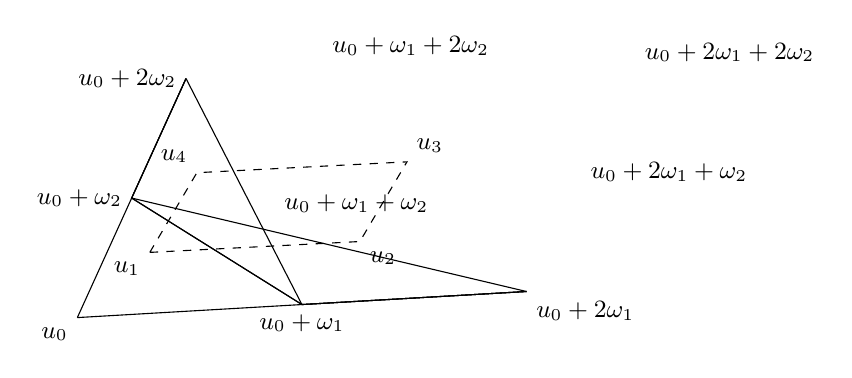
\begin{tikzpicture}[scale=0.92, every node/.style={font=\small}]
\coordinate (O) at (0,0);
\coordinate (A) at (3.1,0.18);
\coordinate (B) at (0.75,1.65);
\foreach \i in {0,1,2}{
  \draw (O)+(\i*3.1,\i*0.18) -- ++(0.75,1.65) -- ++(0.75,1.65);
}
\foreach \j in {0,1,2}{
  \draw (O)+(\j*0.75,\j*1.65) -- ++(3.1,0.18) -- ++(3.1,0.18);
}
\draw[dashed] (1.0,0.9) -- (3.9,1.05) -- (4.55,2.15) -- (1.65,2.0) -- cycle;
\node[below left] at (0,0) {$u_0$};
\node[below] at (3.1,0.18) {$u_0+\omega_1$};
\node[below right] at (6.2,0.36) {$u_0+2\omega_1$};
\node[left] at (0.75,1.65) {$u_0+\omega_2$};
\node[below] at (3.85,1.83) {$u_0+\omega_1+\omega_2$};
\node[right] at (6.95,2.01) {$u_0+2\omega_1+\omega_2$};
\node[left] at (1.5,3.3) {$u_0+2\omega_2$};
\node[above] at (4.6,3.48) {$u_0+\omega_1+2\omega_2$};
\node[right] at (7.7,3.66) {$u_0+2\omega_1+2\omega_2$};
\node[below left] at (1.0,0.9) {$u_1$};
\node[below right] at (3.9,1.05) {$u_2$};
\node[above right] at (4.55,2.15) {$u_3$};
\node[above left] at (1.65,2.0) {$u_4$};
\end{tikzpicture}
\caption{Fig. 1.}
\end{figure}


Thus Fig. 1 represents four period parallelograms laid alongside one another; the points $u_1,u_2,u_3,u_4$ are congruent:
\[
u_2=u_1+\omega_1,\qquad u_3=u_1+\omega_1+\omega_2,\qquad u_4=u_1+\omega_2,
\]
and $u_1,u_2,u_3,u_4$ likewise form the corners of a period parallelogram.

The doubly periodic function $\varphi(u)$ has the same value at all congruent points, and the entire stock of values of this function is therefore exhausted in one period parallelogram, if of two opposite sides only one is counted with the parallelogram.

From our general assumptions we draw the conclusion:

1. There exists, apart from the constant, no doubly periodic function which is free of points of discontinuity in the period parallelogram; for such a function would be finite in the whole $u$-plane and hence by \S\,15, 8 would have to be a constant.

If $\varphi(u)$ is a doubly periodic function with periods $\omega_1,\omega_2$, then the integral taken over the boundary of the period parallelogram is, because of (1),
\[
\int d\log\varphi(u)
=\int_{u_0}^{u_0+\omega_1}\!\!\left[d\log\varphi(u)-d\log\varphi(u+\omega_2)\right]
-\int_{u_0}^{u_0+\omega_2}\!\!\left[d\log\varphi(u)-d\log\varphi(u+\omega_1)\right]
=0.
\]
From this follows, by \S\,15, 6, the theorem:

2. A doubly periodic function becomes zero at just as many points in a period parallelogram as it becomes infinite. If $m$ is this number, then $m$ is called the order of the doubly periodic function. By 1. there are no doubly periodic functions of order zero.

If in the proof one replaces the function $\varphi(u)$ by $\varphi(u)-c$, it follows that a doubly periodic function of $m$th order assumes every arbitrary value $c$ at equally many points.

If we take the integral of the formula in 7., \S\,15 over the boundary of the period parallelogram, we obtain
\begin{align*}
\int u\,d\log\varphi(u)
&=\int_{u_0}^{u_0+\omega_1}\!\!\left[u\,d\log\varphi(u)-(u+\omega_2)d\log\varphi(u+\omega_2)\right]\\
&\quad-\int_{u_0}^{u_0+\omega_2}\!\!\left[u\,d\log\varphi(u)-(u+\omega_1)d\log\varphi(u+\omega_1)\right]\\
&=-\omega_2\int d\log\varphi(u)+\omega_1\int d\log\varphi(u).
\end{align*}
Now, because of the many-valuedness of the logarithm,
\[
\int d\log\varphi(u)=\log\varphi(u+\omega_1)-\log\varphi(u)=2\pi i m_1,
\]
\[
\int d\log\varphi(u)=\log\varphi(u+\omega_2)-\log\varphi(u)=-2\pi i m_2,
\]
where $m_1$ and $m_2$ are undetermined integers.

If therefore the function $\varphi(u)$ becomes infinite at the points $\alpha_1,\alpha_2,\ldots,\alpha_m$ and zero at the points $\beta_1,\beta_2,\ldots,\beta_m$, then, by \S\,15, 7,
\[
\sum \alpha \equiv \sum \beta\pmod{\omega_1,\omega_2}.
\]

If one replaces $\varphi(u)$ by $\varphi(u)-c$, where $c$ denotes an arbitrary value, the important theorem follows:

3. The sum of the argument values at which a doubly periodic function assumes one and the same value $c$ in the interior of a period parallelogram is independent of $c$, or changes under continuous variation of $c$ at most by jumps of a period.

4. From this it follows also that there is no doubly periodic function of the first order.

For such a function would have to assume every value $c$ at one point $u$. If it were therefore equal to $c'$ at a point $u'$ and equal to $c'$ at a different point $u''$, then by 3. $u'=u''$ would follow, contrary to the assumption.

By a doubly periodic function of the second kind one understands, following Hermite, a function $\psi(u)$ which, with respect to the periods $\omega_1,\omega_2$, behaves according to the equations
\[
\psi(u+\omega_1)=A_1\psi(u),\qquad
\psi(u+\omega_2)=A_2\psi(u),
\]
where $A_1,A_2$ are constants.

5. Also for a doubly periodic function of the second kind the theorem holds that it becomes zero and infinite at equally many points of the period parallelogram. If the number of these points is $m$, then here too the function is called of the $m$th order.

The proof is the same as that of theorem 2. But here the extension no longer holds that the function $\psi(u)$ assumes every value equally often, because $\psi(u)-c$ is no longer periodic.

6. A doubly periodic function $\psi(u)$ of the second kind and of order zero is necessarily a constant or an exponential function. For if $\psi(u)$ does not become zero, then
\[
\varphi(u)=\frac{\psi'(u)}{\psi(u)}
\]
is a doubly periodic function of the first kind which does not become infinite, and hence by 1. is a constant $a$. It follows that
\[
\psi(u)=Ae^{au},
\]
where $A$ is a new constant.

\section*{\S\,17. The functions $T$.}

If doubly periodic functions $\varphi(u)$ of the $m$th order exist, then they must be fractional functions. We therefore set them, according to \S\,15, 10, in the form
\begin{equation}
\varphi(u)=\frac{G_1(u)}{G(u)}.
\tag{1}
\end{equation}
If $G_1(u)$ and $G(u)$ are entire functions without a common zero, then
\[
\frac{G(u+\omega_1)}{G(u)}=\frac{G_1(u+\omega_1)}{G_1(u)},\qquad
\frac{G(u+\omega_2)}{G(u)}=\frac{G_1(u+\omega_2)}{G_1(u)}.
\]
In these equations the three functions $G(u)$, $G(u+\omega_1)$, $G(u+\omega_2)$ have the same $m$ zeros, namely the points of discontinuity of $\varphi(u)$. Their quotients are therefore unit functions, and by \S\,15, 9, if $l_1(u),l_2(u)$ are entire functions,
\begin{equation}
G(u+\omega_1)=e^{l_1(u)}G(u),\qquad
G(u+\omega_2)=e^{l_2(u)}G(u),
\tag{2}
\end{equation}
and the function $G_1(u)$ satisfies the same equations.

If
\begin{equation}
\varphi(u)=\frac{T_1(u)}{T(u)}
\tag{3}
\end{equation}
is a second representation of $\varphi(u)$ of the form (1), then
\begin{equation}
T(u)=e^{g(u)}G(u),
\tag{4}
\end{equation}
where $g(u)$ is again an entire function, and if therefore, by (2),
\begin{equation}
T(u+\omega_1)=e^{l'_1(u)}T(u),\qquad
T(u+\omega_2)=e^{l'_2(u)}T(u),
\tag{5}
\end{equation}
then
\[
l'_1(u)=l_1(u)+g(u)-g(u+\omega_1),\qquad
l'_2(u)=l_2(u)+g(u)-g(u+\omega_2).
\]

Everything therefore depends on being able, under some suitable assumption about the entire functions $l_1(u),l_2(u)$, to form entire functions $T(u)$ which satisfy the conditions (5) and vanish at $m$ arbitrarily given points of the period parallelogram. By the quotients of two such functions with the same $l_1(u),l_2(u)$ we can then represent all doubly periodic functions $\varphi(u)$, and the more general functions $G(u)$ which accomplish the same thing are obtained by (4) through adjoining an arbitrary unit factor.

If we wanted to assume $l_1(u),l_2(u)$ to be constants, then $T(u)$ would be an entire doubly periodic function of the second kind and consequently by \S\,16, 6 an exponential function, from which no doubly periodic functions can be formed. The simplest assumption that remains to us after this is that $l_1(u),l_2(u)$ are linear functions of $u$, including as a special case also the case that one of the two functions $l_1,l_2$ is constant.

Thus we set up the following definition:

1. A $T$-function, $T(u)$, is an entire function of $u$ which satisfies the following two equations:
\begin{equation}
\begin{aligned}
T(u+\omega_1)&=e^{-\pi i[a_1(2u+\omega_1)+b_1]}T(u),\\
T(u+\omega_2)&=e^{-\pi i[a_2(2u+\omega_2)+b_2]}T(u).
\end{aligned}
\tag{6}
\end{equation}
Here $a_1,b_1,a_2,b_2$ are constants, that is, magnitudes independent of $u$. The periods $\omega_1,\omega_2$ are taken here throughout as constants given once for all, whose ratio $\omega_2:\omega_1$ has a positive imaginary part.

The factors
\[
e_1=e_1(u)=e^{-\pi i[a_1(2u+\omega_1)+b_1]},\qquad
e_2=e_2(u)=e^{-\pi i[a_2(2u+\omega_2)+b_2]}
\]
are called the two periodicity factors of the function $T$.

The periodicity factors do not change if $b_1,b_2$ are changed by even integers. That functions of this kind really exist will first appear in the further course of the investigation.

2. If the function $T(u)$ vanishes at any point, then it also vanishes at all congruent points. If it vanishes at $m$ points of the period parallelogram, then it is called of the $m$th order.

From this definition it follows at once:

3. By multiplying two $T$-functions $T,T'$ of orders $m,m'$ one obtains a $T$-function of order $m+m'$. The periodicity factors of the product $TT'$ are the products of the periodicity factors of $T$ and $T'$.

We first ask about the possibility of $T$-functions of zeroth order. If $L(u)$ is such a function and $L'(u)$ its derivative, then by twice differentiating (6) it follows that
\[
\frac{dL(u+\omega_1)}{du\,L(u+\omega_1)}=\frac{dL(u)}{du\,L(u)},
\]
and correspondingly from the second equation (6). Hence $d^2\log L(u)/du^2$, as an entire doubly periodic function, is a constant, and consequently $\log L(u)$ is an entire function of the second degree in $u$. We therefore obtain:

4. A $T$-function of zeroth order is of the form
\begin{equation}
L(u)=Ce^{-\pi i(\lambda u^2+\mu u)},
\tag{7}
\end{equation}
where $\lambda,\mu,C$ are constants.

That every function of this form is a $T$-function of zeroth order is seen immediately.

The product
\begin{equation}
T'(u)=L(u)T(u)
\tag{8}
\end{equation}
is, like $T(u)$, a $T$-function of $m$th order and vanishes at the same points.

The periodicity factors of $T'$ are obtained from those of $T$ when the exponents $a_1,a_2,b_1,b_2$ are replaced by
\begin{equation}
a'_1=a_1+\lambda\omega_1,\quad
b'_1=b_1+\mu\omega_1,\qquad
a'_2=a_2+\lambda\omega_2,\quad
b'_2=b_2+\mu\omega_2,
\tag{9}
\end{equation}
where however the $b'_1,b'_2$ are determined only up to additive even integers.

5. By (9) one can determine $\mu$ always, and in only one way, so that $b'_1,b'_2$ become real.

For if one sets the imaginary parts of $b'_1,b'_2$ equal to zero, one obtains for the imaginary and real part of $\mu$ two linear equations whose determinant, by \S\,16, is the area of the period parallelogram and therefore different from zero.

The periodicity factors and the zeros of a $T$-function of $m$th order stand in a certain dependence on one another, which we obtain easily from the theorems of \S\,15. First the order $m$ is obtained when one extends the integral
\[
\int d\log T(u)=2\pi i\,m
\]
over the boundary of the period parallelogram. For simplicity let the corner $u_0$ lie at the origin of coordinates; then this integral can be decomposed as
\[
2\pi i m=\int_{0}^{\omega_1}d[\log T(u)-\log T(u+\omega_2)]
-\int_{0}^{\omega_2}d[\log T(u)-\log T(u+\omega_1)],
\]
and by (6)
\[
d[\log T(u)-\log T(u+\omega_2)]=2\pi i a_2,\qquad
d[\log T(u)-\log T(u+\omega_1)]=2\pi i a_1.
\]
It follows that
\begin{equation}
a_2\omega_1-a_1\omega_2=m.
\tag{10}
\end{equation}

If we further denote by $\alpha_1,\alpha_2,\ldots,\alpha_m$ the zeros of a $T$-function in the interior of a period parallelogram, then from \S\,15, 7 we obtain
\[
2\pi i\sum\alpha=\int u\,d\log T(u),
\]
when the integral is again extended over the boundary of the parallelogram. But
\begin{align*}
\int u\,d\log T(u)
&=\int_{0}^{\omega_1}\!\!\left[u\,d\log T(u)-(u+\omega_2)d\log T(u+\omega_2)\right]\\
&\quad-\int_{0}^{\omega_2}\!\!\left[u\,d\log T(u)-(u+\omega_1)d\log T(u+\omega_1)\right].
\end{align*}
The first of these two integrals is, by (6),
\begin{align*}
&-\omega_2\int_0^{\omega_1}d\log T(u)+2\pi i a_2\int_0^{\omega_1}(u+\omega_2)\,du\\
&\quad=-\omega_2[\log T(\omega_1)-\log T(0)]+\pi i a_2\omega_1(\omega_1+2\omega_2)\\
&\quad=\pi i\omega_2(a_1\omega_1+b_1)+\pi i a_2(\omega_1^2+2\omega_1\omega_2)+2\pi iN_2\omega_2,
\end{align*}
where $N_2$, because of the many-valuedness of the logarithm, is an integer not more closely determined. Likewise, for the second of the integrals one obtains
\[
-\pi i\omega_1(a_2\omega_2+b_2)-\pi i a_1(\omega_2^2+2\omega_1\omega_2)+2\pi iN_1\omega_1,
\]
and consequently, written as a congruence,
\begin{equation}
\sum\alpha\equiv \frac12(b_1\omega_2-b_2\omega_1)+\frac{m}{2}(\omega_1+\omega_2).
\tag{11}
\end{equation}

This sum, or rather the totality of the numbers congruent with it modulo $(\omega_1,\omega_2)$, is called the character of the $T$-function.

The character of the function $T$ is not changed if one replaces $T$ by one of the functions $LT$. Thus by 5. one can also represent the character in the form
\begin{equation}
\sum\alpha\equiv \frac12(g_1\omega_2-g_2\omega_1)+\frac{m}{2}(\omega_1+\omega_2),
\tag{12}
\end{equation}
where $g_1,g_2$ are real. These real numbers are determined by the character up to multiples of 2 and can take every value between 0 and 2. The symbol $(g_1,g_2)$ is called the characteristic of the $T$-function. From the characteristic the character of the $T$-function is determined by (12).

If $\gamma$ is the character of a function $T(u)$ of order $m$ and $v$ is an arbitrary constant, then $T(u+v)$ has the character
\[
\gamma'=\gamma-vm.
\]
Accordingly, when $m>0$, the different characters can be reduced to one another.

With the help of equation (10) one can combine the two equations (6) into a general one. If in the first equation (6) one repeatedly changes $u$ into $u+\omega_1$, one obtains the system
\[
T(u+\omega_1)=e^{-\pi i[a_1(2u+\omega_1)+b_1]}T(u),
\]
\[
T(u+2\omega_1)=e^{-\pi i[a_1(2u+3\omega_1)+b_1]}T(u+\omega_1),
\]
\[
T(u+n_1\omega_1)=e^{-\pi i[a_1(2u+(2n_1-1)\omega_1)+b_1]}T(u+(n_1-1)\omega_1),
\]
and by multiplication of all these formulae:
\begin{equation}
T(u+n_1\omega_1)=e^{-\pi i[a_1(2n_1u+n_1^2\omega_1)+n_1b_1]}T(u).
\tag{13}
\end{equation}
This formula is first derived for a positive integral $n_1$. But if in it one replaces $u$ by $u-n_1\omega_1$, its correctness for negative $n_1$ also results.

Likewise one obtains
\begin{equation}
T(u+n_2\omega_2)=e^{-\pi i[a_2(2n_2u+n_2^2\omega_2)+n_2b_2]}T(u),
\tag{14}
\end{equation}
and if in this formula one changes $u$ into $u+n_1\omega_1$ and again applies (13),
\begin{equation}
\begin{aligned}
T(u+n_1\omega_1+n_2\omega_2)
&=e^{-\pi i[2(a_1n_1+a_2n_2)u+2a_2n_1n_2\omega_1+a_1n_1^2\omega_1+a_2n_2^2\omega_2+n_1b_1+n_2b_2]}T(u).
\end{aligned}
\tag{15}
\end{equation}
But by (10)
\[
2a_2n_1n_2\omega_1=a_1n_1n_2\omega_1+a_2n_1n_2\omega_2+mn_1n_2,
\]
and therefore this last formula becomes
\begin{equation}
T(u+n_1\omega_1+n_2\omega_2)
=e^{-\pi i[(n_1a_1+n_2a_2)(2u+n_1\omega_1+n_2\omega_2)+b_1n_1+b_2n_2+mn_1n_2]}T(u).
\tag{16}
\end{equation}
Here $n_1$ and $n_2$ are arbitrary positive or negative integers.

If one multiplies two $T$-functions of order $m$ and $m'$ and of characters $\gamma,\gamma'$, there arises a new $T$-function whose order is $m+m'$ and whose character is $\gamma+\gamma'$. If $(g_1,g_2)$ and $(g'_1,g'_2)$ are the characteristics of the two factors, then $(g_1+g'_1,g_2+g'_2)$ is the characteristic of the product.

\section*{\S\,18. Relations between related $T$-functions.}

Two $T$-functions with the same periods, the same order, and the same character shall be called related. If $T'(u)$ is a $T$-function related to $T(u)$, and if $a'_1,a'_2,b'_1,b'_2$ have the same meaning for $T'$ as $a_1,a_2,b_1,b_2$ for $T$, then, in consequence of the assumed relatedness,
\begin{align}
a'_1\omega_2-a'_2\omega_1&=a_1\omega_2-a_2\omega_1,\tag{1}\\
b'_1\omega_2-b'_2\omega_1&=b_1\omega_2-b_2\omega_1+2n_1\omega_2-2n_2\omega_1,\tag{2}
\end{align}
where $n_1,n_2$ are integers.

Therefore $\lambda$ and $\mu$ can be determined according to \S\,17, (9) so that the periodicity factors of the function
\[
e^{-\pi i(\lambda u^2+\mu u)}T(u)
\]
become the same as those of the function $T'(u)$, and hence we have the theorem:

1. Related $T$-functions can, by adjoining a $T$-function of zeroth order
\[
L=Ce^{-\pi i(\lambda u^2+\mu u)}
\]
as factor, be given the same periodicity factors.

Furthermore, from the equality of the characters it follows immediately:

2. If related $T$-functions of $m$th order have $m-1$ common zeros in the period parallelogram, then they also have the $m$th in common; and from this:

3. Between at most $m+1$ related $T$-functions of $m$th order $T,T_1,\ldots,T_m$ there exists an identical equation of the form
\[
LT+L_1T_1+L_2T_2+\cdots+L_mT_m=0.
\]
For if this relation does not already hold for $L=0$, then one can first determine the constants available in $L_1,L_2,\ldots,L_m$ so that all the products $L_1T_1,L_2T_2,\ldots,L_mT_m$ receive the same periodicity factors, and then the remaining constants so that $m-1$, and consequently all, zeros of the function $L_1T_1+L_2T_2+\cdots+L_mT_m$ coincide with the zeros of the function $T$. From this, however, it follows that the ratio of $L_1T_1+L_2T_2+\cdots+L_mT_m$ to $T$ is equal to a $T$-function of zeroth order, thus equal to $-L$, as was to be proved.

4. The quotients of related $T$-functions can be transformed into doubly periodic functions by adjoining a factor $L$.

5. If we assume the existence of a $T$-function of the first order $t(u)$, then every $T$-function of $m$th order can be derived from it.

Namely, let $\gamma$ be the character of $t(u)$ and let $\alpha_1,\alpha_2,\ldots,\alpha_m$ be arbitrarily given values. Then the function
\[
t(u-\alpha_i+\gamma)=t_i(u)
\]
vanishes at the point $\alpha_i$ and all points congruent with $\alpha_i$, but at no other.

The product
\[
T(u)=t_1(u)t_2(u)\cdots t_m(u)
\]
is therefore a $T$-function of $m$th order with the arbitrarily given zeros $\alpha_1,\alpha_2,\ldots,\alpha_m$.

6. From this it is easy to prove that every doubly periodic function which has only a finite number of points of discontinuity in a period parallelogram can be represented as the quotient of two $T$-functions.

Let $\varphi(u)$ be a doubly periodic function with periods $\omega_1,\omega_2$ and with points of discontinuity $\alpha_1,\alpha_2,\ldots,\alpha_m$, which may also partly coincide to points of discontinuity of higher order.

If according to 5. one determines a function $T(u)$ with zeros $\alpha_1,\alpha_2,\ldots,\alpha_m$, then
\[
T(u)\varphi(u)=T_1(u)
\]
is a $T$-function of $m$th order, and
\[
\varphi(u)=\frac{T_1(u)}{T(u)}.
\]
The functions $T(u),T_1(u)$ are related, since they have the same periodicity factors and hence also the same characteristic.

The zeros of $T_1(u)$ are at the same time the zeros of $\varphi(u)$, and the sum of these zero values is therefore congruent with the sum of the discontinuity values.

\section*{\S\,19. $T$-functions of first order.}

We now pass to the closer determination of the $T$-functions of first order, which we denote by $t(u)$, and from which, as we have seen, the remaining $T$-functions can be derived.

From 3. of the preceding paragraph it follows that two $t$-functions of the same characteristic differ only by a factor of the form
\[
Ce^{-\pi i(\lambda u^2+\mu u)},
\]
and we shall now, by an extension of the definition, determine this factor still more closely.

This shall be done, as is possible without restriction of generality by \S\,17, (9), so that in the periodicity factors
\[
a_1=0,\qquad b_1=g_1,\qquad b_2=g_2
\]
when $(g_1,g_2)$ is the characteristic; because of the relation
\[
a_2\omega_1-a_1\omega_2=1
\]
one then has
\[
a_2=\frac{1}{\omega_1},
\]
and the conditions for this $t$-function read:
\begin{equation}
t(u+\omega_1)=e^{-\pi i g_1}t(u),\qquad
t(u+\omega_2)=e^{-\pi i\frac{2u+\omega_2}{\omega_1}}e^{-\pi i g_2}t(u).
\tag{1}
\end{equation}
By this the function $t(u)$ is determined up to a factor independent of $u$. In order to determine this factor still more closely, we consider also the dependence of the function $t$ on $\omega_1,\omega_2$, and denote it, regarding $g_1,g_2$ as given numbers independent of $\omega_1,\omega_2$, by $t(u,\omega_1,\omega_2)$. It then appears that if $h$ is an arbitrary factor,
\[
t(hu,h\omega_1,h\omega_2)
\]
likewise satisfies the conditions (1), and hence that
\begin{equation}
\frac{t(hu,h\omega_1,h\omega_2)}{t(u,\omega_1,\omega_2)}=f(\omega_1,\omega_2)
\tag{2}
\end{equation}
is independent of $u$.

But the function $f(\omega_1,\omega_2)$ can always be put into the form
\[
f(\omega_1,\omega_2)=\frac{\varphi(h\omega_1,h\omega_2)}{\varphi(\omega_1,\omega_2)}.
\]
One has only, if $t(u)$ does not vanish for $u=0$, to put
\[
\varphi(\omega_1,\omega_2)=t(0,\omega_1,\omega_2),
\]
and if $t(0)=0$, for instance
\[
\varphi(\omega_1,\omega_2)=\omega_1t'(0,\omega_1,\omega_2),
\]
where $t'$ denotes the derivative of $t$ with respect to $u$. If therefore we now again denote
\begin{equation}
\frac{t(u,\omega_1,\omega_2)}{\varphi(\omega_1,\omega_2)}
\tag{3}
\end{equation}
by $t(u,\omega_1,\omega_2)$, then one can add to the conditions (1) the condition that for an arbitrary $h$
\begin{equation}
t(u,\omega_1,\omega_2)=t(hu,h\omega_1,h\omega_2).
\tag{4}
\end{equation}

The function $t$ now depends only on two variables, namely the ratios $u:\omega_1:\omega_2$. We put in (4)
\[
h=\frac1{\omega_1},\qquad \frac{u}{\omega_1}=v,\qquad \frac{\omega_2}{\omega_1}=\omega,
\]
and obtain
\begin{equation}
t(u,\omega_1,\omega_2)=\vartheta\!\left(\frac{u}{\omega_1},\frac{\omega_2}{\omega_1}\right)=\vartheta(v,\omega),
\tag{5}
\end{equation}
where $\vartheta$ is a new function sign.

Thus a new function $\vartheta(v)$ is defined, of only two variables $v,\omega$, the first of which is unrestrictedly variable, while $\omega$ has, by the assumption made in \S\,16, a positive imaginary constituent; $v$ is called the argument, $\omega$ the modulus of the $\vartheta$-function.

\section*{\S\,20. The $\vartheta$-function.}

The function $\vartheta(v)$ is an entire function of $v$ which satisfies the conditions
\begin{equation}
\vartheta(v+1)=e^{-\pi i g_1}\vartheta(v),\qquad
\vartheta(v+\omega)=e^{-\pi i(2v+\omega)}e^{-\pi i g_2}\vartheta(v),
\tag{1}
\end{equation}
and is thereby determined up to a factor independent of $v$. It is therefore included among the $t$-functions as a special case, while conversely the general $t$-function can be expressed by the $\vartheta$-function in the way
\[
t(u)=Ce^{-\pi i(\lambda u^2+\mu u)}
\vartheta\!\left(\frac{u}{\omega_1},\frac{\omega_2}{\omega_1}\right),
\]
where $C,\lambda,\mu$ are arbitrary magnitudes, constant or depending on $\omega_1,\omega_2$.

The function $\vartheta$ still depends on the numbers $g_1,g_2$ occurring in the characteristic, and if a notation for this dependence is necessary, one shall write for $\vartheta(v,\omega)$
\[
\vartheta_{g_1,g_2}(v,\omega);
\]
here $g_1,g_2$ may be arbitrary numbers. By what was said earlier it is enough if we assume them real and between 0 and 2.

Corresponding to the $T$-functions of higher order we shall also introduce $\Theta$-functions of $m$th order, and understand by this an entire function of $v$ which satisfies the conditions
\begin{equation}
\Theta(v+1)=e^{-\pi i g_1}\Theta(v),\qquad
\Theta(v+\omega)=e^{-m\pi i(2v+\omega)}e^{-\pi i g_2}\Theta(v).
\tag{2}
\end{equation}
Here also the characteristic $g_1,g_2$ can be included in the notation:
\[
\Theta_{g_1,g_2}(v,\omega).
\]

These functions are contained as special cases among the $T$-functions, and one can form general $T$-functions in the way
\begin{equation}
Ce^{-\pi i(\lambda u^2+\mu u)}
\Theta\!\left(\frac{u}{\omega_1},\frac{\omega_2}{\omega_1}\right).
\tag{3}
\end{equation}

Thus from \S\,18, 3 there results the fundamental theorem for the $\Theta$-functions, which we state as follows.

If we call $\Theta$-functions with the same periods, equal order, and equal characteristic related, and if furthermore we call a system of functions linearly dependent or independent according as a homogeneous linear relation with constant coefficients, not all vanishing, exists between these functions or not, then the theorem holds:

\[
m+1 \text{ related } \Theta\text{-functions of } m\text{th order are always linearly dependent;}
\]
or:
\[
\text{from } m \text{ linearly independent related } \Theta\text{-functions of } m\text{th order}
\]
every other related $\Theta$-function can be linearly composed, with constant coefficients.

This theorem is of the most fundamental importance for our following considerations; from it, by \S\,18, 3, it follows that every $T$-function of $m$th order can, by use of formula (3), be composed out of $m$ linearly independent $\Theta$-functions.

By \S\,17, (11), the sum of the $m$ argument values for which the function $\Theta_{g_1,g_2}(v)$ vanishes in the period parallelogram is congruent modulo $(1,\omega)$ to
\[
m\frac{1+\omega}{2}+\frac{g_1\omega-g_2}{2}.
\]

The definition of the function $\vartheta$ given up to now leaves undetermined a factor which may be a function of $\omega$. But by an addition to the definition we can determine this factor more closely.

If the defining equations (1) are differentiated twice with respect to $v$ and once with respect to $\omega$, regarding $g_1,g_2$ as constants, then by a simple calculation it follows that the function
\[
\frac{\partial^2\vartheta(v,\omega)}{\partial v^2}-4\pi i\,\frac{\partial\vartheta(v,\omega)}{\partial\omega}
\]
itself satisfies the conditions (1), and therefore has the form
\[
\varphi(\omega)\vartheta(v,\omega),
\]
where $\varphi(\omega)$ is constant with respect to $v$, hence a function of $\omega$ alone. If one now sets
\[
e^{-\frac{1}{4\pi i}\int \varphi(\omega)\dd\omega}\vartheta(v,\omega)
\]
equal to a new $\vartheta$, then for this one obtains the partial differential equation
\begin{equation}
\frac{\partial^2\vartheta(v,\omega)}{\partial v^2}-4\pi i\,\frac{\partial\vartheta(v,\omega)}{\partial\omega}=0,
\tag{4}
\end{equation}
and by (1) and (4) the function $\vartheta$ is now defined up to a factor independent of $v$ and $\omega$, thus depending only on $g_1,g_2$.

\section*{\S\,21. The theta functions of different characteristics. Main characteristics.}

Before we go on to the determination of the remaining factor in the $\vartheta$-functions that is independent of $v$ and $\omega$, we shall now reduce the different characteristics to one another, which by \S\,17 is always possible. If $\vartheta(v)$ denotes the $\vartheta$-function belonging to the characteristic $(0,0)$, then
\[
\Phi(v,\omega)=e^{-\pi i g_1 v}\,
\vartheta\!\left(v-\frac{g_1\omega-g_2}{2}\right)
\]
is a function satisfying the conditions (1) of \S\,20. But, with regard to the differential equation (4), one has
\[
\frac{\partial^2\Phi}{\partial v^2}-4\pi i\,\frac{\partial\Phi}{\partial\omega}
=-\pi^2g_1^2\Phi,
\]
and if therefore we put
\begin{equation}
\vartheta_{g_1,g_2}(v)
=e^{\frac{\pi i\omega g_1^2}{4}-\pi i g_1v+\frac{g_1g_2\pi i}{2}}\,
\vartheta\!\left(v-\frac{g_1\omega-g_2}{2}\right),
\tag{1}
\end{equation}
then the differential equation (4) of \S\,20 is satisfied by all these functions. Thus the functions $\vartheta_{g_1,g_2}$ are determined up to one numerical factor common to all.

From formula (1) a more general formula can be derived by replacing $v$ by
\[
v-\frac{g'_1\omega-g'_2}{2}.
\]
One obtains
\begin{equation}
\vartheta_{g_1,g_2}\!\left(v-\frac{g'_1\omega-g'_2}{2}\right)
=e^{-\frac{\pi i\omega}{4}g_1'^2+\pi i g'_1v-\pi i g_1g'_2-\frac{\pi i}{2}g'_1(g_2+g'_2)}
\vartheta_{g_1+g'_1,g_2+g'_2}(v).
\tag{2}
\end{equation}

From (2) there also follows, using (1) of \S\,20, if one sets $g'_1=2,g'_2=0$, or $g'_1=0,g'_2=2$:
\begin{equation}
\vartheta_{g_1+2,g_2}(v)=e^{2\pi i g_2}\vartheta_{g_1,g_2}(v),\qquad
\vartheta_{g_1,g_2+2}(v)=e^{\pi i g_1}\vartheta_{g_1,g_2}(v),
\tag{3}
\end{equation}
and by (2) at the same time the periodicity of the functions $\vartheta_{g_1,g_2}(v)$ is completely expressed. For example, if $\mu$ and $\nu$ are integers, one obtains
\begin{equation}
\vartheta_{00}\!\left(v-\frac{(2\nu-1)\omega+2\mu-1}{2}\right)
=(-1)^{\nu+1}i\,e^{-\frac{\pi i\omega}{4}(2\nu-1)^2}e^{\pi i(2\nu-1)v}\vartheta_{11}(v),
\tag{4}
\end{equation}
\begin{equation}
\vartheta_{11}(v-\nu\omega-\mu)=(-1)^{\mu+\nu}e^{-\pi i\omega\nu^2}e^{2\pi i\nu v}\vartheta_{11}(v).
\tag{5}
\end{equation}
Formula (2) is valid for quite arbitrary, even complex, values of $g_1,g_2$.

If in the defining formulae of the $\vartheta$-functions \S\,20, (1) one replaces $v$ by $-v-1$ and by $-v-\omega$, and also replaces $g_1,g_2$ by $-g_1,-g_2$, then it is seen that $\vartheta_{-g_1,-g_2}(-v)$ satisfies the same conditions as $\vartheta_{g_1,g_2}(v)$, and hence that
\[
\vartheta_{g_1,g_2}(v),\qquad \vartheta_{-g_1,-g_2}(-v)
\]
are identical up to a constant factor; in particular, as follows from $v=0$,
\[
\vartheta_{0,0}(v)=\vartheta_{0,0}(-v),
\]
and then formula (1), when $v,g_1,g_2$ are replaced by $-v,-g_1,-g_2$, gives
\begin{equation}
\vartheta_{g_1,g_2}(v)=\vartheta_{-g_1,-g_2}(-v).
\tag{6}
\end{equation}

If the elements $g_1,g_2$ are integers, then $(g_1,g_2)$ is called a main characteristic. There are four essentially different ones, namely
\[
(0,0),\qquad (0,1),\qquad (1,0),\qquad (1,1),
\]
and therefore also four essentially different main $\vartheta$-functions:
\begin{equation}
\vartheta_{00}(v),\qquad \vartheta_{01}(v),\qquad \vartheta_{10}(v),\qquad \vartheta_{11}(v),
\tag{7}
\end{equation}
of which the first is also denoted by $\vartheta(v)$.

In what follows, by characteristics and $\vartheta$-functions only main characteristics and main functions will be meant.

Formula (2), applied to this system of functions, gives the following frequently used table:
\begin{align}
\vartheta_{00}(v)&=\vartheta_{01}\!\left(v+\frac12\right)=\eps\,\vartheta_{10}\!\left(v+\frac{\omega}{2}\right)=\eps\,\vartheta_{11}\!\left(v+\frac{1+\omega}{2}\right),\notag\\
\vartheta_{01}(v)&=\vartheta_{00}\!\left(v+\frac12\right)=-i\eps\,\vartheta_{11}\!\left(v+\frac{\omega}{2}\right)=i\eps\,\vartheta_{10}\!\left(v+\frac{1+\omega}{2}\right),\notag\\
\vartheta_{10}(v)&=\vartheta_{11}\!\left(v+\frac12\right)=\eps\,\vartheta_{00}\!\left(v+\frac{\omega}{2}\right)=\eps\,\vartheta_{01}\!\left(v+\frac{1+\omega}{2}\right),\tag{8}\\
\vartheta_{11}(v)&=-\vartheta_{10}\!\left(v+\frac12\right)=-i\eps\,\vartheta_{01}\!\left(v+\frac{\omega}{2}\right)=-i\eps\,\vartheta_{00}\!\left(v+\frac{1+\omega}{2}\right),
\notag
\end{align}
where, as an abbreviation,
\[
\eps=e^{\frac{\pi i\omega}{4}+\pi i v}
\]
is put.

By (3), (4),
\begin{equation}
\vartheta_{00}(-v)=\vartheta_{00}(v),\quad
\vartheta_{01}(-v)=\vartheta_{01}(v),\quad
\vartheta_{10}(-v)=\vartheta_{10}(v),\quad
\vartheta_{11}(-v)=-\vartheta_{11}(v),
\tag{9}
\end{equation}
that is, $\vartheta_{00}(v),\vartheta_{01}(v),\vartheta_{10}(v)$ are even functions, while $\vartheta_{11}(v)$ is an odd function.

By \S\,17, (12), the four functions (7) vanish respectively for the following values of the argument
\[
\frac{1+\omega}{2},\qquad \frac{\omega}{2},\qquad \frac12,\qquad 0,
\]
thus for certain half-periods. Of importance are the values which all the functions (7) assume for these argument values, and these can be reduced by means of table (8) to the three
\[
\vartheta_{00}(0)=\vartheta_{00},\qquad
\vartheta_{01}(0)=\vartheta_{01},\qquad
\vartheta_{10}(0)=\vartheta_{10}.
\]
Thus from (8) one obtains the following system of formulae:
\begin{align}
\vartheta_{00}&=\vartheta_{01}\!\left(\frac12\right)=\eps_0\vartheta_{10}\!\left(\frac{\omega}{2}\right)=\eps_0\vartheta_{11}\!\left(\frac{1+\omega}{2}\right),\notag\\
\vartheta_{01}&=\vartheta_{00}\!\left(\frac12\right)=-i\eps_0\vartheta_{11}\!\left(\frac{\omega}{2}\right)=i\eps_0\vartheta_{10}\!\left(\frac{1+\omega}{2}\right),\tag{10}\\
\vartheta_{10}&=\vartheta_{11}\!\left(\frac12\right)=\eps_0\vartheta_{00}\!\left(\frac{\omega}{2}\right)=\eps_0\vartheta_{01}\!\left(\frac{1+\omega}{2}\right),
\notag
\end{align}
where
\[
\eps_0=e^{\frac{\pi i\omega}{4}},
\]
and
\begin{equation}
\vartheta_{11}(0)=0,\quad
\vartheta_{10}\!\left(\frac12\right)=0,\quad
\vartheta_{01}\!\left(\frac{\omega}{2}\right)=0,\quad
\vartheta_{00}\!\left(\frac{1+\omega}{2}\right)=0.
\tag{11}
\end{equation}

The squares of the functions (7),
\begin{equation}
\vartheta_{00}^2(v),\quad \vartheta_{01}^2(v),\quad
\vartheta_{10}^2(v),\quad \vartheta_{11}^2(v),
\tag{12}
\end{equation}
are $\Theta_{00}$-functions of the second order, and consequently there are two linear relations between them. If we assume these relations in the form
\[
\vartheta_{10}^2(v)=A\vartheta_{01}^2(v)+B\vartheta_{11}^2(v),\qquad
\vartheta_{00}^2(v)=A'\vartheta_{01}^2(v)+B'\vartheta_{11}^2(v),
\]
then the coefficients can be easily determined on the basis of formulae (10), (11), if one sets $v=0$ and $v=\frac{\omega}{2}$. Thus one obtains
\begin{equation}
\vartheta_{01}^2\vartheta_{10}^2(v)=\vartheta_{10}^2\vartheta_{01}^2(v)-\vartheta_{00}^2\vartheta_{11}^2(v),\qquad
\vartheta_{01}^2\vartheta_{00}^2(v)=\vartheta_{00}^2\vartheta_{01}^2(v)-\vartheta_{10}^2\vartheta_{11}^2(v),
\tag{13}
\end{equation}
and from this also, putting $v=\frac12$,
\begin{equation}
\vartheta_{00}^4=\vartheta_{01}^4+\vartheta_{10}^4.
\tag{14}
\end{equation}

By any two of the squares (12) all functions $\Theta_{00}$ of the second order can be represented linearly; but the remaining $\Theta$-functions of the second order can also be composed from the functions $\vartheta_{g_1,g_2}$, for for each characteristic one obtains two linearly independent products, of which one is an even and the other an odd function, namely:
\begin{equation}
\begin{array}{rcll}
\vartheta_{00}(v)\vartheta_{01}(v),& \vartheta_{10}(v)\vartheta_{11}(v) &\quad& \text{characteristic }(0,1),\\
\vartheta_{00}(v)\vartheta_{10}(v),& \vartheta_{01}(v)\vartheta_{11}(v) && (1,0),\\
\vartheta_{10}(v)\vartheta_{01}(v),& \vartheta_{00}(v)\vartheta_{11}(v) && (1,1).
\end{array}
\tag{15}
\end{equation}

By the same principle all $\Theta$-functions of arbitrary order and arbitrary main characteristic can now be formed from the functions $\vartheta$. To prove this, we denote by $\Theta_0,\Theta_1$ any two of the $\vartheta$-squares (12), and by $F^{(n)}(\Theta_0,\Theta_1)$ an entire rational homogeneous function of $n$th order of the two arguments $\Theta_0,\Theta_1$. We obtain hereafter for the $\Theta$-functions of $m$th order $\Theta^{(m)}(v)$ the following expressions.

For even $m$:
\begin{equation}
\begin{array}{ll}
\text{even functions:}&\\[0.3em]
\Theta^{(m)}_{00}(v)=F^{(m/2)}(\Theta_0,\Theta_1),&
\Theta^{(m)}_{01}(v)=\vartheta_{00}(v)\vartheta_{01}(v)F^{(m/2-1)}(\Theta_0,\Theta_1),\\[0.3em]
\Theta^{(m)}_{10}(v)=\vartheta_{00}(v)\vartheta_{10}(v)F^{(m/2-1)}(\Theta_0,\Theta_1),&
\Theta^{(m)}_{11}(v)=\vartheta_{10}(v)\vartheta_{01}(v)F^{(m/2-1)}(\Theta_0,\Theta_1),\\[0.8em]
\text{odd functions:}&\\[0.3em]
\Theta^{(m)}_{00}(v)=\vartheta_{00}(v)\vartheta_{10}(v)\vartheta_{01}(v)\vartheta_{11}(v)F^{((m-4)/2)}(\Theta_0,\Theta_1),&\\[0.3em]
\Theta^{(m)}_{01}(v)=\vartheta_{10}(v)\vartheta_{11}(v)F^{(m/2-1)}(\Theta_0,\Theta_1),&
\Theta^{(m)}_{10}(v)=\vartheta_{01}(v)\vartheta_{11}(v)F^{(m/2-1)}(\Theta_0,\Theta_1),\\[0.3em]
\Theta^{(m)}_{11}(v)=\vartheta_{00}(v)\vartheta_{11}(v)F^{(m/2-1)}(\Theta_0,\Theta_1).&
\end{array}
\tag{16}
\end{equation}

For odd $m$:
\begin{equation}
\begin{array}{ll}
\text{even functions:}&\\[0.3em]
\Theta^{(m)}_{00}(v)=\vartheta_{00}(v)F^{((m-1)/2)}(\Theta_0,\Theta_1),&
\Theta^{(m)}_{01}(v)=\vartheta_{01}(v)F^{((m-1)/2)}(\Theta_0,\Theta_1),\\[0.3em]
\Theta^{(m)}_{10}(v)=\vartheta_{10}(v)F^{((m-1)/2)}(\Theta_0,\Theta_1),&
\Theta^{(m)}_{11}(v)=\vartheta_{00}(v)\vartheta_{01}(v)\vartheta_{10}(v)F^{((m-3)/2)}(\Theta_0,\Theta_1),\\[0.8em]
\text{odd functions:}&\\[0.3em]
\Theta^{(m)}_{00}(v)=\vartheta_{01}(v)\vartheta_{10}(v)\vartheta_{11}(v)F^{((m-3)/2)}(\Theta_0,\Theta_1),&\\[0.3em]
\Theta^{(m)}_{01}(v)=\vartheta_{00}(v)\vartheta_{10}(v)\vartheta_{11}(v)F^{((m-3)/2)}(\Theta_0,\Theta_1),&\\[0.3em]
\Theta^{(m)}_{10}(v)=\vartheta_{00}(v)\vartheta_{01}(v)\vartheta_{11}(v)F^{((m-3)/2)}(\Theta_0,\Theta_1),&
\Theta^{(m)}_{11}(v)=\vartheta_{11}(v)F^{((m-1)/2)}(\Theta_0,\Theta_1).
\end{array}
\tag{17}
\end{equation}

That all $\Theta$-functions are representable in this form follows, on the basis of \S\,20, from the following three considerations.

1. Between even and odd functions no linear dependence can exist unless a linear dependence already exists between the even functions alone or between the odd functions alone.

2. Since two of the $\vartheta$-squares (12) do not stand in a constant ratio, there also exists no equation of the form
\[
F^{(n)}(\Theta_0,\Theta_1)=0.
\]

3. The total number of constants which occur, according to (16), (17), in the even and odd functions belonging to one and the same characteristic is exactly equal to the order $m$.


\section*{\S\,22. The addition theorem.}

If $u,v$ are two variables, then the products
\[
\tht_{g_1,g_2}(u+v)\tht_{g'_1,g'_2}(u-v)
\]
belong to the $\Theta$-functions of the second order, with characteristic
\[
(g_1+g'_1,\,g_2+g'_2),
\]
and indeed for each of the two variables $u,v$; regarded as functions of $v$ they are therefore linearly representable by the functions (12) and (15) of \S\,21, so that the variable $u$ occurs in the coefficients. When the characteristic is $(0,0)$ this representation is possible in several ways, since one can choose two arbitrary functions from (12); in the other cases it is possible in only one way. One obtains in this manner sixteen formulae, of which, however, six can be derived from the others by mere interchange of $v$ with $-v$, so that only ten essentially different formulae remain. These formulae are very easily derived by first writing them with undetermined coefficients and then determining these coefficients by putting for $v$ such special values for which one of the functions $\tht(v)$ vanishes. Thus, for example,
\[
\tht_{00}(u+v)\tht_{00}(u-v)=A\tht_{00}^{2}(v)+B\tht_{11}^{2}(v),
\]
and if one puts $v=0$ and $v=(1+\omega)/2$, one obtains, using the formulae of \S\,21,
\[
A\tht_{00}^{2}=\tht_{00}^{2}(u),\qquad B\tht_{00}^{2}=\tht_{11}^{2}(u),
\]
and hence
\begin{equation}
\tht_{00}^{2}\tht_{00}(u+v)\tht_{00}(u-v)
=\tht_{00}^{2}(u)\tht_{00}^{2}(v)+\tht_{11}^{2}(u)\tht_{11}^{2}(v).
\tag{1}
\end{equation}
If one replaces $u$ in this by
\[
u+\frac12,\qquad u+\frac{\omega}{2},\qquad u+\frac{1+\omega}{2},
\]
one obtains three further relations, which could also have been derived directly in the same way as (1):
\begin{align}
\tht_{11}^{2}\tht_{01}(u+v)\tht_{01}(u-v)
&=\tht_{01}^{2}(u)\tht_{01}^{2}(v)-\tht_{11}^{2}(u)\tht_{11}^{2}(v), \tag{2}\\
\tht_{11}^{2}\tht_{10}(u+v)\tht_{10}(u-v)
&=\tht_{10}^{2}(u)\tht_{10}^{2}(v)-\tht_{11}^{2}(u)\tht_{11}^{2}(v), \tag{3}\\
\tht_{01}^{2}\tht_{11}(u+v)\tht_{11}(u-v)
&=\tht_{11}^{2}(u)\tht_{01}^{2}(v)-\tht_{01}^{2}(u)\tht_{11}^{2}(v). \tag{4}
\end{align}

These four equations can, as already mentioned, be transformed in many ways by applying the formulae (13) of the preceding paragraph. The following six formulae have only one form. It is, to begin again with an arbitrary example,
\[
\tht_{00}(u+v)\tht_{11}(u-v)=A\tht_{01}(v)\tht_{10}(v)+B\tht_{00}(v)\tht_{11}(v),
\]
and if one puts $v=0$,
\[
A\tht_{01}\tht_{10}=\tht_{00}(u)\tht_{11}(u);
\]
from this one obtains $B$ by interchanging $u$ with $v$. Thus the three following formulae are derived:
\begin{align}
\tht_{01}\tht_{10}\tht_{00}(u+v)\tht_{11}(u-v)
&=\tht_{00}(u)\tht_{11}(u)\tht_{01}(v)\tht_{10}(v)
 -\tht_{01}(u)\tht_{10}(u)\tht_{00}(v)\tht_{11}(v), \tag{5}\\
\tht_{00}\tht_{01}\tht_{10}(u+v)\tht_{11}(u-v)
&=\tht_{10}(u)\tht_{11}(u)\tht_{00}(v)\tht_{01}(v)
 -\tht_{00}(u)\tht_{01}(u)\tht_{10}(v)\tht_{11}(v), \tag{6}\\
\tht_{00}\tht_{10}\tht_{01}(u+v)\tht_{11}(u-v)
&=\tht_{01}(u)\tht_{11}(u)\tht_{00}(v)\tht_{10}(v)
 -\tht_{00}(u)\tht_{10}(u)\tht_{01}(v)\tht_{11}(v), \tag{7}
\end{align}
which are verified immediately by putting first $u$, then $v$, equal to zero. From these the three others follow by increasing $u$ by
\[
\frac12,\qquad \frac{\omega}{2},\qquad \frac12:
\]
\begin{align}
\tht_{01}\tht_{10}\tht_{01}(u+v)\tht_{10}(u-v)
&=\tht_{01}(u)\tht_{10}(u)\tht_{01}(v)\tht_{10}(v)
 +\tht_{00}(u)\tht_{11}(u)\tht_{00}(v)\tht_{11}(v), \tag{8}\\
\tht_{00}\tht_{01}\tht_{00}(u+v)\tht_{01}(u-v)
&=\tht_{00}(u)\tht_{01}(u)\tht_{00}(v)\tht_{01}(v)
 -\tht_{10}(u)\tht_{11}(u)\tht_{10}(v)\tht_{11}(v), \tag{9}\\
\tht_{00}\tht_{10}\tht_{00}(u+v)\tht_{10}(u-v)
&=\tht_{00}(u)\tht_{10}(u)\tht_{00}(v)\tht_{10}(v)
 +\tht_{01}(u)\tht_{11}(u)\tht_{01}(v)\tht_{11}(v). \tag{10}
\end{align}

The formulae whose totality is designated by the name of the addition theorem can be generalized in many ways; the following may serve as an example.

If $u,v$ are two variables, then the four products
\[
\tht_{00}(u)\tht_{00}(u+v),\quad
\tht_{01}(u)\tht_{01}(u+v),\quad
\tht_{10}(u)\tht_{10}(u+v),\quad
\tht_{11}(u)\tht_{11}(u+v),
\]
regarded as functions of $u$, are related $T$-functions of the second order with the same periodicity factors, and hence any three of them are linearly dependent. Thus
\[
A\tht_{00}(u)\tht_{00}(u+v)+B\tht_{10}(u)\tht_{10}(u+v)+C\tht_{11}(u)\tht_{11}(u+v)=0,
\]
from which, for $u=0$, $u=\frac12$,
\[
A\tht_{00}\tht_{00}(v)+B\tht_{10}\tht_{10}(v)=0,
\qquad
A\tht_{01}\tht_{01}(v)+C\tht_{10}\tht_{10}(v)=0,
\]
and hence
\begin{equation}
\tht_{10}\tht_{10}(v)\tht_{00}(u)\tht_{00}(u+v)
-\tht_{00}\tht_{00}(v)\tht_{10}(u)\tht_{10}(u+v)
-\tht_{01}\tht_{01}(v)\tht_{11}(u)\tht_{11}(u+v)=0.
\tag{11}
\end{equation}

Likewise, if $w$ is a third variable, the products contained in the form
\[
\tht_{g_1,g_2}(u+v)\tht_{g_1,g_2}(u+w),\qquad
\tht_{g_1,g_2}(u)\tht_{g_1,g_2}(u+v+w),
\]
regarded as functions of $u$, are related $T$-functions of the second order with the same periodicity factors, so that a linear dependence exists between any three among them. The coefficients are determined, as above, by special values of $u$. Thus follows the system of formulae:
\begin{align}
\tht_{00}\tht_{00}(v+w)\tht_{00}(u+v)\tht_{00}(u+w)
&=\tht_{00}(u)\tht_{00}(v)\tht_{00}(w)\tht_{00}(u+v+w) \notag\\
&\quad -\tht_{11}(u)\tht_{11}(v)\tht_{11}(w)\tht_{11}(u+v+w), \tag{12}\\
\tht_{01}\tht_{01}(v+w)\tht_{01}(u+v)\tht_{01}(u+w)
&=\tht_{01}(u)\tht_{01}(v)\tht_{01}(w)\tht_{01}(u+v+w) \notag\\
&\quad +\tht_{11}(u)\tht_{11}(v)\tht_{11}(w)\tht_{11}(u+v+w), \tag{13}\\
\tht_{10}\tht_{10}(v+w)\tht_{10}(u+v)\tht_{10}(u+w)
&=\tht_{10}(u)\tht_{10}(v)\tht_{10}(w)\tht_{10}(u+v+w) \notag\\
&\quad +\tht_{11}(u)\tht_{11}(v)\tht_{11}(w)\tht_{11}(u+v+w). \tag{14}
\end{align}

All these formulae can be regarded as special cases of a general formula which Jacobi derived from the series expansions and used for the foundation of the theory of elliptic functions.\footnote{Theory of elliptic functions, derived from the properties of theta series. Jacobi's collected works, vol. I, p. 497.} This formula can also be obtained from the concept of theta functions as follows.

The four functions
\begin{equation}
\tht_{00}(2v),\quad \tht_{01}(2v),\quad \tht_{10}(2v),\quad \tht_{11}(2v)
\tag{15}
\end{equation}
are $\Theta_{00}$-functions of the fourth order in $v$, and since they are linearly independent, all $\Theta_{00}$-functions of the fourth order can be expressed linearly by them. But the product
\begin{equation}
\tht(v+a_1)\tht(v+a_2)\tht(v+a_3)\tht(v+a_4)
\tag{16}
\end{equation}
is also such a function, provided that the quantities $a$ satisfy the condition
\begin{equation}
a_1+a_2+a_3+a_4=0.
\tag{17}
\end{equation}
Thus, denoting by $A_1,A_2,A_3,A_4$ constants with respect to $v$, we obtain
\[
\tht(v+a_1)\tht(v+a_2)\tht(v+a_3)\tht(v+a_4)
=A_1\tht_{00}(2v)+A_2\tht_{01}(2v)+A_3\tht_{10}(2v)+A_4\tht_{11}(2v).
\]
From this, by increasing $v$ by $\frac12(g_1\omega+g_2)$, one obtains four formulae:
\[
\tht_{g_1,g_2}(v+a_1)\tht_{g_1,g_2}(v+a_2)\tht_{g_1,g_2}(v+a_3)\tht_{g_1,g_2}(v+a_4)
\]
\[
=A_1\tht_{00}(2v)+(-1)^{g_2}A_2\tht_{01}(2v)+(-1)^{g_1}A_3\tht_{10}(2v)+(-1)^{g_1+g_2}A_4\tht_{11}(2v).
\]
If one adds these four formulae, then
\begin{equation}
4A_1\tht_{00}(2v)
=\sum_{g_1,g_2}\tht_{g_1,g_2}(v+a_1)\tht_{g_1,g_2}(v+a_2)
\tht_{g_1,g_2}(v+a_3)\tht_{g_1,g_2}(v+a_4),
\tag{18}
\end{equation}
where in the sum all combinations of $0$ and $1$ are to be put for $g_1$ and $g_2$.

We now introduce a slightly different notation by putting
\[
v+a_1=v'_1,\qquad v+a_2=v'_2,\qquad v+a_3=v'_3,\qquad v+a_4=v'_4,
\]
so that, because of (17),
\[
4v=v'_1+v'_2+v'_3+v'_4,
\]
and now define the four quantities $v_1,v_2,v_3,v_4$ by the equations
\begin{equation}
\begin{aligned}
v_1&=\frac12(v'_1+v'_2+v'_3+v'_4),&
 v_2&=\frac12(v'_1+v'_2-v'_3-v'_4),\\
v_3&=\frac12(v'_1-v'_2+v'_3-v'_4),&
 v_4&=\frac12(v'_1-v'_2-v'_3+v'_4).
\end{aligned}
\tag{19}
\end{equation}
From this one obtains conversely
\begin{equation}
\begin{aligned}
v'_1&=\tfrac12(v_1+v_2+v_3+v_4),& a_1&=\tfrac12(\phantom{-}v_2+v_3+v_4),\\
v'_2&=\tfrac12(v_1+v_2-v_3-v_4),& a_2&=\tfrac12(\phantom{-}v_2-v_3-v_4),\\
v'_3&=\tfrac12(v_1-v_2+v_3-v_4),& a_3&=\tfrac12(-v_2+v_3-v_4),\\
v'_4&=\tfrac12(v_1-v_2-v_3+v_4),& a_4&=\tfrac12(-v_2-v_3+v_4),
\end{aligned}
\tag{20}
\end{equation}
and thereafter formula (18) gives
\[
4A_1\tht_{00}(v_1)=\sum_{g_1,g_2}\tht_{g_1,g_2}(v'_1)\tht_{g_1,g_2}(v'_2)\tht_{g_1,g_2}(v'_3)\tht_{g_1,g_2}(v'_4),
\]
where now either the $v_i$ or the $v'_i$ can be regarded as independent variables.

If the $v_i$ are regarded as independent variables, then in this formula $A_1$ is independent of $v_1$, but still depends on $v_2,v_3,v_4$. Thus put
\[
4A_1=c\tht_{00}(v_2)\tht_{00}(v_3)\tht_{00}(v_4).
\]
Then
\[
c\tht_{00}(v_1)\tht_{00}(v_2)\tht_{00}(v_3)\tht_{00}(v_4)
=\sum\tht_{g_1,g_2}(v'_1)\tht_{g_1,g_2}(v'_2)\tht_{g_1,g_2}(v'_3)\tht_{g_1,g_2}(v'_4),
\]
and here $c$ is in any case independent of $v_1$. But since the right hand side of this formula remains unchanged under arbitrary interchanges of $v_1,v_2,v_3,v_4$, $c$ is independent of all $v_i$; and its value is obtained by putting all $v_i=0$:
\[
c\tht_{00}^{4}=\tht_{00}^{4}+\tht_{01}^{4}+\tht_{10}^{4},
\]
whence by \S\,21, (14), $c=2$ follows. Thus we have the formula
\[
2\tht_{00}(v_1)\tht_{00}(v_2)\tht_{00}(v_3)\tht_{00}(v_4)
=\sum_{g_1,g_2}\tht_{g_1,g_2}(v'_1)\tht_{g_1,g_2}(v'_2)\tht_{g_1,g_2}(v'_3)\tht_{g_1,g_2}(v'_4).
\]

If in it each of the variables $v_1,v_2,v_3,v_4$ is increased by the half-period $-\frac12(g'_1\omega-g'_2)$, then $v'_1$ is increased by a whole period $-(g'_1\omega-g'_2)$, while $v'_2,v'_3,v'_4$ remain unchanged. Accordingly, with the aid of \S\,21, (2) and (3), one obtains a system of four formulae:
\begin{equation}
2\tht_{g'_1,g'_2}(v_1)\tht_{g'_1,g'_2}(v_2)\tht_{g'_1,g'_2}(v_3)\tht_{g'_1,g'_2}(v_4)
=\sum_{g_1,g_2}(-1)^{g_1g'_2+g_2g'_1+g'_1g'_2}
\tht_{g_1,g_2}(v'_1)\tht_{g_1,g_2}(v'_2)\tht_{g_1,g_2}(v'_3)\tht_{g_1,g_2}(v'_4).
\tag{21}
\end{equation}
These are Jacobi's formulae.

If, for example, one puts
\[
v_1=0,\quad v_2=v+w,\quad v_3=u+v,\quad v_4=u+w,
\]
\[
v'_1=u+v+w,\quad v'_2=-u,\quad v'_3=-w,\quad v'_4=-v,
\]
then from (21), for $g'_1,g'_2=1,1$,
\[
0=\sum_{g_1,g_2}(-1)^{g_1+g_2}
\tht_{g_1,g_2}(u)\tht_{g_1,g_2}(v)\tht_{g_1,g_2}(w)\tht_{g_1,g_2}(u+v+w),
\]
and from this one obtains, by putting in (21) the three other characteristics for $g'_1,g'_2$, the formulae (12), (13), (14).

\section*{\S\,23. The derivatives of the $\vartheta$-functions.}

In what follows we denote by $\tht'_{g_1,g_2}(v)$, $\tht''_{g_1,g_2}(v)$ the derivatives, taken with respect to $v$, of the function $\tht_{g_1,g_2}(v)$, and by $\tht'_{g_1,g_2}$, $\tht''_{g_1,g_2}$ the values of this function for $v=0$. Then $\tht'_{01},\tht'_{10},\tht'_{00}$ vanish, because $\tht_{01}(v),\tht_{10}(v),\tht_{00}(v)$ are even functions of $v$, and likewise $\tht_{11}$ vanishes.

The six functions
\[
\tht_{g_1,g_2}(v)\tht'_{g'_1,g'_2}(v)-\tht_{g'_1,g'_2}(v)\tht'_{g_1,g_2}(v)
\]
are, as follows from the fundamental equations \S\,20, (1), $\vartheta$-functions of the second order with characteristic
\[
(g_1+g'_1,\,g_2+g'_2),
\]
and at the same time either even or odd functions; accordingly they can be represented by $\vartheta$-functions according to \S\,21. A constant factor is determined by a special value of $v$, namely $v=0$. Thus
\begin{align}
\tht'_{11}(v)\tht_{01}(v)-\tht'_{01}(v)\tht_{11}(v)&=A\tht_{10}(v)\tht_{00}(v), \tag{1}\\
A&=\frac{\tht'_{11}\tht_{01}}{\tht_{10}\tht_{00}}. \tag{2}
\end{align}
But this expression for $A$ can still be simplified. If we differentiate (1) twice with respect to $v$ and then put $v=0$, we get
\[
\tht'''_{11}\tht_{01}-\tht''_{01}\tht'_{11}=A(\tht''_{10}\tht_{00}+\tht_{10}\tht''_{00}),
\]
and if for $A$ we insert the value (2),
\begin{equation}
\frac{\tht'''_{11}}{\tht'_{11}}=\frac{\tht''_{01}}{\tht_{01}}+
\frac{\tht''_{10}}{\tht_{10}}+\frac{\tht''_{00}}{\tht_{00}}.
\tag{3}
\end{equation}
According to \S\,20, (4), however, the four functions $\tht_{11},\tht_{01},\tht_{10},\tht_{00}$ satisfy the differential equation
\begin{equation}
\tht''=4\pi i\frac{\partial \tht}{\partial \omega},
\tag{4}
\end{equation}
and accordingly (3) can be written
\[
\frac{\dd\log\tht'_{11}}{\dd\omega}=\frac{\dd\log\tht_{00}\tht_{10}\tht_{01}}{\dd\omega},
\]
or, by integration,
\[
\tht'_{11}=c\tht_{00}\tht_{10}\tht_{01},
\]
where $c$ is independent of $\omega$. By \S\,20, 21 the $\vartheta$-functions were determined up to a factor independent of $v,\omega$ and common to all of them. This factor is now to be chosen so that the constant $c$ obtains the value $\pi$; thus
\begin{equation}
\tht'_{11}=\pi\tht_{00}\tht_{10}\tht_{01},
\tag{5}
\end{equation}
and thereby the $\vartheta$-functions are now completely defined, up to the common sign $\pm$. By application of (5), formula (1) assumes the form
\begin{equation}
\tht'_{11}(v)\tht_{01}(v)-\tht'_{01}(v)\tht_{11}(v)=\pi\tht_{01}^{2}\tht_{10}(v)\tht_{00}(v),
\tag{6}
\end{equation}
and similarly, using \S\,21, (8), one obtains
\begin{align}
\tht'_{11}(v)\tht_{00}(v)-\tht'_{00}(v)\tht_{11}(v)&=\pi\tht_{00}^{2}\tht_{10}(v)\tht_{01}(v), \tag{7}\\
\tht'_{11}(v)\tht_{10}(v)-\tht'_{10}(v)\tht_{11}(v)&=\pi\tht_{10}^{2}\tht_{01}(v)\tht_{00}(v), \tag{8}\\
\tht'_{10}(v)\tht_{01}(v)-\tht'_{01}(v)\tht_{10}(v)&=-\pi\tht_{00}^{2}\tht_{00}(v)\tht_{11}(v), \tag{9}\\
\tht'_{00}(v)\tht_{01}(v)-\tht'_{01}(v)\tht_{00}(v)&=-\pi\tht_{10}^{2}\tht_{10}(v)\tht_{11}(v), \tag{10}\\
\tht'_{00}(v)\tht_{10}(v)-\tht'_{10}(v)\tht_{00}(v)&=\pi\tht_{01}^{2}\tht_{01}(v)\tht_{11}(v). \tag{11}
\end{align}
If the equations (9), (10), (11) are differentiated with respect to $v$ and then $v=0$ is put, we obtain by means of (4) and (5) the relations
\begin{align}
4\frac{\dd}{\dd\omega}\log\frac{\tht_{10}}{\tht_{01}}&=i\pi\tht_{00}^{4}, \tag{12}\\
4\frac{\dd}{\dd\omega}\log\frac{\tht_{00}}{\tht_{01}}&=i\pi\tht_{10}^{4}, \tag{13}\\
4\frac{\dd}{\dd\omega}\log\frac{\tht_{10}}{\tht_{00}}&=i\pi\tht_{01}^{4}. \tag{14}
\end{align}

If the fundamental formulae for the $\vartheta$-functions are differentiated logarithmically twice, one sees that the functions
\[
\tht^2(v)\frac{\dd^2\log\tht(v)}{\dd v^2}
=\tht''(v)\tht(v)-\tht'(v)\tht'(v)
\]
are $\Theta$-functions of the second order with characteristic $(0,0)$, and can therefore be expressed linearly by the functions $\tht^2(v)$. In this way one obtains
\begin{align}
\tht_{00}^{2}\tht_{00}^{2}(v)\frac{\dd^2\log\tht_{00}(v)}{\dd v^2}
&=\tht_{00}\tht''_{00}\tht_{00}^{2}(v)+\tht_{11}^{\prime 2}\tht_{11}^{2}(v), \tag{15}\\
\tht_{01}^{2}\tht_{01}^{2}(v)\frac{\dd^2\log\tht_{01}(v)}{\dd v^2}
&=\tht_{01}\tht''_{01}\tht_{01}^{2}(v)-\tht_{11}^{\prime 2}\tht_{11}^{2}(v), \tag{16}\\
\tht_{10}^{2}\tht_{10}^{2}(v)\frac{\dd^2\log\tht_{10}(v)}{\dd v^2}
&=\tht_{10}\tht''_{10}\tht_{10}^{2}(v)-\tht_{11}^{\prime 2}\tht_{11}^{2}(v), \tag{17}\\
\tht_{00}^{2}\tht_{11}^{2}(v)\frac{\dd^2\log\tht_{11}(v)}{\dd v^2}
&=\tht_{00}\tht''_{00}\tht_{11}^{2}(v)-\tht_{11}^{\prime 2}\tht_{00}^{2}(v). \tag{18}
\end{align}
From this further relations can be derived by continued differentiation. We mention one more of these formulae, which results when one differentiates (15) twice more with respect to $v$ and then puts $v=0$. Expressing the differentiations with respect to $v$ by such with respect to $\omega$, by means of the partial differential equation (4), one obtains
\[
\frac{\dd^2\log\tht_{00}}{\dd\omega^2}-2\left(\frac{\dd\log\tht_{00}}{\dd\omega}\right)^2
=-\frac{\pi^2}{8}\tht_{10}^{4}\tht_{01}^{4},
\]
or
\begin{equation}
\frac{\dd}{\dd\omega}\left(\frac{1}{\tht_{00}^{4}}\frac{\dd\tht_{00}^{2}}{\dd\omega}\right)
=-\frac{\pi^2}{4}\frac{\tht_{10}^{4}\tht_{01}^{4}}{\tht_{00}^{2}}.
\tag{19}
\end{equation}

\section*{\S\,24. Representation of the $\vartheta$-functions by infinite products.}

The theory of the $\vartheta$-functions has now advanced far enough that their representation is obtained very easily. Thereby the existence of these functions is proved, and the previous considerations obtain their secure ground. Two paths to this goal stand open to us. The first starts from the zeros of the $\vartheta$-functions already known to us and composes infinite products from them.

By \S\,21, the function $\tht_{00}(v)$ vanishes when
\[
2v=(2\nu-1)\omega+(2\mu-1)
\]
where $\nu,\mu$ are integers, or when
\[
e^{\pm 2\pi iv}=-e^{\pi i\omega(2\nu-1)},
\]
where we may now restrict $\nu$ to positive numbers. Thus, for abbreviation, put
\[
e^{\pi i\omega}=q;
\]
then $q$ is a quantity whose absolute value is a proper fraction. The convergent infinite product
\[
P(v)=\prod_{\nu=1}^{\infty}(1+q^{2\nu-1}e^{2\pi iv})(1+q^{2\nu-1}e^{-2\pi iv})
\]
therefore vanishes in all, and only in, those points in which $\tht_{00}(v)$ vanishes. Moreover,
\[
P(v+1)=P(v),
\]
and
\[
P(v+\omega)=\frac{1+q^{-1}e^{-2\pi iv}}{1+qe^{2\pi iv}}P(v)=q^{-1}e^{-2\pi iv}P(v).
\]
But this is, by \S\,20, (1), the periodicity property of the function $\tht_{00}(v)$, and therefore
\begin{equation}
\tht_{00}(v)=Q\prod_{\nu=1}^{\infty}(1+q^{2\nu-1}e^{2\pi iv})(1+q^{2\nu-1}e^{-2\pi iv}),
\tag{1}
\end{equation}
where $Q$ is a factor independent of $v$. From this, by the formulae (8) of \S\,21, replacing $v$ by
\[
v+\frac12,\qquad v+\frac\omega2,\qquad v+\frac{1+\omega}{2},
\]
one obtains
\begin{align}
\tht_{01}(v)&=Q\prod_{\nu=1}^{\infty}(1-q^{2\nu-1}e^{2\pi iv})(1-q^{2\nu-1}e^{-2\pi iv}), \tag{2}\\
\tht_{10}(v)&=Qq^{1/4}(e^{\pi iv}+e^{-\pi iv})\prod_{\nu=1}^{\infty}(1+q^{2\nu}e^{2\pi iv})(1+q^{2\nu}e^{-2\pi iv}), \tag{3}\\
\tht_{11}(v)&=-iQq^{1/4}(e^{\pi iv}-e^{-\pi iv})\prod_{\nu=1}^{\infty}(1-q^{2\nu}e^{2\pi iv})(1-q^{2\nu}e^{-2\pi iv}). \tag{4}
\end{align}
If in these formulae one puts $v=0$, in the last after differentiating once, then
\begin{equation}
\begin{aligned}
\tht_{00}&=Q\prod_{\nu=1}^{\infty}(1+q^{2\nu-1})^2,\\
\tht_{01}&=Q\prod_{\nu=1}^{\infty}(1-q^{2\nu-1})^2,\\
\tht_{10}&=2Qq^{1/4}\prod_{\nu=1}^{\infty}(1+q^{2\nu})^2,\\
\tht'_{11}&=2\pi Qq^{1/4}\prod_{\nu=1}^{\infty}(1-q^{2\nu})^2.
\end{aligned}
\tag{5}
\end{equation}
By this, using \S\,23, (5),
\[
\tht'_{11}=\pi\tht_{00}\tht_{01}\tht_{10},
\]
the factor $Q$ can be determined. First one obtains
\[
1=Q^2\prod_{\nu=1}^{\infty}\frac{(1-q^{2\nu-1})^2(1+q^{2\nu-1})^2(1+q^{2\nu})^2}{(1-q^{2\nu})^2},
\]
or, disposing of the still undetermined sign of $Q$, and thereby of the signs of the $\vartheta$-functions,
\[
Q=\prod_{\nu=1}^{\infty}\frac{1-q^{2\nu}}{(1+q^{2\nu})(1+q^{2\nu-1})(1-q^{2\nu-1})}.
\]
In the denominator one can put, in place of $\prod(1+q^{2\nu})(1+q^{2\nu-1})$, the product $\prod(1+q^{\nu})$, and the numerator $\prod(1-q^{2\nu})$ can be decomposed as
\[
\prod(1-q^{\nu})(1+q^{\nu})=\prod(1-q^{2\nu})(1-q^{2\nu-1})(1+q^{\nu}).
\]
Thus finally
\begin{equation}
Q=\prod_{\nu=1}^{\infty}(1-q^{2\nu}).
\tag{6}
\end{equation}
The expressions (1), (2), (3), (4) can be represented in real form when the multiplication of the conjugate imaginary factors is carried out. One obtains
\begin{equation}
\begin{aligned}
\tht_{00}(v)&=\prod_{\nu=1}^{\infty}(1-q^{2\nu})(1+2q^{2\nu-1}\cos2\pi v+q^{4\nu-2}),\\
\tht_{01}(v)&=\prod_{\nu=1}^{\infty}(1-q^{2\nu})(1-2q^{2\nu-1}\cos2\pi v+q^{4\nu-2}),\\
\tht_{10}(v)&=2q^{1/4}\cos\pi v\prod_{\nu=1}^{\infty}(1-q^{2\nu})(1+2q^{2\nu}\cos2\pi v+q^{4\nu}),\\
\tht_{11}(v)&=2q^{1/4}\sin\pi v\prod_{\nu=1}^{\infty}(1-q^{2\nu})(1-2q^{2\nu}\cos2\pi v+q^{4\nu}).
\end{aligned}
\tag{7}
\end{equation}
If one introduces the expression (6) into the last equation (5), then
\[
\tht'_{11}=2\pi q^{1/4}\prod_{\nu=1}^{\infty}(1-q^{2\nu})^3,
\]
and if therefore
\begin{equation}
\eta(\omega)=q^{1/12}\prod_{\nu=1}^{\infty}(1-q^{2\nu}),
\tag{8}
\end{equation}
then
\begin{equation}
\tht'_{11}=2\pi\eta(\omega)^3.
\tag{9}
\end{equation}
Eliminating $Q$ from (5) with the aid of the relation
\[
Q=q^{-1/12}\eta(\omega),
\]
we put
\begin{equation}
\tht_{00}=\eta(\omega)f(\omega)^2,
\qquad
\tht_{01}=\eta(\omega)f_1(\omega)^2,
\qquad
\tht_{10}=\eta(\omega)f_2(\omega)^2,
\tag{10}
\end{equation}
where the functions $f(\omega),f_1(\omega),f_2(\omega)$ are defined as follows:
\begin{equation}
\begin{aligned}
f(\omega)&=q^{-1/24}\prod_{\nu=1}^{\infty}(1+q^{2\nu-1}),\\
f_1(\omega)&=q^{-1/24}\prod_{\nu=1}^{\infty}(1-q^{2\nu-1}),\\
f_2(\omega)&=\sqrt2\,q^{1/12}\prod_{\nu=1}^{\infty}(1+q^{2\nu}).
\end{aligned}
\tag{11}
\end{equation}
The functions $\eta(\omega), f(\omega), f_1(\omega), f_2(\omega)$ will play an important role in our later considerations. From \S\,21, (14), by (10), one gets the relation
\begin{equation}
f(\omega)^8=f_1(\omega)^8+f_2(\omega)^8,
\tag{12}
\end{equation}
and from \S\,23, (5), by (9),
\begin{equation}
f(\omega)f_1(\omega)f_2(\omega)=\sqrt2.
\tag{13}
\end{equation}
The last formula also follows from (11) by use of the identical relation
\[
\prod(1+q^\nu)(1-q^{2\nu-1})=\prod\frac{(1+q^\nu)(1-q^\nu)}{1-q^{2\nu}}=1.
\]

\section*{\S\,25. Representation of the $\vartheta$-functions by infinite series.}

The second way of arriving at the representation of the $\vartheta$-functions consists in seeking to form a convergent infinite series satisfying the fundamental equations.

First observe that, because of the condition
\[
\tht_{00}(v+1)=\tht_{00}(v),
\]
the function $\tht_{00}(v)$ can be regarded as a single-valued function of $e^{2\pi iv}$, and put accordingly
\[
\tht_{00}(v)=\sum_{\nu=-\infty}^{\infty}A_\nu e^{2\pi i\nu v}.
\]
Then the differential equation \S\,20, (4) gives for $A_\nu$ the condition
\[
\frac{\dd A_\nu}{\dd\omega}=\pi i\nu^2A_\nu,
\qquad
A_\nu=c_\nu e^{\pi i\omega\nu^2}=c_\nu q^{\nu^2},
\]
where $c_\nu$ is constant with respect to $\omega$. Thus
\[
\tht_{00}(v)=\sum c_\nu q^{\nu^2}e^{2\pi i\nu v},
\]
and hence
\[
\tht_{00}(v+\omega)=\sum c_\nu q^{\nu^2+2\nu}e^{2\pi i\nu v}
=q^{-1}e^{-2\pi iv}\sum c_\nu q^{(\nu+1)^2}e^{2\pi i(\nu+1)v}.
\]
Since $\nu$ runs from $-\infty$ to $+\infty$, it is permissible in this formula to put $\nu-1$ in place of $\nu$; doing this gives
\[
\tht_{00}(v+\omega)=q^{-1}e^{-2\pi iv}\sum c_{\nu-1}q^{\nu^2}e^{2\pi i\nu v}.
\]
According to the second of the fundamental equations \S\,20, (1), the two series
\[
\sum c_\nu q^{\nu^2}e^{2\pi i\nu v}\qquad\text{and}\qquad
\sum c_{\nu-1}q^{\nu^2}e^{2\pi i\nu v}
\]
must therefore agree; that is,
\[
c_{\nu-1}=c_\nu.
\]
All the $c_\nu$ are consequently equal to one another; that they have the value $1$ follows by comparing the two developments
\[
\sum_{\nu=-\infty}^{\infty}q^{\nu^2}e^{2\pi i\nu v},\qquad
\prod_{\nu=1}^{\infty}(1-q^{2\nu})(1+q^{2\nu-1}e^{2\pi iv})(1+q^{2\nu-1}e^{-2\pi iv})
\]
for the value $q=0$.

The development thus found for $\tht_{00}(v)$ can also be written in both forms:
\begin{align}
\tht_{00}(v)&=\sum_{\nu=-\infty}^{\infty}q^{\nu^2}e^{2\pi i\nu v} \notag\\
&=1+2q\cos2\pi v+2q^4\cos4\pi v+2q^9\cos6\pi v+\cdots, \tag{1}
\end{align}
and from it, by \S\,21, (8), through increasing $v$ by
\[
\frac12,\qquad \frac\omega2,\qquad \frac{1+\omega}{2},
\]
one obtains the developments for the three remaining $\vartheta$-functions:
\begin{align}
\tht_{01}(v)&=\sum_{\nu=-\infty}^{\infty}(-1)^\nu q^{\nu^2}e^{2\pi i\nu v} \notag\\
&=1-2q\cos2\pi v+2q^4\cos4\pi v-2q^9\cos6\pi v+\cdots, \tag{2}\\
\tht_{10}(v)&=\sum_{\nu=-\infty}^{\infty}q^{(2\nu+1)^2/4}e^{(2\nu+1)\pi iv} \notag\\
&=2q^{1/4}\cos\pi v+2q^{9/4}\cos3\pi v+2q^{25/4}\cos5\pi v+\cdots, \tag{3}\\
\tht_{11}(v)&=-i\sum_{\nu=-\infty}^{\infty}(-1)^\nu q^{(2\nu+1)^2/4}e^{(2\nu+1)\pi iv} \notag\\
&=2q^{1/4}\sin\pi v-2q^{9/4}\sin3\pi v+2q^{25/4}\sin5\pi v+\cdots. \tag{4}
\end{align}
For later applications we draw the following conclusions from these developments:

If the imaginary part of $\omega$ grows without bound, so that the absolute value of $q$ vanishes, then
\[
\tht_{00}(v)=1,\qquad \tht_{01}(v)=1,\qquad q^{-1/4}\tht_{10}(v)=2\cos\pi v,
\]
\[
q^{-1/4}\tht_{11}(v)=2\sin\pi v.
\]
Assume $\omega$ purely imaginary, hence $q$ real, positive, and a proper fraction. Then for real $v$:

1. $\tht_{00}(v),\tht_{01}(v),\tht_{10}(v),\tht_{11}(v)$ are real, and if $v$ lies between $0$ and $1/2$, positive by \S\,24, (7); consequently also $\tht_{00},\tht_{01},\tht_{10},\tht'_{11}$ are positive.

2. $\tht_{00}(iv)$, $\tht_{01}(iv)$, $\tht_{10}(iv)$, $-i\tht_{11}(iv)$ are real, and so long as $v$ lies between $0$ and $-i\omega/2$, positive.

3. $\tht_{00}(\frac12+iv)$, $\tht_{01}(\frac12+iv)$, $i\tht_{10}(\frac12+iv)$, $\tht_{11}(\frac12+iv)$ are real, and so long as $v$ lies between $0$ and $-i\omega/2$, positive.

4. The functions
\[
q^{1/4}e^{\pi iv}\tht_{00}\left(\frac\omega2+v\right),\quad
-iq^{1/4}e^{\pi iv}\tht_{01}\left(\frac\omega2+v\right),
\]
\[
q^{1/4}e^{\pi iv}\tht_{10}\left(\frac\omega2+v\right),\quad
-iq^{1/4}e^{\pi iv}\tht_{11}\left(\frac\omega2+v\right)
\]
are real, and so long as $v$ lies between $0$ and $1/2$, positive.

\section*{\S\,26. Development of $\vartheta$-quotients.}

If $v$ denotes a variable and $a$ an arbitrary constant, then the quotients
\[
\frac{\tht_{g_1,g_2}(v+a)}{\tht_{g'_1,g'_2}(v)}
\]
are doubly periodic functions of the second kind and first order with periodicity factors $(-1)^{g_1+g'_1}$, $(-1)^{g_2+g'_2}e^{-2\pi ia}$. If one appends an exponential factor $e^{\lambda v}$, then $\lambda$ and $a$ can be so determined that the periodicity factors become arbitrary prescribed quantities. Taking the two main characteristics $(g_1,g_2),(g'_1,g'_2)$ in all possible ways, one obtains sixteen such functions. We start from one among them, for which, appending a constant factor, we choose
\begin{equation}
F=\frac{\tht'_{11}\tht_{11}(v+a)}{2\pi i\,\tht_{11}(v)\tht_{11}(a)}.
\tag{1}
\end{equation}
This is a single-valued function $F(z)$ of the variable
\[
z=e^{2\pi iv},
\]
and, if as before $q=e^{\pi i\omega}$, it has the periodicity property
\begin{equation}
F(q^2z)=e^{-2\pi ia}F(z),
\tag{2}
\end{equation}
from which, for every integral $\nu$,
\[
F(q^{2\nu}z)=e^{-2\pi i\nu a}F(z).
\]
The function $F(z)$ becomes infinite for a finite $z$ only when one of the factors $q^{2\nu}z-1$ vanishes, and in particular
\begin{equation}
(z-1)F(z)=1\qquad (z=1).
\tag{3}
\end{equation}
But by (2)
\[
(q^{2\nu}z-1)F(q^{2\nu}z)=e^{-2\pi i\nu a}F(z)(q^{2\nu}z-1),
\]
and consequently, by (3),
\begin{equation}
F(z)(q^{2\nu}z-1)=e^{2\pi i\nu a}\qquad (z=q^{-2\nu}).
\tag{4}
\end{equation}
Put, under the supposition of convergence still to be examined more closely,
\begin{equation}
S(z)=\sum_{\nu=-\infty}^{\infty}\frac{e^{2\pi i\nu a}}{q^{2\nu}z-1}.
\tag{5}
\end{equation}
Then, replacing $z$ by $q^2z$ and $\nu$ by $\nu-1$, one obtains
\begin{equation}
S(q^2z)=e^{-2\pi ia}S(z),
\tag{6}
\end{equation}
and the difference $F(z)-S(z)$, considered as a function of $v$, would therefore by (3) and (4) be an entire doubly periodic function of the second kind. Such a function must, however, by \S\,16, 6, be an exponential function; hence
\[
F(z)=S(z)+Ce^{-2\pi imv},
\]
where $m$ is an integer and $C$ a constant. From (2) and (6), however, if $C\ne0$, it follows that
\[
e^{-2\pi im\omega}=e^{-2\pi ia};
\]
thus $a=m\omega+n$, where $m,n$ are integers. But if $a$ is a period, $F(z)$ reduces to a constant or an exponential function. Otherwise $C=0$, and the development follows:
\begin{equation}
\frac{\tht'_{11}\tht_{11}(v+a)}{2\pi i\,\tht_{11}(v)\tht_{11}(a)}
=\sum_{\nu=-\infty}^{\infty}\frac{e^{2\pi i\nu a}}{q^{2\nu}e^{2\pi iv}-1}.
\tag{7}
\end{equation}

We have presupposed the convergence of this series for all values of $v$. To judge it, observe that the general term of this series becomes, for $\nu=+\infty$, equal to $e^{2\pi i\nu a}$, and for $\nu=-\infty$, equal to $e^{-2\pi i\nu a}e^{-2\pi i\nu(\omega-a)}$. Thus convergence will take place when the imaginary parts of $a$ and of $\omega-a$ are positive. Hence, if
\[
\omega=\omega'+i\omega'',\qquad a=a'+ia'',
\]
the condition of convergence is
\begin{equation}
0<a''<\omega''.
\tag{8}
\end{equation}

If in (7) one replaces $a$ by $a+\frac12$, then one obtains the development for a second of the sixteen functions:
\begin{equation}
\frac{\tht'_{11}\tht_{10}(v+a)}{2\pi i\,\tht_{11}(v)\tht_{10}(a)}
=\sum_{\nu=-\infty}^{\infty}\frac{(-1)^\nu e^{2\pi i\nu a}}{q^{2\nu}e^{2\pi iv}-1}.
\tag{9}
\end{equation}
If in (7) and (9) one changes $a$ into $a+\frac12\omega$, then
\begin{align}
\frac{\tht'_{11}\tht_{01}(v+a)}{2\pi i\,\tht_{11}(v)\tht_{01}(a)}
&=\sum_{\nu=-\infty}^{\infty}\frac{e^{2\pi i\nu a}q^\nu e^{\pi iv}}{q^{2\nu}e^{2\pi iv}-1}, \tag{10}\\
\frac{\tht'_{11}\tht_{00}(v+a)}{2\pi i\,\tht_{11}(v)\tht_{00}(a)}
&=\sum_{\nu=-\infty}^{\infty}\frac{(-1)^\nu e^{2\pi i\nu a}q^\nu e^{\pi iv}}{q^{2\nu}e^{2\pi iv}-1}, \tag{11}
\end{align}
where it is to be noted, however, that in the last two formulae the condition of convergence is changed, namely to
\[
-\frac{\omega''}{2}<a''<\frac{\omega''}{2}.
\]
From the four formulae the remaining twelve result if $v$ is replaced by $v+\frac12$, $v+\frac12\omega$, $v+\frac12(1+\omega)$; the regions of convergence are not further changed. In this way the formulae of Table I at the end of the volume are derived.

The series thus obtained do not all converge for real values of $a$; for example, the series (7), in which the part running toward the side of positive $\nu$,
\begin{equation}
\sum_{\nu=1}^{\infty}\frac{e^{2\pi i\nu a}}{q^{2\nu}e^{2\pi iv}-1},
\tag{12}
\end{equation}
ceases to converge when the imaginary part of $a$ becomes equal to zero, while the other part remains convergent even then. But one obtains from (12) an expression which still converges for a real $a$ if one adds the sum
\begin{equation}
\sum_{\nu=1}^{\infty}e^{-2\pi i\nu a}=-\frac{e^{-2\pi ia}}{e^{-2\pi ia}-1}.
\tag{13}
\end{equation}
It thereby goes over into
\[
\sum_{\nu=1}^{\infty}\frac{e^{2\pi i\nu a}q^{2\nu}e^{2\pi iv}}{q^{2\nu}e^{2\pi iv}-1},
\]
and this series remains convergent so long as the imaginary part $a''$ of $a$ lies between $-\omega''$ and $+\omega''$.

Accordingly, from (7), if we separate off the term corresponding to the value $\nu=0$ and replace the negative $\nu$ by $-\nu$, one obtains
\[
\frac{\tht'_{11}\tht_{11}(v+a)}{\pi\tht_{11}(v)\tht_{11}(a)}
=\frac{2i}{e^{2\pi iv}-1}+\frac{2ie^{2\pi ia}}{e^{2\pi ia}-1}
+2i\sum_{\nu=1}^{\infty}\frac{e^{-2\pi i\nu a}}{q^{-2\nu}e^{2\pi iv}-1}
+2i\sum_{\nu=1}^{\infty}\frac{q^{2\nu}e^{2\pi i\nu a}e^{2\pi iv}}{q^{2\nu}e^{2\pi iv}-1}.
\]
But
\[
\frac{2i}{e^{2\pi iv}-1}=\frac{e^{-\pi iv}}{\sin\pi v}=\cotg\pi v-i,
\qquad
\frac{2ie^{2\pi ia}}{e^{2\pi ia}-1}=\frac{e^{\pi ia}}{\sin\pi a}=\cotg\pi a+i,
\]
and consequently this development can also be written
\begin{equation}
\frac{\tht'_{11}\tht_{11}(v+a)}{\pi\tht_{11}(v)\tht_{11}(a)}
=\cotg\pi v+\cotg\pi a
-2i\sum_{m=2,4,6,\ldots}\left(
\frac{q^m e^{m\pi ia}}{e^{-2\pi iv}-q^m}
-\frac{q^m e^{-m\pi ia}}{e^{2\pi iv}-q^m}
\right),
\tag{14}
\end{equation}
where $m$ runs through the series of even numbers
\[
m=2,4,6,8,\ldots.
\]
The domain of validity of this development is
\[
-\omega''<a''<\omega''.
\]
In Table II these sixteen developments are assembled.

From these formulae three others are derivable by increasing $v$, or $a$, or both by $1/2$. But three others, which correspond to increasing $v$ and $a$ by $\omega/2$, must be derived directly. They show real form when $q,a,v$ are real.

A third kind of development, in which the symmetry of the functions with respect to the two variables $v,a$ comes to expression, is obtained by expanding, according to powers of $q$, the fractions that occurred in the preceding developments. Thus one obtains
\[
\frac{q^m}{e^{-2\pi iv}-q^m}=\sum_{\nu=1}^{\infty}q^{m\nu}e^{2\pi i\nu v},
\qquad
\frac{q^m}{e^{2\pi iv}-q^m}=\sum_{\nu=1}^{\infty}q^{m\nu}e^{-2\pi i\nu v},
\]
and these developments are valid as long as the absolute value of $qe^{2\pi iv}$ is a proper fraction, that is, if $v=v'+iv''$, so long as
\[
-\omega''<v''<\omega''.
\]
Thus from (14) there results
\[
\frac{\tht'_{11}\tht_{11}(v+a)}{\pi\tht_{11}(v)\tht_{11}(a)}
=\cotg\pi v+\cotg\pi a+4\sum q^{mm'/2}\sin(m a+m'v)\pi,
\]
where $m,m'$ independently run through the even numbers
\[
2,4,6,8,\ldots.
\]
This formula is valid for real $a$ and $v$ and, beyond that, as long as the imaginary part both of $v$ and of $a$ is in absolute value smaller than $\omega''$.

In Table III the sixteen formulae of this kind are assembled.\footnote{Such developments were considered by Jacobi, ``sur la rotation d'un corps'' (collected works, vol. II), then by Hermite, Annales de l'ecole normale, 1885, and by Kronecker, Berlin Academy, 1885. Compare also the Strasbourg dissertation of L. Vockerodt, 1905.}



\begin{center}
{\large Third Section.}\\[0.7em]
{\Large Transformation of the Theta-Functions.}
\end{center}

\section*{\S\,27. The transformation principle.}

We return to the defining equations, given in \S\,17, for the $T$-functions of $m$-th order, and, for a reason which will presently be evident, provide the letters $\omega,a,b,m$ occurring there with primes, so that these equations read
\begin{align}
T(u+\omega'_1)&=e^{-\pi i[a'_1(2u+\omega'_1)+b'_1]}T(u),\notag\\
T(u+\omega'_2)&=e^{-\pi i[a'_2(2u+\omega'_2)+b'_2]}T(u), \tag{1}\\
a'_2\omega'_1-a'_1\omega'_2&=m'. \tag{2}
\end{align}
If $a,c$ are arbitrary integral (positive or negative) numbers, then, by replacing $n_1,n_2$ in \S\,17, (16), by $-c,a$, one obtains
\begin{align}
&T(u-c\omega'_1+a\omega'_2) \notag\\
&\quad =e^{-\pi i(-ca'_1+aa'_2)(2u-c\omega'_1+a\omega'_2)-\pi i(-cb'_1+ab'_2-m'ac)}T(u), \tag{3}
\end{align}
an equation which also follows from one of equations (1), if in it $a',b',\omega'$ are replaced by
\[
-ca'_1+aa'_2,
\qquad -cb'_1+ab'_2-m'ac,
\qquad -c\omega'_1+a\omega'_2.
\]
Herein is contained the principle of transformation of the $T$-functions.

Let $b,\partial$ be two other integral numbers for which the determinant
\begin{equation}
n=a\partial-bc \tag{4}
\end{equation}
has a positive value. We put
\begin{align}
\omega_1&=\partial\omega'_1-b\omega'_2,&
\omega_2&=-c\omega'_1+a\omega'_2, \tag{5}
\end{align}
and consequently
\begin{align}
n\omega'_1&=a\omega_1+b\omega_2,&
n\omega'_2&=c\omega_1+\partial\omega_2. \tag{6}
\end{align}
It then has, as one sees from
\[
\frac{\omega'_2}{\omega'_1}=\frac{c\omega_1+\partial\omega_2}{a\omega_1+b\omega_2}
\]
by separating the real and imaginary parts, the imaginary part of $\omega'_2:\omega'_1$ the same sign as that of $\omega_2:\omega_1$, namely the positive sign.

We set
\begin{align}
a_1&=\partial a'_1-ba'_2,& a_2&=-ca'_1+aa'_2, \tag{7}\\
b_1&=\partial b'_1-bb'_2-m'b\partial,& b_2&=-cb'_1+ab'_2-m'ac. \tag{8}
\end{align}
From (3) one then concludes that the function $T(u)$ satisfies not only conditions (1), but also the equations obtained from (1) by interchanging $\omega'_1,\omega'_2,a'_1,a'_2,b'_1,b'_2$ with $\omega_1,\omega_2,a_1,a_2,b_1,b_2$, that is, the equations (1) of \S\,17. Thus it is simultaneously a $T$-function of the periods $\omega'_1,\omega'_2$ and of the periods $\omega_1,\omega_2$, which we indicate by the equation
\begin{equation}
T'(u,\omega'_1,\omega'_2)=T(u,\omega_1,\omega_2). \tag{9}
\end{equation}
But from (5) and (7) one has
\[
a_2\omega_1-a_1\omega_2=(a'_2\omega'_1-a'_1\omega'_2)(a\partial-bc),
\]
and hence, if $m$ is the order of $T$,
\begin{equation}
m=m'n. \tag{10}
\end{equation}
According to (8), the characteristic $(g_1,g_2)$ of $T$, if $(g'_1,g'_2)$ is that of $T'$ (\S\,17), is
\begin{equation}
(g_1,g_2)=(\partial g'_1-bg'_2-m'b\partial,\,-cg'_1+ag'_2-m'ac). \tag{11}
\end{equation}

By the transformation of the $T$-functions one understands the representation of the functions $T'$ with the periods $\omega'_1,\omega'_2$ by $T$-functions with the periods $\omega_1,\omega_2$.

The numbers $a,b,c,\partial$ are called the transformation numbers, and $n=a\partial-bc$ the degree of transformation.

In order to survey the form of this representation more clearly, we seek the conditions under which $T'(u,\omega_1,\omega_2)$ becomes a $\Theta$-function of the $m$-th order $\Theta(u,\omega)$ (\S\,20). We take $b'_1,b'_2$, and consequently also $b_1,b_2$, as integers, so that $b_1,b_2,b'_1,b'_2$ may be replaced by $g_1,g_2,g'_1,g'_2$. Then one must put
\[
\omega_1=1,
\qquad \omega_2=\omega,
\qquad a_1=0,
\qquad a_2=m,
\]
and therefore, by (6), (7), (10),
\[
\omega'_1=\frac{a+b\omega}{n},
\qquad
\omega'_2=\frac{c+\partial\omega}{n},
\qquad
a'_1=m'b,
\qquad
a'_2=m'\partial.
\]
The function $T'(u,\omega'_1,\omega'_2)$ therefore satisfies the conditions (1):
\begin{align*}
T'(u+\omega'_1)&=(-1)^{g'_1}e^{-\pi i m'b(2u+\omega'_1)}T'(u),\\
T'(u+\omega'_2)&=(-1)^{g'_2}e^{-\pi i m'\partial(2u+\omega'_2)}T'(u),
\end{align*}
and from this it follows that the product
\[
e^{\pi i m'bu^2/\omega'_1}T'(u,\omega'_1,\omega'_2)
\]
is a $\Theta$-function of order $m'$, with the arguments
\[
\frac{u}{\omega'_1},\qquad \frac{\omega'_2}{\omega'_1}
\]
and the characteristic $(g'_1,g'_2)$. We can express this in the equation
\begin{equation}
e^{-\frac{\pi i m'nbu^2}{a+b\omega}}
\Theta_{g'_1,g'_2}^{(m')}
\left(\frac{nu}{a+b\omega},\frac{c+\partial\omega}{a+b\omega}\right)
=\Theta_{g_1,g_2}^{(m'n)}(u,\omega), \tag{12}
\end{equation}
where the characteristics are determined by (11). The means for representing these functions are contained in \S\,21.

We designate the transformation of $T$ and $T'$ by a single letter $S$, or by $(T',T)$, thus
\[
S=(T',T).
\]
If $S'$ denotes a second transformation, by which $T'$ passes into $T''$, thus
\[
S'=(T'',T'),
\]
then from this we can derive a new transformation $S''$, by which $T$ passes into $T''$. This is called the transformation compounded from $S$ and $S'$ and is denoted by
\[
S''=S'S
\]
or
\[
(T'',T)=(T'',T')(T',T).
\]
With this composition the commutative law does not hold in general; thus $SS'$ is different from $S'S$. But the associative law holds, and is expressed by the formula
\[
(T''',T'')[(T'',T')(T',T)]=[(T''',T'')(T'',T')](T',T)=(T''',T).
\]

\section*{\S\,28. Composition of the transformations.}

A transformation [\S\,27, (9)] is completely determined by the transformation numbers $a,b,c,\partial$, and these four integers may be arbitrarily given, provided only that their determinant $n=a\partial-bc$ is positive. If one gives these four numbers the opposite sign, then $\omega'_1,\omega'_2$, by \S\,27, (6), pass into $-\omega'_1,-\omega'_2$; and if one replaces $a,b,c,\partial$ by $ma,mb,mc,m\partial$, where $m$ is an arbitrary natural number, then $\omega'_1,\omega'_2$ pass into $\omega'_1/m,\omega'_2/m$, and $n$ into $m^2n$. The period ratio $\omega'=\omega'_2/\omega'_1$ remains unchanged in both cases. For the present, however, we shall always regard two transformations as different when their transformation numbers are different. According to this convention we can denote a transformation unambiguously by a matrix
\begin{equation}
S=\begin{pmatrix}a&b\\ c&\partial\end{pmatrix}. \tag{1}
\end{equation}
The determinant
\begin{equation}
n=a\partial-bc \tag{2}
\end{equation}
is the degree of transformation.

In this notation we also write the relations (6) of \S\,27 as
\begin{equation}
n(\omega'_1,\omega'_2)=\begin{pmatrix}a&b\\ c&\partial\end{pmatrix}(\omega_1,\omega_2). \tag{3}
\end{equation}
If
\[
S'=\begin{pmatrix}a'&b'\\ c'&\partial'\end{pmatrix},
\qquad a'\partial'-b'c'=n',
\]
then
\begin{equation}
n'(\omega''_1,\omega''_2)=\begin{pmatrix}a'&b'\\ c'&\partial'\end{pmatrix}(\omega'_1,\omega'_2), \tag{4}
\end{equation}
and if in (4) one expresses $\omega'_1,\omega'_2$ by (3) in terms of $\omega_1,\omega_2$, one obtains
\begin{equation}
 nn'(\omega''_1,\omega''_2)
 =\begin{pmatrix}a'a+b'c&a'b+b'\partial\\ c'a+\partial'c&c'b+\partial'\partial\end{pmatrix}(\omega_1,\omega_2). \tag{5}
\end{equation}
If we put, therefore,
\begin{equation}
S''=S'S, \tag{6}
\end{equation}
then
\[
S''=\begin{pmatrix}a'a+b'c&a'b+b'\partial\\ c'a+\partial'c&c'b+\partial'\partial\end{pmatrix}
=\begin{pmatrix}a''&b''\\ c''&\partial''\end{pmatrix},
\]
and
\[
a''\partial''-b''c''=n''=nn'.
\]

The transformations $S$ therefore compose according to the same rule as the linear substitutions and matrices which we considered in the sixth section of the second volume. The degree of a compound transformation is equal to the product of the degrees of its components. Here these matrices are tied to the assumption that their elements are integers and their determinant is positive.

These properties are preserved under the composition of transformations. Nevertheless, the totality $\mathfrak S$ of transformations $S$ does not form a group, any more than the totality of natural numbers, under composition by multiplication, forms a group; for for given $S',S''$ one cannot always determine an $S$ satisfying condition (6), as would be required for a group.

By the special transformation of degree $m^2$,
\[
M=\begin{pmatrix}\pm m&0\\0&\pm m\end{pmatrix},
\]
the periods $\omega_1,\omega_2$ pass into $\omega'_1=\omega_1/m$, $\omega'_2=\omega_2/m$, and the period ratio $\omega=\omega_2/\omega_1$ remains unchanged. These transformations are called multiplications (similarity transformations). Among them is contained the identical substitution
\[
1=\begin{pmatrix}1&0\\0&1\end{pmatrix},
\]
which leaves everything unchanged and plays the role of the unit in composition.

The multiplications are interchangeable, under composition, with every transformation $S$:
\begin{equation}
SM=MS. \tag{7}
\end{equation}
If in $SM$ or $MS$ one holds the transformation $S$ fixed and lets $M$ run through the totality $\mathfrak M$ of multiplications, then one obtains a system $\mathfrak M S$ which one would, according to Vol. II, \S\,46, have to call a collineation. If $S_1$ and $S_2$ belong to a collineation $C$, and $S'_1$ and $S'_2$ to a collineation $C'$, then $S'_1S_1$ and $S'_2S_2$ also belong to the same collineation $C''$. Thus, putting $C''=C'C$, one can compose the collineations. With this composition the collineation $\mathfrak M$ plays the role of the unit. If $S=\begin{pmatrix}a&b\\c&\partial\end{pmatrix}$ is an arbitrary transformation, then
\[
\begin{pmatrix}a&b\\c&\partial\end{pmatrix}
\begin{pmatrix}\partial&-b\\-c&a\end{pmatrix}
=\begin{pmatrix}n&0\\0&n\end{pmatrix}
\]
is a multiplication. The two collineations
\[
C=\mathfrak M\begin{pmatrix}a&b\\c&\partial\end{pmatrix},
\qquad
C^{-1}=\mathfrak M\begin{pmatrix}\partial&-b\\-c&a\end{pmatrix}
\]
give, therefore, under composition
\[
CC^{-1}=C^{-1}C=\mathfrak M,
\]
and are accordingly reciprocal to one another.

Consequently the totality of the collineations forms a group.

The transformations of degree $1$ are called linear transformations. For these we denote the transformation numbers, to distinguish them, by the Greek letters $\alpha,\beta,\gamma,\delta$, so that
\[
L=\begin{pmatrix}\alpha&\beta\\ \gamma&\delta\end{pmatrix},
\qquad \alpha\delta-\beta\gamma=1,
\]
denotes a linear transformation. The system $\mathfrak L$ of linear transformations is a group contained in $\mathfrak S$; for if
\[
L=\begin{pmatrix}\alpha&\beta\\ \gamma&\delta\end{pmatrix},
\qquad
L'=\begin{pmatrix}\alpha'&\beta'\\ \gamma'&\delta'\end{pmatrix},
\]
then
\[
L''=L'L=\begin{pmatrix}
\alpha'\alpha+\beta'\gamma&\alpha'\beta+\beta'\delta\\
\gamma'\alpha+\delta'\gamma&\gamma'\beta+\delta'\delta
\end{pmatrix}
=\begin{pmatrix}\alpha''&\beta''\\ \gamma''&\delta''\end{pmatrix}
\]
is also linear, and, for given $L',L''$, one can determine $L$ uniquely from the equations
\[
\begin{aligned}
\alpha'\alpha+\beta'\gamma&=\alpha'',&
\alpha'\beta+\beta'\delta&=\beta'',\\
\gamma'\alpha+\delta'\gamma&=\gamma'',&
\gamma'\beta+\delta'\delta&=\delta''.
\end{aligned}
\]
The unit of the group $\mathfrak L$ is the identical substitution $\begin{pmatrix}1&0\\0&1\end{pmatrix}$, and every substitution $L$ has its reciprocal $L^{-1}$, as follows from the composition
\[
LL^{-1}=\begin{pmatrix}\alpha&\beta\\\gamma&\delta\end{pmatrix}
\begin{pmatrix}\delta&-\beta\\-\gamma&\alpha\end{pmatrix}
=\begin{pmatrix}1&0\\0&1\end{pmatrix}.
\]
The group $\mathfrak L$ is infinite and is not commutative.

From the equation
\begin{equation}
\alpha\delta-\beta\gamma=1 \tag{8}
\end{equation}
it follows that neither $\alpha,\beta$, nor $\alpha,\gamma$, nor $\delta,\beta$, nor $\delta,\gamma$ can have a common factor. Conversely, if $\alpha,\beta$ have been assumed arbitrarily without a common divisor, then $\gamma,\delta$ can still be determined from (8) in infinitely many ways. If $\gamma,\delta$ is one of these determinations, then all are contained in the form
\begin{equation}
\gamma+\lambda\alpha,\qquad \delta+\lambda\beta, \tag{9}
\end{equation}
where $\lambda$ is an arbitrary integer.

\section*{\S\,29. Composition of the transformations from simpler ones.}

In the system $\mathfrak S$ of all transformations $S$ there is contained a system $\mathfrak S_0$, consisting of all transformations $S_0$ whose second transformation number $b=0$, while $a$ and $\partial$ are positive:
\begin{equation}
S_0=\begin{pmatrix}a&0\\ c&\partial\end{pmatrix}. \tag{1}
\end{equation}
On composing two $S_0$ there again arises an $S_0$, but nevertheless $\mathfrak S_0$ is no more a group than is $\mathfrak S$.

One can reduce any arbitrary transformation
\[
S=\begin{pmatrix}p&q\\ r&s\end{pmatrix}
\]
by a composition $LS$ to an $S_0$. For if
\begin{equation}
\begin{pmatrix}\alpha&\beta\\ \gamma&\delta\end{pmatrix}
\begin{pmatrix}p&q\\ r&s\end{pmatrix}
=\begin{pmatrix}a&0\\ c&\partial\end{pmatrix} \tag{2}
\end{equation}
is to hold, then $\alpha,\beta$ must satisfy
\[
\alpha q+\beta s=0,
\]
and hence, if $\partial$ is the greatest common divisor of $q$ and $s$, one puts
\[
\partial\alpha=s,
\qquad
\partial\beta=-q,
\]
and determines, after $\alpha$ and $\beta$ have thereby been found as relative primes, $\gamma$ and $\delta$ from formula (8) of \S\,28. Then (2) is fulfilled if
\[
a\partial=n,
\qquad
c=\gamma p+\delta r,
\]
is put; $a$ and $\partial$ are thereby determined uniquely, but with another choice of $\gamma$ and $\delta$, $c$ can be replaced by $c+\lambda a$. One can therefore choose $\lambda$ so that $c$ is contained in the series of numbers
\[
0,1,2,\ldots,a-1,
\]
and thereby the substitution $S_0$ is completely determined.

If the four transformation numbers have a common factor, then this can be separated off by means of the formula
\[
\begin{pmatrix}m&0\\0&m\end{pmatrix}
\begin{pmatrix}a&b\\c&\partial\end{pmatrix}
=\begin{pmatrix}ma&mb\\mc&m\partial\end{pmatrix}
\]
by composition with the multiplication; hence we now assume that $a,b,c,\partial$ have no common divisor. One can then always determine two integers $\xi,\eta$ such that
\begin{equation}
a\eta-c\xi=\alpha,
\qquad
b\eta-\partial\xi=\beta \tag{3}
\end{equation}
have no common divisor.

To see this, we first assume $\xi,\eta$ relatively prime. Then every common divisor of $\alpha,\beta$ is necessarily a divisor of $n$, as is seen from the solutions of (3),
\begin{equation}
n\xi=b\alpha-a\beta,
\qquad
n\eta=\partial\alpha-c\beta. \tag{4}
\end{equation}
Thus one takes $\xi$ not divisible by all the prime numbers which occur simultaneously in $a$ and $b$, but $\xi$ divisible, $\eta$ indivisible, by all the other prime numbers occurring in $n$, and moreover $\xi,\eta$ relatively prime, which is always possible. Then $\alpha$ and $\beta$ have no common divisor. Thereupon one determines $\gamma,\delta$ so that
\[
\alpha\delta-\beta\gamma=1.
\]
Then, by (3), also
\[
(a\delta-b\gamma)\eta-(c\delta-\partial\gamma)\xi=1,
\]
and the following composition results, as is easily recognized with the aid of (4):
\begin{equation}
\begin{pmatrix}a&b\\c&\partial\end{pmatrix}
=\begin{pmatrix}a\delta-b\gamma&\xi\\ c\delta-\partial\gamma&\eta\end{pmatrix}
\begin{pmatrix}1&0\\0&n\end{pmatrix}
\begin{pmatrix}\alpha&\beta\\\gamma&\delta\end{pmatrix}. \tag{5}
\end{equation}
If we call
\begin{equation}
\begin{pmatrix}1&0\\0&n\end{pmatrix} \tag{6}
\end{equation}
the principal transformation of degree $n$, then it is proved that all transformations of degree $n$ can be composed from a multiplication, a principal transformation, and linear transformations.

From the composition
\begin{equation}
\begin{pmatrix}1&0\\0&n\end{pmatrix}
\begin{pmatrix}1&0\\0&m\end{pmatrix}
=\begin{pmatrix}1&0\\0&mn\end{pmatrix},
\qquad
\begin{pmatrix}1&0\\0&n\end{pmatrix}
\begin{pmatrix}n&0\\0&1\end{pmatrix}
=\begin{pmatrix}n&0\\0&n\end{pmatrix}, \tag{7}
\end{equation}
we can still further conclude that every transformation of degree $n$ can be composed from such transformations whose degree is a prime number. If $n=pq$ is decomposed into two factors $p$ and $q$, which are relatively prime to one another, then, by determining the numbers $\beta,\delta$ from
\[
p\delta-q\beta=1,
\]
the composition
\[
\begin{pmatrix}p&\beta\\ q&\delta\end{pmatrix}
\begin{pmatrix}1&0\\0&n\end{pmatrix}
\begin{pmatrix}p\delta&-q\beta\\ -1&1\end{pmatrix}
=\begin{pmatrix}p&0\\0&q\end{pmatrix}
\]
is obtained, from which it is seen that, instead of the principal transformation, one may also use any of these transformations $\begin{pmatrix}p&0\\0&q\end{pmatrix}$ for the derivation of all the others.

\section*{\S\,30. The linear fundamental transformations.}

The whole group $\mathfrak L$ of linear transformations can be derived by repetition of two among them, which we call the linear fundamental transformations.

If
\[
L=\begin{pmatrix}\alpha&\beta\\\gamma&\delta\end{pmatrix},
\qquad \alpha\delta-\beta\gamma=1,
\]
is an arbitrary linear transformation, then
\begin{equation}
\begin{pmatrix}\alpha&\beta\\\gamma&\delta\end{pmatrix}
\begin{pmatrix}\delta&-\beta\\-\gamma&\alpha\end{pmatrix}
=\begin{pmatrix}1&0\\0&1\end{pmatrix}, \tag{1}
\end{equation}
and, since the identical transformation is the unit in the group $L$,
\[
L^{-1}=\begin{pmatrix}\delta&-\beta\\-\gamma&\alpha\end{pmatrix}
\]
is the transformation reciprocal to $L$.

We denote by the power $L^{\pm m}$ what arises by $m$-fold repetition of $L$ or $L^{-1}$, and will now prove that, by the powers of the fundamental transformations
\begin{equation}
A=\begin{pmatrix}1&0\\1&1\end{pmatrix},
\qquad
B=\begin{pmatrix}0&1\\-1&0\end{pmatrix}, \tag{2}
\end{equation}
every substitution $L$ of the group $\mathfrak L$ can be composed. To begin with,
\begin{equation}
A^{-1}=\begin{pmatrix}1&0\\-1&1\end{pmatrix},
\qquad
A^\lambda=\begin{pmatrix}1&0\\ \lambda&1\end{pmatrix} \tag{3}
\end{equation}
(for every integral positive or negative $\lambda$), and
\begin{equation}
B^{-1}=\begin{pmatrix}0&-1\\1&0\end{pmatrix},
\qquad
B^2=\begin{pmatrix}-1&0\\0&-1\end{pmatrix},
\qquad
B^3=B^{-1}. \tag{4}
\end{equation}
We also put
\begin{equation}
C=\begin{pmatrix}1&-1\\0&1\end{pmatrix}=B^{-1}AB,
\qquad
C^\lambda=\begin{pmatrix}1&-\lambda\\0&1\end{pmatrix}, \tag{5}
\end{equation}
so that $C$ is derivable from $A$ and $B$.

Now let
\[
L=\begin{pmatrix}\alpha&\beta\\\gamma&\delta\end{pmatrix}
\]
be an arbitrary linear transformation. We derive from it the series
\[
L'=LA^\lambda,
\qquad L''=L'C^{\lambda'},
\qquad L'''=L''A^{\lambda''},
\qquad L''''=L'''C^{\lambda'''},
\]
whose first and second elements are formed as follows:
\[
\alpha'=\alpha+\lambda\beta,
\qquad
\beta''=\beta'-\lambda'\alpha',
\qquad
\alpha'''=\alpha''+\lambda''\beta'',
\qquad
\beta''''=\beta'''-\lambda'''\alpha''',\ldots,
\]
and one can dispose of $\lambda,\lambda',\lambda'',\lambda''',\ldots$ so that, in absolute value,
\[
\alpha'\leq \frac12\beta,
\qquad
\beta''\leq \frac12\alpha',
\qquad
\alpha'''\leq \frac12\beta'',
\qquad
\beta''''\leq \frac12\alpha''',\ldots,
\]
as long as none of these numbers vanishes. The numbers
\[
\beta,\alpha',\beta'',\alpha''',\beta'''',\ldots
\]
therefore form a sequence decreasing in absolute value, and after a finite number of compositions of this kind one number of this series must vanish.

If $\beta^{(\nu)}=0$, then
\[
L^{(\nu)}=\begin{pmatrix}\pm1&0\\\gamma^{(\nu)}&\pm1\end{pmatrix}
=\begin{pmatrix}\pm1&0\\0&\pm1\end{pmatrix}A^{\pm\gamma^{(\nu)}},
\]
and if $\alpha^{(\nu)}=0$, then
\[
L^{(\nu)}=\begin{pmatrix}0&\pm1\\\mp1&\delta^{(\nu)}\end{pmatrix}=A^{\pm\delta^{(\nu)}}B^{\pm1}.
\]
And since
\[
L=L'A^{-\lambda}=L''C^{-\lambda'}A^{-\lambda}=L'''A^{-\lambda''}C^{-\lambda'}A^{-\lambda}=\cdots,
\]
the theorem is proved.

\section*{\S\,31. The linear fundamental transformations of the $\tht$-functions.}

In the application to the transformation of the $\Theta$-functions [\S\,27, (12)], the transformed modulus
\[
\omega'=\frac{c+\partial\omega}{a+b\omega}
\]
first comes under consideration. It does not change when the four transformation numbers receive a common factor $m$. The transformation is called a proper one if $a,b,c,\partial$ have no common factor.

The transformed argument
\[
u'=\frac{nu}{a+b\omega}
\]
passes into $mu'$, when $a,b,c,\partial$ are replaced by $ma,mb,mc,m\partial$, and hence $n$ by $m^2n$. The multiplication $\begin{pmatrix}m&0\\0&m\end{pmatrix}$ leaves the modulus $\omega$ unchanged and changes $u$ into $mu$.

According to the results of the preceding two paragraphs, the whole system of proper transformations can be derived by repeated application of the three transformations
\[
\begin{pmatrix}1&0\\1&1\end{pmatrix},
\qquad
\begin{pmatrix}0&1\\-1&0\end{pmatrix},
\qquad
\begin{pmatrix}n&0\\0&1\end{pmatrix},
\]
and we therefore first consider the linear fundamental transformations of the $\tht$-functions.

I. $\begin{pmatrix}1&0\\1&1\end{pmatrix}$ or $(\omega,\omega+1)$.

According to \S\,27, (11), (12), one has
\begin{equation}
\tht_{11}(u,\omega+1)=A\tht_{11}(u,\omega), \tag{1}
\end{equation}
where $A$ is independent of $u$. If one replaces $u$ by
\[
u+\frac12,
\qquad u+\frac{\omega}{2},
\qquad u+\frac{1+
\omega}{2},
\]
then the formulae \S\,21, (8), give
\begin{align}
\tht_{10}(u,\omega+1)&=A\tht_{10}(u,\omega), \tag{2}\\
e^{\pi i/4}\tht_{00}(u,\omega+1)&=A\tht_{01}(u,\omega), \tag{3}\\
e^{\pi i/4}\tht_{01}(u,\omega+1)&=A\tht_{00}(u,\omega). \tag{4}
\end{align}
To determine the constant $A$ we use, as will often happen in what follows, the method of putting $u=0$ in (1) after differentiation, and then making use on the right and left of formula (5), \S\,23,
\begin{equation}
\tht'_{11}=\pi\tht_{00}\tht_{10}\tht_{01}; \tag{5}
\end{equation}
one obtains
\[
A^2=e^{\pi i/2},
\qquad
A=e^{\pi i/4}.
\]
That the positive sign stands with $A$ follows from one of formulae (3), (4), according to the concluding remark of \S\,25, when one lets $\omega$ become infinite. Consequently one obtains
\begin{align}
\tht_{11}(u,\omega+1)&=e^{\pi i/4}\tht_{11}(u),\notag\\
\tht_{10}(u,\omega+1)&=e^{\pi i/4}\tht_{10}(u), \tag{6}\\
\tht_{01}(u,\omega+1)&=\tht_{00}(u),\notag\\
\tht_{00}(u,\omega+1)&=\tht_{01}(u).\notag
\end{align}

II. $\begin{pmatrix}0&1\\-1&0\end{pmatrix}$ or $\left(\omega,-\frac1\omega\right)$.

Again by \S\,27, (12),
\begin{equation}
e^{-\pi i u^2/\omega}\tht_{11}\left(\frac{u}{\omega},-\frac1\omega\right)
=A\tht_{11}(u,\omega), \tag{7}
\end{equation}
and by increasing $u$ by $1/2$, $\omega/2$, $(1+
\omega)/2$,
\begin{align}
e^{-\pi i u^2/\omega}\tht_{01}\left(\frac{u}{\omega},-\frac1\omega\right)&=iA\tht_{10}(u,\omega), \tag{8}\\
e^{-\pi i u^2/\omega}\tht_{10}\left(\frac{u}{\omega},-\frac1\omega\right)&=iA\tht_{01}(u,\omega), \tag{9}\\
e^{-\pi i u^2/\omega}\tht_{00}\left(\frac{u}{\omega},-\frac1\omega\right)&=iA\tht_{00}(u,\omega). \tag{10}
\end{align}
From this, as above, one obtains
\[
A=\pm i\sqrt{-i\omega}.
\]
From $u=0$ and a purely imaginary $\omega$ one concludes that, if $\sqrt{-i\omega}$ is taken so that its real part is positive, the lower sign must stand, and hence
\begin{align}
e^{-\pi i u^2/\omega}\tht_{11}\left(\frac{u}{\omega},-\frac1\omega\right)&=-i\sqrt{-i\omega}\,\tht_{11}(u),\notag\\
e^{-\pi i u^2/\omega}\tht_{01}\left(\frac{u}{\omega},-\frac1\omega\right)&=\sqrt{-i\omega}\,\tht_{10}(u),\notag\\
e^{-\pi i u^2/\omega}\tht_{10}\left(\frac{u}{\omega},-\frac1\omega\right)&=\sqrt{-i\omega}\,\tht_{01}(u), \tag{11}\\
e^{-\pi i u^2/\omega}\tht_{00}\left(\frac{u}{\omega},-\frac1\omega\right)&=\sqrt{-i\omega}\,\tht_{00}(u).\notag
\end{align}




\section*{\S\,32. The principal transformations of second order of the $\vartheta$-functions.}

The two principal transformations of $n$-th order
\[
\begin{pmatrix}1&0\\0&n\end{pmatrix},
\qquad
\begin{pmatrix}n&0\\0&1\end{pmatrix}
\]
transform, according to \S\,27, (11), the characteristic $(g_1,g_2)$ into
\[
(ng_1,g_2),\qquad (g_1,ng_2),
\]
that is, for odd $n$ the characteristic remains unaltered, while for even $n$ it passes into
\begin{equation}
(0,g_2)\quad\hbox{or}\quad(g_1,0). \tag{1}
\end{equation}
Since, according to this, the transformation of even degree behaves essentially otherwise than that of odd degree, we first consider the case $n=2$. The first and the second principal transformation of second degree are called the Landen and the Gauss transformation.

According to \S\,27, (12),
\begin{align}
\tht_{g_1,g_2}\left(u,{\omega\over2}\right)&=\Theta_{g_1,0}(u,\omega),\notag\\
\tht_{g_1,g_2}(2u,2\omega)&=\Theta_{0,g_2}(u,\omega) \tag{2}
\end{align}
are $\Theta$-functions of second order in $u,\omega$, which can be represented according to \S\,21.

We first obtain the following two pairs of formulae, in which $A,B$ are independent of $u$:
\begin{align}
A\tht_{11}\left(u,{\omega\over2}\right)&=\tht_{01}(u,\omega)\tht_{11}(u,\omega),\notag\\
A\tht_{10}\left(u,{\omega\over2}\right)&=\tht_{00}(u,\omega)\tht_{10}(u,\omega), \tag{3}
\end{align}
\begin{align}
B\tht_{11}(2u,2\omega)&=\tht_{10}(u,\omega)\tht_{11}(u,\omega),\notag\\
B\tht_{01}(2u,2\omega)&=\tht_{00}(u,\omega)\tht_{01}(u,\omega), \tag{4}
\end{align}
and in each case the second formula can be derived from the first by increasing the argument by a half-period.

Putting $u=0$ in these equations gives
\begin{align}
A\tht'_{11}\left(0,{\omega\over2}\right)&=\tht_{01}\tht'_{11},&
2B\tht'_{11}(0,2\omega)&=\tht_{10}\tht'_{11},\notag\\
A\tht_{10}\left(0,{\omega\over2}\right)&=\tht_{00}\tht_{10},&
B\tht_{01}(0,2\omega)&=\tht_{00}\tht_{01}, \tag{5}
\end{align}
whence, by division and with use of the relation
\[
\tht'_{11}=\pi\tht_{00}\tht_{11}\tht_{01},
\]
one obtains
\begin{equation}
\tht_{00}\left(0,{\omega\over2}\right)\tht_{01}\left(0,{\omega\over2}\right)=\tht_{01}^2, \tag{6}
\end{equation}
\begin{equation}
2\tht_{00}(0,2\omega)\tht_{10}(0,2\omega)=\tht_{10}^2, \tag{7}
\end{equation}
and, replacing $\omega$ in (6) by $2\omega$ and $\omega$ in (7) by $\omega/2$,
\begin{equation}
\tht_{01}(0,2\omega)^2=\tht_{00}\tht_{01}, \tag{8}
\end{equation}
\begin{equation}
\tht_{10}\left(0,{\omega\over2}\right)^2=2\tht_{00}\tht_{10}. \tag{9}
\end{equation}
From (8) and (9), the second equations (5) give
\[
2A=\tht_{10}\left(0,{\omega\over2}\right),\qquad B=\tht_{01}(0,2\omega),
\]
and hence for the Gauss transformation one obtains
\begin{align}
\tht_{10}\left(0,{\omega\over2}\right)\tht_{11}\left(u,{\omega\over2}\right)&=2\tht_{01}(u,\omega)\tht_{11}(u,\omega),\notag\\
\tht_{10}\left(0,{\omega\over2}\right)\tht_{10}\left(u,{\omega\over2}\right)&=2\tht_{00}(u,\omega)\tht_{10}(u,\omega), \tag{10}
\end{align}
and for the Landen transformation
\begin{align}
\tht_{01}(0,2\omega)\tht_{11}(2u,2\omega)&=\tht_{10}(u,\omega)\tht_{11}(u,\omega),\notag\\
\tht_{01}(0,2\omega)\tht_{01}(2u,2\omega)&=\tht_{00}(u,\omega)\tht_{01}(u,\omega). \tag{11}
\end{align}
For each of the two transformations two $\vartheta$-functions still remain to be expressed. These expressions may be derived from (10), (11) according to \S\,21, (13), but one also obtains them directly in the following way. The functions
\begin{equation}
\tht_{01}\left(u,{\omega\over2}\right),\qquad \tht_{10}(2u,2\omega) \tag{12}
\end{equation}
vanish for
\[
u={\omega\over4},\qquad u={1\over4}.
\]
On the other hand, from the formulae (8) of \S\,21, putting there $v=-\omega/4$ and $-1/4$, one obtains
\[
\tht_{11}\left({\omega\over4}\right)=-i\tht_{01}\left({\omega\over4}\right),
\qquad
\tht_{11}\left({1\over4}\right)=\tht_{10}\left({1\over4}\right),
\]
and consequently the two functions (12), which are expressible linearly by two $\vartheta$-squares, agree, apart from constant factors, with
\[
\tht_{01}^2(u)+\tht_{11}^2(u),\qquad \tht_{10}^2(u)-\tht_{11}^2(u).
\]
The constant factors are obtained immediately by setting $u=0$ and using the relations (6), (7):
\begin{equation}
\tht_{00}\left(0,{\omega\over2}\right)\tht_{01}\left(u,{\omega\over2}\right)
=\tht_{01}^2(u)+\tht_{11}^2(u), \tag{13}
\end{equation}
\begin{equation}
2\tht_{00}(0,2\omega)\tht_{10}(2u,2\omega)
=\tht_{10}^2(u)-\tht_{11}^2(u). \tag{14}
\end{equation}
The two final formulae are obtained from this by transforming $u$ into $u+\frac12$ and $u+\frac{\omega}{2}$, or also by the same method as for (13), (14):
\begin{equation}
\tht_{00}\left(0,{\omega\over2}\right)\tht_{00}\left(u,{\omega\over2}\right)
=\tht_{00}^2(u)+\tht_{10}^2(u), \tag{15}
\end{equation}
\begin{equation}
2\tht_{00}(0,2\omega)\tht_{00}(2u,2\omega)
=\tht_{00}^2(u)+\tht_{01}^2(u). \tag{16}
\end{equation}
From these one may derive manifold relations between the zero-values of the $\vartheta$-functions. We record only the following three, of which the first two flow from (8), (9), while the last follows from the first equation (11), after replacing $\omega$ by $\omega/2$ and taking $u=1/4$, with the fact that $\tht_{11}(1/4)=\tht_{10}(1/4)$:
\begin{align}
\sqrt{\tht_{00}\tht_{01}}&=\tht_{01}(0,2\omega),\notag\\
\sqrt{\tht_{00}\tht_{10}}&={1\over\sqrt2}\,\tht_{10}\left(0,{\omega\over2}\right), \tag{17}\\
\sqrt{\tht_{01}\tht_{10}}&=\tht_{10}\left({1\over4},{\omega\over2}\right).\notag
\end{align}
These formulae are of interest because they represent the square roots as single-valued functions of $\omega$.

We make one further application of the transformation of second order to the proof of a formula needed for the transformation of odd order. Replacing $\omega$ by $2\omega$ in the second equation (10), we have
\[
2\tht_{00}(u,2\omega)\tht_{10}(u,2\omega)=\tht_{10}\tht_{10}(u).
\]
Multiplying by the second equation (11) gives
\[
2\tht_{01}(0,2\omega)\tht_{01}(2u,2\omega)\tht_{00}(u,2\omega)\tht_{10}(u,2\omega)
=\tht_{10}\tht_{10}(u)\tht_{00}(u)\tht_{01}(u).
\]
Dividing by the product of the two equations (7), (8),
\[
2\tht_{00}(0,2\omega)\tht_{10}(0,2\omega)\tht_{01}(0,2\omega)^2
=\tht_{10}^2\tht_{00}\tht_{01},
\]
one obtains
\begin{equation}
{\tht_{00}(u,2\omega)\tht_{10}(u,2\omega)\tht_{01}(2u,2\omega)
\over
\tht_{00}(0,2\omega)\tht_{10}(0,2\omega)\tht_{01}(0,2\omega)}
=
{\tht_{00}(u)\tht_{10}(u)\tht_{01}(u)
\over \tht_{00}\tht_{10}\tht_{01}}. \tag{18}
\end{equation}
If now $n$ denotes any odd integer, the function
\[
\tht_{01}\left({v\over n}\right)
\]
remains unaltered when $v$ is increased by a multiple of $n$, and hence the product
\[
\prod \tht_{01}\left({v\over n}\right),
\]
when taken over a complete system of residues modulo $n$, is independent of the special choice of this residue system. Therefore, since $2v$ runs through such a residue system together with $v$,
\begin{equation}
\prod_{v=1}^{n-1}\tht_{01}\left({v\over n}\right)
=\prod_{v=1}^{n-1}\tht_{01}\left({2v\over n}\right). \tag{19}
\end{equation}
Putting $u=v/n$ in (18), forming the product, and applying (19) to the last factor on the left, one obtains that the product
\begin{equation}
{\prod_{v=1}^{n-1}\tht_{00}\left({v\over n}\right)
\tht_{10}\left({v\over n}\right)
\tht_{01}\left({v\over n}\right)
\over \tht_{00}^{n-1}\tht_{10}^{n-1}\tht_{01}^{n-1}} \tag{20}
\end{equation}
remains unaltered when $\omega$ is replaced by $2\omega$.

The values of $v$ occurring in (20) can be arranged in pairs
\[
v,\,n-v,
\qquad v=1,2,\ldots,{n-1\over2},
\]
and, since
\[
\tht_{00}\left({v\over n}\right)=\tht_{00}\left({n-v\over n}\right),\quad
\tht_{10}\left({v\over n}\right)=-\tht_{10}\left({n-v\over n}\right),\quad
\tht_{01}\left({v\over n}\right)=\tht_{01}\left({n-v\over n}\right),
\]
(20), except for the sign, agrees with the square of
\begin{equation}
{\prod_{v=1}^{(n-1)/2}\tht_{00}\left({v\over n}\right)\tht_{10}\left({v\over n}\right)\tht_{01}\left({v\over n}\right)
\over
\tht_{00}^{(n-1)/2}\tht_{10}^{(n-1)/2}\tht_{01}^{(n-1)/2}}. \tag{21}
\end{equation}
The latter quotient, which is a continuous non-vanishing function of $\omega$ as long as the imaginary part of $\omega$ is positive, therefore also remains unchanged when $\omega$ is replaced by $2\omega$, and hence by $4\omega,8\omega,
\ldots$. Its value can be determined by allowing the imaginary part of $\omega$ to become infinite, that is by taking $q=0$. But for $q=0$ one has, by \S\,25,
\[
\tht_{00}(v)=1,
\qquad
\tht_{01}(v)=1,
\qquad
{\tht_{10}(v)\over\tht_{10}}=\cos \pi v,
\]
and hence the value of (21) is
\begin{equation}
\prod_{v=1}^{(n-1)/2}\cos{v\pi\over n}. \tag{22}
\end{equation}
Since here $v\pi/n$ is less than $\frac12\pi$, this product has a positive value. But
\[
\cos {v\pi\over n}=-\cos{(n-v)\pi\over n},
\]
and by Vol. I, \S\,144,
\[
2^{(n-1)/2}\prod_{v=1}^{(n-1)/2}\cos{v\pi\over n}=1.
\]
Thus the formula is proved:
\begin{equation}
2^{(n-1)/2}\prod_{v=1}^{(n-1)/2}
\tht_{00}\left({v\over n}\right)\tht_{10}\left({v\over n}\right)\tht_{01}\left({v\over n}\right)
=\tht_{00}^{(n-1)/2}\tht_{10}^{(n-1)/2}\tht_{01}^{(n-1)/2}. \tag{23}
\end{equation}
With regard to the formula Vol. I, \S\,145, (3), one can give this relation also the form
\begin{equation}
2^{(n-1)/2}\prod_{v=1}^{(n-1)/2}
\tht_{00}\left({2v\over n}\right)\tht_{10}\left({2v\over n}\right)\tht_{01}\left({2v\over n}\right)
=(-1)^{(n^2-1)/8}\tht_{00}^{(n-1)/2}\tht_{10}^{(n-1)/2}\tht_{01}^{(n-1)/2}. \tag{24}
\end{equation}

\section*{\S\,33. The principal transformations of odd order.}

The formula proved last is useful to us in carrying out the transformation of odd order $n$. We first consider the first principal transformation. According to \S\,27, (12),
\begin{equation}
\tht_{11}(nu,n\omega) \tag{1}
\end{equation}
is a $\Theta_{11}$-function of $n$-th order in $u$ and $\omega$, and it can readily be formed from its zeros, of which there are $n$ in the period-parallelogram. The zeros of (1) are the values
\[
u={v+\mu n\omega\over n}={v\over n}+\mu\omega,
\]
where $v$ and $\mu$ are integers, and all incongruent values among these are obtained when $\mu$ is fixed and $v$ runs through a complete system of residues modulo $n$. We choose the system of residues
\[
0,\ \pm1,\ \pm2,\ldots,\pm{n-1\over2},
\]
and hence, if $C$ denotes a factor independent of $u$, obtain
\begin{equation}
C\tht_{11}(nu,n\omega)=\tht_{11}(u)\prod_{v=1}^{(n-1)/2}
\tht_{11}\left({v\over n}+u\right)
\tht_{11}\left({v\over n}-u\right), \tag{2}
\end{equation}
a formula which, by \S\,22, (4), can also be expressed in the following way through the functions $\tht_{11}(u),\tht_{01}(u)$:
\[
C\tht_{01}^{n-1}\tht_{11}(nu,n\omega)
=\tht_{11}(u)\prod_{v=1}^{(n-1)/2}
\left[\tht_{11}^2\left({v\over n}\right)\tht_{01}^2(u)-\tht_{01}^2\left({v\over n}\right)\tht_{11}^2(u)\right].
\]
We replace $u$ by
\[
u+{1\over2},\qquad u+{\omega\over2},\qquad u+{1+\omega\over2},
\]
and obtain from (8) of \S\,21:
\begin{align}
C\tht_{10}(nu,n\omega)&=\tht_{10}(u)\prod_{v=1}^{(n-1)/2}
\tht_{10}\left({v\over n}+u\right)
\tht_{10}\left({v\over n}-u\right),\notag\\
C\tht_{01}(nu,n\omega)&=\tht_{01}(u)\prod_{v=1}^{(n-1)/2}
\tht_{01}\left({v\over n}+u\right)
\tht_{01}\left({v\over n}-u\right), \tag{3}\\
C\tht_{00}(nu,n\omega)&=\tht_{00}(u)\prod_{v=1}^{(n-1)/2}
\tht_{00}\left({v\over n}+u\right)
\tht_{00}\left({v\over n}-u\right).\notag
\end{align}
Putting $u=0$ and using $\tht'_{11}=\pi\tht_{00}\tht_{01}\tht_{10}$ gives
\begin{equation}
C\prod_{v=1}^{(n-1)/2}\tht_{11}\left({v\over n}\right)
=\sqrt n\prod_{v=1}^{(n-1)/2}
\tht_{00}\left({v\over n}\right)\tht_{01}\left({v\over n}\right)\tht_{10}\left({v\over n}\right), \tag{4}
\end{equation}
or, with use of (23) of the preceding paragraph,
\begin{equation}
C\,2^{(n-1)/2}\prod_{v=1}^{(n-1)/2}\tht_{11}\left({v\over n}\right)
=\sqrt n\,\tht_{00}^{(n-1)/2}\tht_{10}^{(n-1)/2}\tht_{01}^{(n-1)/2}. \tag{5}
\end{equation}
The sign is obtained from the fact, following from one of the formulae (3), that $C=1$ for $q=0$.

After this determination of $C$, the formulae (2), (3) may be written as
\begin{align}
&\sqrt n\,\tht_{11}(nu,n\omega)\tht_{00}^{(n-1)/2}\tht_{10}^{(n-1)/2}\tht_{01}^{(n-1)/2} \notag\\
&\quad=2^{(n-1)/2}\tht_{11}(u)\prod_{v=1}^{(n-1)/2}
\tht_{11}\left({v\over n}\right)
\tht_{11}\left({v\over n}+u\right)
\tht_{11}\left({v\over n}-u\right), \tag{6}
\end{align}
\begin{align}
&\sqrt n\,\tht_{10}(nu,n\omega)\tht_{00}^{(n-1)/2}\tht_{10}^{(n-1)/2}\tht_{01}^{(n-1)/2}\notag\\
&\quad=2^{(n-1)/2}\tht_{10}(u)\prod_{v=1}^{(n-1)/2}
\tht_{11}\left({v\over n}\right)
\tht_{01}\left({v\over n}+u\right)
\tht_{01}\left({v\over n}-u\right), \tag{7}
\end{align}
\begin{align}
&\sqrt n\,\tht_{01}(nu,n\omega)\tht_{00}^{(n-1)/2}\tht_{10}^{(n-1)/2}\tht_{01}^{(n-1)/2}\notag\\
&\quad=2^{(n-1)/2}\tht_{01}(u)\prod_{v=1}^{(n-1)/2}
\tht_{11}\left({v\over n}\right)
\tht_{01}\left({v\over n}+u\right)
\tht_{01}\left({v\over n}-u\right), \tag{8}
\end{align}
\begin{align}
&\sqrt n\,\tht_{00}(nu,n\omega)\tht_{00}^{(n-1)/2}\tht_{10}^{(n-1)/2}\tht_{01}^{(n-1)/2}\notag\\
&\quad=2^{(n-1)/2}\tht_{00}(u)\prod_{v=1}^{(n-1)/2}
\tht_{11}\left({v\over n}\right)
\tht_{00}\left({v\over n}+u\right)
\tht_{00}\left({v\over n}-u\right). \tag{9}
\end{align}

\section*{\S\,34. The functions $\eta(\omega), f(\omega), f_1(\omega), f_2(\omega)$.}

The functions $\eta(\omega), f(\omega), f_1(\omega), f_2(\omega)$ were already mentioned in \S\,24. There they arose almost of themselves as single-valued functions of $\omega$ in the representation of the $\vartheta$-functions by infinite products, whereas they did not arise in the second representation by infinite series. Connected with this is the remarkable fact that many of our formulae, for example the formulae (17) of \S\,32 belonging to the transformation of second order, or the formula (23) of \S\,32, may easily be verified by the infinite products, but only with difficulty, or not at all, by the infinite series. It was therefore of interest to us to derive these results, without using either of those expressions, from the theory of transformation; and from this same source we shall now obtain the functions $\eta(\omega), f(\omega), f_1(\omega), f_2(\omega)$ and their fundamental properties.

Formula (6) of the preceding paragraph gives, for $n=3$,
\[
\sqrt3\,\tht_{11}(3u,3\omega)\tht_{00}\tht_{10}\tht_{01}
=2\tht_{11}\left({1\over3}\right)\tht_{11}(u)\tht_{11}\left({1\over3}+u\right)\tht_{11}\left({1\over3}-u\right),
\]
and if one differentiates and then sets $u=0$, using (4),
\[
3\sqrt3\,\tht'_{11}(0,3\omega)=2\pi\tht_{11}\left({1\over3}\right)^3,
\]
or, replacing $\omega$ by $\omega/3$,
\[
3\sqrt3\,\tht'_{11}=2\pi\left[\tht_{11}\left({1\over3},{\omega\over3}\right)\right]^3.
\]
Thus, putting
\begin{equation}
\eta(\omega)={1\over\sqrt3}\tht_{11}\left({1\over3},{\omega\over3}\right), \tag{1}
\end{equation}
one obtains, in agreement with the notation of \S\,24, (9),
\begin{equation}
\tht'_{11}=\pi\tht_{00}\tht_{01}\tht_{10}=2\pi\eta(\omega)^3. \tag{2}
\end{equation}
From \S\,25, (4), one obtains for $\eta(\omega)$ the series expansion
\begin{equation}
\eta(\omega)=q^{1/12}\sum_{\nu=-\infty}^{\infty}(-1)^\nu q^{3\nu^2+\nu}. \tag{3}
\end{equation}
The function $\eta(\omega)$ is real for purely imaginary $\omega$ (real $q$), and for infinitely large $\omega$ (that is, for vanishing $q$),
\[
q^{-1/12}\eta(\omega)=1.
\]
Hence, applying to (2) the formulae \S\,31, (6), (11), one finds for the linear fundamental transformations of $\eta(\omega)$
\begin{equation}
\eta(\omega+1)=e^{\pi i/12}\eta(\omega), \tag{4}
\end{equation}
\begin{equation}
\eta\left(-{1\over\omega}\right)=\sqrt{-i\omega}\,\eta(\omega), \tag{5}
\end{equation}
of which the first also follows immediately from the series representation (3), while the second is not so easily proved by a direct transformation of the series.

We now pass to the consideration of the two principal transformations of second order of the $\eta$-function. From \S\,32, (11), by differentiating and then setting $u=0$, one obtains
\[
2\tht_{01}(0,2\omega)\eta(2\omega)^3=\tht_{10}\eta(\omega)^3,
\]
and therefore, after squaring and using \S\,32, (8),
\[
4\tht_{00}\tht_{10}\tht_{01}\eta(2\omega)^6=\tht_{10}^3\eta(\omega)^6.
\]
With use of (2) and extraction of the cube root this gives
\begin{equation}
2\eta(2\omega)^2=\tht_{10}\eta(\omega). \tag{6}
\end{equation}
Replacing $\omega$ in (6) by $\omega/2$ gives
\[
2\eta(\omega)^2=\tht_{10}\left(0,{\omega\over2}\right)\eta\left({\omega\over2}\right),
\]
and, after squaring and applying \S\,32, (9),
\[
2\eta(\omega)^4=\eta\left({\omega\over2}\right)^2\tht_{00}\tht_{10}.
\]
Multiplication on both sides by $\tht_{01}$ gives, according to (2),
\begin{equation}
\eta\left({\omega\over2}\right)^2=\tht_{01}\eta(\omega). \tag{7}
\end{equation}
By changing $\omega$ into $\omega+1$, using (4) and \S\,31, (6), one obtains
\begin{equation}
e^{-\pi i/12}\eta\left({\omega+1\over2}\right)^2=\tht_{00}\eta(\omega). \tag{8}
\end{equation}

Accordingly we introduce the three functions
\begin{equation}
 f(\omega)={e^{-\pi i/24}\eta\left({\omega+1\over2}\right)\over\eta(\omega)},
\qquad
 f_1(\omega)={\eta\left({\omega\over2}\right)\over\eta(\omega)},
\qquad
 f_2(\omega)={\sqrt2\,\eta(2\omega)\over\eta(\omega)}. \tag{9}
\end{equation}
Then, by (6), (7), (8),
\begin{align}
\tht_{00}&=\eta(\omega)f(\omega)^2,\notag\\
\tht_{01}&=\eta(\omega)f_1(\omega)^2, \tag{10}\\
\tht_{10}&=\eta(\omega)f_2(\omega)^2.\notag
\end{align}
It follows from (8) and (9) that $f(\omega), f_1(\omega), f_2(\omega)$ are real and positive for purely imaginary $\omega$. Equation (10) agrees with \S\,24, (10), and the functions $f,f_1,f_2$ introduced there are the same as these. From (10) the relations [(2) and \S\,21, (14)] follow easily:
\begin{equation}
f(\omega)^8=f_1(\omega)^8+f_2(\omega)^8,
\qquad
\sqrt2=f(\omega)f_1(\omega)f_2(\omega). \tag{11}
\end{equation}
With the aid of these formulae one can, by square roots, express any one of the three functions $f(\omega)^8, f_1(\omega)^8, f_2(\omega)^8$ in terms of any other. This is furnished by the following formulae derived from (11):
\begin{align}
[f_1(\omega)^8-f_2(\omega)^8]^2&=f(\omega)^{16}-{64\over f(\omega)^8},\notag\\
[f(\omega)^8+f_2(\omega)^8]^2&=f_1(\omega)^{16}+{64\over f_1(\omega)^8}, \tag{12}\\
[f(\omega)^8+f_1(\omega)^8]^2&=f_2(\omega)^{16}+{64\over f_2(\omega)^8}.\notag
\end{align}
For the linear fundamental transformations of the functions $f$, one obtains first from (4) and (9):
\begin{align}
f(\omega+1)&=e^{-\pi i/24}f_1(\omega),\notag\\
f_1(\omega+1)&=e^{-\pi i/24}f(\omega), \tag{13}\\
f_2(\omega+1)&=e^{\pi i/12}f_2(\omega).\notag
\end{align}
Furthermore, from (5) and the two last equations (9),
\begin{equation}
f_1\left(-{1\over\omega}\right)=f_2(\omega),
\qquad
f_2\left(-{1\over\omega}\right)=f_1(\omega), \tag{14}
\end{equation}
and using these in the second equation (11),
\begin{equation}
f\left(-{1\over\omega}\right)=f(\omega). \tag{15}
\end{equation}
For the transformation of second order, one obtains immediately from the two last equations (9)
\begin{equation}
f_1(2\omega)f_2(\omega)=\sqrt2, \tag{16}
\end{equation}
from which, by means of (12), it follows also that
\begin{equation}
f_2(\omega)^4[f(2\omega)^8+f_2(2\omega)^8]=2[f(\omega)^8+f_1(\omega)^8]. \tag{17}
\end{equation}
Putting in (16), according to (13), (14),
\[
f_1(2\omega)=e^{\pi i/24}f(2\omega-1),
\qquad
f_2(\omega)=e^{\pi i/24}f\left(1-{1\over\omega}\right),
\]
one obtains
\[
f\left(1-{1\over\omega}\right)f(2\omega-1)=\sqrt2,
\]
and, putting $2\omega-1$ equal to a new $\omega$,
\begin{equation}
f(\omega)f\left({\omega-1\over\omega+1}\right)=\sqrt2. \tag{18}
\end{equation}
Replacing $\omega$ in (16) by $\omega/2$ and $(\omega+1)/2$ gives
\begin{align}
f_1(\omega)f_2\left({\omega\over2}\right)&=\sqrt2,\notag\\
f(\omega)f_2\left({\omega+1\over2}\right)&=e^{\pi i/24}\sqrt2. \tag{19}
\end{align}
Finally, we set down the formulae for the principal transformation of odd order $n$ of the functions $\eta,f$. For $\eta(n\omega)$ one obtains easily, if in formulae (6) of \S\,33 one differentiates and sets $u=0$, and then extracts the cube root,
\begin{equation}
\sqrt n\,\eta(n\omega)\eta(\omega)^{(n-3)/2}
=\prod_{v=1}^{(n-1)/2}\tht_{11}\left({v\over n}\right). \tag{20}
\end{equation}
Putting $u=0$ in (7), (8), (9) of \S\,33, using the relations (10) and (20), and extracting the square root, one finds
\begin{align}
f(n\omega)\eta(\omega)^{(n-1)/2}&=f(\omega)\prod_{v=1}^{(n-1)/2}\tht_{00}\left({v\over n}\right),\notag\\
f_1(n\omega)\eta(\omega)^{(n-1)/2}&=f_1(\omega)\prod_{v=1}^{(n-1)/2}\tht_{01}\left({v\over n}\right), \tag{21}\\
f_2(n\omega)\eta(\omega)^{(n-1)/2}&=f_2(\omega)\prod_{v=1}^{(n-1)/2}\tht_{10}\left({v\over n}\right).\notag
\end{align}
The signs here are obtained from the assumption of infinitely small $q$.

\section*{\S\,35. The Weierstrass $\sigma$-function.}

By the general linear substitution
\[
\begin{pmatrix}\alpha&\beta\\ \gamma&\delta\end{pmatrix},
\qquad \alpha\delta-\beta\gamma=1,
\]
applied to the variables $\omega_1,\omega_2$, every $t$-function passes again into a $t$-function, while the characteristic is changed. If $(g_1,g_2)$ is the characteristic of the original function and $(g'_1,g'_2)$ that of the transformed function, then, by \S\,27, (11),
\[
(g_1,g_2)=(\delta g'_1-\beta g'_2-\beta\delta,
-\gamma g'_1+\alpha g'_2-\alpha\gamma).
\]
Solving the two linear equations contained in this for $g'_1,g'_2$, and observing that $\alpha\beta(\gamma+\delta+1)$ and $\gamma\delta(\alpha+\beta+1)$ are necessarily even numbers, and that a characteristic is not changed if its elements are changed by multiples of $2$, one may put equivalently
\begin{equation}
(g'_1,g'_2)=(\alpha g_1+\beta g_2+\alpha\beta,
\gamma g_1+\delta g_2+\gamma\delta). \tag{1}
\end{equation}
Thus, apart from exponential factors, the $\vartheta$-functions pass into one another. It is, however, important to form a function which is absolutely invariant under linear transformations, and such a function is the $\sigma$-function introduced into the theory by Weierstrass; we now pass to its definition.

If formula (1) is applied to the four principal characteristics $(0,0),(0,1),(1,0),(1,1)$, these pass, in order, into $(\alpha\beta,\gamma\delta)$, $((\alpha+1)\beta,(\gamma+1)\delta)$, $(\alpha(\beta+1),\gamma(\delta+1))$, $((\alpha+1)(\beta+1)-1,(\gamma+1)(\delta+1)-1)=(1,1)$. Thus only the last characteristic, $(1,1)$, remains unchanged under all linear transformations, since neither $\alpha$ and $\beta$ nor $\gamma$ and $\delta$ can both be even. Let, therefore, $t(u,\omega_1,
\omega_2)$ be a $t$-function with characteristic $(1,1)$, which by \S\,17, (12), must vanish for $u=0$.

If
\[
(\omega'_1,\omega'_2)=
\begin{pmatrix}\alpha&\beta\\ \gamma&\delta\end{pmatrix}(\omega_1,\omega_2),
\]
then, by our transformation principle,
\[
t(u,\omega_1,\omega_2),\qquad t(u,\omega'_1,\omega'_2)
\]
are related $T$-functions of first order, and hence, if $C,\lambda,\mu$ are quantities independent of $u$,
\begin{equation}
t(u,\omega'_1,\omega'_2)=Ce^{\lambda u^2+\mu u}t(u,\omega_1,\omega_2). \tag{2}
\end{equation}
It follows by logarithmic differentiation that
\begin{equation}
2\lambda u+\mu={\dd\log t(u,\omega'_1,\omega'_2)\over\dd u}
-{\dd\log t(u,\omega_1,\omega_2)\over\dd u}. \tag{3}
\end{equation}
Expanding in powers of $u$ by Taylor's theorem, and denoting by $t',t'',t'''$ the first, second, and third derivatives of $t$ with respect to $u$ for $u=0$, one has
\[
{\dd\log t(u,\omega_1,\omega_2)\over \dd u}
={1\over u}+{t''\over 2t'}+u\left({t'''\over3t'}-{t''^2\over4t'^2}\right)+\cdots,
\]
from which, comparing with (3), it follows that $\lambda$ and $\mu$ can be written in the form
\[
\lambda=\varphi(\omega'_1,\omega'_2)-\varphi(\omega_1,\omega_2),
\qquad
\mu=\psi(\omega'_1,\omega'_2)-\psi(\omega_1,\omega_2),
\]
where
\begin{equation}
\varphi(\omega_1,\omega_2)={t'''\over6t'}-{t''^2\over8t'^2},
\qquad
\psi(\omega_1,\omega_2)={t''\over2t'}. \tag{4}
\end{equation}
If one further determines the factor $C$ in (2) by the special value $u=0$, then
\begin{equation}
C={t'(\omega'_1,\omega'_2)\over t'(\omega_1,\omega_2)}. \tag{5}
\end{equation}
Consequently formula (2) can be expressed in the following theorem: the function
\begin{equation}
\sigma(u,\omega_1,\omega_2)=e^{-u^2\left({t'''\over6t'}-{t''^2\over8t'^2}\right)-u{t''\over2t'}}
{t(u,\omega_1,\omega_2)\over t'} \tag{6}
\end{equation}
remains unchanged when $\omega_1,
\omega_2$ are replaced by $\omega'_1,
\omega'_2$, that is, when any linear transformation is applied:
\begin{equation}
\sigma(u,\omega'_1,\omega'_2)=\sigma(u,\omega_1,\omega_2). \tag{7}
\end{equation}
The function defined by (6) remains, as a simple calculation shows, unchanged if $t$ is replaced by any related $t$-function.

The function $t(u)$ has, by assumption, the characteristic $(1,1)$, and its zeros are therefore congruent to $0$. Hence $t(-u)$ has the same zeros and also the same character as $t(u)$. The two functions differ only by an exponential factor, and one easily obtains, determining the constant factor from $u=0$,
\[
t(-u)=-e^{2\pi i\mu u}t(u),
\]
where $\mu$ is a constant. Differentiating this equation twice with respect to $u$ and then putting $u=0$ gives
\[
2\pi i\mu=-{t''\over t'},
\]
and hence by (6) one obtains that the function $\sigma(u)$ satisfies
\begin{equation}
\sigma(-u)=-\sigma(u), \tag{8}
\end{equation}
that is, is an odd function of $u$.

Since $\sigma(u)$ is a $t$-function of first order, it suffices to satisfy the two conditions
\[
\sigma(u+\omega_1)=c_1e^{\eta_1(2u+
\omega_1)}\sigma(u),
\qquad
\sigma(u+\omega_2)=c_2e^{\eta_2(2u+\omega_2)}\sigma(u),
\]
where $c_1,c_2,\eta_1,\eta_2$ are constants. The function $\sigma(u)$ vanishes for $u=0$, but not for $u=\omega_1/2$ or $u=\omega_2/2$; if, therefore, in the preceding formulae one puts $u=-\omega_1/2$ and $u=-\omega_2/2$, respectively, then by (8) one obtains $c_1=-1,c_2=-1$, and hence the formulae
\begin{align}
\sigma(u+\omega_1)&=-e^{\eta_1(2u+\omega_1)}\sigma(u),\notag\\
\sigma(u+\omega_2)&=-e^{\eta_2(2u+\omega_2)}\sigma(u). \tag{9}
\end{align}
The quantities $\eta_1,\eta_2$ here introduced are functions of $\omega_1,
\omega_2$, satisfying the equation
\begin{equation}
\eta_1\omega_2-\eta_2\omega_1=\pi i, \tag{10}
\end{equation}
according to the relation \S\,17, (10), in which $\pi i a_1,\pi i a_2,m$ are to be replaced by $-\eta_1,-\eta_2,1$.

By repeated application of (9), if $a,b$ are integers, one obtains [cf. \S\,17, (16)]
\begin{equation}
\sigma(u+a\omega_1+b\omega_2)
=(-1)^{a+b+ab}e^{(a\eta_1+b\eta_2)(2u+a\omega_1+b\omega_2)}\sigma(u). \tag{11}
\end{equation}
When the function $\sigma(u)$, as given by formula (6), is expanded in powers of $u$, one finds that not only the second, but also the third power of $u$ does not occur in the expansion; hence
\begin{equation}
\sigma(0)=0,
\qquad \sigma'(0)=1,
\qquad \sigma''(0)=0,
\qquad \sigma'''(0)=0. \tag{12}
\end{equation}
If the linear substitution
\begin{equation}
(\omega'_1,\omega'_2)=
\begin{pmatrix}\alpha&\beta\\ \gamma&\delta\end{pmatrix}(\omega_1,\omega_2) \tag{13}
\end{equation}
is applied to $\omega_1,
\omega_2$, then the quantities $\eta_1,\eta_2$ undergo the corresponding substitution
\begin{equation}
(\eta'_1,\eta'_2)=
\begin{pmatrix}\alpha&\beta\\ \gamma&\delta\end{pmatrix}(\eta_1,\eta_2), \tag{14}
\end{equation}
as follows immediately from the relations (7) and (11).

Logarithmically differentiating the formulae (9) with respect to $u$ gives
\begin{align}
{\sigma'(u+\omega_1)\over\sigma(u+\omega_1)}&={\sigma'(u)\over\sigma(u)}+2\eta_1,\notag\\
{\sigma'(u+\omega_2)\over\sigma(u+\omega_2)}&={\sigma'(u)\over\sigma(u)}+2\eta_2, \tag{15}
\end{align}
and by putting in the first equation $u=-\omega_1/2$ and in the second $u=-\omega_2/2$, and observing that $\sigma(u)$ is odd and hence $\sigma'(u)$ is even,
\begin{equation}
\eta_1={\sigma'(\omega_1/2)\over\sigma(\omega_1/2)},
\qquad
\eta_2={\sigma'(\omega_2/2)\over\sigma(\omega_2/2)}. \tag{16}
\end{equation}

\section*{\S\,36. The functions $\sigma_{00},\sigma_{01},\sigma_{10}$.}

It remains to obtain the analogous results for the remaining characteristics. We proceed from the following observation. If $x_1,x_2;y_1,y_2$ are any two pairs of quantities which are transformed by the same linear substitution $S$ into $x'_1,x'_2;y'_1,y'_2$, so that
\[
(x'_1,x'_2)=\begin{pmatrix}\alpha&\beta\\\gamma&\delta\end{pmatrix}(x_1,x_2),
\qquad
(y'_1,y'_2)=\begin{pmatrix}\alpha&\beta\\\gamma&\delta\end{pmatrix}(y_1,y_2),
\]
then also
\[
x_1y_2-x_2y_1=x'_1y'_2-x'_2y'_1,
\]
as follows from the multiplication of determinants. Hence, whatever $x_1,x_2$ may be, by (7) of \S\,35,
\begin{equation}
\sigma(u+x_2\omega_1-x_1\omega_2,\omega_1,\omega_2)
=\sigma(u+x'_2\omega'_1-x'_1\omega'_2,\omega'_1,\omega'_2). \tag{1}
\end{equation}
This function, by formula (11) of the preceding paragraph, changes when $x_1$ and $x_2$ are changed by integers. This change can be avoided if one considers instead the function
\[
e^{-2(\eta_1x_2-
\eta_2x_1)u}
{\sigma(u+x_2\omega_1-x_1\omega_2)
\over \sigma(x_2\omega_1-x_1\omega_2)},
\]
which we shall for the moment denote by $\sigma(u,x_1,x_2,\omega_1,
\omega_2)$. This function satisfies the conditions
\begin{equation}
\sigma(u,x'_1,x'_2,\omega'_1,\omega'_2)=\sigma(u,x_1,x_2,\omega_1,
\omega_2), \tag{2}
\end{equation}
\begin{align}
\sigma(u,x_1+1,x_2,\omega_1,
\omega_2)&=\sigma(u,x_1,x_2,
\omega_1,
\omega_2),\notag\\
\sigma(u,x_1,x_2+1,
\omega_1,
\omega_2)&=\sigma(u,x_1,x_2,
\omega_1,
\omega_2), \tag{3}
\end{align}
\begin{align}
\sigma(u+\omega_1)&=-e^{-2\pi i x_2}e^{\eta_1(2u+
\omega_1)}\sigma(u),\notag\\
\sigma(u+\omega_2)&=-e^{-2\pi i x_1}e^{\eta_2(2u+
\omega_2)}\sigma(u), \tag{4}
\end{align}
and thus remains unchanged when $x_1$ and $x_2$ are changed by integers.

Restricting ourselves again to the principal characteristics, we put
\[
(x_1,x_2)=\left(-{1\over2},{1\over2}\right),
\qquad
\left(0,{1\over2}\right),
\qquad
\left(-{1\over2},0\right),
\]
and so obtain the following three functions:
\begin{align}
\sigma_{00}(u)&=\sigma\left(u,-{1\over2},{1\over2},\omega_1,
\omega_2\right)
=e^{-(\eta_1+
\eta_2)u}{\sigma\left(u+{\omega_1+
\omega_2\over2}\right)
\over \sigma\left({\omega_1+
\omega_2\over2}\right)},\notag\\
\sigma_{10}(u)&=\sigma\left(u,0,{1\over2},\omega_1,
\omega_2\right)
=e^{-\eta_1 u}{\sigma\left(u+{\omega_1\over2}\right)
\over \sigma\left({\omega_1\over2}\right)}, \tag{5}\\
\sigma_{01}(u)&=\sigma\left(u,-{1\over2},0,
\omega_1,
\omega_2\right)
=e^{-\eta_2 u}{\sigma\left(u+{\omega_2\over2}\right)
\over \sigma\left({\omega_2\over2}\right)}.\notag
\end{align}
The function $\sigma(u)$ itself can correspondingly be denoted by $\sigma_{11}(u)$.

For these functions, (4) gives the characteristic period equations
\begin{align}
\sigma_{g_1,g_2}(u+\omega_1)&=(-1)^{g_1}e^{\eta_1(2u+
\omega_1)}\sigma_{g_1,g_2}(u),\notag\\
\sigma_{g_1,g_2}(u+\omega_2)&=(-1)^{g_2}e^{\eta_2(2u+
\omega_2)}\sigma_{g_1,g_2}(u), \tag{6}\\
\sigma_{g_1,g_2}(u+a\omega_1+b\omega_2)&=(-1)^{g_1a+g_2b+ab}e^{(a\eta_1+b\eta_2)(2u+a\omega_1+b\omega_2)}\sigma_{g_1,g_2}(u).\notag
\end{align}
By application of a linear transformation the three functions $\sigma_{00},\sigma_{01},\sigma_{10}$ are permuted among one another, as formula (2) shows, or \S\,35, (1). According to this permutation the linear transformations decompose into six classes, the first of which comprises all transformations leaving the functions $\sigma_{00},\sigma_{01},\sigma_{10}$ unchanged. These are characterized by $\alpha,\delta$ being odd and $\beta,\gamma$ even, which we write briefly as
\[
\begin{pmatrix}\alpha&\beta\\\gamma&\delta\end{pmatrix}\equiv
\begin{pmatrix}1&0\\0&1\end{pmatrix}\pmod2.
\]
Accordingly the six classes of linear transformations are characterized as follows:
\begin{align}
\text{I. }&\begin{pmatrix}\alpha&\beta\\\gamma&\delta\end{pmatrix}\equiv
\begin{pmatrix}1&0\\0&1\end{pmatrix}\pmod2\quad (00,01,10),\notag\\
\text{II. }&\equiv\begin{pmatrix}0&1\\-1&0\end{pmatrix}\pmod2\quad (00,10,01),\notag\\
\text{III. }&\equiv\begin{pmatrix}1&1\\-1&0\end{pmatrix}\pmod2\quad (10,00,01),\notag\\
\text{IV. }&\equiv\begin{pmatrix}1&1\\0&1\end{pmatrix}\pmod2\quad (10,01,00), \tag{7}\\
\text{V. }&\equiv\begin{pmatrix}1&0\\1&1\end{pmatrix}\pmod2\quad (01,00,10),\notag\\
\text{VI. }&\equiv\begin{pmatrix}0&1\\-1&1\end{pmatrix}\pmod2\quad (01,10,00),\notag
\end{align}
where in the last column the corresponding permutation of the characteristics $00,01,10$ is indicated.

The transformations of the first class form a group $\mathfrak A$ contained in the group $\mathfrak L$ of all linear substitutions, that is, a divisor of the group $\mathfrak L$ (\S\,28). If
\[
\alpha_1=\begin{pmatrix}1&0\\0&1\end{pmatrix},\quad
\alpha_2=\begin{pmatrix}0&1\\-1&0\end{pmatrix},\quad
\alpha_3=\begin{pmatrix}1&1\\-1&0\end{pmatrix},
\]
\[
\alpha_4=\begin{pmatrix}1&1\\0&1\end{pmatrix},\quad
\alpha_5=\begin{pmatrix}1&0\\1&1\end{pmatrix},\quad
\alpha_6=\begin{pmatrix}0&1\\-1&1\end{pmatrix},
\]
then $\alpha_1\mathfrak A,\alpha_2\mathfrak A,\alpha_3\mathfrak A,\alpha_4\mathfrak A,\alpha_5\mathfrak A,\alpha_6\mathfrak A$ are the cosets relative to $\mathfrak A$, and
\[
\mathfrak L=\alpha_1\mathfrak A+\alpha_2\mathfrak A+\alpha_3\mathfrak A+\alpha_4\mathfrak A+\alpha_5\mathfrak A+\alpha_6\mathfrak A,
\]
and $\mathfrak A$ is a divisor of $\mathfrak L$ of finite index $6$:
\[
(\mathfrak L,\mathfrak A)=6\qquad(\text{Vol. II, }\S\,2).
\]
The totality $\alpha_1\mathfrak A+\alpha_2\mathfrak A$ is likewise a group $\mathfrak A'$, and
\[
\mathfrak L=\alpha_1\mathfrak A'+\alpha_3\mathfrak A'+\alpha_4\mathfrak A',
\qquad (\mathfrak L,\mathfrak A')=3.
\]
Just as all linear transformations can be derived from the two fundamental transformations, so the transformations of the first class can be derived by repeated application of
\[
\begin{pmatrix}1&0\\2&1\end{pmatrix},
\qquad
\begin{pmatrix}1&2\\0&1\end{pmatrix},
\qquad
\begin{pmatrix}-1&0\\0&-1\end{pmatrix},
\]
which may be proved in the manner of \S\,30.

\section*{\S\,37. Representation of the $\sigma$-functions by $\vartheta$-functions.}

In order to represent the function $\sigma(u)$ as a $\vartheta$-function, one can simply apply formula (6) of \S\,35 to the function
\[
t(u)=\tht_{11}\left({u\over\omega_1},{\omega_2\over\omega_1}\right),
\]
that is, put
\begin{equation}
\sigma(u,
\omega_1,
\omega_2)
=\omega_1 e^{-{u^2\over6\omega_1^2}{\tht'''_{11}\over\tht'_{11}}}
{\tht_{11}\left({u\over\omega_1},{\omega_2\over\omega_1}\right)
\over \tht'_{11}}. \tag{1}
\end{equation}
In consequence of the differential equation \S\,20, (4), however,
\[
\tht'''_{11}=4\pi i{\dd\tht'_{11}\over \dd\omega},
\]
and hence, by the definition of the function $\eta(\omega)$ in \S\,34, (2),
\begin{equation}
{\tht'''_{11}\over\tht'_{11}}
=4\pi i{\dd\log\tht'_{11}\over\dd\omega}
=12\pi i{\dd\log\eta(\omega)\over\dd\omega}. \tag{2}
\end{equation}
Logarithmic differentiation of (1), using (2), gives
\[
{\dd\log\sigma(u)\over\dd u}
=-{4\pi i u\over\omega_1^2}{\dd\log\eta(\omega)\over\dd\omega}
+{\dd\log\tht_{11}\left({u\over\omega_1},{\omega_2\over\omega_1}\right)
\over\dd u},
\]
and, putting herein $u=\omega_1/2,\omega_2/2$, and applying the formulae (8) of \S\,21 together with \S\,35, (16),
\begin{align}
\eta_1&=-{2\pi i\over\omega_1}{\dd\log\eta(\omega)\over\dd\omega},\notag\\
\eta_2&=-{2\pi i\omega_2\over\omega_1^2}{\dd\log\eta(\omega)\over\dd\omega}-{\pi i\over\omega_1}. \tag{3}
\end{align}
Consequently one can put for $\sigma$:
\begin{equation}
\sigma(u)=\omega_1 e^{\eta_1u^2/\omega_1}
{\tht_{11}\left({u\over\omega_1},{\omega_2\over\omega_1}\right)
\over\tht'_{11}}, \tag{4}
\end{equation}
and for the three functions $\sigma_{00},\sigma_{01},\sigma_{10}$, by \S\,36, (5), when one determines a constant factor from
\begin{equation}
\sigma_{00}(0)=1,
\qquad
\sigma_{01}(0)=1,
\qquad
\sigma_{10}(0)=1, \tag{5}
\end{equation}
one obtains
\begin{align}
\sigma_{00}(u)&=e^{\eta_1u^2/\omega_1}
{\tht_{00}\left({u\over\omega_1},{\omega_2\over\omega_1}\right)
\over\tht_{00}},\notag\\
\sigma_{01}(u)&=e^{\eta_1u^2/\omega_1}
{\tht_{01}\left({u\over\omega_1},{\omega_2\over\omega_1}\right)
\over\tht_{01}}, \tag{6}\\
\sigma_{10}(u)&=e^{\eta_1u^2/\omega_1}
{\tht_{10}\left({u\over\omega_1},{\omega_2\over\omega_1}\right)
\over\tht_{10}}.\notag
\end{align}
The functions $\sigma_{00}(u),\sigma_{01}(u),\sigma_{10}(u)$ are even functions of $u$, and by twice differentiating the logarithms of (6) one further obtains:
\begin{equation}
\sigma''_{00}(0)+\sigma''_{01}(0)+\sigma''_{10}(0)=0. \tag{7}
\end{equation}
The expressions (4), (6) show at first glance an important property of the $\sigma$-functions, namely that $\sigma_{00},\sigma_{01},\sigma_{10}$ depend only on the ratios $u:\omega_1:\omega_2$, while the same is true of $\sigma$, apart from the factor $\omega_1$. Thus $\sigma,\sigma_{00},\sigma_{01},\sigma_{10}$ are homogeneous functions of the three variables $u,
\omega_1,
\omega_2$, the first of order one and the other three of order zero, or, in symbols, if $\lambda$ denotes an arbitrary factor,
\begin{align}
\sigma(\lambda u,\lambda\omega_1,\lambda\omega_2)&=\lambda\sigma(u,\omega_1,
\omega_2),\notag\\
\sigma_{00}(\lambda u,\lambda\omega_1,\lambda\omega_2)&=\sigma_{00}(u,
\omega_1,
\omega_2),\notag\\
\sigma_{01}(\lambda u,\lambda\omega_1,\lambda\omega_2)&=\sigma_{01}(u,
\omega_1,
\omega_2), \tag{8}\\
\sigma_{10}(\lambda u,\lambda\omega_1,\lambda\omega_2)&=\sigma_{10}(u,
\omega_1,
\omega_2).\notag
\end{align}

\section*{\S\,38. Linear transformations of the function $\eta(\omega)$.}

The formulae (3), \S\,37 lead to the linear transformation of the function $\eta(\omega)$. If
\begin{equation}
(\omega'_1,\omega'_2)=
\begin{pmatrix}\alpha&\beta\\ \gamma&\delta\end{pmatrix}(\omega_1,\omega_2) 
\tag{1}
\end{equation}
is put, then $(\eta_1,\eta_2)$ passes into
\begin{equation}
(\eta'_1,\eta'_2)=
\begin{pmatrix}\alpha&\beta\\ \gamma&\delta\end{pmatrix}(\eta_1,\eta_2) 
\tag{2}
\end{equation}
[\S\,35, (14)], and $\omega=\omega_2:\omega_1$ passes into
\begin{equation}
\omega'={\gamma+\delta\omega\over \alpha+\beta\omega}. 
\tag{3}
\end{equation}
It now follows from (2), with regard to (3) of the preceding paragraph, that
\begin{align*}
\eta'_1&=-{2\pi i\over \omega'_1}{\dd\log\eta(\omega')\over\dd\omega'}
=-{2\pi i\omega'_1\over\omega_1^2}{\dd\log\eta(\omega)\over\dd\omega}-{\pi i\beta\over\omega_1},\\
\eta'_2&=-{2\pi i\omega'_2\over \omega_1'^2}{\dd\log\eta(\omega')\over\dd\omega'}-{\pi i\over\omega'_1}
=-{2\pi i\omega'_2\over\omega_1^2}{\dd\log\eta(\omega)\over\dd\omega}-{\pi i\delta\over\omega_1}.
\end{align*}
These two relations give concordantly
\[
 {\dd\log\eta(\omega')\over \omega_1'^2\dd\omega'}
 = {\dd\log\eta(\omega)\over\omega_1^2\dd\omega}
 +{\beta\over2\omega_1\omega_1'},
\]
or finally, since by (3)
\[
\dd\omega'={\dd\omega\over(\alpha+\beta\omega)^2},
\qquad \omega_1'^2\dd\omega'=\omega_1^2\dd\omega,
\]
\[
{\dd\log\eta(\omega')\over\dd\omega}
={\dd\log\eta(\omega)\over\dd\omega}+{\beta\over2(\alpha+\beta\omega)}.
\]
By integration this gives
\begin{equation}
\eta\left({\gamma+\delta\omega\over\alpha+\beta\omega}\right)
=\varepsilon\sqrt{\alpha+\beta\omega}\,\eta(\omega),
\tag{4}
\end{equation}
where $\varepsilon$ is independent of $\omega$, and hence depends only on the numbers $\alpha,\beta,\gamma,\delta$.

The exact determination of this constant $\varepsilon$, particularly with regard to the sign, is a well-known important problem, which presents peculiar difficulties, but whose solution is indispensable for us. Solutions have been given, by various routes, by Hermite,\footnote{Liouville's Journal, Ser. II, vol. III, 1858; \emph{Oeuvres de Charles Hermite}, p. 487.} Dedekind,\footnote{Explanations to no. XXVIII of Riemann's works, second edition, and ``Über die elliptischen Modulfunktionen'', Crelle's Journal, vol. 83, p. 265. Compare also the author's paper ``Zur Theorie der elliptischen Funktionen'', Acta Mathematica, vol. 6, pp. 341 ff.} and recently also by Mertens and Scheibner.\footnote{Mertens, ``Zur linearen Transformation der $\vartheta$-Reihen'', Transactions of the American Mathematical Society, July 1901. Scheibner, ``Zur linearen Transformation der Theta-Funktionen und elliptischen Modulfunktionen'', Berichte der Sächsischen Gesellschaft der Wissenschaften, October 1906.} We shall here take a route which has the advantage of great simplicity, though admittedly it contains not a derivation, but only a proof of the completed formula.

For two special cases we have already carried out this determination earlier [\S\,34, (4), (5)], and we shall base ourselves here on that result. The formulae are
\begin{equation}
\eta(\omega\pm1)=e^{\pm\pi i/12}\eta(\omega) 
\tag{5}
\end{equation}
and
\begin{equation}
\eta\left(-{1\over\omega}\right)=\sqrt{-i\omega}\,\eta(\omega),
\tag{6}
\end{equation}
where $\sqrt{-i\omega}$ is to be taken with positive real part.

We now put
\begin{equation}
{\eta\left({\gamma+\delta\omega\over\alpha+\beta\omega}\right)\over\eta(\omega)}
=
E\left(\begin{matrix}\alpha&\beta\\ \gamma&\delta\end{matrix};\omega\right),
\tag{7}
\end{equation}
and have to determine the value of this symbol. By (5), (6), (7), one has
\begin{align}
E\left(\begin{matrix}-\alpha&-\beta\\-\gamma&-\delta\end{matrix};\omega\right)&=E\left(\begin{matrix}\alpha&\beta\\\gamma&\delta\end{matrix};\omega\right), \tag{8}\\
E\left(\begin{matrix}1&0\\0&1\end{matrix};\omega\right)&=1, \tag{9}\\
E\left(\begin{matrix}1&0\\ \pm1&1\end{matrix};\omega\right)&=e^{\pm\pi i/12}, \tag{10}\\
E\left(\begin{matrix}0&1\\-1&0\end{matrix};\omega\right)&=\sqrt{-i\omega}. \tag{11}
\end{align}
We now consider two substitutions and their product:
\[
\begin{pmatrix}\alpha''&\beta''\\ \gamma''&\delta''\end{pmatrix}
=
\begin{pmatrix}\alpha'&\beta'\\ \gamma'&\delta'\end{pmatrix}
\begin{pmatrix}\alpha&\beta\\ \gamma&\delta\end{pmatrix}.
\]
If
\[
\omega'={\gamma+\delta\omega\over\alpha+\beta\omega},
\]
then from the definition (7) one obtains
\begin{equation}
E\left(\begin{matrix}\alpha''&\beta''\\ \gamma''&\delta''\end{matrix};\omega\right)
=E\left(\begin{matrix}\alpha'&\beta'\\ \gamma'&\delta'\end{matrix};\omega'\right)
 E\left(\begin{matrix}\alpha&\beta\\ \gamma&\delta\end{matrix};\omega\right).
\tag{12}
\end{equation}
Two special cases are obtained from this by putting
\[
\begin{pmatrix}\alpha&\beta\\ \gamma&\delta\end{pmatrix}
=\begin{pmatrix}1&0\\ \pm1&1\end{pmatrix},
\begin{pmatrix}0&1\\-1&0\end{pmatrix},
\]
and then writing again $\alpha,\beta,\gamma,\delta$ in place of $\alpha',\beta',\gamma',\delta'$. Thus
\begin{align}
E\left(\begin{matrix}\alpha\pm\beta&\beta\\ \gamma\pm\delta&\delta\end{matrix};\omega\right)&=
 e^{\pm\pi i/12}E\left(\begin{matrix}\alpha&\beta\\ \gamma&\delta\end{matrix};\omega\pm1\right), \tag{13}\\
E\left(\begin{matrix}-\beta&\alpha\\ -\delta&\gamma\end{matrix};\omega\right)&=
 \sqrt{-i\omega}\,E\left(\begin{matrix}\alpha&\beta\\ \gamma&\delta\end{matrix};-{1\over\omega}\right). \tag{14}
\end{align}
It was shown in \S\,30 that all linear transformations can be composed by repeated application of the two fundamental transformations
\[
\begin{pmatrix}1&0\\1&1\end{pmatrix},
\qquad
\begin{pmatrix}0&1\\-1&0\end{pmatrix}
\]
and of their inverse transformations. Therefore, by (12), the formulae (8) to (14) completely define the symbol $E$.

Thus, if we know an expression satisfying these conditions, it must agree with $E$. In order to set up such an expression, we distinguish two cases. Since $\alpha,\beta$ are relatively prime, one of them is certainly odd. We put:
\begin{align}
&\text{1. }\alpha\text{ odd and positive:}
\notag\\
&E\left(\begin{matrix}\alpha&\beta\\\gamma&\delta\end{matrix};\omega\right)
=\Jac{\beta}{\alpha} i^{(\alpha-1)/2}
 e^{{\pi i\over12}[\alpha(\gamma-\beta)-(\alpha^2-1)\beta\delta]}
 \sqrt{\alpha+\beta\omega},
\notag\\[0.4em]
&\text{2. }\beta\text{ odd and positive:}
\tag{15}\\[-1.0em]
&E\left(\begin{matrix}\alpha&\beta\\\gamma&\delta\end{matrix};\omega\right)
=\Jac{\alpha}{\beta} i^{(1-\beta)/2}
 e^{{\pi i\over12}[\beta(\alpha+\delta)-(\beta^2-1)\alpha\gamma]}
 \sqrt{-i(\alpha+\beta\omega)}.
\notag
\end{align}
Here the following is still to be noted. The roots $\sqrt{\alpha+\beta\omega}$ and $\sqrt{-i(\alpha+\beta\omega)}$ are to be taken with positive real part. That one of them could be purely imaginary is excluded by the assumption that $\omega$ has positive imaginary part and that $\alpha$, respectively $\beta$, is positive; for then $\alpha+\beta\omega$, respectively $-i(\alpha+\beta\omega)$, cannot be real and negative. The signs $\Jac{\beta}{\alpha}$ and $\Jac{\alpha}{\beta}$ denote the Legendre-Jacobi symbol from the theory of quadratic residues, with the extension that $\Jac{\beta}{1}$ and $\Jac{0}{1}$ are to be equal to $1$. If in the first case $\alpha$, or in the second $\beta$, is negative, then on the right all signs of $\alpha,\beta,\gamma,\delta$ are to be changed. If both $\alpha$ and $\beta$ are odd, then both (15), 1 and (15), 2 can be applied, and both give, as one easily verifies by means of the reciprocity law for quadratic residues, the same result.

It is namely true, when $\alpha$ and $\beta$ are odd, $\alpha$ is assumed positive, and the upper or lower sign is to be taken according as $\beta$ is positive or negative, that
\[
\Jac{\beta}{\alpha}\Jac{\pm\alpha}{\pm\beta}
=\pm e^{-\pi i(\alpha+1)(\beta-1)/4},
\]
\[
\sqrt{\pm i(\alpha+\beta\omega)}=e^{\pm\pi i/4}\sqrt{\alpha+\beta\omega},
\]
and the identity of (15), 1 and 2 then follows from the congruences
\begin{align*}
-3\alpha\beta+\beta(\alpha+\delta)-(\beta^2-1)\alpha\gamma
&\equiv \alpha(\gamma-\beta)-(\alpha^2-1)\beta\delta \pmod{24},\\
\alpha\gamma+\alpha\beta&\equiv \beta\delta \pmod8,
\end{align*}
of which the second, if $\alpha$ and $\beta$ are both not divisible by $3$, and hence $\alpha^2\equiv\beta^2\equiv1\pmod3$, is also valid for the modulus $24$.

That (15) satisfies the formulae (8) to (11) is seen immediately; it remains to show that (13) and (14) are fulfilled. We begin with (14), where it may be assumed that $\alpha$ is odd and positive. If in (14) one interchanges $\omega$ with $-1/\omega$, $\alpha$ and $-\beta$ are interchanged, and these cannot both be even. It is
\[
\sqrt{-i\omega}\sqrt{\alpha-{\beta\over\omega}}=
\sqrt{-i(-\beta+\alpha\omega)};
\]
indeed, putting temporarily
\[
-i\omega=re^{i\varphi},
\qquad
\alpha-{\beta\over\omega}=\rho e^{i\psi},
\qquad
-i(-\beta+\alpha\omega)=r\rho e^{i(\varphi+\psi)},
\]
the real parts of $-i\omega$ and $-i(-\beta+\alpha\omega)$ being positive imply
\[
-{\pi\over2}<\varphi<{\pi\over2},
\quad -\pi<\psi<\pi,
\quad -{\pi\over2}<\varphi+\psi<{\pi\over2},
\]
so that
\[
\sqrt{-i\omega}=\sqrt r e^{i\varphi/2},
\qquad
\sqrt{\alpha-{\beta\over\omega}}=\sqrt\rho e^{i\psi/2},
\]
and the real part of their product is positive. Consequently (15), 1 gives
\begin{align*}
\sqrt{-i\omega}
E\left(\begin{matrix}\alpha&\beta\\ \gamma&\delta\end{matrix};-{1\over\omega}\right)
&=\Jac{\beta}{\alpha} i^{(\alpha-1)/2}
 e^{{\pi i\over12}[\alpha(\gamma-\beta)-(\alpha^2-1)\beta\delta]}\\
&\quad\times\sqrt{-i(-\beta+\alpha\omega)}.
\end{align*}
The same formula is obtained, since
\[
\Jac{-\beta}{\alpha}=i^{\alpha-1}\Jac{\beta}{\alpha},
\]
from (15), 2 for
\[
E\left(\begin{matrix}-\beta&\alpha\\ -\delta&\gamma\end{matrix};\omega\right),
\]
and so (14) is proved.

There remains formula (13). It is enough to consider only the upper signs, that is, to prove
\[
E\left(\begin{matrix}\alpha+\beta&\beta\\ \gamma+\delta&\delta\end{matrix};\omega\right)
=e^{\pi i/12}E\left(\begin{matrix}\alpha&\beta\\ \gamma&\delta\end{matrix};\omega+1\right),
\]
for the other case is reduced to this one by replacing $\alpha,\gamma,\omega$ with $\alpha+\beta,\gamma+\delta,
\omega+1$. If first $\beta$ is odd and positive, then (13) follows from (15), 2 by the congruence
\[
(\beta^2-1)(1-\beta\gamma-\alpha\delta-\beta\delta)
\equiv-\beta(\beta^2-1)(2\gamma+\delta)\equiv0\pmod{24}.
\]
If $\beta$ is even, then $\alpha$ is odd. Suppose $\alpha$ positive; then $\alpha+\beta$ may be positive or negative. If in the first case the upper signs, in the second case the lower signs are valid, (15), 1 gives
\begin{align}
e^{\pi i/12}E\left(\begin{matrix}\alpha&\beta\\ \gamma&\delta\end{matrix};\omega+1\right)
&=\Jac{\beta}{\alpha}i^{(1-\alpha)/2}
 e^{{\pi i\over12}[1+\alpha(\gamma-\beta)-(\alpha^2-1)\beta\delta]}
\sqrt{\alpha+\beta+\beta\omega}, \tag{16}
\end{align}
whereas
\begin{equation}
\begin{aligned}
E\left(\begin{matrix}\alpha+\beta&\beta\\ \gamma+\delta&\delta\end{matrix};\omega\right)
&=\Jac{\beta}{\pm(\alpha+\beta)}
 i^{\{1\mp(\alpha+\beta)\}/2}
 e^{{\pi i\over12}\{(\alpha+\beta)(\gamma+\delta-\beta)-[(\alpha+\beta)^2-1]\beta\delta\}}\\
&\quad\times \sqrt{\pm(\alpha+\beta+\beta\omega)} .
\end{aligned}
\tag{17}
\end{equation}
If the lower signs hold, $\beta$ is negative, and on putting
\[
-(\alpha+\beta+\beta\omega)=re^{i\varphi},
\qquad
 i(\alpha+\beta+\beta\omega)=re^{i(\varphi-\pi/2)},
\]
we have to set
\[
\sqrt{-(\alpha+\beta+
\beta\omega)}=i\sqrt{\alpha+\beta+\beta\omega}.
\]
Furthermore, by the reciprocity law for quadratic residues,\footnote{By the reciprocity law, if $\beta=\pm2^\lambda\beta'$ is put and $\beta'$ is assumed odd and positive, then, when $\alpha+\beta$ is positive,
\[
\Jac{\beta}{\alpha+\beta}=\Jac{\pm2^\lambda}{\alpha+\beta}\Jac{\alpha}{\beta'}(-1)^{\frac{(\alpha+\beta-1)(\beta'-1)}{4}},
\qquad
\Jac{\beta}{\alpha}=\Jac{\pm2^\lambda}{\alpha}\Jac{\alpha}{\beta'}(-1)^{\frac{(\alpha-1)(\beta'-1)}{4}}.
\]
If $\lambda\ge2$, these two values are equal; if $\lambda=1$, they differ by the factor $(-1)^{(\alpha+1)/2}$, in agreement with the first of the preceding formulae. The correctness of the second formula, when $\alpha+\beta$ is negative, follows from
\[
\Jac{-\beta}{-(\alpha+\beta)}=\Jac{-2^\lambda}{-(\alpha+\beta)}\Jac{\alpha}{\beta'}(-1)^{\frac{(\alpha+\beta-1)(\beta'-1)}{4}},
\qquad
\Jac{\beta}{\alpha}=\Jac{2^\lambda}{\alpha}\Jac{\alpha}{\beta'}(-1)^{\frac{\alpha-1}{2}}(-1)^{\frac{(\alpha-1)(\beta'-1)}{4}}.
\]
}
\[
\Jac{\beta}{\alpha+\beta}=(-1)^{\beta(\alpha+1)/4}\Jac{\beta}{\alpha},
\]
\[
\Jac{-\beta}{-(\alpha+\beta)}=(-1)^{(\alpha-1)/2}(-1)^{\beta(\alpha-1)/4}\Jac{\beta}{\alpha}.
\]
It follows that the two expressions (16), (17) agree, and consequently (13) is correct, by the congruence
\[
\beta(3\alpha-2\gamma+\beta-\delta+\beta^2\delta+2\alpha\beta\delta)
\equiv0\pmod{24},
\]
which, since $\beta$ is assumed even, follows from $\alpha\delta-\beta\gamma=1$. Thus the formulae (15) are proved.

If we put
\begin{equation}
E\left(\begin{matrix}\alpha&\beta\\\gamma&\delta\end{matrix};\omega\right)
=\varepsilon\sqrt{\alpha+\beta\omega},
\tag{18}
\end{equation}
then $\varepsilon$ is a twenty-fourth root of unity, whose product with $\sqrt{\alpha+\beta\omega}$ is completely determined by (15), and the transformation of the $\eta$-function is
\begin{equation}
\eta\left({\gamma+\delta\omega\over\alpha+\beta\omega}\right)
=\varepsilon\sqrt{\alpha+\beta\omega}\,\eta(\omega).
\tag{19}
\end{equation}
For $\varepsilon^{12}$ one finds
\begin{equation}
\varepsilon^{12}=(-1)^{\alpha\beta+\gamma\delta+\beta\gamma}. 
\tag{20}
\end{equation}

\section*{\S\,39. Linear transformation of the $\vartheta$-functions.}

The transformation formulae of the $\vartheta$-functions are consequences of the fundamental properties of the $\sigma$-function: the latter remains unchanged under the substitution
\[
(\omega'_1,\omega'_2)=
\begin{pmatrix}\alpha&\beta\\ \gamma&\delta\end{pmatrix}(\omega_1,\omega_2).
\]
From \S\,37, (4), replacing $\omega_1,\omega_2,\eta_1$ by $\omega'_1,\omega'_2,\eta'_1$, one obtains
\[
{\omega_1 e^{\eta_1u^2/\omega_1}\tht_{11}\left({u\over\omega_1},{\omega_2\over\omega_1}\right)
\over \tht'_{11}\left(0,{\omega_2\over\omega_1}\right)}
=
{\omega'_1 e^{\eta'_1u^2/\omega'_1}\tht_{11}\left({u\over\omega'_1},{\omega'_2\over\omega'_1}\right)
\over \tht'_{11}\left(0,{\omega'_2\over\omega'_1}\right)}.
\]
Since, by \S\,35, (10), (13), (14),
\begin{equation}
{\eta_1\over\omega_1}-{\eta'_1\over\omega'_1}
={\omega'_1\eta_1-\eta'_1\omega_1\over\omega_1\omega'_1}
=\beta{\omega_2\eta_1-\omega_1\eta_2\over\omega_1\omega'_1}
={\pi i\beta\over\omega_1\omega'_1},
\tag{1}
\end{equation}
if we put
\begin{equation}
 v={u\over\omega_1},
\qquad
\omega={\omega_2\over\omega_1},
\qquad
v'={u\over\omega'_1}={v\over\alpha+
\beta\omega},
\qquad
\omega'={\omega'_2\over\omega'_1}={\gamma+\delta\omega\over\alpha+
\beta\omega},
\tag{2}
\end{equation}
then
\[
{\tht_{11}(v',\omega')\over\tht'_{11}(0,\omega')}
={e^{\pi i\beta vv'}
\over\alpha+
\beta\omega}
{\tht_{11}(v,\omega)\over\tht'_{11}(0,\omega)}.
\]
Moreover
\[
\tht'_{11}(0,\omega)=2\pi\eta(\omega)^3,
\qquad
\tht'_{11}(0,\omega')=2\pi\eta(\omega')^3,
\]
and hence by \S\,38, (19)
\[
\tht'_{11}(0,\omega')=\varepsilon^3(\alpha+
\beta\omega)^{3/2}\tht'_{11}(0,
\omega).
\]
Thus finally
\begin{equation}
e^{-\pi i\beta vv'}\tht_{11}(v',\omega')=\varepsilon^3(\alpha+
\beta\omega)^{1/2}\tht_{11}(v,
\omega). 
\tag{3}
\end{equation}
The transformation formulae for the other three functions $\tht_{00},\tht_{01},\tht_{10}$ differ in the six classes of \S\,36 and can be derived from formulae (5), \S\,36 in the same way. But the six cases can also be assembled into a single formula-system by replacing $v$ in (3) by
\[
v+{\alpha+
\beta\omega\over2},
\qquad
v+{\gamma+\delta\omega\over2},
\qquad
v+{\alpha+
\gamma+(
\beta+
\delta)\omega\over2},
\]
and hence replacing $v'$ respectively by
\[
v'+{1\over2},
\qquad v'+{\omega'\over2},
\qquad v'+{1+
\omega'\over2},
\]
and then applying the formulae (2), (3), (8) of \S\,21 on both the right and left sides of (3). This gives
\begin{align}
e^{-\pi i\beta vv'}\tht_{10}(v',\omega')
&=i^\delta e^{-\pi i\alpha\beta/4}\varepsilon^3\sqrt{\alpha+
\beta\omega}\,\tht_{1+
\delta,1-
\alpha}(v,
\omega), \tag{4}\\
e^{-\pi i\beta vv'}\tht_{01}(v',\omega')
&=i^{\delta-1}e^{-\pi i\gamma\delta/4}\varepsilon^3\sqrt{\alpha+
\beta\omega}\,\tht_{1+
\delta,1-
\gamma}(v,
\omega), \tag{5}\\
e^{-\pi i\beta vv'}\tht_{00}(v',\omega')
&=i^{\delta+
\beta-
\alpha\delta}e^{-\pi i(
\alpha\beta+
\gamma\delta)/4}\varepsilon^3\sqrt{\alpha+
\beta\omega}\,
\tht_{1+
\beta+
\delta,1-
\alpha-
\gamma}(v,
\omega). \tag{6}
\end{align}
The fourth powers of these functions are expressible more simply:
\begin{equation}
e^{-4\pi i\beta vv'}\tht_{g_1,g_2}^4(v',\omega')
=(-1)^{g_2\alpha\beta+g_1\gamma\delta+\beta\gamma}(
\alpha+
\beta\omega)^2\tht_{g'_1,g'_2}^4(v,
\omega),
\tag{7}
\end{equation}
where, in the six classes, the characteristics $(g'_1,g'_2)$ belonging to $(g_1,g_2)=(00),(01),(10)$ are to be taken from the last column of the table in \S\,36.

A simpler transformation formula is obtained from the $\sigma$-functions for the product of the three $\vartheta$-functions (4), (5), (6). In fact, forming the product of the three functions \S\,37, (6), one has
\[
{\sigma_{00}(u)\sigma_{01}(u)\sigma_{10}(u)}
=
 e^{3\eta_1u^2/\omega_1}
{\tht_{00}\left({u\over\omega_1},{\omega_2\over\omega_1}\right)
\tht_{01}\left({u\over\omega_1},{\omega_2\over\omega_1}\right)
\tht_{10}\left({u\over\omega_1},{\omega_2\over\omega_1}\right)
\over\tht_{00}\tht_{01}\tht_{10}},
\]
a function which, by \S\,36, remains completely unchanged under linear transformation. Using in addition the relation
\[
\eta'_1\omega_1-\eta_1\omega'_1=-\pi i\beta,
\]
one obtains
\begin{equation}
{\tht_{00}(v,
\omega)\tht_{01}(v,
\omega)\tht_{10}(v,
\omega)\over\tht_{00}\tht_{01}\tht_{10}}
=e^{-3\pi i\beta vv'}
{\tht_{00}(v',\omega')\tht_{01}(v',\omega')\tht_{10}(v',\omega')
\over\tht_{00}(0,
\omega')\tht_{01}(0,
\omega')\tht_{10}(0,
\omega')}. 
\tag{8}
\end{equation}
Here one may still put, by (19) of the preceding paragraph,
\[
\tht_{00}(0,
\omega')\tht_{01}(0,
\omega')\tht_{10}(0,
\omega')=
\varepsilon^3(\alpha+
\beta\omega)^{3/2}\tht_{00}\tht_{01}\tht_{10}.
\]
But from (8) we draw another conclusion. If one puts
\[
v'={h\over n},
\qquad
v={h(\alpha+
\beta\omega)
\over n},
\]
and takes the product for $h=1,2,\ldots,(n-1)/2$, then, using the known relation
\[
\sum_{h=1}^{(n-1)/2}h^2={n(n^2-1)\over24}
\]
and applying on the right-hand side of (8) the formula (23), \S\,32, one obtains
\begin{equation}
2^{(n-1)/2}
\prod_{h=1}^{(n-1)/2}
\tht_{00}\left({h(\alpha+
\beta\omega)\over n}\right)
\tht_{01}\left({h(\alpha+
\beta\omega)\over n}\right)
\tht_{10}\left({h(\alpha+
\beta\omega)\over n}\right)
=e^{-\frac{\pi i}{8}{n^2-1\over n}\beta(\alpha+
\beta\omega)}
\tht_{00}^{(n-1)/2}\tht_{10}^{(n-1)/2}\tht_{01}^{(n-1)/2},
\tag{9}
\end{equation}
where now $\alpha,\beta$ may be any relatively prime pair.

\section*{\S\,40. Linear transformation of the functions $f(\omega), f_1(\omega), f_2(\omega)$.}

By \S\,34, (9), the formulae for the linear transformation of the $f$-functions are a simple consequence of the transformation of the $\eta$-function. Let us first suppose, in the linear transformation
\[
\begin{pmatrix}\alpha&\beta\\ \gamma&\delta\end{pmatrix},
\]
that $\beta$ is even, and therefore $\alpha,\delta$ are odd. Then
\begin{equation}
\begin{pmatrix}1&0\\0&2\end{pmatrix}
\begin{pmatrix}\alpha&\beta\\ \gamma&\delta\end{pmatrix}
=\begin{pmatrix}\alpha&\frac12\beta\\2\gamma&\delta\end{pmatrix}
\begin{pmatrix}1&0\\0&2\end{pmatrix},
\tag{1}
\end{equation}
that is,
\[
2{\gamma+
\delta\omega\over\alpha+
\beta\omega}
={2\gamma+
\delta\cdot2\omega\over\alpha+\frac12\beta\cdot2\omega}.
\]
But by \S\,34, (9),
\[
f_2(\omega)=\sqrt[6]{2}{\eta(2\omega)\over\eta(\omega)}.
\]
If therefore the substitution $\omega, (\gamma+
\delta\omega)/(\alpha+
\beta\omega)$ is made, then with the notation of \S\,38 one obtains
\begin{equation}
f_2\left({\gamma+
\delta\omega\over\alpha+
\beta\omega}\right)
={E\left(\begin{matrix}\alpha&\frac12\beta\\2\gamma&\delta\end{matrix};2\omega\right)
\over
E\left(\begin{matrix}\alpha&\beta\\\gamma&\delta\end{matrix};\omega\right)}f_2(\omega). 
\tag{2}
\end{equation}
Here the $E$-functions are to be determined by \S\,38, (15), 1, from which
\[
{E\left(\begin{matrix}\alpha&\frac12\beta\\2\gamma&\delta\end{matrix};2\omega\right)
\over
E\left(\begin{matrix}\alpha&\beta\\\gamma&\delta\end{matrix};\omega\right)}
=
\Jac{2}{\alpha}e^{{\pi i\over12}\left(\alpha\gamma+{\alpha\beta\over2}+{(\alpha^2-1)\beta\delta\over2}\right)}.
\]
But $\frac14=\frac38-\frac13$, and
\[
\alpha\gamma+{\alpha\beta\over2}+{(\alpha^2-1)\beta\delta\over2}
\equiv {\alpha(2\gamma+
\beta)\over2}\pmod 8,
\]
\[
\equiv \alpha(\gamma-\beta)-(\alpha^2-1)\beta\delta\pmod 3.
\]
Thus, putting for abbreviation
\begin{equation}
\rho=e^{\frac{2\pi i}{3}[\alpha(\gamma-\beta)-(\alpha^2-1)\beta\delta]},
\tag{3}
\end{equation}
we get from (2)
\begin{equation}
f_2\left({\gamma+
\delta\omega\over\alpha+
\beta\omega}\right)
=\Jac{2}{\alpha}\rho e^{\frac{3\pi i}{8}\alpha(2\gamma+
\beta)}f_2(\omega),
\qquad \beta\equiv0\pmod2. 
\tag{4}
\end{equation}
In the same way all other formulae of this kind can be derived. They are obtained more simply from (4) itself with the aid of the fundamental transformations \S\,34, (13), (14), (15). Thus, if in (4) one replaces $\omega$ by $-1:\omega$ and then interchanges $\alpha,\beta,\gamma,\delta$ with $\beta,-\alpha,\delta,-\gamma$ (whereby $\rho$ remains unchanged), one obtains
\begin{equation}
f_2\left({\gamma+
\delta\omega\over\alpha+
\beta\omega}\right)
=\Jac{2}{\beta}\rho e^{\frac{3\pi i}{8}\beta(2\delta-
\alpha)}f_1(\omega),
\qquad \alpha\equiv0\pmod2,
\tag{5}
\end{equation}
and if in this $\omega$ is replaced by $\omega+3$ and $\gamma,
\alpha$ by $\gamma-3\delta,
\alpha-3\beta$, then
\begin{equation}
f_2\left({\gamma+
\delta\omega\over\alpha+
\beta\omega}\right)
=-\rho e^{\frac{3\pi i}{8}\beta(2\delta-
\alpha)}f(\omega),
\qquad \alpha-
\beta\equiv0\pmod2. 
\tag{6}
\end{equation}
If in (4), (5), (6) one puts
\[
f_2\left({\gamma+
\delta\omega\over\alpha+
\beta\omega}\right)
=f_1\left(-{\alpha+
\beta\omega\over\gamma+
\delta\omega}\right),
\]
and then interchanges $\alpha,\beta,\gamma,\delta$ with $-\gamma,-\delta,\alpha,\beta$, one obtains
\begin{align}
f_1\left({\gamma+
\delta\omega\over\alpha+
\beta\omega}\right)
&=\Jac{2}{\gamma}\rho e^{-\frac{3\pi i}{8}\gamma(2\alpha-
\delta)}f_2(\omega),
\qquad \delta\equiv0\pmod2, \tag{7}\\
&=\Jac{2}{\delta}\rho e^{-\frac{3\pi i}{8}\delta(2\beta+
\gamma)}f_1(\omega),
\qquad \gamma\equiv0\pmod2, \tag{8}\\
&=-\rho e^{-\frac{3\pi i}{8}\delta(2\beta+
\gamma)}f(\omega),
\qquad \gamma-
\delta\equiv0\pmod2. \tag{9}
\end{align}
From (9) and (6), replacing $\omega$ by
\[
{-\gamma+
\alpha\omega\over\delta-
\beta\omega}
\]
and then $\alpha,\beta,\gamma,\delta$ by $\delta,-\beta,-\gamma,\alpha$, one obtains
\begin{align}
f\left({\gamma+
\delta\omega\over\alpha+
\beta\omega}\right)
&=-\rho e^{-\frac{3\pi i}{8}\alpha(2\beta+
\gamma)}f_1(\omega),
\qquad \alpha-
\gamma\equiv0\pmod2, \tag{10}\\
f\left({\gamma+
\delta\omega\over\alpha+
\beta\omega}\right)
&=-\rho e^{\frac{3\pi i}{8}\beta(2\alpha-
\delta)}f_2(\omega),
\qquad \beta-
\delta\equiv0\pmod2. \tag{11}
\end{align}
Finally, if in (10) $\omega$ is replaced by $\omega+9$ and $\gamma,
\alpha$ by $\gamma-9\delta,
\alpha-9\beta$, then
\begin{equation}
f\left({\gamma+
\delta\omega\over\alpha+
\beta\omega}\right)
=\rho\Jac{2}{\alpha-
\beta}e^{-\frac{3\pi i}{8}(\alpha-
\beta)(\alpha+
\beta+
\gamma-
\delta)}f(\omega),
\qquad \alpha+
\beta+
\gamma-
\delta\equiv0\pmod2. 
\tag{12}
\end{equation}
The functions introduced by Hermite, $\varphi(\omega),\psi(\omega),\chi(\omega)$, are connected with $f(\omega),f_1(\omega),f_2(\omega)$ by the equations
\[
f(\omega)={\sqrt[6]{2}\over\chi(\omega)},
\qquad
f_1(\omega)=\sqrt[6]{2}{\psi(\omega)\over\chi(\omega)},
\qquad
f_2(\omega)=\sqrt[6]{2}{\varphi(\omega)\over\chi(\omega)}.
\]
The transformation formulae of the $f$-functions can be reshaped in many ways with use of the relation $\alpha\delta-\beta\gamma=1$. Thus the formulae given by Hermite are not immediately recognizable as identical with ours; a simple calculation, however, shows their agreement. The formulae given above have the advantage that, without losing simplicity, they combine two of the six transformation classes at a time in one expression.

\begin{center}
{\large Fourth Section.}\\[0.7em]
{\Large The Elliptic Functions.}
\end{center}

\section*{\S\,41. Connection of the $\vartheta$-functions with the elliptic integrals.}

By \S\,21 there exist, between the squares of the four $\vartheta$-functions, two mutually independent linear equations, and one can therefore express two of these squares by means of the two others, or also express all four by two independent variables $\xi,\eta$. Doing the latter, let $\xi_1,\eta_1;\xi_2,\eta_2;\xi_3,\eta_3;\xi_4,\eta_4$ denote constants, and put, in connection with the notation of Vol. I, \S\,67,
\begin{equation}
\begin{aligned}
\tht_{01}^{2}(u)&=\xi\eta_1-\eta\xi_1=(\xi\eta_1),\\
\tht_{11}^{2}(u)&=\xi\eta_2-\eta\xi_2=(\xi\eta_2),\\
\tht_{10}^{2}(u)&=\xi\eta_3-\eta\xi_3=(\xi\eta_3),\\
\tht_{00}^{2}(u)&=\xi\eta_4-\eta\xi_4=(\xi\eta_4).
\end{aligned}
\tag{1}
\end{equation}
Between the constants $\xi_i,\eta_i$ and the values $\tht_{01},\tht_{10},\tht_{00}$ there are four relations, which may be derived from the equations (13) of \S\,21. With the notation (1) these equations may be written in the form
\begin{equation}
\begin{aligned}
(\xi\eta_3)\tht_{01}^{2}&=(\xi\eta_1)\tht_{10}^{2}-(\xi\eta_2)\tht_{00}^{2},\\
(\xi\eta_4)\tht_{01}^{2}&=(\xi\eta_1)\tht_{00}^{2}-(\xi\eta_2)\tht_{10}^{2}.
\end{aligned}
\tag{2}
\end{equation}
If in (2) one puts $\xi,\eta=\xi_1,\eta_1$ and $=\xi_2,\eta_2$, these relations can be given the form
\begin{equation}
\begin{aligned}
(\xi_1\eta_3)\tht_{01}^{2}&=(\xi_2\eta_1)\tht_{00}^{2},\\
(\xi_2\eta_3)\tht_{01}^{2}&=(\xi_2\eta_1)\tht_{10}^{2},\\
(\xi_1\eta_4)\tht_{01}^{2}&=(\xi_2\eta_1)\tht_{10}^{2},\\
(\xi_2\eta_4)\tht_{01}^{2}&=(\xi_2\eta_1)\tht_{00}^{2},
\end{aligned}
\tag{3}
\end{equation}
to which one can still add, by putting in (2) $\xi,\eta=\xi_4,\eta_4$ and using (3) and \S\,21, (14),
\begin{equation}
(\xi_4\eta_3)=(\xi_2\eta_1).\tag{4}
\end{equation}
From (3) and (4) it follows for the double ratios that
\begin{equation}
\frac{(\xi_2\eta_3)(\xi_1\eta_4)}{(\xi_1\eta_3)(\xi_2\eta_4)}={\tht_{10}^{4}\over\tht_{00}^{4}},
\tag{5}
\end{equation}
\begin{equation}
\frac{(\xi_1\eta_2)(\xi_3\eta_4)}{(\xi_1\eta_3)(\xi_2\eta_4)}={\tht_{01}^{4}\over\tht_{00}^{4}}.
\tag{6}
\end{equation}

If we now differentiate two of the equations (1), say the first two, we obtain
\[
2\tht_{01}(u)\tht'_{01}(u)\dd u=\eta_1\dd\xi-\xi_1\dd\eta=(\eta_1\dd\xi),
\]
\[
2\tht_{11}(u)\tht'_{11}(u)\dd u=\eta_2\dd\xi-\xi_2\dd\eta=(\eta_2\dd\xi),
\]
and from these, using (1),
\begin{align*}
&2\tht_{01}(u)\tht_{11}(u)
\left[\tht'_{01}(u)\tht_{11}(u)-\tht'_{11}(u)\tht_{01}(u)\right]\dd u\\
&\qquad=(\eta_1\dd\xi)\tht_{11}^{2}(u)-(\eta_2\dd\xi)\tht_{01}^{2}(u)\\
&\qquad=(\eta_1\dd\xi)(\xi\eta_2)-(\eta_2\dd\xi)(\xi\eta_1)=(\xi_2\eta_1)(\xi\dd\eta).
\end{align*}
One can obtain the last expression without calculation by regarding the preceding expression as a linear function of $\dd\xi,\dd\eta$, which vanishes for $\dd\xi:\dd\eta=\xi:\eta$ and is therefore divisible by $(\xi\dd\eta)$. The quotient $(\xi_2\eta_1)$ is obtained by putting $\dd\xi:\dd\eta=\xi_2:\eta_2$. With the use of \S\,23, (6) one thus obtains
\begin{equation}
2\pi\tht_{01}^{2}\tht_{00}(u)\tht_{11}(u)\tht_{10}(u)\tht_{01}(u)\dd u=(\xi_1\eta_2)(\xi\dd\eta).
\tag{7}
\end{equation}
If, according to (3), the first and last formula are used to introduce
\begin{equation}
(\xi_1\eta_2)\tht_{00}^{2}=\sqrt{(\xi_1\eta_3)(\xi_2\eta_4)}\,\tht_{01}^{2},
\tag{8}
\end{equation}
and if one substitutes for the $\vartheta$-functions the expressions (1), then finally
\begin{equation}
2\pi\tht_{00}^{2}\dd u=
{\sqrt{(\xi_1\eta_3)(\xi_2\eta_4)}\,(\xi\dd\eta)
\over
\sqrt{(\xi\eta_1)(\xi\eta_2)(\xi\eta_3)(\xi\eta_4)}} ,
\tag{9}
\end{equation}
whereby $\dd u$ is represented as an elliptic differential of the first kind in homogeneous variables [\S\,1, (5)].

By (1) the ratio $\xi:\eta$ is determined as a doubly periodic function of $u$. Likewise the ratios of the square roots
\begin{equation}
\sqrt{(\xi\eta_1)},\qquad \sqrt{(\xi\eta_2)},\qquad
\sqrt{(\xi\eta_3)},\qquad \sqrt{(\xi\eta_4)}
\tag{10}
\end{equation}
are defined as single-valued doubly periodic functions, and the sign of the square roots in (9) is thereby, and by (8), also determined uniquely.

If $\omega$ is the modulus of the $\vartheta$-functions, then, as follows from (1) by making the four $\vartheta$-functions vanish, the following values belong together:
\begin{equation}
\begin{array}{c|c}
 u=-\frac12\omega & \xi:\eta=\xi_1:\eta_1,\\[0.35em]
 u=0 & \xi:\eta=\xi_2:\eta_2,\\[0.35em]
 u=\frac12 & \xi:\eta=\xi_3:\eta_3,\\[0.35em]
 u=\frac{1+\omega}{2} & \xi:\eta=\xi_4:\eta_4.
\end{array}
\tag{11}
\end{equation}

\section*{\S\,42. Jacobi's elliptic functions.}

Since one can replace the variables $\xi,\eta$ by two new variables by means of a linear substitution in which four coefficients are disposable, one can assign arbitrary values to four of the quantities $\xi_i,\eta_i$, or to three of their ratios, without impairing the generality.

We shall put
\begin{equation}
\xi_1=0,
\qquad \eta_2=0,
\qquad \xi_3=\eta_3,
\tag{1}
\end{equation}
and further introduce $\varkappa^2,\varkappa'^2,\zeta$ by the equations
\begin{equation}
\xi_4=\varkappa^2\eta_4,
\qquad
\varkappa'^2=1-\varkappa^2,
\qquad
{\eta\over\xi}=\zeta.
\tag{2}
\end{equation}
From \S\,41, (3), (5), (6), there results
\begin{equation}
\begin{gathered}
{\xi_2\over\eta_1}=-{\tht_{10}^{2}\over\tht_{00}^{2}},
\qquad
{\eta_3\over\eta_1}={\tht_{10}^{2}\over\tht_{01}^{2}},
\qquad
{\eta_4\over\eta_1}={\tht_{00}^{2}\over\tht_{01}^{2}},\\[0.4em]
\sqrt{\varkappa}={\tht_{10}\over\tht_{00}},
\qquad
\sqrt{\varkappa'}={\tht_{01}\over\tht_{00}}.
\end{gathered}
\tag{3}
\end{equation}
From (1) and (9) of \S\,41 one finds:
\begin{equation}
\begin{aligned}
{\tht_{00}\tht_{11}(u)\over \tht_{10}\tht_{01}(u)}&=\sqrt\zeta,\\[0.4em]
{\tht_{01}\tht_{10}(u)\over \tht_{10}\tht_{01}(u)}&=\sqrt{1-\zeta},\\[0.4em]
{\tht_{01}\tht_{00}(u)\over \tht_{00}\tht_{01}(u)}&=\sqrt{1-\varkappa^2\zeta},
\end{aligned}
\tag{4}
\end{equation}
and
\begin{equation}
2\pi\tht_{00}^{2}u=\int_0^\zeta {\dd\zeta\over \sqrt{\zeta(1-\zeta)(1-\varkappa^2\zeta)}}.
\tag{5}
\end{equation}
In this formula the path of integration and the meaning of the root signs are determined by the formulae (4) themselves when the transition from $0$ to $u$ in the $u$-plane is given. The path of integration in (5), however, may then also be changed, provided only that none of the singular points $\infty,1,1/\varkappa^2$ is crossed.

The equation (5) can be written in the following three forms:
\begin{equation}
\begin{aligned}
\dd\sqrt\zeta&=\pi\tht_{00}^{2}\sqrt{(1-\zeta)(1-\varkappa^2\zeta)}\,\dd u,\\
\dd\sqrt{1-\zeta}&=-\pi\tht_{00}^{2}\sqrt{\zeta(1-\varkappa^2\zeta)}\,\dd u,\\
\dd\sqrt{1-\varkappa^2\zeta}&=-\pi\tht_{00}^{2}\varkappa^2\sqrt{\zeta(1-\zeta)}\,\dd u.
\end{aligned}
\tag{6}
\end{equation}
We introduce a new variable $v$ by the equation
\begin{equation}
\pi\tht_{00}^{2}u=v.
\tag{7}
\end{equation}
Then the equations (5), (6) become
\begin{equation}
 v={1\over2}\int_0^\zeta {\dd\zeta\over\sqrt{\zeta(1-\zeta)(1-\varkappa^2\zeta)}},
\tag{8}
\end{equation}
\begin{equation}
\begin{aligned}
\dd\sqrt\zeta&=\sqrt{(1-\zeta)(1-\varkappa^2\zeta)}\,\dd v,\\
\dd\sqrt{1-\zeta}&=-\sqrt{\zeta(1-\varkappa^2\zeta)}\,\dd v,\\
\dd\sqrt{1-\varkappa^2\zeta}&=-\varkappa^2\sqrt{\zeta(1-\zeta)}\,\dd v.
\end{aligned}
\tag{9}
\end{equation}
We now regard the three quantities $\sqrt\zeta=x$, $\sqrt{1-\zeta}=y$, $\sqrt{1-\varkappa^2\zeta}=z$ as functions of the variable $v$, defined by (4) and (7). By (4) they are single-valued, doubly periodic functions of $v$, continuous apart from isolated points at which they become infinite. Following Jacobi, they are called the sinus amplitudinis, cosinus amplitudinis, and $\Delta$ amplitudinis of $v$, and are denoted by $\sin\am v,\cos\am v,\Delta\am v$. We shall use here the shorter notation of Gudermann, already mentioned in \S\,14, namely $\sn v,\cn v,\dn v$, whence
\begin{equation}
\begin{aligned}
{\tht_{11}(u)\over\tht_{01}(u)}&=\sqrt{\varkappa}\,\sn v,\\
{\tht_{10}(u)\over\tht_{01}(u)}&=\sqrt{\varkappa\over\varkappa'}\,\cn v,\\
{\tht_{00}(u)\over\tht_{01}(u)}&={1\over\sqrt{\varkappa'}}\,\dn v.
\end{aligned}
\tag{10}
\end{equation}
These functions satisfy, by (9), the differential equations
\begin{equation}
{\dd x\over\dd v}=yz,
\qquad
{\dd y\over\dd v}=-zx,
\qquad
{\dd z\over\dd v}=-\varkappa^2xy,
\tag{11}
\end{equation}
and the auxiliary conditions
\begin{equation}
\sn0=0,
\qquad \cn0=1,
\qquad \dn0=1.
\tag{12}
\end{equation}
The relations between them are
\begin{equation}
y^2=1-x^2,
\qquad
z^2=1-\varkappa^2x^2.
\tag{13}
\end{equation}
From the fundamental properties of the $\vartheta$-functions the first properties of the elliptic functions follow:
\[
\sn v=-\sn(-v),
\qquad
\cn v=\cn(-v),
\qquad
\dn v=\dn(-v),
\]
that is, $\sn v$ is an odd function, while $\cn v$ and $\dn v$ are even functions.

Put further
\begin{equation}
\pi\tht_{00}^{2}=2K,
\qquad
\pi\tht_{00}^{2}\omega=2iK',
\tag{14}
\end{equation}
and consequently
\begin{equation}
\pi\tht_{01}^{2}=2\varkappa'K,
\qquad
\pi\tht_{10}^{2}=2\varkappa K,
\qquad
\omega={iK'\over K}.
\tag{15}
\end{equation}
Then $v$ assumes the values $K,iK',K+iK'$ when $u={1\over2},{\omega\over2},{1+\omega\over2}$; and from (4), with regard to (3) and \S\,21, (10), one obtains
\begin{equation}
\begin{aligned}
\sn K&=1,&\qquad \sn(K+iK')&={1\over\varkappa},\\
\cn K&=0,&\qquad \cn(K+iK')&=-{i\varkappa'\over\varkappa},\\
\dn K&=\varkappa',&\qquad \dn(K+iK')&=0,\\
\sn iK',&\quad \cn iK',&\quad \dn iK'&=\infty.
\end{aligned}
\tag{16}
\end{equation}
Now $K,K'$ may be expressed by means of (8) by definite integrals. If $v$ is displaced from a vertex of the parallelogram $0,K,K+iK',iK'$ to the following one along the periphery, and hence $u$ along
\[
0,{1\over2},{1+\omega\over2},{\omega\over2},
\]
one obtains
\begin{equation}
K={1\over2}\int_0^1 {\dd\zeta\over\sqrt{\zeta(1-\zeta)(1-\varkappa^2\zeta)}},
\tag{17}
\end{equation}
\begin{equation}
iK'={1\over2}\int_1^{1/\varkappa^2}{\dd\zeta\over\sqrt{\zeta(1-\zeta)(1-\varkappa^2\zeta)}},
\tag{18}
\end{equation}
\begin{equation}
-K={1\over2}\int_{1/\varkappa^2}^{\infty}{\dd\zeta\over\sqrt{\zeta(1-\zeta)(1-\varkappa^2\zeta)}},
\tag{19}
\end{equation}
\begin{equation}
-iK'={1\over2}\int_\infty^0 {\dd\zeta\over\sqrt{\zeta(1-\zeta)(1-\varkappa^2\zeta)}}.
\tag{20}
\end{equation}
The values of $\sqrt\zeta,\sqrt{1-\zeta},\sqrt{1-\varkappa^2\zeta}$ in these integrations are determined by the formulae (4). If, however, $\omega$ is purely imaginary, and consequently $\varkappa^2$ is a positive proper fraction and $K,K'$ are real and positive, then the paths for $v$ are parallel to the real and imaginary axes, and, with regard to the remarks at the end of \S\,25, the formulae (4) show the following:
\[
\begin{array}{rcl}
\text{in (17) } & \sqrt\zeta,\ \sqrt{1-\zeta},\ \sqrt{1-\varkappa^2\zeta} & \text{are real and positive},\\
\text{in (18) } & \sqrt\zeta,\ i\sqrt{1-\zeta},\ \sqrt{1-\varkappa^2\zeta} & \text{are real and positive},\\
\text{in (19) } & \sqrt\zeta,\ i\sqrt{1-\zeta},\ i\sqrt{1-\varkappa^2\zeta} & \text{are real and positive},\\
\text{in (20) } & -i\sqrt\zeta,\ \sqrt{1-\zeta},\ \sqrt{1-\varkappa^2\zeta} & \text{are real and positive}.
\end{array}
\]
Moreover $\sqrt\zeta$ has no maximum or minimum on any of the paths of integration. Hence $K,K'$ can be defined by the following four real integrals with positive square root:
\begin{equation}
K={1\over2}\int_0^1 {\dd\zeta\over\sqrt{\zeta(1-\zeta)(1-\varkappa^2\zeta)}}
={1\over2}\int_{1/\varkappa^2}^{\infty}{\dd\zeta\over\sqrt{\zeta(\zeta-1)(\varkappa^2\zeta-1)}},
\tag{21}
\end{equation}
\begin{equation}
K'={1\over2}\int_{-\infty}^{0}{\dd\zeta\over\sqrt{-\zeta(1-\zeta)(1-\varkappa^2\zeta)}}
={1\over2}\int_1^{1/\varkappa^2}{\dd\zeta\over\sqrt{\zeta(\zeta-1)(1-\varkappa^2\zeta)}}.
\tag{22}
\end{equation}

\section*{\S\,43. The Jacobi functions $\Theta(v),H(v)$.}

If the $\vartheta$-functions of the variable $u$ are regarded as functions of $v$, one obtains the Jacobi $\Theta$-functions. We put
\begin{equation}
\tht_{01}\left({v\over2K},\omega\right)=\Theta(v),
\qquad
\tht_{11}\left({v\over2K},\omega\right)=H(v).
\tag{1}
\end{equation}
Then $\Theta(v),H(v)$ are to be denoted as functions $t(v,2K,2K')$, and by \S\,25 one has
\begin{equation}
\begin{aligned}
\Theta(v)&=1-2q\cos{\pi v\over K}+2q^4\cos{2\pi v\over K}-2q^9\cos{3\pi v\over K}+\cdots,\\
H(v)&=2q^{1/4}\sin{\pi v\over2K}-2q^{9/4}\sin{3\pi v\over2K}+2q^{25/4}\sin{5\pi v\over2K}-\cdots,\\
q&=e^{-\pi K'/K}.
\end{aligned}
\tag{2}
\end{equation}
By \S\,21, (8),
\begin{equation}
\begin{aligned}
H(v)&=-i e^{-\frac{\pi K'}{4K}+\frac{\pi i v}{2K}}\Theta(v+iK'),\\
\Theta(v)&=-i e^{-\frac{\pi K'}{4K}+\frac{\pi i v}{2K}}H(v+iK').
\end{aligned}
\tag{3}
\end{equation}
Furthermore,
\begin{equation}
\tht_{00}\left({v\over2K},\omega\right)=\Theta(v+K),
\qquad
\tht_{10}\left({v\over2K},\omega\right)=H(v+K),
\tag{4}
\end{equation}
whence, by means of the formulae (3), (10), (15) of the preceding paragraph and (5), \S\,23,
\begin{equation}
\begin{gathered}
\sqrt\varkappa={H(K)\over\Theta(K)},
\qquad
\sqrt{\varkappa'}={\Theta(0)\over\Theta(K)},\\
\Theta(K)=\sqrt{2K\over\pi},
\qquad
\Theta(0)=\sqrt{2\varkappa'K\over\pi},
\qquad
H(K)=\sqrt{2\varkappa K\over\pi},\\
H'(0)={\Theta(0)H(K)\over\Theta(K)}=\sqrt{2\varkappa\varkappa'K\over\pi}.
\end{gathered}
\tag{5}
\end{equation}
Finally the representation of the elliptic functions is
\begin{equation}
{H(v)\over\Theta(v)}=\sqrt\varkappa\,\sn v,
\qquad
{H(v+K)\over\Theta(v)}=\sqrt{\varkappa\over\varkappa'}\,\cn v,
\qquad
{\Theta(v+K)\over\Theta(v)}={1\over\sqrt{\varkappa'}}\,\dn v.
\tag{6}
\end{equation}
The functions $\Theta,H$ have, as follows easily from (3), the periodicity expressed by the following equations:
\begin{equation}
\Theta(v+2nK)=\Theta(v),
\qquad
\Theta(v+2niK')=(-1)^n e^{\frac{n^2\pi K'}{K}-\frac{\pi i n v}{K}}\Theta(v),
\tag{7}
\end{equation}
\begin{equation}
H(v+2nK)=(-1)^nH(v),
\qquad
H(v+2niK')=(-1)^n e^{\frac{n^2\pi K'}{K}-\frac{\pi i n v}{K}}H(v).
\tag{8}
\end{equation}
It is sometimes useful to combine the equations (3), (7), (8) as follows:
\begin{equation}
\Phi(v+niK')=i^n e^{\frac{n^2\pi iK'}{4K}-\frac{\pi inv}{2K}}\Psi(v),
\tag{9}
\end{equation}
where, if $n$ is even, $\Phi$ and $\Psi$ are both equal to $\Theta$ or both equal to $H$, while if $n$ is odd, $\Phi=\Theta$, $\Psi=H$, or $\Phi=H$, $\Psi=\Theta$, is to be put.

From \S\,22, (2), (4), the addition formulae result:
\begin{equation}
\begin{aligned}
\Theta^2(0)\Theta(u+v)\Theta(u-v)&=\Theta^2(u)\Theta^2(v)-H^2(u)H^2(v),\\
\Theta^2(0)H(u+v)H(u-v)&=H^2(u)\Theta^2(v)-\Theta^2(u)H^2(v),
\end{aligned}
\tag{10}
\end{equation}
for which one may also write
\begin{equation}
\begin{aligned}
\Theta^2(0)\Theta(u+v)\Theta(u-v)&=\Theta^2(u)\Theta^2(v)\bigl(1-\varkappa^2\sn^2u\sn^2v\bigr),\\
\Theta^2(0)H(u+v)H(u-v)&=\Theta^2(u)\Theta^2(v)\varkappa\bigl(\sn^2u-\sn^2v\bigr).
\end{aligned}
\tag{11}
\end{equation}
We now pass to transferring the theorems on the $\vartheta$-functions to the elliptic functions, and begin with the addition theorem.

\section*{\S\,44. Addition theorem of the elliptic functions.}

From the four $\vartheta$-functions one can form altogether twelve quotients, which by \S\,42 can be expressed by elliptic functions. If these quotients are formed for the argument $u+v$, then by \S\,22 one can express them by $\vartheta$-functions of $u$ and of $v$ separately, and hence also by the corresponding elliptic functions, always in such a way that the denominator contains only squares of $\vartheta$ and is therefore expressed rationally by $\sn^2u,\sn^2v$. Let us, in order to carry out an example, take formula (5), \S\,22, and divide it first by (1) and then by (4), changing the first time in (5) $v$ into $-v$; then
\[
{\tht_{01}\over\tht_{00}^{2}}
{\tht_{10}\tht_{11}(u+v)\over\tht_{00}(u+v)}
=
{\tht_{00}(u)\tht_{11}(u)\tht_{01}(v)\tht_{10}(v)+
\tht_{01}(u)\tht_{10}(u)\tht_{00}(v)\tht_{11}(v)
\over
\tht_{00}^{2}(u)\tht_{00}^{2}(v)+\tht_{11}^{2}(u)\tht_{11}^{2}(v)},
\]
\[
{\tht_{10}\over\tht_{01}}
{\tht_{00}(u+v)\over\tht_{11}(u+v)}
=
{\tht_{00}(u)\tht_{11}(u)\tht_{01}(v)\tht_{10}(v)-
\tht_{01}(u)\tht_{10}(u)\tht_{00}(v)\tht_{11}(v)
\over
\tht_{11}^{2}(u)\tht_{01}^{2}(v)-\tht_{01}^{2}(u)\tht_{11}^{2}(v)}.
\]
If $u,v$ are replaced by $u:2K,v:2K$, everything can be expressed by elliptic functions according to \S\,42, (10). One obtains
\begin{equation}
{\sn(u+v)\over\dn(u+v)}=
{\dn u\sn u\cn v+\dn v\sn v\cn u
\over \dn^2u\dn^2v+\varkappa^2\varkappa'^2\sn^2u\sn^2v},
\tag{1}
\end{equation}
\begin{equation}
{\dn(u+v)\over\sn(u+v)}=
{\dn u\sn u\cn v-\dn v\sn v\cn u
\over \sn^2u-\sn^2v}.
\tag{2}
\end{equation}
In the same way, from the formulae (6), (3), (4); (7), (2), (4); (8), (2), (3); (9), (1), (2); (10), (1), (3), of \S\,22, one obtains
\begin{align}
{\sn(u+v)\over\cn(u+v)}&=
{\cn u\sn u\dn v+\cn v\sn v\dn u
\over \cn^2u\cn^2v-\varkappa'^2\sn^2u\sn^2v}, \tag{3}\\
{\cn(u+v)\over\sn(u+v)}&=
{\cn u\sn u\dn v-\cn v\sn v\dn u
\over \sn^2u-\sn^2v}, \tag{4}\\
\sn(u+v)&={\sn u\cn v\dn v+\sn v\cn u\dn u
\over 1-\varkappa^2\sn^2u\sn^2v}, \tag{5}\\
{1\over\sn(u+v)}&={\sn u\cn v\dn v-\sn v\cn u\dn u
\over \sn^2u-\sn^2v}, \tag{6}\\
\cn(u+v)&={\cn u\cn v-\sn u\sn v\dn u\dn v
\over 1-\varkappa^2\sn^2u\sn^2v}, \tag{7}\\
{1\over\cn(u+v)}&={\cn u\cn v+\sn u\sn v\dn u\dn v
\over \cn^2u\cn^2v-\varkappa'^2\sn^2u\sn^2v}, \tag{8}\\
\dn(u+v)&={\dn u\dn v-\varkappa^2\sn u\sn v\cn u\cn v
\over 1-\varkappa^2\sn^2u\sn^2v}, \tag{9}\\
{1\over\dn(u+v)}&={\dn u\dn v+\varkappa^2\sn u\sn v\cn u\cn v
\over \dn^2u\dn^2v+\varkappa^2\varkappa'^2\sn^2u\sn^2v}, \tag{10}\\
{\dn(u+v)\over\cn(u+v)}&={\dn u\dn v\cn u\cn v+\varkappa'^2\sn u\sn v
\over \cn^2u\cn^2v-\varkappa'^2\sn^2u\sn^2v}, \tag{11}\\
{\cn(u+v)\over\dn(u+v)}&={\dn u\dn v\cn u\cn v-\varkappa'^2\sn u\sn v
\over \dn^2u\dn^2v+\varkappa^2\varkappa'^2\sn^2u\sn^2v}. \tag{12}
\end{align}
One can still derive many other formulae in the same way. Among them we record the following three, which follow by division of \S\,22, (4), (3), (1), by (2):
\begin{align}
\sn(u+v)\sn(u-v)&={\sn^2u-\sn^2v\over 1-\varkappa^2\sn^2u\sn^2v}, \tag{13}\\
\cn(u+v)\cn(u-v)&={\cn^2u\cn^2v-\varkappa'^2\sn^2u\sn^2v\over 1-\varkappa^2\sn^2u\sn^2v}, \tag{14}\\
\dn(u+v)\dn(u-v)&={\dn^2u\dn^2v+\varkappa^2\varkappa'^2\sn^2u\sn^2v\over 1-\varkappa^2\sn^2u\sn^2v}. \tag{15}
\end{align}
The most important among these formulae are (5), (7), (9); from them, although by rather lengthy calculations, the others can all be derived. For clarity we put them once more in order:
\begin{equation}
\begin{aligned}
\sn(u+v)&={\sn u\cn v\dn v+\sn v\cn u\dn u
\over 1-\varkappa^2\sn^2u\sn^2v},\\
\cn(u+v)&={\cn u\cn v-\sn u\sn v\dn u\dn v
\over 1-\varkappa^2\sn^2u\sn^2v},\\
\dn(u+v)&={\dn u\dn v-\varkappa^2\sn u\sn v\cn u\cn v
\over 1-\varkappa^2\sn^2u\sn^2v}.
\end{aligned}
\tag{16}
\end{equation}
By combining two of these equations at a time, one can give them, among others, the forms
\begin{equation}
\begin{aligned}
\cn(u+v)\dn u\dn v-\dn(u+v)\cn u\cn v&=-\varkappa'^2\sn u\sn v,\\
\dn(u+v)\sn u\cn v-\sn(u+v)\dn u&=-\cn u\sn v,\\
\sn(u+v)\cn u-\cn(u+v)\sn u\dn v&=\dn u\sn v,\\
\cn(u+v)\cn u+\sn(u+v)\sn u\dn v&=\cn v.
\end{aligned}
\tag{17}
\end{equation}
We first apply the formulae (16) to establishing the periodicity of the elliptic functions, which of course can also be derived from \S\,21. If in (16) one puts $v=\pm K$, $v=K+iK'$, then by \S\,42, (16),
\begin{equation}
\sn(u\pm K)=\pm{\cn u\over\dn u},
\qquad
\cn(u\pm K)=\mp{\varkappa'\sn u\over\dn u},
\qquad
\dn(u\pm K)={\varkappa'\over\dn u},
\tag{18}
\end{equation}
\begin{equation}
\sn(u+K+iK')={1\over\varkappa}{\dn u\over\cn u},
\qquad
\cn(u+K+iK')={i\varkappa'\over\varkappa}{1\over\cn u},
\qquad
\dn(u+K+iK')={i\varkappa'\sn u\over\cn u}.
\tag{19}
\end{equation}
If in (19) $u$ is changed into $u-K$, then
\begin{equation}
\sn(u+iK')={1\over\varkappa}{1\over\sn u},
\qquad
\cn(u+iK')=-{i\over\varkappa}{\dn u\over\sn u},
\qquad
\dn(u+iK')=-i{\cn u\over\sn u}.
\tag{20}
\end{equation}
The formulae (20) show that the three functions $\sn u,\cn u,\dn u$ become infinite for $u=iK'$. Forming the quotients of two at a time gives
\begin{equation}
\lim{\sn u\over\cn u}=i,
\qquad
\lim{\sn u\over\dn u}=i
\qquad\text{for }u=iK'.
\tag{21}
\end{equation}
With the help of the relations (18), (19), (20), one can derive from each addition formula three others, by replacing $u$ by $u+K$, $u+K+iK'$, $u+iK'$, and hence making the substitutions collected in the following table:
\[
\begin{array}{ccc}
\sn u,&\cn u,&\dn u,\\[0.3em]\hline
{\cn u\over\dn u},&-{\varkappa'\sn u\over\dn u},&{\varkappa'\over\dn u},\\[0.8em]
{1\over\varkappa}{\dn u\over\cn u},&{i\varkappa'\over\varkappa\cn u},&{i\varkappa'\sn u\over\cn u},\\[0.8em]
{1\over\varkappa\sn u},&-{i\dn u\over\varkappa\sn u},&-{i\cn u\over\sn u}.
\end{array}
\]
The same substitutions are to be applied also to $\sn(u\pm v)$, $\cn(u\pm v)$, $\dn(u\pm v)$. Thus, for example, the twelve formulae (1) to (12) arise from the three formulae (16).

If these substitutions are applied to the relations (18), (19), (20) themselves, one obtains
\begin{equation}
\begin{aligned}
\sn(u+2K)&=-\sn u,&\qquad \sn(u+2iK')&=\sn u,\\
\cn(u+2K)&=-\cn u,&\qquad \cn(u+2iK')&=-\cn u,\\
\dn(u+2K)&=\dn u,&\qquad \dn(u+2iK')&=-\dn u.
\end{aligned}
\tag{22}
\end{equation}
The common periods of these three functions are therefore $4K,4iK'$; but in addition $\sn u$ has the period $2iK'$, $\dn u$ the period $2K$, and $\cn u$ the period $2K+2iK'$.

We now give the theorem on $\Theta$-functions (\S\,21) only another expression, by stating the following theorem: every doubly periodic function of $v$ with the periods $2K,2iK'$ which everywhere has the character of a rational function is, if it is an even function, a rational function of $\sn^2v$, and if it is an odd function, the product of $\sn v\cn v\dn v$ with a rational function of $\sn^2v$.

Thus every theorem which relates to homogeneous functions of degree zero of $\vartheta$-functions can be transformed into a theorem on elliptic functions; and from this one again obtains corresponding theorems on elliptic integrals. One sees at once that the addition formulae (16) are no others than the formulae (17) of \S\,13 in the first section. In the same way the transformation theory of the $\vartheta$-functions gives us a solution of Jacobi's transformation problem for the elliptic integrals, as we presented it in \S\,8.

We shall prove this for the two principal transformations of the second order, which in \S\,32 as well as in \S\,9 we called the Gaussian and Landen transformations. By \S\,32, for the Gaussian transformation,
\begin{equation}
{\tht_{10}\left(0,{\omega\over2}\right)\tht_{11}\left(u,{\omega\over2}\right)
\over
\tht_{00}\left(0,{\omega\over2}\right)\tht_{01}\left(u,{\omega\over2}\right)}
={2\tht_{01}(u)\tht_{11}(u)
\over \tht_{01}^{2}(u)+\tht_{11}^{2}(u)},
\tag{23}
\end{equation}
\begin{equation}
{\tht_{10}\left(0,{\omega\over2}\right)^2
\over
\tht_{00}\left(0,{\omega\over2}\right)^2}
={2\tht_{10}\tht_{00}\over\tht_{00}^{2}+\tht_{10}^{2}}
={2\sqrt\varkappa\over1+\varkappa},
\tag{24}
\end{equation}
\begin{equation}
\tht_{00}\left(0,{\omega\over2}\right)^2=\tht_{00}^{2}+\tht_{10}^{2}=(1+\varkappa)\tht_{00}^{2}.
\tag{25}
\end{equation}
According to \S\,42 we therefore obtain a relation between elliptic functions with two different moduli. If $\lambda,L,L'$ arise from $\varkappa,K,K'$ by the interchange $(\omega,\omega/2)$, then by (23), (24), (25)
\begin{equation}
\lambda={2\sqrt\varkappa\over1+\varkappa},
\qquad
L=(1+\varkappa)K,
\qquad
L'=(1+\varkappa)K',
\tag{26}
\end{equation}
\begin{equation}
\sn[(1+\varkappa)v,\lambda]=
{(1+\varkappa)\sn v
\over 1+\varkappa\sn^2v},
\tag{27}
\end{equation}
where, for clarity, the modulus is included under the function sign $\sn$ as a second argument.

For the Landen transformation,
\[
{\tht_{11}(2u,2\omega)\over\tht_{01}(2u,2\omega)}
={\tht_{10}(u)\tht_{11}(u)\over\tht_{00}(u)\tht_{01}(u)},
\]
\[
{\tht_{01}(0,2\omega)^2\over\tht_{00}(0,2\omega)^2}
={2\tht_{00}\tht_{01}\over\tht_{00}^{2}+\tht_{01}^{2}}
={2\sqrt{\varkappa'}\over1+\varkappa'},
\]
\[
2\tht_{00}^{2}(0,2\omega)=(1+\varkappa')\tht_{00}^{2}.
\]
It follows, when $\lambda,\lambda',L,L'$ arise from $\varkappa,\varkappa',K,K'$ by the interchange $(\omega,2\omega)$, that
\begin{equation}
\lambda'={2\sqrt{\varkappa'}\over1+\varkappa'},
\qquad
\sqrt\lambda={\varkappa\over1+\varkappa'},
\qquad
\lambda={1-\varkappa'\over1+\varkappa'},
\tag{28}
\end{equation}
\[
2L=(1+\varkappa')K,
\qquad
L'=(1+\varkappa')K',
\]
\begin{equation}
\sn[(1+\varkappa')v,\lambda]=
{(1+\varkappa')\sn v\cn v\over\dn v},
\tag{29}
\end{equation}
and in (26) to (29), according to \S\,42, one recognizes the formulae (2) and (4) of \S\,9.

\section*{\S\,45. Linear transformation of the elliptic functions.}

The action of linear transformation on the elliptic functions is best surveyed from their representation by the $\sigma$-functions. From (4) or (10) of \S\,42 and the formulae (4), (6) of \S\,37 one obtains
\begin{equation}
{\omega_1\over2K}\sn{2Ku\over\omega_1}={\sigma(u)\over\sigma_{01}(u)},
\qquad
\cn{2Ku\over\omega_1}={\sigma_{10}(u)\over\sigma_{01}(u)},
\qquad
\dn{2Ku\over\omega_1}={\sigma_{00}(u)\over\sigma_{01}(u)},
\tag{1}
\end{equation}
or also, using the homogeneity of the $\sigma$-function [\S\,37, (8)],
\begin{equation}
\sn v={\sigma(v,2K,2iK')\over\sigma_{01}(v,2K,2iK')},
\qquad
\cn v={\sigma_{10}(v,2K,2iK')\over\sigma_{01}(v,2K,2iK')},
\qquad
\dn v={\sigma_{00}(v,2K,2iK')\over\sigma_{01}(v,2K,2iK')}.
\tag{2}
\end{equation}
The $\sigma$-functions occurring on the right side of (2) depend only on the two variables $v,\omega$, and it is first a matter of determining the change of these functions under application of the fundamental transformations
\[
(\omega,\omega+1),
\qquad
\left(\omega,-{1\over\omega}\right).
\]
Because
\[
\pi\tht_{00}^{2}=2K,
\qquad
2iK'=2\omega K,
\]
one obtains from \S\,31, (6), (11), the corresponding changes:
\[
\begin{array}{ccccc}
\omega,&2K,&2iK',&\varkappa,&\varkappa',\\
\omega+1,&2\varkappa'K,&2\varkappa'(K+iK'),&{i\varkappa\over\varkappa'},&{1\over\varkappa'},\\
-1/\omega,&2K',&2iK,&\varkappa',&\varkappa.
\end{array}
\]
Put temporarily
\[
f(v,\omega)=\sigma(v,2K,2iK').
\]
Then
\begin{align*}
f(v,\omega+1)&=\sigma[v,2\varkappa'K,2\varkappa'(K+iK')]\\
&=\sigma(v,2\varkappa'K,2\varkappa'iK') \qquad [\text{by }\S\,35,(7)]\\
&=\varkappa'\sigma\left({v\over\varkappa'},2K,2iK'\right) \qquad [\text{by }\S\,37,(8)],\\
f\left(v,-{1\over\omega}\right)&=\sigma(v,2K',2iK)\\
&=\sigma(v,-2iK,2K') \qquad [\text{by }\S\,35,(7)]\\
&=-i\sigma(iv,2K,2iK') \qquad [\text{by }\S\,37,(8)].
\end{align*}
Doing the corresponding calculation for the other three $\sigma$-functions and taking \S\,36, (7), into account, one obtains the following corresponding substitutions:
\begin{equation}
\begin{array}{ccccc}
\omega,& \sigma(v),&\sigma_{00}(v),&\sigma_{01}(v),&\sigma_{10}(v),\\[0.3em]
\omega+1,&\varkappa'\sigma\left({v\over\varkappa'}\right),&
\sigma_{01}\left({v\over\varkappa'}\right),&
\sigma_{00}\left({v\over\varkappa'}\right),&
\sigma_{10}\left({v\over\varkappa'}\right),\\[0.6em]
-1/\omega,&-i\sigma(iv),&\sigma_{00}(iv),&\sigma_{10}(iv),&\sigma_{01}(iv),
\end{array}
\tag{3}
\end{equation}
where the periods are $2K,2iK'$. From this, by (2), follow the first two linear transformations of the elliptic functions:
\begin{equation}
\begin{aligned}
\sn\left(\varkappa'v,{i\varkappa\over\varkappa'}\right)&=\varkappa'{\sn v\over\dn v},\\
\cn\left(\varkappa'v,{i\varkappa\over\varkappa'}\right)&={\cn v\over\dn v},\\
\dn\left(\varkappa'v,{i\varkappa\over\varkappa'}\right)&={1\over\dn v},
\end{aligned}
\tag{4}
\end{equation}
\begin{equation}
\begin{aligned}
\sn(iv,\varkappa')&=i{\sn v\over\cn v},\\
\cn(iv,\varkappa')&={1\over\cn v},\\
\dn(iv,\varkappa')&={\dn v\over\cn v}.
\end{aligned}
\tag{5}
\end{equation}
The first formula (5) shows by \S\,44, (21), that $\sn(v,\varkappa')=1$ when $v=K'$; hence by \S\,42, (17), the second frequently used representation for $K'$ is obtained:
\begin{equation}
K'={1\over2}\int_0^1 {\dd\zeta\over\sqrt{\zeta(1-\zeta)(1-\varkappa'^2\zeta)}}.
\tag{6}
\end{equation}
From (4), (5) one obtains the remaining cases of linear transformation by repeated application. Put in (4) $iv,\varkappa'$ in place of $v,\varkappa$ and apply (5); then
\begin{equation}
\begin{aligned}
\sn\left(i\varkappa v,{i\varkappa'\over\varkappa}\right)&=i\varkappa{\sn v\over\dn v},\\
\cn\left(i\varkappa v,{i\varkappa'\over\varkappa}\right)&={1\over\dn v},\\
\dn\left(i\varkappa v,{i\varkappa'\over\varkappa}\right)&={\cn v\over\dn v}.
\end{aligned}
\tag{7}
\end{equation}
Conversely, replace in (5) $v,\varkappa,\varkappa'$ by $\varkappa'v,{i\varkappa\over\varkappa'},{1\over\varkappa'}$, and apply (4). Then
\begin{equation}
\begin{aligned}
\sn\left(i\varkappa'v,{1\over\varkappa'}\right)&=i\varkappa'{\sn v\over\cn v},\\
\cn\left(i\varkappa'v,{1\over\varkappa'}\right)&={\dn v\over\cn v},\\
\dn\left(i\varkappa'v,{1\over\varkappa'}\right)&={1\over\cn v}.
\end{aligned}
\tag{8}
\end{equation}
If in this one again replaces $v$ by $iv$ and $\varkappa,\varkappa'$ by $\varkappa',\varkappa$, and applies (5), one finds
\begin{equation}
\begin{aligned}
\sn\left(\varkappa v,{1\over\varkappa}\right)&=\varkappa\sn v,\\
\cn\left(\varkappa v,{1\over\varkappa}\right)&=\dn v,\\
\dn\left(\varkappa v,{1\over\varkappa}\right)&=\cn v,
\end{aligned}
\tag{9}
\end{equation}
with which the six classes of linear transformations are exhausted, since more frequent repetition gives occasion for no new formulae.


\clearpage
\section*{\S\,46. The Weierstrass $\wp$-function.}

The linear transformations of the elliptic functions suggest that one should seek an elliptic function which, like the $\sigma$-function itself, is unchanged with respect to the linear transformations. In order to form such a function, we first put the equations (1) of the preceding paragraph into the following form:
\begin{equation}
\begin{aligned}
{\sigma_{10}(u)\over\sigma(u)}&={2K\over\omega_1}{\cn v\over\sn v},\\
{\sigma_{00}(u)\over\sigma(u)}&={2K\over\omega_1}{\dn v\over\sn v},\\
{\sigma_{01}(u)\over\sigma(u)}&={2K\over\omega_1}{1\over\sn v},
\end{aligned}
\tag{1}
\end{equation}
where, for abbreviation,
\begin{equation}
 v={2Ku\over\omega_1}
\tag{2}
\end{equation}
is put. From this, with the aid of the relations
\[
\cn^2v=1-\sn^2v,
\qquad
\dn^2v=1-\varkappa^2\sn^2v,
\]
\[
{\sigma_{01}^2(u)\over\sigma^2(u)}-{\sigma_{10}^2(u)\over\sigma^2(u)}={4K^2\over\omega_1^2},
\qquad
{\sigma_{01}^2(u)\over\sigma^2(u)}-{\sigma_{00}^2(u)\over\sigma^2(u)}={4K^2\over\omega_1^2}\varkappa^2,
\]
one concludes that three quantities $e_1,e_2,e_3$, independent of $u$ and therefore depending only on $\omega_1,\omega_2$, can be so chosen that
\begin{equation}
{\sigma_{10}^2(u)\over\sigma^2(u)}+e_1
={\sigma_{00}^2(u)\over\sigma^2(u)}+e_2
={\sigma_{01}^2(u)\over\sigma^2(u)}+e_3
=\wp(u),
\tag{3}
\end{equation}
where $\wp(u)$ is a doubly periodic function newly defined by (3). The quantities $e_1,e_2,e_3$ may be arbitrary, provided only that they satisfy the conditions
\begin{equation}
 e_1-e_3={4K^2\over\omega_1^2},
 \qquad
 e_2-e_3={4K^2\over\omega_1^2}\varkappa^2.
\tag{4}
\end{equation}
It is therefore still open to us, for their complete determination, to add the condition
\begin{equation}
 e_1+e_2+e_3=0.
\tag{5}
\end{equation}
Then the following expressions for $e_1,e_2,e_3$ result:
\begin{equation}
\begin{aligned}
e_1&={4K^2\over\omega_1^2}{1+\varkappa'^2\over3},\\
e_2&=-{4K^2\over\omega_1^2}{\varkappa'^2-\varkappa^2\over3},\\
e_3&=-{4K^2\over\omega_1^2}{1+\varkappa^2\over3}.
\end{aligned}
\tag{6}
\end{equation}
Consequently the function $\wp(u)$, which has the periods $\omega_1,\omega_2$, is expressed by (1) as
\begin{equation}
\wp(u)={4K^2\over\omega_1^2}\left({1\over\sn^2v}-{1+\varkappa^2\over3}\right).
\tag{7}
\end{equation}
The function $\wp(u)$ has the desired property of invariance under linear transformations, as is seen from the expression
\begin{equation}
\wp(u)={1\over3}{\sigma_{00}^2(u)+\sigma_{01}^2(u)+\sigma_{10}^2(u)\over\sigma^2(u)}.
\tag{8}
\end{equation}

In consequence of (3), the $e_1,e_2,e_3$ are interchanged under a linear transformation in the same way as the $\sigma_{10},\sigma_{00},\sigma_{01}$; a symmetric function of them is therefore unchanged under a linear transformation and is called an invariant. There are two fundamental invariants; we denote them by $g_2,g_3$:
\begin{equation}
 g_2=-4(e_2e_3+e_3e_1+e_1e_2)=2(e_1^2+e_2^2+e_3^2)
 ={64\over3}{K^4\over\omega_1^4}(1-\varkappa^2\varkappa'^2),
\tag{9}
\end{equation}
\begin{equation}
 g_3=4e_1e_2e_3={2^8\over27}{K^6\over\omega_1^6}(2+\varkappa^2\varkappa'^2)(\varkappa'^2-\varkappa^2).
\tag{10}
\end{equation}
We also adjoin the function known by the name of the discriminant:
\begin{equation}
G=(e_2-e_3)^2(e_3-e_1)^2(e_1-e_2)^2={1\over16}(g_2^3-27g_3^2)
={ (2K)^{12}\over\omega_1^{12}}\varkappa^4\varkappa'^4,
\tag{11}
\end{equation}
for which, by \S\,43, (3), (15) and \S\,34, (2), one can also put
\begin{equation}
G={2^8\pi^{12}\eta(\omega)^{24}\over\omega_1^{12}}.
\tag{12}
\end{equation}
$\wp(u),g_2,g_3,G$ are homogeneous functions, as the following relations show, where $\lambda$ is an arbitrary factor:
\begin{equation}
\begin{aligned}
\wp(\lambda u,\lambda\omega_1,\lambda\omega_2)&=\lambda^{-2}\wp(u,\omega_1,\omega_2),\\
\wp'(\lambda u,\lambda\omega_1,\lambda\omega_2)&=\lambda^{-3}\wp'(u,\omega_1,\omega_2),\\
g_2(\lambda\omega_1,\lambda\omega_2)&=\lambda^{-4}g_2(\omega_1,
\omega_2),\\
g_3(\lambda\omega_1,\lambda\omega_2)&=\lambda^{-6}g_3(\omega_1,
\omega_2),\\
G(\lambda\omega_1,\lambda\omega_2)&=\lambda^{-12}G(\omega_1,\omega_2).
\end{aligned}
\tag{13}
\end{equation}
If, as in \S\,45, (2), we put
\[
\omega_1=2K,
\qquad
\omega_2=2\ii K',
\]
then
\begin{equation}
\begin{aligned}
e_1&={1+\varkappa'^2\over3},&
 e_2&=-{\varkappa'^2-\varkappa^2\over3},&
 e_3&=-{1+\varkappa^2\over3},\\
g_2&={4\over3}(1-\varkappa^2\varkappa'^2),&
 g_3&={4\over27}(\varkappa'^2-\varkappa^2)(2+\varkappa^2\varkappa'^2),\\
G&=\varkappa^4\varkappa'^4.
\end{aligned}
\tag{14}
\end{equation}

If we eliminate $\omega_1$ from the general expressions (9), (10), (11) for $g_2,g_3,G$, we obtain homogeneous functions of order zero, hence functions of $\omega$ alone, which remain unchanged under linear transformations. Such functions are $g_2^3:G$, $g_3^2:G$. Among these functions, all of which can be reduced to one another, we single out one, which we denote by $j(\omega)$ and simply call the invariant, and define it thus:
\begin{equation}
 j(\omega)=2^8{(1-\varkappa^2\varkappa'^2)^3\over\varkappa^4\varkappa'^4},
\tag{15}
\end{equation}
from which we get
\begin{equation}
 {4\cdot27\,g_2^3\over G}=j(\omega),
\qquad
 {4\cdot27\cdot27\,g_3^2\over G}=j(\omega)-27\cdot64
 ={64(2+\varkappa^2\varkappa'^2)^2(\varkappa'^2-\varkappa^2)^2\over\varkappa^4\varkappa'^4}.
\tag{16}
\end{equation}
Considered as a function of $\varkappa^2$, the function $j(\omega)$ has the property of remaining unchanged when $\varkappa^2$ is replaced by one of the six values
\[
\varkappa^2,
\qquad \varkappa'^2,
\qquad {1\over\varkappa^2},
\qquad {1\over\varkappa'^2},
\qquad -{\varkappa^2\over\varkappa'^2},
\qquad -{\varkappa'^2\over\varkappa^2}.
\]
If, according to (7), we form the differential quotient of the function $\wp(u)$, we obtain
\begin{equation}
\wp'(u)=-{16K^3\over\omega_1^3}{\cn v\,\dn v\over\sn^3v}
=-2{\sigma_{00}(u)\sigma_{10}(u)\sigma_{01}(u)\over\sigma(u)^3},
\tag{17}
\end{equation}
and from this, by (3),
\begin{equation}
\begin{aligned}
\wp'(u)^2&=4[\wp(u)-e_1][\wp(u)-e_2][\wp(u)-e_3]\\
&=4\wp(u)^3-g_2\wp(u)-g_3,
\end{aligned}
\tag{18}
\end{equation}
or finally
\begin{equation}
\dd u={\dd\wp\over\sqrt{4\wp^3-g_2\wp-g_3}},
\tag{19}
\end{equation}
from which one sees that the function $\wp(u)$ stands in the same relation to the Weierstrass normal form of the elliptic differential as the function $\sn v$ stands to the Legendre form.

\section*{\S\,47. The elliptic transcendents of the second kind.}

Jacobi introduced as transcendent of the second kind the function
\begin{equation}
 Z(v)={\Theta'(v)\over\Theta(v)}={\dd\log\Theta(v)\over\dd v}.
\tag{1}
\end{equation}
The relation of this function to the elliptic integrals of the second kind results from formula (16) of \S\,23; it should immediately be observed that entirely similar considerations could be attached to the formulae (15), (17), (18) there, but that these would not lead to essentially new results.

If there one puts $v:2K$ in place of $v$, it follows from \S\,42 and \S\,43 that
\begin{equation}
\begin{aligned}
{\dd^2\log\Theta(v)\over\dd v^2}
&={1\over4K^2}{\tht_{01}''\over\tht_{01}}-\varkappa^2\sn^2v\\
&={1\over4K^2}{\tht_{01}''\over\tht_{01}}-1+\dn^2v.
\end{aligned}
\tag{2}
\end{equation}
We put
\begin{equation}
1-{\tht_{01}''\over4K^2\tht_{01}}={E\over K},
\tag{3}
\end{equation}
and obtain by integration of (2)
\[
{\dd\log\Theta(v)\over\dd v}=Z(v)=-{E\over K}v+\int_0^v\dn^2v\,\dd v,
\]
or, putting
\begin{equation}
E(v)=\int_0^v \dn^2v\,\dd v,
\tag{4}
\end{equation}
\begin{equation}
Z(v)=E(v)-{E\over K}v,
\qquad
{\dd Z(v)\over\dd v}=\dn^2v-{E\over K}.
\tag{5}
\end{equation}
The functions $\Theta(v)$ and $\Theta(v+K)$ are even functions, and therefore $\Theta'(0)$ and $\Theta'(K)$ are equal to zero. Hence, if in (5) we put $v=K$, it follows that
\begin{equation}
E=\int_0^K\dn^2v\,\dd v.
\tag{6}
\end{equation}
If one also introduces for $\dd v$ the differential
\[
{1\over2}{\dd\xi\over\sqrt{\xi(1-\xi)(1-\varkappa^2\xi)}}
\]
[\S\,42, (8)], then one obtains for $E(v)$ an elliptic integral of the second kind (\S\,11):
\begin{equation}
E(v)={1\over2}\int_0^{\xi}{\dd\xi(1-\varkappa^2\xi)\over\sqrt{\xi(1-\xi)(1-\varkappa^2\xi)}},
\tag{7}
\end{equation}
\begin{equation}
E={1\over2}\int_0^{1}{\dd\xi(1-\varkappa^2\xi)\over\sqrt{\xi(1-\xi)(1-\varkappa^2\xi)}},
\tag{8}
\end{equation}
where the latter integral is to be taken in the same sense as in \S\,42, (17).

$E(v)$ and $Z(v)$ are odd functions of the argument. From the addition theorem of the $\Theta$-function [\S\,43, (11)] one obtains, by logarithmic differentiation,
\begin{equation}
Z(u+v)+Z(u-v)=2Z(u)-{2\varkappa^2\sn^2v\,\sn u\,\cn u\,\dn u\over1-\varkappa^2\sn^2u\sn^2v},
\tag{9}
\end{equation}
\begin{equation}
Z(u+v)-Z(u-v)=2Z(v)-{2\varkappa^2\sn^2u\,\sn v\,\cn v\,\dn v\over1-\varkappa^2\sn^2u\sn^2v}.
\tag{10}
\end{equation}
Here $Z$ can also be replaced by $E$, and by addition one obtains [\S\,44, (16)]
\begin{equation}
E(u)+E(v)-E(u+v)=\varkappa^2\sn u\,\sn v\,\sn(u+v).
\tag{11}
\end{equation}
From this one obtains the periodicity properties of the function $E(u)$ if one puts $v=\pm K$, $K+\ii K'$. But one also arrives at them in the following way.

From the first equation \S\,43, (3), it follows that
\[
{\dd\log H(v)\over\dd v}=Z(v+\ii K')+{\ii\pi\over2K},
\]
and hence from \S\,43, (6) and \S\,42, (11),
\begin{equation}
\begin{aligned}
Z(v+\ii K')&=Z(v)+{\cn v\,\dn v\over\sn v}-{\ii\pi\over2K},\\
Z(v+K)&=Z(v)-{\varkappa^2\sn v\,\cn v\over\dn v},
\end{aligned}
\tag{12}
\end{equation}
and, if in the first of these formulae one puts $v=K$,
\begin{equation}
Z(K+\ii K')=-{\ii\pi\over2K}.
\tag{13}
\end{equation}
By applying the formulae (12) twice [taking account of \S\,44, (18), (20)],
\begin{equation}
Z(v+2\ii K')=Z(v)-{\ii\pi\over K},
\qquad
Z(v+2K)=Z(v).
\tag{14}
\end{equation}
Transferred to the function $E(v)$, these equations give
\begin{equation}
\begin{aligned}
E(v+\ii K')&=E(v)+{\cn v\,\dn v\over\sn v}+{\ii E K'\over K}-{\ii\pi\over2K},\\
E(v+K)&=E(v)+E-{\varkappa^2\sn v\,\cn v\over\dn v},
\end{aligned}
\tag{15}
\end{equation}
\begin{equation}
E(v+2\ii K')=E(v)+{2\ii E K'\over K}-{\ii\pi\over K},
\qquad
E(v+2K)=E(v)+2E.
\tag{16}
\end{equation}

If in (15) we put $v=K$ and define a quantity $E'$ by the equation
\begin{equation}
E(K+\ii K')=E'+\ii(K'-E'),
\tag{17}
\end{equation}
then one obtains the formula known under the name of Legendre's relation,
\begin{equation}
EK'+KE'-KK'={\pi\over2}.
\tag{18}
\end{equation}

The meaning of the quantity $E'$ introduced here is recognized if one derives Legendre's relation by a second path, using one of the linear transformations. It results, if in \S\,31, (11), one puts
\[
u={v\over2K},
\qquad
\omega={\ii K'\over K},
\qquad
{u\over\omega}={v\over2\ii K'},
\]
that, by \S\,43, (1), (4),
\begin{equation}
\sqrt{K}\,e^{-{\pi v^2\over4KK'}}\Theta(\ii v,\varkappa')=\sqrt{K'}\,H(v+K),
\tag{19}
\end{equation}
and from this, by logarithmic differentiation,
\begin{equation}
\ii Z(\ii v,\varkappa')={\pi v\over2KK'}+{H'(v+K)\over H(v+K)},
\tag{20}
\end{equation}
or, by \S\,43, (6),
\begin{equation}
\ii Z(\ii v,\varkappa')={\pi v\over2KK'}+Z(v)+{\dd\log\cn v\over\dd v}.
\tag{21}
\end{equation}
But by (5)
\[
\ii{\dd Z(\ii v,\varkappa')\over\dd v}=-\dn^2(\ii v,\varkappa')+{E'\over K'},
\]
if $E'$ now has the meaning
\begin{equation}
E'=\int_0^{K'}\dn^2(v,\varkappa')\,\dd v,
\tag{22}
\end{equation}
that is, arises from $E$ by interchanging $\varkappa$ with $\varkappa'$. If, however, in (21) one puts $v=0$ after having first differentiated, then the relation (18) again results; from this it follows that $E'$ is in both cases the same quantity.

\section*{\S\,48. The elliptic transcendents of the third kind.}

If we integrate the formula (10) of the preceding paragraph,
\[
{\Theta'(u+v)\over\Theta(u+v)}-{\Theta'(u-v)\over\Theta(u-v)}
=2Z(v)-{2\varkappa^2\sn^2u\,\sn v\,\cn v\,\dn v\over1-\varkappa^2\sn^2u\sn^2v},
\]
with respect to $u$, we get
\begin{equation}
{1\over2}\log{\Theta(u-v)\over\Theta(u+v)}+uZ(v)
=\int_0^u {\varkappa^2\sn^2u\,\sn v\,\cn v\,\dn v\over1-\varkappa^2\sn^2u\sn^2v}\,\dd u,
\tag{1}
\end{equation}
and we can also add the formula, to be derived in the same way [from \S\,43, (11)],
\begin{equation}
{1\over2}\log{H(v-u)\over H(v+u)}+uZ(v)
=\int_0^u {\sn v\,\cn v\,\dn v\,\dd u\over\sn^2u-\sn^2v},
\tag{2}
\end{equation}
which, moreover, can also be derived from (1). We now put, with Jacobi,
\begin{equation}
\Pi(u,v)=\int_0^u {\varkappa^2\sn^2u\,\sn v\,\cn v\,\dn v\over1-\varkappa^2\sn^2u\sn^2v}\,\dd u,
\tag{3}
\end{equation}
and call $\Pi(u,v)$ the transcendent of the third kind with argument $u$ and parameter $v$. If one replaces $\dd u$ by the expression
\[
{\dd\xi\over2\sqrt{\xi(1-\xi)(1-\varkappa^2\xi)}}
\]
and $\sn^2u$ by $\xi$, then both (1) and (2) give an elliptic integral of the third kind, as we have learned it in \S\,11.

From (1) follows first
\begin{equation}
\Pi(u,v)-uZ(v)=\Pi(v,u)-vZ(u),
\tag{4}
\end{equation}
or Jacobi's theorem on the interchange of argument and parameter. The function $\Pi(u,v)$ vanishes when $v=K$ or $v=K+\ii K'$, because for the former value $\cn v$, and for the latter $\dn v$, is equal to zero. If therefore we insert these values for $u$ in (4), it follows that
\begin{equation}
\begin{aligned}
\Pi(K,v)&=KZ(v),\\
\Pi(K+\ii K',v)&=(K+\ii K')Z(v)+{\ii\pi v\over2K}\quad[\S\,47,(13)],
\end{aligned}
\tag{5}
\end{equation}
whereby the complete integrals of the third kind are led back to the second kind.

We still wish to derive the addition theorem for the $\Pi$-function, which Jacobi gives in the \emph{Fundamenta nova}, art. 53--55, in various forms that can be reduced to one another only with difficulty. First, from the definition (1), if we now denote the parameter by $a$, we obtain
\begin{equation}
\begin{aligned}
&\Pi(u+v,a)-\Pi(u,a)-\Pi(v,a)\\
&\qquad={1\over2}\log{\Theta(u+v-a)\Theta(u+a)\Theta(v+a)
\over\Theta(u+v+a)\Theta(u-a)\Theta(v-a)},
\end{aligned}
\tag{6}
\end{equation}
and it remains only to represent the expression standing under the logarithm by elliptic functions.

This is first done easily, as at the cited place of the \emph{Fundamenta}, by means of the formula [\S\,43, (11)]
\[
\Theta^2(0)\Theta(u+v)\Theta(u-v)=\Theta^2(u)\Theta^2(v)[1-\varkappa^2\sn^2u\sn^2v],
\]
if therein one puts, for $u,v$, first $u\pm a,v\pm a$ and then $\pm a,u+v\pm a$. One obtains thus
\[
\Theta^2(0)\Theta(u+v\pm2a)\Theta(u-v)
=\Theta^2(u\pm a)\Theta^2(v\pm a)[1-\varkappa^2\sn^2(u\pm a)\sn^2(v\pm a)],
\]
\[
\Theta^2(0)\Theta(u+v\pm2a)\Theta(u+v)
=\Theta^2(a)\Theta^2(u+v\pm a)[1-\varkappa^2\sn^2a\sn^2(u+v\pm a)],
\]
from which follows
\begin{equation}
{\Theta(u+v-a)\Theta(u+a)\Theta(v+a)
\over\Theta(u+v+a)\Theta(u-a)\Theta(v-a)}
=\sqrt{ {[1-\varkappa^2\sn^2(u-a)\sn^2(v-a)][1-\varkappa^2\sn^2a\sn^2(u+v+a)]
\over
[1-\varkappa^2\sn^2(u+a)\sn^2(v+a)][1-\varkappa^2\sn^2a\sn^2(u+v-a)]} }.
\tag{7}
\end{equation}
A second expression is obtained from the addition formula (13), \S\,22, which can be represented in the form
\[
\Theta(0)\Theta(u\pm a)\Theta(v\pm a)\Theta(u+v)
=\Theta(u)\Theta(v)\Theta(a)\Theta(u+v\pm a)
[1\pm\varkappa^2\sn a\sn u\sn v\sn(u+v\pm a)],
\]
and hence, by division,
\begin{equation}
{\Theta(u+v-a)\Theta(u+a)\Theta(v+a)
\over\Theta(u+v+a)\Theta(u-a)\Theta(v-a)}
={1+\varkappa^2\sn a\sn u\sn v\sn(u+v+a)
\over1-\varkappa^2\sn a\sn u\sn v\sn(u+v-a)}.
\tag{8}
\end{equation}
Jacobi gives still a third expression for the $\Theta$-quotients in (6):
\begin{equation}
{\left\{1-\varkappa^2\sn^2\left({u-v\over2}\right)\sn^2\left({u+v\over2}+a\right)\right\}
\left\{1-\varkappa^2\sn^2\left({u+v\over2}\right)\sn^2\left({u+v\over2}-a\right)\right\}
\over
\left\{1-\varkappa^2\sn^2\left({u-v\over2}\right)\sn^2\left({u+v\over2}-a\right)\right\}
\left\{1-\varkappa^2\sn^2\left({u+v\over2}\right)\sn^2\left({u+v\over2}+a\right)\right\}}.
\tag{9}
\end{equation}

The direct conversion of the three expressions (7), (8), (9) into one another succeeds most simply if one starts from the formula last given by Jacobi,
\begin{equation}
1-\varkappa^2\sn(a+u)\sn(a-u)\sn(a+v)\sn(a-v)
={(1-\varkappa^2\sn^4a)(1-\varkappa^2\sn^2u\sn^2v)
\over(1-\varkappa^2\sn^2a\sn^2u)(1-\varkappa^2\sn^2a\sn^2v)}.
\tag{10}
\end{equation}
The verification of this formula is easy because, with the aid of \S\,44, (13), the right and left sides become rational functions of $\sn^2u,\sn^2v$, the identity of which is immediately evident.

If in this formula one replaces
\[
 u,
 \qquad v,
 \qquad a
\]
by
\[
{u-v\over2},
\qquad {u+v\over2}\pm a,
\qquad {u+v\over2},
\]
one obtains
\[
1\pm\varkappa^2\sn u\sn v\sn a\sn(u+v\pm a)
\]
\[
={\left[1-\varkappa^2\sn^4\left({u+v\over2}\right)\right]
\left[1-\varkappa^2\sn^2\left({u-v\over2}\right)
\sn^2\left({u+v\over2}\pm a\right)\right]
\over
\left[1-\varkappa^2\sn^2\left({u+v\over2}\right)
\sn^2\left({u-v\over2}\right)\right]
\left[1-\varkappa^2\sn^2\left({u+v\over2}\right)
\sn^2\left({u+v\over2}\pm a\right)\right]},
\]
and, if the two formulae contained herein are divided by one another, the agreement of (8) and (9) results.

Putting $v=u$ in (10) gives
\begin{equation}
1-\varkappa^2\sn^2(a+u)\sn^2(a-u)
={(1-\varkappa^2\sn^4a)(1-\varkappa^2\sn^4u)
\over(1-\varkappa^2\sn^2a\sn^2u)^2}.
\tag{11}
\end{equation}
If herein one replaces first
\[
 a,
 \qquad u
\]
by
\[
{u+v\over2}\pm a,
\qquad -{u+v\over2},
\]
and then by
\[
{u+v\over2}\pm a,
\qquad {u-v\over2},
\]
four formulae result:
\[
1-\varkappa^2\sn^2a\sn^2(u+v\pm a)
={\left[1-\varkappa^2\sn^4\left({u+v\over2}\pm a\right)\right]
\left(1-\varkappa^2\sn^4{u+v\over2}\right)
\over
\left[1-\varkappa^2\sn^2\left({u+v\over2}\pm a\right)\sn^2{u+v\over2}\right]^2},
\]
\[
1-\varkappa^2\sn^2(u\pm a)\sn^2(v\pm a)
={\left[1-\varkappa^2\sn^4\left({u+v\over2}\pm a\right)\right]
\left(1-\varkappa^2\sn^4{u-v\over2}\right)
\over
\left[1-\varkappa^2\sn^2\left({u+v\over2}\pm a\right)\sn^2{u-v\over2}\right]^2},
\]
from which the agreement of (9) with (7) results.

\section*{\S\,49. The transcendents of the second and third kind of Weierstrass.}

It remains to set up the transcendents of the second and third kind in the Weierstrass form. We reach the former similarly as in \S\,47, by twice differentiating $\log\sigma(u)$. Thus, from
\begin{equation}
\sigma(u)=\omega_1 e^{\eta_1u^2/\omega_1}{\tht_{11}(u/\omega_1)\over\tht_{11}'}
\qquad[\S\,37,(4)],
\tag{1}
\end{equation}
one obtains
\[
{\dd^2\log\sigma(u)\over\dd u^2}
={2\eta_1\over\omega_1}+{\dd^2\log\tht_{11}(u/\omega_1)\over\dd u^2},
\]
\[
={2\eta_1\over\omega_1}+{1\over\omega_1^2}{\tht_{00}''\over\tht_{00}}
-{1\over\omega_1^2}{\tht_{11}'^{2}\over\tht_{00}^{2}}
{\tht_{00}^{2}(u/\omega_1)\over\tht_{11}^{2}(u/\omega_1)}
\qquad[\S\,23,(18)],
\]
and therefore, if the $\vartheta$-quotient is expressed by \S\,42 through elliptic functions, and these by \S\,46 through the $\wp$-function,
\[
{\dd^2\log\sigma(u)\over\dd u^2}=A-\wp(u),
\]
where $A$ is a constant. This, however, is found if the equation is written according to \S\,46, (8), in the form
\[
\sigma''(u)\sigma(u)-\sigma'(u)\sigma'(u)=A\sigma^2(u)-{1\over3}\bigl[\sigma_{00}^{2}(u)+\sigma_{01}^{2}(u)+\sigma_{10}^{2}(u)\bigr].
\]
If one differentiates this twice and then puts $u=0$, there results $A=0$ [\S\,35, (12), \S\,37, (5), (7)], and we get
\begin{equation}
{\dd^2\log\sigma(u)\over\dd u^2}=-\wp(u),
\tag{2}
\end{equation}
a formula which, for Weierstrass, serves for the definition of the $\wp$-function.

If therefore
\begin{equation}
{\sigma'(u)\over\sigma(u)}=\zeta(u)
\tag{3}
\end{equation}
is put, then $\zeta(u)$ is a single-valued function of $u$, and indeed an elliptic integral of the second kind:
\begin{equation}
\zeta(u)=-\int\wp(u)\,\dd u=-\int {\wp\,\dd\wp\over\sqrt{4\wp^3-g_2\wp-g_3}}
\qquad[\S\,46,(19)],
\tag{4}
\end{equation}
where the additive constant is determined by the requirement that $\zeta(u)$ be an odd function. The periodicity of the $\zeta$-function results from the period equations of the $\sigma$-function [\S\,35, (9)]:
\begin{equation}
\zeta(u+\omega_1)-\zeta(u)=2\eta_1,
\qquad
\zeta(u+\omega_2)-\zeta(u)=2\eta_2.
\tag{5}
\end{equation}
Thus $2\eta_1$ and $2\eta_2$ are represented as complete integrals of the second kind, analogous to $E,E'$:
\begin{equation}
2\eta_1=-\int_u^{u+\omega_1}\wp(u)\,\dd u,
\qquad
2\eta_2=-\int_u^{u+\omega_2}\wp(u)\,\dd u,
\tag{6}
\end{equation}
with the equation corresponding to Legendre's relation
\begin{equation}
\eta_1\omega_2-\eta_2\omega_1=\pi\ii\qquad[\S\,35,(10)].
\tag{7}
\end{equation}

To form the addition theorems for the Weierstrass transcendents, we start from the $\sigma$-function. For it, from (1), with the use of the addition formula for $\vartheta_{11}$, \S\,22, (4), we obtain
\begin{equation}
{\sigma(u+v)\sigma(u-v)\over\sigma^2(u)\sigma^2(v)}=\wp(v)-\wp(u),
\tag{8}
\end{equation}
and hence, by logarithmic differentiation,
\begin{equation}
\begin{aligned}
\zeta(u+v)+\zeta(u-v)-2\zeta(u)&={\wp'(u)\over\wp(u)-\wp(v)},\\
\zeta(u+v)-\zeta(u-v)-2\zeta(v)&=-{\wp'(v)\over\wp(u)-\wp(v)},\\
\zeta(u+v)&=\zeta(u)+\zeta(v)+{1\over2}{\wp'(u)-\wp'(v)\over\wp(u)-\wp(v)}.
\end{aligned}
\tag{9--10}
\end{equation}
From this, by differentiating once more, one derives the addition theorem for the $\wp$-function. Differentiating (9) with respect to $u$ and $v$ gives
\[
\wp(u+v)+\wp(u-v)-2\wp(u)=-{\wp''(u)\over\wp(u)-\wp(v)}+{\wp'(u)^2\over[\wp(u)-\wp(v)]^2},
\]
\[
2\wp(u+v)-2\wp(u-v)=-{2\wp'(u)\wp'(v)\over[\wp(u)-\wp(v)]^2},
\]
\[
\wp(u+v)+\wp(u-v)-2\wp(v)={\wp''(v)\over\wp(u)-\wp(v)}+{\wp'(v)^2\over[\wp(u)-\wp(v)]^2},
\]
and, adding,
\[
4\wp(u+v)-2\wp(u)-2\wp(v)
=\left({\wp'(u)-\wp'(v)\over\wp(u)-\wp(v)}\right)^2
-{\wp''(u)-\wp''(v)\over\wp(u)-\wp(v)}.
\]
But
\[
\wp'(u)^2=4\wp(u)^3-g_2\wp(u)-g_3,
\qquad
\wp''(u)=6\wp(u)^2-{1\over2}g_2,
\]
\[
\wp''(u)-\wp''(v)=6[\wp^2(u)-\wp^2(v)],
\]
from which one obtains
\begin{equation}
\wp(u+v)+\wp(u)+\wp(v)=
{1\over4}\left({\wp'(u)-\wp'(v)\over\wp(u)-\wp(v)}\right)^2,
\tag{11}
\end{equation}
in agreement with formula (21), \S\,13.

Finally one obtains, by integration of the second equation (9) with respect to $u$,
\begin{equation}
{1\over2}\log{\sigma(v-u)\over\sigma(v+u)}+u\zeta(v)
={1\over2}\int_0^u{\wp'(v)\,\dd u\over\wp(u)-\wp(v)},
\tag{12}
\end{equation}
whereby an integral of the third kind with argument $u$ and parameter $v$ is expressed by the $\sigma$-function. Another form of the integral of the third kind is obtained by integration of (10):
\begin{equation}
\log{\sigma(u+v)\over\sigma(u)\sigma(v)}-u\zeta(v)
={1\over2}\int {\wp'(u)-\wp'(v)\over\wp(u)-\wp(v)}\,\dd u.
\tag{13}
\end{equation}

\section*{\S\,50. Expansions of the elliptic functions.}

If in the expansions of the theta-quotients derived in \S\,26 and collected in Table II one puts $a=0$, then, if one first omits the formulae which contain the factor $\vartheta_{11}(a)$ in the denominator, one obtains the partial-fraction expansions of twelve elliptic functions:
\[
\begin{array}{ccc}
\sn 2Ku,& \cn 2Ku,& \dn 2Ku,\\[0.4em]
{1\over\sn 2Ku},& {\cn 2Ku\over\sn 2Ku},& {\dn 2Ku\over\sn 2Ku},\\[0.8em]
{1\over\cn 2Ku},& {\sn 2Ku\over\cn 2Ku},& {\dn 2Ku\over\cn 2Ku},\\[0.8em]
{1\over\dn 2Ku},& {\sn 2Ku\over\dn 2Ku},& {\cn 2Ku\over\dn 2Ku}.
\end{array}
\]
Thus, from formula (2), Table II, one obtains
\[
{\tht_{11}\tht_{10}(u)\over\pi\tht_{11}(u)\tht_{10}}
=\ctg\pi u-2\ii\sum (-1)^{m/2}q^m\left({1\over e^{-2\pi\ii u}-q^m}-{1\over e^{2\pi\ii u}-q^m}\right)
\]
\[
=\ctg\pi u+4\sin2\pi u\sum {(-1)^{m/2}q^m\over1-2q^m\cos2\pi u+q^{2m}},
\]
where $m$ runs through the sequence of positive even numbers $2,4,6,8,\dots$.
But by \S\,42, (4),
\[
{\tht_{10}(u)\over\tht_{11}(u)}={\tht_{00}\over\tht_{01}}{\cn2Ku\over\sn2Ku},
\]
and from this it follows that
\begin{equation}
{2K\over\pi}{\cn2Ku\over\sn2Ku}
=\ctg\pi u+4\sin2\pi u\sum{(-1)^{m/2}q^m
over1-2q^m\cos2\pi u+q^{2m}}.
\tag{1}
\end{equation}
If the same procedure is applied in formula (2) of Table III, one obtains
\[
{2K\over\pi}{\cn2Ku\over\sn2Ku}
=\ctg\pi u+4\sum(-1)^{m'/2}q^{mm'/2}\sin\pi m u.
\]
Here $m$ and $m'$ run independently through the sequences of positive even numbers, and the summation with respect to $m'$ can still be carried out:
\[
\sum(-1)^{m'/2}q^{mm'/2}=-{q^m\over1+q^m},
\]
therefore
\begin{equation}
{2K\over\pi}{\cn2Ku\over\sn2Ku}
=\ctg\pi u-4\sum {q^m\over1+q^m}\sin\pi m u.
\tag{2}
\end{equation}
While the first two formulae converge for all values of $u$, the convergence of the third is restricted to the region in which the imaginary part of $u$ is, in absolute value, smaller than the imaginary part of $\omega$. The formula is therefore valid for real $u$ in any case.

In Table IV the expansions for the twelve functions are collected.

Among the sixteen formulae of Tables II and III there are four which contain the factor $\vartheta_{11}(a)$ in the denominator, so that one cannot at once put $a=0$ in them. These are the formulae (1), (5), (9), (13). If one expands in these formulae according to ascending powers of $a$, the expansions on the right and on the left begin with $a^{-1}$; equating on both sides the terms independent of $a$ gives the required expansions.

One can proceed, for example, by changing $a$ into $-a$ in formula (1) and taking the arithmetic mean of the two formulae. Then on the right the infinite term $1:\ctg\pi a$ cancels out and on the left one obtains
\[
{\tht'_{11}[\tht_{11}(v+a)-\tht_{11}(v-a)]\over2\pi\tht_{11}(v)\tht_{11}(a)}
={\tht''_{11}(v)\over\pi\tht_{11}(v)}\qquad(a=0).
\]
On the right side of (1) in Table II one obtains
\[
\ctg\pi v-4\ii\sum\left({q^m\over e^{-2\pi\ii v}-q^m}-{q^m\over e^{2\pi\ii v}-q^m}\right)
=\ctg\pi v+4\sum {q^m\sin2\pi v\over1-2q^m\cos2\pi v+q^{2m}},
\]
and on the right side of formula (1) of Table III one obtains
\[
\ctg\pi v+4\sum {q^{m/2}\over1-q^m}\sin m\pi v.
\]
If one also introduces Jacobi's $H$-function and writes $u$ for $v$, one obtains
\begin{equation}
{2K\over\pi}{\dd\log H(2Ku)\over\dd(2Ku)}
=\ctg\pi u+4\sin2\pi u\sum {q^m\over1-2q^m\cos2\pi u+q^{2m}}
=\ctg\pi u+4\sum {q^m\over1-q^m}\sin m\pi u.
\tag{3}
\end{equation}
On the left stands a transcendent of the second kind, which by \S\,47, (12), can be expressed through the $Z$-function:
\[
{2K\over\pi}Z(2Ku)+{2K\over\pi}{\cn2Ku\,\dn2Ku\over\sin2Ku},
\]
for which one can also put
\[
{2K\over\pi}Z(2Ku)+{\dd\log\sin2Ku\over\pi\dd u}.
\]

In Table V the four formulae which result in this way are collected. If one subtracts formula (3) of this table from the three remaining ones, expansions result for the logarithmic derivatives of the three elliptic fundamental functions; of these we shall cite one:
\begin{equation}
{\dd\log\sn2Ku\over\pi\dd u}
={\dd\log\sin\pi u\over\pi\dd u}
+4\sin2\pi u\sum_{h=1}^{\infty}{(-1)^h q^h\over1-2q^h\cos2\pi u+q^{2h}}
={\dd\log\sin\pi u\over\pi\dd u}-4\sum_{h=1}^{\infty}{q^h\sin2h\pi u\over1+q^h}.
\tag{4}
\end{equation}

Expansions for the transcendents of the third kind result when one integrates the formulae of the fifth table between the limits $u+v$, $u-v$. Thus, for example, from formula (3) of this table one obtains
\begin{equation}
{1\over2}\log{\vartheta[2K(u-v)]\over\vartheta[2K(u+v)]}
=-4\sum {q^{m/2}\over m(1-q^m)}\sin m\pi u\sin m\pi v.
\tag{5}
\end{equation}

Putting $u=0$ in the formulae of Tables IV and V gives the following expansions:
\[
{2K\over\pi}=1+4\sum{q^{m/2}\over1+q^m}
=1+4\sum{(-1)^{(n-1)/2}q^n\over1-q^n},
\]
\[
{2\varkappa K\over\pi}=4\sum{q^{n/2}\over1+q^n}
=4\sum{(-1)^{(n-1)/2}q^{n/2}\over1-q^n},
\]
\[
{2\varkappa' K\over\pi}=1+4\sum{(-1)^{m/2}q^{m/2}\over1+q^m}
=1-4\sum{(-1)^{(n-1)/2}q^n\over1+q^n}.
\]
Finally one obtains an expansion for the complete integral of the second kind $E$ from the formula
\[
Z(v)=E(v)-{E\over K}v.
\]
If herein, after differentiation, one puts $v=0$, it follows that
\[
Z'(0)={K-E\over K},
\]
and hence, by Table V, formula (3),
\[
K-E={2\pi^2\over K}\sum {q^n\over(1-q^n)^2}
={\pi^2\over K}\sum {m q^{m/2}\over1-q^m}.
\]

\begin{center}
{\large Fifth Section.}\\[0.7em]
{\Large The Modular Functions.}
\end{center}

\section*{\S\,51. The elliptic differential equations.}

The elliptic functions defined up to this point are functions of the two variables $v,\omega$, and the moduli $\varkappa,\varkappa'$, furthermore $j(\omega),K,K'$, depend on the period-ratio $\omega$, which must have a positive imaginary part. Likewise the function $\wp(u)$ is a function of the three variables $u,\omega_1,\omega_2$, and the invariants $g_2,g_3$ depend on $\omega_1,\omega_2$. But the problem of the inversion of the elliptic integrals, as we formulated it in \S\,14, presupposes that in the elliptic functions $\varkappa^2$ (or, in the Weierstrass normal form, $g_2,g_3$) have arbitrarily given values; the complete solution of this problem therefore requires that not $\omega$, but $\varkappa^2$ (respectively $g_2,g_3$), appear as the second independent variable, and that $\omega$ be expressed by means of these. The next considerations will be devoted to this problem.

We start from the problem of integrating a system of differential equations, which we call the elliptic differential equations:
\begin{equation}
\frac{\dd x}{\dd v}=yz,\qquad
\frac{\dd y}{\dd v}=-zx,\qquad
\frac{\dd z}{\dd v}=-\varkappa^2xy,
\tag{1}
\end{equation}
under the subsidiary conditions:
\begin{equation}
\text{for }v=0\text{ one shall have }x=0,
\quad y=1,
\quad z=1.
\tag{2}
\end{equation}
We have seen in the preceding section that, when
\begin{equation}
\varkappa^2={\tht_{10}^4\over\tht_{00}^4},
\tag{3}
\end{equation}
this problem is solved by the elliptic functions, and indeed in such a way that $x,y,z$ become single-valued and, except where they are infinite, continuous functions of $v$ in the whole $v$-plane. But if $\varkappa^2$ is now given, the question arises whether for every value of $\varkappa^2$ there is a value of $\omega$ satisfying the condition (3), and whether there are several such values.

We first prove that the functions $x,y,z$ are uniquely determined by the differential equations (1) together with the subsidiary conditions.

It follows first from (1) that $x^2+y^2$ and $\varkappa^2x^2+z^2$ are constant, and from the subsidiary conditions one obtains
\begin{equation}
y^2=1-x^2,
\qquad
z^2=1-\varkappa^2x^2.
\tag{4}
\end{equation}
Suppose there exists a second system of functions $x_1,y_1,z_1$ satisfying the same conditions. Then first
\[
y_1^2=1-x_1^2,
\qquad
z_1^2=1-\varkappa^2x_1^2,
\]
and a simple differentiation gives that
\[
{xy_1z_1-x_1yz\over 1-\varkappa^2x^2x_1^2}
\]
is constant. (The addition theorem of the elliptic integrals, from which one obtains the form of this expression, is confirmed immediately by differentiation.) From the subsidiary conditions, however, it follows that this constant vanishes, hence
\[
xy_1z_1=x_1yz,
\]
from which one concludes easily, by squaring both sides,
\[
x=x_1,
\qquad y=y_1,
\qquad z=z_1.
\]

\section*{\S\,52. The independent variable $\varkappa^2$. Linear differential equation for $K$.}

We now first show that, and how, for an arbitrarily given value of $\varkappa^2$, at least one value of $\omega$ satisfying the condition
\begin{equation}
\varkappa^2={\tht_{10}^4\over\tht_{00}^4}
\tag{1}
\end{equation}
can be found. This question is answered most completely by reduction to a linear differential equation of the second order.

Such a differential equation is already contained in the formulae of \S\,23. It follows first from \S\,23, (14):
\[
\dd\log\varkappa^2=\pi\ii\,\tht_{01}^4\,\dd\omega,
\]
or, with regard to
\begin{equation}
\pi\tht_{00}^2=2K,
\qquad
\pi\tht_{10}^2=2\varkappa K,
\qquad
\pi\tht_{01}^2=2\varkappa'K
\quad[\S\,42,(3),(15)],
\tag{2}
\end{equation}
\begin{equation}
\pi\,\dd(\varkappa^2)=4\ii\varkappa^2\varkappa'^2K^2\,\dd\omega,
\tag{3}
\end{equation}
and from \S\,23, (19):
\[
{\dd\over\dd\omega}{1\over K^2}{\dd K\over\dd\omega}
=-{4\over\pi^2}\varkappa^2\varkappa'^2K^3.
\]
If, by means of (3), one introduces the variable $\varkappa^2$ in place of $\omega$, there follows
\begin{equation}
{\dd\over\dd(\varkappa^2)}
\left(\varkappa^2\varkappa'^2{\dd K\over\dd(\varkappa^2)}\right)
={1\over4}K,
\tag{4}
\end{equation}
and this is the desired differential equation.

Put further
\begin{equation}
-\ii\omega={K'\over K},
\tag{5}
\end{equation}
\begin{equation}
-\ii K^2\,\dd\omega=K\,\dd K'-K'\,\dd K.
\tag{6}
\end{equation}
Then by (3) one obtains
\begin{equation}
\varkappa^2\varkappa'^2\left(K{\dd K'\over\dd(\varkappa^2)}-K'{\dd K\over\dd(\varkappa^2)}\right)
=-{\pi\over4},
\tag{7}
\end{equation}
and therefore, by differentiating once more,
\[
{1\over K}{\dd\over\dd(\varkappa^2)}
\left(\varkappa^2\varkappa'^2{\dd K\over\dd(\varkappa^2)}\right)
={1\over K'}{\dd\over\dd(\varkappa^2)}
\left(\varkappa^2\varkappa'^2{\dd K'\over\dd(\varkappa^2)}\right),
\]
from which one sees that $K'$ is the second particular integral of the differential equation (4).

This differential equation can be integrated by hypergeometric series (Gauss, \emph{Disq. circa seriem infinitum}, Werke, Vol. III, p. 125).

If for the moment we put $\varkappa^2=x$, $K=y$, then the differential equation (4) reads
\begin{equation}
x(1-x){\dd^2y\over\dd x^2}+(1-2x){\dd y\over\dd x}-{1\over4}y=0,
\tag{8}
\end{equation}
and it arises from the general Gaussian differential equation
\begin{equation}
(x-x^2){\dd^2y\over\dd x^2}+[\gamma-(\alpha+\beta+1)x]{\dd y\over\dd x}-\alpha\beta y=0
\tag{9}
\end{equation}
when one sets $\alpha=\beta={1\over2}$, $\gamma=1$. Hence one of its particular integrals is
\begin{equation}
\begin{aligned}
F\left({1\over2},{1\over2},1,x\right)
&=1+\sum_{\nu=1}^{\infty}\left({1\cdot3\cdot5\cdots(2\nu-1)\over2\cdot4\cdots2\nu}\right)^2x^\nu\\
&=\sum_{\nu=0}^{\infty}{\Pi(2\nu)^2\over\Pi(\nu)^4}\left({x\over16}\right)^\nu,
\end{aligned}
\tag{10}
\end{equation}
and this series is convergent so long as the absolute value of $x$ is smaller than $1$. As the second particular integral one may choose
\begin{equation}
F\left({1\over2},{1\over2},1,1-x\right),
\tag{11}
\end{equation}
but it has another convergence domain. If $x$ is represented as a complex variable in a plane, then (10) converges in a circle described around the origin with radius $1$, and (11) in an equal circle described around the point $1$, so that the common convergence domain consists of a lune containing the part of the real axis lying between $0$ and $1$. But one can also, which is important for us, set up the second particular integral in a form which converges in the same circle as the series (10). In doing this, one should observe that the second particular integral becomes infinite for $x=0$.

This second particular integral is obtained by the following passage to the limit. If we denote the hypergeometric series according to Gauss by
\[
\begin{aligned}
F(\alpha,\beta,\gamma,x)
&=1+{\alpha\beta\over1\cdot\gamma}x
+{\alpha(\alpha+1)\beta(\beta+1)\over1\cdot2\cdot\gamma(\gamma+1)}x^2+\cdots\\
&={\Pi(\gamma-1)\over\Pi(\alpha-1)\Pi(\beta-1)}
\sum_{\nu=0}^{\infty}{\Pi(\alpha+\nu-1)\Pi(\beta+\nu-1)\over\Pi(\gamma+\nu-1)\Pi(\nu)}x^\nu,
\end{aligned}
\]
then in general one obtains the two particular integrals of (9):
\[
y_1=F_1(x)=F(\alpha,\beta,\gamma,x),
\]
\[
y_2=F_2'(x)=x^{1-\gamma}(1-x)^{\gamma-\alpha-\beta}F(1-\alpha,1-\beta,2-\gamma,x).
\]
Since these, however, become identical for $\alpha=\beta={1\over2}$, $\gamma=1$, one first puts $\alpha=\beta={1\over2}$, $\gamma=1+\varepsilon$, hence
\[
y_1=F\left({1\over2},{1\over2},1+\varepsilon,x\right),
\qquad
 y_2=\left({1-x\over x}\right)^{\varepsilon}F\left({1\over2},{1\over2},1-\varepsilon,x\right).
\]
But
\[
F\left({1\over2},{1\over2},1\pm\varepsilon,x\right)
={\Pi(\pm\varepsilon)\over\Pi\left(-{1\over2}\right)^2}
\sum_{\nu=0}^{\infty}
{\Pi\left(\nu-{1\over2}\right)^2\over\Pi(\nu\pm\varepsilon)\Pi(\nu)}x^\nu,
\]
and, adding a constant factor, one may take the following also as the second particular integral:
\[
{1\over2\varepsilon}\sum_{\nu=0}^{\infty}{\Pi\left(\nu-{1\over2}\right)^2\over\Pi(\nu)}
\left[-{1\over\Pi(\nu+\varepsilon)}+
\left({x\over1-x}\right)^{-\varepsilon}{1\over\Pi(\nu-\varepsilon)}\right]x^\nu.
\]
If this is developed according to powers of $\varepsilon$ and then $\varepsilon=0$ is put, it follows that
\[
\sum_{\nu=0}^{\infty}{\Pi\left(\nu-{1\over2}\right)^2\over\Pi(\nu)^2}x^\nu
\left[{\Pi'(\nu)\over\Pi(\nu)}-{1\over2}\log{x\over1-x}\right],
\]
for which, by use of Gauss's formula
\[
{\Pi\left(\nu-{1\over2}\right)\Pi(\nu)\over\Pi(2\nu)}=\sqrt\pi\,2^{-2\nu},
\]
one may, omitting a constant factor, also put
\begin{equation}
\sum_{\nu=0}^{\infty}{\Pi(2\nu)^2\over\Pi(\nu)^4}\left({x\over16}\right)^\nu
\left[{\Pi'(\nu)\over\Pi(\nu)}-{1\over2}\log{x\over1-x}\right].
\tag{12}
\end{equation}
But for an integral positive $\nu$ one has
\[
{\Pi'(\nu)\over\Pi(\nu)}=\Pi'(0)+1+{1\over2}+{1\over3}+\cdots+{1\over\nu},
\]
and if, therefore, for abbreviation we put
\begin{equation}
\begin{aligned}
F(x)&=\sum_{\nu=0}^{\infty}{\Pi(2\nu)^2\over\Pi(\nu)^4}\left({x\over16}\right)^\nu,\\
G(x)&=2\sum_{\nu=1}^{\infty}{\Pi(2\nu)^2\over\Pi(\nu)^4}\left(1+{1\over2}+{1\over3}+\cdots+{1\over\nu}\right)\left({x\over16}\right)^\nu,
\end{aligned}
\tag{13}
\end{equation}
then the two particular solutions of the differential equation (8) are obtained if for the second one takes a linear combination of (10) and (12):
\begin{equation}
y_1=F(x),
\qquad
y_2={1\over2}G(x)-{1\over2}\log{x\over16(1-x)}F(x).
\tag{14}
\end{equation}

But in order to represent the particular integrals $K$ and $K'$ by these functions, we must examine the behavior of $K,K'$ for $q=0$, for which at the same time $\varkappa^2=0$.

For $q=0$, however, by \S\,25 and \S\,42 one has
\[
q^{-1}\varkappa^2=16,
\qquad
2K=\pi,
\]
hence
\[
\lim\left(\log{\varkappa^2\over16}-\ii\pi\omega\right)=0;
\]
on the other hand, $2\ii K'=\pi\tht_{00}^2\omega$ (\S\,42), or
\[
2K'+\log{\varkappa^2\over16}=\left(\log{\varkappa^2\over16}-\ii\pi\omega\right)+\ii\pi\omega(1-\tht_{00}^2),
\]
from which
\begin{equation}
\lim_{\varkappa^2=0}\left(K'+{1\over2}\log{\varkappa^2\over16}\right)=0.
\tag{15}
\end{equation}
Since now $K$ and $K'$ are particular integrals of (8) (for $x=\varkappa^2$), they both have the form
\[
K=a_1y_1+a_2y_2,
\qquad
K'=a_1'y_1+a_2'y_2,
\]
where $a_1,a_2,a_1',a_2'$ are constant. Since $K$ remains finite for $x=0$ and assumes the value $\frac12\pi$, one has $a_2=0$, $a_1={1\over2}\pi$, and in order that $K'+\frac12\log x$ remain finite and, according to (15), assume the value $\log4$, one must have $a_2'=1$ and $a_1'=0$. Thus one obtains, if $x=\varkappa^2$, $1-x=\varkappa'^2$ is put:
\begin{equation}
K={\pi\over2}F(\varkappa^2),
\qquad
K'={1\over2}G(\varkappa^2)-{1\over2}\log{\varkappa^2\over16\varkappa'^2}F(\varkappa^2),
\tag{16}
\end{equation}
and
\begin{equation}
q=e^{-\pi K'/K}={\varkappa^2\over16\varkappa'^2}
 e^{-{G(\varkappa^2)\over F(\varkappa^2)}}.
\tag{17}
\end{equation}
Here, as already remarked, the series $G(\varkappa^2)$, $F(\varkappa^2)$ are convergent so long as the absolute value of $\varkappa^2$ is a proper fraction. In the differential equation (4) there are, to be sure, the means of continuing the expressions found for $K,K',q$ beyond this convergence domain. But one arrives more simply by applying Landen's transformation.

We bound the plane of the complex values $\varkappa^2$ by making two cuts along the real axis, from $0$ to $-\infty$ and from $1$ to $\infty$. In the plane thus bounded all roots out of $\varkappa^2,\varkappa'^2$ are then uniquely determined by the condition that for positive proper fractional $\varkappa^2$ they shall be real and positive. Now, by the formulae of Landen's transformation [\S\,44,(28)], if with $\varkappa_1,\varkappa_1',K_1,K_1'$ we denote the functions of $\omega$ which arise from $\varkappa,\varkappa',K,K'$ when $\omega$ is replaced by $2\omega$, then
\begin{equation}
\varkappa_1={1-\varkappa'\over1+\varkappa'},
\qquad
\varkappa_1'={2\sqrt{\varkappa'}\over1+\varkappa'},
\qquad
2K_1=(1+\varkappa')K,
\qquad
K_1'=(1+\varkappa')K'.
\tag{18}
\end{equation}
Therefore, if in (17) one replaces $\omega$ by $2\omega$ and takes the square root, there follows
\begin{equation}
q={1\over4}{\varkappa_1\over\varkappa_1'}
 e^{-{1\over2}{G(\varkappa_1^2)\over F(\varkappa_1^2)}}.
\tag{19}
\end{equation}
Here the convergence domain now extends over the unit circle situated in the plane $\varkappa_1^2$, and this corresponds to the whole plane $\varkappa^2$. For the real part of $\varkappa'$ is positive in the whole plane of $\varkappa^2$, except on the two banks of the cut running from $+1$ to $+\infty$, on which $\varkappa'$ is purely imaginary. From this it follows that the absolute value of $\varkappa_1$ is smaller than $1$, and that the circumference of the unit circle in the plane $\varkappa_1$ corresponds to the two banks of this cut.

But one can still improve the convergence of these expressions by applying Landen's transformation once more. If we denote the result of a second doubling of $\omega$ by the index $2$, there follows
\begin{equation}
\sqrt{\varkappa_2}={1-\sqrt{\varkappa'}\over1+\sqrt{\varkappa'}},
\qquad
4K_2=(1+\sqrt{\varkappa'})^2K,
\qquad
K_2'=(1+\sqrt{\varkappa'})^2K',
\qquad
q=\sqrt{{\varkappa_2\over4\varkappa_2'}e^{-{1\over4}{G(\varkappa_2^2)\over F(\varkappa_2^2)}}},
\tag{20}
\end{equation}
where now the convergence domain covers the plane of $\varkappa^2$ twice (with a ramification at the point $\varkappa^2=1$).

This operation can be continued, by deriving from $\varkappa_2$, by doubling $\omega$, a new quantity $\varkappa_3$, from this likewise $\varkappa_4$, and so forth, according to the formula (17). One then obtains a series of expressions for $q$, whose convergence becomes better and better. For an arbitrary $\nu$ one has
\begin{equation}
q=\sqrt[2^{\nu-1}]{ {\varkappa_\nu\over4\varkappa_\nu'}
 e^{-{1\over 2^\nu}{G(\varkappa_\nu^2)\over F(\varkappa_\nu^2)}} }.
\tag{21}
\end{equation}
The first equation (18),
\[
\varkappa_1={\varkappa^2\over(1+\varkappa')^2},
\]
shows that so long as the absolute value of $\varkappa^2$ is smaller than $1$, and consequently the absolute value of $1+\varkappa'$ is greater than $1$, the absolute value of $\varkappa_1$ is smaller than that of $\varkappa^2$, and consequently $\varkappa_\nu$ approaches the limit zero as $\nu$ increases without bound. From this one obtains for $q$ the representation
\begin{equation}
q=\lim_{\nu=\infty}\sqrt[2^{\nu-1}]{ {\varkappa_\nu\over4\varkappa_\nu'} }
=\lim_{\nu=\infty}\sqrt[2^{\nu-1}]{ {\varkappa_\nu\over4} },
\tag{22}
\end{equation}
which is suitable for calculation at real values of $\varkappa$.

From each of the formulae (21) one can derive an expansion of $q$ according to the ascending powers of $\varkappa_\nu$, whose convergence increases with increasing $\nu$. If in particular one applies formula (20), one obtains an expansion communicated by Weierstrass in the monthly reports of the Berlin Academy for the year 1883, whose convergence domain fills the plane $\varkappa^2$ twice.

The coefficients of this expansion are most simply computed from
\begin{equation}
\sqrt{\varkappa_2}={\tht_{10}(0,4\omega)\over\tht_{00}(0,4\omega)}
={2q+2q^9+2q^{25}+\cdots\over1+2q^4+2q^{16}+\cdots},
\tag{23}
\end{equation}
and in this way one obtains, by the method of undetermined coefficients,
\begin{equation}
q={\sqrt{\varkappa_2}\over2}
+2\left({\sqrt{\varkappa_2}\over2}\right)^5
+15\left({\sqrt{\varkappa_2}\over2}\right)^9
+150\left({\sqrt{\varkappa_2}\over2}\right)^{13}
+1707\left({\sqrt{\varkappa_2}\over2}\right)^{17}+\cdots.
\tag{24}
\end{equation}
Likewise, from (23), conversely, $\sqrt{\varkappa_2}$ can be developed in a series proceeding according to powers of $q$:
\begin{equation}
{1\over2}\sqrt{\varkappa_2}=q-2q^5+5q^9-10q^{13}+18q^{17}\cdots,
\tag{25}
\end{equation}
which one also obtains by inversion of the series (24).

With this the question posed at the beginning of this paragraph is completely answered.

With regard to the application of the formulae developed here to the numerical calculation of $q$, it should also be noted that, when $\varkappa^2$ lies nearer to $1$, one obtains a better-converging procedure by interchanging $\varkappa^2$ with $\varkappa'^2$. The calculation then first gives not $q$, but
\[
q'=e^{-\pi\ii/\omega},
\]
from which, however, one obtains $q$ from the formula
\[
\log q\log q'=\pi^2.
\]

\section*{\S\,53. The solutions of the equation $j(\omega)=j(\omega')$.}

The results of \S\,51 are sufficient first to determine the relations of the different values of $\omega$ which lead to the same value of $\varkappa^2$. Thus let
\begin{equation}
{\tht_{10}^4(0,\omega')\over\tht_{00}^4(0,\omega')}
={\tht_{10}^4(0,\omega)\over\tht_{00}^4(0,\omega)}=\varkappa^2.
\tag{1}
\end{equation}
Put
\begin{equation}
v=\pi\tht_{00}^2(0,\omega)u=\pi\tht_{00}^2(0,\omega')u'.
\tag{2}
\end{equation}
Then (by \S\,42) both the functions
\begin{equation}
{\tht_{00}(0,\omega)\tht_{11}(u,\omega)\over\tht_{10}(0,\omega)\tht_{01}(u,\omega)},\quad
{\tht_{01}(0,\omega)\tht_{10}(u,\omega)\over\tht_{10}(0,\omega)\tht_{01}(u,\omega)},\quad
{\tht_{01}(0,\omega)\tht_{00}(u,\omega)\over\tht_{00}(0,\omega)\tht_{01}(u,\omega)},
\tag{3}
\end{equation}
and also
\begin{equation}
{\tht_{00}(0,\omega')\tht_{11}(u',\omega')\over\tht_{10}(0,\omega')\tht_{01}(u',\omega')},\quad
{\tht_{01}(0,\omega')\tht_{10}(u',\omega')\over\tht_{10}(0,\omega')\tht_{01}(u',\omega')},\quad
{\tht_{01}(0,\omega')\tht_{00}(u',\omega')\over\tht_{00}(0,\omega')\tht_{01}(u',\omega')},
\tag{4}
\end{equation}
when put for $x,y,z$, satisfy the differential equations (1) of the preceding paragraph, and the corresponding functions among these are therefore identical. If now $u'={1\over2}$, then $\tht_{10}(u',\omega')$ vanishes, and therefore $\tht_{10}(u,\omega)$ must also vanish. Hence by (2), with regard to \S\,21,
\begin{equation}
\tht_{00}^2(0,\omega')=\tht_{00}^2(0,\omega)(\alpha+\beta\omega),
\tag{5}
\end{equation}
where $\alpha,\beta$ are whole numbers which satisfy the condition
\begin{equation}
\alpha\equiv1,
\qquad
\beta\equiv0\pmod 2.
\tag{6}
\end{equation}
If $u'=\omega'/2$, then $\tht_{01}(u',\omega')$ and $\tht_{01}(u,\omega)$ vanish, and therefore, as above,
\begin{equation}
\tht_{00}^2(0,\omega')\omega'=\tht_{00}^2(0,\omega)(\gamma+\delta\omega),
\tag{7}
\end{equation}
where
\begin{equation}
\gamma\equiv0,
\qquad
\delta\equiv1\pmod 2.
\tag{8}
\end{equation}
From this follows
\begin{equation}
\omega'={\gamma+\delta\omega\over\alpha+\beta\omega}.
\tag{9}
\end{equation}
But since in the same way one can conclude
\[
\tht_{00}^2(0,\omega)=\tht_{00}^2(0,\omega')(\alpha'+\beta'\omega'),
\]
\[
\tht_{00}^2(0,\omega)\omega=\tht_{00}^2(0,\omega')(\gamma'+\delta'\omega'),
\]
where $\alpha',\beta',\gamma',\delta'$ are likewise whole numbers, substitution of (5) in these equations gives
\[
1=(\alpha+\beta\omega)(\alpha'+\beta'\omega'),
\qquad
\omega=(\alpha+\beta\omega)(\gamma'+\delta'\omega').
\]
If in these equations $\omega'$ is expressed by $\omega$ according to (9), one obtains
\[
1=\alpha'(\alpha+\beta\omega)+\beta'(\gamma+\delta\omega),
\]
\[
\omega=\gamma'(\alpha+\beta\omega)+\delta'(\gamma+\delta\omega),
\]
and since $\omega$ is not real, each of these equations splits into two others:
\[
\alpha\alpha'+\gamma\beta'=1,
\qquad
\beta\alpha'+\delta\beta'=0,
\]
\[
\alpha\gamma'+\gamma\delta'=0,
\qquad
\beta\gamma'+\delta\delta'=1.
\]
Hence
\[
(\alpha\delta-\beta\gamma)(\alpha'\delta'-\beta'\gamma')=1,
\]
and therefore, since $\omega,\omega'$ must both have a positive imaginary part, and hence by (9) the determinant $\alpha\delta-\beta\gamma$ must be positive,
\[
\alpha\delta-\beta\gamma=1,
\qquad
\alpha=\delta',\quad \delta=\alpha',\quad \gamma=-\gamma',\quad \beta=-\beta'.
\]

1. Thus $\omega,\omega'$ are connected with one another by a linear transformation, and indeed, by (6), (8), by one of the first class (\S\,36). Conversely, it has already been proved above that two such values $\omega,\omega'$ give the same value $\varkappa^2$.

A similar theorem results as an immediate consequence of this for the invariant $j(\omega)$ (\S\,46).

2. The equation
\begin{equation}
j(\omega')=j(\omega)
\tag{10}
\end{equation}
is satisfied if and only if $\omega'$ is connected with $\omega$ by some linear transformation
\[
\begin{pmatrix}\alpha&\beta\\ \gamma&\delta\end{pmatrix},
\]
that is, if
\begin{equation}
\omega'={\gamma+\delta\omega\over\alpha+\beta\omega},
\qquad
\alpha\delta-\beta\gamma=1.
\tag{11}
\end{equation}
For if we denote by $\lambda^2,\lambda'^2$ the values of $\varkappa^2,\varkappa'^2$ belonging to $\omega'$, then equation (10) can be written
\[
{(1-\lambda^2\lambda'^2)^3\over\lambda^4\lambda'^4}
={ (1-\varkappa^2\varkappa'^2)^3\over\varkappa^4\varkappa'^4},
\]
and with respect to $\lambda^2$ it is an equation of the sixth degree, whose roots are
\[
\varkappa^2,
\quad \varkappa'^2,
\quad {1\over\varkappa^2},
\quad {1\over\varkappa'^2},
\quad -{\varkappa'^2\over\varkappa^2},
\quad -{\varkappa^2\over\varkappa'^2}.
\]
With regard to \S\,45, therefore, one of the following relations holds:
\[
\lambda^2=\varkappa^2(\omega),
\quad \varkappa^2\left(-{1\over\omega}\right),
\quad \varkappa^2(\omega+1),
\quad \varkappa^2\left({\omega-1\over\omega}\right),
\quad \varkappa^2\left(-{1\over\omega+1}\right),
\quad \varkappa^2\left({\omega\over1-\omega}\right),
\]
from which the correctness of the second theorem follows from the first.

The variable $\omega$ is here always restricted to a positive imaginary part, and if we call two numbers $\omega,\omega'$ connected by an equation (11) equivalent, then all numbers equivalent to $\omega$ have a positive imaginary part. We can also express our theorem 2 as follows:

3. The function $j(\omega)$ has one and the same value for all equivalent values $\omega$, and only for these.\footnote{This theorem was first proved by Dedekind (Crelle, Vol. 83). Accordingly Dedekind calls the function $\operatorname{val}(\omega)=3^{-3}2^{-6}j(\omega)$ the valence of $\omega$.}

To every value of $\omega$ belongs a definite value of $j(\omega)$, and to every value of $j(\omega)$ a value of $\omega$ and the totality of equivalent values $\omega'$. Therefore if a single-valued function $\Phi(\omega)$ of $\omega$ satisfies the condition
\[
\Phi\left({\gamma+\delta\omega\over\alpha+\beta\omega}\right)=\Phi(\omega),
\]
then $\Phi(\omega)$ is a single-valued function of $j(\omega)$; and if we therefore assume that $\Phi(\omega)$ becomes infinite for only a finite number of values $j(\omega)$, and becomes infinite only to finite order, it follows that $\Phi(\omega)$ is a rational function of $j(\omega)$.

The supposition is fulfilled, for example, whenever $\Phi(\omega)$ stands in an algebraic connection with $j(\omega)$.

\section*{\S\,54. The modular functions.}

Let $\psi(\omega)$ be a single-valued function of $\omega$. If one applies to $\omega$ a linear transformation
\[
S=\begin{pmatrix}\alpha&\beta\\ \gamma&\delta\end{pmatrix},
\]
then $\psi(\omega)$ goes over into another function
\begin{equation}
\psi\left({\gamma+\delta\omega\over\alpha+\beta\omega}\right),
\tag{1}
\end{equation}
which we shall denote by $\psi\mid S$.

The function $\psi(\omega)$ may possibly remain unchanged under certain transformations $S$ (for instance, always under the identical transformation). All transformations which leave a function $\psi(\omega)$ unchanged form a group $\mathfrak G$. For if
\[
\psi\mid S=\psi,
\qquad
\psi\mid S_1=\psi,
\]
then also
\[
\psi\mid SS_1=\psi\mid S_1=\psi.
\]
The group $\mathfrak G$ is a divisor of the group $\mathfrak L$ of all linear transformations.

If $\mathfrak G$ is a divisor of $\mathfrak L$ of finite index $(\mathfrak L,\mathfrak G)$, and $\psi(\omega)$ is a function of $\omega$ with the property that conversely
\[
\psi(\omega')=\psi(\omega)
\]
implies a linear connection
\[
\omega'={\gamma+\delta\omega\over\alpha+\beta\omega},
\]
in which
\[
\begin{pmatrix}\alpha&\beta\\ \gamma&\delta\end{pmatrix}
\]
is a transformation belonging to $\mathfrak G$, then $\psi(\omega)$ is called a modular function belonging to the group $\mathfrak G$.

We restrict ourselves to the consideration of such modular functions as stand in an algebraic connection with the modulus $\varkappa^2$, and hence also with $j(\omega)$.

Under this supposition the following general theorem can be stated:

If $\psi(\omega)$ belongs to the group $\mathfrak G$, and $\chi(\omega)$ remains unchanged under the transformations of $\mathfrak G$, then $\chi(\omega)$ can be expressed rationally through $\psi(\omega)$.

For first $\chi(\omega)$ is an algebraic function of $\psi(\omega)$, and $\psi(\omega)$, as an algebraic function of $j(\omega)$, can assume every value. But by supposition only one value of $\chi(\omega)$ belongs to every value of $\psi(\omega)$, and therefore $\chi(\omega)$, as a single-valued algebraic function of $\psi(\omega)$, is rational.

The study of the groups contained in $\mathfrak L$ and of the modular functions belonging to them forms the main subject of the great work of Klein and Fricke, \emph{Vorlesungen \"uber die Theorie der elliptischen Modulfunktionen} (2 vols., Leipzig, Teubner, 1890, 1892). Here we consider only some quite special cases of these groups and functions which we have encountered in the course of our investigations.

A large class of divisors of the group $\mathfrak L$ with finite index is formed by the so-called congruence groups, which, if $m$ is any whole number, are characterized by the four congruences
\[
\begin{pmatrix}\alpha&\beta\\ \gamma&\delta\end{pmatrix}
\equiv
\begin{pmatrix}1&0\\0&1\end{pmatrix}
\pmod m.
\]
The modular functions belonging to these groups are called congruence moduli of the $m$-th stage. For $m=2$ this is the group $\mathfrak A$ (\S\,36). We shall make use of the following theorems:

1. The modulus $\varkappa^2$ is, by \S\,52, a modular function belonging to this group; since, by \S\,36, all these transformations can be composed from the two
\[
\begin{pmatrix}1&0\\2&1\end{pmatrix},
\qquad
\begin{pmatrix}1&2\\0&1\end{pmatrix},
\]
we can state the theorem:

Every modular function which remains unchanged under the two interchanges
\[
(\omega,\omega+2),
\qquad
\left(\omega,{\omega\over1+2\omega}\right),
\]
is a rational function of $\varkappa^2$.

2. The function $\varkappa^2\varkappa'^2$ belongs to the group $\mathfrak A'$ formed in common from the first and second classes of \S\,36. This group can be derived by repetition of the two transformations
\[
\begin{pmatrix}1&0\\2&1\end{pmatrix},
\qquad
\begin{pmatrix}0&1\\-1&0\end{pmatrix},
\]
and hence we can state the theorem:

Every modular function which remains unchanged under the two interchanges
\[
(\omega,\omega+2),
\qquad
\left(\omega,-{1\over\omega}\right),
\]
is a rational function of $\varkappa^2\varkappa'^2$. From this there further follows:

3. Every modular function which remains unchanged under $(\omega,\omega+2)$ and changes its sign under $\left(\omega,-{1\over\omega}\right)$ is the product of $(\varkappa'^2-\varkappa^2)$ with a rational function of $\varkappa^2\varkappa'^2$.

4. The invariant $j(\omega)$ belongs to the group $\mathfrak L$ (\S\,53), and hence the theorem:

Every modular function which remains unchanged under the two interchanges
\[
(\omega,\omega+1),
\qquad
\left(\omega,-{1\over\omega}\right)
\]
is a rational function of $j(\omega)$.

Besides these we introduce two other modular functions. From the definition of the functions $f(\omega),f_1(\omega),f_2(\omega)$ [\S\,34,(1),(10)] it follows, if the two equations \S\,42,(3) are multiplied by one another, that
\begin{equation}
f(\omega)={\sqrt[16]{2}\over\sqrt[12]{\varkappa\varkappa'}},
\qquad
f_1(\omega)=\sqrt[16]{2}\sqrt[12]{\varkappa'^2\over\varkappa},
\qquad
f_2(\omega)=\sqrt[16]{2}\sqrt[12]{\varkappa^2\over\varkappa'},
\tag{2}
\end{equation}
\begin{equation}
{f_1(\omega)\over f(\omega)}=\sqrt[4]{\varkappa'},
\qquad
{f_2(\omega)\over f(\omega)}=\sqrt[4]{\varkappa}.
\tag{3}
\end{equation}
On the basis of \S\,46,(15),(16) we define two functions $\gamma_2(\omega),\gamma_3(\omega)$:
\begin{equation}
\begin{aligned}
\gamma_2(\omega)&=\sqrt[3]{j(\omega)}
=\sqrt[3]{2^8}\,{1-\varkappa^2\varkappa'^2\over\sqrt[3]{\varkappa^4\varkappa'^4}},\\
\gamma_3(\omega)&=\sqrt{j(\omega)-27\cdot64}
={8(2+\varkappa^2\varkappa'^2)(\varkappa'^2-\varkappa^2)\over\varkappa^2\varkappa'^2},
\end{aligned}
\tag{4}
\end{equation}
which, by (2) and (3), can be represented as single-valued functions of $\omega$ as follows:
\begin{equation}
\gamma_2(\omega)={f(\omega)^{24}-16\over f(\omega)^8},
\qquad
\gamma_3(\omega)={\bigl[f(\omega)^{24}+8\bigr]\bigl[f_1(\omega)^8-f_2(\omega)^8\bigr]\over f(\omega)^8},
\tag{5}
\end{equation}
for which, according to the fundamental formulae for the $f$-functions [\S\,34,(11),(12)], one can also put
\begin{equation}
\gamma_2(\omega)=f(\omega)^8f_1(\omega)^8+f(\omega)^8f_2(\omega)^8-f_1(\omega)^8f_2(\omega)^8,
\tag{6}
\end{equation}
\begin{equation}
\gamma_3(\omega)={1\over2}\bigl[f(\omega)^8-f_1(\omega)^8\bigr]
\bigl[f(\omega)^8+f_2(\omega)^8\bigr]
\bigl[f_1(\omega)^8-f_2(\omega)^8\bigr].
\tag{7}
\end{equation}
Thus $x=f^8,-f_1^8,-f_2^8$ are the roots of the cubic equation
\begin{equation}
x^3-\gamma_2x-16=0,
\tag{8}
\end{equation}
and $4\gamma_3^2$ is the discriminant of this equation.

Also noteworthy are the differential equations:
\begin{equation}
\dd\varkappa^2=-\dd\varkappa'^2=\pi\ii\tht_{00}^4\varkappa^2\varkappa'^2\,\dd\omega
\quad[\S\,52,(3)],
\tag{9}
\end{equation}
\begin{equation}
\dd\varkappa^2\varkappa'^2=-\pi\ii\tht_{00}^4(\varkappa^2-\varkappa'^2)\varkappa^2\varkappa'^2\,\dd\omega,
\tag{10}
\end{equation}
\begin{equation}
\dd f(\omega)^8={\pi\ii\over3}\tht_{00}^4\bigl[f_2(\omega)^8-f_1(\omega)^8\bigr] \dd\omega,
\tag{11}
\end{equation}
\begin{equation}
\dd\gamma_2(\omega)=-{2\pi\ii\over3}\gamma_3(\omega)\eta(\omega)^4\,\dd\omega
\quad\text{[by (5) and \S\,34,(10)]},
\tag{12}
\end{equation}
\begin{equation}
\dd j(\omega)=-2\pi\ii\,\gamma_2(\omega)^2\gamma_3(\omega)\eta(\omega)^4\,\dd\omega.
\tag{13}
\end{equation}
Next one obtains for the linear fundamental transformations, from \S\,34,(13),(14),(15),
\begin{equation}
\gamma_2(\omega+1)=e^{-{2\pi\ii\over3}}\gamma_2(\omega),
\qquad
\gamma_2\left(-{1\over\omega}\right)=\gamma_2(\omega),
\tag{14a}
\end{equation}
\begin{equation}
\gamma_3(\omega+1)=-\gamma_3(\omega),
\qquad
\gamma_3\left(-{1\over\omega}\right)=-\gamma_3(\omega),
\tag{14b}
\end{equation}
and from \S\,40 one finds in general
\begin{equation}
\gamma_2\left({\gamma+\delta\omega\over\alpha+\beta\omega}\right)=\varrho\,\gamma_2(\omega),
\qquad
\gamma_3\left({\gamma+\delta\omega\over\alpha+\beta\omega}\right)=(-1)^{\alpha\gamma+\beta\gamma+\beta\delta}\gamma_3(\omega),
\tag{15}
\end{equation}
where $\varrho$ has the meaning given in \S\,40,(3):
\[
\varrho=e^{-{2\pi\ii\over3}(\alpha\gamma+\beta\delta-\alpha\beta-\alpha^2\beta\delta)}.
\]
These are therefore modular functions, and the groups to which they belong are characterized by the two congruences
\[
-\alpha\beta+\alpha\gamma+\beta\delta-\alpha^2\beta\gamma\equiv0\pmod3,
\]
\[
\alpha\gamma+\beta\gamma+\beta\delta\equiv0\pmod2.
\]
Accordingly we give our theorem 4 the following supplements, which follow from formulae (14).

5. A modular function which changes its sign under the two substitutions
\[
(\omega,\omega+1),
\qquad
\left(\omega,-{1\over\omega}\right),
\]
is the product of $\gamma_3(\omega)$ with a rational function of $j(\omega)$.

6. A modular function which remains unchanged under the substitution $\left(\omega,-{1\over\omega}\right)$ and under $(\omega,\omega+1)$ assumes the factor $e^{\pm 2\pi\ii/3}$ is the product of $\gamma_2(\omega)^{\pm1}$ with a rational function of $j(\omega)$.

7. A modular function which changes its sign under the substitutions $\left(\omega,-{1\over\omega}\right)$ and under $(\omega,\omega+1)$ assumes the factor $-e^{\pm 2\pi\ii/3}$ is the product of $\gamma_2(\omega)\gamma_3(\omega)^{\pm1}$ with a rational function of $j(\omega)$.

We shall occupy ourselves more thoroughly with the modular functions in the second part.

\section*{\S\,55. Representation of the elliptic functions by $v$ and $\varkappa^2$.}

If we conceive the inversion problem of the elliptic integrals, as in \S\,51, as the problem of integrating the elliptic differential equations, then it requires the representation of the three functions $\sn v,\cn v,\dn v$ by the two independent variables $v,\varkappa^2$. This problem is solved by \S\,42, but only implicitly with respect to the variable $\varkappa^2$. One can also find representations in which $\varkappa^2$ occurs explicitly, namely by series which proceed according to powers of $v$, whose coefficients are rational functions of $\varkappa^2$. The coefficients of these series, to be sure, cannot be represented by a general law, but can only be computed successively. These representations are due principally to Weierstrass.\footnote{On the Weierstrass theory of elliptic functions one should compare especially the \emph{Formeln und Lehrs\"atze zum Gebrauch der elliptischen Funktionen}, edited by H. A. Schwarz. On the series expansions one should also compare K\"onigsberger, \emph{Vorlesungen \"uber die Theorie der elliptischen Funktionen}, Lecture 25.}

The $\sigma$-functions, since they are everywhere finite and continuous functions of $u$, can be developed in unconditionally convergent power series according to $u$; and if we therefore develop the $\sigma$-functions occurring in \S\,45,(2) in this way, we obtain a solution of our problem. Accordingly we put
\begin{equation}
\begin{aligned}
\sigma(v,2K,2\ii K')&=\sum_{\nu=0}^{\infty}A_\nu{v^{2\nu+1}\over(2\nu+1)!},\\
\sigma_{00}(v,2K,2\ii K')&=\sum_{\nu=0}^{\infty}B_\nu{v^{2\nu}\over(2\nu)!},\\
\sigma_{01}(v,2K,2\ii K')&=\sum_{\nu=0}^{\infty}C_\nu{v^{2\nu}\over(2\nu)!},\\
\sigma_{10}(v,2K,2\ii K')&=\sum_{\nu=0}^{\infty}D_\nu{v^{2\nu}\over(2\nu)!},
\end{aligned}
\tag{1}
\end{equation}
and the $A_\nu,B_\nu,C_\nu,D_\nu$ are the functions to be determined of $\varkappa^2$ or of $\omega$. If we first regard them as functions of $\omega$, then the linear transformations [\S\,45,(3)] give
\begin{equation}
\begin{aligned}
A_\nu\left(-{1\over\omega}\right)&=(-1)^\nu A_\nu(\omega),\\
B_\nu\left(-{1\over\omega}\right)&=(-1)^\nu B_\nu(\omega),\\
C_\nu\left(-{1\over\omega}\right)&=(-1)^\nu D_\nu(\omega),\\
D_\nu\left(-{1\over\omega}\right)&=(-1)^\nu C_\nu(\omega),
\end{aligned}
\tag{2}
\end{equation}
\begin{equation}
\begin{aligned}
\varkappa'^{2\nu}A_\nu(\omega+1)&=A_\nu(\omega),\\
\varkappa'^{2\nu}B_\nu(\omega+1)&=C_\nu(\omega),\\
\varkappa'^{2\nu}C_\nu(\omega+1)&=B_\nu(\omega),\\
\varkappa'^{2\nu}D_\nu(\omega+1)&=D_\nu(\omega),
\end{aligned}
\tag{3}
\end{equation}
\begin{equation}
A_\nu(\omega+2)=A_\nu(\omega),
\quad
B_\nu(\omega+2)=B_\nu(\omega),
\quad
C_\nu(\omega+2)=C_\nu(\omega),
\quad
D_\nu(\omega+2)=D_\nu(\omega).
\tag{4}
\end{equation}
From this we conclude the characteristic properties of these coefficients as functions of $\varkappa^2$. First it is clear from the meaning of the coefficients that for every value of $\varkappa^2$, with the possible exception of $\varkappa^2=0,1,\infty$, the coefficients $A_\nu(\varkappa^2),B_\nu(\varkappa^2),C_\nu(\varkappa^2),D_\nu(\varkappa^2)$ are finite and continuous functions of $\varkappa^2$.

But even for $\varkappa^2=0$ these functions remain finite, and one can find their values easily by letting $q$, and hence $\varkappa^2$, pass into zero in the representations of \S\,37. One then obtains from the developments in \S\,25, with regard to the fact that by \S\,34 and \S\,42 for a vanishing $q$
\[
\eta(\omega)=q^{1/12},
\qquad
2K=\pi,
\]
that
\begin{equation}
\begin{aligned}
e^{v^2/6}\sin v&=\sum_{\nu=0}^{\infty}A_\nu(0){v^{2\nu+1}\over(2\nu+1)!},\\
e^{v^2/6}&=\sum_{\nu=0}^{\infty}B_\nu(0){v^{2\nu}\over(2\nu)!},\\
e^{v^2/6}&=\sum_{\nu=0}^{\infty}C_\nu(0){v^{2\nu}\over(2\nu)!},\\
e^{v^2/6}\cos v&=\sum_{\nu=0}^{\infty}D_\nu(0){v^{2\nu}\over(2\nu)!}.
\end{aligned}
\tag{5}
\end{equation}
The formulae (2) now give
\begin{equation}
\begin{aligned}
A_\nu(\varkappa'^2)&=(-1)^\nu A_\nu(\varkappa^2),\\
B_\nu(\varkappa'^2)&=(-1)^\nu B_\nu(\varkappa^2),\\
C_\nu(\varkappa'^2)&=(-1)^\nu D_\nu(\varkappa^2),\\
D_\nu(\varkappa'^2)&=(-1)^\nu C_\nu(\varkappa^2),
\end{aligned}
\tag{6}
\end{equation}
from which it follows that these functions also remain finite for $\varkappa^2=1$, namely
\begin{equation}
\begin{aligned}
A_\nu(1)&=(-1)^\nu A_\nu(0),\\
B_\nu(1)&=(-1)^\nu B_\nu(0),\\
C_\nu(1)&=(-1)^\nu D_\nu(0),\\
D_\nu(1)&=(-1)^\nu C_\nu(0).
\end{aligned}
\tag{7}
\end{equation}
The system (3) may further be written in the form
\begin{equation}
\begin{aligned}
\varkappa'^{2\nu}A_\nu\left(-{\varkappa^2\over\varkappa'^2}\right)&=A_\nu(\varkappa^2),\\
\varkappa'^{2\nu}B_\nu\left(-{\varkappa^2\over\varkappa'^2}\right)&=C_\nu(\varkappa^2),\\
\varkappa'^{2\nu}C_\nu\left(-{\varkappa^2\over\varkappa'^2}\right)&=B_\nu(\varkappa^2),\\
\varkappa'^{2\nu}D_\nu\left(-{\varkappa^2\over\varkappa'^2}\right)&=D_\nu(\varkappa^2),
\end{aligned}
\tag{8}
\end{equation}
whence for an infinite $\varkappa^2$ one obtains
\begin{equation}
\begin{aligned}
A_\nu(\varkappa^2)&=\varkappa^{2\nu}A_\nu(0),\\
B_\nu(\varkappa^2)&=\varkappa^{2\nu}D_\nu(0),\\
C_\nu(\varkappa^2)&=\varkappa^{2\nu}B_\nu(0),\\
D_\nu(\varkappa^2)&=\varkappa^{2\nu}C_\nu(0),
\end{aligned}
\tag{9}
\end{equation}
and from this it is concluded that the coefficients $A_\nu,B_\nu,C_\nu,D_\nu$ are integral rational functions of $\varkappa^2$ of degree $\nu$; from \S\,54, 2, 3, it further follows that $A_\nu,B_\nu$ for even $\nu$ are expressed rationally through $\varkappa^2\varkappa'^2$, while for odd $\nu$ they are equal to the product of $(\varkappa'^2-\varkappa^2)$ with a rational function of $\varkappa^2\varkappa'^2$.

From $B_\nu$ one finds $C_\nu$ by means of the formula
\begin{equation}
C_\nu(\varkappa^2)=\varkappa'^{2\nu}B_\nu\left(-{\varkappa^2\over\varkappa'^2}\right),
\tag{10}
\end{equation}
and $D_\nu$ by application of (6) and (8):
\begin{equation}
D_\nu(\varkappa^2)=(-1)^\nu C_\nu(\varkappa'^2)=(-1)^\nu\varkappa^{2\nu}B_\nu\left(-{\varkappa'^2\over\varkappa^2}\right).
\tag{11}
\end{equation}
Since from (5) one can easily determine the coefficients $A_\nu(0),B_\nu(0),C_\nu(0),D_\nu(0)$, the coefficients $A_\nu,B_\nu,C_\nu,D_\nu$ result from the system of formulae developed here, without further calculation, up to and including $\nu=3$.

One finds:
\[
A_0=1,
\quad A_1=0,
\quad A_2=-{2\over3}(1-\varkappa^2\varkappa'^2),
\]
\[
B_0=1,
\quad B_1={1\over3}(\varkappa'^2-\varkappa^2),
\quad B_2={1\over3}(1+2\varkappa^2\varkappa'^2),
\]
\[
C_0=1,
\quad C_1={1\over3}(1+\varkappa^2),
\quad C_2={1\over3}(\varkappa'^4-2\varkappa^2),
\]
\[
D_0=1,
\quad D_1=-{1\over3}(1+\varkappa'^2),
\quad D_2={1\over3}(\varkappa^4-2\varkappa'^2),
\]
\[
A_3=-{8\over9}(\varkappa'^2-\varkappa^2)(2+\varkappa^2\varkappa'^2),
\]
\[
B_3={1\over9}(\varkappa'^2-\varkappa^2)(5-2\varkappa^2\varkappa'^2),
\]
\[
C_3={1\over9}(1+\varkappa^2)(5\varkappa'^4+2\varkappa^2),
\]
\[
D_3=-{1\over9}(1+\varkappa'^2)(5\varkappa^4+2\varkappa'^2).
\]
Further coefficients can be computed on the same way, although at greater length, by developing the expressions for the $\sigma$-functions in \S\,32 according to powers of $q$ and, as here the lowest power of $q$ was used, using the higher powers. Weierstrass makes use, for the recurrent computation of the coefficients, of certain partial differential equations, similar to that which we shall derive in the next paragraph for the function $\sigma$.

\section*{\S\,56. Power series for the Weierstrass functions $\wp(u),\sigma(u)$.}

The function $\sigma(u)$, considered as a function of $u$, can, as already remarked, be developed into a series according to powers of $u$ convergent in the whole $u$-plane; and by \S\,35,(8),(12) this development has the following form:
\begin{equation}
\sigma(u)=u+\alpha u^3+\alpha_1u^5+\alpha_2u^7+\alpha_3u^9+\cdots.
\tag{1}
\end{equation}
The function
\begin{equation}
\wp(u)=-{\dd^2\log\sigma(u)\over\dd u^2}
={\sigma'(u)^2-\sigma(u)\sigma''(u)\over\sigma(u)^2}
\tag{2}
\end{equation}
can likewise be developed according to ascending powers of $u$, but no longer in a series convergent everywhere; rather this series has a convergence circle. It has the form
\begin{equation}
\wp(u)={1\over u^2}+a+a_1u^2+a_2u^4+a_3u^6+\cdots,
\tag{3}
\end{equation}
and one can determine the coefficients $a,a_1,a_2,a_3,\ldots$ successively, as functions of $g_2,g_3$, from the differential equation [\S\,46,(18)]
\begin{equation}
\wp'(u)^2=4\wp(u)^3-g_2\wp(u)-g_3.
\tag{4}
\end{equation}
First one has
\[
\wp'(u)=-{2\over u^3}+2a_1u+4a_2u^3+6a_3u^5+\cdots,
\]
\[
\wp'(u)^2={4\over u^6}-{8a_1\over u^2}-16a_2+(4a_1^2-24a_3)u^2+\cdots,
\]
and since $\wp'(u)^2$ contains no term with $u^{-4}$, while in $\wp(u)^3$ the term $3au^{-4}$ occurs, $a$ must be zero. After this there results
\[
\wp(u)^3={1\over u^6}+{3a_1\over u^2}+3a_2+3(a_3+a_1^2)u^2+\cdots,
\]
\[
\wp(u)={1\over u^2}+a_1u^2+\cdots.
\]
And if one inserts this in equation (4), there follows
\begin{equation}
a_1={g_2\over20},
\qquad
a_2={g_3\over28},
\qquad
a_3={g_2^2\over1200}.
\tag{5}
\end{equation}
By integration of (2) one finds
\[
\sigma'(u)=\left({1\over u}-{a_1u^3\over3}-{a_2u^5\over5}-{a_3u^7\over7}\cdots\right)\sigma(u),
\]
and from this equation follows
\begin{equation}
\alpha=0,
\qquad
\alpha_1=-{g_2\over240},
\qquad
\alpha_2=-{g_3\over840},
\qquad
\alpha_3=-{g_2^2\over161280}.
\tag{6}
\end{equation}
That $\alpha=0$ follows also from the $\sigma'''(u)=0$ proved in \S\,35; there, however, this was proved by a rather circuitous path. Thus we have the following beginning of the development of $\sigma(u)$, in which, for the sake of clarity, the numerical denominators are decomposed into their prime factors:
\begin{equation}
\sigma(u)=u-{g_2\over2^4\cdot3\cdot5}u^5
-{g_3\over2^3\cdot3\cdot5\cdot7}u^7
-{g_2^2\over2^9\cdot3^2\cdot5\cdot7}u^9-\cdots.
\tag{7}
\end{equation}

For the recurrent calculation of the coefficients in the power series for $\sigma(u)$ there serves a partial differential equation which may be regarded as a transformation of the partial differential equation for the $\vartheta$-functions. We derive it in the following way.

The function $\sigma(u)$ was determined up to a factor independent of $u$ by the two period equations \S\,35,(9)
\begin{equation}
\sigma(u+\omega_1)=-e^{\eta_1(2u+\omega_1)}\sigma(u),
\qquad
\sigma(u+\omega_2)=-e^{\eta_2(2u+\omega_2)}\sigma(u),
\qquad
\eta_1\omega_2-\eta_2\omega_1=\pi\ii.
\tag{8}
\end{equation}
By differentiating the last equation (8), however, one obtains
\[
{\partial\eta_1\over\partial\omega_1}\omega_2
-{\partial\eta_2\over\partial\omega_1}\omega_1-
\eta_2=0,
\]
\[
{\partial\eta_1\over\partial\omega_2}\omega_2
-{\partial\eta_2\over\partial\omega_2}\omega_1+
\eta_1=0,
\]
hence
\[
\omega_2\left(\eta_1{\partial\eta_1\over\partial\omega_1}+\eta_2{\partial\eta_1\over\partial\omega_2}\right)
=\omega_1\left(\eta_1{\partial\eta_2\over\partial\omega_1}+\eta_2{\partial\eta_2\over\partial\omega_2}\right),
\]
and we therefore introduce a quantity $r$, which we define thus:
\begin{equation}
\eta_1{\partial\eta_1\over\partial\omega_1}+\eta_2{\partial\eta_1\over\partial\omega_2}=-r\omega_1,
\qquad
\eta_1{\partial\eta_2\over\partial\omega_1}+\eta_2{\partial\eta_2\over\partial\omega_2}=-r\omega_2.
\tag{9}
\end{equation}
Now by differentiating the period equations (8) one proves that the function
\[
S(u)={\partial^2\sigma\over\partial u^2}
+4\eta_1{\partial\sigma\over\partial\omega_1}
+4\eta_2{\partial\sigma\over\partial\omega_2}
+4ru^2\sigma
\]
satisfies the period equations (8), and hence is equal to $C\sigma(u)$, where $C$ is independent of $u$. But the development of $S(u)$ according to powers of $u$ begins with $u^3$, whereas $\sigma(u)$ begins with $u$; consequently $C=0$.

By (7) the developments of $\partial\sigma/\partial\omega_1$ and $\partial\sigma/\partial\omega_2$ begin only with $u^5$, and the first terms of $\partial^2\sigma/\partial u^2$ and $4ru^2\sigma$ are $-g_2u^3/12$ and $4ru^3$, whence $4r=g_2/12$ follows, and accordingly the differential equation for $\sigma$ assumes the form
\begin{equation}
{\partial^2\sigma\over\partial u^2}
+4\eta_1{\partial\sigma\over\partial\omega_1}
+4\eta_2{\partial\sigma\over\partial\omega_2}
+{g_2\over12}u^2\sigma=0,
\tag{10}
\end{equation}
and at the same time from (9) there result the relations
\begin{equation}
\eta_1{\partial\eta_1\over\partial\omega_1}+\eta_2{\partial\eta_1\over\partial\omega_2}=-{g_2\over48}\omega_1,
\qquad
\eta_1{\partial\eta_2\over\partial\omega_1}+\eta_2{\partial\eta_2\over\partial\omega_2}=-{g_2\over48}\omega_2.
\tag{11}
\end{equation}

Now in the differential equation (10) the variables $g_2,g_3$ are to be introduced in place of the variables $\omega_1,\omega_2$; if therefore we put
\[
{\partial\sigma\over\partial\omega_1}={\partial\sigma\over\partial g_2}{\partial g_2\over\partial\omega_1}+{\partial\sigma\over\partial g_3}{\partial g_3\over\partial\omega_1},
\qquad
{\partial\sigma\over\partial\omega_2}={\partial\sigma\over\partial g_2}{\partial g_2\over\partial\omega_2}+{\partial\sigma\over\partial g_3}{\partial g_3\over\partial\omega_2},
\]
then (10) assumes the form
\begin{equation}
{\partial^2\sigma\over\partial u^2}
+h_2{\partial\sigma\over\partial g_2}
+h_3{\partial\sigma\over\partial g_3}
+{g_2\over12}u^2\sigma=0,
\tag{12}
\end{equation}
where
\[
h_2=4\left(\eta_1{\partial g_2\over\partial\omega_1}+\eta_2{\partial g_2\over\partial\omega_2}\right),
\qquad
h_3=4\left(\eta_1{\partial g_3\over\partial\omega_1}+\eta_2{\partial g_3\over\partial\omega_2}\right).
\]
The quantities $h_2,h_3$, expressed by $g_2,g_3$, now result from the differential equation itself if one inserts for $\sigma$ the development (7). According to this, up to the seventh power of $u$,
\[
{\partial^2\sigma\over\partial u^2}=-{g_2\over12}u^3
-12g_3{u^5\over2^4\cdot3\cdot5}
-{3\over8}g_2^2{u^7\over2^3\cdot3\cdot5\cdot7},
\]
\[
{\partial\sigma\over\partial g_2}=-{u^5\over2^4\cdot3\cdot5},
\qquad
{\partial\sigma\over\partial g_3}=-{u^7\over2^3\cdot3\cdot5\cdot7},
\]
\[
{g_2\over12}u^2\sigma={g_2\over12}u^3
-{7\over24}g_2^2{u^7\over2^3\cdot3\cdot5\cdot7},
\]
and if this is inserted in (12), and the coefficients of $u^5$ and $u^7$ are set equal to zero, there results
\[
h_2=-12g_3,
\qquad
h_3=-{2\over3}g_2^2,
\]
and we obtain the differential equation
\begin{equation}
{\partial^2\sigma\over\partial u^2}
-12g_3{\partial\sigma\over\partial g_2}
-{2\over3}g_2^2{\partial\sigma\over\partial g_3}
+{g_2\over12}u^2\sigma=0.
\tag{13}
\end{equation}
If one writes the series development for $\sigma$ with undetermined coefficients as
\begin{equation}
\sigma=\sum A_\nu{u^{2\nu+1}\over(2\nu+1)!},
\tag{14}
\end{equation}
then from (13) one obtains the recursion formula
\begin{equation}
A_\nu=12g_3{\partial A_{\nu-1}\over\partial g_2}
+{2\over3}g_2^2{\partial A_{\nu-1}\over\partial g_3}
-{(2\nu-1)(2\nu-2)\over12}g_2A_{\nu-2},
\tag{15}
\end{equation}
from which it is to be concluded that the $A_\nu$ are integral rational functions of $g_2$ and $g_3$, whose coefficients are rational numbers that can have only powers of $2$ and of $3$ in the denominator. The series (14) therefore consists of terms of the form
\[
a_{m,n}\left({1\over2}g_2\right)^m(2g_3)^n{u^{2\nu+1}\over(2\nu+1)!},
\]
and from the homogeneity of the function $\sigma$ [\S\,37,(8), \S\,46,(13)] it follows that
\begin{equation}
2m+3n=\nu.
\tag{16}
\end{equation}
For the coefficients $a_{m,n}$ one then obtains from (15):
\begin{equation}
\begin{aligned}
a_{m,n}={}&3(m+1)a_{m+1,n-1}+{16\over3}(n+1)a_{m-2,n+1}\\
&-{1\over3}(2m+3n-1)(4m+6n-1)a_{m-1,n},
\end{aligned}
\tag{17}
\end{equation}
where $a_{0,0}=1$, and those $a$ for which one of the two indices is negative are to be put equal to zero.

From this one can find $a_{m,n}$ if the earlier $a_{m,n}$, that is, those for which $2m+3n$ is smaller than $\nu$, have already been calculated. It is seen from this that the $a_{m,n}$ contain only powers of $3$ in the denominator. In the \emph{Formeln und Lehrs\"atzen zum Gebrauch der elliptischen Funktionen}, edited by H. A. Schwarz, after lectures by Weierstrass (2nd edition, 1893), the $a_{m,n}$ have been calculated up to $\nu=17$. It appears there that these coefficients are not only whole numbers, but also contain, as $\nu$ increases, increasing powers of $3$ as factors. I am not able to give a proof of this.




\begin{center}
{\large Sixth Section.}\\[0.7em]
{\Large Multiplication and Division of the Elliptic Functions.}
\end{center}

\section*{\S\,57. Multiplication of the elliptic functions.}

By the multiplication of the elliptic functions one understands the representation of the
functions $\sn n v$, $\cn n v$, $\dn n v$, for an integral $n$, as rational functions of
$\sn v$, $\cn v$, $\dn v$; this is a problem which, as is clear from the addition theorem,
can always be solved.

The form of the solution follows easily from the consideration of the $\vartheta$-functions.

As is seen immediately from \S\,21, the functions $\vartheta_{g_1,g_2}(n u)$ are
$\vartheta$-functions of order $n^2$, whose characteristic is equal to $(0,0)$ when $n$ is
even, and equal to $(g_1,g_2)$ when $n$ is odd. Moreover $\vartheta_{11}(nu)$ is an odd
function of $u$, whereas $\vartheta_{00}(nu)$, $\vartheta_{10}(nu)$, $\vartheta_{01}(nu)$ are
even functions of $u$. These functions can therefore be represented rationally by the
$\vartheta$-functions, and the theorems of \S\,21 give the form of these expressions. If we
again denote by $F^{(\nu)}(x,y)$ an integral rational homogeneous function of order $\nu$,
we obtain:

for even $n$:
\begin{equation}
\begin{aligned}
\vartheta_{11}(nu)
&=\vartheta_{00}(u)\vartheta_{01}(u)\vartheta_{10}(u)\vartheta_{11}(u)
 F^{\frac{n^2-4}{2}}\!\left[\vartheta_{11}^2(u),\vartheta_{01}^2(u)\right],\\
\vartheta_{g_1,g_2}(nu)
&=F^{\frac{n^2}{2}}\!\left[\vartheta_{11}^2(u),\vartheta_{01}^2(u)\right],
\qquad (g_1,g_2)=(10),(01),(00),
\end{aligned}
\tag{1}
\end{equation}
for odd $n$:
\begin{equation}
\vartheta_{g_1,g_2}(nu)
=\vartheta_{g_1,g_2}(u)F^{\frac{n^2-1}{2}}\!\left[\vartheta_{11}^2(u),\vartheta_{01}^2(u)\right].
\tag{2}
\end{equation}

If we divide these formulae by $\vartheta_{01}(u)^{n^2}$, then the right hand sides can
be represented as integral rational functions of the elliptic functions
$\sn v,\cn v,\dn v$ (\S\,42). Thus, putting
\begin{equation}
v=\pi\vartheta_{00}^{\,2}u,\qquad \sn v=x,\qquad \cn v=y,\qquad \dn v=z,
\tag{3}
\end{equation}
we can write (1), (2), after suitable determination of a constant factor, as follows:

I. for even $n$:
\begin{equation*}
\begin{aligned}
{\vartheta_{01}^{n^2}\vartheta_{00}\over\vartheta_{10}}\,
{\vartheta_{11}(nu)\over \vartheta_{01}(u)^{n^2}}&=xyz\,A(x^2),
& A(0)&=n,\\
{\vartheta_{01}^{n^2}\over\vartheta_{10}}\,
{\vartheta_{10}(nu)\over \vartheta_{01}(u)^{n^2}}&=B(x^2),
& B(0)&=1,\\
{\vartheta_{01}^{n^2}\over\vartheta_{00}}\,
{\vartheta_{00}(nu)\over \vartheta_{01}(u)^{n^2}}&=C(x^2),
& C(0)&=1,\\
\vartheta_{01}^{n^2-1}{\vartheta_{01}(nu)\over \vartheta_{01}(u)^{n^2}}&=D(x^2),
& D(0)&=1.
\end{aligned}
\end{equation*}
II. for odd $n$:
\begin{equation*}
\begin{aligned}
{\vartheta_{00}\vartheta_{01}^{n^2-1}\over\vartheta_{10}}\,
{\vartheta_{11}(nu)\over \vartheta_{01}(u)^{n^2}}&=x\,A(x^2),
& A(0)&=n,\\
{\vartheta_{01}^{n^2}\over\vartheta_{10}}\,
{\vartheta_{10}(nu)\over \vartheta_{01}(u)^{n^2}}&=y\,B(x^2),
& B(0)&=1,\\
{\vartheta_{01}^{n^2}\over\vartheta_{00}}\,
{\vartheta_{00}(nu)\over \vartheta_{01}(u)^{n^2}}&=z\,C(x^2),
& C(0)&=1,\\
\vartheta_{01}^{n^2-1}{\vartheta_{01}(nu)\over \vartheta_{01}(u)^{n^2}}&=D(x^2),
& D(0)&=1,
\end{aligned}
\end{equation*}
where $A,B,C,D$ are integral rational functions of $x^2$, whose degrees are obtained
from (1), (2) as follows:
\[
\begin{array}{c|cccc|c}
 & A(x^2)&B(x^2)&C(x^2)&D(x^2)&\\ \hline
\text{degree:}&{n^2\over2}-2&{n^2\over2}&{n^2\over2}&{n^2\over2}&n\ \text{even},\\[0.3em]
&{n^2-1\over2}&{n^2-1\over2}&{n^2-1\over2}&{n^2-1\over2}&n\ \text{odd}.
\end{array}
\]
From the definitions I, II one immediately obtains the values of $A(0),B(0),C(0),D(0)$,
that is, the terms independent of $n$, as they have been added above.

Numerous relations between these functions are still obtained in the following way. To
carry out one example here somewhat more fully, replace $v$ by $v+K$, and therefore $u$
by $u+\frac12$. Then $x,y,z$ go, by \S\,44, (18), into
$y/z,-\varkappa' x/z,\varkappa'/z$, and by \S\,21, (8), from the first formula II for
an odd $n$ one obtains
\[
{\vartheta_{00}\vartheta_{01}^{n^2-1}\over\vartheta_{10}}\,
{\vartheta_{10}(nu)\over\vartheta_{01}(u)^{n^2}}
\left({\vartheta_{01}(u)\over\vartheta_{00}(u)}\right)^{n^2}
=(-1)^{\frac{n-1}{2}}{y\over z} A\!\left({y^2\over z^2}\right).
\]
On the other hand, by the second equation II and by \S\,42, the left hand side is equal to
\[
{y\over z}\left({\sqrt{\varkappa'}\over z}\right)^{n^2-1}B(x^2),
\]
and consequently
\[
B(x^2)=(-1)^{\frac{n-1}{2}}\left({z\over\sqrt{\varkappa'}}\right)^{n^2-1}
A\!\left({y^2\over z^2}\right).
\]
Putting in this $x=1$, $y=0$, $z=\varkappa'$, or $x=0$, $y=1$, $z=1$, gives
\[
B(1)=(-1)^{\frac{n-1}{2}}n\sqrt{\varkappa'}^{\,n^2-1},
\qquad
A(1)=(-1)^{\frac{n-1}{2}}\sqrt{\varkappa'}^{\,n^2-1}.
\]
One can derive a whole system of such formulae by making in I and II the following
substitutions:
\[
\begin{array}{c|ccc}
u&x&y&z\\ \hline
u+\frac12&{y\over z}&-{\varkappa' x\over z}&{\varkappa'\over z}\\[0.4em]
u+\frac{\omega}{2}&{1\over\varkappa x}&-{i z\over\varkappa x}&-{i y\over x}\\[0.4em]
u+\frac{1+\omega}{2}&{z\over\varkappa y}&{i\varkappa'\over\varkappa y}&{i\varkappa' x\over y}.
\end{array}
\]
Thus one obtains:
\begin{equation}
\left({z\over\sqrt{\varkappa'}}\right)^{n^2-4}A\!\left({y^2\over z^2}\right)
=(-1)^{\frac n2-1}A(x^2),\quad
A(1)=(-1)^{\frac n2-1}n\sqrt{\varkappa'}^{\,n^2-4},
\tag{4a}
\end{equation}
\[
\left({z\over\sqrt{\varkappa'}}\right)^{n^2}B\!\left({y^2\over z^2}\right)
=(-1)^{\frac n2}B(x^2),\quad
B(1)=(-1)^{\frac n2}\sqrt{\varkappa'}^{\,n^2},
\]
\[
\left({z\over\sqrt{\varkappa'}}\right)^{n^2}C\!\left({y^2\over z^2}\right)
=C(x^2),\quad C(1)=\sqrt{\varkappa'}^{\,n^2},
\]
\[
\left({z\over\sqrt{\varkappa'}}\right)^{n^2}D\!\left({y^2\over z^2}\right)
=D(x^2),\quad D(1)=\sqrt{\varkappa'}^{\,n^2},
\qquad n\ \text{even}.
\]
Likewise,
\begin{equation}
\begin{aligned}
\left({z\over\sqrt{\varkappa'}}\right)^{n^2-1}A\!\left({y^2\over z^2}\right)
&=(-1)^{\frac{n-1}{2}}B(x^2),
& A(1)&=(-1)^{\frac{n-1}{2}}\sqrt{\varkappa'}^{\,n^2-1},\\
\left({z\over\sqrt{\varkappa'}}\right)^{n^2-1}B\!\left({y^2\over z^2}\right)
&=(-1)^{\frac{n-1}{2}}A(x^2),
& B(1)&=(-1)^{\frac{n-1}{2}}n\sqrt{\varkappa'}^{\,n^2-1},\\
\left({z\over\sqrt{\varkappa'}}\right)^{n^2-1}C\!\left({y^2\over z^2}\right)
&=D(x^2),
& C(1)&=\sqrt{\varkappa'}^{\,n^2-1},\\
\left({z\over\sqrt{\varkappa'}}\right)^{n^2-1}D\!\left({y^2\over z^2}\right)
&=C(x^2),
& D(1)&=\sqrt{\varkappa'}^{\,n^2-1},
\end{aligned}
\tag{5}
\end{equation}
for $n$ odd.

Further,
\begin{equation}
\begin{aligned}
(\sqrt{\varkappa}\,x)^{n^2-4}A\!\left({1\over\varkappa^2x^2}\right)
&=(-1)^{\frac n2-1}A(x^2),&
A(\infty)&=(-1)^{\frac n2-1}n(\sqrt{\varkappa})^{\,n^2-4},\\
(\sqrt{\varkappa}\,x)^{n^2}B\!\left({1\over\varkappa^2x^2}\right)
&=B(x^2),&
B(\infty)&=\sqrt{\varkappa}^{\,n^2},\\
(\sqrt{\varkappa}\,x)^{n^2}C\!\left({1\over\varkappa^2x^2}\right)
&=C(x^2),&
C(\infty)&=\sqrt{\varkappa}^{\,n^2},\\
(\sqrt{\varkappa}\,x)^{n^2}D\!\left({1\over\varkappa^2x^2}\right)
&=(-1)^{\frac n2}D(x^2),&
D(\infty)&=(-1)^{\frac n2}\sqrt{\varkappa}^{\,n^2},
\end{aligned}
\tag{6}
\end{equation}
for $n$ even, and
\begin{equation}
\begin{aligned}
(\sqrt{\varkappa}\,x)^{n^2-1}A\!\left({1\over\varkappa^2x^2}\right)
&=(-1)^{\frac{n-1}{2}}D(x^2),&
A(\infty)&=(-1)^{\frac{n-1}{2}}\sqrt{\varkappa}^{\,n^2-1},\\
(\sqrt{\varkappa}\,x)^{n^2-1}B\!\left({1\over\varkappa^2x^2}\right)
&=C(x^2),&
B(\infty)&=\sqrt{\varkappa}^{\,n^2-1},\\
(\sqrt{\varkappa}\,x)^{n^2-1}C\!\left({1\over\varkappa^2x^2}\right)
&=B(x^2),&
C(\infty)&=\sqrt{\varkappa}^{\,n^2-1},\\
(\sqrt{\varkappa}\,x)^{n^2-1}D\!\left({1\over\varkappa^2x^2}\right)
&=(-1)^{\frac{n-1}{2}}A(x^2),&
D(\infty)&=(-1)^{\frac{n-1}{2}}n\sqrt{\varkappa}^{\,n^2-1},
\end{aligned}
\tag{7}
\end{equation}
for $n$ odd.

Here $A(\infty),B(\infty),C(\infty),D(\infty)$ are in each case to mean the coefficients
of the highest power of $x$ in these functions. In (7) the two last formulae can be derived
from the first by interchanging $x$ with $1/\varkappa x$.

The third system of formulae can be obtained either in the same way, or also by replacing
$x$ by $1/\varkappa x$ in (4), (5) and applying (6), (7):
\begin{equation}
\begin{aligned}
\left(y\sqrt{\varkappa\over\varkappa'}\right)^{n^2-4}
 A\!\left({z^2\over\varkappa^2y^2}\right)&=A(x^2),
& A\!\left({1\over\varkappa^2}\right)&=n\sqrt{\varkappa'\over\varkappa}^{\,n^2-4},\\
\left(y\sqrt{\varkappa\over\varkappa'}\right)^{n^2}
 B\!\left({z^2\over\varkappa^2y^2}\right)&=(-1)^{\frac n2}B(x^2),
& B\!\left({1\over\varkappa^2}\right)&=(-1)^{\frac n2}\sqrt{\varkappa'\over\varkappa}^{\,n^2-4},\\
\left(y\sqrt{\varkappa\over\varkappa'}\right)^{n^2}
 C\!\left({z^2\over\varkappa^2y^2}\right)&=C(x^2),
& C\!\left({1\over\varkappa^2}\right)&=\sqrt{\varkappa'\over\varkappa}^{\,n^2-4},\\
\left(y\sqrt{\varkappa\over\varkappa'}\right)^2
 D\!\left({z^2\over\varkappa^2y^2}\right)&=(-1)^{\frac n2}D(x^2),
& D\!\left({1\over\varkappa^2}\right)&=(-1)^{\frac n2}\sqrt{\varkappa'\over\varkappa}^{\,n^2-4},
\end{aligned}
\tag{8}
\end{equation}
for $n$ even, and
\begin{equation}
\begin{aligned}
\left(y\sqrt{\varkappa\over\varkappa'}\right)^{n^2-1}
 A\!\left({z^2\over\varkappa^2y^2}\right)&=(-1)^{\frac{n-1}{2}}C(x^2),
& A\!\left({1\over\varkappa^2}\right)&=(-1)^{\frac{n-1}{2}}\sqrt{\varkappa'\over\varkappa}^{\,n^2-1},\\
\left(y\sqrt{\varkappa\over\varkappa'}\right)^{n^2-1}
 B\!\left({z^2\over\varkappa^2y^2}\right)&=D(x^2),
& B\!\left({1\over\varkappa^2}\right)&=\sqrt{\varkappa'\over\varkappa}^{\,n^2-1},\\
\left(y\sqrt{\varkappa\over\varkappa'}\right)^{n^2-1}
 C\!\left({z^2\over\varkappa^2y^2}\right)&=(-1)^{\frac{n-1}{2}}A(x^2),
& C\!\left({1\over\varkappa^2}\right)&=(-1)^{\frac{n-1}{2}}n\sqrt{\varkappa'\over\varkappa}^{\,n^2-1},\\
\left(y\sqrt{\varkappa\over\varkappa'}\right)^{n^2-1}
 D\!\left({z^2\over\varkappa^2y^2}\right)&=B(x^2),
& D\!\left({1\over\varkappa^2}\right)&=\sqrt{\varkappa'\over\varkappa}^{\,n^2-1},
\end{aligned}
\tag{9}
\end{equation}
for $n$ odd.

According to these formulae, in the case of odd $n$ one can reduce the four polynomials
$A(x^2),B(x^2),C(x^2),D(x^2)$ to one of them, for example to $A(x^2)$.

If in the formulae I, II one divides the first three formulae by the last, then one obtains
the multiplication formulae for the elliptic functions (\S\,42):
\[
\begin{array}{ll}
\text{III. For even }n:
&
\begin{aligned}
\sn nv&={xyz\,A(x^2)\over D(x^2)},\\
\cn nv&={B(x^2)\over D(x^2)},\\
\dn nv&={C(x^2)\over D(x^2)},
\end{aligned}
\\[2.0em]
\text{IV. For odd }n:
&
\begin{aligned}
\sn nv&={x\,A(x^2)\over D(x^2)},\\
\cn nv&={y\,B(x^2)\over D(x^2)},\\
\dn nv&={z\,C(x^2)\over D(x^2)}.
\end{aligned}
\end{array}
\]
The coefficients of $A,B,C,D$ still depend on $\omega$ or on $\varkappa^2$. The manner
of this dependence is revealed by the recursion formulae which follow from the addition
theorem for the successive calculation of $A,B,C,D$. If the value of the multiplier $n$ to
which these functions belong is indicated by an index, then first of all we have
\begin{equation}
A_1=1,\qquad B_1=1,\qquad C_1=1,\qquad D_1=1;
\tag{10}
\end{equation}
further, from the addition formulae [\S\,44, (16), for $u=v$],
\begin{equation}
\begin{aligned}
\sn 2v&={2\sn v\,\cn v\,\dn v\over 1-\varkappa^2\sn^4 v},\\
\cn 2v&={\cn^2 v-\sn^2 v\,\dn^2 v\over 1-\varkappa^2\sn^4 v},\\
\dn 2v&={\dn^2 v-\varkappa^2\sn^2 v\,\cn^2 v\over 1-\varkappa^2\sn^4 v},
\end{aligned}
\tag{11}
\end{equation}
and hence
\[
A_2=2,\qquad B_2=1-2x^2+\varkappa^2x^4,\qquad
C_2=1-2\varkappa^2x^2+\varkappa^2x^4,\qquad D_2=1-\varkappa^2x^4.
\tag{12}
\]
If in (11) we replace $v$ by $nv$, then
\begin{equation}
\begin{aligned}
A_{2n}&=2A_nB_nC_nD_n,\\
B_{2n}&=B_n^2D_n^2-x^2y^2z^2A_n^2C_n^2,\quad n\ \text{even},\\
&=y^2B_n^2D_n^2-x^2z^2A_n^2C_n^2,\quad n\ \text{odd},\\
C_{2n}&=C_n^2D_n^2-\varkappa^2x^2y^2z^2A_n^2B_n^2,\quad n\ \text{even},\\
&=z^2C_n^2D_n^2-\varkappa^2x^2y^2A_n^2B_n^2,\quad n\ \text{odd},\\
D_{2n}&=D_n^4-\varkappa^2x^4y^4z^4A_n^4,\quad n\ \text{even},\\
&=D_n^4-\varkappa^2x^4A_n^4,\quad n\ \text{odd}.
\end{aligned}
\tag{13}
\end{equation}
If in the addition formulae of \S\,44 one puts $u=nv$, $v=(n+1)v$, then
\begin{equation}
\begin{aligned}
A_{2n+1}&=y^2z^2A_nD_nB_{n+1}C_{n+1}+A_{n+1}D_{n+1}C_nB_n,\quad n\ \text{even},\\
&=A_nD_nB_{n+1}C_{n+1}+y^2z^2A_{n+1}D_{n+1}C_nB_n,\quad n\ \text{odd},\\
B_{2n+1}&=B_nB_{n+1}D_nD_{n+1}-x^2z^2A_nA_{n+1}C_nC_{n+1},\\
C_{2n+1}&=C_nC_{n+1}D_nD_{n+1}-\varkappa^2x^2y^2A_nA_{n+1}B_nB_{n+1},\\
D_{2n+1}&=D_n^2D_{n+1}^2-\varkappa^2x^4y^2z^2A_n^2A_{n+1}^2.
\end{aligned}
\tag{14}
\end{equation}
From these formulae one concludes that the $A,B,C,D$ are integral rational functions of
$x^2$, and that the numerical coefficients are integral rational numbers. For this property
holds by (10), (12) for $n=1,2$, and hence in general by (13), (14).

Concerning the degree with respect to $x^2$ one may also conclude that the coefficients of
$x^{2\nu}$ do not exceed degree $\nu$ with respect to $\varkappa^2$. For if this rule is correct
for $n$ and $n+1$, then its correctness follows for $2n$ and $2n+1$; and it is true for
$n=1,n=2$.

From the fundamental equations between the three elliptic functions,
\[
1=\cn^2v+\sn^2v=\dn^2v+\varkappa^2\sn^2v,
\]
there also result the relations
\begin{equation}
\begin{aligned}
D^2&=B^2+x^2y^2z^2A^2=C^2+\varkappa^2x^2y^2z^2A^2,\quad n\ \text{even},\\
D^2&=y^2B^2+x^2A^2=z^2C^2+\varkappa^2x^2A^2,\quad n\ \text{odd},
\end{aligned}
\tag{15}
\end{equation}
with whose help, from (14), one can express $B_{2n}$ and $C_{2n}$ in terms of $A_n$ and
$D_n$ alone:
\begin{equation}
\begin{aligned}
B_{2n}&=D_n^4-2x^2y^2z^2A_n^2D_n^2+\varkappa^2x^4y^4z^4A_n^4,\\
C_{2n}&=D_n^4-2\varkappa^2x^2y^2z^2A_n^2D_n^2+\varkappa^2x^4y^4z^4A_n^4,
\end{aligned}\quad n\ \text{even},
\tag{16a}
\end{equation}
\[
\begin{aligned}
B_{2n}&=D_n^4-2x^2A_n^2D_n^2+\varkappa^2x^4A_n^4,\\
C_{2n}&=D_n^4-2\varkappa^2x^2A_n^2D_n^2+\varkappa^2x^4A_n^4,
\end{aligned}\quad n\ \text{odd}.
\tag{16b}
\]

\section*{\S\,58. Multiplication of the function $\wp(u)$.}

A very elegant form is taken by the multiplication theory for the Weierstrass function
$\wp(u)$ with the two periods $\omega_1,\omega_2$.

Consider the doubly periodic function
\begin{equation}
\wp(nu)-\wp(u),
\tag{1}
\end{equation}
where $n$ may be any positive integer. This function becomes infinite for $u=0$, and in
such a way that
\begin{equation}
\wp(nu)-\wp(u)+{n^2-1\over n^2}{1\over u^2}
\tag{2}
\end{equation}
remains finite for $u=0$. But it also becomes infinite for all values $u^*$ of $u$ satisfying
\[
nu^*\equiv 0\pmod{\omega_1,\omega_2},
\]
that is, values of the form
\begin{equation}
u^*={\nu_1\omega_1+\nu_2\omega_2\over n},
\tag{3}
\end{equation}
where $\nu_1,\nu_2$ denote arbitrary integers. We obtain all incongruent values contained
in (3) by letting $\nu_1$ and $\nu_2$ each run through a complete system of residues
modulo $n$.

The function (1) vanishes for all non-zero values $u^0$ of $u$ which satisfy
\[
\pm n u^0\equiv u^0\pmod{\omega_1,\omega_2},
\]
that is, for
\begin{equation}
u^0={\nu_1\omega_1+\nu_2\omega_2\over n\pm1},
\tag{4}
\end{equation}
again with arbitrary integers $\nu_1,\nu_2$. The zeros are of first order and the poles of
second order.

We therefore introduce a function $\psi_n(u)$, defined as follows:
\begin{equation}
\psi_n(u)^2=n^2\prod^{\nu_1,\nu_2}
\left[\wp(u)-\wp\!\left({\nu_1\omega_1+\nu_2\omega_2\over n}\right)\right],
\tag{5}
\end{equation}
where $\nu_1,\nu_2$ each pass through a complete residue system modulo $n$, with only the
pair $0,0$ excluded, and we add the further determination that $\nu_1=1$ is to hold.

When $n$ is odd, each linear factor occurs twice in the product (5), since the two
incongruent values
\[
u=\pm{\nu_1\omega_1+\nu_2\omega_2\over n}
\]
give the same value of $\wp(u)$. But when $n$ is even, all linear factors again occur twice
in (5), with the exception of the three
\[
\wp(u)-\wp\!\left({\omega_1\over2}\right),\qquad
\wp(u)-\wp\!\left({\omega_2\over2}\right),\qquad
\wp(u)-\wp\!\left({\omega_1+\omega_2\over2}\right),
\]
which occur only simply. If one observes now that, by \S\,41,
\[
\wp'(u)^2=
4\left[\wp(u)-\wp\!\left({\omega_1\over2}\right)\right]
\left[\wp(u)-\wp\!\left({\omega_2\over2}\right)\right]
\left[\wp(u)-\wp\!\left({\omega_1+\omega_2\over2}\right)\right],
\]
then the result is
\begin{equation}
n\ \text{odd}:\ \psi_n=P_n,\qquad
n\ \text{even}:\ \psi_n=\wp'(u)P_n,
\tag{6}
\end{equation}
where $P_n$ denotes an integral rational function of $\wp(u)$, of degree
$\frac12(n^2-1)$ for odd $n$ and of degree $\frac12(n^2-4)$ for even $n$, and whose
highest term is respectively
\[
n\wp(u)^{\frac{n^2-1}{2}},\qquad -{n\over2}\wp(u)^{\frac{n^2-4}{2}}.
\]
This also determines the sign which was still undetermined in (5). With this determination
of the signs the initial term in the expansion of $\psi_n(u)$ in ascending powers of $u$ is
in both cases (\S\,56)
\begin{equation}
{n\over u^{n^2-1}}.
\tag{7}
\end{equation}

Now observe that the poles of the function (1) coincide with the zeros of $\psi_n(u)$, and
the zeros of (1) with the zeros of $\psi_{n+1}(u)$; consequently
\begin{equation}
{\psi_n(u)^2[\wp(nu)-\wp(u)]\over \psi_{n+1}(u)\psi_{n-1}(u)}
\tag{8}
\end{equation}
is an everywhere finite doubly periodic function, and hence a constant, whose value at
$u=0$ is found to be $-1$. Thus
\begin{equation}
\wp(nu)=\wp(u)-{\psi_{n+1}(u)\psi_{n-1}(u)\over \psi_n(u)^2},
\tag{9}
\end{equation}
from which the two following formulae follow:
\begin{equation}
\begin{aligned}
\wp(nu)&=\wp(u)-{P_{n+1}P_{n-1}\over \wp'(u)^2P_n^2},\quad n\ \text{even},\\
&=\wp(u)-{\wp'(u)^2P_{n+1}P_{n-1}\over P_n^2},\quad n\ \text{odd}.
\end{aligned}
\tag{10}
\end{equation}

We first determine the function $P_n$ in the first cases $n=1,2,3,4$. For this purpose, by
the addition theorem of the $\wp$-function [\S\,49, (11)], we form
\[
4[\wp(u)+\wp(v)+\wp(u+v)]
=\left({\wp'(u)-\wp'(v)\over \wp(u)-\wp(v)}\right)^2,
\]
and put $u=v$, determining the limit on the right by differentiation:
\[
\wp(2u)+2\wp(u)
={1\over4}\left({\wp''(u)\over\wp'(u)}\right)^2
={\frac14(6\wp(u)^2-\frac12g_2)^2\over 4\wp(u)^3-g_2\wp(u)-g_3},
\]
or
\begin{equation}
\wp(2u)=\wp(u)-
{3\wp(u)^4-\frac32 g_2\wp(u)^2-3g_3\wp(u)-\frac{g_2^2}{16}
\over \wp'(u)^2}.
\tag{11}
\end{equation}
Therefore
\[
\psi_1=1,\qquad \psi_2=-\wp'(u),\qquad \psi_3=P_3,
\]
and
\begin{equation}
P_1=1,\qquad P_2=-1,\qquad
P_3=3\wp(u)^4-\frac32g_2\wp(u)^2-3g_3\wp(u)-{g_2^2\over16}.
\tag{12}
\end{equation}
Furthermore, from the addition formula (\S\,49),
\[
\wp(v+u)-\wp(v-u)=-{\wp'(u)\wp'(v)\over[\wp(v)-\wp(u)]^2},
\]
by putting $v=2u$ we obtain, using (9),
\[
\wp(3u)-\wp(u)
=-{\wp'(u)\wp'(2u)\over[\wp(2u)-\wp(u)]^2}
=-{\wp'(u)^5\wp'(2u)\over\psi_3(u)^2}
=-{\psi_2(u)\psi_4(u)\over\psi_3(u)^2},
\]
hence
\[
\psi_4(u)=\wp'(u)P_4=-\wp'(u)^4\wp'(2u).
\]
If now the value $\wp'(2u)$ is formed from (11), one obtains
\begin{equation}
\begin{aligned}
P_4={}&-2\wp(u)^6+{5\over2}g_2\wp(u)^4+10g_3\wp(u)^3
+{5\over8}g_2^2\wp(u)^2\\
&+{1\over2}g_2g_3\wp(u)+g_3^2-{g_2^3\over32}.
\end{aligned}
\tag{13}
\end{equation}

For larger values of $n$ we derive recursion formulae. To this end we apply (9) to two
different numbers $m,n$ and obtain
\[
\wp(u)-\wp(mu)={\psi_{m+1}(u)\psi_{m-1}(u)\over\psi_m(u)^2},\qquad
\wp(u)-\wp(nu)={\psi_{n+1}(u)\psi_{n-1}(u)\over\psi_n(u)^2}.
\]
From this one sees that the right hand sides become equal for those values $u^0$ of $u$
which are different from zero and satisfy
\[
mu^0\equiv \pm nu^0\pmod{\omega_1,\omega_2},
\]
or
\[
(m\pm n)u^0\equiv0\pmod{\omega_1,\omega_2}.
\]
For the same values $u^0$ the functions
\[
\psi_{m\pm n}(u)
\]
also vanish, so that the two functions
\[
\psi_{m+1}(u)\psi_{m-1}(u)\psi_n(u)^2
-\psi_{n+1}(u)\psi_{n-1}(u)\psi_m(u)^2,\qquad
\psi_{m+n}(u)\psi_{m-n}(u),
\]
which by (6) are integral rational functions of $\wp(u)$, vanish for the same finite
values of $\wp(u)$. They therefore differ only by a constant factor, which is obtained
from (7) as equal to $1$. We have, therefore,
\begin{equation}
\psi_{m+n}(u)\psi_{m-n}(u)
=\psi_{m+1}(u)\psi_{m-1}(u)\psi_n(u)^2
-\psi_{n+1}(u)\psi_{n-1}(u)\psi_m(u)^2.
\tag{14}
\end{equation}
We apply this formula to two special cases by putting $n+1,n$ or $n+1,n-1$ in place of
$m,n$, and obtain
\[
\psi_{2n+1}(u)=\psi_{n+2}(u)\psi_n(u)^3-\psi_{n+1}(u)^3\psi_{n-1}(u),
\]
\[
\wp'(u)\psi_{2n}(u)=
-\psi_n(u)\bigl[\psi_{n+2}(u)\psi_{n-1}(u)^2
-\psi_{n+1}(u)^2\psi_{n-2}(u)\bigr].
\]
Hence, by (6), the recursion formulae for $P_n$ are
\begin{equation}
\begin{aligned}
P_{2n+1}&=\wp'(u)^4P_{n+2}P_n^3-P_{n+1}^3P_{n-1},\quad n\ \text{even},\\
&=P_{n+2}P_n^3-\wp'(u)^4P_{n+1}^3P_{n-1},\quad n\ \text{odd},
\end{aligned}
\tag{15}
\end{equation}
\begin{equation}
P_{2n}=-P_n\bigl(P_{n+2}P_{n-1}^2-P_{n+1}^2P_{n-2}\bigr).
\tag{16}
\end{equation}
Since all the functions $P_n$ can thus be calculated from $P_1,P_2,P_3,P_4$, it follows
that the coefficients of $P_n$ are composed rationally from $g_2,g_3$ and rational numbers.

Our further considerations on division, however, will be attached to the multiplication
formulae of the functions $\sn u,\cn u,\dn u$, whose advantages will come into full force
only in the fourth part.

\section*{\S\,59. Division by 2.}

Turning first to the simplest case, we put $v$ in place of $2v$ in the equations (5) of
\S\,57. If
\begin{equation}
x=\sn {v\over2},\qquad y=\cn {v\over2},\qquad z=\dn {v\over2},
\tag{1}
\end{equation}
then
\begin{equation}
\begin{aligned}
\sn v&={2xyz\over1-\varkappa^2x^4},\\
\cn v&={y^2-x^2z^2\over1-\varkappa^2x^4},\\
\dn v&={z^2-\varkappa^2x^2y^2\over1-\varkappa^2x^4}.
\end{aligned}
\tag{2}
\end{equation}
The last two of these equations are quadratic with respect to $x^2$, but they have only
one common root; for the roots of the second equation (2) are
\[
\sn^2{v\over2},\qquad \sn^2\!\left({v\over2}+K+iK'\right),
\]
and those of the third are
\[
\sn^2{v\over2},\qquad \sn^2\!\left({v\over2}+K\right).
\]
From (2) one now easily finds
\[
1+\cn v={2y^2\over1-\varkappa^2x^4},\qquad
1+\dn v={2z^2\over1-\varkappa^2x^4},
\]
\[
1-\cn v={2x^2z^2\over1-\varkappa^2x^4},\qquad
1-\dn v={2\varkappa^2x^2y^2\over1-\varkappa^2x^4},
\]
\[
\dn v+\cn v={2y^2z^2\over1-\varkappa^2x^4}.
\]
Thus
\begin{equation}
\begin{aligned}
x&=\sqrt{\,{1-\cn v\over1+\dn v}\,}
={1\over\varkappa}\sqrt{\,{1-\dn v\over1+\cn v}\,},\\
y&=\sqrt{\,{\dn v+\cn v\over1+\dn v}\,},
\qquad
z=\sqrt{\,{\dn v+\cn v\over1+\cn v}\,}.
\end{aligned}
\tag{3}
\end{equation}
Between the signs of these three quantities there is still, by the first equation (2), a
relation, so that one obtains only four different systems of values, having the following
meaning:
\[
\begin{array}{ccc}
\sn\!\left({v\over2}\right),&\cn\!\left({v\over2}\right),&\dn\!\left({v\over2}\right),\\[0.4em]
\sn\!\left({v\over2}+2K\right),&\cn\!\left({v\over2}+2K\right),&\dn\!\left({v\over2}+2K\right),\\[0.4em]
\sn\!\left({v\over2}+2iK'\right),&\cn\!\left({v\over2}+2iK'\right),&\dn\!\left({v\over2}+2iK'\right),\\[0.4em]
\sn\!\left({v\over2}+2K+2iK'\right),&
\cn\!\left({v\over2}+2K+2iK'\right),&
\dn\!\left({v\over2}+2K+2iK'\right).
\end{array}
\]
We also give the special cases following from (3):
\[
\sn {K\over2}={1\over\sqrt{1+\varkappa'}},\qquad
\sn {iK'\over2}={i\over\sqrt{\varkappa}},\qquad
\sn {K+iK'\over2}=\sqrt{{\varkappa+i\varkappa'}\over\varkappa},
\]
\[
\cn {K\over2}=\sqrt{{\varkappa'\over1+\varkappa'}},\qquad
\cn {iK'\over2}=\sqrt{{1+\varkappa\over\varkappa}},\qquad
\cn {K+iK'\over2}=\sqrt{{-i\varkappa'\over\varkappa}},
\]
\[
\dn {K\over2}=\sqrt{\varkappa'},\qquad
\dn {iK'\over2}=\sqrt{1+\varkappa},\qquad
\dn {K+iK'\over2}=\sqrt{{\varkappa\over\varkappa+i\varkappa'}}.
\]
It follows now that division by $2$, and consequently also by every power of $2$, can be
carried out through a chain of square roots. If therefore the problem of division by an odd
number is assumed solved, then division by an even number has been reduced to square
roots. In what follows we shall concern ourselves exclusively with division by odd numbers.

\section*{\S\,60. Division by an odd number.}

If $n$ is an odd number and
\begin{equation}
x=\sn {v\over n},\qquad y=\cn {v\over n},\qquad z=\dn {v\over n},
\tag{1}
\end{equation}
then from equations IV, \S\,57, we get
\begin{equation}
D(x^2)\sn v-xA(x^2)=0,\qquad
D(x^2)\cn v-yB(x^2)=0,\qquad
D(x^2)\dn v-zC(x^2)=0.
\tag{2}
\end{equation}
The first of these equations is of degree $n^2$ with respect to the unknown $x$; by the
second and third, $y$ and $z$ are expressed rationally in $x$ (and in $\cn v,\dn v$). Thus
there arise $n^2$ systems of values for the three unknowns $x,y,z$, with the meaning
\begin{equation}
\begin{aligned}
x_{\mu,\mu'}&=\sn\!\left({v\over n}+{4\mu K+4\mu'iK'\over n}\right),\\
y_{\mu,\mu'}&=\cn\!\left({v\over n}+{4\mu K+4\mu'iK'\over n}\right),\\
z_{\mu,\mu'}&=\dn\!\left({v\over n}+{4\mu K+4\mu'iK'\over n}\right),
\end{aligned}
\tag{3}
\end{equation}
where $\mu,\mu'$ each run through a complete system of residues modulo $n$.

The first equation (2),
\begin{equation}
D(x^2)\sn v-xA(x^2)=0,
\tag{4}
\end{equation}
of degree $n^2$, is called the general division equation. It is irreducible in the sense that
it cannot be decomposed into factors which are rational with respect to $\sn v,\cn v,\dn v$
and have arbitrary coefficients independent of $v$.

For, first, the $n^2$ values $x_{\mu,\mu'}$ are all different from one another; and if any
rational equation
\[
F\!\left(\sn {v\over n},\sn v,\cn v,\dn v\right)=0
\]
holds, then the variable $v$ in it can be replaced by $v+4\mu K+4\mu'iK'$. Because of the
periodicity of $\sn v,\cn v,\dn v$, it follows that
\[
F(x,\sn v,\cn v,\dn v)=0
\]
is satisfied for all roots of (4). To determine its Galois group, we first fix the field of
rationality. It is to comprise the following quantities:
\[
\begin{array}{ll}
1.& \text{rational numbers,}\\
2.& \text{rational functions of }\varkappa^2,\\
3.& \text{the three functions }\sn v,\cn v,\dn v,\\
4.& \text{the quantities }\sn\!\left({4\mu K'\over n}+{4\mu'iK'\over n}\right).
\end{array}
\]
Then from (2) it follows that
\[
\cn\!\left({4\mu K+4\mu'iK'\over n}\right),\qquad
\dn\!\left({4\mu K+4\mu'iK'\over n}\right)
\]
also belong to the field of rationality.

We note now that, by the addition theorem, each of the quantities $x_{\mu,\mu'}$ can be
expressed rationally by any other among them. If in particular
\begin{equation}
x_{\mu,\mu'}=F_{\mu,\mu'}(x_{0,0}),
\tag{5}
\end{equation}
then
\begin{equation}
x_{\mu+\nu,\mu'+\nu'}=F_{\mu,\mu'}(x_{\nu,\nu'})
=F_{\mu+\nu,\mu'+\nu'}(x_{0,0}).
\tag{6}
\end{equation}
It follows that the Galois group of our equation consists of the $n^2$ substitutions
$S_{\nu,\nu'}$ obtained by increasing the indices $\mu,\mu'$ in the roots $x_{\mu,\mu'}$
all by the same pair of numbers $\nu,\nu'$ (where each index is to be taken modulo $n$).

Indeed, by (5) every rational function of the roots $x_{\mu,\mu'}$ can be expressed
rationally by $x_{0,0}$ in the form
\[
\Phi(x_{0,0})
\]
and hence, by (6), goes under the substitution $S_{\nu,\nu'}$ into $\Phi(x_{\nu,\nu'})$.
If it remains unaltered by this substitution, it is therefore rational. Conversely, it follows
from irreducibility that every rational equation between the roots, since it can be put into
the form
\[
\psi(x_{0,0})=0,
\]
and consequently implies
\[
\psi(x_{\nu,\nu'})=0,
\]
admits the substitution $S_{\nu,\nu'}$. But the group of the $S_{\nu,\nu'}$ is, because of
\[
S_{\nu,\nu'}S_{\mu,\mu'}=S_{\nu+\mu,\nu'+\mu'},
\]
an Abelian group, which, according to the formula
\[
S_{\nu,\nu'}=S_{1,0}^{\nu}S_{0,1}^{\nu'},
\]
is represented by the basis $S_{1,0},S_{0,1}$; hence the general division equation is an
Abelian equation and therefore algebraically solvable (Vol. I, \S\,169 f.).

\section*{\S\,61. Division of the periods.}

The problem still to be solved consists now in determining algebraically the quantities
\begin{equation}
x_{\mu,\mu'}=\sn\!\left({4\mu K+4\mu'iK'\over n}\right).
\tag{1}
\end{equation}
One obtains all values of this quantity by letting $\mu,\mu'$, independently of one another,
each run through a complete system of residues modulo $n$. These values, however, are
also all different from one another; for $\sn v$ can be equal to $\sn v'$ only when $v'$ is
congruent to $v$, or congruent to $2K-v$, modulo $4K,2iK'$, and both cannot occur for
two different arguments of (1).

The $n^2$ quantities (1) are the roots of the equation
\begin{equation}
xA(x^2)=0,
\tag{2}
\end{equation}
and from the formulae
\begin{equation}
y={D(x^2)\over B(x^2)},\qquad z={D(x^2)\over C(x^2)}
\tag{3}
\end{equation}
the quantities
\[
y_{\mu,\mu'}=\cn\!\left({4\mu K+4\mu'iK'\over n}\right),\qquad
z_{\mu,\mu'}=\dn\!\left({4\mu K+4\mu'iK'\over n}\right)
\]
can also be rationally expressed by $x_{\mu,\mu'}$, if the field of rationality consists of
rational numbers and rational functions of $\varkappa^2$.

From the roots $x^2$ of the equation $A=0$, the roots of $B=0$, $C=0$, $D=0$ can be
rationally derived according to \S\,60, (2), and \S\,44, (18), (19), (20). Namely, if $x^2$
is a root of $A=0$, then
\[
{1-x^2\over1-\varkappa^2x^2},\qquad
{1-\varkappa^2x^2\over\varkappa^2(1-x^2)},\qquad
{1\over\varkappa^2x^2}
\]
are the roots of $B=0$, $C=0$, $D=0$. The meaning of these latter roots is
\[
\sn\!\left({(4\mu+1)K+4\mu'iK'\over n}\right)^2,
\]
\[
\sn\!\left({(4\mu+1)K+(4\mu'+1)iK'\over n}\right)^2,
\]
\[
\sn\!\left({4\mu K+(4\mu'+1)iK'\over n}\right)^2.
\]
Thus, by solving the equation $A=0$, all quantities of the form
\[
\sn\!\left({\mu K+\mu'iK'\over n}\right)^2,
\]
where $\mu,\mu'$ are arbitrary integers, are rationally determined.

\section*{\S\,62. Abelian relations.}

For a closer investigation of the algebraic nature of the period-division equation, a system
of relations between its roots is of great importance; we now turn to its derivation.\footnote{
These relations originate with Abel (Oeuvres complètes, vol. I, p. 523; vol. II, p. 251 of
the new edition). The proof of these relations given above follows Hermite (Crelle's
Journal, vol. 32, p. 283). Also to be mentioned are Sylow, Christiania Videnskabsselskabs
Forhandlinger 1864 and 1871; Kronecker, Reports of the Berlin Academy, 19 July 1875;
Engel, Reports of the Saxon Society of Sciences, 31 July 1884.}

We consider the sum
\begin{equation}
\sum^{\nu} e^{\frac{8\nu\nu'\pi i}{n}}\,
{\vartheta_{11}\!\left(u+{2\nu\over n}\right)\over
 \vartheta_{g_1,g_2}\!\left(u+{2\nu\over n}\right)},
\tag{1}
\end{equation}
where $\nu$ is taken over a complete system of residues for the (odd) modulus $n$.
Here $\nu'$ is an arbitrary integer and $g_1,g_2$ is one of the three even characteristics
$(0,0),(0,1),(1,0)$. This sum is independent of the particular residue system chosen
for $\nu$.

The common denominator of the fractions occurring in (1),
\[
\prod^\nu \vartheta_{g_1,g_2}\!\left(u+{2\nu\over n}\right)
=\pm\prod^\nu\vartheta_{g_1,g_2}\!\left(u+{\nu\over n}\right),
\]
is, apart from a constant factor, equal by the last formulae of \S\,33 to
\[
\vartheta_{g_1,g_2}(nu,n\omega).
\]
Thus, if we put the sum (1) equal to
\begin{equation}
{\Phi(u)\over\vartheta_{g_1,g_2}(nu,n\omega)},
\tag{2}
\end{equation}
then $\Phi(u)$ is an integral transcendental function of $u$. Now
\[
{\vartheta_{11}\!\left(u+{2\nu+1\over n}\right)\over
 \vartheta_{g_1,g_2}\!\left(u+{2\nu+1\over n}\right)}
=(-1)^{g_1+1}
{\vartheta_{11}\!\left(u+{2\nu+n+1\over n}\right)\over
 \vartheta_{g_1,g_2}\!\left(u+{2\nu+n+1\over n}\right)}
\]
and, simultaneously with $\nu$, the integer $\nu+\frac12(n+1)$ runs through a complete
system of residues modulo $n$. Hence from (1) and (2) there follows
\begin{equation}
\Phi\!\left(u+{1\over n}\right)=-e^{-\frac{4\nu'\pi i}{n}}\Phi(u),
\tag{3}
\end{equation}
and similarly
\begin{equation}
\Phi(u+\omega)=-e^{-n\pi i(2u+\omega)}\Phi(u).
\tag{4}
\end{equation}
It follows that $\Phi(u)$ is a $t$-function with periods $1/n,\omega$, determined up to a
factor independent of $u$ by the conditions (3), (4), and expressible by a
$\vartheta$-function (\S\,19). It is easy to see that the conditions (3), (4) are satisfied by
the function
\[
e^{-4\pi i\nu'u}\vartheta_{11}(nu-4\nu'\omega,n\omega),
\]
and hence
\begin{equation}
\sum^\nu e^{\frac{8\nu\nu'\pi i}{n}}\,
{\vartheta_{11}\!\left(u+{2\nu\over n}\right)\over
 \vartheta_{g_1,g_2}\!\left(u+{2\nu\over n}\right)}
=
Ce^{-4\pi i\nu'u}
{\vartheta_{11}(nu-2\nu'\omega,n\omega)\over
 \vartheta_{g_1,g_2}(nu,n\omega)}.
\tag{5}
\end{equation}
The constant $C$ can be determined easily if one multiplies on the right and on the left
by $\vartheta_{g_1,g_2}(u)$ and then puts
\[
u={(1-g_2)+(1-g_1)\omega\over2}.
\]
Formula (2) of \S\,21 then gives
\begin{equation}
C=(-1)^{(g_1+1)(g_2+1)\frac{n-1}{2}}\,
n\,{\vartheta_{g_1,g_2}(0,\omega)\over\vartheta_{g_1,g_2}(2\nu'\omega,n\omega)}
{\vartheta'_{11}(0,n\omega)\over\vartheta'_{11}(0,\omega)}.
\tag{6}
\end{equation}

The Abelian relations are obtained simply by putting $nu=2\nu'\omega$ in (5), whereby
the right hand side vanishes:
\begin{equation}
\sum^\nu e^{\frac{2\nu\nu'\pi i}{n}}\,
{\vartheta_{11}\!\left({2\nu'\omega+2\nu\over n}\right)\over
 \vartheta_{g_1,g_2}\!\left({2\nu'\omega+2\nu\over n}\right)}
=0.
\tag{7}
\end{equation}
If a linear transformation
\[
\begin{pmatrix}\alpha&\beta\\ \gamma&\delta\end{pmatrix},
\qquad \alpha\delta-\beta\gamma=1
\]
is applied to the $\vartheta$-functions occurring here, then by \S\,39 one obtains the
general formula
\begin{equation}
\sum^\nu e^{\frac{8\nu\nu'\pi i}{n}}\,
{\vartheta_{11}\!\left({2(\nu\alpha+\nu'\gamma)+2(\nu\beta+\nu'\delta)\omega\over n}\right)\over
 \vartheta_{g_1,g_2}\!\left({2(\nu\alpha+\nu'\gamma)+2(\nu\beta+\nu'\delta)\omega\over n}\right)}
=0.
\tag{8}
\end{equation}
If now $g_1,g_2=0,1$ is put and the notation of \S\,42 is introduced, these equations pass
immediately into relations between the roots $x_{\nu,\nu'}$ (\S\,61):
\begin{equation}
\sum^\nu e^{\frac{8\nu\nu'\pi i}{n}}\,
x_{\nu\alpha+\nu'\gamma,\nu\beta+\nu'\delta}=0,
\tag{9}
\end{equation}
and, corresponding to the two special cases
\[
\begin{pmatrix}\alpha&\beta\\ \gamma&\delta\end{pmatrix}
=
\begin{pmatrix}1&0\\0&1\end{pmatrix},\qquad
\begin{pmatrix}0&1\\-1&0\end{pmatrix},
\]
one obtains
\begin{equation}
\sum^\nu e^{\frac{8\nu\nu'\pi i}{n}}x_{\nu,\nu'}=0,
\tag{10}
\end{equation}
\begin{equation}
\sum^{\nu'} e^{-\frac{8\nu'\nu\pi i}{n}}x_{\nu,\nu'}=0.
\tag{11}
\end{equation}
From (5), (6) one can also determine the value of these sums when the $n$th root of unity
\[
e^{\frac{8\pi i}{n}}
\]
is replaced by another; this is done by replacing $\nu'$ in (5) by another symbol, $m$,
and then putting $nu=2\nu'\omega$. We restrict ourselves to the case
$(g_1,g_2)=(0,1)$ and multiply (5) also by $\vartheta_{00}:\vartheta_{10}$; then
\begin{equation}
\sum^\nu e^{\frac{8m\nu\pi i}{n}}x_{\nu,\nu'}=
(-1)^{\frac{n-1}{2}} n e^{-\frac{4\pi im\nu'\omega}{n}}
{\vartheta_{00}\vartheta_{01}\vartheta'_{11}(0,n\omega)
 \vartheta_{11}\!\left(2(\nu'-m)\omega,n\omega\right)\over
 \vartheta_{10}\vartheta'_{11}\vartheta_{01}(2m\omega,n\omega)
 \vartheta_{01}(2\nu'\omega,n\omega)},
\tag{12}
\end{equation}
where the left hand side vanishes then, but also only then, when $m\equiv\nu'\pmod n$.

\section*{\S\,63. The Galois group of the division equation.}

In the thirteenth section of the first volume it was shown how the algebraic nature of an
 equation finds its simplest expression in the Galois group of the equation.

Let us briefly recall here the definition of the Galois group.

After the domain of rationality $\Omega$ has been fixed, the Galois group of an equation
$F(x)=0$, of which it is only assumed that it has no equal roots, is defined as the group
$\mathfrak G$ of the permutations among the roots of this equation which has the following
double property:
\begin{enumerate}[label=\alph*)]
\item Every rational equation in $\Omega$ which holds between the roots of $F(x)$ remains
true when the roots are subjected to any permutation of this group.
\item Every rational function in $\Omega$ of the roots of $F(x)$ which admits all permutations
of the group is contained in $\Omega$.
\end{enumerate}

Since we now seek to determine the group $\mathfrak G$ of the division equation, we first
assume as domain of rationality the totality of all rational numbers and rational functions
of $\varkappa^2$.

By the addition theorem and the multiplication theorem (compare \S\,57, 61), if $f$ and
$\varphi_m$ denote rational functions which are independent of $\mu,\mu',\nu,\nu'$, one has
\begin{align}
 x_{\mu+\nu,\mu'+\nu'}&=f(x_{\mu,\mu'},x_{\nu,\nu'}),\tag{1}\\
 x_{m\mu,m\mu'}&=\varphi_m(x_{\mu,\mu'}).\tag{2}
\end{align}

Let now $S$ be any substitution of the group $\mathfrak G$, by which, if $a,b,c,\partial$ are
integers taken modulo $n$,
\[
 x_{1,0},\ x_{0,1}\quad\hbox{go into}\quad x_{\partial,-c},\ x_{-b,a}.
\]
Then we may apply $S$ to each of the formulae (1), (2). But by (2)
\[
 x_{\mu,0}=\varphi_\mu(x_{1,0}),
\]
and from this it follows that under the substitution $S$
\[
 x_{\mu,0}\quad\hbox{goes into}\quad \varphi_\mu(x_{\partial,-c})=x_{\partial\mu,-c\mu}.
\]
Similarly one finds that under $S$
\[
 x_{0,\mu'}\quad\hbox{goes into}\quad \varphi_{\mu'}(x_{-b,a})=x_{-b\mu',a\mu'}.
\]
Applying this to the equation following from (1),
\[
 x_{\mu,\mu'}=f(x_{\mu,0},x_{0,\mu'}),
\]
one obtains that under $S$
\begin{equation}
 x_{\mu,\mu'}\quad\hbox{goes into}\quad x_{\partial\mu-b\mu',-c\mu+a\mu'}.
\tag{3}
\end{equation}

From this we first conclude that the numbers $a,b,c,\partial$ must be so constituted that
their determinant
\begin{equation}
 m=a\partial-bc
\tag{4}
\end{equation}
has no divisor in common with $n$. For if such a divisor were present, then $\mu,\mu'$ could
be so chosen, without both being divisible by $n$, that
\[
 \partial\mu-b\mu'\equiv0,
 \qquad -c\mu+a\mu'\equiv0\pmod n,
\]
and several distinct roots $x_{\mu,\mu'}$ would pass under $S$ into one and the same root,
which is impossible. For first, neither $a$ and $b$, nor $c$ and $\partial$, can have a divisor
in common with $n$, since otherwise, by taking $a\mu',b\mu'$, or $c\mu,\partial\mu$, divisible
by $n$, all $x_{\mu',0}$ or all $x_{0,\mu}$ would pass into $x_{0,0}$. If one then puts
\[
 m\mu=n(h a+h' b),\qquad m\mu'=n(h c+h'\partial),
\]
and determines $h$ and $h'$ so that $ha+h'b$ has no divisor in common with $n$, then,
when $n$ and $m$ have a common divisor, $\mu,\mu'$ need not both be divisible by $n$, and
not only $x_{0,0}$ but also $x_{\mu,\mu'}$ passes, by (3), into $x_{0,0}$.

If we denote the interchange (3), in abbreviated form, by
\[
 (x_{\mu,\mu'},x_{\nu,\nu'}),
\]
then
\[
 \nu\equiv\partial\mu-b\mu',
 \qquad \nu'\equiv-c\mu+a\mu'\pmod n,
\]
and from this, by solving, using the notation of \S\,28, (4),
\begin{equation}
 m(\mu,\mu')\equiv
 \begin{pmatrix}a&b\\ c&\partial\end{pmatrix}(\nu,\nu').
\tag{5}
\end{equation}
It is therefore
\begin{equation}
 \begin{pmatrix}a&b\\ c&\partial\end{pmatrix}
\tag{6}
\end{equation}
a convenient sign for the interchange $S$, and from (5) one sees that two such
interchanges
\[
 S=\begin{pmatrix}a&b\\ c&\partial\end{pmatrix},\qquad
 S'=\begin{pmatrix}a'&b'\\ c'&\partial'\end{pmatrix}
\]
are composed exactly according to the rule given in \S\,28:
\begin{equation}
 SS'=S''=
 \begin{pmatrix}
 aa'+bc'&ab'+b\partial'\\
 ca'+\partial c'&cb'+\partial\partial'
 \end{pmatrix},
\tag{7}
\end{equation}
so that the interchange $S''$ of the roots arises when first the interchange $S$, and then
the interchange $S'$, is performed among the roots of the division equation. It must always
be observed, however, that here only the residues modulo $n$ of the numbers
$a,b,c,\partial$ come into account, so that the number of the interchanges $S$ is always finite.\footnote{If, as at first sight might seem more natural, one chose the notation
$S=\begin{pmatrix}\partial&-b\\ -c&a\end{pmatrix}$, the composition would have to be denoted by the formula
$S'S=S''$, hence conversely to the usual composition of permutations.}

1. The totality of all substitutions $\begin{pmatrix}a&b\\ c&\partial\end{pmatrix}$ forms a
group, which we denote by $\mathfrak A$, and in it, as we have proved, the group
$\mathfrak G$ of the division equation is contained.

In $\mathfrak A$ there is contained, as a divisor, a group $\mathfrak B$, consisting of all
substitutions
\begin{equation}
 T=\begin{pmatrix}\alpha&\beta\\ \gamma&\delta\end{pmatrix}
\tag{8}
\end{equation}
which satisfy the condition
\begin{equation}
 \alpha\delta-\beta\gamma\equiv1\pmod n.
\tag{9}
\end{equation}

Every substitution $S$ can be derived by composition of
\[
 \begin{pmatrix}m&0\\0&1\end{pmatrix}
\]
with a substitution $T$; for, in order that
\[
 S=\begin{pmatrix}m&0\\0&1\end{pmatrix}T,
\]
$\alpha,\beta,\gamma,\delta$ are simply to be determined from the congruences
\[
 a\equiv\alpha m,\\quad b\equiv\beta m,
 \qquad c\equiv\gamma,
 \qquad \partial\equiv\delta\pmod n.
\]

We now consider
\begin{equation}
 x_{\mu,\mu'}=
 \sn\!\left({4\mu K+4\mu'\ii K'\over n}\right)
 ={\vartheta_{00}\,\vartheta_{11}\!\left({2\mu+2\mu'\omega\over n}\right)
 \over
 \vartheta_{10}\,\vartheta_{01}\!\left({2\mu+2\mu'\omega\over n}\right)},
 \qquad
 \varkappa^2={\vartheta_{10}^{4}\over\vartheta_{00}^{4}},
\tag{10}
\end{equation}
as functions of $\omega$, and apply to them a linear transformation
\[
 \begin{pmatrix}\alpha&\beta\\ \gamma&\delta\end{pmatrix}
 \equiv
 \begin{pmatrix}1&0\\0&1\end{pmatrix}\pmod 8
\]
by replacing $\omega$ by
\begin{equation}
 \omega'={\gamma+\delta\omega\over\alpha+\beta\omega}.
\tag{11}
\end{equation}
Then from the formulae \S\,39, (3), (5), and (6), it follows that
\[
 x_{\mu,\mu'}\quad\hbox{goes into}\quad
 x_{\alpha\mu+\gamma\mu',\beta\mu+\delta\mu'},
\]
that is, the $x_{\mu,\mu'}$ undergo a substitution which, by (3), (6), is to be denoted by
\[
 T=\begin{pmatrix}\delta&-\gamma\\ -\beta&\alpha\end{pmatrix},
\]
while $\varkappa^2$ remains unchanged.

In this way, conversely, every one of the substitutions $T$ can arise; for if any
substitution $T$ is given, then by adding suitable multiples of the odd number $n$ to
$\alpha,\beta,\gamma,\delta$ one can always satisfy the conditions
\[
 \alpha\equiv1,
 \qquad \delta\equiv1,
 \qquad \beta\equiv0,
 \qquad \gamma\equiv0\pmod 8.
\]

Any rational equation between the roots $x_{\mu,\mu'}$ and $\varkappa^2$, even if arbitrary
constant, that is, $\omega$-independent, numerical coefficients occur in it, passes, by (10),
into an identity; and one may therefore substitute for $\omega$ the expression
\[
 {\gamma+\delta\omega\over\alpha+\beta\omega},
\]
that is, one may apply every substitution $T$ to the rational equation between the
$x_{\mu,\mu'}$. Hence it follows that the whole group $\mathfrak B$ is contained in
$\mathfrak G$ (Vol. I, \S\,156), and even in the group $\mathfrak G'$ which arises from the
group $\mathfrak G$ of the division equation by adjunction of arbitrary numbers.

If we enlarge the domain of rationality of the rational numbers by adjoining the $n$th roots
of unity, then the Abelian relations of the preceding paragraph also belong to the rational
equations. But to these relations, for instance to
\[
 \sum^\nu e^{\frac{8\nu'\nu\pi \ii}{n}}x_{\nu,\nu'}=0,
\]
none of the substitutions
\[
 M=\begin{pmatrix}m&0\\0&1\end{pmatrix}
\]
in which $m$ differs from $1$ is applicable. For by this substitution, if
$mm'\equiv1\pmod n$, there passes
\[
 \sum^\nu e^{\frac{8\nu'\nu\pi \ii}{n}}x_{\nu,\nu'}
 \quad\hbox{into}\quad
 \sum^\nu e^{\frac{8m'\nu'\nu\pi \ii}{n}}x_{\nu,\nu'},
\]
which by \S\,62, (12), is different from zero if $m'$ and therefore also $m$ is not
congruent to $1$ modulo $n$. Thus the following theorem results:

2. After adjunction of the $n$th roots of unity (and of arbitrary other constants),
$\mathfrak B$ is the Galois group of the division equation. It will also be called the
monodromy group of the division equation.

3. We shall now still prove that, in the original domain of rationality, hence without
adjunction of the $n$th roots of unity or of other irrational numbers, the group of the
division equation is identical with the group $\mathfrak A$.

It has been shown in Vol. I, \S\,174, that the primitive $n$th roots of unity $\rho$ are roots
of an irreducible equation
\begin{equation}
 \Phi(\rho)=0,
\tag{12}
\end{equation}
and that this equation also cannot decompose when the independent variable $\varkappa^2$
is adjoined to the domain of rationality of the rational numbers.

The degree of this equation is $\varphi(n)$, that is, equal to the number of residues
modulo $n$ which are relatively prime to $n$.

Let now
\begin{equation}
 F(r)=0
\tag{13}
\end{equation}
be a Galois resolvent of degree $\mu$ of the division equation in the original domain of
rationality (so that all roots $x_{\nu,\nu'}$ are rationally representable by $r$, Vol. I,
\S\,152). This equation must decompose after adjunction of a root of (12); for if this were
not so, every rational relation
\begin{equation}
 \psi(r,\rho)=0
\tag{14}
\end{equation}
would be satisfied for all roots of (13), and $\psi(t,\rho)$ would be divisible by $F(t)$,
for a variable $t$. The same would still hold if $\rho$ were replaced by any other root
$\rho^m$ of (12). This, however, is not the case by \S\,62, (12), if in place of (14) one
puts one of the Abelian relations.

Let now, after adjunction of $\rho$,
\begin{equation}
 F(r,\rho)=0
\tag{15}
\end{equation}
be the Galois resolvent of degree $\nu$ of the division equation, so that $\nu$ is, by 2.,
equal to the degree of the group $\mathfrak B$. Then $F(t)$ is algebraically divisible by
$F(t,\rho)$, and therefore, by the irreducibility of (12), also by each of the functions
$F(t,\rho^m)$. Since the functions $F(t,\rho^m)$ are irreducible, two of them can have a
common divisor only when they are entirely identical. But if
\[
 F(t,\rho)=F(t,\rho^m)
\]
were true, then it would follow from every equation of the form (14) that $\psi(t,\rho)$ is
divisible by $F(t,\rho)=F(t,\rho^m)$, and it would follow that in (14) the interchange
$(\rho,\rho^m)$ is admissible, which, again by the Abelian relations, is not the case.
Consequently the $\varphi(n)$ functions $F(t,\rho^m)$ are all different from one another, and
$F(t)$ is divisible by their product. Thus the degree $\mu$ of $F(t)$ is at least equal to
$\nu\varphi(n)$. But it also cannot be larger than $\nu\varphi(n)$, since $\nu\varphi(n)$ is the
degree of the group $\mathfrak A$, and since the group $\mathfrak G$, of degree $\mu$, is surely
contained in $\mathfrak A$. It follows from this that
\begin{equation}
 \mu=\nu\varphi(n),
\tag{16}
\end{equation}
and at the same time that $\mathfrak G$ is identical with $\mathfrak A$.

But from this it also follows that $F(t)$ is equal to the product of all factors
$F(t,\rho^m)$, hence
\begin{equation}
 F(t)=\prod^m F(t,\rho^m),
\tag{17}
\end{equation}
and, since $F(t)=0$ has no equal roots, that $F(r,\rho)$ indeed vanishes, but none of the
other factors $F(r,\rho^m)$. The equations
\begin{equation}
 F(r,t)=0,
 \qquad \Phi(t)=0
\tag{18}
\end{equation}
therefore have only the one root $t=\rho$ in common, and by seeking their greatest common
divisor one finds $\rho$ rationally expressed by $r$, that is, by the roots of the division
equation.

These expressions for $\rho$ do not change their value when a substitution of the group
$\mathfrak B$ is applied to $r$, whereas, by (12), $\rho$ passes by a substitution of
$\mathfrak A$ into a power of $\rho$.

The Abelian relations show that under the substitution contained in $\mathfrak A$
\begin{equation}
 \begin{pmatrix}m&0\\0&1\end{pmatrix}
\tag{19}
\end{equation}
$\rho$ goes into $\rho^m$. For if we put
\[
 e^{\frac{8\pi \ii}{n}}=\rho^\lambda,
\]
one of the Abelian relations is
\begin{equation}
 \sum^\nu \rho^{\lambda\nu\nu'}x_{\nu,\nu'}=0,
\tag{20}
\end{equation}
and, when the expression through $r$ is put for $\rho$, all substitutions of $\mathfrak A$,
hence also (19), are applicable. By \S\,62, (12), however, (20) remains correct under this
substitution only when $\rho$ passes into $\rho^m$.

Since $\rho$ is not changed by the substitutions in $\mathfrak B$, and since the group
$\mathfrak A$ arises from $\mathfrak B$ by composition with (19), it follows that under any
substitution in $\mathfrak A$
\[
 \begin{pmatrix}a&b\\c&\partial\end{pmatrix}
\]
$\rho$ passes into $\rho^m$, where $m$ is congruent to the determinant
$(a\partial-bc)$ modulo $n$.

4. We finally determine still the number $\nu$, that is, the degree of the group
$\mathfrak B$.

As is known, $\varphi(n)$ has the expression (Vol. I, \S\,140)
\begin{equation}
 \varphi(n)=n\prod\left(1-{1\over p}\right),
\tag{21}
\end{equation}
where the product sign extends over all distinct prime numbers $p$ contained in $n$.

The number $\nu$ is equal to the number of systems of numbers $\alpha,\beta,\gamma,\delta$,
not congruent modulo $n$, which satisfy the condition
\begin{equation}
 \alpha\delta-\beta\gamma\equiv1\pmod n.
\tag{22}
\end{equation}
We ask first for the number of pairs $\alpha,\beta$ which have no common divisor with $n$,
and denote it by $\chi(n)$.

If $n=n'n''$ and $n'$ is relatively prime to $n''$, then from every combination of a
number-pair $\alpha',\beta'$ belonging to $n'$ with a number-pair $\alpha'',\beta''$ belonging
to $n''$ one can derive a pair belonging to $n$ by
\[
 \alpha=n''\alpha'+n'\alpha'',
 \qquad
 \beta=n''\beta'+n'\beta'',
\]
and in this way one obtains all number-pairs $\alpha,\beta$, and each only once. Hence
\begin{equation}
 \chi(n)=\chi(n')\chi(n'').
\tag{23}
\end{equation}
It remains to determine $\chi(p^\pi)$, that is, $\chi(n)$ for a prime-power
$n=p^\pi$.

If one first sets for $\alpha,\beta$ all numbers distinct modulo $p^\pi$, then their number is
$p^{2\pi}$. But one must subtract all those pairs in which both $\alpha$ and $\beta$ are
divisible by $p$; their number is $p^{2\pi-2}$. Thus
\[
 \chi(p^\pi)=p^{2\pi}-p^{2\pi-2},
\]
and consequently, by (23), in general
\begin{equation}
 \chi(n)=n^2\prod\left(1-{1\over p^2}\right),
\tag{24}
\end{equation}
where $p$ runs through the prime numbers contained in $n$.

Each number-pair $\alpha,\beta$ can be transformed, by increasing by multiples of $n$, into
one whose numbers are relatively prime among themselves, and then $\gamma,\delta$ can be
determined so that
\[
 \alpha\delta-\beta\gamma=1.
\]
Herein $\gamma,\delta$ can be replaced by $\gamma+h\alpha,\delta+h\beta$, and letting $h$
run through a complete residue system modulo $n$ shows that to each number-pair
$\alpha,\beta$ there belong $n$ number-pairs $\gamma,\delta$ satisfying (22). Consequently the
order of the group $\mathfrak B$ is
\[
 \nu=n^3\prod\left(1-{1\over p^2}\right),
\]
or, if we introduce also the numerical function
\begin{equation}
 \psi(n)=n\prod\left(1+{1\over p}\right),
\tag{25}
\end{equation}
then
\begin{equation}
 \nu=n\varphi(n)\psi(n),
\tag{26}
\end{equation}
and the order of the group $\mathfrak A$ is
\begin{equation}
 \mu=n\varphi(n)^2\psi(n).
\tag{27}
\end{equation}

\section*{\S\,64. The irreducible factors of the division equation.}

If
\[
 \nu=\partial\mu-b\mu',
 \qquad
 \nu'=-c\mu+a\mu',
\]
and $a\partial-bc$ is relatively prime to $n$, then the greatest common divisor of
$\mu,\mu',n$ is at the same time the greatest common divisor of $\nu,\nu',n$. Thus the
roots $x_{\mu,\mu'}$ of the division equation decompose, according to the greatest common
divisor of $\mu,\mu',n$, into systems which can only ever pass into one another by the
substitutions of the group $\mathfrak A$; that is, the group $\mathfrak G$ is intransitive, and
the systems of intransitivity are the systems $x_{\mu,\mu'}$ in which $\mu,\mu',n$ have one
and the same greatest common divisor. The division equation is therefore reducible
(except when $n$ is a prime number), and the roots of one of these systems of imprimitivity
satisfy a rational equation (Vol. I, \S\,157).

By the preceding paragraph there are $\varphi(n)\psi(n)$ number-pairs $\mu,\mu'$ whose
greatest common divisor with $n$ is equal to $1$, and the roots $x_{\mu,\mu'}$ corresponding
to these number-pairs therefore satisfy a rational equation of degree $\varphi(n)\psi(n)$.
We call this equation the proper division equation for the divisor $n$, because only when
$\mu,\mu',n$ have no common divisor is $x_{\mu,\mu'}$ not at the same time a root of a
division equation for a smaller divisor. In contrast to this, we call the equation whose roots
are all of the $x_{\mu,\mu'}$ the general division equation for the divisor $n$.

Under any substitution of the group $\mathfrak A$
\[
 S=\begin{pmatrix}a&b\\ c&\partial\end{pmatrix},
\]
$(1,0),(0,1)$ pass into $(\partial,-c),(-b,a)$; and if $S$ is not the identical substitution,
then certainly at least one of the two roots $x_{1,0},x_{0,1}$ is changed by $S$. It follows
from this that the Galois group of the proper division equation is exactly the same as
that of the general one, only applied to the case in which $\mu,\mu',n$ have no common
divisor, namely, according as the $n$th roots of unity are adjoined or not, $\mathfrak B$ or
$\mathfrak A$.

From this it follows further that the proper division equation is irreducible, even after
adjunction of arbitrary constants.

For if $\gamma,\delta$ are any two numbers having no common divisor with $n$, then one can
determine $\alpha,\beta$ according to the congruence
\[
 \alpha\delta-\beta\gamma\equiv1\pmod n,
\]
and apply the substitution contained in $\mathfrak B$
\[
 T=\begin{pmatrix}\alpha&\beta\\ \gamma&\delta\end{pmatrix}
\]
to every rational equation between the roots $x_{\mu,\mu'}$. Thus if $x_{1,0}$ satisfies a
rational equation, with arbitrary constant coefficients,
\[
 \Phi(x_{1,0})=0,
\]
then every other root $x_{\delta,-\gamma}$ of the proper division equation satisfies the same
equation, and from this the irreducibility of the latter follows.

\section*{\S\,65. Reduction of the division equation to transformation equations.}

The roots of the proper division equation can be arranged in rows in the following manner.
Choose arbitrarily one of the roots
\[
 x_{\mu_1,\mu'_1}=
 \sn\!\left({4\mu_1K+4\mu'_1\ii K'\over n}\right)=\sn\Omega_1.
\]
Among the roots of the division equation there also occur the $\varphi(n)$ quantities
\[
 (R_1)\qquad \sn h\Omega_1,
\]
which, when $h$ runs through a complete system of incongruent numbers prime to $n$, are
all different from one another. We shall call the system $(R_1)$ the first row of the roots.

If now $\sn\Omega_2$ is a root not contained in $(R_1)$, then the $\varphi(n)$ quantities
\[
 (R_2)\qquad \sn h\Omega_2,
\]
which are different both among themselves and from the roots $(R_1)$, form a second row;
and in this way one can continue until all $\varphi(n)\psi(n)$ roots of the proper division
equation have been distributed into $\psi(n)$ rows of $\varphi(n)$ terms each.

By the multiplication theorem every other root of the same row can be rationally expressed
through one root in the form
\begin{equation}
 \sn h\Omega=f_h(\sn\Omega),
\tag{1}
\end{equation}
where $f_h$ is a rational function depending only on the multiplier $h$, and not on the
choice of $\Omega$.

If the two roots $x_{\mu,\mu'}$, $x_{\nu,\nu'}$ belong to the same row, then $h$ must be
choosable so that
\begin{equation}
 h\mu\equiv\nu,
 \qquad h\mu'\equiv\nu'\pmod n,
\tag{2}
\end{equation}
and conversely, if this is the case, the two roots belong to the same row. But from (2) the
congruence
\begin{equation}
 \mu\nu'-\nu\mu'\equiv0\pmod n
\tag{3}
\end{equation}
follows, and conversely the congruences (2) can again be derived from this.

For since $\mu,\mu',n$ are relatively prime, one can determine $\alpha,\beta$ so that
\[
 \alpha\mu-\beta\mu'\equiv1\pmod n,
\]
and from this, with the help of (3), it follows that
\[
 \nu\equiv(\alpha\nu-\beta\nu')\mu,
 \qquad
 \nu'\equiv(\alpha\nu-\beta\nu')\mu'\pmod n.
\]
Thus, if $\alpha\nu-\beta\nu'=h$ is put, the congruences (2) result.

The congruence (3) is therefore the necessary and sufficient condition that the two roots
$x_{\mu,\mu'}$, $x_{\nu,\nu'}$ of the proper division equation belong to the same row.

It follows from this that the division into rows is entirely independent of the arbitrariness
in the assumption about the roots $\sn\Omega_1,\sn\Omega_2,7\ldots$.

But still more follows from this, namely that the substitutions of the group $\mathfrak A$ do
not tear the rows apart, but only interchange them among one another. The group of the
division equation is therefore imprimitive, and the individual rows are the systems of
imprimitivity (Vol. I, \S\,158).

For if one applies simultaneously to $(\mu,\mu')$ and $(\nu,\nu')$ the substitution
\[
 \begin{pmatrix}a&b\\ c&\partial\end{pmatrix},
\]
then the congruence (3) remains preserved.

If one selects, among the substitutions of the group $\mathfrak A$, those substitutions which
only interchange among themselves the roots of a row, one obtains a group, and indeed a
divisor of $\mathfrak A$. Thus to every row there belongs such a divisor of $\mathfrak A$.
Let $R_{\mu,\mu'}$ denote the row in which the root $x_{\mu,\mu'}$ occurs, and let
$\mathfrak A_{\mu,\mu'}$ denote the divisor of $\mathfrak A$ belonging to this row. Then, by
(3) [compare \S\,63, (3)], the substitutions
\[
 \begin{pmatrix}a&b\\ c&\partial\end{pmatrix}
\]
of $\mathfrak A_{\mu,\mu'}$ are characterized by the congruence
\begin{equation}
 (\partial\mu-b\mu')\mu' + (c\mu-a\mu')\mu\equiv0\pmod n.
\tag{4}
\end{equation}

Similarly one obtains a group $\mathfrak B_{\mu,\mu'}$ if one seeks the substitutions in
$\mathfrak B$ which only interchange among themselves the roots of the row $R_{\mu,\mu'}$;
their substitutions
\[
 \begin{pmatrix}\alpha&\beta\\ \gamma&\delta\end{pmatrix}
\]
are characterized by the two congruences
\begin{equation}
\begin{gathered}
 (\delta\mu-\beta\mu')\mu' + (\gamma\mu-\alpha\mu')\mu\equiv0,\\
 \alpha\delta-\beta\gamma\equiv1
\end{gathered}
\pmod n.
\tag{5}
\end{equation}
For example, the groups $\mathfrak A_{1,0}$, $\mathfrak B_{1,0}$ consist of the substitutions
\[
 \begin{pmatrix}a&b\\0&\partial\end{pmatrix},
 \qquad
 \begin{pmatrix}\alpha&\beta\\0&\delta\end{pmatrix},
 \qquad \alpha\delta\equiv1\pmod n.
\]

The groups $\mathfrak A_{\mu,\mu'}$ are conjugate divisors of $\mathfrak A$ (Vol. II,
\S\,3), for if $x_{1,0}$ passes under $S$ into $x_{\mu,\mu'}$, and hence $R_{1,0}$ into
$R_{\mu,\mu'}$, then under the group
\[
 S^{-1}\mathfrak A_{1,0}S
\]
the roots of $R_{\mu,\mu'}$ are interchanged only among themselves, and hence
\begin{equation}
 S^{-1}\mathfrak A_{1,0}S=\mathfrak A_{\mu,\mu'}.
\tag{6}
\end{equation}
Likewise, if $T$ is a substitution in $\mathfrak B$ under which $x_{1,0}$ passes into
$x_{\mu,\mu'}$, then
\begin{equation}
 T^{-1}\mathfrak B_{1,0}T=\mathfrak B_{\mu,\mu'}.
\tag{7}
\end{equation}

The greatest common divisor $\mathfrak A_0$ of all the groups $\mathfrak A_{\mu,\mu'}$ is
determined by (4) as
\[
 b\equiv0,
 \qquad c\equiv0,
 \qquad a\equiv\partial\pmod n,
\]
and therefore consists of the substitutions
\[
 \begin{pmatrix}a&0\\0&a\end{pmatrix},
\]
where $a$ is any number prime to $n$. $\mathfrak A_0$ is identical with the greatest common
divisor of three of the groups $\mathfrak A_{\mu,\mu'}$ which belong to different rows. For
$\mathfrak A_0$ is the greatest common divisor of
$\mathfrak A_{\mu,\mu'},\mathfrak A_{\nu,\nu'},\mathfrak A_{\rho,\rho'}$ when the three congruences
\[
\begin{aligned}
 c\mu^2-(\partial-a)\mu\mu'-b\mu'^2&\equiv0,\\
 c\nu^2-(\partial-a)\nu\nu'-b\nu'^2&\equiv0,\\
 c\rho^2-(\partial-a)\rho\rho'-b\rho'^2&\equiv0
\end{aligned}
\pmod n
\]
are fulfilled only under the assumption
\[
 \partial\equiv a,
 \qquad b\equiv0,
 \qquad c\equiv0\pmod n.
\]
This occurs when the determinant
\[
\begin{vmatrix}
 \mu^2&\mu\mu'&\mu'^2\\
 \nu^2&\nu\nu'&\nu'^2\\
 \rho^2&\rho\rho'&\rho'^2
\end{vmatrix}
=-(\nu\rho'-\rho\nu')(\rho\mu'-\mu\rho')(\mu\nu'-\nu\mu')
\]
is relatively prime to $n$.

Similarly, by (5), the greatest common divisor $\mathfrak B_0$ of all
$\mathfrak B_{\mu,\mu'}$ is the totality of the substitutions
\begin{equation}
 \begin{pmatrix}\alpha&0\\0&\alpha\end{pmatrix}
\tag{8}
\end{equation}
with the condition
\begin{equation}
 \alpha^2\equiv1\pmod n.
\tag{9}
\end{equation}

The congruence (9) has, if $k$ is the number of distinct prime numbers contained in $n$,
$2^k$ incongruent solutions, and this is therefore the degree of the group $\mathfrak B_0$.

A rational function $\xi$ of the roots of one row, say the row $R_{1,0}$, can by (1) be
represented rationally by one of these roots. If this function has the property of remaining
unchanged when this one root is replaced by another of the same row, for example if $\xi$
is a symmetric function of the roots of one row, then $\xi$ obtains, under application of the
substitutions of $\mathfrak A$ (or also of $\mathfrak B$), only
\begin{equation}
 \nu=\psi(n)
\tag{10}
\end{equation}
different values
\begin{equation}
 \xi_1,\xi_2,\ldots,\xi_\nu;
\tag{11}
\end{equation}
and if these values are all different from one another, then $\xi$ belongs to the group
$\mathfrak A_{1,0}$, and all other symmetric functions of the roots of $R_{1,0}$ are rationally
representable by $\xi$ (Vol. I, \S\,162).

The $\nu$ quantities (11) are the roots of an irreducible rational equation of the $\nu$th
degree, which we call a transformation equation.

If only rational numerical coefficients occur in $\xi$, the transformation equation itself has
rational numerical coefficients. It remains irreducible, however, even when $n$th roots of
unity, or indeed any constants whatever, are adjoined; this follows from the fact that by
substitutions of the group $\mathfrak B$ every root of the division equation can be carried into
every other, and hence every row into every other row.

By adjunction of one root $\xi$ of the transformation equation, say the one belonging to the
group $\mathfrak A_{1,0}$, the group of the division equation is reduced to
$\mathfrak A_{1,0}$. This latter group, however, is no longer transitive, but interchanges
among themselves the $\varphi(n)$ roots $x_{h,0}$, where $h$ runs through a complete system of
incongruent numbers prime to $n$. The division equation therefore becomes reducible and
has a factor of degree $\varphi(n)$, whose roots are the $x_{h,0}$. The influence of a
substitution of the group $\mathfrak A_{1,0}$,
\[
 \begin{pmatrix}a&b\\0&\partial\end{pmatrix},
\]
on $x_{h,0}$ consists in $x_{h,0}$ passing into $x_{ah,0}$; and the group of this equation of
degree $\varphi(n)$ therefore consists of the interchanges
\[
 (x_{h,0},x_{ah,0}),
\]
where $a$ may be any number prime to $n$. This group is Abelian, and therefore the roots
$x_{h,0}$ are algebraically determinable by radicals after adjunction of $\xi$.

If, however, we adjoin not merely one, but all roots $\xi$ of the transformation equation, or,
what amounts to the same thing, the three belonging to $R_{1,0},R_{0,1},R_{1,1}$, then the
group of the division equation is reduced to $\mathfrak A_0$; and if we still adjoin $n$th
roots of unity, to $\mathfrak B_0$. The group $\mathfrak B_0$ is an Abelian group of degree
$2^k$, containing only elements whose degree is $2$. Consequently the division equation is
solvable by square roots.

In order to find the form of this solution, put
\[
 n=p^\pi p'^{\pi'}\cdots,
\]
where $p,p',\ldots$ are distinct prime numbers and $\pi,\pi',\ldots$ positive exponents.
Determine the numbers $c,c',\ldots$ from the congruences
\[
\begin{array}{ll}
 c\equiv-1\pmod {p^\pi},& c'\equiv-1\pmod {p'^{\pi'}},\ldots,\\
 c\equiv+1\pmod {n p^{-\pi}},& c'\equiv+1\pmod {n p'^{-\pi'}},\ldots.
\end{array}
\]
Then every solution $\alpha$ of the congruence
\[
 \alpha^2\equiv1\pmod n
\]
is obtained, and each only once, in the form
\begin{equation}
 \alpha\equiv c^\varepsilon c'^{\varepsilon'}\cdots\pmod n,
\tag{12}
\end{equation}
where $\varepsilon,\varepsilon',\ldots$ take the values $0,1$.

If now $\Omega$ is any one of the values
\[
 {4\mu K+4\mu'\ii K'\over n},
\]
so that $\sn\Omega$ is any root of the proper division equation, then the sum, extended over
all $\alpha$,
\begin{equation}
 \sum(\pm1)^\varepsilon(\pm1)^{\varepsilon'}\cdots\sn\alpha\Omega=\psi(\Omega),
\tag{13}
\end{equation}
in which the $k$ signs $\pm1$ can be chosen arbitrarily, has the property that for every
$\alpha$ determined by (12),
\begin{equation}
 \psi(\alpha\Omega)=(\pm1)^\varepsilon(\pm1)^{\varepsilon'}\cdots\psi(\Omega),
\tag{14}
\end{equation}
and the square of $\psi(\Omega)$ remains unchanged by the substitutions of the group
$\mathfrak B_0$, hence is rationally expressible by $n$th roots of unity and the roots of a
transformation equation. Thus $\psi(\Omega)$ is the square root $\sqrt A$ of such an
expression $A$. But the number of the expressions (13) is $2^k$, and by adding all the
equations so formed there results
\begin{equation}
 2^k\sn\Omega=\sum\sqrt A.
\tag{15}
\end{equation}

It remains to be observed that one half of the quantities $\psi$, and hence also of the
$A$, vanish. For
\[
 -1\equiv cc'\cdots\pmod n,
\]
and if one therefore puts $\alpha=-1$ in (14), it follows that
\[
 \psi(-\Omega)=(\pm1)(\pm1)\cdots\psi(\Omega),
\]
whereas on the other hand
\[
 \psi(-\Omega)=-\psi(\Omega).
\]
Consequently $\psi(\Omega)$ always vanishes when among the $k$ quantities $\pm1$ occurring
in (14) an even number of negative units is contained.

The roots $x_{\mu,\mu'}$ can therefore be expressed linearly by $2^{k-1}$ square roots.

If $n$ is a prime number or a power of a prime number, then the squares of the roots of the
division equation are rationally expressible by the roots of the transformation equation.\footnote{Compare, on this theorem, Kronecker, Monatsbericht der Berliner Akademie, 19 July 1875. Kronecker there points out an oversight which occurs in a paper of Jacobi concerning this subject (Crelle, vol. 47 and vol. 50).}

If $n$ is a composite number, then the division of the roots $x_{\mu,\mu'}$ into rows can be
carried still further. If $p$ is a prime number contained in $n$, then one takes two roots
$x_{\mu,\mu'}$, $x_{\nu,\nu'}$ into the same row or into different rows according as
\[
 \mu\nu'-\nu\mu'\equiv0\pmod p
\]
or not. If, according to this, $x_{\nu,\nu'}$ and $x_{\nu_1,\nu'_1}$ belong to one row with
$x_{\mu,\mu'}$, then they also belong among themselves to the same row. The number of
rows so formed is, as is easily shown, $p+1$, and in this way one obtains, as the first
resolvent of the division equation, a transformation equation belonging to the divisor $p$.
We shall later show by another path how the transformation equations for composite
divisors can be reduced to those for prime divisors.

\end{document}
